\documentclass[a4paper,12pt,twoside]{book}
\makeatletter
 \renewcommand\@seccntformat[1]{\csname the#1\endcsname.\quad}
 \renewcommand\numberline[1]{#1.\hskip0.7em}
\makeatother

\usepackage{amsmath, amssymb, amsthm}
\usepackage[utf8]{inputenc}
\usepackage[T1]{fontenc}
\usepackage[russian,polish]{babel}
\usepackage{enumerate}
\usepackage{graphicx}
\frenchspacing
\usepackage{indentfirst}
\usepackage{polski}
\usepackage{comment}
\usepackage{paralist}
\usepackage[noadjust]{cite}
\usepackage[noautomatic]{imakeidx}
%\usepackage{imakeidx}
\usepackage{relsize}
\makeindex[title=Spis terminów]
\usepackage[polish,refpage]{nomencl}
\makenomenclature
\renewcommand{\nomname}{Spis oznaczeń}
\renewcommand{\pagedeclaration}[1]{,\ \ #1}
\usepackage{mathpazo}
\linespread{1.05}        % Palatino needs more leading
\normalfont
\usepackage{mathrsfs}

\newcommand*{\textmyfont}{\fontfamily{kurier}\selectfont} %ccr
\DeclareTextFontCommand{\myfont}{\textmyfont}
\newcommand{\cyryl}[1]{\foreignlanguage{russian}{\myfont{#1}}}


\usepackage[toctitles]{titlesec}
\usepackage{color}
%\usepackage{backref}
%\renewcommand{\backrefsep}{, }
%\renewcommand{\backreftwosep}{, }
%\renewcommand{\backreflastsep}{, }
%\renewcommand{\backrefalt}[4]{%
%{\footnotesize \textit{[~#2~]}}
%}
\definecolor{gray50}{gray}{0.50}
\newcommand{\hsp}{\hspace{20pt}}

\renewcommand{\thechapter}{\arabic{chapter}}
\renewcommand*\sfdefault{ugq}

\titleformat{\chapter}[block]{\Huge\itshape}{\textcolor{gray50}{\scshape Rozdział \thechapter}}{-200pt}{\normalfont\sffamily\Huge\bfseries\hrule\vspace{1mm}\hfill\begin{minipage}{\textwidth}\begin{flushright}}[\end{flushright}\end{minipage}]

%\titleformat{\chapter}[hang]{\Huge\itshape}{\textcolor{gray50}{${\langle\big\langle}$}\hsp\itshape Rozdział \thechapter\hsp\textcolor{gray50}{$\big\rangle\rangle$}}{-200pt}{\normalfont\sffamily\Huge\bfseries\hrule\hfill}

%\titleformat*{\section}{\large\bfseries}
%\titleformat*{\subsection}{\large\itshape}
%\titleformat*{\subsubsection}{\bfseries\itshape}


\titleformat*{\section}{\large\scshape\centering}
\titleformat*{\subsection}{\large\itshape}
\titleformat*{\subsubsection}{\bfseries\itshape}

\theoremstyle{plain} \newtheorem{tw}{Twierdzenie}[section]
\theoremstyle{plain} \newtheorem{stw}[tw]{Stwierdzenie}
\theoremstyle{plain} \newtheorem{lem}[tw]{Lemat}
\theoremstyle{plain} \newtheorem{wn}[tw]{Wniosek}
\theoremstyle{remark} \newtheorem{uw}[tw]{Uwaga}
\theoremstyle{definition} \newtheorem{problem}[tw]{Problem}
\theoremstyle{definition} \newtheorem{ex}[tw]{Przykład}
\theoremstyle{definition} \newtheorem{rys}[tw]{Rysunek}
\theoremstyle{definition} \newtheorem{hipoteza}[tw]{Hipoteza}

\theoremstyle{plain} \newtheorem*{tw*}{Twierdzenie}
\theoremstyle{plain} \newtheorem*{stw*}{Stwierdzenie}

\usepackage[bindingoffset=2cm, top=3.5cm, bottom=2.5cm, left=2cm, right=2cm]{geometry}
\usepackage{fancyhdr}
\pagestyle{fancy}
\fancyhf{}
\fancypagestyle{plain}{\fancyhf{}\renewcommand{\headrulewidth}{0pt}}
\fancyhead[RO,LE]{\small\thepage}
\fancyhead[RE]{\small\leftmark}
\fancyhead[LO]{\small\rightmark}
\setlength{\headheight}{14.12115pt}

\renewcommand{\chaptermark}[1]{%
  \ifnum\value{chapter}>0
    \markboth{\MakeUppercase{\thechapter{}. #1}}{}%
  \else
    \markboth{\MakeUppercase{#1}}{\MakeUppercase{#1}}%
  \fi}

%\usepackage{fancybox}
\usepackage[all]{xy}
\newcommand{\infcomp}{\bigcirc^\rightarrow\cofka\cofka}
\newcommand{\revcomp}{\bigcirc^\leftarrow\cofka\cofka}
\newcommand{\s}{\mathfrak{s}\!}
\newcommand{\ord}{\operatorname{ord}}
\renewcommand{\ker}{\operatorname{ker}}
\newcommand{\lc}{\operatorname{LC}}
\newcommand{\lct}{\lc^\triangle}
%\usepackage{stmaryrd}
\newcommand{\moc}[1]{\left|#1\right|}%{\overline{\overline{#1}}}%{\mathfrak{Card}\left(#1\right)}

\newcommand{\Comp}{\mathcal{G}} % comparability graph

\newcommand{\AB}{\operatorname{AB}}
\newcommand{\mcC}{\mathcal{C}}
\newcommand{\mcR}{\mathcal{R}}
\newcommand{\mcK}{\mathcal{K}}
\newcommand{\mK}{\mathcal{K}}
\newcommand{\mH}{\mathcal{H}}
\newcommand{\mP}{\mathcal{P}}
\newcommand{\mO}{\mathcal{O}}
\newcommand{\mX}{\mathcal{X}}
\newcommand{\mcV}{\mathcal{V}}
\newcommand{\mcP}{\mathcal{P}}
\newcommand{\mcH}{\mathcal{H}}
\newcommand{\mcT}{\mathcal{T}}
\newcommand{\mcM}{\mathcal{M}}
\newcommand{\mbC}{{\mathcal{C}ell}}


\newcommand{\Cont}{\operatorname{C}}

\newcommand{\simplehe}{\mbox{$\diagup \hspace{-5pt} \searrow$}}
\newcommand{\stronghe}{\simplehe\hspace{-0.53cm}\simplehe}

\newcommand{\infcoll}{\mbox{$\hspace{2pt}\searrow\hspace{-10pt}^\infty\hspace{2pt}$}}
\newcommand{\elcoll}{\mbox{$\hspace{2pt}\searrow\hspace{-9pt}^\mathrm{e}\hspace{2pt}$}}


\newcommand{\mCtriang}{\mathcal{C}_\triangle}
\newcommand{\mItriang}{\mathcal{I}_\triangle}
\newcommand{\colim}{\operatorname{colim}}
\newcommand{\rk}{\operatorname{rk}}
\newcommand{\str}{\operatorname{str}}
\newcommand{\rel}{\operatorname{rel}}
\newcommand{\Ht}{\rk}
\newcommand{\ltop}{\mathbf{1}}
\newcommand{\lbottom}{\mathbf{0}}

\newcommand{\lk}{\operatorname{lk}}
\newcommand{\st}{\operatorname{st}}

\newcommand{\coker}{\operatorname{coker}}
\newcommand{\Fix}{\operatorname{Fix}}
\newcommand{\FixEnd}{\operatorname{FixEnd}}
\newcommand{\Tr}{\operatorname{Tr}}
\newcommand{\tr}{\operatorname{tr}}
\newcommand{\Ind}{\operatorname{Ind}}
\newcommand{\Int}{\operatorname{Int}}
\newcommand{\mN}{\mathbb{N}}
\newcommand{\mZ}{\mathbb{Z}}
\newcommand{\mR}{\mathbb{R}}

\newcommand{\I}{\mathbb{I}}
\renewcommand{\S}{\mathbb{S}}
\newcommand{\D}{\mathbb{D}}

\newcommand{\CAT}{\mathrm{CAT}}
\newcommand{\F}{\mathscr{F}\!}
\newcommand{\E}{\mathrm{E}}
\newcommand{\lf}{\mathrm{lf}}
\newcommand{\FPEP}{\mathrm{FPEP}}
\newcommand{\FPP}{\mathrm{FPP}}
\newcommand{\FSEP}{\mathrm{FSEP}}
\newcommand{\FSP}{\mathrm{FSP}}
\newcommand{\codism}{\nearrow\!\!\nearrow}
\newcommand{\dism}{\searrow\!\!\searrow}
\newcommand{\PoSet}{\mathbb{P}\mathrm{o}\mathbb{S}\mathrm{et}}
\newcommand{\SimpComp}{\mathbb{S}\mathrm{imp}\mathbb{C}\mathrm{omp}}
\newcommand{\id}{\operatorname{id}}
\newcommand{\mfr}{\mathfrak{r}}
\newcommand{\mfR}{\mathfrak{R}}
\newcommand{\Aut}{\operatorname{Aut}}

\newcommand{\tc}{\mathcal{TC}}
\newcommand{\boleq}{\sqsubseteq}
\newcommand{\bogeq}{\sqsupseteq}
\newcommand{\bol}{\sqsubset}
\newcommand{\bog}{\sqsupset}

\newcommand{\pion}{|}
\newcommand{\cofka}{\!}


\renewcommand{\geq}{\geqslant}
\renewcommand{\leq}{\leqslant}
\renewcommand{\preceq}{\preccurlyeq}
\renewcommand{\succeq}{\succcurlyeq}
\usepackage[unicode,naturalnames,hidelinks]{hyperref}
\usepackage{bookmark}
\usepackage[all]{hypcap}

\sloppy
\clubpenalty=10000
\widowpenalty=10000
\brokenpenalty=10000

\begin{document}
\hypersetup{pageanchor=false}
\begin{titlepage}
\begin{center}

{\Large\scshape Uniwersytet Mikołaja Kopernika}\\[0.5cm]
{\large\scshape Wydział Matematyki i Informatyki}\\[2.5cm]

{\Large\bfseries Michał Jerzy Kukieła\\[1.5cm]}

% Title
\rule{\linewidth}{0.3mm}\\[0.5cm]
{ \huge\sffamily Typy homotopijne kompleksów niezwartych i~punkty stałe ich niezwartych odwzorowań \\[0.7cm] }
\rule{\linewidth}{0.3mm}\\[2cm]

\normalfont
\hfill 
\begin{minipage}{0.5\textwidth}
\begin{flushleft} \large
Promotor: \\
\textbf{prof. dr hab.~Marek Golasiński}
\end{flushleft}
\end{minipage}

\vfill

% Bottom of the page
{\large Toruń 2014}

\end{center}
\end{titlepage}
\thispagestyle{empty}
\frontmatter
%\topskip0pt
\vspace*{\fill}
\thispagestyle{empty}
\hypersetup{pageanchor=true}
\begin{center}\Large\textit{Rodzicom}\vspace{2.5cm}\end{center}
\vspace*{\fill}
\newpage\thispagestyle{empty}
\addtocontents{toc}{\pdfbookmark[section]{\contentsname}{toc}}
\tableofcontents
\addtocontents{toc}{\vspace{2.2cm}}
\newpage\thispagestyle{empty}
\chapter{Podziękowania}

Chciałbym podziękować Bogu za to, że żyję, za Jego Miłość i~opiekę nade mną i~światem, za wszystko i~wszystkich wokół. Dziękuję mojej mamie Elżbiecie oraz mojemu zmarłemu niedawno tacie Bronisławowi za to, że jestem, oraz za to, jaki dzięki ich miłości, trosce i~trudowi jestem. Mojej żonie Natalii dziękuję gorąco za wytrwanie ze mną w~różnorakich trudnościach oraz jej stałą miłość, wierność i~uczciwość; dziękuję również za cierpliwość do mnie jej licznej rodzinie i~mojemu kochanemu rodzeństwu.

Dziękuję mojemu promotorowi, prof. dr. hab. Markowi Golasińskiemu, za sprawowanie nie zawsze łatwej opieki naukowej nad moją osobą, liczne uwagi, komentarze, wskazówki i~rozmowy, dotyczące nie tylko matematyki. Jestem również wdzięczny Zbigniewowi Błaszczykowi oraz Jakubowi Kiszkielowi za wspólną pracę na seminarium doktoranckim. Dziękuję prof. dr. hab. Marianowi Mrozkowi za opiekę naukową podczas półrocznego stażu na Uniwersytecie Jagiellońskim.

Nie sposób wymienić z~nazwiska wszystkich przyjaciół, członków rodziny, nauczycieli, kolegów i znajomych, a~także osób nieznajomych, dzięki którym ta rozprawa mogła powstać, wobec czego nie będę próbował tego robić. Z~różnych względów pragnę jednak uczynić wyjątek dla dr. Adama Hajduka, prof. dr. hab. Stanisława Kasjana oraz mojego opiekuna w~czasie studiów magisterskich, dr. hab. Dariusza Miklaszewskiego.

Nie do przecenienia jest rola pań pracujących w~administracji oraz w~bibliotece naszego Wydziału, jak również osób, które czuwają nad tym, aby mógł on sprawnie funkcjonować, w~tym oczywiście byłych i~obecnych władz Wydziału. Dziękuję im za stworzenie tak przyjaznego środowiska pracy.

Przyjemnością była dla mnie współpraca z~profesorami Berndem Schr{\"o}derem oraz Aleksandrem Rutkowskim, wyniki której nie zostały wprawdzie zawarte w~rozprawie, ale która pośrednio wpłynęła na jej kształt. Profesorowi Kennethowi Baclawskiemu dziękuję za udostępnienie notatek \cite{Baclawski} oraz pozwolenie na zamieszczenie w rozprawie uogólnień jego niepublikowanych wyników.

Dziękuję K.~Adiprasito, B.~Benedettiemu, B.~Hughesowi, L.~Górniewiczowi, V.~Okhezinowi, D.~Osajdzie, A.~Ranickiemu, K.~Rykaczewskiemu, jak również uczestnikom internetowych forów dyskusyjnych MathOverflow, Mathematics Stack Exchange oraz~\TeX~--~\LaTeX~Stack Exchange, spośród których chciałbym wymienić  H.~Brandsma, N.~Diepeveen, S.~Melikhova, V.~Nanda, D.~Panova, N.~Stricklanda, C.~Westerlanda, E.~Wofseya oraz R.~Woodroofe'a, za odpowiedzi na pytania związane (w~różnym stopniu) z~treścią i~formą rozprawy.

Jestem wdzięczny za możliwość uczestnictwa w~trakcie studiów doktoranckich w~kilku konferencjach naukowych ich organizatorom oraz instytucjom finansującym moje wyjazdy. Szczególnie cenny był dla mnie udział w~szkole letniej Discrete Morse Theory and Commutative Algebra, która odbyła się w~2012 roku w~Instytucie \mbox{Mittag-Lefflera} w~Szwecji.

Wreszcie, podziękowania składam organizatorom Środowiskowych Studiów Doktoranckich z~Nauk Matematycznych oraz podatnikom, dzięki którym otrzymywałem pokaźne stypendium.\\

\hfill Michał Jerzy Kukieła

\chapter{Wstęp}
Początki topologii algebraicznej są nierozerwalnie związane z~pojęciem kompleksu symplicjalnego. Oddaje to używana niegdyś w~odniesieniu do tej dziedziny nazwa ,,topologia kombinatoryczna'': badanie topologicznych własności przestrzeni, które można przedstawić jako geometryczną realizację kompleksu symplicjalnego, sprowadza się bowiem w~dużej mierze do rozważań o~charakterze geometryczno-kombinatorycznym, dotyczących zależności pomiędzy sympleksami tego kompleksu. Z~upływem czasu większego znaczenia zaczęły nabierać metody algebraiczne (por.~\cite{Dieudonne09}, \cite{James06}).

W~ostatnich latach kombinatoryczne aspekty topologii algebraicznej ponownie przyciągają uwagę. Częściowo wynika to zapewne z~faktu, że coraz większą rolę w~badaniach z~zakresu topologii, a~zwłaszcza w~jej dziedzinach takich jak stosowana topologia algebraiczna, topologia obliczeniowa oraz cyfrowa (zob.~\cite{Kovalevsky08,Sergeraert,Edelsbrunner10,Zomorodian05,Kaczynski04}), odgrywają komputery. Z~natury przetwarzają one dane o~charakterze dyskretnym. Z~drugiej strony wydaje się, że matematyka dyskretna staje się coraz bardziej szanowaną dziedziną. Topologia algebraiczna znajduje w~niej piękne zastosowania (np.~\cite{Matousek03,Kozlov08,Bjorner95,Jonsson08}); tu również jej kombinatoryczne oblicze daje o~sobie znać w~bardzo naturalny sposób.

Badanie przestrzeni topologicznych za pomocą ich triangulacji napotyka jednak wiele problemów. Jeden z~nich wynika ze stosunkowo dużej liczby sympleksów, z~których zbudowane są triangulacje nawet prostych przestrzeni. Problem ten stanowił jedną z~motywacji dla wprowadzania innych sposobów opisu topologii, w~tym na przykład pojęcia CW kompleksu. Z~drugiej strony najłatwiejszą do uzyskania strukturą opisującą daną przestrzeń okazuje się być często kompleks symplicjalny (lub inny kompleks wielościenny, np.~kostkowy). Wynika stąd konieczność opracowania technik, które pozwalają ten opis uprościć, przy zachowaniu przynajmniej typu homotopijnego rozważanej przestrzeni.

Jedną ze służących temu metod jest dyskretna teoria Morse'a, wprowadzona w~latach 90-tych ubiegłego wieku przez Formana \cite{Forman98} i~wzorowana na klasycznej, mającej głębokie konsekwencje, gładkiej teorii Morse'a. Główny wynik teorii Formana \cite[Corollary 3.5]{Forman98} pozwala znaleźć CW kompleks homotopijnie równoważny danemu CW kompleksowi, zbudowany z~tzw.~komórek krytycznych dyskretnej funkcji Morse'a zadanej na zbiorze komórek wyjściowego CW kompleksu.

Forman korzysta z~pojęcia elementarnego zgniecenia, zaczerpniętego z~teorii prostej homotopii \cite{Cohen73}. Elementarne zgniecenie regularnego CW kompleksu (tzn.~takiego, że funkcje charakterystyczne wszystkich jego komórek są homeomorfizmami) polega na usunięciu z~niego dwóch komórek: maksymalnej (w~sensie relacji bycia ścianą) oraz jej ściany kowymiaru $1$, nie będącej ścianą żadnej innej komórki. Otrzymany w~ten sposób podkompleks jest retraktem deformacyjnym wyjściowego.

Obok elementarnych zgnieceń znane są różne kombinatoryczne techniki pozwalające na sprowadzenie kompleksu symplicjalnego bądź CW kompleksu do kompleksu homotopijnie mu równoważnego \cite{Kozlov08,Jonsson08}. Należy do nich pojęcie rozbierania (ang.~\textit{dismantling}) kompleksów symplicjalnych. Nazwa ta, w~odniesieniu do kompleksów symplicjalnych, nie jest standardowa; np.~Barmak i~Minian \cite{Barmak12} piszą o~mocnych zgnieceniach (ang.~\textit{strong collapses}). Autor sądzi jednak, że mające długą tradycję słowo ,,rozbieralność'', opisujące własności grafów oraz~zbiorów częściowo uporządkowanych ściśle związane z~rozbieralnością kompleksów symplicjalnych, jest bardziej odpowiednie.

Bliski związek zbiorów częściowo uporządkowanych (lub częściowych porządków; terminów tych używamy zamiennie) z~kompleksami symplicjalnymi odgrywa znaczną rolę również w~innych fragmentach topologii kombinatorycznej. Dla każdego częściowego porządku $P$~istnieje kompleks symplicjalny $\mK(P)$, którego sympleksami są skończone, niepuste łańcuchy w~$P$. Z~drugiej strony dla kompleksu symplicjalnego $K$~przez $\mP(K)$ oznaczamy zbiór jego sympleksów uporządkowany przez inkluzję. Przyporządkowania te są funktorialne.

Na zbiorze częściowo uporządkowanym można zadać spełniającą aksjomat oddzielania $\mathrm{T_0}$ topologię, przyjmując, że jego podzbiór jest otwarty, o~ile wraz z~każdym jego elementem należą do niego wszystkie elementy od niego mniejsze \cite{Alexandroff37}. Otrzymana w~ten sposób przestrzeń topologiczna ma tę własność, że przekrój dowolnej rodziny jej otwartych podzbiorów jest zbiorem otwartym. Przestrzenie spełniające ten warunek (na przykład wszystkie skończone przestrzenie topologiczne) nazywamy przestrzeniami Aleksandrowa. Opisane przyporządkowanie wyznacza izomorfizm między kategorią zbiorów częściowo uporządkowanych a~kategorią $\mathrm{T_0}$~przestrzeni Aleksandrowa.

Jak udowodnił McCord \cite{McCord66}, realizacja geometryczna dowolnego kompleksu symplicjalnego $K$~jest słabo homotopijnie równoważna zbiorowi częściowo uporządkowanemu $\mP(K)$ (traktowanemu jako przestrzeń Aleksandrowa). Odwrotnie, dla każdego częściowego porządku $P$~realizacja geometryczna kompleksu $\mK(P)$ jest słabo homotopijnie równoważna temu porządkowi.

Mniej więcej w~tym samym czasie, co wyniki McCorda \cite{McCord66}, ukazała się publikacja Stonga \cite{Stong66}, w~której podał on ,,klasyfikację'' typów homotopijnych skończonych przestrzeni topologicznych (znacząco różnych od ich słabych typów homotopijnych),  wykorzystując w~tym celu wspomniane wyżej pojęcie rozbieralności. Wątek ten podjęto w~ostatnich latach w~licznych pracach (np.~\cite{May,May08,May08a,May08b,Arenas99,Barmak07,Barmak08,Barmak08a,Barmak11,Barmak12}).

Wiele twierdzeń topologii algebraicznej znalazło zastosowania w~teorii punktów stałych ciągłych odwzorowań. Nie inaczej jest w~przypadku wymienionych wyżej metod topologii kombinatorycznej, z~tą różnicą, że naturalne jest badanie przy ich użyciu punktów stałych odwzorowań obiektów dyskretnych, jak zbiory częściowo uporządkowane, grafy czy kompleksy symplicjalne. 

Przykładowo, zbiór częściowo uporządkowany ma własność punkt stałego wtedy i~tylko wtedy, gdy ma ją podzbiór, do którego jest on rozbieralny \cite{Rival76}. Zbiór punktów stałych zachowującego porządek odwzorowania skończonego, rozbieralnego do punktu zbioru częściowo uporządkowanego w~siebie jest rozbieralny do punktu \cite{Duffus80a}. Jeżeli grupa działa na skończonym, rozbieralnym do punktu zbiorze częściowo uporządkowanym, to zbiór punktów stałych tego działania jest rozbieralny do punktu; można stąd wywnioskować, że jeśli grupa działa (przez automorfizmy symplicjalne) na skończonym, rozbieralnym do punktu kompleksie symplicjalnym, to zbiór punktów stałych działania indukowanego na jego realizacji geometrycznej jest ściągalny \cite{Barmak12,Hensel14}.

Na związek dyskretnej teorii Morse'a z~teorią punktów stałych wskazuje opublikowany w~2012 przez Baclawskiego \cite{Baclawski12} kombinatoryczny dowód faktu, że każde odwzorowanie symplicjalne skończonego, zgniatalnego kompleksu symplicjalnego w~siebie ma sympleks stały. Oczywiście wynik ten można otrzymać jako wniosek z~twierdzenia Lefschetza o~punkcie stałym; interesująca jest jednak metoda dowodu zastosowana przez Baclawskiego. Stanowi on fragment kombinatorycznego dowodu twierdzenia o~własności punktu stałego skończonych, ściętych krat bez dopełnień, poszukiwanego od czasu udowodnienia tego faktu przy pomocy dość zaawansowanych metod algebraicznych \cite{Baclawski77,Baclawski79} w~latach \mbox{70-ych}.

Choć topologia algebraiczna oraz kombinatoryczna dają możliwość badania przestrzeni niezwartych, większość wyżej wymienionych wyników dotyczy obiektów zwartych (bądź, w~kombinatorycznym ujęciu, skończonych). 

Cel niniejszej rozprawy jest trojaki. Po pierwsze, jest nim przybliżenie Czytelnikowi aktualnego stanu wiedzy na temat wspomnianych wyżej metod oraz wyników. Po drugie, uogólnienie tych wyników na obiekty niezwarte (nieskończone). Po trzecie, zasugerowanie możliwych kierunków dalszych badań, zwłaszcza dotyczących ,,punktów stałych w~nieskończoności'' oraz własności wielościanów bez promieni i~częściowych porządków bez promieni.

Z~punktu widzenia matematyki dyskretnej i~topologii stosowanej, uogólnienia metod topologii kombinatorycznej na niezwarte przestrzenie mogą wydawać się mało ważne, gdyż obiekty, którymi dziedziny te się zajmują, są z~reguły zwarte (skończone). Z~drugiej strony, niezwarta topologia algebraiczna znajduje zastosowania np.~przy badaniu zwartych rozmaitości czy w~geometrycznej teorii grup \cite{Guilbault13,Geoghegan08,Hughes96}. Autor pozwala sobie wyrazić nadzieję, że wyniki rozprawy oraz badania w~wyznaczonych przez nią kierunkach mogą się okazać przydatne w~tych (lub innych) dziedzinach.

Zanim przystąpimy do omówienia wyników rozprawy, poświęćmy chwilę obiektom, których one dotyczą. Zauważmy, że spójny wielościan może nie być zwarty z~dwóch ,,powodów'': albo zawiera domknięty podzbiór homeomorficzny z~półprostą $[0,\infty)$, zwany \textit{promieniem} (zwartość jest zaburzona ,,globalnie''), albo istnieje jego element, który nie ma zwartego otoczenia (czyli wielościan ten nie jest lokalnie zwarty). Z~kombinatorycznego punktu widzenia pierwszy z~tych warunków jest równoważny istnieniu nieskończonej ścieżki prostej w~\mbox{$1$-wymiarowym} szkielecie triangulacji tego wielościanu, zaś drugi istnieniu wierzchołka tego szkieletu należącego do nieskończenie wielu krawędzi. Naturalne jest rozważanie klas tych wielościanów, dla których zachodzi co najwyżej jeden z~wymienionych ,,powodów'': są to wielościany lokalnie zwarte oraz wielościany bez promieni. (Część wspólną tych dwóch klas tworzą przestrzenie będące sumami rozłącznymi zwartych wielościanów.)

Lokalnie zwarte wielościany stanowią klasę dość dobrze znaną i~często pojawiającą się w~literaturze. Mniej uwagi poświęcano dotąd wielościanom bez promieni; zazwyczaj występują one w~roli kontrprzykładów (choć istnieje spora liczba publikacji dotyczących grafów bez promieni). Niniejszą rozprawą zapełniamy w~pewnym stopniu tę lukę. Oba warunki: lokalna zwartość (lokalna skończoność) oraz brak promieni (w~sensie ciągłym oraz dyskretnym), przewijają się przez całą rozprawę. 
 

%---------------------------------------------------------------------
% OMÓWIENIE WYNIKÓW

\section*{Omówienie struktury i~wyników rozprawy}
Rozprawa składa się z~pięciu rozdziałów. Pierwszy z~nich zawiera wiadomości wstępne. Kolejne cztery podzielone są na dwie części: rozdziały \ref{chapter2} oraz \ref{chapter3} poświęcone są typowi homotopijnemu niezwartych kompleksów symplicjalnych i~CW kompleksów, oraz nieskończonych przestrzeni Aleksandrowa; natomiast rozdziały \ref{chap4} oraz~\ref{chap5} dotyczą punktów stałych niezwartych odwzorowań przestrzeni tego typu. W~końcowej części rozprawy zebrane zostały problemy otwarte; znajdują się tam również bibliografia (wspólna dla całości rozprawy) oraz spisy terminów i~oznaczeń.

Rozdział \ref{chapter2} opiera się w~pewnym stopniu na pracy magisterskiej \cite{Kukiela10a} oraz publikacji \cite{Kukiela10} autora. Rozdział \ref{chapter3} jest znacząco udoskonaloną i~rozszerzoną wersją artykułu autora \cite{Kukiela13}. Część wyników rozdziału \ref{chap4} naszkicowana została w~pracy semestralnej \cite{Kukiela12}. Niektóre spośród rezultatów uzyskanych w~rozdziałach \ref{chapter2},~\ref{chap4}~oraz \ref{chap5} stanowią przedmiot planowanych publikacji.

%--------------------------------------------------------------------
\subsection*{Rozdział \ref{chapter1}: Wiadomości wstępne}
Rozdział \ref{chapter1} zawiera pojęcia wstępne z~zakresu matematyki dyskretnej, topologii ogólnej, algebraicznej oraz tzw.~topologii w~nieskończoności, a~także teorii punktów stałych. Wiele uwagi poświęcamy zbiorom częściowo uporządkowanym, kompleksom symplicjalnym oraz wiążącym je funktorom $\mP$, $\mK$; lematom o~typie homotopijnym przestrzeni powstałych przez sklejenia (zwłaszcza doklejanie komórek); funktorowi zbioru końców $\E$; uzwarceniu Freudenthala; homologiom lokalnie skończonym oraz homologiom w~nieskończoności; pojęciom przestrzeni oswojonej do wewnątrz (oswojonej na zewnątrz) oraz przestrzeni z~kołnierzykiem do wewnątrz (z~kołnierzykiem na zewnątrz); uogólnionej liczbie Lefschetza $\Lambda$ (określonej przy użyciu śladu Leraya dla tzw.~dopuszczalnych, ciągłych odwzorowań przestrzeni, których homologie nie muszą być skończonego typu); indeksowi punktów stałych $\Ind$.


%--------------------------------------------------------------------
\subsection*{Rozdział \ref{chapter2}: Mocny typ homotopijny}
W~rozdziale \ref{chapter2} rozszerzamy podaną przez Stonga \cite{Stong66} ,,klasyfikację'' typów homotopijnych skończonych przestrzeni topologicznych na klasę przestrzeni Aleksandrowa bez promieni. Korzystamy przy tym z~pojęcia rozbieralności (w~ujęciu Schr{\"o}dera \cite{Schroder99}). Wiele spośród wyników rozdziału jest wykorzystywanych w~dalszej części rozprawy.

Jak wspominaliśmy, dowolnemu częściowemu porządkowi $(P,\leq)$ możemy przyporządkować pewną przestrzeń topologiczną Aleksandrowa $(P,\tau)$; otwartą bazę topologii tej przestrzeni stanowi rodzina \[\bigl\{ \{q\in P:q\leq p\}:p\in P\bigr\}.\] Przyporządkowanie to jest funktorialne (funkcje zachowujące porządek są ciągłe względem wyznaczonych przez porządek topologii Aleksandrowa) i~jest izomorfizmem między kategorią częściowych porządków a~kategorią $\mathrm{T_0}$~przestrzeni Aleksandrowa. Wobec tego $\mathrm{T_0}$~przestrzenie Aleksandrowa oraz częściowe porządki utożsamiamy ze sobą.

Element $p\in P$ częściowego porządku $P$~nazywamy \textit{nieredukowalnym}, jeżeli zbiór $\{q\in P:q>p\}$ ma element najmniejszy bądź zbiór $\{q\in P:q<p\}$ ma element największy; istnieje wówczas mocna retrakcja deformacyjna \mbox{$P\to P\smallsetminus\{p\}$}. Jeśli zbiór $P$~jest skończony oraz można znaleźć skończony ciąg \[P=P_0\supseteq P_1\supseteq\ldots \supseteq P_n\] o~tej własności, że dla każdego $0<i\leq n$ istnieje punkt nieredukowalny $p_i\in P_i$ taki, że $P_i=P_{i-1}\smallsetminus\{p_i\}$, to mówimy, że $P$~jest \textit{rozbieralny} do $P_n$. Częściowy porządek nie zawierający punktów nieredukowalnych nazywamy \textit{rdzeniem}. Oczywiście każdy skończony częściowy porządek jest rozbieralny do swojego podzbioru będącego rdzeniem. Stong \cite[Theorem 4]{Stong66} wykazał, że skończone przestrzenie topologiczne $P,Q$ są homotopijnie równoważne wtedy i~tylko wtedy, gdy ich rdzenie są homeomorficzne.

Pojęcie rozbieralności oraz jego odpowiedniki w~innych kategoriach (np.~grafów czy kompleksów symplicjalnych) mają liczne zastosowania w~wielu gałęziach matematyki (np.~logice \cite{Larose07}, algebrze uniwersalnej \cite{Larose05,Larose97}, teorii gier \cite{Nowakowski83}, zagadnieniach kolorowania grafów \cite{Civan07}, teorii węzłów \cite{Przytycki12}, geometrycznej teorii grup \cite{Chepoi14,Hensel14}, teorii procesów stochastycznych i~fizyce statystycznej \cite{Brightwell00,Dyer04}). Znane są również jego odpowiedniki dla nieskończonych częściowych porządków; korzystamy z~jednego z~tych uogólnień \cite{Schroder99}. Symbolem $P\dism Q$ oznaczamy fakt, że częściowy porządek $P$~jest \textit{$\mathcal{C}$-rozbieralny} do swojego podzbioru $Q$,~tzn.~istnieje pozaskończony ciąg $\left(r_{\phi,\phi+1}\colon P_\phi\to P_{\phi+1}\right)_{\phi<\alpha}$ mocnych retrakcji deformacyjnych o~pewnych dodatkowych własnościach i~taki, że \mbox{$P_0=P$}~oraz $P_\alpha=Q$. 

Mówimy, że przestrzeń Aleksandrowa jest \textit{bez promieni}, jeżeli stowarzyszony z~nią częściowy porządek jest bez promieni, tzn.~nie istnieje różnowartościowy ciąg jego elementów, którego każde dwa kolejne wyrazy są porównywalne. Poniższe twierdzenie stanowi główny wynik rozdziału, uogólniający twierdzenie Stonga \cite[Theorem 4]{Stong66}; częściowy wynik tego typu stanowił temat publikacji autora \cite{Kukiela10a} oraz jego pracy magisterskiej \cite{Kukiela10}. (Twierdzenia dowodzimy w~mocniejszej niż następująca, ekwiwariantnej wersji; dla prostoty w~poniższym sformułowaniu pominęlismy działanie grupy.)

\begin{tw*}[\ref{wniosek_klasyfikacyjny}]
Jeśli $X$, $Y$ są przestrzeniami Aleksandrowa bez promieni, to istnieją rdzenie $X^C$, $Y^C$ będące ich mocnymi retraktami deformacyjnymi i~takie, że $X\dism X^C$ oraz $Y\dism Y^C$. Przestrzeń $X$~jest homotopijnie równoważna przestrzeni $Y$~wtedy i~tylko wtedy, gdy rdzenie $X^C$, $Y^C$ są homeomorficzne. 
\end{tw*}

Interesującym wnioskiem z~rozważań rozdziału jest następujący wynik, dotyczący nieistnienia nietrywialnych H-przestrzeni oraz ko-H-przestrzeni Aleksandrowa bez promieni. Uogólnia on twierdzenia Helmstutlera i~Vaughna \cite[Theorem 8]{Helmstutler10} oraz Stonga \cite[Section 5]{Stong66}.

\begin{stw*}[\ref{stw-stonga_o_h_przestrzeniach}, \ref{stw-helmsutlera-vaughna}]
Niech $(X,p)$~będzie przestrzenią Aleksandrowa bez promieni, z~punktem wyróżnionym $p\in X$. Jeżeli istnieje ciągłe odwzorowanie \mbox{$\mu:X\times X\to X$} takie, że $(X,p,\mu)$ jest \mbox{H-przestrzenią}, bądź ciągłe odwzorowanie \mbox{$\eta\colon X\to X\vee X$} takie, że $(X,p,\eta)$ jest ko-H-przestrzenią, to przestrzeń $X$~jest ściągalna do punktu $p$.
\end{stw*}

Wprowadzamy w~pewnym sensie dualne do rozbieralności pojęcie korozbieralności. O~ile \mbox{$\mathcal{C}$-rozbieralność} przestrzeni $P$~do jej podprzestrzeni $Q$~intuicyjnie oznacza usuwanie kolejno pewnych elementów z~$P$, aż otrzyma się $Q$, o~tyle \mbox{$\mathcal{C}$-korozbieralność} $P$~z~$Q$, oznaczana przez $Q\codism P$, polega na dodawaniu do $Q$~elementów, aż do uzyskania zbioru $P$. Godny uwagi wydaje się następujący wynik.

\begin{tw*}[\ref{build_if_dism}]
Jeżeli $X$~jest przestrzenią Aleksandrowa bez promieni oraz \mbox{$A\subseteq X$}, to $X\dism A$ wtedy i~tylko wtedy, gdy $A\codism X$.
\end{tw*}

Pojęcia $\mathcal{C}$-rozbieralności oraz $\mathcal{C}$-korozbieralności przenosimy na kompleksy symplicjalne. Definiujemy przy ich użyciu, wzorując się na definicji prostego typu homotopijnego, mocny typ homotopijny kompleksu symplicjalnego oraz przedstawiamy bliskie związki symplicjalnej i~teorioporządkowej wersji (ko)rozbieralności. W~szczególności otrzymujemy symplicjalny odpowiednik cytowanego wyżej twierdzenia \ref{wniosek_klasyfikacyjny}, tj.~,,klasyfikację'' mocnych typów homotopijnych kompleksów symplicjalnych bez promieni. Inspiracją dla tego fragmentu rozdziału były podobne wyniki podane w~przypadku skończonym przez Barmaka i~Miniana \cite{Barmak12}.

%--------------------------------------------------------------------
\subsection*{Rozdział \ref{chapter3}: Dyskretna teoria Morse'a}
Rozdział \ref{chapter3} poświęcony jest dyskretnej teorii Morse'a na obiektach niezwartych. Rozważania prowadzimy korzystając z~pojęcia skojarzenia Morse'a, wprowadzonego przez Chariego \cite{Chari00}, które stanowi dyskretyzację pojęcia gradientowego pola wektorowego. Przypomnijmy zatem jego definicję.

\textit{Skojarzeniem} w~grafie skierowanym nazywamy każdą taką rodzinę jego krawędzi, że żaden wierzchołek tego grafu nie jest elementem dwóch różnych krawędzi należących do tej rodziny. Skojarzenie $M$~w~grafie skierowanym $D$~nazywamy \textit{acyklicznym}, jeżeli graf skierowany utworzony z~$D$~przez zmianę orientacji krawędzi należących do $M$~nie zawiera cykli. 
Niech $X$~będzie regularnym CW kompleksem. Przez $\mH(X)$~oznaczmy graf skierowany, którego wierzchołkami są komórki CW kompleksu $X$, zaś krawędziami takie pary $(\tau,\sigma)$ komórek, że $\sigma$~jest ścianą $\tau$~kowymiaru $1$. Acykliczne skojarzenie $M$~w~grafie $\mH(X)$ nazywamy \textit{skojarzeniem Morse'a} na CW kompleksie $X$. Mówimy, że komórka CW kompleksu $X$~jest \textit{krytyczna} względem skojarzenia Morse'a $M$, jeśli nie należy do żadnej krawędzi tego skojarzenia. Dla każdej liczby $i\in\mN$~przez $\mcC^M_i(X)$ oznaczamy zbiór \mbox{$i$-wymiarowych} komórek krytycznych CW kompleksu $X$~względem skojarzenia $M$, zaś przez  $c_i^M(X)$ moc tego zbioru. 

Jeśli $X$~jest zwartym, regularnym CW kompleksem, zaś $M$~jest skojarzeniem Morse'a na $X$, to istnieje CW kompleks $X_M$, którego $i$-wymiarowe komórki są, dla każdej liczby $i\in\mN$, we wzajemnie jednoznacznej odpowiedniości z~elementami zbioru $\mcC^M_i(X)$. Wynik ten, uzyskany przez Formana \cite[Corollary 3.5]{Forman98}, nazywamy głównym twierdzeniem dyskretnej teorii Morse'a. Oznaczmy $i$-tą liczbę Bettiego CW kompleksu $X$~przez $\beta_i(X)$. Z~głównego twierdzenia dyskretnej teorii Morse'a wynikają poniższe dyskretne nierówności Morse'a \cite[Corollaries 3.6, 3.7]{Forman98}, prawdziwe dla każdej liczby naturalnej $n$: \begin{align}\sum_{i=0}^{n}(-1)^{n-i}c^M_i(X)&\geq \sum_{i=0}^{n}(-1)^{n-i}\beta_i(X),\label{WST1}\\[10pt]
c^M_n(X)&\geq \beta_n(X).\label{WST2}\end{align}
Ponadto charakterystyka Eulera CW kompleksu $X$~wyraża się wzorem: \begin{equation}\chi(X)=\sum_{i=0}^{\dim(X)}(-1)^i c^M_i(X).\label{WST3}\end{equation}

Wyniki te są dyskretnymi odpowiednikami twierdzeń klasycznej, gładkiej teorii Morse'a (por.~\cite{Milnor63}). Podobnie jak gładki pierwowzór, dyskretna teoria Morse'a znalazła liczne zastosowania, np.~w~kombinatoryce \cite{Jonsson08}, topologii obliczeniowej \cite{Harker13,Sergeraert}, algebrze przemiennej \cite{Jollenbeck05}, analizie obrazów \cite{Robins11}, fizyce \cite{Engstrom09}, teorii grup \cite{Farley05}. Pod pewnymi względami jej możliwości są porównywalne, a~nawet większe niż teorii gładkiej \cite{Benedetti13,Gallais10}.

Główne twierdzenie rozdziału \ref{chapter3} uogólnia powyższe wyniki Formana na niezwarte CW kompleksy. Zanim je sformułujemy, przypomnijmy kilka definicji.

Jeżeli $X$~jest regularnym CW kompleksem, zaś $M$~skojarzeniem Morse'a na $X$, to przez $\mH_M(X)$ oznaczamy graf powstały z~$\mH(X)$~przez zmianę orientacji krawędzi należących do $M$. Ciąg $(\sigma_i)_{i\in\mN}$ komórek kompleksu $X$~nazywamy \textit{promieniem malejącym} \cite{Ayala11} w~$\mH_M(X)$, jeżeli dla każdej liczby $i\in\mN$~para $(\sigma_i,\sigma_{i+1})$ jest krawędzią grafu $\mH_M(X)$. Mówimy, że dwa promienie malejące $(\sigma_i)_{i\in\mN}$, $(\tau_i)_{i\in\mN}$ są \textit{równoważne} \cite{Ayala11}, o~ile istnieją $m, n\in\mN$ takie, że $\sigma_{m+i}=\tau_{n+i}$ dla każdej liczby naturalnej $i$. Można wykazać, że jeśli $(\sigma_i)_{i\in\mN}$ jest promieniem malejącym, to istnieje liczba $d\in\mN$, zwana wymiarem promienia $(\sigma_i)_{i\in\mN}$, o~tej własności, że  $\dim(\sigma_i)\in\{d,d+1\}$ dla wszystkich odpowiednio dużych $i\in\mN$. Oczywiście równoważne promienie mają ten sam wymiar. Dla każdej liczby $i\in\mN$~niech $\mcR_i^M(X)$ oznacza zbiór klas równoważności promieni malejących wymiaru $i$, zaś $r^M_i(X)$ moc tego zbioru.

\begin{tw*}[\ref{maincor2}]
Niech $X$~będzie regularnym CW kompleksem z~zadanym skojarzeniem Morse'a $M$~takim, że rodzina klas równoważności promieni malejących w~$\mH_M(X)$ jest skończona. Wówczas CW kompleks $X$~jest homotopijnie równoważny CW kompleksowi $X_M$~o~tej własności, że dla każdej liczby naturalnej $n$~zbiór $n$-wymiarowych komórek CW~kompleksu $X_M$~jest równoliczny ze zbiorem $\mcC_n^M(X)\cup \mcR_n^M(X)$.
\end{tw*}

Przy założeniu o~braku promieni malejących w~$\mH_M(X)$~analogiczny wynik uzyskany został (o~czym autor rozprawy dowiedział się stosunkowo późno) przez Orlika i~Welkera \cite[Theorem 4.2.14]{Orlik07}, którzy ponadto (kosztem dodatkowych założeń o~skojarzeniu Morse'a) nie wymagają regularności CW kompleksu $X$. Podobne twierdzenie, dotyczące zbiorów symplicjalnych, zawiera również praca Browna \cite[Proposition 1]{Brown92}, który stosuje je do upraszczania struktury przestrzeni klasyfikujących grup i~monoidów. Założenia sformułowanego wyżej twierdzenia dopuszczają istnienie promieni malejących; jest ono w~tym sensie ogólniejsze niż wyniki Browna oraz Orlika i~Welkera. Ponadto wersja twierdzenia dowiedziona w~rozdziale \ref{chapter3} dotyczy nie tylko CW kompleksów (jak w~powyższym sformułowaniu), ale także wprowadzonych przez Miniana \cite{Minian12} \mbox{h-regularnych} częściowych porządków.

Jako wniosek otrzymujemy dyskretne nierówności Morse'a, uogólniające  (\ref{WST1}), (\ref{WST2}), (\ref{WST3}) oraz wyniki, które uzyskali Ayala, F{\'e}rnandez i~Vilches \cite[Theorem 3.8]{Ayala07}, \cite[Theorem 3.1]{Ayala09}). 

\begin{stw*}[\ref{morse-ineq}]
Niech $X$~będzie regularnym CW kompleksem z~zadanym skojarzeniem Morse'a $M$~takim, że rodzina klas równoważności promieni malejących w~$\mH_M(X)$ jest skończona. Dla każdej liczby naturalnej $n$~mają miejsce nierówności:
\[c^M_n(X)+r^M_n(X)\geq \beta_n(X)\]
oraz
\[\sum_{i=0}^{n}(-1)^{n-i}\left(c^M_i(X)+r^M_i(X)\right)\geq \sum_{i=0}^{n}(-1)^{n-i}\beta_i(X),\] o~ile $c_i(M)+r_i(M)<\infty$ dla wszystkich $i\leq n$. 
Ponadto, jeżeli $c^M_i(X)+r^M_i(X)<\infty$ dla wszystkich $i\in\mN$ oraz liczby te są niezerowe jedynie dla skończenie wielu indeksów $i\in\mN$, to charakterystyka Eulera CW kompleksu $X$~wyraża się wzorem \[\chi(X)=\sum_{i=0}^{\infty}(-1)^i \left(c^M_i(X)+r^M_i(X)\right).\]
\end{stw*}

Głównego twierdzenia dyskretnej teorii Morse'a dowodzimy również w~wersji algebraicznej, dotyczącej kompleksów łańcuchowych. Korzystamy przy tym z~wyników J{\"o}llenbecka \cite{Jollenbeck05}, które w~niewielkim stopniu uogólniamy.

Mówimy, że regularny CW kompleks $X$~jest \textit{$\infty$-zgniatalny} do podkompleksu $Y$, o~ile istnieje skojarzenie Morse'a na $X$, komórki krytyczne względem którego tworzą ten podkompleks,~i~takie, że $\mH_M(X)$ nie zawiera promieni malejących. Podkompleks $Y$~jest wówczas mocnym retraktem deformacyjnym $X$. (Dla zwartych, regularnych CW kompleksów $\infty$-zgniatalność pokrywa się z~klasycznym pojęciem zgniatalności \cite{Cohen73}.) Podajemy związki $\infty$-zgniatalności z~(ko)rozbieralnością kompleksów symplicjalnych oraz częściowych porządków, które następnie wykorzystujemy w~dowodzie twierdzenia uogólniającego niepublikowany wynik Baclawskiego \cite{Baclawski} dotyczący typu homotopijnego kompleksu symplicjalnego stowarzyszonego ze \textit{ściętą} (tzn.~pozbawioną elementu największego $\ltop_L$~oraz najmniejszego $\lbottom_L$)~kratą $L$~\textit{bez dopełnień} (czyli~taką, że dla pewnego elementu $x$~nie istnieje element $y$~o~tej własności, iż $x\lor y=\ltop_L$~oraz $x\land y=\lbottom_L$). Twierdzenia tego typu mają długą i~interesującą historię (por.~\cite{Crapo66,Baclawski77,Baclawski81,Bjorner81,Bjorner83,Kozlov98,Baclawski12}).

\begin{tw*}[\ref{wn-baclawskiego-o-kratach-bez-dopelnien}]
Jeżeli $L$~jest kratą z~zerem i~jedynką, bez dopełnień, to kompleks symplicjalny $\mK(L\smallsetminus\{\ltop_L,\lbottom_L\})$ jest $\infty$-zgniatalny do punktu (a~zatem jego realizacja geometryczna jest ściągalna).
\end{tw*}

Stosujemy dyskretną teorię Morse'a do opisu własności topologii w~nieskończoności spójnego, lokalnie zwartego, regularnego CW kompleksu. Do sformułowania udowodnionych stwierdzeń potrzebne jest pojęcie promienia rosnącego. Jeśli $M$~jest skojarzeniem Morse'a na regularnym CW kompleksie $X$, to \textit{promieniem rosnącym} \cite{Ayala11} w~$\mH_M(X)$ nazywamy taki ciąg $(\sigma_i)_{i\in\mN}$ komórek CW kompleksu $X$, że $(\sigma_{i+1},\sigma_i)$ jest krawędzią grafu $\mH_M(X)$ dla liczby $i\in\mN$.

\begin{stw*}[\ref{stw-dyskretna-teoria-morsea-oswojone-do-wewnatrz}, \ref{stw-dyskretna-teoria-morsea-oswojone-na-zewnatrz}]
Niech $X$~będzie spójnym, lokalnie zwartym, regularnym CW kompleksem z~zadanym dyskretnym skojarzeniem Morse'a $M$~takim, że zbiór komórek krytycznych jest skończony. Jeżeli $\mH_M(X)$ nie zawiera promieni malejących (promieni rosnących), to CW kompleks $X$~ma kołnierzyk do wewnątrz (kołnierzyk na zewnątrz).
\end{stw*}

W~końcowej części rozdziału podajemy opis skojarzeń Morse'a w~terminach (uogólnionych) dyskretnych funkcji Morse'a.


%--------------------------------------------------------------------
\subsection*{Rozdział \ref{chap4}: Punkty i~końce stałe odwzorowań przestrzeni lokalnie zwartych}
Rozdział \ref{chap4} rozpoczyna drugą część rozprawy, poświęconą punktom stałym. Dla zrozumienia jego wyników nieodzowne jest przyswojenie sobie pojęcia końca lokalnie zwartej przestrzeni topologicznej $X$. Załóżmy, że $X$~jest spójnym, lokalnie zwartym ANR-em (tzn.~absolutnym retraktem otoczeniowym ze względu na przestrzenie metryczne). \textit{Końcem} \cite{Milnor68} przestrzeni $X$~nazywamy funkcję \[\varepsilon\colon \{C\subseteq X:C\text{ jest zwarty}\}\to 2^X\smallsetminus \{\emptyset\}\] taką, że dla wszystkich zbiorów zwartych $C,D\subseteq X$ spełnione są warunki:
\begin{compactitem}
\item[---] zbiór $\varepsilon(C)$ jest składową spójności przestrzeni $X\smallsetminus C$;
\item[---] jeżeli $D\subseteq C$, to $\varepsilon(C)\subseteq \varepsilon(D)$.
\end{compactitem}
Zbiór wszystkich końców przestrzeni $X$~oznaczamy symbolem $\E(X)$. (Dla przykładu, zbiór $\E(\mathbb{R})$ jest dwuelementowy, zbiór $\E(\mathbb{R}^2)$ jednoelementowy, zaś $\E(X)=\emptyset$ dla każdej zwartej przestrzeni $X$.) Końce intuicyjnie utożsamiać można z~,,kierunkami zbieżności do nieskończoności'' w~przestrzeni $X$. Mówimy, że ciągłe odwzorowanie $f\colon X\to Y$ jest \textit{właściwe}, jeżeli $f^{-1}(C)$~jest zbiorem zwartym dla każdego zwartego podzbioru $C\subseteq Y$. Odwzorowanie takie indukuje funkcję $\E(f)\colon \E(X)\to \E(Y)$. Jeżeli $f\colon X\to X$ jest właściwym odwzorowaniem, to punkt stały funkcji $\E(f)\colon \E(X)\to \E(X)$ nazywamy \textit{końcem stałym}~odwzorowania $f$. Rozdział \ref{chap4} poświęcony jest twierdzeniom, które przy pewnych założeniach o~właściwej funkcji $f\colon X\to X$ gwarantują, że ma ona punkt stały lub koniec stały.

Analogiczne zagadnienie dla homomorfizmów lokalnie skończonych grafów rozważał Halin \cite{Halin73}; w~przypadku funkcji ciągłych zbliżone pomysły naszkicowane zostały w~artykule Weinbergera \cite{Weinberger09}. Autor nie wie o~innych pracach dotykających problemu istnienia punktu lub końca stałego właściwego odwzorowania ciągłego. Istnieje natomiast spora liczba publikacji dotyczących końców stałych działań grup (zob.~np.~\cite{Hamann11,Moller95}).

Dowodząc twierdzenia o~punkcie lub końcu stałym wygodnie jest założyć, że odwzorowanie $f\colon X\to X$ nie ma końców stałych i~przy tym założeniu wykazywać istnienie punktu stałego. Tak też czynimy. Następujące twierdzenia należą do głównych wyników rozdziału.

\begin{tw*}[\ref{tw-lefschetz_fpt_dla_reverse_tame}]
Niech $X$~będzie oswojonym do wewnątrz, lokalnie zwartym, spójnym \mbox{ANR-em}, zaś $f\colon X\to X$ właściwym odwzorowaniem. Jeżeli przekształcenie $f$~nie ma końców stałych, to jest ono dopuszczalne (tzn.~liczba $\Lambda(f)$ jest dobrze określona) oraz~$\Lambda(f)=\Ind(f)$ (w~szczególności, jeśli $\Lambda(f)\not=0$, to $f$~ma punkt stały).
\end{tw*}

\begin{tw*}[\ref{tw-lefschetz_fpt_dla_forward_tame}]
Niech $X$~będzie oswojonym na zewnątrz, lokalnie zwartym, spójnym \mbox{ANR-em}, zaś $f\colon X\to X$ właściwym odwzorowaniem. Jeżeli przekształcenie $f$~jest dopuszczalne, nie ma końców stałych oraz $\Lambda(f)\not=0$, to $f$~ma punkt stały.
\end{tw*}

\begin{tw*}[\ref{wn-simplicial-fixed-point-or-end-theorem}, \ref{tw-rownosc_indeksu_i_l_lefschetza_odwz_sympl}]
Niech $K$~będzie lokalnie skończonym kompleksem symplicjalnym, zaś $\varphi\colon K\to K$ odwzorowaniem symplicjalnym, którego realizacja geometryczna $|\phi|\colon |K|\to |K|$ jest właściwa. Jeśli przekształcenie $|\phi|$ jest dopuszczalne i~nie ma końców stałych, to zachodzi równość uogólnionej liczby Lefschetza, indeksu punktów stałych oraz charakterystyki Eulera zbioru punktów stałych: $\Lambda(|\varphi|)=\Ind(|\varphi|)=\chi(\Fix(|\phi|))$.
\end{tw*}

Definiujemy koniec lokalnie skończonego częściowego porządku. Podobnie jak w~przypadku ciągłym \textit{właściwe} (tzn.~takie, że przeciwobraz zbioru skończonego jest skończony) odwzorowanie zachowujące porządek między lokalnie skończonymi częściowymi porządkami indukuje przekształcenie zbiorów ich końców. Mówimy, że częściowy porządek ma \textit{własność punktu lub końca stałego}, o~ile każde jego właściwe, zachowujące porządek przekształcenie w~siebie ma punkt stały lub koniec stały. Wiążemy tę własność z~wprowadzonymi w~rozdziale \ref{chapter2} pojęciami rozbieralności oraz korozbieralności, otrzymując następujący wynik (oraz jego symplicjalny odpowiednik), którego skończona wersja \cite[Theorem 4.2.5]{Schroder03} pełni ważną rolę w~teorii punktów stałych odwzorowań zachowujących porządek.

\begin{tw*}[\ref{tw-loc_fin_fpp_thm_dism_2}, \ref{wn-loc_fin_fpp_thm_dism_1}]
Niech $P,Q$ będą lokalnie skończonymi częściowymi porządkami. Jeżeli $P{\dism} Q$, to $P$~ma własność punktu lub końca stałego wtedy i~tylko wtedy, gdy $Q$~ma tę własność. Jeżeli $Q\codism P$ oraz $Q$~ma własność punktu stałego, to $P$~ma własność punktu lub końca stałego.
\end{tw*}

Nawiązujemy również do postawionego przez Kuratowskiego \cite{Kuratowski30} problemu dotyczącego zachowywania własności punktu stałego przez operację iloczynu kartezjańskiego przestrzeni topologicznych. Przypomnijmy, że jego rozwiązanie jest negatywne nawet w~przypadku, gdy jedna z~rozważanych przestrzeni jest zwartym wielościanem, zaś druga odcinkiem jednostkowym \cite{Brown82}. Pozytywna jest natomiast odpowiedź na analogiczne pytanie dotyczące skończonych częściowych porządków \cite{Roddy94}. Uogólniamy ten wynik, dowodząc następującego faktu.

\begin{stw*}[\ref{stw-produkt_fpep_ma_fpep}]
Jeśli $P,X$ są spójnymi, lokalnie skończonymi częściowymi porządkami mającymi własność punktu lub końca stałego, to częściowy porządek $P\times X$ również ma tę własność.
\end{stw*}

%--------------------------------------------------------------------
\subsection*{Rozdział \ref{chap5}: Punkty stałe odwzorowań przestrzeni bez promieni}
Ostatni rozdział rozprawy poświęcony jest twierdzeniom o~niepustości oraz strukturze zbioru punktów stałych odwzorowania symplicjalnego kompleksu symplicjalnego bez promieni w~siebie (oraz zachowującego porządek odwzorowania częściowego porządku bez promieni w~siebie). Badamy również zbiory punktów stałych działań grup na kompleksach symplicjalnych i~częściowych porządkach bez promieni.

Są znane liczne twierdzenia o~istnieniu podzbioru niezmienniczego homomorfizmu~grafu bez promieni w~siebie \cite{Nowakowski79,Espinola06,Halin98,Polat93,Polat95,Polat96,Polat98,Polat04,Polat09,Polat12,Polat94,Schmidt83}. Zdecydowanie mniej uwagi zyskał ciągły wariant tego problemu, choć i~tu uzyskano pewne wyniki: Okhezin \cite{Okhezin95} udowodnił między innymi, że każde ciągłe, homotopijne z~funkcją stałej odwzorowanie wielościanu bez promieni w~siebie ma punkt stały, a~także, że ściągalny wielościan ma własność punktu stałego wtedy i~tylko wtedy, gdy jest przestrzenią bez promieni.

Wpisując się w~ten nurt badań, dowodzimy, że opublikowane niedawno twierdzenie Baclawskiego \cite[Theorem 32]{Baclawski12}, dotyczące istnienia sympleksu stałego odwzorowania symplicjalnego skończonego, zgniatalnego do punktu kompleksu symplicjalnego w~siebie, pozostaje prawdziwe dla $\infty$-zgniatalnych do punktu kompleksów symplicjalnych bez promieni.

\begin{tw*}[\ref{tw-baclawskiego_o_punkcie_stalym}]
Jeżeli $K$~jest $\infty$-zgniatalnym do punktu kompleksem symplicjalnym bez promieni, to dla każdego odwzorowania symplicjalnego $\varphi\colon K\to K$ istnieje sympleks $\sigma$~kompleksu $K$~taki, że $\varphi(\sigma)=\sigma$.
\end{tw*}

Samo twierdzenie jest prostym wnioskiem ze wspomnianego wcześniej wyniku Okhezina; zamieszczamy je w~rozprawie ze względu na dowód, który jest ,,czysto kombinatoryczny'', tzn.~nie korzysta z~argumentów topologicznych czy algebraicznych. (Nie różni się on mocno od dowodu Baclawskiego \cite{Baclawski12} skończonej wersji twierdzenia.)

Jako wniosek z~powyższego twierdzenia oraz wyników rozdziału \ref{chapter3} otrzymujemy następujące twierdzenie, dające częściową odpowiedź na pytanie postawione przez Bj{\"o}rnera \cite[s.~98]{Bjorner81}.

\begin{tw*}[\ref{wn-o_fpp_dla_krat}]
Jeżeli $L$~jest kratą z~zerem i~jedynką, bez dopełnień i~bez promieni, to częściowy porządek $L\smallsetminus\{\ltop_L,\lbottom_L\}$ ma własność punktu stałego.
\end{tw*}

Oprócz dowodów skończonych wersji wymienionych wyżej twierdzeń praca Baclawskiego zawiera następującą hipotezę \cite[Conjecture 34]{Baclawski12}: \textit{jeśli $P$~jest skończonym częściowym porządkiem o~tej własności, że kompleks symplicjalny $\mK(P)$~jest zgniatalny do punktu, zaś $f\colon P\to P$ jest zachowującym porządek odwzorowaniem, to kompleks symplicjalny $\mK(\Fix(f))$} (gdzie $\Fix(f)$~oznacza zbiór punktów stałych funkcji $f$) \textit{również jest zgniatalny do punktu}. Przy pomocy wyników uzyskanych przez Adiprasito i~Benedettiego \cite{Adiprasito13a} oraz Olivera \cite{Oliver75} wykazujemy, że hipoteza ta jest fałszywa: kompleks $\mK(\Fix(f))$ nie musi być nawet spójny. Uzyskujemy jednak również, w~oparciu o~prace Segeva \cite{Segev93,Segev94}, następujący rezultat, dotyczący częściowej prawdziwości hipotezy Baclawskiego w~niskich wymiarach.

\begin{stw*}[\ref{stw-baclawski_dla_wymiarow_2_i_3}]
Niech $P$~będzie skończonym częściowym porządkiem, zaś $f\colon P\to P$ zachowującym porządek odwzorowaniem. Załóżmy, że kompleks $\mK(P)$ jest zgniatalny. Wówczas:
\begin{compactitem}
\item[---] jeżeli $\dim(\mK(P))\leq 2$, to kompleks symplicjalny $\mK(\Fix(f))$ jest zgniatalny;
\item[---] jeżeli $\dim(\mK(P))=3$, to kompleks symplicjalny $\mK(\Fix(f))$ jest acykliczny.
\end{compactitem}
\end{stw*}

Wnioskujemy stąd, że \textit{jeśli $K$~jest skończonym, zgniatalnym kompleksem symplicjalnym wymiaru co najwyżej $2$, to zbiór punktów stałych realizacji geometrycznej dowolnego odwzorowania symplicjalnego $K$~w~siebie jest ściągalny; jeśli natomiast $\dim(K)=3$, to zbiór ten jest acykliczny}.

W~teorii częściowych porządków znanych jest kilka twierdzeń dotyczących struktury zbioru punktów stałych (por.~\cite{Baclawski79,Duffus80a,Schroder99}). Zazwyczaj dotyczą one jednak skończonych zbiorów uporządkowanych (jednym z~wyjątków jest twierdzenie Tarskiego \cite{Tarski55} o~zupełnych kratach). Jak wspominaliśmy, wiadomo na przykład, że zbiór punktów stałych zachowującego porządek odwzorowania skończonego, rozbieralnego do punktu częściowego porządku w~siebie jest rozbieralny do punktu \cite{Duffus80a}. O~uogólnienia tego wyniku na nieskończone częściowe porządki pytał Schr{\"o}der \cite[s. 136]{Schroder03}. Poniższe twierdzenie, dające częściową odpowiedź na jego pytanie, jest jednym z~najważniejszych wyników rozdziału.

\begin{tw*}[\ref{tw-fixed_point_set_of_a_map_is_dismantlable}]
Niech $P$~będzie częściowym porządkiem bez promieni, zaś \mbox{$f\colon P\to P$} zachowującym porządek odwzorowaniem. Jeżeli $P\dism *$, to $\Fix(f)\dism *$.
\end{tw*}

Jako wniosek otrzymujemy symplicjalny odpowiednik powyższego twierdzenia: \textit{jeżeli $K$~jest kompleksem symplicjalnym, $\varphi\colon K\to K$ jest odwzorowaniem symplicjalnym oraz $K\dism *$, to zbiór $\Fix(|\varphi|)$ punktów stałych realizacji geometrycznej tego odwzorowania jest ściągalny.}

Wspominaliśmy również, że podobny wynik jest znany dla działań grup na skończonych kompleksach symplicjalnych: jeżeli grupa $\Gamma$~działa na skończonym, rozbieralnym do punktu kompleksie symplicjalnym $K$, to zbiór punktów stałych działania indukowanego na realizacji geometrycznej $K$~jest ściągalny \cite{Barmak12,Hensel14}. (Kontrastuje to z~twierdzeniami dotyczącymi działań grup na skończonych kompleksach symplicjalnych o~ściągalnej realizacji geometrycznej: znane są nawet takie działania bez punktów stałych \cite{Floyd59}; badanie struktury zbioru punktów stałych działania grupy na skończonym i~acyklicznym, ściągalnym czy zgniatalnym kompleksie symplicjalnym ma długą tradycję i~stanowi źródło wielu interesujących problemów \cite{Smith42,Oliver75,Segev93,Segev94}).

Wykazujemy, że skończoność kompleksu $K$~można zastąpić brakiem promieni: \textit{jeżeli grupa $\Gamma$~działa na kompleksie symplicjalnym bez promieni $K$~oraz $K\dism *$, to zbiór punktów stałych działania indukowanego na realizacji geometrycznej tego kompleksu jest ściągalny.} Podobnie jak wyżej fakt ten uzyskujemy jako wniosek z~podobnego wyniku dotyczącego częściowych porządków.

\begin{stw*}[\ref{stw-sciaglana_g_przestrzen_sciagalne_punkty_stale}]
Jeśli $P$~jest częściowym porządkiem bez promieni, z~zadanym działaniem grupy $\Gamma$~oraz $P\dism *$, to $P^\Gamma\dism *$.  
\end{stw*}

%---------------------------------------------------------------------
% CO DALEJ?
\section*{Co dalej?}
Rozprawa nie wyczerpuje tematu ,,niezwartej topologii kombinatorycznej''; wskazuje natomiast możliwy kierunek dalszych badań. Część nie zrealizowanych w~niej pomysłów ujęta została w~formie stawianych w~poszczególnych rozdziałach problemów otwartych; dla wygody Czytelnika zostały one dodatkowo zebrane pod koniec rozprawy. Niektóre odnaleźć można ,,między wierszami''. Kilka luźnych myśli przedstawiamy w~poniższych akapitach. Poniekąd dotyczą one ,,braków'' rozprawy; jednak to właśnie braki i~niedopowiedzenia często stanowią motywację do dalszych poszukiwań.

W~rozdziale \ref{chapter2}, w~przypadku wielu lematów dotyczących związków (ko)rozbieralności częściowych porządków z~(ko)rozbieralnością kompleksów symplicjalnych można postawić pytanie o~prawdziwość stwierdzeń do nich odwrotnych. Warto byłoby wiedzieć, które z~implikacji można odwrócić (być może przy wzmocnionych założeniach), a~tam, gdzie nie jest to możliwe, wskazać kontrprzykłady.

Autor nie jest przekonany, że przyjęta w~rozdziale \ref{chapter2} definicja mocnego typu homotopijnego nieskończonego kompleksu symplicjalnego jest ,,tą właściwą''. Chętnie poznałby argumenty pozwalające rozstrzygnąć ten dylemat.

Część rozdziału \ref{chapter3} poświęcona jest związkom dyskretnej teorii Morse'a z~topologią w~nieskończoności lokalnie skończonego kompleksu symplicjalnego. Ciekawe byłoby opisanie homologii w~nieskończoności oraz homologii lokalnie skończonych przy użyciu dyskretnej teorii Morse'a (problem ten sformułował również, w~liście do autora rozprawy, ale niezależnie od niego, Vilches \cite{Vilches}).

Pewien niedosyt autor odczuwa w~związku z~niewielką liczbą przykładów zastosowań opisanych w~rozprawie metod; odczucie to dotyczy zwłaszcza rozdziału \ref{chap4}. Znalezienie nietrywialnego wykorzystania dla jego wyników byłoby bardzo mile widziane. Odnośnie metod rozdziału \ref{chapter3} autor jest przekonany, że można zastosować je przy badaniu metrycznych kompleksów symplicjalnych w~podobny sposób, jak zostało to uczynione w~przypadku skończonym w~pracy Adiprasito i~Benedettiego \cite{Adiprasito13} (zob.~też~\cite{Baralic}).

Autor ma przeczucie, że przedstawione w~rozdziale \ref{chap4}~twierdzenia o~punkcie lub końcu stałym właściwych odwzorowań lokalnie zwartych \mbox{ANR-ów} powinny mieć wspólne uogólnienie.

Szanse powodzenia wydaje się mieć próba połączenia wyników rozdziału \ref{chap4}~oraz pracy Okhezina \cite{Okhezin95}. Autor jest zdania, że można zdefiniować klasę kompleksów symplicjalnych ,,lokalnie bez promieni'', których ograniczone (w~odpowiednim sensie) podzbiory nie zawierają promieni, a~następnie udowodnić twierdzenie o~istnieniu punktu lub końca stałego przy założeniu, że $K$~jest kompleksem symplicjalnym ,,lokalnie bez promieni'' o~ściągalnej realizacji geometrycznej, spełniającym odpowiednik warunku oswojoności do wewnątrz, zaś $f\colon |K|\to |K|$ jest  ciągłym odwzorowaniem o~tej własności, że zbiór $f^{-1}(A)$~jest bez promieni dla każdego podzbioru $A\subseteq |K|$ bez promieni.

Jedną z~intencji przyświecających autorowi przy pisaniu rozprawy było wzbudzenie u~Czytelnika zainteresowania wielościanami oraz częściowymi porządkami bez promieni. Wydaje się, że obiekty te, choć są praktycznie nieobecne w~literaturze, mają wiele ,,dobrych'' własności i~mogą stanowić ciekawy temat badań.

Podobno \cite{178993} William Dwyer porównał kiedyś pracę matematyka do przygotowywania obiadu dla grona przyjaciół. Autor ma nadzieję, że sporządzony przez niego posiłek okaże się jadalny, i~chociaż objętościowo jest dość obfity, nie stanie się dla Czytelnika przyczyną niestrawności.
\newpage\thispagestyle{empty}

\mainmatter

\chapter{Wiadomości wstępne}\label{chapter1}
W niniejszym rozdziale zgromadzone zostały definicje, twierdzenia i~lematy przydatne w~dalszej części rozprawy. Część spośród~nich jest zupełnie standardowa; przy pozostałych podajemy odsyłacze do bibliografii bądź dowody. 

Należy zaznaczyć, że wyniki podane w~tym rozdziale wraz z~dowodami są prawdopodobnie dobrze znane (być może z~wyjątkiem lematu \ref{lem-porządek_bez_promieni_wtw_podzial_barycentryczny}, stwierdzenia \ref{stw-porzadek_bez_promieni_wtw_kompleks_symplicjalny} oraz lematu \ref{lem-permutowanie_podprzestrzeni_a_liczba_lefschetza}) i~nie stanowią oryginalnego wkładu autora, a~jedynie świadczą o~jego trudnościach w~dotarciu do odpowiednich źródeł. 

%====================================================================
%====================================================================
%====================================================================


\section{Różne oznaczenia i~uwagi}
Definiowane pojęcia zapisujemy \textit{tekstem pochyłym}. Przez \textbf{wytłuszczenie} wyróżniamy obowiązujące w~większym fragmencie rozprawy założenia i~oznaczenia.

Zakładamy, że Czytelnik ma podstawową wiedzę z~zakresu algebry, teorii mnogości, topologii (w~tym topologii algebraicznej) oraz teorii kategorii. 

W~rozprawie swobodnie korzystamy z~aksjomatu wyboru, nie czyniąc na ten temat dodatkowych uwag.

Litery $\mathbb{N}$\nomenclature[0a]{$\mathbb{N}$}{zbiór liczb naturalnych}, $\mathbb{Z}$\nomenclature[0b]{$\mathbb{Z}$}{zbiór liczb całkowitych}, $\mathbb{Q}$\nomenclature[0c]{$\mathbb{Q}$}{zbiór liczb wymiernych}, $\mathbb{R}$\nomenclature[0d]{$\mathbb{R}$}{zbiór liczb rzeczywistych} oznaczają kolejno zbiory liczb: naturalnych, całkowitych, wymiernych oraz rzeczywistych (wraz ze standardowymi: topologią, porządkiem i~strukturą algebraiczną na tych zbiorach). 

Moc zbioru $A$~oznaczamy przez $\moc{A}$.\nomenclature[1da]{$\moc{A}$}{moc zbioru $A$} Symbolem $A\big/\mathord{\sim}\ =\left\{[a]_\sim:a\in A\right\}$\nomenclature[1e]{$[x]_\sim$}{klasa abstrakcji elementu $x$~względem relacji równoważności $\sim$} oznaczamy rodzinę klas abstrakcji elementów zbioru $A$~względem relacji równoważności $\sim$~na zbiorze $A$.\nomenclature[1f]{$A\big/\mathord{\sim}$}{zbiór ilorazowy zbioru $A$~względem relacji równoważności $\sim$~na $A$} Jeżeli relacja $\sim$~jest utożsamieniem punktów pewnego niepustego podzbioru $B\subseteq A$, zbiór ilorazowy oznaczamy także przez $A\big/B$. Przy użyciu tego samego symbolu oznaczamy również algebraiczne struktury ilorazowe (np.~grupy ilorazowe).

Literą $\omega$\nomenclature[1g]{$\omega$}{najmniejsza nieskończona liczba porządkowa} oznaczamy najmniejszą nieskończoną liczbę porządkową.

Określenia ,,funkcja'', ,,odwzorowanie'' oraz ,,przekształcenie'' stosujemy wymiennie.

Symbol $\id_X\colon X\to X$\nomenclature[1a]{$\id_X$}{morfizm tożsamościowy obiektu $X$} oznacza morfizm tożsamościowy obiektu $X$. Jeżeli $f\colon X\to Y$ jest funkcją oraz $A\subseteq X$, to przez $f\big|_A\colon A\to Y$\nomenclature[1c]{$f\big\pion_A$}{ograniczenie funkcji $f$~do podzbioru $A$~jej dziedziny} oznaczamy ograniczenie funkcji $f$~do podzbioru $A$. Przez zakrzywioną strzałkę $i\colon X\hookrightarrow Y$\nomenclature[1b]{$i\colon X\hookrightarrow Y$}{funkcja $i\colon X\to Y$ jest włożeniem} oznaczamy fakt, że odwzorowanie $i\colon X\to Y$ jest włożeniem. Jeżeli $A\subseteq X$, to surjekcję $r\colon X\to A$ nazywamy \textit{retrakcją}\index{retrakcja}, o~ile $r(r(x))=r(x)$ dla wszystkich $x\in X$. Jeśli $i\colon A\hookrightarrow X$ oznacza włożenie, to $r\colon X\to A$ jest retrakcją wtedy i~tylko wtedy, gdy $r\circ i=\id_A$.

Dla $n\in\mN$ przez $\S^n$\nomenclature[0g]{$\S^n$}{$n$-wymiarowa sfera jednostkowa} oznaczamy $n$-wymiarową sferę jednostkową $\S^n\subseteq \mathbb{R}^{n+1}$, przez $\D^n$\nomenclature[0e]{$\D^n$}{$n$-wymiarowy, domknięty dysk jednostkowy} domknięty, $n$-wymiarowy dysk jednostkowy $\D^n\subseteq \mathbb{R}^n$, zaś przez $\I$\nomenclature[0f]{$\I$}{domknięty odcinek jednostkowy}~domknięty odcinek jednostkowy $\I=[0,1]\subseteq \mathbb{R}$.

Izomorfizm struktur algebraicznych (grup, pierścieni itp.) oznaczamy symbolem~$\cong$.\nomenclature[1i]{$A \cong B$}{struktury algebraiczne $A, B$ są izomorficzne} Wymiar przestrzeni wektorowej $V$~oznaczamy przez $\dim(V)$.\nomenclature[1g]{$\dim(V)$}{wymiar przestrzeni wektorowej $V$} Symbolem $\bigoplus_{i\in I} V_i$\nomenclature[1h]{ $\bigoplus_{i\in I} V_i$}{suma prosta rodziny przestrzeni wektorowych $\{V_i\}_{i\in I}$} oznaczamy sumę prostą rodziny przestrzeni wektorowych $\{V_i\}_{i\in I}$. Ciąg $V_*=(V_n)_{n\in\mN}$ przestrzeni wektorowych nad tym samym ciałem nazywamy \textit{przestrzenią wektorową z~gradacją}\index{przestrzenzzz wektorowa z gradacjazzz@przestrzeń wektorowa z gradacją}. Jeśli $V_*$, $V'_*$ są przestrzeniami wektorowymi z~gradacją, to ich \textit{homomorfizmem zachowującym gradację}\index{homomorfizm!zachowujazzzcy gradacjezzz@zachowujący gradację} nazywamy ciąg homomorfizmów liniowych $f_*=(f_n\colon V_n\to V_n')_{n\in\mN}$.


Koprodukt obiektów $X, Y$ (zazwyczaj będzie to suma rozłączna zbiorów bądź przestrzeni topologicznych) oznaczamy przez $X\sqcup Y$\nomenclature[1n]{$X\sqcup Y$}{koprodukt obiektów $X, Y$}. Dla oznaczenia koproduktu rodziny obiektów $\left\{X_i\right\}_{i\in I}$ stosujemy symbol $\coprod_{i\in I}X_i$\nomenclature[1o]{$\coprod_{i\in I}X_i$}{koprodukt rodziny obiektów $\{X_i\}_{i\in I}$}, zaś przez $\prod_{i\in I}X_i$\nomenclature[1oa]{$\prod_{i\in I}X_i$}{produkt rodziny obiektów $\{X_i\}_{i\in I}$} oznaczamy produkt tej rodziny.




%====================================================================
%====================================================================
%====================================================================



\section{Matematyka dyskretna}
\subsection{Grafy}
\textit{Grafem prostym} (lub po prostu \textit{grafem})\index{graf!prosty} nazywamy parę $G=(V,E)$ taką, że $V$ jest pewnym zbiorem, zwanym \textit{zbiorem wierzchołków}\index{zbiozzzr@zbiór!wierzcholzzzkozzzw@wierzchołków!grafu} grafu $G$, zaś $E\subseteq\left\{\{v,w\}:v,w\in V\right\}$ jest \textit{zbiorem krawędzi}\index{zbiozzzr@zbiór!krawezzzdzi grafu@krawędzi grafu} tego grafu. 

\textit{Grafem skierowanym}\index{graf!skierowany} nazywamy parę $D=(V,E)$ taką, że $V$ jest pewnym zbiorem, zwanym \textit{zbiorem wierzchołków} grafu skierowanego $D$, zaś $E\subseteq V\times V$ jest \textit{zbiorem (skierowanych) krawędzi} grafu skierowanego $D$. Jeżeli $(v,w)\in E$, to mówimy, że krawędź $(v,w)$ \textit{wychodzi z~wierzchołka $v$} i~\textit{wchodzi do wierzchołka $w$}.

\begin{uw}\label{uw-o-utozsamieniu}
Graf prosty $G=(V,E)$ możemy utożsamiać z~grafem skierowanym $G'=(V,E')$, którego zbiorem krawędzi jest $E'=\{(v,w):\{v,w\}\in E\}$. Z~drugiej strony graf skierowany $D=(W,F)$, którego zbiór krawędzi $F\subseteq W\times W$ jest symetryczną relacją dwuargumentową na zbiorze $W$, możemy utożsamiać z~grafem prostym $D'=(W,F')$ o~zbiorze krawędzi $F'=\{\{v,w\}:(v,w)\in F\}$.
\end{uw}

W~oznaczeniach często pomijać będziemy zbiory wierzchołków i~krawędzi; przykładowo, pisząc $v\in G$, $\{v,w\}\in G$ mamy na myśli przynależność wierzchołka $v$~do zbioru wierzchołków grafu $G$ oraz krawędzi $\{v,w\}$~do zbioru jego krawędzi.

\textit{Ścieżką}\index{szzzciezzzzka w grafie@ścieżka w grafie} długości $n$~w~grafie skierowanym $D$~prowadzącą z~wierzchołka $v_0$~do wierzchołka $v_n$~nazywamy taki skończony ciąg wierzchołków $(v_0,\ldots,v_n)$ tego grafu, że krawędź $(v_i,v_{i+1})\in D$ dla wszystkich $i=0,\ldots,n-1$. \textit{Nieskończoną ścieżką}\index{szzzciezzzzka w grafie@ścieżka w grafie!nieskonzzzczona@nieskończona} w~grafie skierowanym $D$ nazywamy taki nieskończony ciąg wierzchołków $(v_i)_{i\in\mN}$ tego grafu, że $(v_i,v_{i+1})\in D$ dla wszystkich $i\in\mN$. Mówimy, że ścieżka (skończona lub nie) w~grafie skierowanym $D$ jest \textit{prosta}\index{szzzciezzzzka w grafie@ścieżka w grafie!prosta}, o~ile jej wierzchołki są parami różne. Skończoną ścieżkę prostą $(v_0,\ldots,v_n)$ taką, że $n\geq 1$ oraz $(v_n,v_0)\in D$, nazywamy \textit{cyklem}\index{cykl w~grafie}.

Dzięki utożsamieniu z~uwagi \ref{uw-o-utozsamieniu} dobrze określone są również pojęcia ścieżki, ścieżki prostej oraz cyklu w~grafie prostym.

Graf skierowany $D'=(V',E')$ nazywamy \textit{podgrafem}\index{podgraf} grafu skierowanego $D=(V,E)$, o~ile $V'\subseteq V$ oraz $E'\subseteq E$. Jeżeli ponadto $E'=E\cap \left(V'\times V'\right)$, to $D'$~nazywamy podgrafem \textit{indukowanym}\index{podgraf!indukowany} na zbiorze wierzchołków $V'\subseteq V$. 

Jeżeli $D=(V,E)$ jest grafem skierowanym oraz $W\subseteq V$, to podgraf grafu $D$~indukowany na zbiorze wierzchołków $V\smallsetminus W$ oznaczamy przez $D-W$.\nomenclature[2c]{$D-A$}{podgraf grafu skierowanego $D$~indukowany na dopełnieniu podzbioru $A$~zbioru wierzchołków tego grafu}


Mówimy, że graf prosty $G$~jest \textit{spójny}\index{graf!spozzzjny@spójny}, jeżeli dla wszystkich wierzchołków $v,w\in G$ istnieje ścieżka w~$G$~prowadząca z~$v$~do~$w$. \textit{Składową spójności}\index{sklzzzadowa spozzzjnoszzzci@składowa spójności!grafu} grafu $G$~nazywamy każdy maksymalny (w~sensie relacji bycia podgrafem) spójny podgraf tego grafu. Graf prosty $G$~nazywamy \textit{drzewem}\index{drzewo}, o~ile jest spójny i~nie zawiera cykli długości $\geq 2$.

Mówimy, że graf skierowany $D$ jest \textit{lokalnie skończony}\index{graf!lokalnie skonzzzczony@lokalnie skończony}, o~ile dla każdego wierzchołka $v\in D$ zbiór $\{w\in D:(v,w)\in D\text{ lub } (w,v)\in D\}$ jest skończony. 

\begin{lem}[K{\"o}niga, {\cite[Lemma 8.1.2]{Diestel10}}]\label{konig}
Niech $D$~będzie lokalnie skończonym grafem skierowanym, zaś $v\in D$ wierzchołkiem tego grafu. Jeżeli zbiór tych wierzchołków $w\in D$, dla których istnieje ścieżka w~$D$~prowadząca z~$v$~do $w$, jest nieskończony, to istnieje nieskończona ścieżka prosta w~$D$.
\end{lem}

Niech $D=(V,E)$ będzie grafem skierowanym. \textit{Skojarzeniem}\index{skojarzenie} w~$D$ nazywamy taki zbiór krawędzi $M\subseteq E$, że dla każdego wierzchołka $v\in V$ istnieje co najwyżej jedna krawędź $(w_1,w_2)\in M$ o~tej własności, że $v=w_1$ lub $v=w_2$.

Interesujące z~punktu widzenia niniejszej rozprawy wprowadzenie do teorii grafów zawiera książka Diestela \cite{Diestel10}, której znacząca część poświęcona jest nieskończonym grafom.



%--------------------------------------------------------------------
%--------------------------------------------------------------------
%--------------------------------------------------------------------




\subsection{Częściowe porządki i~kraty}
Niech $P$~będzie zbiorem. Dwuargumentową relację $\leq\ \subseteq P\times P$ nazywamy \textit{relacją quasi-porządku}\index{relacja!quasi-porzazzzdku@quasi-porządku} na $P$, o~ile jest ona zwrotna i przechodnia; jeżeli relacja ta jest dodatkowo słabo antysymetryczna (tzn.~dla wszystkich $p,q\in P$ jeśli $p\leq q$ oraz $q\leq p$, to $p=q$), nazywamy ją \textit{relacją częściowego porządku}.\index{relacja!czezzzszzzciowego porzazzzdku@częściowego porządku}

\textit{Quasi-porządkiem} (lub \textit{zbiorem quasi-uporządkowanym})\index{quasi-porzazzzdek@quasi-porządek}\index{zbiozzzr@zbiór!quasi-uporzazzzdkowany@quasi-uporządkowany|see{quasi-porządek}} nazywamy parę $(P,\leq)$ taką, że $P$~jest zbiorem, zaś $\leq\ \subseteq P\times P$ jest relacją quasi-porządku na $P$. \textit{Częściowym porządkiem}\index{czezzzszzzciowy porzazzzdek@częściowy porządek} (lub \textit{zbiorem częściowo uporządkowanym}\index{zbiozzzr@zbiór!czezzzszzzciowo uporzazzzdkowany@częściowo uporządkowany|see{częściowy porządek}}, albo po prostu \textit{porządkiem}) nazywamy parę $(P,\leq)$ taką, że $\leq$~jest relacją częściowego porządku na zbiorze $P$. Niech $(P,\leq)$ będzie quasi-porządkiem. Przez $<\ \subseteq P\times P$ oznaczamy relację $<\ =\ \leq\smallsetminus \id_P$. W~oczywisty sposób definiujemy relacje $\geq$~i~$>$. \textit{Quasi-porządkiem dualnym}\index{quasi-porzazzzdek@quasi-porządek!dualny}\index{czezzzszzzciowy porzazzzdek@częściowy porządek!dualny} do $(P,\leq)$ nazywamy quasi-porządek $(P,\geq)$. Przez $\sim\ \subseteq P\times P$\nomenclature[4ba]{$p\sim q$}{elementy $p$, $q$~częściowego porządku są porównywalne} oznaczamy relację \textit{porównywalności}\index{relacja!porozzzwnywalnoszzzci@porównywalności}\index{porozzzwnywalnoszzzczzz@porównywalność}, czyli $\sim\ =\ \leq\ \cup\ \geq$

Ustalmy zbiór częściowo uporządkowany $(P,\leq)$. Jeżeli $\sim\ =P\times P$, to mówimy, że $(P,\leq)$~jest \textit{zbiorem liniowo uporządkowanym}\index{zbiozzzr@zbiór!liniowo uporzazzzdkowany@liniowo uporządkowany|see{łańcuch}}\index{czezzzszzzciowy porzazzzdek@częściowy porządek!liniowy|see{łańcuch}} (lub \textit{liniowym porządkiem}, albo \textit{łańcuchem}\index{lzzzanzzzcuch@łańcuch}). Jeśli natomiast $\leq=\id_P$, to $(P,\leq)$ nazywamy \textit{antyłańcuchem}\index{antylzzzanzzzcuch@antyłańcuch}. \textit{Liniowym rozszerzeniem}\index{rozszerzenie liniowe} częściowego porządku $(P,\leq)$ nazywamy taki zbiór liniowo uporządkowany $P^*=(P,\leq^*)$, że $\leq\ \subseteq\ \leq^*$.

Jeśli $Q\subseteq P$, to relacja częściowego porządku $\leq$~na $P$~indukuje relację $\leq\!\big |_Q$ na zbiorze $Q$ w~oczywisty sposób: dla $q,q'\in Q$ zachodzi $q\leq\!\big |_Q q'$, o~ile $q\leq q'$. Para $(Q,\leq\!\big |_Q)$ jest częściowym porządkiem, zwanym \textit{podzbiorem częściowo uporządkowanym}\index{podzbiozzzr@podzbiór!czezzzszzzciowo uporzazzzdkowany@częściowo uporządkowany} porządku $(P,\leq)$. Mówimy, że $Q\subseteq P$ jest \textit{łańcuchem (antyłańcuchem) w~$P$}, o~ile $(Q,\leq\big |_Q)$ jest łańcuchem (antyłańcuchem). Jeśli nie będzie to prowadziło do nieporozumień, porządek $(Q,\leq\!\big |_Q)$ oznaczać będziemy przez $(Q,\leq)$.

\textit{Elementem maksymalnym}\index{element!maksymalny} w~podzbiorze $A\subseteq P$ nazywamy każdy element $a\in A$ o~tej własności, że nie istnieje element $b\in A$ taki, że $b>a$. Zbiór elementów maksymalnych w~zbiorze $A\subseteq P$~oznaczamy przez $\max(A)$\nomenclature[4e]{$\max(A)$}{zbiór elementów maksymalnych w~$A$, albo element największy w~tym zbiorze}. Dualnie definiujemy \textit{element minimalny}\index{element!minimalny} oraz zbiór $\min(A)$\nomenclature[4ea]{$\min(A)$}{zbiór elementów minimalnych w~$A$, albo element najmniejszy w~tym zbiorze}. \textit{Elementem największym}\index{element!najwiezzzkszy@największy} w~$A$ nazywamy taki element $a\in A$, że $a\geq b$ dla wszystkich $b\in A$. Dualnie definiujemy \textit{element najmniejszy}\index{element!najmniejszy}. Jeśli zbiór $A$~ma~element największy (najmniejszy), oznaczamy go tym samym co wyżej symbolem $\max(A)$ (odpowiednio $\min(A)$); jego właściwe znaczenie wynikać będzie z~kontekstu. \textit{Kresem górnym}\index{kres gozzzrny (dolny)@kres górny (dolny)} podzbioru $A\subseteq P$, oznaczanym przez $\sup(A)$,\nomenclature[4f]{$\sup(A)$}{kres górny zbioru $A$} nazywamy najmniejszy element zbioru $\{p\in P:p\geq a \text{ dla wszystkich } a\in A\}$, o~ile element taki istnieje. Dualnie definiujemy \textit{kres dolny} zbioru $A$, oznaczany przez $\inf(A)$\nomenclature[4fa]{$\inf(A)$}{kres dolny zbioru $A$}. Kresy górny i~dolny zbioru $\{p,q\}\subseteq P$ oznaczamy odpowiednio przez $p\lor q$ oraz~$p\land q$. \nomenclature[4g]{$p\lor q$}{kres górny zbioru dwuelementowego $\{p,q\}$}\nomenclature[4ga]{$p\land q$}{kres dolny zbioru dwuelementowego $\{p,q\}$}

Częściowy porządek $(P,\leq)$~nazywamy \textit{łańcuchowo zupełnym}\index{czezzzszzzciowy porzazzzdek@częściowy porządek!lzzzanzzzcuchowo zupelzzzny@łańcuchowo zupełny}, o~ile dla każdego podzbioru liniowo uporządkowanego $C\subseteq P$ istnieją jego kresy $\sup(C)$ oraz $\inf(C)$.

Niech $(P,\leq_P),(Q,\leq_Q)$ będą częściowymi porządkami. Mówimy, że funkcja $f\colon P\to Q$ \textit{zachowuje porządek}\index{odwzorowanie!zachowujazzzce porzazzzdek@zachowujące porządek}, jeżeli dla wszystkich $p,p'\in P$ takich, że \mbox{$p\leq_P p'$}, zachodzi $f(p)\leq_Q f(p')$. \textit{Izomorfizmem} częściowych porządków nazywamy bijekcję $f\colon P\to Q$ zachowującą porządek i~taką, że funkcja do niej odwrotna $f^{-1}\colon Q\to P$ zachowuje porządek.

O~ile nie będzie to prowadziło do nieporozumień, częściowy porządek $(P,\leq)$ oznaczać będziemy odtąd krótko przez $P$. Relacje częściowego porządku na różnych zbiorach oznaczać będziemy tym samym symbolem $\leq$~(a~niekiedy również symbolami mu podobnymi, np.~$\sqsubseteq$, $\leq^*$).

\begin{lem}[{\cite[Proposition 4.1.6]{Schroder03}}]\label{retrakt_lanc_zup_jest_lanc_zup}
Jeżeli $P$~jest łańcuchowo zupełnym częściowym porządkiem, zaś $r\colon P\to Q$ jest zachowującą porządek retrakcją, to częściowy porządek $Q$~jest łańcuchowo zupełny.
\end{lem}

Niech $P$ będzie częściowym porządkiem, zaś $p\in P$ jego elementem. Przyjmujemy oznaczenia 
\begin{align*}p\mathord{\downarrow}_P&=\{q\in P:q\leq p\},& p\mathord{\uparrow}_P&=\{q\in P:q\geq p\},\\ \hat{p}\mathord{\downarrow}_P&=p\mathord{\downarrow}_P\smallsetminus\{p\},& \hat{p}\mathord{\uparrow}_P&=p\mathord{\uparrow}_P\smallsetminus\{p\},\end{align*}
 przy czym, o~ile nie będzie to prowadziło do niejednoznaczności, będziemy w~zapisie tych symboli pomijać $P$, tzn. pisać $p\mathord{\downarrow}$, $\hat{p}\mathord{\uparrow}$, itd.\nomenclature[4c]{$p\cofka\downarrow_P$}{zbiór elementów częściowego porządku $P$~mniejszych lub równych $p$}\nomenclature[4d]{$\hat{p}\cofka\downarrow_P$}{zbiór elementów częściowego porządku $P$~mniejszych od $p$}\nomenclature[4ca]{$p\cofka\uparrow_P$}{zbiór elementów częściowego porządku $P$~większych lub równych $p$}\nomenclature[4da]{$\hat{p}\cofka\uparrow_P$}{zbiór elementów częściowego porządku $P$~większych od $p$}

Niech $C=\{p_0,p_1,\ldots,p_n\}\subseteq P$ będzie niepustym, skończonym łańcuchem w~częściowym porządku $P$. Liczbę $n=\moc{C}-1$~nazywamy \textit{długością}\index{dlzzzugoszzzczzz lzzzancucha@długość łańcucha}\index{lzzzanzzzcuch@łańcuch!dlzzzugoszzzci n@długości $n$} łańcucha $C$. Mówimy, że częściowy porządek $P$~jest \textit{skończonej wysokości} \index{czezzzszzzciowy porzazzzdek@częściowy porządek!skonzzzczonej wysokoszzzci@skończonej wysokości}, jeżeli istnieje $n\in\mN$ takie, że wszystkie łańcuchy w~$P$~mają długość równą co najwyżej $n$.

Mówimy, że $P$ jest częściowym porządkiem \textit{z gradacją}\index{czezzzszzzciowy porzazzzdek@częściowy porządek!z gradacjazzz@z gradacją}, jeżeli dla każdego $p\in P$ wszystkie maksymalne (w sensie inkluzji) łańcuchy w~zbiorze $p\mathord{\downarrow}$ są skończone i~mają tę samą długość. Ogólniej, jeżeli istnieje (skończone) maksimum długości łańcuchów zawartych w~zbiorze $p\mathord{\downarrow}$, to nazywamy je \textit{rangą elementu $p$}\index{ranga!elementu czezzzszzzciowego porzazzzdku@elementu częściowego porządku}~i~oznaczamy symbolem $\rk(p)$\nomenclature[4o]{$\rk(p)$}{ranga elementu $p$~częściowego porządku}. Mówimy, że częściowy porządek $P$:\begin{compactitem}
\item[---] jest \textit{dobrze ufundowany}\index{czezzzszzzciowy porzazzzdek@częściowy porządek!dobrze ufundowany}, jeżeli każdy niepusty podzbiór $A\subseteq P$ ma element minimalny;
\item[---] jest \textit{porządkiem z~rangą}\index{czezzzszzzciowy porzazzzdek@częściowy porządek!z rangazzz@z rangą}, jeżeli dla każdego elementu $p\in P$ zdefiniowana jest jego ranga $\rk(p)$; 
\item[---] ma \textit{skończone ideały główne}\index{czezzzszzzciowy porzazzzdek@częściowy porządek!o skonzzzczonych idealzzzach glzzzozzzwnych@o skończonych ideałach głównych}, jeżeli dla każdego $p\in P$ zbiór $p\mathord{\downarrow}$ jest skończony.
\end{compactitem}

Zauważmy, że częściowy porządek $P$~jest dobrze ufundowany wtedy i~tylko wtedy, gdy nie zawiera \textit{nieskończonego łańcucha zstępującego}\index{lzzzanzzzcuch@łańcuch!nieskonzzzczony zstezzzpujazzzcy@nieskończony zstępujący}, czyli podzbioru izomorficznego ze~zbiorem ujemnych liczb całkowitych ze standardową relacją porządkującą. Jeżeli porządek $P$~ma skończone ideały główne, to jest porządkiem z~rangą, zaś każdy porządek z~rangą jest dobrze ufundowany. Dobrze ufundowany liniowy porządek nazywamy \textit{dobrym porządkiem}.\index{czezzzszzzciowy porzazzzdek@częściowy porządek!dobry}

Podzbiór $A$~liniowego porządku $P$~nazywamy jego \textit{odcinkiem początkowym}\index{odcinek poczazzztkowy@odcinek początkowy}, jeżeli $a\mathord{\downarrow}_{P}\subseteq A$ dla każdego $a\in A$.

Niech $(P,\leq_P),(Q,\leq_Q)$ będą częściowymi porządkami. Przez $P\oplus Q$\nomenclature[4i]{$P\oplus Q$}{suma leksykograficzna częściowych porządków $P$, $Q$} oznaczamy częściowy porządek $(P\sqcup Q,\leq)$, którego relacja porządkująca jest sumą \[\leq\ =\ \leq_P\ \cup\ \leq_Q\ \cup\ \{(p,q):p\in P, q\in Q\}.\] Innymi słowy, $a\leq b$ dla $a,b\in P\oplus Q$ wtedy, gdy oba elementy $a$, $b$ należą do któregoś ze zbiorów $P$, $Q$ oraz $a$~jest mniejsze lub równe $b$~w~tym zbiorze, lub gdy $a\in P$ oraz $b\in Q$. Porządek $P\oplus Q$ nazywamy \textit{sumą leksykograficzną}\index{suma leksykograficzna} porządków $P, Q$.

Element $p\in P$ nazywamy \textit{pokryciem górnym}\index{pokrycie gozzzrne (dolne)@pokrycie górne (dolne)} elementu $q\in P$ (zaś $q$ nazywamy \textit{pokryciem dolnym} $p$), jeżeli $p>q$ oraz nie istnieje $r\in P$ takie, że $p>r>q$. Piszemy wówczas $p\succ q$\nomenclature[4a]{$p\succ q$}{element $p$~jest pokryciem górnym elementu $q$} (lub $q\prec p$). Przez zapis $p\succeq q$\nomenclature[4b]{$p\succeq q$}{element $p$~jest pokryciem górnym elementu $q$~lub jest mu równy} (lub $q\preceq p$) rozumiemy, że $p\succ q$ lub $p=q$.

Przez $\mH(P)=(P,\succ)$\nomenclature[6h]{$\mH(P)$}{diagram Hassego częściowego porządku $P$} oznaczamy graf skierowany zwany \textit{diagramem Hassego}\index{diagram Hassego} częściowego porządku $P$. Rysując diagram Hassego przyjmuje się często konwencję, że elementy mniejsze w~porządku $P$~znajdują się niżej niż większe, co pozwala pominąć na rysunku groty strzałek oznaczające orientacje krawędzi. Przykładowy diagram Hassego, narysowany zgodnie z~tą zasadą, przedstawia rysunek \ref{fig-diagram_hassego}.

\begin{figure}[h]
\[\xymatrix{
& x_5\ar@{-}[d]\ar@{-}[ddl]\\
& x_3\ar@{-}[d]\ar@{-}[dr] & x_4\ar@{-}[d]\ar@{-}[dl]\\
x_0 & x_1 & x_2
}\]
\caption{Diagram Hassego częściowego porządku na zbiorze $\{x_0,\ldots,x_5\}$ zadanego przez  $x_0<x_5$, $x_1<x_3$, $x_1<x_4$, $x_1<x_5$, $x_2<x_3$, $x_2<x_4$, $x_2<x_5$, $x_3<x_5$.}\label{fig-diagram_hassego}
\end{figure}

Jeśli zbiór częściowo uporządkowany $P$ nie zawiera podzbioru izomorficznego ze zbiorem~\mbox{$\mN\cup\{\infty\}$} ze standardowym porządkiem lub z~porządkiem do niego dualnym, to $P$ jest jednoznacznie wyznaczony przez swój diagram Hassego $\mH(P)$. Dla dowolnych częściowych porządków nie jest to jednak prawdą (np. dla $P=\mathbb{R}$ ze zwykłym porządkiem).

Graf skierowany $\Comp(P)=(P,\sim)$\nomenclature[6g]{$\Comp(P)$}{graf porównywalności częściowego porządku $P$} nazywamy \textit{grafem porównywalności}\index{graf!porozzzwnywalnoszzzci@porównywalności} częściowego porządku $P$. Ponieważ $\sim$ jest relacją symetryczną, $\Comp(P)$ możemy, wobec uwagi \ref{uw-o-utozsamieniu}, traktować jako graf prosty.
Porządek $P$~nazywamy \textit{spójnym}\index{czezzzszzzciowy porzazzzdek@częściowy porządek!spozzzjny@spójny}, jeżeli graf $\Comp(P)$~jest spójny; w~oczywisty sposób definiujemy \textit{składowe spójności}\index{sklzzzadowa spozzzjnoszzzci@składowa spójności!czezzzszzzciowego porzazzzdku@częściowego porządku} porządku $P$. Mówimy, że częściowy porządek $P$~jest \textit{lokalnie skończony}\index{czezzzszzzciowy porzazzzdek@częściowy porządek!lokalnie skonzzzczony@lokalnie skończony}, o~ile graf $\Comp(P)$ jest lokalnie skończony.

Nieskończoną ścieżkę prostą w~grafie porównywalności $\Comp(P)$ częściowego porządku $P$~nazywamy \textit{promieniem}\index{promienzzz@promień!w czeszzzciowym porzazzzdku@w częściowym porządku} w~$P$. Jeżeli $P$~nie zawiera promienia, to mówimy, że jest częściowym porządkiem \textit{bez promieni}\index{czezzzszzzciowy porzazzzdek@częściowy porządek!bez promieni} (por.~analogiczne definicje dla grafów~\cite{Schmidt83,Halin98}; pod inną nazwą porządki bez promieni rozważał wcześniej autor rozprawy \cite{Kukiela10,Kukiela10a}). Oczywiście, jeśli $P$~jest porządkiem bez promieni, to nie zawiera nieskończonego łańcucha.

\textit{Kratą}\index{krata} nazywamy taki częściowy porządek $L$, w~którym dla wszystkich elementów $p,q\in L$ istnieją kresy $p\lor q$ oraz $p\land q$. Wynika stąd, że w~kracie $L$ istnieją kresy $\sup(A)$ oraz $\inf(A)$ każdego skończonego, niepustego zbioru $A\subseteq L$. Kratę $L$~nazywamy \textit{zupełną}\index{krata!zupelzzzna@zupełna}, o~ile dla każdego podzbioru $A\subseteq L$ istnieją w~$L$~kresy $\sup(A)$ oraz $\inf(A)$.

\begin{lem}[{\cite[Proposition 5.1.7]{Schroder03}}]\label{lem-krata_bez_nsk_lancuchow_jest_zupelna}
Krata jest zupełna wtedy i~tylko wtedy, gdy jest łańcuchowo zupełna. W~szczególności, każda krata nie zawierająca nieskończonego łańcucha jest zupełna.
\end{lem}

Jeżeli krata $L$~ma element największy, który oznaczamy przez $\ltop_L$, to $L$ nazywamy \textit{kratą z~jedynką}\index{krata!z zerem i~jedynkazzz@z zerem i jedynką}. Element najmniejszy kraty $L$, o~ile istnieje, oznaczamy symbolem $\lbottom_L$ i~mówimy w~tej sytuacji, że $L$ jest \textit{kratą z~zerem}.\nomenclature[4h]{$\ltop_L$, $\lbottom_L$}{największy i~najmniejszy element kraty $L$} Zauważmy, że każda zupełna krata ma zero i~jedynkę.

Jeśli $L$~jest kratą z~zerem i~jedynką, to \textit{ściętą kratą}\index{krata!szzzciezzzta@ścięta} powstałą z~$L$~nazywamy częściowy porządek $\check{L}=L\smallsetminus\{\ltop_L,\lbottom_L\}$.

Mówimy, że element $p$~kraty $L$~z~zerem i~jedynką jest \textit{dopełnieniem}\index{dopelzzznienie elementu kraty@dopełnienie elementu kraty} elementu $q\in L$, jeżeli $p\lor q=\ltop_L$ oraz $p\land q=\lbottom_L$. Kratę $L$~z~zerem i~jedynką nazywamy \textit{kratą bez dopełnień}\index{krata!bez dopelzzznienzzz@bez dopełnień}, jeśli istnieje element $p\in \check{L}$, który nie ma dopełnienia w~$L$. 

\textit{Podzbiorem początkowym}\index{podzbiozzzr@podzbiór!poczazzztkowy@początkowy} w~częściowym porządku $P$~nazywamy taki podzbiór $Q\subseteq P$, że dla każdego elementu $p\in P$~zbiór $p\mathord{\downarrow}\cap\ Q\not=\emptyset$. Dualnie definiujemy \textit{podzbiór końcowy}\index{podzbiozzzr@podzbiór!konzzzcowy@końcowy}. Mówimy, że krata $L$~z~zerem i~jedynką \textit{ma mocne dopełnienia}, jeśli dla każdego elementu $p\in\check{L}$, każdego podzbioru początkowego $Q\subseteq \check{L}$ i~każdego podzbioru końcowego $R\subseteq \check{L}$ istnieją skończone podzbiory $Q_p\subseteq Q$, $R_p\subseteq R$ takie, że $\sup(Q_p)$ oraz $\inf(R_p)$ są dopełnieniami elementu $p$. W~przeciwnym wypadku mówimy, że $L$~jest kratą \textit{bez mocnych dopełnień}\index{krata!bez mocnych dopelzzznienzzz@bez mocnych dopełnień}. Nietrudno spostrzec, że jeśli krata $L$~nie zawiera nieskończonego łańcucha, to ma mocne dopełnienia wtedy i~tylko wtedy, gdy dla każdego elementu $p\in\check{L}$ istnieje jego dopełnienie będące kresem górnym pewnego zbioru $Q_p\subseteq \min(\check{L})$ oraz dopełnienie będące kresem dolnym pewnego zbioru $R_p\subseteq \max(\check{L})$.





%===================================================================
%===================================================================
%===================================================================



\section{Topologia ogólna}\label{sec-top_ogolna}
\textbf{Do końca podrozdziału \ref{sec-top_ogolna} niech $X, Y$ oznaczają przestrzenie topologiczne.}

Symbolem $X \approx Y$\nomenclature[1j]{$X \approx Y$}{przestrzenie topologiczne $X, Y$ są homeomorficzne} oznaczamy istnienie homeomorfizmu pomiędzy przestrzeniami $X, Y$. Domknięcie i~wnętrze podzbioru $A\subseteq X$ oznaczamy odpowiednio przez $\overline{A}^X$\nomenclature[1p]{$\overline{A}$,\ \ $\overline{A}^{X}$}{domknięcie zbioru $A$ (w~przestrzeni topologicznej $X$)}~oraz $\Int_X(A)$\nomenclature[1q]{$\Int{A}$,\ \ $\Int_X{A}$}{wnętrze zbioru $A$ (w~przestrzeni topologicznej $X$)}; jeżeli z~kontekstu wynika, w~jakiej przestrzeni rozważamy operację domknięcia lub wnętrza, piszemy krótko $\overline{A}$, $\Int(A)$.

Przestrzeń topologiczną $X$~nazywamy \textit{łukowo spójną}\index{przestrzenzzz topologiczna@przestrzeń topologiczna!lzzzukowo spozzzjna@łukowo spójna}, jeżeli dla każdej pary elementów $(x,y)\in X\times X$ istnieje ciągłe przekształcenie $f\colon \I\to X$ takie, że $f(0)=x$ oraz $f(1)=y$. Mówimy, że $X$~jest \textit{lokalnie łukowo spójna}\index{przestrzenzzz topologiczna@przestrzeń topologiczna!lokalnie lzzzukowo spozzzjna@lokalnie łukowo spójna}, jeśli dla każdego elementu $x\in X$ i~każdego jego otwartego otoczenia $U\subseteq X$ istnieje otwarte otoczenie $V\subseteq U$ punktu $x$~będące przestrzenią łukowo spójną. \textit{Składową łukowej spójności}\index{sklzzzadowa lzzzukowej spozzzjnoszzzci@składowa łukowej spójności} przestrzeni $X$~nazywamy każdy maksymalny łukowo spójny podzbiór tej przestrzeni.

Przez \textit{zwartą}\index{przestrzenzzz topologiczna@przestrzeń topologiczna!zwarta} przestrzeń topologiczną rozumiemy przestrzeń, której dowolne pokrycie otwarte zawiera skończone podpokrycie; nie zakładamy, że przestrzeń ta jest Hausdorffa. Mówimy, że przestrzeń $X$ jest \textit{$\sigma$-zwarta}\index{przestrzenzzz topologiczna@przestrzeń topologiczna!sigma-zwarta@$\sigma$-zwarta}, o~ile $X$ jest sumą przeliczalnej rodziny swoich zwartych podzbiorów.

Mówimy, że podzbiór $A\subseteq X$ jest w~przestrzeni $X$:
\begin{compactitem}
\item[---]\textit{ograniczony}\index{podzbiozzzr@podzbiór!ograniczony@ograniczony}, gdy $\overline{A}^X$ jest zbiorem zwartym;
\item[---]\textit{nieograniczony}\index{podzbiozzzr@podzbiór!nieograniczony@nieograniczony}, o~ile nie jest on ograniczony w~$X$;
\item[---]\textit{koograniczony}\index{podzbiozzzr@podzbiór!koograniczony@koograniczony}, jeżeli jego dopełnienie $X\smallsetminus A$ jest zbiorem ograniczonym w~$X$.
\end{compactitem}

Przestrzeń $X$ nazywamy \textit{lokalnie zwartą}\index{przestrzenzzz topologiczna@przestrzeń topologiczna!lokalnie zwarta@lokalnie zwarta}, jeżeli dla każdego $x\in X$ istnieje ograniczone w~$X$~otoczenie otwarte $U\subseteq X$ punktu $x$. 

Mówimy, że ciągłe odwzorowanie $f\colon X\to Y$ jest \textit{zwarte}\index{odwzorowanie!zwarte}, jeżeli jego obraz $f(X)$~jest ograniczonym podzbiorem $Y$.

\textit{Continuum}\index{continuum}~to z~definicji zwarta, spójna przestrzeń topologiczna Hausdorffa; jeśli jest ona dodatkowo metryzowalna i~lokalnie spójna, nazywamy ją \textit{continuum Peano}\index{continuum!Peano}. \textit{Uogólnionym continuum}\index{continuum!uogozzzlnione@uogólnione} nazywamy spójną, lokalnie spójną, lokalnie zwartą, \mbox{$\sigma$-zwartą} przestrzeń Hausdorffa. Metryzowalne uogólnione continuum nazywamy \textit{uogólnionym\index{continuum!uogozzzlnione Peano@uogólnione Peano} continuum Peano}.

Ciąg $(C_i)_{\in\in\mN}$ zwartych podzbiorów przestrzeni~$X$ taki, że $C_i\subseteq \Int(C_{i+1})$ oraz $\bigcup_{i\in\mN} C_i=X$, nazywamy \textit{ciągiem wyczerpującym}\index{ciazzzg@ciąg!wyczerpujazzzcy przestrzenzzz topologicznazzz@wyczerpujący przestrzeń topologiczną}\footnote{ang. \textit{exhausting sequence}} przestrzeń $X$.

\begin{lem}[{\cite[p. 58]{Baues01}}]\label{lem-istnieje_ciag_wyczerpujacy}
Jeżeli $X$~jest uogólnionym continuum, to istnieje ciąg wyczerpujący przestrzeń $X$.
\end{lem}

\begin{lem}\label{lem-sigma_zwarta_kazdy_zwarty_w_wyczerpujacym}
Niech $(C_i)_{i\in\mN}$ będzie ciągiem wyczerpującym przestrzeń $X$, zaś $K\subseteq X$ zbiorem zwartym. Istnieje wówczas liczba $i_0\in\mN$ taka, że $K\subseteq C_{i_0}$.
\end{lem}
\begin{proof}
Rodzina $\{\Int(C_i)\}_{i\in\mN}$ jest otwartym pokryciem zbioru $K$. Wobec zwartości $K$~istnieje $i_0\in\mN$ takie, że $K\subseteq \bigcup_{i<i_0}\Int(C_i)$. Ale $\bigcup_{i<i_0}\Int(C_i)\subseteq C_{i_0}$, czyli $K\subseteq C_{i_0}$. 
\end{proof}

\begin{comment}
\begin{lem}\label{lem-sigma_zwarta_jest_osrodkowa}
Jeżeli przestrzeń metryczna~jest $\sigma$-zwarta, to jest ośrodkowa.
\end{lem}
\begin{proof}
Każda $\sigma$-zwarta przestrzeń topologiczna ma własność Lindel{\"o}fa (tzn.~każde otwarte pokrycie tej przestrzeni zawiera przeliczalne podpokrycie). Metryzowalna przestrzeń Lindel{\"o}fa jest ośrodkowa.
\end{proof}
\end{comment}

\begin{lem}\label{lem-spojna_lok_zwarta_jest_sigma_zwarta}
Jeśli przestrzeń metryczna jest spójna i~lokalnie zwarta, to jest $\sigma$-zwarta.
\end{lem}
\begin{proof}
Zgodnie z~twierdzeniem Stone'a każda przestrzeń metryczna jest parazwarta \cite[Twierdzenie 5.1.3]{Engelking75}. Spójna, lokalnie zwarta, parazwarta przestrzeń Hausdorffa jest $\sigma$-zwarta \cite[Appendix A to Chapter 1]{Spivak99}. 
\end{proof}

\begin{lem}[{\cite[Lemma 9.5]{Baues01}}]\label{lem-malo_nieogr_skl}
Niech $X$~będzie uogólnionym continuum, zaś $C\subseteq X$ jego zwartym podzbiorem. Wówczas liczba składowych spójności zbioru $X\smallsetminus C$ będących nieograniczonymi podzbiorami w~$X$~jest skończona.
\end{lem}

\begin{lem}[{\cite[Theorem 3-9]{Hocking61}}]\label{lem-hocking-young-lok-spojnosc}
Niech $X$~będzie spójną, lokalnie spójną i~lokalnie zwartą przestrzenią Hausdorffa. Wówczas dla każdego zwartego podzbioru $C\subseteq X$ i~każdego otwartego podzbioru $U\subseteq X$~zawierającego $C$~wszystkie, z~wyjątkiem skończonej liczby, składowe spójności zbioru $X\smallsetminus C$ są zawarte w~$U$.
\end{lem}

\begin{lem}\label{lem-dorzucanie_skladowych_a_zwartosc}
Niech $X$~będzie uogólnionym continuum, zaś $C\subseteq X$ jego zwartym podzbiorem. Wówczas zwarty jest również zbiór \[C'=C\cup\bigcup\{S:S\text{ jest ograniczoną w } X \text{ składową spójności zbioru } X\smallsetminus C\}.\]
\end{lem}
\begin{proof}
Na podstawie lematów \ref{lem-istnieje_ciag_wyczerpujacy}, \ref{lem-sigma_zwarta_kazdy_zwarty_w_wyczerpujacym} istnieje zwarty podzbiór $K\subseteq X$~taki, że $C\subseteq \Int(K)$. Wobec lematu \ref{lem-hocking-young-lok-spojnosc} wszystkie, z~wyjątkiem skończonej liczby, składowe spójności zbioru $X\smallsetminus C$ są zawarte w~$\Int(K)$. Zbiór \[K'=K\cup \bigcup\{\overline{S}:S\text{ jest ograniczoną w } X \text{ składową spójności zbioru } X\smallsetminus C\}\] jest zatem zwarty, jako skończona suma zbiorów zwartych. Zbiór $C'$~zawiera się w~$K'$ i~jest domknięty, jest więc zwarty.
\end{proof}
\index{funkcja|see{odwzorowanie}}
\index{przekształcenie|see{odwzorowanie}}
Ciągłą funkcję $f\colon X\to Y$ nazywamy \textit{właściwą}\index{odwzorowanie!wlzzzaszzzciwe@właściwe}, o ile dla każdego zwartego podzbioru $C\subseteq Y$ jego przeciwobraz $f^{-1}(C)$ jest zwarty.

Ośrodkową przestrzeń metryczną $X$ nazywamy \textit{metrycznym \mbox{ANR-em}}\footnote{Skrót ANR pochodzi od ang.~\textit{absolute neighbourhood retract}.}\index{ANR}, lub po prostu \textit{\mbox{ANR-em}}, jeżeli dla każdej przestrzeni metrycznej $Y$ i każdego włożenia $j\colon X\hookrightarrow Y$ takiego, że $j(X)$ jest domkniętym podzbiorem $Y$, istnieje zbiór otwarty $U\subseteq Y$ o~tej własności, że $j(X)$ jest retraktem $U$. 

\begin{stw}[{\cite[Theorem IV.11.3.4]{Granas03}}]\label{stw-anr_lok_spojny}
Metryczny ANR jest przestrzenią lokalnie ściągalną.
\end{stw}
Ponieważ lokalna ściągalność implikuje lokalną spójność, wobec lematu \ref{lem-spojna_lok_zwarta_jest_sigma_zwarta} oraz stwierdzenia \ref{stw-anr_lok_spojny} lokalnie zwarty, spójny, metryczny ANR jest uogólnionym continuum Peano.\label{ANR_jest_continuum}

\textit{Uzwarceniem}\index{uzwarcenie} przestrzeni topologicznej $X$ nazywamy włożenie $i\colon X\hookrightarrow Y$ tej przestrzeni na gęsty podzbiór $i(X)$ zwartej przestrzeni $Y$. 
(Zazwyczaj w~oznaczeniach pomijać będziemy włożenie $i$, mówiąc po prostu, że $Y$~jest uzwarceniem przestrzeni $X$, zaś $X$~utożsamiając z~podzbiorem $i(X)$ przestrzeni $Y$.)
Mówimy, że dwa uzwarcenia $i\colon X\hookrightarrow Y$ oraz $i'\colon X\hookrightarrow Y'$ tej samej przestrzeni $X$~są \textit{izomorficzne}\index{uzwarcenie!izomorfizm uzwarcenzzz@izomorfizm uzwarceń}, o~ile istnieje homeomorfizm $h\colon Y\to Y'$ taki, że $h\circ i=i'$. 

Jeśli $X$~jest niezwartą, lokalnie zwartą przestrzenią Hausdorffa, to jej \textit{jednopunktowym uzwarceniem Aleksandrowa}\index{uzwarcenie!Aleksandrowa (jednopunktowe)} nazywamy zbiór $X^\infty=X\cup\{\infty^X\}$\nomenclature[1t]{$X^\infty$}{uzwarcenie jednopunktowe Aleksandrowa lokalnie zwartej przestrzeni Hausdorffa $X$}, gdzie $\infty^X$~jest punktem nie należącym do $X$, z~topologią zadaną poprzez następującą bazę zbiorów otwartych:
\[\bigl\{U:U\subseteq X \text{ jest otwarty}\bigr \}\cup \left\{(X\smallsetminus K)\cup \left\{\infty^X\right\}:K\subseteq X\text{ jest zwarty}\right\}.\]

\begin{lem}[{\cite[Twierdzenie 3.5.11]{Engelking75}}]\label{lem-iloraz_homeomorficzny_jednopunktowemu}
Jeśli $X$~jest niezwartą, lokalnie zwartą przestrzenią Hausdorffa, zaś $i\colon X\to Y$ jest jej uzwarceniem, to przestrzeń ilorazowa $Y\big/ (Y\smallsetminus i(X))$ jest uzwarceniem izomorficznym uzwarceniu $X^\infty$.
\end{lem}

Dla przestrzeni topologicznych $X,Y$ oraz podzbiorów $A\subseteq X, B\subseteq Y$ przez $[A,B]$ oznaczamy zbiór tych ciągłych przekształceń $f\colon X\to Y$, które spełniają warunek $f(A)\subseteq B$. Symbolem $\Cont(X,Y)$\nomenclature[1r]{$\Cont(X,Y)$}{przestrzeń ciągłych przekształceń $X$~w~$Y$ z~topologią zwarto-otwartą} oznaczmy \textit{przestrzeń ciągłych odwzorowań}\index{przestrzenzzz topologiczna@przestrzeń topologiczna!ciazzzglzzzych odwzorowanzzz@ciągłych odwzorowań} przestrzeni $X$~w~$Y$~z~\textit{topologią zwarto-otwartą}\index{topologia zwarto-otwarta}, generowaną przez następującą podbazę zbiorów otwartych: \[\left\{[K,U]:K\text{ jest zwarty w } X, U\text{ jest otwarty w }Y\right\}.\]

\textit{Promieniem}\index{promienzzz@promień!w przestrzeni topologicznej@w przestrzeni topologicznej} w~przestrzeni topologicznej $X$~nazywamy jej domknięty podzbiór $A\subseteq X$ taki, że $A\approx [0,\infty)$. Jeżeli nie istnieje promień w~$X$, to mówimy, że $X$~jest przestrzenią \textit{bez promieni}.\index{przestrzenzzz topologiczna@przestrzeń topologiczna!bez promieni@bez promieni}




%===================================================================
%===================================================================
%===================================================================






\section{Topologia algebraiczna}
Zakładamy, że Czytelnik zna podstawowe pojęcia i~fakty związane z~pojęciem homotopii oraz funktorami grup homotopii, homologii singularnych i~symplicjalnych. Dobre źródło informacji na ten temat stanowi np.~książka Spaniera \cite{Spanier81}, na której w~dużej mierze opiera się niniejszy podrozdział.

Niech $(X,A), (Y,B)$ będą parami przestrzeni topologicznych. Istnienie homotopii pomiędzy ciągłymi odwzorowaniami $f, g\colon (X,A)\to (Y,B)$ względem podzbioru $A\subseteq X$ oznaczamy symbolem $f \simeq g\ \operatorname{rel} A$\nomenclature[1l]{$f \simeq g\ \operatorname{rel} A$}{odwzorowania $f,g$ są homotopijne względem zbioru $A$}\index{homotopia!wzglezzzdem zbioru@względem zbioru}; przez $(X,A)\simeq (Y,B)$\nomenclature[1k]{$(X,A)\cofka\simeq\cofka(Y,B)$}{pary przestrzeni topologicznych $(X,A), (Y,B)$ są homotopijnie równoważne}\index{homotopijna rozzzwnowazzzznoszzzczzz@homotopijna równoważność}\index{rozzzwnowazzzznoszzzczzz@równoważność!homotopijna|see{homotopijna równoważność}} oznaczamy fakt, że pary przestrzeni topologicznych $(X,A), (Y,B)$ są homotopijnie równoważne. Jeżeli $A=\emptyset$, to parę $(X,A)$ oznaczamy krótko przez $X$. Dla homotopii $H\colon X\times \I\to Y$ oraz $t\in \I$ przez $H_t\colon X\to Y$ oznaczamy odwzorowanie zadane dla $x\in X$ wzorem $H_t(x)=H(x,t)$.

Niech $A$~będzie podzbiorem przestrzeni topologicznej $X$, zaś $i\colon A\hookrightarrow X$ włożeniem. Mówimy, że odwzorowanie $r\colon X\to A$ jest \textit{mocną retrakcją deformacyjną}\index{retrakcja!mocna deformacyjna}, o~ile $r$~jest retrakcją oraz $i\circ r\simeq \id_X\ \operatorname{rel} A$.

\textit{Zawieszeniem}\index{zawieszenie} przestrzeni topologicznej $X$~nazywamy przestrzeń \[\Sigma X=X\times \I\big/\sim,\]\nomenclature[1s]{$\Sigma X$}{zawieszenie przestrzeni topologicznej $X$}gdzie $\sim$~jest najmniejszą relacją równoważności na $X\times \I$ taką, że $(x,0)\sim (y,0)$ oraz $(x,1)\sim (y,1)$ dla wszystkich $x,y\in X$.

Dla liczb naturalnych $n\geq 1$ symbolem $\pi_n$\nomenclature[1yd]{$\pi_n$}{funktor $n$-tej grupy homotopii} oznaczamy funktor $n$-tej grupy homotopii, działający z~kategorii przestrzeni topologicznych z~punktem wyróżnionym w~kategorię grup; symbol $\pi_0$ oznacza natomiast funktor przyporządkowujący przestrzeni topologicznej zbiór jej składowych łukowej spójności.

Ciągłe odwzorowanie przestrzeni topologicznych $f\colon X\to Y$ nazywamy \textit{słabą homotopijną równoważnością}\index{homotopijna rozzzwnowazzzznoszzzczzz@homotopijna równoważność!slzzzaba@słaba}, jeżeli $\pi_0(f)\colon \pi_0(X)\to \pi_0(Y)$ jest bijekcją oraz dla każdego punktu $x_0\in X$ i~każdej liczby naturalnej $n\geq 1$ homomorfizm $\pi_n(f)\colon \pi_n(X,x_0)\to \pi_n(Y,f(x_0))$ jest izomorfizmem.

\begin{comment}
Niech $R$~będzie pierścieniem z~jedynką. \textit{Kompleksem łańcuchowym nad $R$}\index{kompleks lzzzanzzzcuchowy@kompleks łańcuchowy} nazywamy ciąg $C_*=(C_i,\partial_i)_{i\in\mZ}$ taki, że $C_i$~jest $R$-modułem, $\partial_{i}\colon C_{i}\to C_{i-1}$ jest homomorfizmem $R$-modułów oraz $\partial_{i+1}\circ \partial_i=0$ dla każdego $i\in\mZ$. Zazwyczaj rozpatrywać będziemy kompleksy łańcuchowe o~tej własności, że $C_i=0$ dla $i<0$; pisać będziemy wówczas $C_*=(C_i,\partial_i)_{i\in\mN}$. \textit{Odwzorowaniem łańcuchowym}\index{odwzorowanie!lzzzanzzzcuchowe@łańcuchowe} między kompleksami łańcuchowymi $C_*=\left(C_i,\partial^C_i\right)_{i\in\mN}$, $D_*=\left(D_i,\partial^D_i\right)_{i\in\mN}$ nad tym samym pierścieniem $R$~nazywamy ciąg $f_*=\left(f_i\colon C_i\to D_i\right)_{i\in\mN}$ homomorfizmów $R$-modułów taki, że $f_i\circ \partial^C_{i+1}=\partial_{i+1}^D\circ f_{i+1}$ dla wszystkich $i\in\mN$. Mówimy, że kompleksy łańcuchowe $C_*, D_*$ są \textit{łańcuchowo homotopijnie równoważne}\index{homotopijna rozzzwnowazzzznoszzzczzz@homotopijna równoważność!lzzzanzzzcuchowa@łańcuchowa}, jeśli istnieją odwzorowania łańcuchowe $f_*\colon C_*\to D_*$, $g_*\colon D_*\to C_*$ (zwane \textit{łańcuchowymi homotopijnymi równoważnościami}) oraz dla każdego $i\in \mN$ istnieją homomorfizmy $R$-modułów $\phi_{i,i+1}\colon C_{i}\to C_{i+1}$, $\psi_{i,i+1}\colon D_{i}\to D_{i+1}$ takie, że \begin{align*}
(g_i\circ f_i)-\id_{C_i}&=\left(\partial_{i+1}^C\circ \phi_{i,i+1}\right)+\left(\phi_{i-1,i}\circ \partial_i^C\right),\\
(f_i\circ g_i)-\id_{D_i}&=\left(\partial_{i+1}^D\circ \psi_{i,i+1}\right)+\left(\psi_{i-1,i}\circ \partial_i^D\right)
\end{align*}
dla wszystkich $i\in\mN$.
\end{comment}

Symbolem $H_n$\nomenclature[1ya]{$H_*$}{funktor homologii singularnych lub symplicjalnych, zazwyczaj o~współczynnikach wymiernych lub całkowitoliczbowych} oznaczamy, dla $n\in\mN$,\index{homologie} funktor $n$-tej grupy homologii singularnych (w~zależności od kontekstu o~współczynnikach w~pierścieniu liczb całkowitych bądź w~ciele liczb wymiernych, chyba że wyraźnie będzie zaznaczone inaczej), działający z~kategorii par przestrzeni topologicznych w~kategorię grup abelowych (bądź przestrzeni wektorowych, o~ile rozpatrujemy homologie o~współczynnikach w~ciele). Tego samego symbolu używamy do oznaczenia funktora homologii symplicjalnych oraz funktora homologii określonego na kategorii kompleksów łańcuchowych. 
\begin{comment}
Przez $\tilde{H}_n$\nomenclature[funktor-grup-homologii-zredukowanych]{$\tilde{H}_n$}{funktor $n$-tej grupy zredukowanych homologii singularnych lub symplicjalnych}\index{funktor!homologii!zredukowanych} oznaczamy homologie zredukowane.
\end{comment}
Dla $i\in \mN$ przez $\beta_i(X)$\nomenclature[1y]{$\beta_i(X)$}{$i$-ta liczba Bettiego przestrzeni topologicznej $X$} oznaczamy $i$-tą liczbę Bettiego przestrzeni $X$\index{liczba!Bettiego}. Symbolem $\chi(X)$ oznaczamy charakterystykę Eulera przestrzeni topologicznej $X$, o~ile jest ona określona.\index{charakterystyka Eulera}
\begin{comment}
Będziemy niekiedy korzystać z~faktu, że zredukowane homologie singularne $\tilde{H}_n(\emptyset)=0$ dla wszystkich $n\geq 0$ oraz $\tilde{H}_{-1}(\emptyset)=\mathbb{Z}$.
\end{comment}

\begin{comment}
\begin{lem}[{\cite[Theorem 4.1.7]{Spanier81}}]\label{lem-homologie_przemienne_z_kogranicami}
Funktor homologii określony na kategorii kompleksów łańcuchowych jest przemienny ze skierowanymi~granicami prostymi.
\end{lem}
\end{comment}
Jeśli $A$~jest domkniętym podzbiorem przestrzeni topologicznej $X$, to włożenie $A\hookrightarrow X$ nazywamy \textit{korozwłóknieniem}\index{korozwlzzzozzzknienie@korozwłóknienie}, o~ile dla każdej przestrzeni topologicznej $Z$, każdego ciągłego odwzorowania $g\colon X\to Z$ i~każdej homotopii $h\colon A\times \I\to Z$ o~tej własności, że $h_0=g\big|_A$, istnieje homotopia $H\colon X\times \I\to Z$ taka, że $H_0=g$ oraz $H\big|_{A\times \I}=h$.

\begin{lem}[{\cite[Corollary 7.15]{Kozlov08}}]\label{lem-wlozenie_hom_rown_to_retrakcja_sdr}
Jeżeli $A$~jest domkniętym podzbiorem przestrzeni topologicznej $X$~o~tej własności, że włożenie $i\colon A\hookrightarrow X$ jest korozwłóknieniem i~homotopijną równoważnością, to $A$~jest mocnym retraktem deformacyjnym $X$.
\end{lem}

\begin{stw}[{\cite[Corollary IV.11.6.6]{Granas03}}]\label{stw-domkniety_podzbior_anr_jest_korozwloknieniem}
Niech $A,X$ będą ANR-ami takimi, że $A$~jest domkniętym podzbiorem $X$. Wówczas włożenie $A\hookrightarrow X$ jest korozwłóknieniem. 
\end{stw}

\begin{stw}[{\cite[Proposition 2.22]{Hatcher02}}]\label{stw-homologie_ilorazu}
Niech $A$~będzie domkniętym podzbiorem przestrzeni topologicznej $X$ takim, że włożenie $A\hookrightarrow X$ jest korozwłóknieniem. Istnieje wówczas naturalny izomorfizm $H_*(X,A)\cong {H}_*(X\big/A,\{A\})$ (gdzie $\{A\}\subseteq X\big/A$ jest obrazem zbioru $A$~poprzez odwzorowanie ilorazowe $X\to X\big/A$).
\end{stw}



%--------------------------------------------------------------------



\subsection{CW kompleksy}
Przestrzeń topologiczną $X$~nazywamy \textit{CW kompleksem}\index{CW kompleks}, jeśli można ją przedstawić w postaci sumy 
\[X=\bigcup_{n\in\mN}\bigcup_{i\in I_n} \sigma^{(n)}_{i}\]
rozłącznych zbiorów $\sigma^{(n)}_i$, zwanych $n$-wymiarowymi \textit{komórkami}\index{komozzzrka CW kompleksu@komórka CW kompleksu}, gdzie $I_n$, $n\in \mN$, są rozłącznymi zbiorami indeksów, oraz dla każdej liczby $n\in \mN$ i~każdego indeksu $i\in I_n$ istnieje odwzorowanie $\phi_i\colon \D^n \rightarrow X$, zwane \textit{odwzorowaniem charakterystycznym}\index{odwzorowanie!charakterystyczne komozzzrki CW kompleksu@charakterystyczne komórki CW kompleksu} komórki $\sigma_i^{(n)}$ takie, że spełnione są następujące warunki:
\begin{compactitem}
\item[---] $\phi_i(\Int(\D^n))=\sigma^{(n)}_i$ oraz odwzorowanie $\phi_i\big|_{\Int(\D^n)}\colon \Int(\D^n)\to \sigma^{(n)}_i$ jest homeomorfizmem;
\item[---] zbiór $\overline{\sigma}^{(n)}_i\smallsetminus \sigma^{(n)}_i$, gdzie $\overline{\sigma}^{(n)}_i$ oznacza domknięcie zbioru $\sigma^{(n)}_i$ w~$X$, zawiera się w~sumie skończonej liczby komórek niższego wymiaru;
\item[---] podzbiór $A$~jest domknięty w~$X$~wtedy i~tylko wtedy, gdy dla wszystkich $m\in\mN$, $j\in I_m$ zbiór $\phi_j^{-1}(A)$ jest domknięty w~$\D^m$. 
\end{compactitem}
Zależnie od kontekstu przez CW kompleks rozumieć będziemy albo samą przestrzeń topologiczną $X$, albo przestrzeń $X$~wraz z~ustalonym podziałem na komórki oraz rodziną odwzorowań charakterystycznych (tzn.~ze \textit{strukturą komórkową}\index{struktura komozzzrkowa@struktura komórkowa} na przestrzeni~$X$).

CW kompleks $X$~nazywamy \textit{regularnym}\index{CW kompleks!regularny}, jeżeli dla każdej komórki tego kompleksu jej odwzorowanie charakterystyczne jest homeomorfizmem na obraz.

Jeżeli $\sigma,\sigma'$ są komórkami CW kompleksu $X$~oraz $\sigma'\subseteq \overline{\sigma}$, to mówimy, że $\sigma'$~jest \textit{ścianą}\index{szzzciana@ściana!komozzzrki CW kompleksu@komórki CW kompleksu XXX} komórki $\sigma$; jeżeli dodatkowo $\sigma\not=\sigma'$, to ścianę tę nazywamy właściwą.

\begin{lem}[{\cite[Theorem 1.2]{Forman98}}]\label{lem-miedzy_komorkami_leza_dwie_komorki}
Niech $\rho,\sigma,\tau$ będą komórkami regularnego CW kompleksu $X$~takimi, że $\rho$~jest właściwą ścianą $\sigma$~oraz $\sigma$~jest właściwą ścianą $\tau$. Wówczas istnieje komórka $\sigma'\not=\sigma$ tego kompleksu taka, że $\rho$~jest właściwą ścianą $\sigma'$ oraz $\sigma'$~jest właściwą ścianą $\tau$.
\end{lem}

Mówimy, że regularny CW kompleks jest \textit{lokalnie skończony}\index{CW kompleks!regularny!lokalnie skonzzzczony@lokalnie skończony}, jeżeli każda jego komórka jest ścianą co najwyżej skończenie wielu innych komórek tego kompleksu.

\textit{Podkompleksem}\index{podkompleks!CW kompleksu} CW kompleksu $X$~nazywamy taki CW kompleks $Y$, że $Y$~jest domkniętym podzbiorem $X$~oraz zbiory komórek i~odwzorowań charakterystycznych CW kompleksu $Y$~zawierają się w~odpowiadających im zbiorach pochodzących ze struktury komórkowej kompleksu $X$.

\begin{lem}[{\cite[Proposition A.1]{Hatcher02}}]\label{lem-cw_zwarty_podzbior_w_skonczonym_podkompleksie}
Niech $X$~będzie CW kompleksem. Jeżeli podzbiór $A\subseteq X$ jest zwarty, to istnieje podkompleks $Y\subseteq X$ o~skończonej liczbie komórek i~taki, że $A\subseteq Y$.
\end{lem}

Dla $n\in \mN$ \textit{szkieletem $n$-wymiarowym}\index{szkielet n-wymiarowy@szkielet $n$-wymiarowy} CW kompleksu $X$~nazywamy następujący jego podkompleks: \[X^{(n)}=\bigcup_{k\leq n}\bigcup_{i\in I_k}\sigma^{(k)}_i.\]\nomenclature[2i]{$X^{(n)}$}{szkielet $n$-wymiarowy CW kompleksu $X$}Przez \textit{wymiar}\index{wymiar!CW kompleksu} CW kompleksu $X$~rozumiemy liczbę \[\dim(X)=\min\bigl\{n\in\mN:X=X^{(n)}\bigr\},\]\nomenclature[2ia]{$\dim(X)$}{wymiar CW kompleksu (lub kompleksu symplicjalnego) $X$}  o~ile to minimum istnieje; w~przeciwnym wypadku przyjmujemy $\dim(X)=\infty$.

Ciągłe odwzorowanie CW kompleksów $f\colon X\to Y$ nazywamy \textit{komórkowym}\index{odwzorowanie!komozzzrkowe@komórkowe}, jeśli $f\bigl(X^{(n)}\bigr)\subseteq Y^{(n)}$ dla każdej liczby naturalnej $n$.

\begin{tw}[{\cite[Theorem 4.8]{Hatcher02}}]\label{tw-o_aproksymacji_komorkowej}
Niech $X,Y$ będą CW kompleksami, $A\subseteq X$ podkompleksem $X$, zaś $f'\colon X\to Y$ ciągłym odwzorowaniem o~tej własności, że przekształcenie $f'\big |_{A}\colon A\to Y$ jest komórkowe. Wówczas istnieje komórkowe odwzorowanie $f\colon X\to Y$ takie, że $f\simeq f' \operatorname{rel} A$.
\end{tw}

Niech $(X,A)$, $(Y,B)$ będą parami przestrzeni topologicznych, zaś $f\colon B\to A$ ciągłym odwzorowaniem. Mówimy, że $X$~powstaje z~$A$~poprzez \textit{doklejenie}\index{doklejanie} przestrzeni $Y$~wzdłuż odwzorowania $f$, co zapisujemy symbolicznie $X=A\cup_{f} Y$, jeżeli $X=A\sqcup Y\big/\!\sim$, gdzie $\sim$~jest najmniejszą relacją równoważności na $A\sqcup Y$~taką, że $y\sim f(y)$ dla wszystkich $y\in B$. Nadużywając nieco notacji będziemy również pisać $X=A\cup_{f} Y$ w~sytuacji, gdy istnieje homeomorfizm $h\colon X\to A\sqcup Y\big/\!\sim$ taki, że $h(a)=[a]_\sim$ dla wszystkich $a\in A$.

Jeśli w~powyższej sytuacji para $(Y,B)$~jest, dla pewnej liczby $n\in\mN$ oraz pewnego (być może pustego) zbioru indeksów $I$, postaci $(Y,B)=\coprod_{i\in I}\left(\D^n,\S^{n-1}\right)$, to mówimy, że $X$~powstaje z~$A$~przez doklejenie rodziny  $n$-wymiarowych komórek.

Pojęcie doklejania komórek pozwala podać następującą charakteryzację CW kompleksów.

\begin{stw}[{\cite[Appendix]{Hatcher02}}]
Przestrzeń topologiczna $X$~jest CW kompleksem wtedy i~tylko wtedy, gdy istnieje wstępujący ciąg $\bigl(X^{(n)}\bigr)_{n\in\mN}$ jej domkniętych podprzestrzeni o~następujących własnościach: 
\begin{compactitem}
\item[---] $X=\bigcup_{n\in\mN} X^{(n)}$;
\item[---] $X^{(0)}$ jest przestrzenią dyskretną;
\item[---] dla każdej liczby $n\geq 1$ przestrzeń $X^{(n)}$ powstaje z~przestrzeni $X^{(n-1)}$ przez doklejenie rodziny $n$-wymiarowych komórek;
\item[---] podzbiór $A\subseteq X$ jest domknięty wtedy i~tylko wtedy, gdy zbiór $A\cap X^{(n)}$ jest domknięty w~$X^{(n)}$ dla każdego $n\in\mN$.
\end{compactitem}
\end{stw}

W~kategorii CW kompleksów i~ich ciągłych odwzorowań pojęcia homotopijnej równoważności oraz słabej homotopijnej równoważności są równoważne, o~czym mówi następujące twierdzenie J.H.C.~Whiteheada.

\begin{tw}[{\cite[Corollary 7.6.24]{Spanier81}}]\label{tw-twierdzenie_whiteheada}
Jeżeli $X,Y$ są CW kompleksami, to ciągłe odwzorowanie $X\to Y$ jest homotopijną równoważnością wtedy i~tylko wtedy, gdy jest słabą homotopijną równoważnością. 
\end{tw}

Następujące, ważne twierdzenie Westa \cite{West77} potwierdziło postawioną w~1954 przez K.~Borsuka hipotezę.
\begin{tw}[{\cite[Corollary 5.3]{West77}}]\label{tw-westa}
Jeżeli $X$~jest zwartym ANR-em, to przestrzeń $X$~jest homotopijnie równoważna pewnemu zwartemu CW kompleksowi.
\end{tw}


%--------------------------------------------------------------------
%--------------------------------------------------------------------
%--------------------------------------------------------------------



\subsection{Kompleksy symplicjalne}
\textit{Kompleksem symplicjalnym}\index{kompleks symplicjalny} nazywamy parę $K=(V,S)$, gdzie $V$~jest pewnym zbiorem, zwanym \textit{zbiorem wierzchołków}\index{zbiozzzr@zbiór!wierzcholzzzkozzzw@wierzchołków!kompleksu symplicjalnego} kompleksu $K$, zaś $S$~rodziną niepustych, skończonych podzbiorów $V$, zwaną \textit{zbiorem sympleksów}\index{zbiozzzr@zbiór!sympleksozzzw kompleksu symplicjalnego@sympleksów kompleksu symplicjalnego} kompleksu $K$, o~następujących własnościach:
\begin{compactitem}
\item[---] $\{v\}\in S$ dla wszystkich $v\in V$;
\item[---] jeśli $\sigma\not=\emptyset$, $\sigma\subseteq \tau$ oraz~$\tau\in S$, to $\sigma\in S$.
\end{compactitem}
Sympleksy $\sigma\in S$ kompleksu symplicjalnego $K$~nazywamy również \textit{ścianami}\index{szzzciana@ściana!kompleksu symplicjalnego} tego kompleksu. Ponadto, jeżeli $\sigma\in S$ oraz $\rho\subseteq \sigma$, to $\rho$~nazywamy \textit{ścianą sympleksu}\index{szzzciana@ściana!sympleksu} $\sigma$.

Zauważmy, że w~przyjętej definicji kompleksu symplicjalnego zbiór wierzchołków jest w~zasadzie nadmiarowy, gdyż wyznacza go w~sposób jednoznaczny zbiór sympleksów; uwzględniamy go w~definicji dla wygody.

\textit{Podkompleksem}\index{podkompleks!kompleksu symplicjalnego} kompleksu symplicjalnego $K=(V,S)$ nazywamy każdy kompleks symplicjalny $L=(W,T)$ taki, że $W\subseteq V$ oraz $T\subseteq S$. Jeżeli dodatkowo $T=\{\sigma\in S:\sigma\subseteq W\}$, to podkompleks $L$~nazywamy \textit{pełnym}\index{podkompleks!kompleksu symplicjalnego!pelzzzny@pełny} podkompleksem $K$~rozpiętym na zbiorze wierzchołków $W$, co zapisujemy symbolicznie $L=K\big|_W$\nomenclature[2a]{$K\big\pion_W$}{pełny podkompleks kompleksu symplicjalnego $K$~rozpięty na zbiorze wierzchołków $W$}.

Jeżeli $K=(V,S)$~jest kompleksem symplicjalnym, zaś $\sigma\in S$ jego sympleksem, to przez \textit{wymiar sympleksu}\index{wymiar!sympleksu} $\sigma$~rozumiemy liczbę naturalną $\dim(\sigma)=\moc{\sigma}+1$\nomenclature[2ib]{$\dim(\sigma)$}{wymiar sympleksu $\sigma$}. \textit{Wymiarem kompleksu symplicjalnego}\index{wymiar!kompleksu symplicjalnego} $K$~nazywamy liczbę\nomenclature[2iax]{$\dim(X)$}{wymiar kompleksu symplicjalnego XXX do CW wymiaru } \[\dim(K)=\sup\{\dim(\sigma):\sigma\in S\}.\]

\textit{Odwzorowaniem symplicjalnym}\index{odwzorowanie!symplicjalne} między kompleksami symplicjalnymi $K=(V,S)$ oraz $L=(W,T)$ nazywamy funkcję $\varphi\colon V\to W$ o~tej własności, że $\varphi(\sigma)\in T$ dla każdego sympleksu $\sigma\in S$.

Niekiedy pomijać będziemy w~zapisie zbiory wierzchołków i~sympleksów, używając symboli $v\in K$, $\sigma\in K$, $\varphi\colon K\to L$ do oznaczenia odpowiednio przynależności wierzchołka $v$~do zbioru wierzchołków kompleksu $K$, przynależności sympleksu $\sigma$ do zbioru sympleksów kompleksu $K$ oraz odwzorowania symplicjalnego z~$K$~do $L$.

Dla kompleksów symplicjalnych $K=(V,S)$, $L=(W,T)$, podzbioru $A\subseteq V$ oraz sympleksu $\sigma\in K$ definiujemy następujące kompleksy symplicjalne:
\begin{compactitem}
\item[---] $\lk_K(\sigma)$\nomenclature[2d]{$\lk_K(\sigma)$}{złącze sympleksu $\sigma$~w~kompleksie symplicjalnym $K$} jest podkompleksem $K$, zwanym \textit{złączem}\index{zlzzzazzzcze sympleksu@złącze sympleksu} $\sigma$ w~$K$, wyznaczonym przez rodzinę sympleksów  \[\{\tau\in S: \sigma\not\subseteq\tau \text{ oraz } \tau\cup\sigma\in S\};\]
\item[---] $\st_K(\sigma)$\nomenclature[2e]{$\st_K(\sigma)$}{gwiazda sympleksu $\sigma$~w~kompleksie symplicjalnym $K$} jest podkompleksem $K$, zwanym \textit{gwiazdą}\index{gwiazda sympleksu} $\sigma$ w~$K$, wyznaczonym przez rodzinę sympleksów \[\{\tau\in S: \tau\cup\sigma\in S\};\]
\item[---] $K-A=K\big|_{V\smallsetminus A}$;\nomenclature[2b]{$K-A$}{pełny podkompleks kompleksu symplicjalnego $K$~indukowany na dopełnieniu podzbioru $A$~zbioru wierzchołków tego kompleksu}
\item[---] $K\cup L=(V\cup W, S\cup T)$;\nomenclature[2f]{$K\cup L$}{suma kompleksów symplicjalnych $K$ oraz $L$}
\item[---] $K\cap L=(V\cap L, S\cap T)$.\nomenclature[2g]{$K\cap L$}{część wspólna kompleksów symplicjalnych $K$ oraz $L$}
\end{compactitem}
Ponadto, jeżeli $v$~jest wierzchołkiem kompleksu $K$, stosujemy skrócone oznaczenia: $\lk_K(v)=\lk_K(\{v\})$, $\st_K(v)=\st_K(\{v\})$ oraz $K-v=K-\{v\}$.

Mówimy, że kompleks symplicjalny $K$~jest \textit{lokalnie skończony}\index{kompleks symplicjalny!lokalnie skonzzzczony@lokalnie skończony}, o~ile dla każdego wierzchołka $v\in K$ zbiór sympleksów $\{\sigma\in K:v\in\sigma\}$ jest skończony.

Niech $K=(V,S)$~będzie kompleksem symplicjalnym. Rozważmy zbiór 
\[\underline{K}=\left\{\alpha\colon V\to \I: \{v\in K:\alpha(v)\not=0\}\in S \text{ oraz } \sum_{v\in K}\alpha(v)=1\right\}.\]
Na zbiorze tym istnieje metryka, zadana dla $\alpha,\beta\in \underline{K}$ wzorem \[d(\alpha,\beta)=\sqrt{\sum_{v\in K}\bigl(\alpha(v)-\beta(v)\bigr)^2}.\]
Jeżeli $\sigma\in K$, to rozważać możemy \textit{domknięty sympleks}\index{sympleks!domkniezzzty@domknięty}\nomenclature[2hb]{$\pion\sigma\pion$}{sympleks domknięty} \[|\sigma|=\left\{\alpha\in\underline{K}:\{v\in V:\alpha(v)\not=0\}\subseteq \sigma\right\}\] z~topologią indukowaną przez powyższą metrykę. Jest on homeomorficzny ze standardowym, $\dim(\sigma)$-wymiarowym sympleksem domkniętym\index{sympleks!domkniezzzty@domknięty!standardowy} \[\Delta^{\dim(\sigma)}=\left\{\left(x_0,\ldots,x_{\dim(\sigma)}\right)\in \I^{\dim(\sigma)+1}: \sum_{i=0}^{\dim(\sigma)}x_i=1\right\}.\]\nomenclature[0h]{$\Delta^n$}{$n$-wymiarowy, standardowy sympleks domknięty}Przez \textit{realizację geometryczną}\index{realizacja geometryczna} $|K|$\nomenclature[2h]{$\pion K\pion$, $\pion\phi\pion$}{realizacja geometryczna kompleksu symplicjalnego $K$~i~odwzorowania symplicjalnego $\phi$}~kompleksu symplicjalnego $K$~rozumiemy zbiór $\underline{K}$~z~topologią zadaną w~ten sposób, że podzbiór $A\subseteq\underline{K}$ jest domknięty wtedy i~tylko wtedy, gdy $A\cap |\sigma|$ jest zbiorem domkniętym dla każdego sympleksu $\sigma\in K$. (Jeżeli kompleks $K$~nie jest lokalnie skończony, topologia ta różni się od indukowanej przez metrykę $d$. Odwzorowanie identycznościowe $|K|\to \underline{K}$, gdzie przez $\underline{K}$~rozumiemy przestrzeń z~topologią indukowaną przez metrykę, jest jednak zawsze homotopijną równoważnością.) 

Niech $\phi\colon K\to L$ będzie odwzorowaniem symplicjalnym. Funkcję ciągłą $|\phi|\colon |K|\to |L|$, zwaną \textit{realizacją geometryczną odwzorowania} $\phi$, określamy dla $\alpha\in |K|$ oraz wierzchołka $w\in L$ przyjmując: \[|\phi|(\alpha)(w)=\sum_{v\in\phi^{-1}(w)}\alpha(v).\]

Przyporządkowanie $|\cdot|$ nazywamy funktorem \textit{realizacji geometrycznej}, działającym z~kategorii kompleksów i~odwzorowań symplicjalnych w~kategorię przestrzeni topologicznych i~przekształceń ciągłych.

Jeśli nie będzie to prowadziło do nieporozumień, będziemy czasem oznaczać realizację geometryczną kompleksu (lub odwzorowania) symplicjalnego tym samym symbolem, co ten kompleks (lub odwzorowanie), tzn.~pomijać w~zapisie symbol funktora realizacji geometrycznej $|\cdot|$.

Jeżeli $K$~jest kompleksem symplicjalnym, zaś $\sigma\in K$ jego sympleksem, określić możemy \textit{otwarty sympleks}\index{sympleks!otwarty}\nomenclature[2hb]{$(\sigma)$}{sympleks otwarty} \[(\sigma)=\bigl\{\alpha\in |K|:\{v\in V:\alpha(v)\not=0\}=\sigma\bigr\}.\]Jest on homeomorficzny ze standardowym, $\dim(\sigma)$-wymiarowym sympleksem otwartym\index{sympleks!otwarty!standardowy}, tj.~ze zbiorem \[\left\{\left(x_0,\ldots,x_{\dim(\sigma)}\right)\in (0,1]^{\dim(\sigma)+1}: \sum_{i=0}^{\dim(\sigma)}x_i=1\right\},\]
a~zatem również z~otwartym dyskiem $\Int\bigl(\D^{\dim(\sigma)}\bigr)$. Nietrudno spostrzec, iż na realizacji geometrycznej kompleksu symplicjalnego $K$~istnieje struktura regularnego CW kompleksu, którego komórkami są otwarte sympleksy $K$. Ponadto, sympleks $\sigma\in K$ jest ścianą sympleksu $\tau\in K$ wtedy i~tylko wtedy, gdy komórka $(\sigma)$ regularnego CW kompleksu $|K|$ jest ścianą komórki $(\tau)$ tego CW kompleksu.

\textit{Triangulacją}\index{triangulacja} przestrzeni topologicznej $X$~nazywamy parę $(K,h)$ składającą się z~kompleksu symplicjalnego $K$~oraz homeomorfizmu $h\colon |K|\to X$; na ogół pomijać będziemy homeomorfizm $h$, mówiąc krótko, że kompleks symplicjalny $K$~jest triangulacją $X$. Jeżeli istnieje triangulacja~$X$, to przestrzeń tę nazywamy \textit{wielościanem}\index{wieloszzzcian@wielościan}. Każdy lokalnie zwarty wielościan jest metrycznym ANR-em.

Jeśli $K=(V,S)$~jest kompleksem symplicjalnym, to zbiór częściowo uporządkowany $\mP(K)=(S,\subseteq)$ nazywamy \textit{uporządkowanym zbiorem ścian} kompleksu symplicjalnego $K$ (lub po prostu \textit{stowarzyszonym z~$K$~częściowym porządkiem}\index{czezzzszzzciowy porzazzzdek@częściowy porządek!stowarzyszony z!kompleksem symplicjalnym}). Jeżeli $\varphi\colon K\to L$ jest odwzorowaniem symplicjalnym, to funkcja $\mP(\varphi)\colon \mP(K)\to \mP(L)$ zadana dla $\sigma\in \mP(K)$ wzorem $\mP(\varphi)(\sigma)=\varphi(\sigma)$ jest odwzorowaniem zachowującym porządek. Przyporządkowanie $\mP$ z~kategorii kompleksów symplicjalnych i~odwzorowań symplicjalnych w~kategorię częściowych porządków i~odwzorowań zachowujących porządek jest funktorialne.\nomenclature[6e]{$\mP$}{funktor uporządkowanego zbioru ścian}

Niech $X$~będzie CW kompleksem. Przez $\mP(X)$ oznaczmy zbiór komórek tego kompleksu uporządkowany przez relację bycia ścianą. Zauważmy, że $\mP(X)$ jest częściowym porządkiem z~gradacją, o~skończonych ideałach głównych. Jeśli $K$~jest kompleksem symplicjalnym, to częściowy porządek $\mP(|K|)$, gdzie $|K|$~traktujemy jako regularny CW kompleks ze strukturą wyznaczoną przez kompleks symplicjalny $K$, jest izomorficzny z~porządkiem $\mP(K)$.

Załóżmy, że $(P,\leq)$~jest częściowym porządkiem. Kompleks symplicjalny \[\mK(P)=\bigl(P,\{C\subseteq P:C\text{ jest niepustym, skończonym łańcuchem}\}\bigr),\] nazywamy \textit{kompleksem symplicjalnym skończonych łańcuchów w~$P$} (lub po prostu \textit{stowarzyszonym z~$P$~kompleksem symplicjalnym}\index{kompleks symplicjalny!stowarzyszony z czezzzszzzciowym porzazzzdkiem@stowarzyszony z częściowym porządkiem}). Dla odwzorowania $f\colon P\to Q$ zachowującego porządek przez $\mK(f)\colon \mK(P)\to \mK(Q)$ oznaczamy odwzorowanie symplicjalne zadane na wierzchołkach $p\in P$ wzorem $\mK(f)(p)=f(p)$. Przyporządkowanie $\mK$\nomenclature[6c]{$\mK$}{funktor kompleksu symplicjalnego stowarzyszonego z~częściowym porządkiem} z~kategorii częściowych porządków w~kategorię kompleksów symplicjalnych jest funktorialne.

Jeśli $X$~jest regularnym CW kompleksem (w~tym, gdy $X=|K|$~dla pewnego kompleksu symplicjalnego $K$), to kompleks symplicjalny $\mK(\mP(X))$ nazywamy \textit{podziałem barycentrycznym $X$}\index{podzialzzz barycentryczny@podział barycentryczny}. Przestrzeń $|\mK(\mP(X))|$ oraz regularny CW kompleks $X$~są homeomorficzne \cite[Proposition 5.3.8]{Geoghegan08}. 

Jeżeli $K$~jest kompleksem symplicjalnym, to homeomorfizm $|\mK(\mP(K))|\approx |K|$ opisać można prostym wzorem (podając go opieramy się na książce Kozlova \cite{Kozlov08}). Dla dowolnego elementu $\alpha\in |\mK(\mP(K))|$ istnieją sympleksy \[\sigma_n\subsetneq \sigma_{n-1}\subsetneq \ldots \subsetneq \sigma_0=\{v_0,\ldots,v_m\}\] kompleksu $K$~takie, że $\alpha(\sigma_i)\not=0$ dla $i=1,\ldots,n$, oraz $\alpha(\sigma)=0$ dla wszystkich $\sigma\in \mP(K)\smallsetminus\{\sigma_i\}_{i=1}^{n}$.  Dla $i=0,\ldots,m$ niech $k_i=\max\{0\leq k\leq n: v_i\in \sigma_k\}$. Określmy odwzorowanie $h_K\colon |\mK(\mP(K))|\to |K|$, dla wierzchołka $v\in K$ przyjmując \[h_K(\alpha)(v)=\begin{cases}\sum_{i=0}^{k_j}\frac{\alpha(v_i)}{|\sigma_i|}\ , & \text{jeżeli } v=v_j \text{ dla pewnego } 0\leq j\leq m,\\
0 & \text{w przeciwnym wypadku.}\end{cases}\]
Przekształcenie $h_K$~jest homeomorfizmem. Ponadto dla dowolnego odwzorowania symplicjalnego $\phi\colon K\to L$ kwadrat
\begin{equation}\xymatrix@C=2.2cm{|\mK(\mP(K))|\ar[d]^{h_K}\ar[r]^{|\mK(\mP(\phi))|} & |\mK(\mP(L))|\ar[d]^{h_L}\\ |K|\ar[r]^{|\phi|} & |L|}\label{kwadrat_o_realizacji_geom}\end{equation}
jest, co nietrudno sprawdzić, przemienny. Przestrzenie $|\mK(\mP(K))|$ oraz $|K|$ będziemy ze sobą utożsamiać.

Korzystając z~funktora $\mcK$~możemy określić \textit{homologie zbioru częściowo uporządkowanego}\index{homologie!czezzzszzzciowego porzazzzdku@częściowego porządku} $P$~jako symplicjalne homologie stowarzyszonego z~nim kompleksu symplicjalnego: $H_*(P)=H_*(\mK(P))$.

\begin{lem}\label{lem-porządek_bez_promieni_wtw_podzial_barycentryczny}
Częściowy porządek $P$~zawiera promień wtedy i~tylko wtedy, gdy $\mP(\mK(P))$ zawiera promień.
\end{lem}
\begin{proof}
Ustalmy częściowy porządek $P$. Jeżeli $(p_i)_{i\in\mN}$ jest nieskończoną ścieżką prostą w~$\Comp(P)$, to ciąg \[\left(\{p_0\},\{p_0,p_1\},\{p_1\},\{p_1,p_2\},\{p_2\},\ldots\right)\] jest nieskończoną ścieżką prostą w~$\Comp(\mP(\mK(P)))$.

Z~drugiej strony, załóżmy, że $(C_i)_{i\in\mN}$ jest nieskończoną ścieżką prostą w~$\Comp(\mP(\mK(P)))$; każdy z~elementów tej ścieżki jest skończonym, niepustym łańcuchem w~$P$. Dla każdej liczby $n\in \mN$ zdefiniujemy indukcyjnie nieskończoną ścieżkę $\left(C_i^n\right)_{i\in\mN}$ w~grafie~$\Comp(\mP(\mK(P)))$, jednocześnie wybierając elementy $c_n\in P$, które utworzą nieskończoną ścieżkę prostą w~$\Comp(P)$. 

Dla $i\in\mN$ niech $C_i^0=C_i$. Ustalmy $n\geq 1$~i~załóżmy, że określona jest nieskończona ścieżka $\bigl(C_i^{n-1}\bigr)_{i\in\mN}$ w~grafie $\Comp(P)$ o~tej własności, że \[\moc{\left\{j\in\mN:C_i^{n-1}=C_j^{n-1}\right\}}\leq 2^{n-1}\] dla każdego $i\in \mN$. Wybierzmy dowolny element $c_{n-1}\in C_0^{n-1}$. Jeżeli zbiór \[\left\{i\in \mN:C_i^{n-1}=\{c_{n-1}\}\right\}\] (z~założenia indukcyjnego co najwyżej $(2^{n-1})$-elementowy) jest niepusty, niech $i_n$~oznacza jego największy element; w~przeciwnym wypadku $i_n=-1$. (Zauważmy, że w~każdym przypadku $c_{n-1}\in  C^{n-1}_{i_n+1}$.) Dla $i\in\mN$ przyjmujemy $C_i^n=C^{n-1}_{i_n+1+i}\smallsetminus\{c_{n-1}\}$. 
Jest jasne, że $C_i^n\not=\emptyset$ dla każdego $i\in\mN$, oraz że $(C_i^n)_{i\in\mN}$~jest nieskończoną ścieżką w~$\mP(\mK(P))$, w~której każdy z~elementów powtarza się co najwyżej $2^n$ razy.

Ciąg $(c_n)_{n\in\mN}$ jest oczywiście różnowartościowy. Ustalmy $n\geq 1$. Jak zauważyliśmy, $c_{n-1}\in C^{n-1}_{i_n+1}$. Z~definicji $c_{n}\in C^{n}_0=C^{n-1}_{i_n+1}\smallsetminus\{c_{n-1}\}$. Ponieważ zbiór $C^{n-1}_{i_n+1}$~jest łańcuchem w~$P$, elementy $c_{n-1}$, $c_{n}$ są porównywalne w~$P$. Wobec tego $(c_i)_{i\in\mN}$ jest nieskończoną ścieżką prostą w~$\Comp(P)$. 
\end{proof}

\begin{stw}\label{stw-porzadek_bez_promieni_wtw_kompleks_symplicjalny}
Częściowy porządek $P$~jest bez promieni wtedy i~tylko wtedy, gdy $|\mK(P)|$ jest przestrzenią topologiczną bez promieni.
\end{stw}
\begin{proof}
Ustalmy częściowy porządek $P$. Jeżeli $(p_i)_{i\in\mN}$ jest nieskończoną ścieżką prostą w~$\Comp(P)$, to  \[\left(\{p_i\}_{i\in\mN},\ \big\{\{p_0\},\{p_0,p_1\},\{p_1\},\{p_1,p_2\},\ldots\big\}\right)\] jest podkompleksem $\mK(P)$, którego realizacja geometryczna jest domkniętym podzbiorem $|\mK(P)|$~homeomorficznym z~półprostą $[0,\infty)$. 

Załóżmy, że istnieje domknięty podzbiór $R\subseteq |\mK(P)|$ oraz homeomorfizm $h\colon [0,\infty)\to R$. Niech $t_0=0$, zaś $\sigma_0\in K$ niech oznacza jedyny sympleks o~tej własności, że $h(t_0)\in (\sigma_0)$. Ustalmy $n>0$ i~załóżmy, że $t_j\in\mathbb{R}$ oraz $\sigma_j\in K$ są ustalone dla wszystkich $j< n$ w~ten sposób, że $(\sigma_j)_{j<n}$ jest ścieżką prostą w~$\Comp(\mP(\mK(P)))$ oraz $h\bigl((t_j,\infty)\bigr)\cap |\sigma_i|=\emptyset$ dla wszystkich $i<j<n$. Niech \[t_n=\sup\{t\in [0,\infty):h(t)\in |\sigma_{n-1}|\}.\] Ponieważ $|\sigma_{n-1}|$~jest zbiorem zwartym, jego część wspólna ze zbiorem domkniętym $R$~jest zwarta. Przeciwobraz $h^{-1}(|\sigma_{n-1}|\cap R)\subseteq [0,\infty)$ jest zatem zwarty, a~więc domknięty i~ograniczony. Wobec tego $t_n<\infty$ oraz $h(t_n)\in |\sigma_{n-1}|$. Niech $\tau\in K$~oznacza jedyny sympleks taki, że $h(t_n)\in (\tau)$. Jeśli $\tau\subsetneq \sigma_{n-1}$ (co~intuicyjnie oznacza, że promień $R$~opuszcza w~momencie $t_n$~sympleks domknięty $|\sigma_{n-1}|$ przez ścianę niższego wymiaru), przyjmujemy $\sigma_n=\tau$. W~przeciwnym wypadku (tzn.~gdy promień w~momencie $t_n$~przechodzi z~$|\sigma_{n-1}|$ do sympleksu wyższego wymiaru) za $\sigma_{n}$ przyjmujemy którykolwiek z~sympleksów $K$~o~tej własności, że $h\bigl((t_n,\infty)\bigr)\cap (\sigma_n)\not=\emptyset$ oraz $\sigma_{n-1}\subsetneq \sigma_{n}$.

Ciąg $(\sigma_n)_{n\in\mN}$ jest nieskończoną ścieżką prostą w~$\Comp(\mP(\mK(P)))$. Na podstawie lematu \ref{lem-porządek_bez_promieni_wtw_podzial_barycentryczny} częściowy porządek $P$~zawiera promień.
\end{proof}

Mówimy, że kompleks symplicjalny $K$~jest \textit{bez promieni}\index{kompleks symplicjalny!bez promieni}, o~ile jego realizacja geometryczna $|K|$~jest przestrzenią topologiczną bez promieni. Korzystając ze  stwierdzenia \ref{stw-porzadek_bez_promieni_wtw_kompleks_symplicjalny} nietrudno jest wykazać, że warunek ten jest równoważny brakowi promieni w~częściowym porządku $\mP(K)$.

%--------------------------------------------------------------------
%--------------------------------------------------------------------
%--------------------------------------------------------------------


\subsection{Lematy o typie homotopijnym}
\begin{lem}[{\cite[Theorem 7.5.7]{Brown06}}]\label{lem-gluing_lemma_for_adjunction_spaces}
Niech będzie dany przemienny diagram przestrzeni topologicznych i~ich ciągłych odwzorowań 
\[
\xymatrix@!{
A \ar[rr]\ar[dd]_{i} & & B\ar'[d][dd]
\\
& C \ar@{<-}[ul]_{\phi_0}\ar[rr]\ar[dd]_(.35){j} & & D \ar@{<-}[ul]_{\phi_1}\ar[dd]
\\
X \ar'[r][rr] & & Q
\\
& Y \ar[rr]\ar@{<-}[ul]^{\phi_2} & & R \ar@{<-}[ul]_{\phi}
}
\]
taki, że $i\colon A\to X$, $j\colon C\to Y$ są korozwłóknieniami, oraz w~którym przedni i~tylny kwadrat są kokartezjańskie\footnote{Używając anglojęzycznej terminologii powiedzielibyśmy, że są one \textit{pushoutami}.}. Jeżeli $\phi_0,\phi_1,\phi_2$ są homotopijnymi równoważnościami, to również odwzorowanie $\phi\colon Q\to R$ wyznaczone (z~własności uniwersalności) przez funkcje $\phi_0,\phi_1,\phi_2$ jest homotopijną równoważnością.
\end{lem}

\begin{lem}[{\cite[Theorem 11.11]{Kozlov08}, por. \cite[Lemmata 3.6, 3.7]{Milnor63}}]\label{lem-doklejanie_komorek_po_homotopijnych_odwzorowaniach}
Niech $X_1,X_2$ będą przestrzeniami topologicznymi, $h\colon X_1\to X_2$ homotopijną równoważnością, $k$~dodatnią liczbą naturalną, zaś $f_1\colon \S^{k-1}\to X_1$, $f_2\colon \S^{k-1}\to X_2$ ciągłymi przekształceniami. Jeżeli istnieje homotopia $H\colon \S^{k-1}\times I\to X_2$ pomiędzy odwzorowaniami $h\circ f_1$ oraz $f_2$, to istnieje homotopijna równoważność $g\colon X_1\cup_{f_1}\D^{k}\to X_2\cup_{f_2}\D^k$ taka, że $g\big |_{X_1}=h$.
\end{lem}

\begin{lem}\label{lem-cw-kompleks-po-doklejeniu}
Jeśli $X$ jest CW kompleksem, $k>0$ liczbą naturalną, zaś $f'\colon \S^{k-1}\to X$ ciągłym przekształceniem, to istnieją odwzorowanie $f\colon \S^{k-1}\to X$ takie, że $f\bigl(\S^{k-1}\bigr)\subseteq X^{(k-1)}$, oraz homotopijna równoważność $g\colon X\cup_{f} \D^k \to X\cup_{f'} \D^k$ o~tej własności, że $g\big |_X=\id_X$. Ponadto przestrzeń $X\cup_{f} \D^k$ jest CW kompleksem.
\end{lem}
\begin{proof}
Szukane odwzorowanie $f$~niech będzie aproksymacją komórkową (patrz twierdzenie \ref{tw-o_aproksymacji_komorkowej}) funkcji $f'$. Tezę otrzymujemy przyjmując w~lemacie \ref{lem-doklejanie_komorek_po_homotopijnych_odwzorowaniach}: \[X_1=X_2=X,\quad h=\id_{X},\quad f_1=f,\quad f_2=f'.\qedhere\]
\end{proof}

\begin{lem}[{\cite[Lemma 3.4]{Barmak13}}]\label{lem-barmak_two_subcomplexes_lemma}
Jeżeli $K_1$, $K_2$ są ściągalnymi kompleksami symplicjalnymi, to  kompleks symplicjalny $K_1\cup K_2$~jest homotopijnie równoważny zawieszeniu $\Sigma(K_1\cap K_2)$.
\end{lem}

\begin{lem}[{\cite[Lemma 2.11]{Minian12}}]\label{lem-punkt_posetu_ma_sciagalny_link_to_sdr_do_kompleksu_bez_tego_punktu}
Niech $P$~będzie częściowym porządkiem oraz niech $p\in P$. Jeżeli co najmniej jeden z~kompleksów symplicjalnych $\mK(\hat{p}\mathord{\downarrow})$, $\mK(\hat{p}\mathord{\uparrow})$ jest ściągalny, to włożenie $\mK(P\smallsetminus \{p\})\hookrightarrow \mK(P)$ jest homotopijną równoważnością. 
\end{lem}

\begin{lem} %YYY czy to skads mozna zacytowac?
\label{lem-ciag_wstepujacy_homotopijnych_rownowaznosci_cw_kompleksow}
Niech $\alpha$~będzie liczbą porządkową oraz dla $i\in\{0,1\}$ niech $X^i$~będzie CW~kompleksem, natomiast~$\bigl(X^i_\phi\bigr)_{\phi<\alpha}$ pozaskończonym ciągiem wstępującym jego podkompleksów o~tej własności, że $\bigcup_{\phi<\alpha}X^i_\phi=X^i$. Jeśli $\bigl(f_\phi\colon X^0_\phi\to X^1_\phi\bigr)_{\phi<\alpha}$ jest pozaskończonym ciągiem homotopijnych równoważności oraz $f_{\psi}\subseteq f_{\phi}$ dla wszystkich liczb porządkowych $\psi\leq \phi<\alpha$, to funkcja $f=\bigcup_{\phi<\alpha}f_\phi\colon X^0\to X^1$ jest homotopijną równoważnością.
\end{lem}
\begin{proof}
Wykażemy, że $f$~jest słabą homotopijną równoważnością, co wobec twierdzenia Whiteheada \ref{tw-twierdzenie_whiteheada} zakończy dowód.

Ustalmy $k\in\mN$ oraz $x_0\in X^0$. Niech $[p]\in\pi_k\bigl(X^0,x_0\bigr)$ będzie klasą abstrakcji odwzorowania $p\colon \S^k\to X^0$. Zauważmy, że $p\bigl(\S^k\bigr)$ jest zbiorem zwartym, a~zatem $p\bigl(\S^k\bigr)\subseteq X^0_{\phi_0}$ dla pewnej liczby porządkowej $\phi_0<\alpha$ na podstawie lematu \ref{lem-cw_zwarty_podzbior_w_skonczonym_podkompleksie}. Przypuśćmy, że $\pi_k(f)([p])=0$, to znaczy istnieje homotopia $H\colon \S^k\times \I\to X^1$ pomiędzy odwzorowaniem $f\circ p\colon \S^k\to X^1$ a~funkcją stałą $\S^k\to X^1$ równą $f(x_0)$, zachowująca punkt wyróżniony $f(x_0)$. Ponieważ zbiór $H\bigl(\S^k\times \I\bigr)$ jest zwarty, $H\bigl(\S^k\times \I\bigr)\subseteq X^1_{\phi_1}$ dla pewnej liczby porządkowej $\phi_1<\alpha$ na podstawie lematu \ref{lem-cw_zwarty_podzbior_w_skonczonym_podkompleksie}. Niech $\phi=\max(\phi_0,\phi_1)$. Odwzorowanie $f_\phi\colon X^0_\phi\to X^1_\phi$ jest z~założenia homotopijną równoważnością. Z~wyboru $\phi$ mamy $\pi_k\bigl(f_\phi\bigr)([p])=0$. Stąd $[p]=0$ w~$\pi_k\bigl(X^0_\phi,x_0\bigr)$, czyli $p\colon \S^k\to X^{0}_\phi$~jest homotopijne z~odwzorowaniem stałym w~$X^0_\phi\subseteq X^0$. Ale to oznacza, że $[p]=0$ również w~$\pi_k\bigl(X^0,x_0\bigr)$. Homomorfizm $\pi_k(f)$ jest zatem różnowartościowy.

Ustalmy teraz $[q]\in\pi_k\bigl(X^1,f(x_0)\bigr)$. Obraz odwzorowania $q\colon \S^k\to X^1$ jest, wobec lematu \ref{lem-cw_zwarty_podzbior_w_skonczonym_podkompleksie}, zawarty w~$X^1_\psi$ dla pewnej liczby porządkowej $\psi<\alpha$. Ponieważ homomorfizm $\pi_k\bigl(f_\psi\bigr)\colon \pi_k\bigl(X^0_\psi,x_0\bigr)\to \pi_k\bigl(X^1_\psi,f_\psi(x_0)\bigr)$ jest izomorfizmem, istnieje ciągłe przekształcenie $\tilde{q}\colon \S^k\to X^0_\psi$ takie, że $[f_\psi\circ \tilde{q}]=[q]$ w~grupie $\pi_k\bigl(X^1_\psi,f_\psi(x_0)\bigr)$, a~zatem również w~$\pi_k\bigl(X^1,f(x_0)\bigr)$. Homomorfizm $\pi_k(f)\colon \pi_k\bigl(X^0,x_0\bigr)\to \pi_k\bigl(X^1,f(x_0)\bigr)$ jest więc surjekcją.

Wobec~dowolności wyboru punktu $x_0\in X^0$~oraz liczby $k\in\mN$~odwzorowanie $f$~jest słabą homotopijną równoważnością.
\end{proof}

\begin{lem} %YYY czy to skads mozna zacytowac? czy lepiej ogólniej?
\label{lem-o_nieskonczonym_skladaniu_homotopijnych_rownowaznosci}
Niech $\alpha$~będzie liczbą porządkową, zaś $(X_\phi)_{\phi\leq \alpha}$ pozaskończonym ciągiem wstępującym podkompleksów pewnego CW kompleksu~$X$, mającym tę własność, że $X_\psi=\bigcup_{\phi<\psi}X_\phi$ dla każdej granicznej liczby porządkowej $\psi\leq\alpha$. Jeśli wszystkie włożenia $i_{\phi,\phi+1}\colon X_\phi\hookrightarrow X_{\phi+1}$, $\phi<\alpha$, są homotopijnymi równoważnościami, to dla wszystkich liczb porządkowych $\phi_0\leq\phi_1\leq \alpha$ włożenie $i_{\phi_0,\phi_1}\colon X_{\phi_0}\hookrightarrow X_{\phi_1}$ jest homotopijną równoważnością.
\end{lem}
\begin{proof}
Wystarczy udowodnić lemat dla $\phi_0=0$.

Wykażemy stosując indukcję pozaskończoną, że włożenie $i_{0,\phi}\colon X_0\hookrightarrow X_{\phi}$ jest homotopijną równoważnością dla każdej liczby porządkowej $\phi\leq \alpha$. Oczywiście jest tak, gdy $\phi=0$. Ustalmy $0<\phi\leq \alpha$ i~załóżmy, że włożenia $i_{0,\psi}\colon X_0\hookrightarrow X_{\psi}$ są homotopijnymi równoważnościami dla wszystkich $\psi<\phi$.

Jeśli $\phi$~jest następnikiem, $\phi=\psi+1$, to $i_{0,\phi}=i_{\psi,\psi+1}\circ i_{0,\psi}$~jest homotopijną równoważnością jako złożenie homotopijnych równoważności.

Jeżeli natomiast $\phi$~jest graniczną liczbą porządkową, przyjmijmy \[Y^0=X_0,\quad Y^1=X_{\phi},\quad Y^0_\psi=X_0,\quad Y^1_\psi=X_{\psi}\] dla wszystkich $\psi\leq\phi$. Na podstawie lematu \ref{lem-ciag_wstepujacy_homotopijnych_rownowaznosci_cw_kompleksow}, zastosowanego do kompleksów $Y^0,Y^1$, ciągów ich podkompleksów $\bigl(Y^0_\psi\bigr)_{\psi\leq \phi}$, $\bigl(Y^1_\psi\bigr)_{\psi\leq\phi}$ oraz ciągu włożeń $(i_{0,\psi})_{\psi\leq\phi}$, włożenie $X_0\hookrightarrow X_{\phi}$ jest homotopijną równoważnością.
\end{proof}

%--------------------------------------------------------------------

\subsection{Prosty typ homotopijny}
Niech $X$~będzie regularnym CW kompleksem, zaś $Y$~jego podkompleksem. Mówimy, że $Y$~powstaje z~$X$~przez \textit{elementarne zgniecenie}, co zapisujemy symbolicznie $X\elcoll Y$\nomenclature[7a]{$X\elcoll Y$}{podkompleks $Y$~powstaje z~regularnego CW kompleksu $X$~przez elementarne zgniecenie }, jeżeli istnieją komórki $\sigma$,~$\tau$~kompleksu $X$~takie, że:
\begin{compactitem}
\item[---] $\mP(Y)=\mP(X)\smallsetminus \{\sigma, \tau\}$;
\item[---] $\sigma$~jest właściwą ścianą $\tau$;
\item[---] $\sigma$~nie jest właściwą ścianą żadnej innej niż $\tau$~komórki CW kompleksu $X$.
\end{compactitem}

Jeżeli istnieje skończony ciąg $(X_i)_{i=0}^{n}$ regularnych CW kompleksów taki, że $X_i\elcoll X_{i+1}$ dla wszystkich $i=0,\ldots,n-1$, to mówimy, że CW kompleks $X_0$~jest \textit{zgniatalny do podkompleksu $X_n$}\index{CW kompleks!regularny!zgniatalny}\index{zgniecenie}, co oznaczamy za pomocą symbolu $X_0\searrow X_n$.\nomenclature[7b]{$X\searrow Y$}{regularny CW kompleks $X$~jest zgniatalny do podkompleksu $Y$} Jeśli ponadto $X_n$~składa się z~pojedynczej, $0$-wymiarowej komórki, mówimy że regularny CW kompleks $X_0$~jest \textit{zgniatalny} i~piszemy $X_0\searrow *$.\nomenclature[7c]{$X\searrow *$}{regularny CW kompleks $X$~jest zgniatalny (do punktu)}

\begin{figure}[h]
\centering
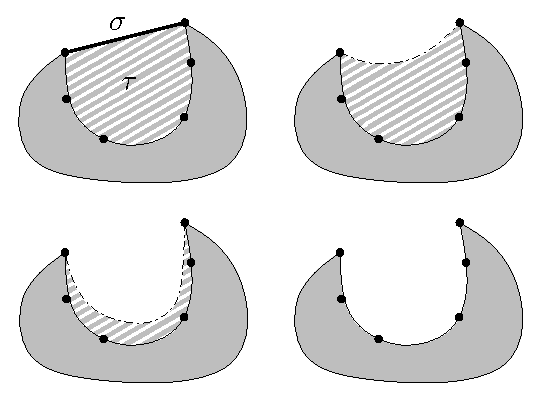
\includegraphics[width=80mm]{img/elementary-collapse.eps}
\caption{Elementarne zgniecenie.}\label{fig-elementary-collapse}
\end{figure}

Nietrudno spostrzec (zob.~rysunek \ref{fig-elementary-collapse}), że jeżeli $X\elcoll Y$, to $Y$~jest mocnym retraktem deformacyjnym $X$; co więcej, jeśli $\mP(Y)=\mP(X)\smallsetminus \{\sigma,\tau\}$, gdzie $\sigma$~jest właściwą ścianą $\tau$, to mocną retrakcję deformacyjną $r\colon X\to Y$ można wybrać w~ten sposób\label{mocna_retr_def_przy_el_zgnieceniu_ze_jest_fajna}, że \[r(\sigma\cup\tau)\subseteq \bigcup\{\rho\in \mP(Y):\rho \text{ jest ścianą } \tau \text{ w } X\}.\] 

Mówimy, że regularne CW kompleksy $X$, $Y$ mają ten sam \textit{prosty typ homotopijny}\index{typ homotopijny!prosty} (lub że są \textit{prosto homotopijnie równoważne}\index{homotopijna rozzzwnowazzzznoszzzczzz@homotopijna równoważność!prosta}), i~piszemy $X\simplehe Y$\nomenclature[7d]{$X\simplehe Y$}{regularne CW kompleksy $X$, $Y$ mają ten sam prosty typ homotopijny}, o~ile istnieje ciąg regularnych CW kompleksów $(X_i)_{i=0}^{n}$ taki, że $X_0=X$, $X_n=Y$ oraz dla każdego indeksu $i=0,\ldots,n-1$ zachodzi jeden z~warunków: $X_{i}\searrow X_{i+1}$ lub $X_{i+1}\searrow X_{i}$. Prosto homotopijnie równoważne CW kompleksy są, wobec obserwacji poczynionych w~poprzednim akapicie, homotopijnie równoważne.

Dobre wprowadzenie do interesującego fragmentu topologii algebraicznej, jaki stanowią zagadnienia związane z~prostym typem homotopijnym, stanowi książka Cohena \cite{Cohen73}.

Ponieważ każdy kompleks symplicjalny można utożsamiać z~pewnym regularnym CW kompleksem, możemy mówić o~prostym typie homotopijnym (oraz zgnieceniach itp.) kompleksów symplicjalnych.

Zdefiniujemy indukcyjnie związaną ze zgniatalnością kompleksów symplicjalnych własność, wywodzącą się z~teorii złożoności \cite{Kahn84}. Mówimy, że skończony kompleks symplicjalny $K$~jest \textit{non-evasive}\index{kompleks symplicjalny!non-evasive@\textit{non-evasive}}, jeśli $K$~składa się z~pojedynczego wierzchołka lub istnieje wierzchołek $v\in K$ taki, że kompleksy symplicjalne $\lk_K(v)$ oraz $K-v$ są \textit{non-evasive}. Jeżeli kompleks symplicjalny ma własność \mbox{\textit{non-evasiveness}}, to jest zgniatalny~\cite{Kahn84}.

\begin{tw}[{\cite[Theorem 2.10]{Welker99}}]\label{tw_welkera_o_zgniatalnosci_podzialu}
Jeśli skończony kompleks symplicjalny $K$~jest zgniatalny, to kompleks symplicjalny $\mK(\mP(K))$ ma własność \textit{non-evasiveness}.
\end{tw}


%====================================================================
%====================================================================
%====================================================================




\begin{comment}

\section{Geometria metryczna}\label{sec-geometria_metryczna}
Niech $(X,d)$ będzie przestrzenią metryczną. Określamy odległość punktu $x\in X$~od zbioru $A\subseteq X$ jako $d(x,A)=\inf\{a\in A:d(x,a)\}$.

\textit{Krzywą geodezyjną} (albo po prostu \textit{geodezyjną}) łączącą punkty $x,y\in X$ nazywamy odwzorowanie ciągłe $c\colon [0,l]\to X$ takie, że $c(0)=x, c(l)=y$ oraz $d(c(t),c(t'))=|t-t'|$ dla wszystkich $t,t'\in [0,l]$. W~szczególności mamy $l=d(x,y)$. \textit{Odcinkiem geodezyjnym} o~końcach $x,y$ nazywamy zbiór $c([0,l])\subseteq X$. Odcinek taki oznaczać będziemy czasem symbolem $[x,y]$. Istnieje wzajemnie jednoznaczna odpowiedniość pomiędzy geodezyjnymi w~$X$~a~parami $(x,\alpha)$, gdzie $\alpha$~jest odcinkiem geodezyjnym w~$X$~o~końcu $x$.

Mówimy, że przestrzeń $(X,d)$ jest \textit{geodezyjna}, jeśli dla każdej pary punktów $x,y\in X$ istnieje krzywa geodezyjna je łącząca. Dla $r>0$ przestrzeń $X$~nazywamy \textit{$r$-geodezyjną}, jeśli dla każdej pary punktów $x,y\in X$ takiej, że $d(x,y)<r$, istnieje geodezyjna je łącząca. 

Podzbiór $C$~geodezyjnej przestrzeni metrycznej $(X,d)$ nazywamy \textit{wypukłym}, jeśli każdą parę punktów $x,y\in C$ można połączyć geodezyjną w~$X$ oraz obraz każdej geodezyjnej łączącej te punkty zawiera się w~zbiorze $C$. \textit{Otoczką wypukłą} podzbioru geodezyjnej przestrzeni metrycznej nazywamy część wspólną wszystkich zbiorów wypukłych zawierających ten podzbiór.

Mówimy, że przestrzeń metryczna $(X,d)$ jest \textit{właściwa}, jeśli dla każdego $r\geq 0$ i~każdego $x\in X$ kula domknięta $D(x,r)=\{y\in X:d(x,y)\leq r\}$ jest zbiorem zwartym w~$X$. Przypomnijmy, że przestrzeń $(X,d)$ nazywamy \textit{zupełną}, gdy każdy ciąg Cauchy'ego w~$X$~jest zbieżny.

\textit{Średnicą} podzbioru $A\subseteq X$ przestrzeni metrycznej $(X,d)$ nazywamy liczbę $\operatorname{diam}(A)=\sup\{d(x,y):x,y\in A\}$.\nomenclature[ozn_srednica]{$\operatorname{diam}(A)$}{średnica zbioru $A$}

Dla $x,y\in\mR^n$ niech \[\langle x,y\rangle=\sum_{i=0}^{n-1}x_i y_i,\quad \langle\!\langle x,y\rangle\!\rangle=-x_{n-1}y_{n-1}+\sum_{i=0}^{n-2}x_i y_i\] oraz niech $\|x\|=\sqrt{\langle x, x\rangle}$

Zdefiniujemy dla $\kappa\in \mR$ oraz $n\in\mN$, $n\geq 1$ tzw.~\textit{przestrzenie modelowe} $M_\kappa^n$. Jeśli $\kappa>0$, to za $M_\kappa^n$ przyjmujemy sferę $\S^n$ z~metryką \[d(x,y)=\frac{1}{\sqrt{\kappa}} \operatorname{arccos}\left(\langle x,y\rangle\right)=\frac{2}{\sqrt{\kappa}} \operatorname{arcsin}\left(\frac{\|x-y\|}{2}\right).\]
Jeżeli $\kappa=0$, to $M^n_\kappa=\mathbb{R}^n$ z~metryką zadaną przez normę $\|\cdot\|$. Jeśli natomiast $\kappa<0$, to definiujemy $M^n_\kappa$ jako zbiór \[\mathbf{H}^n=\{x\in \mR^{n+1}:\langle\!\langle x,x\rangle\!\rangle=-1, x_{n}>0\}\] z~metryką zadaną dla $x,y\in \mathbf{H}^n$ wzorem \[d(x,y)=\frac{1}{\sqrt{-\kappa}}\operatorname{arccosh} (-\langle\!\langle x,y\rangle\!\rangle).\] 
\textit{Trójkątem geodezyjnym} $\Delta([x,y],[y,z],[z,x])$ w~przestrzeni metrycznej $(X,d)$ nazywamy układ trzech punktów $x,y,z\in X$ oraz łączących je odcinków geodezyjnych $[x,y], [y,z], [z,x]\subseteq X$. \textit{Trójkątem porównawczym} dla danego trójkąta geodezyjnego $\Delta([x,y],[y,z],[z,x])$ w~przestrzeni modelowej $M^2_\kappa$ nazywamy taki trójkąt geodezyjny $\Delta([\bar{x},\bar{y}],[\bar{y},\bar{z}],[\bar{z},\bar{x}])$ w~przestrzeni $M^2_\kappa$, że $d(x,y)=d(\bar{x},\bar{y})$, $d(y,z)=d(\bar{y},\bar{z})$, $d(z,x)=d(\bar{z},\bar{x})$. Trójkąt taki istnieje, o~ile zachodzi następująca nierówność dla długości obwodu tego trójkąta \[d(x,y)+d(y,z)+d(x,z)<2\operatorname{diam}(M^2_\kappa)=\begin{cases}\frac{2\pi}{\sqrt{\kappa}} & \text{dla } \kappa>0,\\\infty & \text{dla } \kappa\leq 0.\end{cases}\] Dla $p\in [x,y]$ \textit{punktem porównwawczym} w~trójkącie porównawczym $\Delta([\bar{x},\bar{y}],[\bar{y},\bar{z}],[\bar{z},\bar{x}])$ nazywamy taki element $\bar{p}\in [\bar{x},\bar{y}]$, że $d(x,p)=d(\bar{x},\bar{p})$; podobnie definiujemy punkty porównwacze dla elementów odcinków $[y,z],[z,x]$. Mówimy, że trójkąt geodezyjny $\Delta([x,y],[y,z],[z,x])$ spełnia \textit{nierówność $\CAT(\kappa)$}, jeśli długość obwodu tego trójkąta jest mniejsza niż $2\operatorname{diam}(M^2_\kappa)$ oraz dla wszystkich punktów $p,q\in [x,y]\cup [y,z]\cup [z,x]$ zachodzi nierówność $d(p,q)\leq d(\bar{p},\bar{q})$, gdzie $\bar{p},\bar{q}$ są punktami porównawczymi dla $p,q$ należącymi do trójkąta porównawczego dla trójkąta $\Delta([x,y],[y,z],[z,x])$ w~przestrzeni $M^2_\kappa$.

Jeśli $\kappa\leq 0$, to przestrzeń metryczną $X$~nazywamy \textit{przestrzenią $\CAT(\kappa)$}, jeżeli jest przestrzenią geodezyjną i~wszystkie trójkąty geodezyjne w~$X$~spełniają nierówność $\CAT(\kappa)$. Jeśli natomiast $\kappa>0$, to $X$~nazywamy \textit{przestrzenią $\CAT(\kappa)$}, gdy $X$~jest przestrzenią $\operatorname{diam}(M^2_\kappa)$-geodezyjną oraz wszystkie trójkąty geodezyjne w~$M^2_\kappa$ o~długości obwodu mniejszej niż $2\operatorname{diam}(M^2_\kappa)$ spełniają nierówność $\CAT(\kappa)$. Nazwa ,,$\CAT(\kappa)$'' została zaproponowana przez Gromova \cite{Gromov87} i~pochodzi od nazwisk E.~Cartana, A.D.~Aleksandrowa oraz V.A.~Toponogova. 

\begin{stw}[{\cite[Proposition II.1.4]{Bridson99}}]
Jeżeli $X$~jest przestrzenią $\CAT(\kappa)$, gdzie $\kappa\leq 0$ lub $\kappa>0$ oraz $\operatorname{diam}(X)<\frac{\pi}{\sqrt{\kappa}}$, to przestrzeń $X$~jest ściągalna.
\end{stw}

\begin{lem}[{\cite[Proposition II.2.4, Exercise II.2.6(1)] {Bridson99}}]\label{lemat-bridsona-o-jedynym-punkcie}
Niech $X$~będzie spójną przestrzenią $\CAT(\kappa)$, $x\in X$ jej elementem, zaś $C\subseteq X$ wypukłym, zupełnym podzbiorem. Jeżeli $\kappa\leq 0$ lub $\kappa\geq 0$ oraz $d(x,C)<\frac{\pi}{2\sqrt{\kappa}}$, to istnieje dokładnie jeden element $c\in C$ taki, że $d(x,c)=d(x,C)$.
\end{lem}

Niech $n\leq m$ będą dodatnimi liczbami naturalnymi oraz niech $\kappa\in\mathbb{R}$. \textit{Geodezyjnym $n$-wymiarowym sympleksem w~przestrzeni $M^m_\kappa$} nazywamy zbiór $S\subseteq M^m_\kappa$ będący otoczką wypukłą $n+1$ punktów $\{v_0,\ldots,v_n\}$ należących do $M^m_\kappa$ i~znajdujących się w~położeniu ogólnym, tzn.~nie zawierających się w~żadnej podprzestrzeni $M^m_\kappa$ izometrycznej z~$M^{n-1}_\kappa$, przy czym jeśli $\kappa>0$, to wymagamy dodatkowo, aby zbiór $\{v_0,\ldots,v_n\}$ zawierał się w~otwartej półsferze sfery $M^{m}_\kappa$. Elementy $v_0,\ldots,v_n\in M^m_\kappa$ nazywamy \textit{wierzchołkami} geodezyjnego sympleksu~$S$. Dla każdego punktu $s\in S$ określimy jego \textit{współrzędne barycentryczne} $b_0(s),\ldots,b_n(s)\in \I$. Jeżeli $\kappa=0$, to wierzchołki $v_0,\ldots,v_m$ są wektorami przestrzeni $M^m_\kappa=\mathbb{R}^{m}$. Współrzędne barycentryczne punktu $s$~określamy w~tym przypadku jako jedyne liczby z~odcinka jednostkowego $\I$ spełniające warunek \[x=b_0(s) v_0+\ldots+b_n(s) v_n.\] Jeśli $\kappa>0$, to $M^m_\kappa=\S^{m}\subseteq \mathbb{R}^{m+1}$. Otoczka wypukła wierzchołków $v_0,\ldots,v_n$ jest sympleksem $S'$ w~$\mathbb{R}^{m+1}$. Ponadto $0\not\in S'$, ponieważ wierzchołki te zawierają się w~otwartej półsferze sfery $\S^m$. Odwzorowanie $p\colon S\to S'$ zadane dla $x\in S'$ wzorem $p(x)=\frac{x}{\|x\|}$ jest bijekcją. Jako współrzędne barycentryczne punktu $s$~przyjmujemy współrzędne barycentryczne punktu $p^{-1}(s)$ w~sympleksie $S'$. Podobnie postępujemy dla $\kappa<0$. Współrzędne barycentryczne wyznaczają element $s\in S$ w~sposób jednoznaczny; możemy zatem $s$~utożsamiać z~funkcją $\tilde{s}\colon \{v_0,\ldots,v_n\}\to \I$ taką, że $\tilde{s}(v_i)=b_i(s)$.

Jeżeli $S, S'$ są $n$-wymiarowymi sympleksami geodezyjnymi odpowiednio w~$M^m_\kappa$ oraz $M^{m'}_{\kappa'}$, o~zbiorach wierzchołków $\{v_0,\ldots,v_n\}$ oraz $\{v_0',\ldots,v_{n}'\}$, to istnieje dokładnie jedno odwzorowanie $S\to S'$ zachowujące współrzędne barycentryczne i~przeprowadzające $v_i$ na $v_i'$ dla wszystkich $i=1,\ldots,n$. Podobnie, $\sigma\in K$ jest \mbox{$n$-wymiarowym} sympleksem kompleksu symplicjalnego $K$, $\sigma=\{v_0'',\ldots,v_n''\}$, to istnieje dokładnie jedno odwzorowanie $f\colon S\to |\sigma|$ z~sympleksu $S$~w~domknięty sympleks $|\sigma|\subseteq |K|$ takie, że $f(s)(v_i'')=\tilde{s}(v_i)$ dla $s\in S$ oraz wszystkich $i=1,\ldots,n$. Odwzorowania te, zwane \textit{afinicznymi}, są homeomorfizmami.

Kompleksem $M_\kappa$-symplicjalnym nazywamy trójkę \[\mathbb{K}=\left(K,\ \Shapes(\mathbb{K}),\ \{f_\sigma\colon S_\sigma\to |\sigma|\}_{\sigma\in K}\right),\] gdzie $K$~jest kompleksem symplicjalnym, $\Shapes(\mathbb{K})$ pewnym zbiorem geodezyjnych sympleksów w~przestrzeniach $M^{n}_\kappa$, $n\in\mN$, dla każdego sympleksu $\sigma$~istnieje geodezyjny, $\dim(\sigma)$-wymiarowy sympleks $S_\sigma\in \Shapes(\mathbb{K})$, a~$f_\sigma\colon S_\sigma\to |\sigma|$~jest afinicznym homeomorfizmem tego sympleksu na domknięty sympleks $|\sigma|\subseteq |K|$, przy czym jeżeli $\sigma,\tau\in K$ oraz $\sigma\subseteq \tau$, to odwzorowanie $f_\tau^{-1}\circ f_\sigma\colon S_\sigma \to S_\tau$ jest izometrią na obraz.

\textit{Nicią} w~kompleksie $M_\kappa$-symplicjalnym pomiędzy elementami $x,y\in |K|$ nazywamy ciąg $\Sigma=(x=x_0,x_1,\ldots,x_{n(\Sigma)}=y)$ elementów $K$~o~tej własności, że dla każdego $i=0,\ldots,n(\Sigma)-1$ istnieje sympleks $\sigma_i\in K$ taki, że $x_i,x_{i+1}\in |\sigma|$. \textit{Długością} nici $\Sigma$ nazywamy liczbę \[l(\Sigma)=\sum_{i=0}^{n(\Sigma)-1}d_{S_{\sigma_i}}\left(f_{\sigma_i}^{-1}(x_i),f_{\sigma_i}^{-1}(x_{i+1})\right),\]
gdzie $d_{S_{\sigma_i}}\colon S_{\sigma_i}\times S_{\sigma_i}\to \mathbb{R}$ jest funkcją odległości w~sympleksie $S_{\sigma_i}$. Jeśli kompleks symplicjalny $K$~jest spójny, określić można pewną funkcję $d_\mathbb{K}\colon |K|\times |K|\to \mathbb{R}$, dla $x,y\in |K|$ zadaną wzorem
\[d_\mathbb{K}(x,y)=\inf\{l(\Sigma): \Sigma\text{ jest nicią z } x \text{ do } y\}.\]
Na ogół tak zdefiniowana funkcja $d_\mathbb{K}$~nie jest metryką na $|K|$.

\begin{tw}[Bridsona, {\cite[Theorem I.7.19, Exercise I.7.62]{Bridson99}}]\label{tw-bridsona}
Jeżeli $\mathbb{K}=\left(K,\ \Shapes(\mathbb{K}),\ \{f_\sigma\}_{\sigma\in K}\right)$ jest kompleksem $M_\kappa$-symplicjalnym takim, że kompleks symplicjalny $K$~jest spójny oraz dla wszystkich $x\in |K|$ oraz $n\in \mN$ zbiór \[\bigl\{S_\sigma\in \Shapes(K):\sigma\in K,\ |\sigma|\subseteq \{y\in |K|: d_K(x,y)\leq n\}\bigr\}\] jest skończony, to  $(|K|,d_\mathbb{K})$ jest zupełną przestrzenią geodezyjną.
% oraz zbiór $\Shapes(K)$~jest skończony, to $(|K|,d_\mathbb{K})$ jest zupełną przestrzenią geodezyjną.

% Teza twierdzenia zachodzi również przy słabszym założeniu, że dla wszystkich $x\in |K|$ oraz $n\in \mN$ zbiór \[\bigl\{S_\sigma\in \Shapes(K):\sigma\in K,\ |\sigma|\subseteq \{y\in |K|: d_K(x,y)\leq n\}\bigr\}\] jest skończony.
\end{tw}

Kompleks $M_0$-symplicjalny $\mathbb{K}$~nazywamy \textit{regularnym}, o~ile długość wszystkich krawędzi każdego sympleksu $S\in\Shapes(\mathbb{K})$ wynosi $1$.

\end{comment}

%====================================================================
%====================================================================
%====================================================================





\section{Topologia w nieskończoności}\label{sec-top_w_nsk}
\textbf{Do końca podrozdziału \ref{sec-top_w_nsk} zakładamy, że $X$, $Y$~są przestrzeniami topologicznymi będącymi sumami rozłącznymi skończonej liczby uogólnionych continuów.} 

Podrozdział opiera się w~dużej mierze na książkach Bauesa i~Quintero~\cite{Baues01} oraz Hughesa i~Ranickiego \cite{Hughes96}.

\subsection{Właściwy typ homotopijny}
Jeżeli $f,g\colon X\to Y$ są właściwymi odwzorowaniami, to mówimy, że odwzorowania te są \textit{homotopijne w~sposób właściwy}, co oznaczamy przez $f\overset{p}{\simeq} g$\nomenclature[1m]{$f \overset{p}{\simeq} g$}{właściwe odwzorowania $f, g$ są homotopijne w~sposób właściwy}, jeżeli istnieje homotopia $H\colon X\times \I\to Y$ pomiędzy $f$ oraz~$g$ będąca właściwym odwzorowaniem (tzn.~\textit{właściwa homotopia}). Przestrzenie $X,Y$ nazywamy \textit{homotopijnie równoważnymi w~sposób właściwy}, jeżeli istnieje \textit{właściwa homotopijna równoważność}\index{homotopijna rozzzwnowazzzznoszzzczzz@homotopijna równoważność!wlzzzaszzzciwa@właściwa}\index{typ homotopijny!wlzzzaszzzciwy@właściwy} $X\to Y$, to znaczy takie właściwe odwzorowanie $f\colon X\to Y$, że dla pewnego właściwego odwzorowania $g\colon Y\to X$ istnieją właściwe homotopie $f\circ g\overset{p}{\simeq}\id_Y$ oraz~$g\circ f\overset{p}{\simeq}\id_X$.

Mówimy, że przestrzeń $X$~będąca ANR-em jest \textit{ściągalna w~sposób właściwy}\index{szzzciazzzgalnoszzzczzz w~sposozzzb wlzzzaszzzciwy@ściągalność w~sposób właściwy}\index{ANR!szzzciazzzgalny w~sposozzzb wlzzzaszzzciwy@ściągalny w~sposób właściwy}\index{przestrzenzzz topologiczna@przestrzeń topologiczna!szzzciazzzgalna w~sposozzzb wlzzzaszzzciwy@ściągalna w~sposób właściwy}, jeżeli przestrzeń $X$~jest homotopijnie równoważna w~sposób właściwy realizacji geometrycznej $1$-wymiarowego, lokalnie skończonego, spójnego i~acyklicznego kompleksu symplicjalnego (czyli drzewa).

\subsection{Zbiór końców}
Przez \textit{koniec}\index{koniec!przestrzeni topologicznej} przestrzeni $X$~rozumiemy odwzorowanie \[\varepsilon\colon \{K\subseteq X:K\text{ jest zwarty}\}\to 2^X\smallsetminus \{\emptyset\}\] takie, że dla wszystkich zbiorów zwartych $K,L\subseteq X$ spełnione są poniższe dwa warunki:
\begin{compactenum}
\item zbiór $\varepsilon(K)$ jest składową spójności przestrzeni $X\smallsetminus K$;
\item jeżeli $L\subseteq K$, to $\varepsilon(K)\subseteq \varepsilon(L)$.
\end{compactenum}
Symbolem $\E(X)$ oznaczamy zbiór wszystkich końców przestrzeni $X$\index{zbiozzzr@zbiór!konzzzcozzzw@końców!przestrzeni topologicznej}.
Podana definicja końca przestrzeni topologicznej pochodzi z~pracy Milnora \cite{Milnor68} i~dla uogólnionych continuów jest równoważna innym znanym definicjom końca (por.~\cite[Chapter~1]{Hughes96}).

\begin{ex}\noindent
\begin{compactenum}
\item Uogólnione continuum $X$~jest zwartą przestrzenią topologiczną wtedy i~tylko wtedy, gdy $\E(X)=\emptyset$.
\item Prosta rzeczywista $\mR$ ma dokładnie dwa końce, natomiast każda z przestrzeni $\mR^n$ dla $n\geq 2$ ma dokładnie jeden koniec.
\item Dla każdej liczby $n\in\mN$ przestrzeń \[X_n=\bigl( [0,\infty)\times \{0\} \bigr) \cup \bigl(\{0,\ldots,n-1\}\times [0,\infty)\bigr)\subseteq \mathbb{R}^2\] z~topologią indukowaną z~płaszczyzny $\mathbb{R}^2$ ma dokładnie $n+1$~końców. Ponadto zbiór końców przestrzeni $\bigcup_{n\in\mN} X_n$ jest przeliczalnie nieskończony.
\item Zbiór końców nakrycia uniwersalnego bukietu dwóch okręgów jest nieprzeliczalny.
\end{compactenum}
\end{ex}

Dla właściwego odwzorowania $f\colon X\to Y$ określimy indukowaną przez nie funkcję $\E(f)\colon \E(X)\to \E(Y)$. Jeżeli $\varepsilon\in \E(X)$ oraz $K\subseteq Y$ jest zbiorem zwartym, przyjmujemy za $\E(f)(\varepsilon)(K)$ tę spójną składową przestrzeni $Y\smallsetminus K$, dla której \[f\left(\varepsilon\left(f^{-1}(K)\right)\right)\subseteq \E(f)(\varepsilon)(K).\] Nietrudno zauważyć, że taka spójna składowa istnieje i~jest tylko jedna \cite[Proposition 1.22]{Hughes96}; ponadto $\E(f)(\varepsilon)\in \E(Y)$. Funkcja $\E(f)\colon \E(X)\to \E(Y)$ jest więc dobrze określona. Co więcej, łatwo sprawdza się, iż przyporządkowanie $\E$\nomenclature[6a]{$\E$}{funktor zbioru końców przestrzeni topologicznej (lub częściowego porządku)} jest funktorem z~kategorii przestrzeni topologicznych będących sumami rozłącznymi skończonej liczby uogólnionych continuów oraz ich właściwych odwzorowań w~kategorię zbiorów i~funkcji, oraz że jeśli właściwe odwzorowania $f,g\colon X\to Y$ są homotopijne w~sposób właściwy, to $\E(f)=\E(g)$ (zob.~\cite[Proposition 1.22]{Hughes96}).

Następujący lemat stanowi prosty wniosek z~lematu \ref{lem-sigma_zwarta_kazdy_zwarty_w_wyczerpujacym}.
\begin{lem}\label{lem-co_wyznacza_koniec_w_sigma_zwartej}
Załóżmy, że $(C_i)_{i\in\mN}$ jest ciągiem wyczerpującym przestrzeń $X$. Niech $Z$~oznacza zbiór funkcji $\delta\colon \{C_i\}_{i\in\mN}\to 2^X\smallsetminus \{\emptyset\}$ takich, że dla każdego $i\in\mN$ zbiór $\delta(C_i)$~jest nieograniczoną składową spójności przestrzeni $X\smallsetminus C_i$ oraz $\delta(C_j)\subseteq \delta(C_i)$ dla $j\geq i$. Funkcja $\E(X)\to Z$ przyporządkowująca końcowi $\varepsilon\in \E(X)$ jego ograniczenie $\varepsilon\big |_{\{C_i\}_{i\in\mN}}$ jest bijekcją.
\end{lem}

\begin{lem}\label{lem-istnieje_koniec_w_strone_danej_skladowej}
Niech $K$~będzie zwartym podzbiorem $X$, zaś~$S$ nieograniczoną w~$X$~składową spójności zbioru $X\smallsetminus K$. Istnieje wówczas koniec $\varepsilon\in\E(X)$ taki, że $\varepsilon(K)=S$.
\end{lem}
\begin{proof}
Na podstawie lematu \ref{lem-istnieje_ciag_wyczerpujacy} istnieje wyczerpujący przestrzeń $X$~ciąg $(C_i)_{i\in\mN}$ taki, że $C_0=K$. Określimy pewną funkcję $\delta\colon \{C_i\}_{i\in \mN}\to 2^X\smallsetminus\{\emptyset\}$. Niech $\delta(C_0)=S$. Ustalmy $n>0$ i~załóżmy, że dla wszystkich liczb naturalnych $i<n$ określone są zbiory $\delta(C_i)\in 2^X\smallsetminus\{\emptyset\}$, przy czym $\delta(C_i)$ jest nieograniczoną składową spójności $X\smallsetminus C_i$ oraz $\delta(C_j)\subseteq \delta(C_i)$ dla wszystkich $i\leq j<n$. Za $\delta(C_{n})$ przyjmujemy dowolną nieograniczoną składową spójności zbioru $X\smallsetminus C_{n}$ zawartą w~$\delta(C_{n-1})$.

Wobec lematu \ref{lem-co_wyznacza_koniec_w_sigma_zwartej} istnieje koniec $\varepsilon\in \E(X)$ taki, że $\varepsilon\big|_{\{C_i\}_{i\in\mN}}=\delta$. W~szczególności $\varepsilon(K)=\delta(K)=S$.
\end{proof}



%--------------------------------------------------------------------
%-------------------------------------------------------------------
%-------------------------------------------------------------------


\subsection{Uzwarcenie Freudenthala}
Dla końca $\varepsilon\in \E(X)$ oraz zwartego zbioru $K\subseteq X$ przyjmijmy oznaczenia \begin{align*}B(\varepsilon,K)&=\{\varepsilon'\in \E(X): \varepsilon(K)=\varepsilon'(K)\},\\N(\varepsilon,K)&=\varepsilon(K)\cup B(\varepsilon,K).\end{align*} 

\textit{Uzwarceniem Freudenthala}\index{uzwarcenie!Freudenthala} \cite{Freudenthal31, Raymond60} przestrzeni $X$~nazywamy przestrzeń $\F X=X\cup \E(X)$ z~topologią zadaną przez następujące bazy otoczeń otwartych: dla $x\in X$ jako bazę otoczeń otwartych przyjmujemy dowolną bazę otoczeń otwartych tego punktu w~przestrzeni $X$, natomiast dla końca $\varepsilon\in\E(X)$ bazą otoczeń otwartych jest rodzina $\{N(\varepsilon,K): K\subseteq X\text{ jest zbiorem zwartym}\}$.

Niech $f\colon X\to Y$ będzie właściwym odwzorowaniem. Określmy funkcję $\F f\colon \F X\to \F Y$ dla elementu $a\in \F X$ przyjmując \[\F f(a)=\begin{cases}f(a), &\text{jeżeli } a\in X,\\ \E(f)(a), & \text{jeżeli } a\in\E(X).\end{cases}\]

\begin{stw}[{\cite[Proposition I.9.11]{Baues01}}]\label{stw-funkcja_freudenthala_ciagla}
Jeśli $f\colon X\to Y$ jest właściwym odwzorowaniem, to funkcja $\F f\colon \F X\to \F Y$ jest ciągła.
\end{stw}

Wobec stwierdzenia \ref{stw-funkcja_freudenthala_ciagla} przyporządkowanie $\F$ jest  funktorem\nomenclature[6b]{$\F$}{funktor uzwarcenia Freudenthala} z~kategorii przestrzeni topologicznych będących sumami rozłącznymi skończonej liczby uogólnionych continuuów i~ich właściwych odwzorowań w~kategorię przestrzeni topologicznych i~funkcji ciągłych.

\begin{comment}
Uzwarcenie Freudenthala można scharakteryzować w~następujący sposób.

\begin{tw}[\cite{Raymond60}]\label{tw-raymonda}
Niech $X^*$ będzie uzwarceniem przestrzeni $X$ o~następujących własnościach:
\begin{compactenum}
\item przestrzeń $X^*$ jest spójna;
\item $X$ jest otwartym podzbiorem $X^*$;
\item przestrzeń $X^*\smallsetminus X$ jest całkowicie niespójna;
\item jeśli $p\in X^*\smallsetminus X$ oraz $U$~jest spójnym otoczeniem otwartym punktu $p$, to zbiór $U\smallsetminus (X^*\smallsetminus X)$ jest spójny.
\end{compactenum}
Wówczas uzwarcenie $X^*$ jest izomorficzne z~uzwarceniem Freudenthala $\F X$.
\end{tw}
\end{comment}

\begin{lem}[{\cite[Addendum I.9.9]{Baues01}}]\label{lem-uzwarcenie_jest_metryczne}
Jeżeli $X$~jest uogólnionym continuum, to $\F X$~jest continuum. Jeśli $X$~jest uogólnionym continuum Peano, to $\F X$~jest continuum Peano.
\end{lem}

\begin{comment}
\begin{lem}\label{lem-iloraz_homeomorficzny_jednopunktowemu}
Jeśli przestrzeń $X$~jest niezwarta, to przestrzeń ilorazowa $\F X\big/\E(X)$ jest homeomorficzna $X^\infty$.
\end{lem}
\begin{proof}
Ustalmy niezwartą przestrzeń $X$~będącą sumą rozłączną skończonej liczby uogólnionych continuów. Rozważmy funkcję $f\colon \F X\to X^\infty$ zadaną dla $a\in \F X$ wzorem \[f(a)=\begin{cases} a, & \text{jeżeli } a\in X,\\ \infty^X, &\text{jeżeli } a\in \E(X).\end{cases}\]

Oczywiście $\E(X)\not=\emptyset$, więc $f$~jest surjekcją. Jeżeli $U=\bigl\{\infty^X\bigr\}\cup (X\smallsetminus K)$ dla pewnego zbioru zwartego $K\subseteq X$, to \[f^{-1}(U)=(X\smallsetminus K)\cup \E(X)=(X\smallsetminus K)\cup \bigcup_{\varepsilon\in \E(X)}N(\varepsilon,K)\] jest zbiorem otwartym w~$\F X$. Wobec przyjętej definicji topologii na przestrzeni $X^\infty$ przekształcenie $f$~jest więc ciągłe. Wykażemy, że $f$~jest odwzorowaniem ilorazowym, tzn.~że topologia na $X^\infty$ jest najbogatszą spośród topologii na tym zbiorze, przy których funkcja $f$~jest ciągła, co będzie oznaczało, że $X^\infty\approx \F X\big/\E(X)$.

Rozważmy w~tym celu taki podzbiór $U\subseteq X^\infty$, że zbiór $f^{-1}(U)\subseteq \F X$ jest otwarty. Jeżeli $\infty^X\not\in U$, to $f^{-1}(U)=U\subseteq X$ jest zbiorem otwartym w~$X$, a~zatem również w~$X^\infty$. Jeśli natomiast $\infty^X\in U$, to $\E(X)\subseteq f^{-1}(U)$. Możemy więc przedstawić zbiór $f^{-1}(U)$ jako sumę \[f^{-1}(U)=V\cup \bigcup_{\varepsilon\in \E(X)}\bigcup_{K\in \mathfrak{K}(\varepsilon)} N(\varepsilon, K),\] gdzie $V$~jest otwartym podzbiorem $X$, zaś $\mathfrak{K}(\varepsilon)\subseteq 2^{X}$ jest, dla każdego końca $\varepsilon\in\E(X)$, pewną rodziną zwartych podzbiorów przestrzeni $X$. Ponieważ $X$~jest otwartym podzbiorem zwartej przestrzeni $\F X $, zbiór $\E(X)=\F X\smallsetminus X$ jest zwarty. Rodzina \[\left\{N(\varepsilon,K):\varepsilon\in\E(X), K\in\mathfrak{K}(\varepsilon)\right\}\] jest otwartym pokryciem $\E(X)$. Można zatem wybrać końce $\varepsilon_1,\ldots, \varepsilon_n\in \E(X)$ oraz zbiory zwarte $K_i\in\mathfrak{K}(\varepsilon_i)$, $i=1,\ldots, n$, o~tej własności, że skończona rodzina $\{N(\varepsilon_i,K_{i})\}_{i=1}^{n}$ jest otwartym pokryciem zbioru $\E(X)$. W~szczególności, dla każdego końca $\delta\in \E(X)$ istnieje indeks $i_\delta\in \{1,\ldots, n\}$ taki, że $\delta\in N\left(\varepsilon_{i_\delta},K_{i_\delta}\right)$, to znaczy $\delta\left(K_{i_\delta}\right)=\varepsilon_{i_\delta}\left(K_{i_\delta}\right)$. Zbiór $\bigcup_{i=1}^{n}K_i\subseteq X$ jest zwarty jako skończona suma zbiorów zwartych. Na podstawie lematu \ref{lem-dorzucanie_skladowych_a_zwartosc} istnieje zwarty podzbiór $\hat{K}\subseteq X$ zawierający $\bigcup_{i=1}^{n}K_i$ oraz~taki, że każda składowa spójności zbioru $X\smallsetminus \hat{K}$ jest nieograniczona w~$X$. Dla dowolnego końca $\delta\in \E(X)$ mamy \[\delta\left(\hat{K}\right)\subseteq \delta\left(K_{i_\delta}\right)=\varepsilon_{i_\delta}\left(K_{i_\delta}\right)\subseteq B\left(\varepsilon_{i_\delta},K_{i_\delta}\right)\subseteq U.\] Ponadto, na podstawie lematu \ref{lem-istnieje_koniec_w_strone_danej_skladowej} każda składowa spójności zbioru $X\smallsetminus \hat{K}$ jest postaci $\delta\left(\hat{K}\right)$ dla pewnego końca $\delta\in \E(X)$. Wobec tego $X\smallsetminus \hat{K}\subseteq U$. Zbiór $f^{-1}(U)$ możemy  przedstawić jako poniższą sumę:
\[f^{-1}(U)=V\cup \left(\left(X\smallsetminus \hat{K}\right)\cup \E(X)\right)\cup \bigcup_{\varepsilon\in \E(X)}\bigcup_{K\in \mathfrak{K}(\varepsilon)} \varepsilon(K).\]
Ale zbiór \[V\cup \bigcup_{\varepsilon\in \E(X)}\bigcup_{K\in \mathfrak{K}(\varepsilon)} \varepsilon(K)\] jest otwarty w~$X$. Wobec tego \[U=\left(V\cup \bigcup_{\varepsilon\in \E(X)}\bigcup_{K\in \mathfrak{K}(\varepsilon)} \varepsilon(K)\right)\cup \left(\left(X\smallsetminus \hat{K}\right)\cup \left\{\infty^X\right\}\right)\] jest otwartym podzbiorem $X^\infty$, co kończy dowód lematu.
\end{proof}
\end{comment}




%--------------------------------------------------------------------
%-------------------------------------------------------------------
%-------------------------------------------------------------------



\subsection{Oswojoność}
Przestrzeń $X$ nazywamy \textit{oswojoną na zewnątrz}\footnote{ang. \textit{outward tame}}\index{przestrzenzzz topologiczna@przestrzeń topologiczna!oswojona na zewnazzztrz@oswojona na zewnątrz} \cite{Quinn88,Hughes96}, jeżeli istnieje domknięty, koograniczony podzbiór $V\subseteq X$ taki, że włożenie $V\times \{0\}\hookrightarrow X$ (dla $v\in V$ zadane wzorem $(v,0)\mapsto v$) rozszerza się do właściwego odwzorowania $V\times [0,\infty)\to X$.

Mówimy, że przestrzeń $X$~\textit{ma kołnierzyk na zewnątrz}\footnote{ang. \textit{is outward collared}} \cite{Hughes96}\index{przestrzenzzz topologiczna@przestrzeń topologiczna!ma kolzzznierzyk na zewnazzztrz@ma kołnierzyk na zewnątrz}, jeżeli istnieje domknięty, koograniczony podzbiór $V\subseteq X$ będący ANR-em i~taki, że włożenie $V\times\{0\}\hookrightarrow V$ rozszerza się do właściwego odwzorowania $V\times [0,\infty)\to V$. (Oczywiście każda przestrzeń z~kołnierzykiem na zewnątrz jest oswojona na zewnątrz.)

\begin{comment}
\begin{tw}[{\cite[Proposition 7.2]{Hughes96}}]\label{tw-kolnierzyk_na_zewnatrz_a_brzeg_waldhausena}
Niech $X$~będzie przestrzenią z~kołnierzykiem na zewnątrz oraz niech podzbiór $V\subseteq X$ ma własności jak w~powyższej definicji. Istnieją wówczas homotopijne równoważności $e(X)\simeq e(V)\simeq V$.
\end{tw}
\end{comment}


\begin{ex}[{\cite[Example 7.3]{Hughes96}}]\noindent
\begin{compactenum}
\item Niech $M$~będzie zwartą rozmaitością z~brzegiem $\partial M$. Wówczas przestrzeń $X=M\smallsetminus \partial M$ ma kołnierzyk na zewnątrz. % oraz $e(X)\simeq \partial M$.
\item Niech $\left(f_j\colon X_j\to X_{j+1}\right)_{j\in\mN}$ będzie systemem prostym przekształceń pomiędzy zwartymi ANR-ami. \textit{Teleskopem} tego systemu nazywamy przestrzeń \[\operatorname{Tel}\left(f_j\right)_{j\in\mN}=\left(\coprod_{j=0}^{\infty} (X_j\times \I)\right)\big/\sim\ ,\] gdzie $\sim$~jest najmniejszą relacją równoważności na zbiorze $\coprod_{j=0}^\infty (X_j\times \I)$ taką, że $(x_j,1)\sim (f_j(x_j),0)$ dla wszystkich $x_j\in X_j$, $j\in\mN$. Teleskop $\operatorname{Tel}\left(f_j\right)_{j\in\mN}$ ma kołnierzyk na zewnątrz.
\item Niech $X$~będzie przestrzenią topologiczną, $A\subseteq X$ jej podzbiorem, $U\subseteq X$ otoczeniem $A$ oraz niech $V\subseteq U$. Mówimy, że zbiór~$V$~jest \textit{I-kompresowalny} w~$U$ w~kierunku $A$, jeżeli dla każdego otoczenia $W\subseteq X$ zbioru $A$~istnieje izotopia $(h_t)_{t\in \I}$ taka, że \[h_0=\id_X,\quad h_1(V)\subseteq W, \quad h_t\big|_{Z\cup X\smallsetminus U}=\id_{Z\cup X\smallsetminus U}\] dla pewnego otoczenia $Z$~zbioru $A$~oraz wszystkich $t\in \I$. Jeśli dla każdego otoczenia $U$~zbioru $A\subseteq X$ istnieje otoczenie $V\subseteq U$~tego zbioru o~tej własności, że $V$~jest I-kompresowalne w~$U$~w~kierunku $A$, to mówimy, że $A$~ma \textit{otoczenie I-regularne} w~$X$ (zob. \cite{Siebenmann73}).

Niech $A$~będzie zwartym podzbiorem wnętrza zwartej rozmaitości $M$. Jeśli $A$~ma I-regularne otoczenie w~$M$, to przestrzeń $M\smallsetminus A$ jest oswojona na zewnątrz. Jest tak w~szczególności, gdy przestrzeń $A$~ma typ homotopijny (czy ogólniej kształt) CW kompleksu i~jest 1-LCC zanurzona w~$M$ (tzn.~dla każdego $a\in A$ i~otwartego otoczenia $U$~tego punktu w~$M$ istnieje otoczenie otwarte $a\in V\subseteq U$ takie, że każde ciągłe przekształcenie $\S^1\to V\smallsetminus A$ rozszerza się do ciągłego odwzorowania $\D^2\to U\smallsetminus A$).
\item Więcej przykładów przestrzeni oswojonych na zewnątrz odnaleźć można w~książce Hughesa i~Ranickiego \cite{Hughes96}.
\end{compactenum}
\end{ex}

Przestrzeń $X$~nazywamy \textit{oswojoną do wewnątrz}\index{przestrzenzzz topologiczna@przestrzeń topologiczna!oswojona do wewnazzztrz@oswojona do wewnątrz}\footnote{ang. \textit{inward tame}}\label{def-osw_do_wew} \cite{Chapman76,Hughes96}, o~ile dla każdego koograniczonego podzbioru $U\subseteq X$ istnieją koograniczony w~$X$~podzbiór $V\subseteq U$ oraz homotopia $h\colon X\times \I\to X$ o~następujących własnościach:
\begin{compactitem}
\item[---] $h_0=\id_X$;
\item[---] $h(x,t)=x$ dla wszystkich $x\in X\smallsetminus U$, $t\in \I$;
\item[---] $h(U\times \I)\subseteq U$;
\item[---] $h_1(X)\subseteq X\smallsetminus V$. 
\end{compactitem}

Mówimy, że przestrzeń $X$~\textit{ma kołnierzyk do wewnątrz}\footnote{ang. \textit{is inward collared}}\index{przestrzenzzz topologiczna@przestrzeń topologiczna!ma kolzzznierzyk do wewnazzztrz@ma kołnierzyk do wewnątrz} \cite{Hughes96}, jeśli dla każdego koograniczonegu podzbioru $U\subseteq X$ istnieje koograniczony w~$X$~podzbiór $V\subseteq U$ o~tej własności, że $U\smallsetminus V$ jest mocnym retraktem deformacyjnym $U$. Przestrzeń mająca kołnierzyk do wewnątrz jest oswojona do wewnątrz.

\begin{tw}[{\cite[Proposition 8.5]{Hughes96}}]\label{tw-charakteryzacja_kolnierzyka_do_wewnatrz}
Przestrzeń $X$~będąca ANR-em ma kołnierzyk do wewnątrz wtedy i~tylko wtedy, gdy istnieje wstępujący ciąg $(K_i)_{i=0}^{\infty}$ zwartych ANR-ów taki, że $X=\bigcup_{n\in\mN} K_n$ oraz każde z~włożeń $K_n\hookrightarrow X$, $n\in\mN$, jest homotopijną równoważnością.
\end{tw}

\begin{ex}[\cite{Guilbault13,Hughes96}]\label{przyklady-oswojonych-do-wewnatrz}\noindent
\begin{compactenum}
\item Niech $X$~będzie ANR-em. Domknięty podzbiór $A\subseteq X$~ nazywamy \mbox{\textit{$\mathcal{Z}$-zbiorem}} w~$X$, jeżeli dla każdego otwartego zbioru $U\subseteq X$ włożenie $U\smallsetminus A\hookrightarrow U$ jest homotopijną równoważnością. Przykładowo, każdy domknięty podzbiór brzegu rozmaitości $M$~jest $\mathcal{Z}$-zbiorem w~$M$. Uzwarcenie $X^*$~przestrzeni $X$~takie, że $X^*\smallsetminus X$ jest $\mathcal{Z}$-zbiorem w~$X^*$, nazywamy \textit{\mbox{$\mathcal{Z}$-uzwarceniem}}\index{uzwarcenie!zuzwarcenie@$\mathcal{Z}$-uzwarcenie}\index{zuzwarcenie@$\mathcal{Z}$-uzwarcenie}. Każdy ANR mający $\mathcal{Z}$-uzwarcenie jest przestrzenią oswojoną do wewnątrz.
\item W~szczególności, przestrzenie postaci $M\smallsetminus \partial M$, gdzie $M$~jest zwartą rozmaitością z~brzegiem, są oswojone do wewnątrz. Co więcej, przestrzenie tego typu mają kołnierzyk do wewnątrz \cite[Example 8.3]{Hughes96}.
\item Dla $n\geq 4$ istnieją zwarte, asferyczne, $n$-wymiarowe rozmaitości bez brzegu, których nakrycia uniwersalne nie są homeomorficzne z~$\mR^n$. Sztandarowym przykładem są tzw.~rozmaitości Davisa \cite{Guilbault13}. Rozmaitości Davisa nie są postaci $M\smallsetminus \partial M$ dla żadnej zwartej rozmaitości $M$. Istnieją jednak ich \mbox{$\mathcal{Z}$-uzwarcenia}, przy czym narosty tych uzwarceń nie są ANR-ami. Rozmaitości Davisa są oswojone do wewnątrz.
\item Rozważmy system odwrotny $\left(f_j\colon X_{j+1}\to X_j\right)_{j\in\mN}$ ciągłych odwzorowań pomiędzy zwartymi ANR-ami. \textit{Odwrotnym teleskopem} tego systemu nazywamy przestrzeń \[\operatorname{InvTel}\left(f_j\right)_{j\in\mN}=\left(\coprod_{j=0}^{\infty}(X_j\times \I)\right)\big/\sim\ ,\]
gdzie $\sim$~jest najmniejszą relacją równoważności na sumie rozłącznej $\coprod_{j=0}^{\infty}(X_j\times \I)$ taką, że $(x_j,0)\sim (f_j(x_j),1)$ dla wszystkich $x_j\in X_j$, $j\in\mN$. Przestrzeń $\operatorname{InvTel}\left(f_j\right)_{j\in\mN}$ ma kołnierzyk do wewnątrz. (Ma ona również \mbox{$\mathcal{Z}$-uzwarcenie}.)
\item Każda przestrzeń metryczna $X$, której metryka jest właściwa (tzn.~domknięte, ograniczone względem tej metryki podzbiory przestrzeni $X$~są zwarte) i~ma tzw.~własność $\CAT(0)$ \cite{Bridson99}, jest oswojona do wewnątrz. (Co więcej, przestrzenie takie mają \mbox{$\mathcal{Z}$-uzwarcenia} \cite[Example 17.5.5]{Geoghegan08}.)
\item Inne przykłady przestrzeni oswojonych do wewnątrz odnaleźć można w~książce Hughesa i~Ranickiego \cite{Hughes96}.
\end{compactenum}
\end{ex}


%--------------------------------------------------------------------
%--------------------------------------------------------------------
%--------------------------------------------------------------------




\subsection{Homologie lokalnie skończone i~homologie w~nieskończoności}
Ustalmy $n\in \mN$. Przypomnijmy, że \mbox{$n$-wymiarowym} \textit{sympleksem singularnym}\index{sympleks!singularny} w~przestrzeni topologicznej $X$~nazywamy ciągłe przekształcenie $\sigma\colon \Delta^n\to X$ standardowego, $n$-wymiarowego sympleksu domkniętego w~tę przestrzeń. Wszystkie $n$-wymiarowe sympleksy singularne w~przestrzeni $X$~tworzą zatem zbiór elementów przestrzeni $\Cont(\Delta^n,X)$.

Dla każdej liczby $n\in\mN$~na zbiorze wszystkich funkcji $\Cont(\Delta^n,X)\to \mathbb{Q}$ istnieje naturalna struktura przestrzeni liniowej nad ciałem liczb wymiernych (z~działaniami ,,po współrzędnych''). Rozważmy jej podprzestrzeń liniową $S^{\lf}_n(X)$, której elementami są funkcje $z\colon \Cont(\Delta^n,X)\to \mathbb{Q}$ mające tę własność, że dla każdego elementu $x\in X$ istnieje jego otwarte otoczenie $U\subseteq X$ takie, że zbiór \[\left\{\sigma\in \Cont(\Delta^n,X): \sigma(\Delta^n)\cap U\not=\emptyset,\ z(\sigma)\not=0\right\}\] jest skończony. Przestrzeń liniową $S^\lf_n(X)$ nazywamy przestrzenią \textit{\mbox{$n$-wymiarowych}, lokalnie skończonych łańcuchów singularnych}~$X$~(o~współczynnikach wymiernych).

Dla $n\in \mN$ oraz $0\leq i\leq n+1$ przez $e^i_{n+1}\colon \Delta^n\to \Delta^{n+1}$ oznaczamy ciągłe odwzorowanie zadane dla $(x_0,\ldots,x_n)\in \Delta^n$ wzorem \[e^i_{n+1}(x_0,\ldots,x_n)=(x_0,\ldots,x_{i-1},0,x_{i},\ldots,x_{n}).\] Istnieje homomorfizm liniowy $d_{n+1}^\lf\colon S^\lf_{n+1}(X)\to S^\lf_n(X)$ zadany dla $z\in S^\lf_{n+1}(X)$ oraz $\tau\in \Cont(\Delta^n,X)$ wzorem 
\[d_{n+1}^\lf(z)(\tau)=\sum_{i=0}^{n+1}\ \sum_{\substack{\sigma\in \Cont(\Delta^{n+1},X),\\ \sigma \circ e^i_{n+1}=\tau}} (-1)^i z(\sigma).\] Nietrudno sprawdzić, że homomorfizm ten jest dobrze określony, a~ponadto dla każdego $n\geq 1$ zachodzi równość $d^\lf_n\circ d^\lf_{n+1}=0$. 

\index{kompleks!lokalnie skonzzzczonych lzzzannncuchozzzw@lokalnie skończonych łańcuchów}\textit{Kompleksem lokalnie skończonych łańcuchów singularnych przestrzeni topologicznej $X$}~nazywamy kompleks łańcuchowy $S^{\lf}_*(X)=\left(S^{\lf}_n(X),d^\lf_n\right)_{n\in\mN}$. \textit{Lokalnie skończonymi homologiami singularnymi przestrzeni $X$}\index{homologie!lokalnie skonzzzczone@lokalnie skończone}~\cite[Definition 3.1]{Hughes96}~nazywamy przestrzeń wektorową z~gradacją $H_*^{\lf}(X)$ (nad ciałem liczb wymiernych) uzyskaną przez zadziałanie na kompleksie łańcuchowym $S_*^{\lf}(X)$ funktorem homologii: \[H_*^{\lf}(X)=H_*\left(S_*^{\lf}(X)\right).\]

Właściwe odwzorowanie $X\to Y$ indukuje homomorfizm grup homologii lokalnie skończonych \cite[Proposition 3.2]{Hughes96}; fakt ten podano w~książce Hughesa i~Ranickiego bez dowodu. Dla wygody Czytelnika przedstawiamy go poniżej.

Następujący lemat jest prostą konsekwencją definicji zbioru zwartego.
\begin{lem}\label{lem-lok_sk_lancuch_ze_zb_zwartym_sie_tnie}
Jeżeli $z\in S^{\lf}_n(X)$ dla pewnego $n\in\mN$ oraz zbiór $K\subseteq X$ jest zwarty, to istnieje otwarty podzbiór $U\subseteq X$ taki, że $K\subseteq U$ oraz zbiór \[\{\sigma\in \Cont(\Delta^n,X):\sigma(\Delta^n)\cap U\not=\emptyset,\ z(\sigma)\not=0\}\] jest skończony.
\end{lem}

Jeżeli $f\colon X\to Y$ jest właściwym odwzorowaniem, to dla każdego $n\in\mN$ istnieje homomorfizm liniowy $S_n^{\lf}(f)\colon S_n^{\lf}(X)\to S_n^{\lf}(Y)$, zadany dla $z\in S^{\lf}_n(X)$ oraz $\tau\in \Cont(\Delta^n,Y)$ wzorem \begin{equation}S_n^{\lf}(f)(z)(\tau)=\sum_{\substack{\sigma\in \Cont(\Delta^n,X),\\f\circ\sigma=\tau}} z(\sigma).\label{eq-homomorfizm_indukowany_na_h_lf}\end{equation}
Należy wykazać, że homomorfizm ten jest dobrze określony, tzn.~suma w~powyższym wzorze jest skończona dla wszystkich $z\in S^{\lf}_n(X)$, $\tau\in\Cont(\Delta^n,X)$ oraz dla każdego punktu $y\in Y$~istnieje jego otwarte otoczenie $U\subseteq Y$ takie, że zbiór \[\left\{\tau\in \Cont(\Delta^n,Y):\tau(\Delta^n)\cap U\not=\emptyset,\ S^\lf_n(f)(z)(\tau)\not=0\right\}\] jest skończony.

Ustalmy w~tym celu $z\in S^\lf_n(X)$ oraz $\tau\in \Cont(\Delta^n,Y)$. Odwzorowanie $f$~jest właściwe, więc zbiór $f^{-1}(\tau(\Delta^n))\subseteq X$ jest zwarty. Na podstawie lematu \ref{lem-lok_sk_lancuch_ze_zb_zwartym_sie_tnie} zbiór \[\left\{\sigma\in\Cont(\Delta^n,X):\sigma(\Delta^n)\cap f^{-1}(\tau(\Delta^n))\not=\emptyset,\ z(\sigma)\not=0\right\}\] jest skończony. Ze skończoności tego zbioru oraz zawierania \[\left\{\sigma\in\Cont(\Delta^n,X):f\circ\sigma=\tau\right\}\subseteq \left\{\sigma\in\Cont(\Delta^n,X):\sigma(\Delta^n)\subseteq f^{-1}(\tau(\Delta^n))\right\}\] wynika, że suma we wzorze (\ref{eq-homomorfizm_indukowany_na_h_lf}) jest skończona. Przestrzeń $Y$~jest lokalnie zwarta, więc dla każdego elementu $y\in Y$ istnieje jego otwarte otoczenie $U\subseteq Y$ o~zwartym domknięciu. Zbiór $f^{-1}\left(\overline{U}\right)\subseteq X$ jest zwarty, gdyż funkcja $f$~jest właściwa; wobec lematu \ref{lem-lok_sk_lancuch_ze_zb_zwartym_sie_tnie} zbiór \[A=\left\{\sigma\in\Cont(\Delta^n,X):\sigma(\Delta^n)\cap f^{-1}\left(\overline{U}\right)\not=\emptyset,\ z(\sigma)\not=0\right\}\] jest skończony, a~zatem skończony jest też zbiór \[\left\{\tau\in\Cont(\Delta^n,Y):\tau(\Delta^n)\cap U\not=\emptyset,\ S^\lf_n(f)(z)(\tau)\not=0\right\}\subseteq \left\{(f\circ \sigma)
:\sigma\in A\right\}.\]

Jak nietrudno sprawdzić, ciąg $\left(S^{\lf}_n(f)\right)_{n\in\mN}$ jest homomorfizmem kompleksów łańcuchowych $S_*^\lf(f)\colon S_*^\lf(X)\to S_*^\lf(Y)$, a~zatem indukuje homomorfizm $H^\lf_*(f)\colon H_*^{\lf}(X)\to H_*^\lf(Y)$. Przyporządkowanie $H_*^{\lf}~$\nomenclature[1yb]{$H_*^{\lf}$}{funktor lokalnie skończonych homologii} jest funktorem z~kategorii przestrzeni lokalnie zwartych i~ich właściwych odwzorowań w~kategorię przestrzeni wektorowych~z~gradacją (nad ciałem liczb wymiernych) i~homomorfizmów liniowych zachowujących gradację. Ponieważ nie będziemy rozważać innych niż singularne homologii lokalnie skończonych, funktor lokalnie skończonych homologii singularnych nazywać będziemy krótko funktorem \textit{lokalnie skończonych homologii}.

Część autorów stosuje odmienną terminologię, funktor $H_*^{\lf}$~nazywając funktorem homologii Borela-Moore'a.\index{homologie!Borela-Moore'a} Zdarza się, że nazwa ta jest rezerwowana dla funktorów zdefiniowanych w~inny sposób; możliwości jest kilka (przykładowo, definicja pochodząca z~pracy Borela i~Moore'a \cite{Borel60} korzysta z~teorii snopów). Dla ,,dostatecznie dobrych'' przestrzeni wszystkie te funktory są równoważne \cite[Section 2.6]{Chriss10}. Autor sądzi, że nazwa ,,homologie lokalnie skończone'' dobrze wyraża, jaki funktor mamy na myśli, i~pozwala uniknąć zamieszania wynikającego z~niejednoznaczności terminologii związanej z~homologiami Borela-Moore'a.

\begin{comment}
Niech $C=(C_*,d^C_*)$, $D=(D_*,d^D_*)$ będą kompleksami łańcuchowymi. \textit{Algebraicznym stożkiem} odwzorowania łańcuchowego $f\colon C\to D$ nazywamy kompleks łańcuchowy $\mathscr{C}(f)=\left(\mathscr{C}(f)_*,d^{\mathscr{C}(f)}_*\right)$ zadany wzorami:
\begin{align*}
\mathscr{C}(f)_*& =D_r\oplus C_{*-1},\\
d^{\mathscr{C}(f)}_*&=\left[\begin{matrix}d^D_* & (-1)^{*-1} f_{*-1}\\ 0 & d^C_{*-1}\end{matrix}\right]\colon \mathscr{C}(f)_*\to \mathscr{C}(f)_{*-1}.
\end{align*}

Przez $S(X)$ oznaczmy klasyczny (nie lokalnie skończony!) kompleks łańcuchów singularnych przestrzeni topologicznej $X$. Oczywiście jest on podkompleksem $S^\lf(X)$; niech $i\colon S(X)\hookrightarrow S^{\lf}(X)$ oznacza włożenie. \textit{Kompleksem łańcuchów singularnych w~nieskończoności} przestrzeni topologicznej $X$~nazywamy kompleks łańcuchowy $S^\infty(X)=\left(S^\infty_*(X),d^\infty_*\right)$ taki, że \begin{align*}S^\infty_*(X)&=\mathscr{C}(i)_{*+1},\\d^\infty_*&=d^{\mathscr{C}(f)}_{*+1}.\end{align*}

\textit{Homologiami singularnymi w~nieskończoności} przestrzeni topologicznej $X$~nazywamy przestrzeń liniową z~gradacją $H^\infty(X)$ (nad ciałem liczb wymiernych) uzyskaną przez zadziałanie funktorem homologii na kompleksie łańcuchów singularnych w~nieskończoności przestrzeni $X$: \[H_*^{\infty}(X)=H_*(S^\infty(X)).\]

%\begin{lem}[{\cite[Lemma 3.7]{Hughes96}}]
%Niech $f\colon C\to D$ będzie odwzorowaniem kompleksów łańcuchowych nad ciałem $k$ takim, że funkcje $f_r\colon C_r\to D_r$, dla wszystkich $r\in\mZ$, są różnowartościowe. Niech $E=\coker(f)$, wobec czego dany jest następujący \[0\longrightarrow C\overset{f}{\longrightarrow} D\overset{p}{\longrightarrow} E \longrightarrow 0\] krótki ciąg dokładny. Rzutowanie $q\colon \mathscr{C}(f)\to E$, $q(x,y)=[p(x)]$ jest wówczas równoważnością łańcuchową.
%\end{lem}

\begin{stw}[por.~{\cite[Lemma 3.7]{Hughes96}}]
Kompleks łańcuchowy $S_*^\infty(X)$ jest łańcuchowo równoważny w~sposób naturalny kompleksowi łańcuchowemu $S_{*+1}^\lf(X)/S_{*+1}(X)$.
\end{stw}
\end{comment}

Przez $S_*(X)$ oznaczmy kompleks łańcuchów singularnych przestrzeni topologicznej $X$. Oczywiście jest on podkompleksem kompleksu $S_*^\lf(X)$. Niech $\widetilde{S}_*(X)=\bigl(\widetilde{S}_n(X),\widetilde{d}_n\bigr)_{n\in\mN}=S_*^\lf(X)\big/S_*(X)$ będzie ilorazowym kompleksem łańcuchowym. 
Kompleks łańcuchowy $S_*^\infty(X)=\left(S^\infty_n(X),d^\infty_n\right)_{n\geq -1}$ taki, że \begin{align*}S_n^\infty(X)=\widetilde{S}_{n+1}(X),\quad d^\infty_n&=\widetilde{d}_{n+1}\quad \text{dla } n\geq-1\end{align*} nazywamy \textit{kompleksem łańcuchów singularnych w~nieskończoności} przestrzeni topologicznej $X$.\footnote{Hughes i~Ranicki \cite[Definition 3.8]{Hughes96} podają nieco bardziej skomplikowaną definicję kompleksu łańcuchów singularnych w~nieskończoności, korzystającą z~pojęcia algebraicznego stożka przekształcenia. Istnieje naturalna łańcuchowa równoważność pomiędzy kompleksem określonym w~niniejszej rozprawie a~pochodzącym z~ich książki, por.~\cite[Lemma 3.7]{Hughes96}. Podejście podobne do przyjętego w~rozprawie prezentuje w~swojej książce Geoghegan \cite{Geoghegan08}.}

\textit{Homologiami singularnymi w~nieskończoności}\index{homologie!w nieskonzzzczonoszzzci@w nieskończoności} przestrzeni topologicznej $X$~nazywamy przestrzeń liniową z~gradacją $H_*^\infty(X)$ (nad ciałem liczb wymiernych) uzyskaną przez zadziałanie funktorem homologii na kompleksie łańcuchów singularnych w~nieskończoności przestrzeni $X$: \[H_*^{\infty}(X)=H_*(S_*^\infty(X)).\]

Przyporządkowanie $H_*^\infty$\nomenclature[1yc]{$H_*^\infty$}{funktor homologii w~nieskończoności} jest funktorem z~kategorii lokalnie zwartych przestrzeni Hausdorffa i~ich właściwych odwzorowań w~kategorię przestrzeni wektorowych z~gradacją i~homomorfizmów, który krótko nazywać będziemy funktorem \textit{homologii w nieskończoności}.


Na ogół $H^\infty_{-1}(X)\not=0$ \cite[Example 3.18]{Hughes96}. Jeżeli jednak $X$~jest lokalnie łukowo spójnym uogólnionym continuum, to $H_{-1}^\infty(X)=0$. Dowód tego faktu opiera się na podobnym pomyśle, co związane z~analogicznym zagadnieniem rozumowanie z~książki Geoghegana \cite[Proposition 11.4.2]{Geoghegan08}.

W~przeciwieństwie do klasycznych homologii singularnych, homologie lokalnie skończone i~homologie w~nieskończoności nie są niezmiennikami homotopijnymi. Jeśli jednak $f,g\colon X\to Y$ są właściwymi przekształceniami oraz $f\overset{p}{\simeq} g$, to $H_*^\lf(f)=H_*^\lf(g)$ oraz~$H_*^\infty(f)=H_*^\infty(g)$ (por.~\cite{Hughes96}). Homologie lokalnie skończone i~homologie w~nieskończoności są zatem niezmiennikami właściwego typu homotopijnego.

\begin{stw}[{\cite[Proposition 3.9]{Hughes96}}]\label{stw-ciag_dokladny_homologii}
Istnieje naturalny długi ciąg dokładny
\[\xymatrix{\cdots\ar[r] & H_n^\infty(X)\ar[r]& H_n(X)\ar[r] & H_n^{\lf}(X)\ar[r] & H_{n-1}^\infty(X)\ar[r] & \cdots,}\]
wiążący grupy homologii singularnych, homologii lokalnie skończonych oraz homologii w~nieskończoności.
\end{stw}

\begin{tw}[{\cite[Proposition 7.15]{Hughes96}}]\label{tw-ranicki-hughes-izo-miedzy-homologiami-lf-a-uzwarcenia}
Jeżeli przestrzeń $X$~jest oswojonym na zewnątrz ANR-em, to istnieje naturalny\footnote{Hughes i~Ranicki \cite[Proposition 7.15]{Hughes96} nie wspominają o~naturalności tego izomorfizmu; wynika ona jednak z~podanego przez nich dowodu.} izomorfizm $H_*^{\lf}(X)\cong H_*\bigl(X^\infty,\bigl\{\infty^X\bigr\}\bigr)$.
\end{tw}

\begin{lem}[{\cite[Proposition 3.13]{Hughes96}}]\label{lem-wlozenie_kozwartego_indukuje_izomorfizm}
Niech $V\subseteq X$ będzie domkniętym, koograniczonym podzbiorem przestrzeni topologicznej $X$. Wówczas włożenie $V\hookrightarrow X$ indukuje izomorfizm $H_*^\infty(V)\cong H_*^\infty(X)$.
\end{lem}




%====================================================================
%====================================================================
%====================================================================





\section{Teoria punktów stałych}\label{sec-fixed_point_theory}
Niniejszy podrozdział opiera się w~dużym stopniu na pracy Górniewicza \cite{Gorniewicz05} oraz książce Granasa i~Dugundji \cite{Granas03}.

Niech $A$~będzie zbiorem, zaś $f\colon A\to A$ funkcją. \textit{Punktem stałym}\index{punkt!stalzzzy@stały!odwzorowania} funkcji $f$~nazywamy każdy element $a\in A$ taki, że $f(a)=a$. \textit{Zbiór punktów stałych}\index{zbiozzzr@zbiór!punktozzzw stalzzzych@punktów stałych!odwzorowania} funkcji $f$~oznaczamy symbolem $\Fix(f)$.\nomenclature[3a]{$\Fix(f)$}{zbiór punktów stałych funkcji $f$}

Mówimy, że przestrzeń topologiczna $X$~ma \textit{własność punktu stałego}\index{wlzzzasnoszzzczzz@własność!punktu stalzzzego@punktu stałego!przestrzeni topologicznej}\index{przestrzenzzz topologiczna@przestrzeń topologiczna!ma wlzzzasnoszzzc@ma własność!punktu stalzzzego@punktu stałego}, co zapisujemy symbolicznie przez $X\in \FPP$\nomenclature[3k]{$X\in\FPP$}{przestrzeń topologiczna (lub częściowy porządek) $X$~ma własność punktu stałego}, o~ile każda ciągła funkcja $X\to X$ ma punkt stały.

Nietrudno zauważyć, że jeżeli $X$~jest przestrzenią Hausdorffa, to dla każdego ciągłego odwzorowania $f\colon X\to X$ zbiór $\Fix(f)\subseteq X$ jest domknięty.


%--------------------------------------------------------------------
%--------------------------------------------------------------------
%--------------------------------------------------------------------




\subsection{Klasyczna i~uogólniona liczba Lefschetza}
\textbf{Do końca podrozdziału \ref{sec-fixed_point_theory} przez przestrzeń wektorową rozumiemy przestrzeń wektorową nad 
ciałem liczb wymiernych.}

Przestrzeń wektorową z~gradacją $V_*$ nazywamy \textit{przestrzenią skończonego typu}\index{przestrzenzzz wektorowa z gradacjazzz@przestrzeń wektorowa z gradacją!skonzzzczzzonego typu@skończonego typu}, o~ile każda spośród przestrzeni $V_n$, $n\in\mN$, ma skończony wymiar oraz $V_n=0$ dla prawie wszystkich $n\in\mN$. (Mówimy w~szczególności, że przestrzeń topologiczna $X$~ma \textit{homologie skończonego typu}\index{homologie!skonzzzczonego typu@skończonego typu}, jeżeli przestrzeń wektorowa nad $\mathbb{Q}$~z~gradacją $H_*(X)$ jest skończonego typu.)

Jeśli $V_*$ jest przestrzenią skończonego typu, zaś $f_*\colon V_*\to V_*$ jest homomorfizmem liniowym zachowującym gradację, to przez \textit{liczbę Lefschetza}\index{liczba!Lefschetza} funkcji $f_*$ rozumiemy naprzemienną sumę śladów: \[\lambda(f_*)=\sum_{n=0}^{\infty}(-1)^n\tr(f_n).\]
\nomenclature[3d]{$\lambda(f)$}{liczba Lefschetza odwzorowania $f$}
\nomenclature[3g]{$\tr(f)$}{ślad homomorfizmu liniowego $f$}

\begin{tw}[{\cite[Theorem 4.7.6]{Spanier81}}]\label{tw-lefschetza-hopfa}
Niech $C_*=(C_n,d_n)_{n\in\mN}$ będzie kompleksem łańcuchowym (nad ciałem liczb wymiernych), zaś $f\colon C_*\to C_*$ niech będzie odwzorowaniem łańcuchowym. Jeśli przestrzeń $C_*$ jest skończonego typu, to ma miejsce równość \[\lambda(f_*)=\lambda(H_*(f)).\]
\end{tw}

Przedstawiona niżej definicja uogólnionej liczby Lefschetza, oparta na uogólnionych śladach, pochodzi od J.~Leraya \cite{Leray57}.

Niech $V$ będzie przestrzenią wektorową, zaś $f\colon V\to V$ homomorfizmem liniowym. \textit{Uogólnionym jądrem}\index{jazzzdro@jądro!uogozzzlnione homomorfizmu@uogólnione homomorfizmu} homorfizmu $f$~nazywamy przestrzeń wektorową $N(f)=\bigcup_{n\in\mN}\ker(f^n)$\nomenclature[3f]{$N(f)$}{uogólnione jądro homomorfizmu liniowego $f$}. Mówimy, że homomorfizm liniowy $f\colon V\to V$ jest \textit{dopuszczalny}\index{homomorfizm!dopuszczalny}, o~ile przestrzeń ilorazowa $V\big/N(f)$ ma skończony wymiar. Ponieważ $f(N(f))\subseteq N(f)$, istnieje indukowany przez $f$~endomorfizm przestrzeni ilorazowej $\tilde{f}\colon V\big/N(f)\to V\big/N(f)$. \textit{Uogólnionym śladem}\index{szzzlad uogozzzlniony homomorfizmu@ślad uogólniony homomorfizmu} homomorfizmu $f$, oznaczanym przez $\Tr(f)$\nomenclature[3h]{$\Tr(f)$}{uogólniony ślad homomorfizmu liniowego $f$}, nazywamy ślad homomorfizmu $\tilde{f}$: \[\Tr(f)=\tr(\tilde{f}).\] Można udowodnić, że że uogólniony ślad ma wiele spośród własności klasycznego śladu, a~jeśli $\dim V<\infty$, to $\Tr(f)=\tr(f)$.

Niech $V_*$ będzie przestrzenią wektorową z~gradacją, zaś $f_*\colon V_*\to V_*$ endomorfizmem liniowym tej przestrzeni zachowującym gradację. Mówimy, że endomorfizm $f_*$ jest \textit{dopuszczalny}, jeżeli każde spośród odwzorowań $f_n\colon V_n\to V_n$, $n\in \mN$, jest dopuszczalne i~ponadto $N(f_n)=V_n$ dla prawie wszystkich $n\in\mN$. Wówczas określona jest \textit{uogólniona liczba Lefschetza}\index{liczba!Lefschetza!uogozzzlniona@uogólniona} odwzorowania $f_*$: \[\Lambda(f_*)=\sum_{n=0}^{\infty}(-1)^n \Tr(f_n).\]\nomenclature[3e]{$\Lambda(f)$}{uogólniona liczba Lefschetza odwzorowania $f$}Jeżeli przestrzeń $V_*$ jest skończonego typu, to $\Lambda(f_*)=\lambda(f_*)$.

\begin{lem}[{\cite[Proposition 1.3]{Bowszyc68}}]\label{lem-1szy_lemat_o_liczbie_lefschetza}
Jeśli następujący diagram przestrzeni wektorowych z~gradacją i~odwzorowań liniowych zachowujących gradację
\[\xymatrix{V\ar[r]^f\ar[d]_F & W\ar[d]^G\ar[dl]^g \\ V\ar[r]_f & W}\]
jest przemienny, to homomorfizm $F=g\circ f$ jest dopuszczalny wtedy i~tylko wtedy, gdy homomorfizm $G=f\circ g$ jest dopuszczalny; ponadto zachodzi wówczas równość $\Lambda(F)=\Lambda(G)$.
\end{lem}

\begin{lem}[{\cite[Proposition 1.4]{Bowszyc68}}]\label{lem-2gi_lemat_o_liczbie_lefschetza}
Niech będzie dany następujący diagram przemienny przestrzeni wektorowych i~ich homomorfizmów
\[\xymatrix{\cdots\ar[r]& V_n'\ar[r]\ar[d]^{f_n'}& V_n\ar[r]\ar[d]^{f_n}& V_n''\ar[r]\ar[d]^{f_n''}& V_{n-1}'\ar[r]\ar[d]^{f_{n-1}'}& \cdots \\
\cdots\ar[r]& V_n'\ar[r]& V_n\ar[r]& V_n''\ar[r]& V_{n-1}'\ar[r]& \cdots}\]
o dokładnych wierszach. Jeżeli homomorfizmy $f_*\colon V_*\to V_*$ oraz $f'_*\colon V_*'\to V_*'$ są dopuszczalne, to homomorfizm $f_*''\colon V_*''\to V_*''$ jest również dopuszczalny i~zachodzi równość \[\Lambda(f'')=\Lambda(f)-\Lambda(f').\]
\end{lem}

\begin{lem}\label{lem-permutowanie_podprzestrzeni_a_liczba_lefschetza}
Niech przestrzeń wektorowa $V=\bigoplus_{i\in I}V_i$ będzie sumą prostą rodziny swoich podprzestrzeni $\{V_i\}_{i\in I}$, zaś $f\colon V\to V$ niech będzie dopuszczalnym homomorfizmem liniowym o~tej własności, że dla każdego indeksu $i\in I$ istnieje indeks $i'\in I\smallsetminus\{i\}$ taki, że $f(V_i)\subseteq V_{i'}$. Wówczas~$\Tr(f)=0$.
\end{lem}
\begin{proof}
Dla każdego $i\in I$ ustalmy bazę $B_i=\{b_j^i\}_{j\in J_i}$ przestrzeni $V_i$. Zbiór $B=\bigcup_{i\in I} B_i=\{b_j\}_{j\in J}$ jest bazą przestrzeni $V$. Przez $p_i\colon V\to V_i$ oznaczmy rzutowanie przestrzeni $V$~na współrzędne wyznaczone przez bazę $B_i$. Dla $j\in J$ niech $\tilde{b}_j=b_j+N(f)$. Zbiór $\left\{\tilde{b}_j\right\}_{j\in J}$ zawiera pewną bazę $\tilde{B}=\left\{\tilde{b}_1,\ldots,\tilde{b}_n\right\}$ przestrzeni $V\big/N(f)$. Oznaczmy przez $\tilde{f}\colon V\big/N(f)\to V\big/N(f)$ homomorfizm indukowany przez $f$~na przestrzeni $V\big/N(f)$. Ustalmy element $\tilde{b}_k\in \tilde{B}$; dla ustalenia uwagi niech $k=1$.

Przypuśćmy, że \[\tilde{f}\left(\tilde{b}_1\right)=\alpha_1 \tilde{b}_1+\sum_{i=2}^{n}\alpha_i \tilde{b}_i\] dla pewnych skalarów $\alpha_1,\ldots,\alpha_n\in\mathbb{Q}$, przy czym $\alpha_1\not=0$. Oznacza to, że \[f(b_1+N(f))=\alpha_1 b_1+N(f)+\sum_{i=2}^{n}(\alpha_i b_i+N(f)),\] czyli \[\alpha_1 b_1+\sum_{i=2}^{n}\alpha_i b_i - f(b_1)\in N(f).\] Istnieje zatem liczba naturalna $m\in\mN$ taka, że \[f^{m}\left(\alpha_1 b_1+\sum_{i=2}^{n}\alpha_i b_i - f(b_1)\right)=0.\] Stąd otrzymujemy równość \[f^{m+1}(b_1)=\alpha_1 f^{m}(b_1)+\sum_{i=2}^{n} \alpha_i f^{m}(b_i).\]
Niech $i_1\in I$ będzie indeksem o~tej własności, że $f^{m+1}(b_1)\in V_{i_1}$. (Istnienie takiego indeksu wynika z~założenia o~funkcji $f$.) Wówczas \[f^{m+1}(b_1)=p_{i_1}\left(f^{m+1}(b_1)\right)=p_{i_1}\left( \alpha_1 f^{m}(b_1)+\sum_{i=2}^{n} \alpha_i f^{m}(b_i)\right )=\sum_{f^m(b_i)\in V_{i_1}} \alpha_i f^{m}(b_i).\] Ale $f^m(b_1)\not\in V_{i_1}$ z~założenia o~funkcji $f$. Wobec tego, od ostatniej równości cofając się przez kolejne kroki dowodu, otrzymujemy \[\tilde{f}\left(\tilde{b}_1\right)=\sum_{j=2}^{n}\alpha_i' \tilde{b}_i\] dla pewnych skalarów $\alpha_2',\ldots,\alpha_n'\in\mathbb{Q}$, co jest sprzeczne z~jednoznacznością przedstawienia wektora $\tilde{f}\left(\tilde{b}_1\right)$ jako kombinacji liniowej elementów bazowych.

Liczba $\alpha_1$ jest zatem równa $0$, co z~dowolności wyboru wektora $\tilde{b}_k$ oznacza, że \[0=\tr\left(\tilde{f}\right)=\Tr(f).\qedhere\]
\end{proof}

Niech $(X,A)$ będzie parą przestrzeni topologicznych, zaś $f\colon (X,A)\to (X,A)$ ciągłym odwzorowaniem. Odwzorowanie $f$~nazywamy \textit{dopuszczalnym}\index{odwzorowanie!dopuszczalne}, o~ile homomorfizm $H_*(f)\colon H_*(X,A)\to H_*(X,A)$ jest dopuszczalny (przez $H_*$ rozumiemy tu funktor homologii singularnych o~współczynnikach w~ciele liczb wymiernych). W~tym przypadku definiujemy \textit{uogólnioną liczbę Lefschetza ciągłego  odwzorowania $f$} w~następujący sposób: \[\Lambda(f)=\Lambda(H_*(f)).\]

Następujący lemat jest natychmiastowym wnioskiem z~lematu \ref{lem-permutowanie_podprzestrzeni_a_liczba_lefschetza}.

\begin{lem}\label{lem-permutowanie-skladowych-a-liczba-lefschetza}
Niech $X$ będzie przestrzenią topologiczną, zaś $f\colon X\to X$ ciągłym odwzorowaniem o~tej własności, że $f(S)\cap S=\emptyset$ dla każdej składowej łukowej spójności $S$~przestrzeni $X$. Jeśli liczba $\Lambda(f)$ jest dobrze określona, to $\Lambda(f)=0$.
\end{lem}

Dla $f\colon (X,A)\to (X,A)$ oznaczmy przez $f_X\colon X\to X$, $f_A\colon A\to A$ odwzorowania indukowane przez $f$. Prawdziwe jest następujące relatywne twierdzenie Lefschetza o~punkcie stałym.
\begin{tw}[{\cite[Theorem 11.3]{Gorniewicz05},por. \cite[Theorem 4.5]{Bowszyc68}}]\label{tw-lefschetza_o_punkcie_stalym}
Niech $(X,A)$ będzie parą \mbox{ANR}-ów, zaś $f\colon (X,A)\to (X,A)$ będzie ciągłym odwzorowaniem o~tej własności, że odwzorowania $f_X\colon X\to X$, $f_A\colon A\to A$ są zwarte. Wówczas liczba $\Lambda(f)$ jest dobrze określona oraz jeśli $\Lambda(f)\not=0$, to $\Fix(f)\cap \overline{X\smallsetminus A}\not=\emptyset$.
\end{tw}



%--------------------------------------------------------------------
%--------------------------------------------------------------------
%--------------------------------------------------------------------





\subsection{Indeks punktów stałych}
Niech $X$ będzie przestrzenią topologiczną, zaś $U\subseteq X$ jej  otwartym podzbiorem. Ciągłe odwzorowanie $f\colon U\to X$ nazywamy \textit{dozwolonym}\index{odwzorowanie!dozwolone}, jeżeli zbiór $\Fix(f)$ jest zwarty. Homotopię $h\colon U\times \I\to X$ nazywamy \textit{dozwoloną}\index{homotopia!dozwolona}, gdy zbiór $\bigcup_{t\in \I}\Fix(h_t)$ jest zwarty.

Niech $\mathfrak{A}$ oznacza klasę wszystkich dozwolonych odwzorowań o~przeciwdziedzinach będących lokalnie zwartymi, metrycznymi ANR-ami.

\begin{tw}[{\cite[Theorem 12.1]{Granas72}, zob. też \cite{Nussbaum93}}]\label{tw-granasa-o-indeksie}
Istnieje przyporządkowanie $\Ind\colon \mathfrak{A}\to \mathbb{Z}$~o~niżej wymienionych własnościach.
\begin{enumerate}[\normalfont (I)]\label{aksjomaty_indeksu}
\item (\textit{Wycinanie.}) Jeżeli $f\colon U\to X$ należy do $\mathfrak{A}$, podzbiór $U'\subseteq U$ jest otwarty oraz $\Fix(f)\subseteq U'$, to zachodzi równość $\Ind(f)=\Ind\left(f\big |_{U'}\colon U'\to X\right)$.
\item (\textit{Addytywność.}) Jeżeli $f\colon U\to X$ należy do $\mathfrak{A}$, zbiory $U_1,\ldots,U_k\subseteq U$ są otwarte, $U=\bigcup_{i=1}^{k} U_i$ oraz zbiory $\Fix(f)\cap U_i$, $i=1,\ldots,k$, są parami rozłączne, to zachodzi równość $\Ind(f)=\sum_{i=1}^{k}\Ind\left(f\big |_{U_i}\colon U_i\to X\right)$.
\item (\textit{Punkt stały.}) Jeżeli $f\colon U\to X$ należy do $\mathfrak{A}$ oraz $\Ind(f)\not=0$, to $\Fix(f)\not=\emptyset$.
\item (\textit{Homotopia.}) Jeżeli $h\colon U\times \I\to X$ jest dozwoloną homotopią pomiędzy odwzorowaniami należącymi do $\mathfrak{A}$, to zachodzi równość $\Ind(h_0)=\Ind(h_1)$.
\item (\textit{Multiplikatywność.}) Jeśli odwzorowania $f_1\colon U_1\to X_1$, $f_2\colon U_2\to X_2$ należą do $\mathfrak{A}$, to zachodzi równość $\Ind\left(f_1\times f_2\colon U_1\times U_2\to X_1\times X_2\right)=\Ind(f_1)\Ind(f_2)$.
\item (\textit{Przemienność.}) Jeśli $X_1$, $X_2$ są lokalnie zwartymi ANR-ami, $U_1\subseteq X_1$, $U_2\subseteq X_2$ są ich otwartymi podzbiorami, zaś $f_1\colon U_1\to X_2$, $f_2\colon U_2\to X_1$ są ciągłymi odwzorwaniami o~tej własności, że jedno ze złożeń \[\left(f_1\circ f_2\big|_{f_2^{-1}(U_1)}\right)\colon f_2^{-1}(U_1)\to X_1,\quad \left(f_2\circ f_1\big|_{f_1^{-1}(U_2)}\right)\colon f_1^{-1}(U_2)\to X_2\] jest dozwolonym odwzorowaniem, to również drugie z~tych złożeń jest dozwolonym odwzorowaniem i~zachodzi równość \[\Ind\left(f_1\circ f_2\big|_{f_2^{-1}(U_1)}\right)=\Ind\left(f_2\circ f_1\big|_{f_1^{-1}(U_2)}\right).\]
\item (\textit{Normalizacja.}) Jeżeli odwzorowanie $f\colon X\to X$ należy do $\mathfrak{A}$ i~jest zwarte, to dobrze określona jest uogólniona liczba Lefschetza $\Lambda(f)$ oraz $\Ind(f)=\Lambda(f)$.
\end{enumerate}
\end{tw}

Liczbę $\Ind(f)$\nomenclature[3c]{$\Ind(f)$}{indeks punktów stałych odwzorowania $f$}~z~twierdzenia \ref{tw-granasa-o-indeksie} nazywamy \textit{indeksem punktów stałych}\index{indeks!punktozzzw stalzzzych@punktów stałych} odwzorowania $f\in\mathfrak{A}$. 

\begin{lem}[{\cite[p.~316]{Granas03}}]\label{wlasnosc_viii}
Niech $(X,A)$ będzie parą lokalnie zwartych ANR-ów, przy czym $A\subseteq X$ niech będzie zbiorem domkniętym, zaś $U\subseteq X$ niech będzie zbiorem otwartym. Dla ciągłego odwzorowania $f\colon U\to X$ o~tej własności, że $f(U)\subseteq A$, zachodzi równość \[\Ind(f)=\Ind\left(f\big |_{U\cap A}\colon U\cap A\to A\right).\] 
\end{lem}

\begin{comment}
Niech $\mathfrak{C}$ będzie podkategorią kategorii przestrzeni topologicznych i~ich ciągłych odwzorowań, $\mathfrak{A}$ pewną klasą wyróżnionych dozwolonych odwzorowań należących do kategorii $\mathfrak{C}$, zaś $\mathfrak{A}_h$ klasą wyróżnionych dozwolonych homotopii w~$\mathfrak{C}$ pomiędzy odwzorowaniami z~klasy $\mathfrak{A}$. \textit{Indeksem punktów stałych} na trójce $(\mathfrak{C},\mathfrak{A},\mathfrak{A}_h)$ nazywamy przyporządkowanie $\Ind\colon \mathfrak{A}\to \mathbb{Z}$\nomenclature[ozn-indeks_punktow_stalych]{$\Ind(f)$}{indeks punktów stałych odwzorowania $f$} takie, że spełnione są następujące aksjomaty.
\begin{enumerate}[(I)]\label{aksjomaty_indeksu}
\item (\textit{Wycinanie.}) Jeżeli $f\colon U\to X$ należy do $\mathfrak{A}$, podzbiór $U'\subseteq U$ jest otwarty oraz $\Fix(f)\subseteq U'$, to ograniczenie $f'=f\big |_{U'}\colon U'\to X$ należy do $\mathfrak{A}$ oraz $\Ind(f)=\Ind(f')$.
\item (\textit{Addytywność.}) Jeżeli $f\colon U\to X$ należy do $\mathfrak{A}$, zbiór $U=\bigcup_{i=1}^{k} U_i$ dla pewnej rodziny zbiorów otwartych $\{U_i\}_{i=1}^{k}$ oraz zbiory $\Fix(f)\cap U_i$, $i=1,\ldots,k$, są parami rozłączne, to funkcje $f_i=f\big |_{U_i}\colon U_i\to X$, $i=1,\ldots, k$, należą do $\mathfrak{A}$ oraz $\Ind(f)=\sum_{i=1}^{k}\Ind(f_i)$.
\item (\textit{Punkt stały.}) Jeżeli $f\colon U\to X$ należy do $\mathfrak{A}$ oraz $\Ind(f)\not=0$, to $\Fix(f)\not=\emptyset$.
\item (\textit{Homotopia.}) Jeżeli $h\colon U\times \I\to X$ jest homotopią należącą do $\mathfrak{A}_h$, to $\Ind(h_0)=\Ind(h_1)$.
\item (\textit{Multiplikatywność.}) Jeśli $f_1\colon U_1\to X_1$ i~$f_2\colon U_2\to X_2$ należą do $\mathfrak{A}$, to również ich iloczyn kartezjański $f_1\times f_2\colon U_1\times U_2\to X_1\times X_2$ należy do $\mathfrak{A}$ oraz $\Ind(f_1\times f_2)=\Ind(f_1)\Ind(f_2)$.
\item (\textit{Przemienność.}) Jeśli $U_1\subseteq X_1$, $U_2\subseteq X_2$ są zbiorami otwartymi, zaś $f_1\colon U_1\to X_2$, $f_2\colon U_2\to X_1$ są ciągłymi odwzorwaniami o~tej własności, że jedno ze złożeń \[(f_1\circ f_2)\colon f_2^{-1}(U_1)\to X_1,\quad (f_2\circ f_1)\colon f_1^{-1}(U_2)\to X_2\] należy do $\mathfrak{A}$, to do $\mathfrak{A}$ należy również drugie z~tych złożeń i~zachodzi równość $\Ind(f_1\circ f_2)=\Ind(f_2\circ f_1)$.
\item (\textit{Normalizacja.}) Jeżeli $f\colon X\to X$ należy do $\mathfrak{A}$, to dobrze określona jest uogólniona liczba Lefschetza $\Lambda(f)$ oraz $\Ind(f)=\Lambda(f)$.
\end{enumerate}

Przykładowo, indeks punktów stałych istnieje i~jest wyznaczony jednoznacznie, gdy za~$\mathfrak{C}$ przyjmiemy kategorię zwartych, metrycznych ANR-ów, zaś za $\mathfrak{A}$, $\mathfrak{A}_h$ odpowiednio wszystkie ciagłe odwzorowania w~tej kategorii i~wszystkie ich dozwolone homotopie. Jeżeli za $\mathfrak{C}$ przyjmiemy kategorię otwartych podzbiorów przestrzeni euklidesowych, zaś za $\mathfrak{A}$, $\mathfrak{A}_h$ klasy wszystkich dozwolonych odwzorowań i~homotopii w~$\mathfrak{C}$, to istnieje indeks spełniający aksjomaty (I)-(VI). Spełnia on~aksjomat (VII) przy dodatkowym założeniu, że odwzorowanie $f\colon X\to X$~z~tego aksjomatu jest zwarte. Wynik ten sformułowany został w~pracy Dolda \cite{Dold65} i~był później na różne sposoby uogólniany. Dla celów niniejszej rozprawy użyteczne okaże się następujące uogólnienie, pochodzące od Granasa.

\begin{tw}[{\cite[Theorem 12.1]{Granas72}, zob. też \cite{Nussbaum93}}]\label{tw-granasa-o-indeksie}
Niech $\mathfrak{C}$ będzie kategorią metrycznych ANR-ów, $\mathfrak{A}$ klasą tych dozwolonych odwzorowań $f$~w~$\mathfrak{C}$, których ograniczenie $f\big |_V$ do pewnego zbioru otwartego $V$ zawierającego zbiór $\Fix(f)$ jest zwartym odwzorowaniem, zaś $\mathfrak{A}_h$ klasą tych dozwolonych homotopii $h$~pomiędzy odwzorowaniami z~$\mathfrak{A}$, dla których istnieje otwarte otoczenie $W$~zbioru $\bigcup_{t\in \I}\Fix(h_t)$ o~tej własności, że odwzorowanie $h_t\big |_W$ jest zwarte dla każdego $t\in \I$. Istnieje wówczas przyporządkowanie $\Ind\colon\mathfrak{A}\to \mathbb{Z}$ spełniające aksjomaty (I)-(V), a także aksjomat (VI) przy dodatkowym założeniu, że odwzorowanie $f_1$ jest zwarte po ograniczeniu do pewnego otwartego otoczenia zbioru $\Fix(f_2\circ f_1)$, oraz aksjomat (VII) przy dodatkowym założeniu, że odwzorowanie $f$ jest zwarte. 
\end{tw}

Zauważmy, że z~powyższego twierdzenia wynika, iż przyporządkowanie $\Ind$ jest określone dla wszystkich odwzorowań dopuszczalnych $f\colon U\to X$ takich, że $U$ jest otwartym podzbiorem lokalnie zwartego ANR-u $X$.


Często użyteczna okazuje się poniższa własność (por. \cite[s.~316]{Granas03}).
\begin{enumerate}
\item[(VIII)] Niech $(X,A)$ będzie parą ANR-ów, przy czym $A\subseteq X$ niech będzie zbiorem domkniętym. Niech $U\subseteq X$ będzie zbiorem otwartym, zaś $f\colon U\to X$ odwzorowaniem dopuszczalnym i~takim, że $f(U)\subseteq A$. Przy oznaczeniu $f'=f\big |_{U\cap A}\colon U\cap A\to A$ zachodzi równość $\Ind(f)=\Ind(f')$. 
\end{enumerate}

\end{comment}


%--------------------------------------------------------------------
%--------------------------------------------------------------------
%--------------------------------------------------------------------


\subsection{Punkty stałe w~częściowych porządkach i~kompleksach symplicjalnych}
Mówimy, że częściowy porządek $P$~ma \textit{własność punktu stałego}\index{wlzzzasnoszzzczzz@własność!punktu stalzzzego@punktu stałego!czezzzszzzciowego porzazzzdku@częściowego porządku}\index{czezzzszzzciowy porzazzzdek@częściowy porządek!ma wlzzzasnoszzzc@ma własność!punktu stalzzzego@punktu stałego} ze względu na funkcje zachowujące porządek, co zapisujemy symbolicznie przez $P\in \FPP$\nomenclature[3ka]{$X\in \FPP$}{wersja teorioporządkowa XXX}, o~ile każde zachowujące porządek odwzorowanie $P\to P$ ma punkt stały.

\begin{tw}[{\cite[Theorem 1.2]{Baclawski79}}]\label{tw-baclawski-bjorner}
Niech $P$~będzie skończonym zbiorem częściowo uporządkowanym, zaś $f\colon P\to P$ odwzorowaniem zachowującym porządek. Zachodzi wówczas równość liczby Lefschetza odwzorowania $f$~oraz~charakterystyki Eulera zbioru jego punktów stałych: $\lambda(f)=\chi(\Fix(f))$.
\end{tw}

\begin{tw}[Abiana-Browna, {\cite[Theorem 3.4.7]{Schroder03}}]\label{tw-abiana_browna}
Niech $P$~będzie łańcuchowo zupełnym częściowym porządkiem, zaś $f\colon P\to P$ odwzorowaniem zachowującym porządek. Jeżeli istnieje element $p\in P$ o~tej własności, że $f(p)\geq p$, to zbiór $\Fix(f)\cap p\mathord{\uparrow}$ ma element najmniejszy.
\end{tw}

Niech $P$~będzie łańcuchowo zupełnym częściowym porządkiem oraz niech $f\colon P\to P$ będzie zachowującym porządek odwzorowaniem. Jeżeli $f(p)\sim p$ dla każdego $p\in P$, to określić możemy \textit{retrakcję Abiana-Browna}\index{retrakcja!Abiana-Browna} $\AB(f)\colon P\to \Fix(f)$,\nomenclature[4j]{$\AB(f)$}{retrakcja Abiana-Browna stowarzyszona z~zachowującym porządek odwzorowaniem $f$} dla $p\in P$ przyjmując 
\[\AB(f)(p)=\begin{cases}\min(\Fix(f)\cap p\mathord{\uparrow}), &\text{jeżeli } f(p)\geq p,\\\max(\Fix(f)\cap p\mathord{\downarrow}), &\text{jeżeli } f(p)\leq p.\end{cases}\] Odwzorowanie $\AB(f)$ jest, na podstawie twierdzenia \ref{tw-abiana_browna}, dobrze określone. Nietrudno sprawdzić, że jest ono zachowującą porządek retrakcją.

Ustalmy kompleks symplicjalny $K$. \textit{Sympleksem stałym}\index{sympleks!stalzzzy@stały} odwzorowania symplicjalnego  $\varphi\colon K\to K$ nazywamy każdy taki sympleks $\sigma\in K$, że $\varphi(\sigma)=\sigma$. Jeśli każde odwzorowanie symplicjalne $\varphi\colon K\to K$ ma sympleks stały, to mówimy, że $K$~ma \textit{własność sympleksu stałego} i~piszemy $K\in\FSP$.\nomenclature[3i]{$K\in\FSP$}{kompleks symplicjalny $K$~ma własność sympleksu stałego}\index{wlzzzasnoszzzczzz@własność!sympleksu stalzzzego@sympleksu stałego}\index{kompleks symplicjalny!ma wlzzzasnoszzzc@ma własność!sympleksu stalzzzego@sympleksu stałego}

Dla częściowego porządku $P$~oraz kompleksu symplicjalnego $K$~oczywiste są następujące implikacje:
\begin{align}
|\mK(P)|\in\FPP \Longrightarrow \mK(P)\in\FSP \Longrightarrow P\in\FPP\label{implikacje_pierwsze}\end{align}
oraz
\begin{align}|K|\in\FPP \Longrightarrow \mP(K)\in\FPP \Longrightarrow K\in\FSP.\label{implikacje_drugie}\end{align}
Ponadto, jeżeli $\mP(K)$~nie zawiera nieskończonego łańcucha, ma miejsce równoważność \cite[Proposition 6.3.15]{Schroder03}\label{schroder-fsp-wtw-fpp}: \[\mP(K)\in\FPP \iff K\in\FSP.\] Implikacje przeciwne do pozostałych spośród podanych w~(\ref{implikacje_pierwsze}) oraz (\ref{implikacje_drugie}) nie są prawdziwe (por.~\cite[Example 2.4]{Baclawski79}, \cite[Example 6.3.6]{Schroder03} oraz \cite{13034}).

Jeżeli $\phi\colon K\to K$ jest odwzorowaniem symplicjalnym, to zbiór $\Fix(|\phi|)$ punktów stałych jego realizacji geometrycznej na ogół nie jest realizacją geometryczną żadnego podkompleksu $K$. Z~drugiej strony, jeżeli $f\colon P\to P$ jest funkcją zachowującą porządek, to jak łatwo zauważyć \[\Fix(|\mK(f)|)=|\mK(\Fix(f))|.\]
 Dla odwzorowania symplicjalnego $\phi\colon K\to K$ zachodzą zatem, dzięki przemienności diagramu (\ref{kwadrat_o_realizacji_geom}), równości:
\begin{equation}\Fix(|\phi|)= \Fix(|\mK(\mP(\phi))|)=|\mK(\Fix(\mP(\phi)))|.\label{rownosc_fixpunktow_po_podziale_barycentrycznym}\end{equation}
Stosując równości (\ref{rownosc_fixpunktow_po_podziale_barycentrycznym}) otrzymujemy  następujący wniosek z~twierdzenia \ref{tw-baclawski-bjorner}.
\begin{wn}\label{wn-baclawski-bjorner}
Niech $K$~będzie skończonym kompleksem symplicjalny, zaś \mbox{$\phi\colon K\to K$} odwzorowaniem symplicjalnym. Zachodzi wówczas równość liczby Lefschetza odwzorowania $|\phi|\colon |K|\to |K|$~oraz~charakterystyki Eulera zbioru jego punktów stałych: $\lambda(|\phi|)=\chi(\Fix(|\phi|))$.
\end{wn}


%====================================================================
%====================================================================
%====================================================================


\section{Działania grup}\label{sec-dzialania grup}
\textit{Działaniem grupy}\index{dzialzzzanie grupy@działanie grupy} $\Gamma$~na obiekcie $X$~pewnej kategorii nazywamy homomorfizm $\rho\colon \Gamma\to \Aut(X)$\nomenclature[1u]{$\Aut(X)$}{grupa automorfizmów obiektu $X$} grupy $\Gamma$~w~grupę automorfizmów obiektu $X$. Jeżeli $X$~jest zbiorem, być może wyposażonym w~dodatkową strukturę, np.~topologię lub porządek, zaś elementy $\Aut(X)$ są bijekcjami $X\to X$, to dla $x\in X$ oraz $g\in \Gamma$ przyjmujemy skrótowe oznaczenie $gx=\rho(g)(x)$; podobnie, jeśli $A\subseteq X$, to piszemy $g(A)=\rho(g)(A)$. 

Jeżeli grupa $\Gamma$~działa na zbiorze $X$, to dla $x\in X$ przez $\Gamma x=\{gx:g\in\Gamma\}$\nomenclature[1v]{$\Gamma x$}{orbita punktu $x$~względem działania grupy $\Gamma$} oznaczamy \textit{orbitę}\index{orbita} punktu $x$~względem działania grupy $\Gamma$. Symbolem \[X\big/\Gamma=\{\Gamma x:x\in X\}\]\nomenclature[1w]{$X\big/\Gamma$}{zbiór orbit względem działania grupy $\Gamma$~na zbiorze $X$} oznaczamy zbiór wszystkich orbit względem działania grupy $\Gamma$~na przestrzeni~$X$.

\textit{Punktem stałym działania grupy}\index{punkt!stalzzzy@stały!dzialzzzania grupy@działania grupy} $\Gamma$~na zbiorze $X$~nazywamy każdy taki element $x\in X$, że $gx=x$ dla wszystkich $g\in \Gamma$. Zbiór punktów stałych działania $\Gamma$~na~$X$~oznaczamy przez $X^\Gamma$.\index{zbiozzzr@zbiór!punktozzzw stalzzzych@punktów stałych!dzialzzzania grupy@działania grupy}

Mówimy, że działanie grupy $\Gamma$~na kompleksie symplicjalnym $K$~jest \textit{dopuszczalne}\index{dzialzzzanie grupy@działanie grupy!dopuszczalne}, o~ile dla każdego elementu $g\in \Gamma$ oraz każdego sympleksu $\sigma\in K$~z~równości $g(\sigma)=\sigma$ wynika, że $gv=v$ dla wszystkich wierzchołków $v\in \sigma$. Jeżeli działanie grupy $\Gamma$~na kompleksie symplicjalnym $K$~jest dopuszczalne, to definiujemy jego podkompleks \[K^\Gamma=K\big|_{\{v\in V\ :\ gv=v \text{ dla każdego } g\in \Gamma\}}.\]\nomenclature[1x]{$K^\Gamma$}{pełny podkompleks kompleksu symplicjalnego $K$~rozpięty na zbiorze wierzchołków stałych dopuszczalnego, symplicjalnego działania grupy $\Gamma$~na $K$} 

Działanie grupy $\Gamma$~na $K$~indukuje działanie $\Gamma$~na przestrzeni topologicznej $|K|$. Jeśli $\Gamma$~działa na $K$~w~sposób dopuszczalny, to \[|K|^\Gamma=|K^\Gamma|.\]

Nietrudno również spostrzec, że jeśli $\Gamma$~działa na częściowym porządku $P$, to indukowane działanie $\Gamma$~na $\mK(P)$ jest dopuszczalne, a~ponadto $\mK\bigl(P^\Gamma\bigr)=\mK(P)^\Gamma$.

Przestrzeń topologiczną z~ustalonym działaniem grupy $\Gamma$~nazywamy \mbox{\textit{$\Gamma$-przestrzenią}}\index{gzzzamma-@$\Gamma$-!-przestrzenzzz@-przestrzeń}. Parę przestrzeni topologicznych $(X,A)$~nazywamy \mbox{$\Gamma$-parą}\index{gzzzamma-@$\Gamma$-!-para}, o~ile ustalone jest działanie grupy $\Gamma$~na przestrzeni $X$~takie, że $g(A)=A$ dla każdego $g\in\Gamma$.

Ustalmy $\Gamma$-przestrzenie $X, Y$. Ciągłe przekształcenie $f\colon X\to Y$ nazywamy \textit{$\Gamma$-odwzorowaniem} (lub \textit{ekwiwariantnym odwzorowaniem})\index{gzzzamma-@$\Gamma$-!-odwzorowanie}\index{odwzorowanie!ekwiwariantne}, o~ile $f(gx)=gf(x)$ dla wszystkich $g\in \Gamma$, $x\in X$. Homotopię $h\colon X\times \I\to Y$ nazywamy \textit{$\Gamma$-homotopią} (lub \textit{ekwiwariantną homotopią}\index{gzzzamma-@$\Gamma$-!-homotopia}\index{homotopia!ekwiwariantna}), o~ile dla każdego $t\in \I$ funkcja $h_t\colon X\to Y$ jest $\Gamma$-odwzorowaniem. Ekwiwariantne odwzorowanie $f\colon X\to Y$ nazywamy \mbox{\textit{$\Gamma$-homotopijną równoważnością}} (lub \textit{ekwiwariantną homotopijną równoważnością})\index{gzzzamma-@$\Gamma$-!-homotopijna rozzzwnowazzzznoszzzczzz@-homotopijna równoważność}\index{homotopijna rozzzwnowazzzznoszzzczzz@homotopijna równoważność!ekwiwariantna}\index{typ homotopijny!ekwiwariantny}, jeśli istnieje ekwiwariantne odwzorowanie $g\colon Y\to X$ o~tej własności, że złożenie $f\circ g$~jest ekwiwariantnie homotopijne z~odwzorowaniem $\id_{Y}$, zaś złożenie $g\circ f$ jest ekwiwariantnie homotopijne z~funkcją $\id_X$.

Jeżeli $(X,A)$ jest $\Gamma$-parą oraz $i\colon A\hookrightarrow X$ jest włożeniem, to retrakcję \mbox{$r\colon X\to A$} nazywamy \textit{ekwiwariantną mocną retrakcją deformacyjną}\index{retrakcja!mocna deformacyjna!ekwiwariantna}, o~ile istnieje ekwiwariantna homotopia $h\colon X\times \I\to X$ taka, że $h_0=i\circ r$, $h_1=\id_X$ oraz $h(a,t)=a$ dla wszystkich $a\in A$ , $t\in I$.


\addtocontents{toc}{\newpage\vspace{0.4cm}\hspace{-0.765cm} {\bfseries\scshape Część I: Typy homotopijne\par}}
\part*{\sffamily Część I: Typy homotopijne}
\chapter{Mocny typ homotopijny}\label{chapter2}
\begin{center}
\begin{minipage}{14cm}
{\small
Mówimy, że przestrzeń topologiczna jest Aleksandrowa, o~ile przekrój każdej rodziny jej otwartych podzbiorów jest zbiorem otwartym. Przestrzenie $\mathrm{T_0}$~Aleksandrowa utożsamiać można z~częściowymi porządkami. \\

Korzystając z~pojęć rozbieralności oraz~rdzenia częściowego porządku dowodzimy, że dla dowolnej grupy $\Gamma$~dwie $\Gamma$-przestrzenie Aleksandrowa nie zawierające promieni (w~sensie teorioporządkowym) są $\Gamma$-homotopijnie równoważne wtedy i~tylko wtedy, gdy ich rdzenie są homeomorficzne.  Wykazujemy, że  nie istnieją nietrywialne H-przestrzenie oraz ko-H-przestrzenie Aleksandrowa bez promieni. Wprowadzamy pojęcia korozbieralności, lokalnej rozbieralności oraz s-ściągalności częściowych porządków i~dowodzimy ich własności. Część spośród tych rozważań przenosimy z~częściowych porządków na kompleksy symplicjalne oraz proponujemy definicję mocnego typu homotopijnego nieskończonego kompleksu symplicjalnego.\\

Rozdział opiera się częściowo na pracach autora \cite{Kukiela10a,Kukiela10} i~uogólnia ich wyniki, jak i~rezultaty uzyskane przez innych autorów \cite{Barmak12,Stong66,Stong84}.
}\end{minipage}\\[1.7cm]
\end{center}

Przestrzeń topologiczną $X$~nazywamy \textit{przestrzenią Aleksandrowa}\index{przestrzenzzz topologiczna@przestrzeń topologiczna!Aleksandrowa}, o~ile przekrój każdej rodziny otwartych podzbiorów $X$~jest zbiorem otwartym. Przestrzenie o~tej własności rozważane były w~latach 30-tych XX~wieku przez Aleksandrowa \cite{Alexandroff37} oraz Tuckera \cite{Tucker36}, a~także, w~nieco innym kontekście, przez Birkhoffa (zob.~\cite{Ronse}). Ważną podklasę przestrzeni Aleksandrowa tworzą skończone przestrzenie topologiczne. Kategoria przestrzeni Aleksandrowa i~ciągłych odwzorowań jest izomorficzna kategorii zbiorów quasi-uporządkowanych i~odwzorowań zachowujących porządek \cite{Alexandroff37,Tucker36}. Podobny fakt zachodzi dla kategorii przestrzeni Aleksandrowa spełniających aksjomat oddzielania $\mathrm{T_0}$~i~kategorii częściowych porządków.

Przestrzenie topologiczne Aleksandrowa odgrywają istotną rolę w~badaniach kraty wszystkich topologii na ustalonym zbiorze \cite{Steiner66,Watson94}, zob.~też \cite{Uzcategui05}. Długą tradycję mają wyniki dotyczące aproksymacji dowolnych przestrzeni topologicznych systemami odwrotnymi skończonych przestrzeni topologicznych (zob.~np.~\cite{Alexandroff47,Bandt92,Clader09,Flachsmeyer61,Kopperman05, Kopperman09,Shiraki76}, \cite[Chapter 49, Section 11]{Pearl07},\cite[p.~414]{Nagata85}). (Warto w~tym kontekście zwrócić uwagę na związek z~przestrzeniami spektralnymi, tj.~homeomorficznymi spektrum przemiennego pierścienia z~jedynką, które można scharakteryzować jako granice odwrotne systemów skończonych przestrzeni $\mathrm{T_0}$ \cite{Hochster69}.) Znalazły one zastosowania w~fizyce teoretycznej \cite{Sorkin91} oraz topologii cyfrowej \cite{Kopperman03,Kopperman05}, co wpłynęło w~ostatnich latach na wzrost zainteresowania skończonymi przestrzeniami topologicznymi. Przestrzenie Aleksandrowa, jako obiekty o~wyjątkowych własnościach i~stosunkowo prostej strukturze, dostarczać mogą ponadto kontrprzykładów, czy też stanowić pole do testowania ogólnych hipotez (por.~\cite{Kukiela09,Kukiela13a,Barmak}), a~także służyć jako narzędzie pedagogiczne \cite{Helmstutler12,May}.

W~niniejszej rozprawie na przestrzenie Aleksandrowa patrzymy od strony topologii algebraicznej. Podejście to zainicjowane zostało dwoma artykułami z~1966 roku, autorstwa McCorda \cite{McCord66} oraz Stonga \cite{Stong66}. 

McCord \cite{McCord66} dowiódł, iż każdy kompleks symplicjalny $K$~ma słaby typ homotopijny przestrzeni Aleksandrowa odpowiadającej częściowemu porządkowi $\mP(K)$~stowarzyszonemu z~tym kompleksem; odwrotnie, każda przestrzeń Aleksandrowa $X$~jest słabo homotopijnie równoważna kompleksowi symplicjalnemu $\mK(X)$~stowarzyszonemu z~tą przestrzenią (traktowaną jako częściowy porządek). Przykładowo, dla każdej liczby naturalnej $n$~istnieje słabo homotopijnie równoważna $n$-wymiarowej sferze $\S^n$ skończona przestrzeń topologiczna o~$2n+2$ elementach (por.~\cite[Theorem 2.13]{Barmak07}). 

Praca Stonga \cite{Stong66} dotyczyła natomiast typu homotopijnego skończonych przestrzeni topologicznych, który bardzo różni się od ich słabego typu homotopijnego: nietrudno np.~zauważyć, że każda spójna przestrzeń $\mathrm{T_1}$~mająca typ homotopijny przestrzeni Aleksandrowa jest ściągalna, co wyraźnie kontrastuje wynikami McCorda. Stong \cite{Stong66} podał między innymi pewnego rodzaju klasyfikację typów homotopijnych skończonych przestrzeni topologicznych: każdą taką przestrzeń można sprowadzić do tzw.~rdzenia (będącego jej retraktem o~specjalnych własnościach), przy czym dwie skończone przestrzenie są homotopijnie równoważne dokładnie wtedy, gdy ich rdzenie są homeomorficzne. Wykorzystał w~tym celu dobrze znane i~szeroko stosowane również w~innych kontekstach pojęcie rozbieralności częściowego porządku (krótki przegląd związanej z~nim literatury znajduje się w~sekcji \ref{subsec-rdzenie_i_rozb_p_Al}).

Wydaje się, że po roku 1966~przez wiele lat temat topologii algebraicznej przestrzeni Aleksandrowa nie wzbudzał większego zainteresowania, choć w~1969 ukazał się (mało znany) artykuł autorstwa Shiraki \cite{Shiraki69}, zaś w~1978 ważna praca Quillena \cite{Quillen78}, którą w~1984 Stong \cite{Stong84} powiązał z~wcześniejszymi rozważaniami swoimi \cite{Stong66} oraz McCorda \cite{McCord66}.  Dopiero w~latach \mbox{90-tych} temat ten zaczął ponownie zajmować badaczy, a~po roku 2000 liczba publikowanych prac dotyczących teorii homotopii przestrzeni skończonych i~Aleksandrowa wzrosła bardzo dynamicznie (przegląd niektórych spośród nich znajduje się w~sekcji \ref{subsec-tw_mccorda_i_stonga}). Wśród nich ukazał się artykuł Arenasa \cite{Arenas99}, jednym z~celów którego było uogólnienie wyników Stonga dotyczących typu homotopijnego skończonych przestrzeni topologicznych na lokalnie skończone przestrzenie Aleksandrowa. Autor rozprawy zauważył błąd w~pracy Arenasa, a~próby jego poprawienia zaowocowały powstaniem artykułu \cite{Kukiela10a} oraz pracy magisterskiej \cite{Kukiela10}, w~których wyniki Stonga uogólnia się na pewną klasę nieskończonych przestrzeni Aleksandrowa, zawartą w~klasie przestrzeni Aleksandrowa bez promieni. (Przez przestrzeń Aleksandrowa bez promieni rozumiemy taką przestrzeń Aleksandrowa, że odpowiadający jej częściowy porządek nie zawiera promieni.)

Głównym wynikiem bieżącego rodziału jest twierdzenie \ref{wniosek_klasyfikacyjny}, rozszerzające klasyfikację typów homotopijnych Stonga \cite{Stong66} na wszystkie przestrzenie Aleksandrowa bez promieni; stanowi ono uogólnienie wcześniejszych wyników autora \cite{Kukiela10,Kukiela10a}. Interesujące wnioski z~tego twierdzenia dotyczą nieistnienia nietrywialnych H-przestrzeni (stwierdzenia \ref{stw-stonga_o_h_przestrzeniach}) oraz~ko-H-przestrzeni (stwierdzenie \ref{stw-helmsutlera-vaughna}) Aleksandrowa bez promieni; wzorują się one na analogicznych wynikach Stonga \cite{Stong66}, Helmstutlera i~Vaughna \cite{Helmstutler10}. W~rozważaniach wykorzystujemy pojęcie rozbieralności częściowego porządku. Ze~względu na zastosowania w~dalszej części rozprawy definiujemy związane z~nim: korozbieralność, lokalną rozbieralność oraz~s-ściągalność, i~dowodzimy niektórych ich własności. Szczególnie ciekawe jest twierdzenie \ref{build_if_dism}, mówiące że w~przypadku częściowych porządków bez promieni pojęcia rozbieralności oraz korozbieralności są równoważne. Rozdział kończy się wynikami dotyczącymi kompleksów symplicjalnych. Formułujemy (wzorując się na pracy Barmaka i~Miniana \cite{Barmak12}) definicje (ko)rozbieralności oraz mocnego typu homotopijnego kompleksu symplicjalnego i~dowodzimy związków tych pojęć z~(ko)rozbieralnością oraz typem homotopijnym stowarzyszonych przestrzeni Aleksandrowa. Znaczna część wyników rozdziału jest wykorzystywana w~dalszej części rozprawy.

Rozdział zorganizowany jest w~następujący sposób. W~podrozdziale \ref{sec-top_ogol_p_aleks} przywołujemy niektóre fakty z~zakresu topologii ogólnej przestrzeni Aleksandrowa. Podrozdział \ref{sec-typy_hom_p_aleks} dotyczy typu homotopijnego przestrzeni Aleksandrowa. Rozpoczynamy go od omówienia wyników prac McCorda \cite{McCord66} i~Stonga \cite{Stong66}. Przypominamy pojęcie rozbieralności i~rdzenia nieskończonej przestrzeni Aleksandrowa, a~także definiujemy korozbieralność i~dowodzimy jej własności. Następnie podajemy twierdzenie ,,klasyfikujące'' typy homotopijne przestrzeni Aleksandrowa bez promieni i~wyciągamy wnioski dotyczące (ko)-H-przestrzeni Aleksandrowa. Podrozdział \ref{sec-mocny_typ_homotopijny} poświęcony jest rozbieralności i~korozbieralności kompleksów symplicjalnych oraz ich mocnemu typowi homotopijnemu.

%==============================================================
%==============================================================
%==============================================================

\section{Topologia ogólna przestrzeni Aleksandrowa}\label{sec-top_ogol_p_aleks}
Niniejszy podrozdział przybliża niektóre fakty~z~zakresu topologii ogólnej przestrzeni Aleksandrowa. Rozpoczynamy od przedstawienia ścisłego związku tych przestrzeni z~częściowymi porządkami, znanego już w~latach \mbox{30-tych} XX~wieku \cite{Alexandroff37,Tucker36,Ronse}. Następnie podajemy wyniki związane ze zwartością, spójnością oraz topologią przestrzeni funkcji ciągłych pomiędzy przestrzeniami Aleksandrowa. Część z~nich przenosi się natychmiast z~przypadku skończonych przestrzeni topologicznych (por.~\cite{May08,Stong66}),  pozostałe cytujemy z~prac autora \cite{Kukiela10a,Kukiela10}.


%---------------------------------------------------------------
%---------------------------------------------------------------
%---------------------------------------------------------------


\subsection{Związek z~częściowymi porządkami}
Niech $(X,\tau)$~będzie przestrzenią topologiczną. \textit{Quasi-porządkiem specjalizacji}\index{quasi-porzazzzdek@quasi-porządek!specjalizacji}\index{quasi-porzazzzdek@quasi-porządek!stowarzyszony z~przestrzeniazzz topologicznazzz@stowarzyszony z przestrzenią topologiczną}\index{czezzzszzzciowy porzazzzdek@częściowy porządek!specjalizacji}\index{czezzzszzzciowy porzazzzdek@częściowy porządek!stowarzyszony z!t0 przestrzeniazzz topologicznazzz@$\mathrm{T_0}$ przestrzenią topologiczną} na $X$~nazywamy relację $\leq_\tau\subseteq X\times X$ taką, że $x\leq_\tau y$, gdy $y\in \overline{\{x\}}$. (Część autorów za quasi-porządek specjalizacji przyjmuje quasi-porządek dualny do wyżej zdefiniowanego.) Przyjmijmy oznaczenie $\mO(X)=(X,\leq_\tau)$. Dla ciągłego odwzorowania $f\colon X\to Y$ przez $\mO(f)\colon \mO(X)\to \mO(Y)$ oznaczamy zachowujące quasi-porządek odwzorowanie o~tym samym co $f$~wykresie. Przyporządkowanie $\mO\colon \mathbf{\mathbf{T}op}\to \mathbf{\mathbf{Q}uoset}$\nomenclature[6d]{$\mO$}{funktor quasi-porządku specjalizacji} z~kategorii przestrzeni topologicznych i~ciągłych odwzorowań w~kategorię quasi-porządków i~przekształceń zachowujących quasi-porządek jest funktorem.

Nietrudno zauważyć, że $X$~jest przestrzenią $\mathrm{T_0}$ wtedy i~tylko wtedy, gdy $\mO(X)$ jest częściowym porządkiem. Ponadto $X$~spełnia aksjomat $\mathrm{T_1}$~dokładnie wtedy, gdy $\mO(X)$~jest antyłańcuchem.

Niech $(P,\leq)$ będzie zbiorem quasi-uporządkowanym. Przez $\mX(P)=(P,\tau_\leq)$\index{przestrzenzzz topologiczna@przestrzeń topologiczna!Aleksandrowa!stowarzyszona z quasi-porzazzzdkiem@stowarzyszona z quasi-porządkiem} oznaczamy przestrzeń topologiczną taką, że $\tau_\leq$ jest topologią na $P$~generowaną przez bazę zbiorów otwartych $\{p\mathord{\downarrow}\}_{p\in P}$. Jak łatwo spostrzec, $\mX(P)$ jest przestrzenią Aleksandrowa. Ponadto $P$~jest częściowym wtedy i~tylko wtedy, gdy $\mX(P)$ jest przestrzenią $\mathrm{T_0}$. Dla zachowującego quasi-porządek odwzorowania $f\colon P\to Q$ przez $\mX(f)\colon \mX(P)\to \mX(Q)$ oznaczamy ciągłe odwzorowanie o~tym samym co $f$~wykresie. Przyporządkowanie $\mX\colon \mathbf{\mathbf{Q}uoset}\to \mathbf{\mathbf{A}l}$\nomenclature[6f]{$\mX$}{funktor przestrzeni topologicznej Aleksandrowa stowarzyszonej z~quasi-porządkiem} z~kategorii quasi-porządków i~przekształceń zachowujących quasi-porządek w~kategorię przestrzeni Aleksandrowa i~ich ciągłych odwzorowań jest funktorem.

Oznaczmy przez 
\begin{align*}
&\mO\big|_{\mathbf{\mathbf{A}l}}\colon \mathbf{\mathbf{A}l}\to \mathbf{\mathbf{Q}uoset},\\
&\mO\big|_{\mathbf{T_0\mathbf{A}l}}\colon \mathbf{T_0\mathbf{A}l}\to \mathbf{\mathbf{P}oset},\\
&\mX\big|_{\mathbf{\mathbf{P}oset}}\colon \mathbf{\mathbf{P}oset}\to \mathbf{T_0\mathbf{A}l}
\end{align*}
odpowiednie ograniczenia rozważanych funktorów ($\mathbf{T_0\mathbf{A}l}$~oznacza kategorię $\mathrm{T_0}$~przestrzeni Aleksandrowa, zaś $\mathbf{\mathbf{P}oset}$ kategorię częściowych porządków). Okazuje się, że \[\mO\big|_{\mathbf{\mathbf{A}l}}\circ \mX=\id_{\mathbf{\mathbf{Q}uoset}},\quad \mX\circ \mO\big|_{\mathbf{\mathbf{A}l}}=\id_{\mathbf{\mathbf{A}l}}\] oraz \[\mO\big|_{\mathbf{T_0\mathbf{A}l}}\circ \mX\big|_{\mathbf{\mathbf{P}oset}}=\id_{\mathbf{\mathbf{P}oset}},\quad \mX\big|_{\mathbf{\mathbf{P}oset}}\circ \mO\big|_{\mathbf{T_0\mathbf{A}l}}=\id_{\mathbf{T_0\mathbf{A}l}},\]
co oznacza, że kategorie $\mathbf{\mathbf{Q}uoset}$ oraz $\mathbf{\mathbf{A}l}$ są izomorficzne, podobnie jak kategorie $\mathbf{\mathbf{P}oset}$, $\mathbf{T_0\mathbf{A}l}$. Ponadto, jak nietrudno zauważyć, podprzestrzenie przestrzeni Aleksandrowa odpowiadają przy tym izomorfizmie podzbiorom quasi-uporządkowanym ich quasi-porządków specjalizacji. Innymi słowy, jeśli $(X,\tau)\in\mathbf{Al}$ oraz $A\subseteq X$, to topologia indukowana na $A$~pokrywa się z~topologią przestrzeni $\mX\left(\big(A,\leq_\tau\!\big|_{A}\big)\right)$.\\

\textbf{Przy rozważaniu przestrzeni Aleksandrowa pomijać będziemy odtąd na ogół w~zapisach funktory $\mO,\mX$, utożsamiając zbiory quasi-uporządkowane i~odwzorowania zachowujące quasi-porządek z~odpowiadającymi im przestrzeniami Aleksandrowa i~odwzorowaniami ciągłymi.}\\

Zastosowanie języka quasi-porządków pozwoli w~wygodny sposób opisać wiele topologicznych własności przestrzeni Aleksandrowa. 

Przyjmijmy jeszcze jedno techniczne założenie, które pozwoli znacząco uprościć zapisy.\\

\textbf{Do końca rozdziału wszystkie rozważane przestrzenie topologiczne spełniają aksjomat oddzielania $\mathrm{T_0}$.}\\

Ograniczenie się do przestrzeni $\mathrm{T_0}$~nie zuboży w~istotny sposób prowadzonych rozważań, gdyż każda przestrzeń topologiczna jest homotopijnie równoważna swojej (spełniającej aksjomat $\mathrm{T_0}$) przestrzeni ilorazowej powstałej przez utożsamienie punktów nie rozróżnianych przez topologię (por.~np.~\cite[podrozdział I.4]{Kukiela10}).

Informacje o~innych związkach topologii i~teorii porządku, w~podobnym duchu do przedstawionych w~tej sekcji, odnaleźć można w~pracy Ern{\'e} \cite{Erne90}.


%---------------------------------------------------------------
%---------------------------------------------------------------
%---------------------------------------------------------------


\subsection{Spójność, zwartość, przestrzenie funkcyjne}
Przypomnimy wyniki związane z~pojęciami spójności i~zwartości w~przestrzeniach Aleksandrowa, a~także z~topologią zwarto-otwartą na przestrzeni funkcji ciągłych pomiędzy dwiema przestrzeniami Aleksandrowa. Część z~nich jest klasyczna, niektóre natomiast pochodzą z~prac autora \cite{Kukiela10a,Kukiela10}.

Zauważmy, że porównywalne (w~porządku specjalizacji) elementy przestrzeni Aleksandrowa można połączyć drogą.
\begin{stw}[{\cite{Stong66}}]\label{stw-droga_miedzy_porownywalnymi}
Niech $X$~będzie przestrzenią Aleksandrowa oraz niech $x,y\in X$ będą takie, że $x\leq y$. Wówczas odwzorowanie $h\colon \I\to X$ zadane dla $t\in \I$ wzorem \[h(t)=\begin{cases}x & \text{dla } t\in [0,1),\\ y & \text{dla } t=1\end{cases}\] jest ciągłe.
\end{stw}
Zbiory otwarte $\{x\mathord{\downarrow}\}$ są zatem łukowo spójne. Ponieważ tworzą one bazę otwartą topologii przestrzeni $X$, otrzymujemy następujący wniosek.
\begin{wn}[{\cite{Stong66}}]
Przestrzenie Aleksandrowa są lokalnie łukowo spójne.
\end{wn}
Nietrudno opisać składowe spójności przestrzeni Aleksandrowa.
\begin{wn}[{\cite{Stong66}}]\label{wn-stonga_o_skl_spojnosci}
Niech $X$~będzie przestrzenią Aleksandrowa. Składową spójności punktu $x\in X$ (równą składowej łukowej spójności tego punktu) jest zbiór \[\{y\in X: \text{istnieje ścieżka prosta w } \Comp(X) \text{ prowadząca z } x \text{ do } y\}.\]
\end{wn}
Łatwo też podać charakteryzację zwartych przestrzeni Aleksandrowa (przypomnijmy, że w~definicji zwartości nie zakładamy aksjomatu oddzielania $\mathrm{T_2}$). 
\begin{stw}[{\cite[Proposition 3.2]{Kukiela10a},\cite[stwierdzenie II.3.1]{Kukiela10}}]
Przestrzeń Aleksandrowa $X$~jest zwarta wtedy i~tylko wtedy, gdy zbiór $\max(X)$ jest skończony oraz dla każdego $y\in X$ istnieje $x\in\max(X)$ takie, że $x\geqslant y$.
\end{stw}

Przestrzeń topologiczną nazywamy \textit{dziedzicznie zwartą}\index{przestrzenzzz topologiczna@przestrzeń topologiczna!dziedzicznie zwarta}, gdy każda jej podprzestrzeń jest zwarta.

\begin{stw}[{\cite[Proposition 3.3]{Kukiela10a},\cite[stwierdzenie II.3.2]{Kukiela10}}]
Przestrzeń Aleksandrowa $X$ jest dziedzicznie zwarta wtedy i~tylko wtedy, gdy porządek dualny do $X$~jest dobrze ufundowany i~nie zawiera nieskończonych antyłańcuchów.
\end{stw}

(Dobrze ufundowane częściowe porządki nie zawierające nieskończonych antyłańcuchów nazywa się \textit{zbiorami częściwo dobrze uporządkowanymi}. Były one ,,odkrywane'' niezależnie przez wielu autorów, w~różnych kontekstach, por.~\cite{Kruskal72}.)

Przypomnijmy, że dla przestrzeni topologicznych $X$, $Y$~oraz ich podzbiorów $A\subseteq X$, $B\subseteq Y$ symbolem $[A,B]$ oznaczamy zbiór tych ciągłych funkcji $f\colon X\to Y$, które spełniają warunek $f(A)\subseteq B$.

\begin{stw}[{\cite[Corollary 3.4]{Kukiela10a},\cite[stwierdzenie II.4.2]{Kukiela10}}]
Niech $X, Y$~będą przestrzeniami Aleksandrowa. Rodzina $\left\{[x,y\mathord{\downarrow}]:x\in X,y\in Y\right\}$ stanowi wówczas podbazę otwartą topologii zwarto-otwartej na $\Cont(X,Y)$. Topologia zwarto-otwarta na $\Cont(X,Y)$ pokrywa się zatem z~topologią indukowaną przez topologię Tichonowa na podprzestrzeni $\Cont(X,Y)\subseteq \prod_{x\in X}Y$.
\end{stw}

\begin{stw}[{\cite[p.~12]{Kukiela10a},\cite[stwierdzenie II.4.1]{Kukiela10}}]\label{stw-porzadek_na_cxy}
Niech $X,Y$ będą przestrzeniami Aleksandrowa. Wówczas w~zbiorze uporządkowanym $\mO(C(X,Y))$ nierówność $f\leq g$ zachodzi dla $f,g\in \Cont(X,Y)$ wtedy i~tylko wtedy, gdy $f(x)\leq g(x)$ dla wszystkich $x\in X$.
\end{stw}

Nasuwa się pytanie, czy przestrzeń $\Cont(X,Y)$, gdzie $X,Y$ są przestrzeniami Aleksandrowa, jest również Aleksandrowa. Jeśli przestrzenie $X,Y$ są skończone, jest to oczywiście prawdą (gdyż wówczas przestrzeń $\Cont(X,Y)$ jest również skończona). Zgodnie ze sformułowanym niżej twierdzeniem, stanowiącym jeden z~głównych wyników pracy magisterskiej autora \cite{Kukiela10}, w~ogólności nie musi tak jednak być. Przeoczenie tego faktu stanowi podłoże wspomnianych we wstępie do rozdziału błędów w~pracy Arenasa \cite{Arenas99}.
\begin{tw}[{\cite[Corollary 3.5]{Kukiela10a},\cite[stwierdzenie II.4.2]{Kukiela10}}]\label{tw-kukiely-kiedy_cxy_aleksandrowa}
Niech $X,Y$~będą przestrzeniami Aleksandrowa oraz niech $Y$~zawiera co najmniej dwa elementy. Wówczas:
\begin{compactitem}
\item[---] jeśli przestrzeń $Y$~jest dyskretna, to $\Cont(X,Y)$ jest przestrzenią Aleksandrowa wtedy i~tylko wtedy, gdy liczba składowych spójności przestrzeni $X$~jest skończona;
\item[---] jeśli przestrzeń $Y$~nie jest dyskretna, to $\Cont(X,Y)$ jest przestrzenią Aleksandrowa wtedy i~tylko wtedy, gdy przestrzeń $X$~jest dziedzicznie zwarta oraz dla każdej funkcji $f\in \Cont(X,Y)$ zbiór $f(X)\subseteq Y$ jest skończony. 
\end{compactitem}
\end{tw}
\begin{wn}[{\cite[Corollary 3.6]{Kukiela10a},\cite[wniosek II.4.7]{Kukiela10}}]
Jeśli $X$~jest nieskończoną przestrzenią Aleksandrowa, to $\Cont(X,X)$ nie jest przestrzenią Aleksandrowa.
\end{wn}

Przy badaniu przestrzeni Aleksandrowa z~punktu widzenia teorii homotopii użyteczny jest następujący lemat Foxa \cite{Fox45}.

\begin{lem}[{\cite[Theorem 2]{Fox45}}]
Niech $X,T$ będą przestrzeniami topologicznymi spełniającymi pierwszy aksjomat przeliczalności. Wówczas dla dowolnej przestrzeni topologicznej $Y$~ciągłość odwzorowania $h:X\times T\to Y$ jest równoważna ciągłości funkcji $h^{*}:T\to \Cont(X,Y)$ zadanej dla $t\in T$ oraz $x\in X$ wzorem $h^*(t)(x)=h(x,t)$.
\end{lem}

Każda przestrzeń Aleksandrowa spełnia pierwszy aksjomat przeliczalności, gdyż dowolny jej element $x$~ma jednoelementową bazę otoczeń otwartych $\{x\mathord{\downarrow}\}$. Jeśli zatem w~powyższym lemacie za $X$~przyjmiemy przestrzeń Aleksandrowa, zaś za $T$~odcinek jednostkowy $\I$, otrzymamy poniższy wniosek, pozwalający na utożsamianie homotopii z~drogami w~przestrzeni odwzorowań (i~stanowiący odpowiedź na pytanie Lawsona \cite[p.~837]{Rival82}).

\begin{wn}\label{wn-homotopia_to_droga}
Niech $X$~będzie przestrzenią Aleksandrowa. Dla dowolnej przestrzeni topologicznej $Y$~ciągłość homotopii $h:X\times \I\to Y$ jest równoważna ciągłości odwzorowania $h^*:\I\to C(X,Y)$ zadanego dla $t\in\I$ oraz $x\in X$ wzorem $h^*(t)(x)=h(x,t)$.
\end{wn}

Z~wniosku \ref{wn-homotopia_to_droga} oraz łatwego do sprawdzenia faktu, że topologia Aleksandrowa jest najbogatsza wśród wszystkich topologii indukujących dany porządek specjalizacji, otrzymujemy natychmiast następujący wniosek.

\begin{wn}[{\cite[p.~14]{Kukiela10a},\cite[s.~31]{Kukiela10}}]\label{wn-droga_w_al_wyznacza_homotopie}
Niech $X$~będzie przestrzenią Aleksandrowa. Jeżeli $h^*\colon \I\to \mX(\mO(C(X,Y)))$ jest ciągłym przekształceniem, to ciągłe jest także odwzorowanie $h\colon X\times \I\to Y$ zadane dla $t\in \I$ oraz $x\in X$ wzorem $h(x,t)=h^*(t)(x)$.
\end{wn}

%==============================================================
%==============================================================
%==============================================================

\section{Typy homotopijne przestrzeni Aleksandrowa}\label{sec-typy_hom_p_aleks}

\subsection{Twierdzenia McCorda i~Stonga}\label{subsec-tw_mccorda_i_stonga}
Funktor $\mK$~z~częściowym porządkiem stowarzysza kompleks symplicjalny. Gdy mowa jest o~grupach homotopii lub homologii częściowego porządku $P$, zazwyczaj myśli się o~odpowiednich niezmiennikach kompleksu symplicjalnego $\mK(P)$ (patrz np.~\cite{Bjorner95,Wachs07}). Jak mają się one do niezmienników porządku $P$~traktowanego jako przestrzeń topologiczna Aleksandrowa? Podobne pytanie można postawić odnośnie funktora $\mathcal{P}$. Odpowiedzi udzielił w~1966~roku McCord \cite{McCord66}.

\begin{tw}[{\cite[Theorems 2, 3]{McCord66}}]
Niech $X$~będzie przestrzenią Aleksandrowa, zaś $K$~niech będzie kompleksem symplicjalnym. Istnieją słabe homotopijne równoważności $|\mK(X)|\to X$ oraz $|K|\to \mP(K)$.
\end{tw}

Częściowy porządek $P$, traktowany jako przestrzeń Aleksandrowa, ma zatem słaby typ homotopijny wielościanu $|\mK(P)|$. Obserwacja ta pozwala na konstrukcję skończonych ,,modeli'' wielościanów. Przykładowo, dla każdego $n\in\mN$ istnieje słabo homotopijnie równoważna sferze $\S^n$~skończona przestrzeń topologiczna o~$2n+2$ elementach. Rozważania dotyczące takich modeli wielościanów i~ich odwzorowań są tematem kilku prac \cite{Adamaszek13,Barmak07,Hardie93,Hardie02,Hardie03,Hardie06,Hardie07,Weng10}. (Inną strukturę symplicjalną związaną ze~skończonymi przestrzeniami topologicznymi opisuje praca Shiraki~\cite{Shiraki69}.) Ponadto dla częściowego porządku $P$~grupy homolgii singularnych przestrzeni $|\mK(P)|$ oraz przestrzeni Aleksandrowa $P$~są izomorficzne \cite{McCord66}. Wobec tego homologie częściowego porządku $H_*(P)$, zdefiniowane w~rozdziale \ref{chapter1} jako homologie symplicjalne kompleksu $\mK(P)$, są izomorficzne homologiom singularnym przestrzeni Aleksandrowa $P$.

Inaczej przedstawia się kwestia typu homotopijnego przestrzeni Aleksandrowa. Jak nietrudno zauważyć, przestrzeń Aleksandrowa nie może być homotopijnie równoważna przestrzeni $\mathrm{T_1}$, chyba że ta ostatnia jest dyskretna. (Choć, jak wykazała Clader \cite{Clader09}, zwarty wielościan jest homotopijnie równoważny granicy odwrotnej pewnego ciągu skończonych przestrzeni topologicznych; por.~\cite{Wofsey08}.)

Przestrzenie Aleksandrowa mają więc w~pewnym sensie ,,egzotyczne'' typy homotopijne. Opis i~swego rodzaju klasyfikację typów homotopijnych skończonych przestrzeni topologicznych podał, również w~1966~roku, Stong \cite{Stong66}. Niżej omawiamy uzyskane przez niego wyniki.

Zacznijmy od obserwacji wynikającej z~faktu, że  przestrzeń $\Cont(X,Y)$ jest skończona dla $X,Y$ będących przestrzeniami skończonymi, oraz~ze stwierdzeń \ref{stw-droga_miedzy_porownywalnymi}, \ref{stw-porzadek_na_cxy} i~wniosku \ref{wn-homotopia_to_droga}.

\begin{stw}[{\cite[Corollary 3]{Stong66}}]\label{stw-porownywalne_sa_homotopijne}
Niech $X,Y$~będą skończonymi przestrzeniami topologicznymi, zaś $f,g\colon X\to Y$ ciągłymi odwzorowaniami takimi, że $f(x)\leq g(x)$ dla wszystkich $x\in X$. Wówczas $f\simeq g\ \operatorname{rel} \{x\in X:f(x)=g(x)\}$. 
\end{stw}

Ustalmy $y_0\in X$. Element $x\in X$ przestrzeni Aleksandrowa $X$~nazywamy \textit{nieredukowalnym\footnote{ang. \textit{irreducible}} pod $y_0$}\index{element!nieredukowalny}\index{punkt!nieredukowalny}, jeśli $\{y\in P:y\succ x\}=\{y_0\}$. Dualnie definiujemy \textit{punkt nieredukowalny nad $y_0$}. 

Podana terminologia pochodzi z~teorii krat (por. \cite[Section 5.4]{Schroder03}); w~literaturze topologicznej używano na określenie punktów nieredukowalnych nazw \textit{up~(down) beat point} \cite{May08,Barmak07}, natomiast Stong \cite{Stong66} nazywał je \textit{(co)linear points}.
Przestrzeń Aleksandrowa nie zawierającą punktów nieredukowalnych nazywamy \textit{rdzeniem}.\index{rdzenzzz@rdzeń!skonzzzczonej przestrzeni topologicznej@skończonej przestrzeni topologicznej}

\begin{stw}[{\cite[Theorem 3]{Stong66}}]
Załóżmy, że skończona przestrzeń $X$~jest rdzeniem, zaś $f\colon X\to X$ jest ciągłym odwzorowaniem. Jeżeli $f\simeq \id_X$, to $f=\id_X$.
\end{stw}

Jak nietrudno zauważyć, jeśli $x_0\in X$ jest punktem nieredukowalnym pod (lub nad) $y_0\in X$, to odwzorowanie $r\colon X\to X\smallsetminus \{x_0\}$ zadane wzorem \[r(x)=\begin{cases}y_0 &\text{dla } x=x_0,\\ x &\text{dla }x\not=x_0\end{cases}\] jest zachowującą porządek retrakcją, zwaną \textit{retrakcją usuwającą punkt nieredukowalny}.\index{retrakcja!usuwajazzzca@usuwająca!punkt nieredukowalny} Ponieważ $i\circ r\geq \id_X$ (lub $i\circ r\leq \id_X$) w~$\mO(\Cont(X,Y))$, gdzie \mbox{$i\colon X\smallsetminus\{x_0\}\hookrightarrow X$} jest włożeniem, ze stwierdzenia \ref{stw-porownywalne_sa_homotopijne} wynika, iż $r$~jest mocną retrakcją deformacyjną. 

Usuwając kolejno z~przestrzeni skończonej $X$~wszystkie punkty nieredukowalne otrzymujemy pewną podprzestrzeń $X^C\subseteq X$ bedącą rdzeniem (nie jest ona wyznaczona przez $X$~jednoznacznie), oraz ciąg retrakcji, których złożenie jest mocną retrakcją deformacyjną $X$~na $X^C$. 

Z~powyższych obserwacji nietrudno wywnioskować następujące twierdzenie, w~pewien sposób klasyfikujące typy homotopijne przestrzeni skończonych.

\begin{tw}[{\cite[Theorem 4]{Stong66}}]\label{tw-stonga}
Niech $X,Y$~będą przestrzeniami skończonymi, zaś $X^C, Y^C$ ich rdzeniami. Jeśli przestrzenie $X,Y$ są homotopijnie równoważne, to ich rdzenie $X^C,Y^C$ są homeomorficzne.
\end{tw}

W~szczególności rdzeń skończonej przestrzeni jest wyznaczony jednoznacznie z~dokładnością do homeomorfizmu.

W~1984 ukazał się artykuł Stonga \cite{Stong84}, w~którym dowiódł on podobnego twierdzenia, klasyfikującego ekwiwariantne typy homotopijne skończonych przestrzeni topologicznych. (Stong zauważył w~nim również, że hipoteza Quillena \cite{Quillen78}, odpowiednio przeformułowana, dotyczy związku pomiędzy typem homotopijnym a~słabym typem homotopijnym skończonych przestrzeni topologicznych. W~momencie składania rozprawy hipoteza ta była nierozstrzygnięta.)

Sądząc po liczbie związanych z~nim publikacji, podejście Stonga przez wiele dziesięcioleci nie wzbudzało większego zainteresowania. Jednakże w~ostatnich latach, po ukazaniu się serii notatek Maya \cite{May08,May08a,May08b} popularyzujących wyniki wspomnianych prac Stonga,~McCorda i~Quillena, argentyńscy matematycy z~grupy skupionej wokół Miniana podjęli ten temat w~licznych artykułach \cite{Barmak07,Barmak11a,Barmak08a,Barmak08,Cerdeiro14}, a~także w~opublikowanej w~formie książki rozprawie doktorskiej Barmaka \cite{Barmak11}. Ich wyniki poszerzają i~łączą ze sobą idee Stonga oraz~McCorda. Wcześniej podobne podejście przyjął Osaki \cite{Osaki99}. W~przygotowaniu jest książka Maya \cite{May}, przedstawiająca twierdzenia McCorda i~Stonga w~szerszym kontekście. Interesujące oszacowania liczby typów homotopijnych przestrzeni o~$n$~punktach przedstawili Fix i~Patrias \cite{Fix08}. Raptis \cite{Raptis10} badał kategorię częściowych porządków z~punktu widzenia algebry homotopijnej. Warta uwagi jest praca magisterska Wofseya \cite{Wofsey08}, w~której podano alternatywne dowody twierdzeń Stonga i~McCorda. Natomiast autor niniejszej rozprawy w~artykule \cite{Kukiela10} (oraz pracy magisterskiej \cite{Kukiela10a}), w~reakcji na błąd zauważony w~pracy Arenasa \cite{Arenas99}, uogólnił uzyskaną przez Stonga klasyfikację typów homotopijnych skończonych przestrzeni topologicznych na pewną klasę nieskończonych przestrzeni Aleksandrowa. Dalsza część podrozdziału poświęcona jest wzmocnieniu wyników prac autora \cite{Kukiela10a,Kukiela10} i~odpowiedzi na niektóre z~postawionych w~nich pytań.

%---------------------------------------------------------------
%---------------------------------------------------------------
%---------------------------------------------------------------


\subsection{Rdzenie i~rozbieralność przestrzeni Aleksandrowa}\label{subsec-rdzenie_i_rozb_p_Al}
Ustalmy liczbę porządkową $\alpha$. Niech $\left(X_\phi\right)_{\phi\leq\alpha}$ będzie ciągiem pozaskończonym zbiorów, zaś $\left(f_{\phi,\phi+1}\colon X_{\phi}\to X_{\phi+1}\right)_{\phi<\alpha}$ ciągiem funkcji. Dla $\psi\leq\alpha$ definiujemy za pomocą indukcji pozaskończonej \textit{nieskończone złożenie}\index{nieskonzzzczone zlzzzozzzzenie@nieskończone złożenie}\index{zlzzzozzzzenie nieskonzzzczone@złożenie nieskończone|see{nieskończone złożenie}} \[\infcomp\left(f_{\phi,\phi+1}\right)_{0\leq\phi<\psi}:X_0\to X_\psi\]\nomenclature[7q]{$\infcomp\left(f_{\phi}\right)_{0\leq\phi<\psi}$}{nieskończone złożenie ciągu funkcji $\left(f_{\phi}\colon X_\phi\to X_\phi+1\right)_{0\leq\phi<\psi}$} funkcji $\left(f_{\phi,\phi+1}\right)_{\phi<\psi}$ w~następujący sposób:
\begin{compactitem}
\item[---] $\infcomp\left(f_{\phi,\phi+1}\right)_{0\leq\phi<0}=\id_{P_0}$;
\item[---] $\infcomp\left(f_{\phi,\phi+1}\right)_{0\leq\phi<\psi}=f_{\rho,\rho+1}\circ \bigcirc^\rightarrow\left(f_{\phi,\phi+1}\right)_{0\leq\phi<\rho}$, gdy $\psi=\rho+1$;
\item[---] $\infcomp\left(f_{\phi,\phi+1}\right)_{0\leq\phi<\psi}(x)=\left(f_{\phi,\phi+1}\right)_{0\leq\phi<\beta}(x)$ dla $x\in X$, jeśli $\psi$~jest liczbą porządkową graniczną, zaś $\beta$~jest taką liczbą porządkową, że \[\infcomp\left(f_{\phi,\phi+1}\right)_{0\leq\phi<\beta}(x)\in X_\psi\] oraz \[\infcomp\left(f_{\phi,\phi+1}\right)_{0\leq\phi<\rho}(x)=\infcomp\left(f_{\phi,\phi+1}\right)_{0\leq\phi<\beta}(x)\] dla wszystkich $\beta\leq \rho<\psi$, o~ile taka liczba $\beta$ istnieje. 
\end{compactitem}
Jeżeli dla jakiejś granicznej liczby porządkowej $\psi\leq \alpha$~nie istnieje liczba porządkowa $\beta$~spełniająca powyższy warunek, to ciąg $\left(f_{\phi,\phi+1}\right)_{\phi<\alpha}$ \textit{nie jest nieskończenie składalny}\index{ciazzzg@ciąg!nieskonzzzczenie sklzzzadalny@nieskończenie składalny} i~nieskończone złożenia $\infcomp\left(f_{\phi,\phi+1}\right)_{0\leq\phi<\rho}$~nie istnieją dla $\rho\geq\psi$.

Ustalmy pewną klasę $\mathcal{R}$~retrakcji w~kategorii przestrzeni Aleksandrowa. Elementy takiej klasy nazywamy $\mathcal{R}$-retrakcjami.\index{retrakcja!r-retrakcja@$\mathcal{R}$-retrakcja} Następujące definicje wzorowane są na pracy Schr{\"o}dera~\cite{Schroder99}, w~której sformułowano je dla pojedynczych przestrzeni.

Parę przestrzeni Aleksandrowa $(X,A)$ nazywamy \textit{$\mathcal{R}$-rdzeniem}\index{rdzenzzz@rdzeń!(czezzzszzzciowy porzazzzdek)@(częściowy porządek)!r-rdzenzzz@$\mathcal{R}$-rdzeń}, jeśli nie istnieje różna od identyczności retrakcja $r\colon X\to r(X)$ należącą do $\mathcal{R}$ i~taka, że $r\big|_A=\id_A$.

Niech $(X,A)$ będzie parą przestrzeni Aleksandrowa. Mówimy, że przestrzeń $X$~jest \textit{$\mathcal{R}$-rozbieralna do $A$},\index{rozbieralnoszzzczzz@rozbieralność!czezzzszzzciowego porzazzzdku@częściowego porządku}\index{czezzzszzzciowy porzazzzdek@częściowy porządek!rozbieralny}
 jeżeli istnieją liczba porządkowa $\alpha$, ciąg pozaskończony $(X_\phi)_{\phi\leq\alpha}$ podzbiorów $X$~oraz nieskończenie składalny ciąg  pozaskończony należących do $\mathcal{R}$~retrakcji $\left(r_{\phi,\phi+1}\colon X_\phi \to X_{\phi+1}\right)_{\phi<\alpha}$, zwany \textit{ciągiem $\mathcal{R}$-rozbierającym} $X$~do $A$\index{ciazzzg@ciąg!rrozbierajazzzcy@$\mathcal{R}$-rozbierający!czezzzszzzciowy porzazzzdek do jego podzbioru@częściowy porządek do jego podzbioru}, takie, że:\begin{compactitem}
\item[---] $X_0=X$;
\item[---] $X_{\psi}=\bigcap_{\phi<\psi}X_{\phi}$ dla każdej granicznej liczby porządkowej $\psi\leq\alpha$;
\item[---] $X_\alpha=A$.
\end{compactitem}

Za $\mathcal{R}$~przyjmować będziemy w~tym rozdziale następujące klasy retrakcji:
\begin{compactitem}
\item[---] klasę $\mathcal{I}$~retrakcji usuwających punkt nieredukowalny\nomenclature[8d]{$\mathcal{I}$}{klasa retrakcji usuwających punkt nieredukowalny};
\item[---] klasę $\mathcal{U}$ \textit{retrakcji w~górę},\index{retrakcja!w gozzzrezzz@w górę} zawierającą retrakcje $r\colon X\to r(X)$ takie, że $r(x)\geq x$ dla każdego $x\in X$;
\item[---] klasę $\mathcal{D}$ \textit{retrakcji w~dół}\index{retrakcja!w dozzzlzzz@w dół}, zdefiniowaną dualnie do $\mathcal{U}$;\nomenclature[8c]{$\mathcal{D}$}{klasa retrakcji w~dół}\nomenclature[8f]{$\mathcal{U}$}{klasa retrakcji w~górę}
\item[---] klasę $\mathcal{C}$ \textit{retrakcji porównywalnych}\index{retrakcja!porozzzwnywalna@porównywalna}, zawierającą retrakcje $r\colon X\to r(X)$ takie, że $r(x)\sim x$ dla każdego $x\in X$.\nomenclature[8aa]{$\mathcal{C}$}{klasa retrakcji porównywalnych}
\end{compactitem}
Dla oznaczenia, że przestrzeń $X$~jest $\mathcal{C}$-rozbieralna do $A$ używamy symbolu \mbox{$X\dism A$}\nomenclature[7g]{$X\dism A$}{zbiór częściowo uporządkowany $X$~jest \mbox{$\mathcal{C}$-rozbieralny} do podzbioru $A$}, natomiast $\mathcal{C}$-rozbieralność $X$~do punktu (nazywaną krótko \mbox{\textit{$\mathcal{C}$-rozbieralnością} $X$})  oznaczamy przez \mbox{$X\dism *$}.\nomenclature[7i]{$X\dism *$}{zbiór częściowo uporządkowany $X$~jest \mbox{$\mathcal{C}$-rozbieralny} (do punktu)}

\textbf{Do końca rozdziału $\Gamma$~oznacza ustaloną grupę.}

Jeśli $(X,A)$~jest $\Gamma$-parą przestrzeni Aleksandrowa oraz istnieje ciąg ekwiwariantnych retrakcji $\mathcal{C}$-rozbierający $X$~do $A$, to piszemy $X\dism^\Gamma A$.\nomenclature[7h]{$X\dism^\Gamma A$}{zbiór częściowo uporządkowany $X$~jest \mbox{$\mathcal{C}$-rozbieralny} do podzbioru $A$~w~sposób ekwiwariantny}

Zauważmy, że jeśli przestrzeń $X$~jest skończona, to proces jej $\mathcal{I}$-rozbierania pokrywa się z~opisanym przez Stonga procesem usuwania punktów nieredukowalnych, a~rdzenie w~sensie Stonga to dokładnie $\mathcal{I}$-rdzenie.

W~przypadku przestrzeni Aleksandrowa $X$~bez nieskończonych łańcuchów pojęcia $\mathcal{C}$-rozbieralności, $(\mathcal{U}\cup\mathcal{D})$-rozbieralności oraz $\mathcal{I}$-rozbieralności $X$~do podzbioru $A\subseteq X$ są równoważne. Fakt ten należy do folkloru teorii częściowych porządków; dla wygody Czytelnika szkicujemy jego dowód.

\begin{lem}[{\cite[Remark 2.2, Lemma 3.1]{Schroder00}}]\label{lem-Irozbieralny-wtw-Crozbieralny}
Niech $(X,A)$~będzie parą przestrzeni Aleksandrowa bez nieskończonych łańcuchów. Następujące warunki są równoważne:
\begin{compactenum}
\item[1)] $X\dism A$;
\item[2)] przestrzeń $X$~jest $(\mathcal{U}\cup\mathcal{D})$-rozbieralna do $A$;
\item[3)] przestrzeń $X$~jest $\mathcal{I}$-rozbieralna do $A$.
\end{compactenum}
\end{lem}
\begin{proof}
1)$\implies$2)\,: Niech $r\colon X\to r(X)$ będzie $\mathcal{C}$-retrakcją. Odwzorowanie $r_d\colon X\to r_d(X)$ dane wzorem $r_d(x)=\min\{x,r(x)\}$ jest $\mathcal{D}$-retrakcją, zaś odwzorowanie $r_u=r\big|_{r_d(X)}\colon r_d(X)\to r(X)$ jest $\mathcal{U}$-retrakcją. Ponadto $r=r_u\circ r_d$. W~podobny sposób każdą retrakcję z~ciągu $\mcC$-rozbierającego $X$~do~$A$~można przedstawić jako złożenie $\mathcal{D}$-retrakcji oraz $\mathcal{U}$-retrakcji.

2)$\implies$3)\,: Niech $r\colon X\to r(X)$ będzie $\mathcal{D}$-retrakcją różną od $\id_X$. Rozważmy niepusty zbiór $A_0=\{x\in X:r(x)\not=x\}$. Zbiór $\min(A_0)\not=\emptyset$, gdyż $X$~nie zawiera nieskończonych łańcuchów. Jeżeli $x_0\in\min(A)$, to ponieważ $r(x_0)<x_0$ oraz $r(y)=y$ dla wszystkich $y<x_0$, punkt $x_0$~jest nieredukowalny nad $r(x_0)$. Niech $r_0\colon X\to X\smallsetminus \{x_0\}$~będzie $\mathcal{I}$-retrakcją przeprowadzającą $x_0$ na $r(x_0)$. Przyjmijmy $X_1=X\smallsetminus \{x_0\}$ oraz \[A_1=A\smallsetminus\{x_0\}=\left\{x\in X:r\big|_{X_1}(x)\not=x\right\}.\] Zauważmy, że $r=r\big|_{X_1}\circ r_0$. Stosując powyższą metodę nietrudno indukcyjnie skonstruować pozaskończony ciąg $\left(r_{\phi,\phi+1}\colon X_\phi\to X_{\phi+1}\right)_{\phi<\alpha}$ retrakcji \mbox{$\mathcal{I}$-rozbierający} $X$~do $r(X)$~i~taki, że $r=\infcomp\left(r_{\phi,\phi+1}\right)_{0\leq\phi<\alpha}$. W~przypadku \mbox{$\mathcal{U}$-retrakcji} dowód prowadzimy dualnie. Każdą $(\mathcal{U}\cup\mathcal{D})$-retrakcję można zatem przedstawić jako złożenie ciągu pozaskończonego $\mathcal{I}$-retrakcji.

3)$\implies$1)\,: Oczywiste, gdyż $\mathcal{I}\subseteq\mathcal{C}$.
\end{proof}

Równoważność warunków 1)~i~2)~lematu \ref{lem-Irozbieralny-wtw-Crozbieralny} oraz wynikanie warunku 1)~z~warunku 3)~można wykazać bez założenia o~braku nieskończonych łańcuchów w~$X$. W~ogólności jednak warunek 1) nie implikuje warunku 3). Na przykład odcinek $\I$~ze standardowym porządkiem jest $\mathcal{C}$-rozbieralnym $\mathcal{I}$-rdzeniem.

\begin{lem}[por.~\cite{Stong66,Schroder03}]\label{lem-porownywalne_z_id_to_id}
Jeżeli para $(X,A)$ przestrzeni Aleksandrowa jest \mbox{$\mathcal{C}$-rdzeniem} oraz porządek $X$~jest łańcuchowo zupełny, to nie istnieje różne od $\id_X$ odwzorowanie $f\colon X\to X$ takie, że $f\big|_A=\id_A$ oraz $f(x)\sim x$ dla każdego $x\in X$.
\end{lem}
\begin{proof}
Niech $f\colon (X,A)\to (X,A)$ będzie odwzorowaniem zachowującym porządek i~takim, że $f(x)\sim x$ dla każdego $x\in X$. Istnieje zatem stowarzyszona z~$f$~retrakcja Abiana-Browna $\AB(f)\colon X\to \Fix(f)$. Jest ona $\mathcal{C}$-retrakcją; ponadto $\AB(f)\big|_A=\id_A$. Ponieważ para $(X,A)$ jest $\mathcal{C}$-rdzeniem, oznacza to, że $\AB(f)=\id_X$. Stąd również $f=\id_X$.
\end{proof}

\begin{lem}[por.~{\cite[Lemma 3.3]{Schroder00}}]\label{lem-schroder_lemma}
Niech $(X,A)$ będzie parą przestrzeni Aleksandrowa taką, że porządek $X$~jest łańcuchowo zupełny, $(X^C,A)\subseteq (X,A)$ niech będzie $\mathcal{C}$-rdzeniem, zaś $T\colon X\to X^C$ retrakcją. Jeżeli $\left(r_{\phi,\phi+1}\colon X_\phi\to X_{\phi+1}\right)_{\phi<\alpha}$ jest ciągiem $\mathcal{C}$-rozbierającym $X$~do pewnego podzbioru $Y\subseteq X$ oraz $r_{\phi,\phi+1}\big|_A=\id_A$ dla wszystkich $\phi<\alpha$, to \[T\circ \infcomp\left(r_{\phi,\phi+1}\right)_{0\leq \phi<\psi}\big|_{X^C}=\id_{X^C}\] dla każdej liczby porządkowej $\psi\leq \alpha$. 
\end{lem}
\begin{proof}
Dla $\psi\leq \alpha$ przyjmijmy oznaczenie $R_\psi=\infcomp\left(r_{\phi,\phi+1}\right)_{0\leq \phi<\psi}\colon X\to X_{\psi}$. Wykażemy metodą indukcji pozaskończonej, że dla każdej liczby porządkowej $\psi\leq \alpha$ zachodzi równość $T\circ R_\psi\big|_{X^C}=\id_{X^C}$.

Oczywiście $T\circ R_0=T\circ \id_X=T$, zatem \[T\circ R_0\big|_{X^C}=T\big|_{X^C}=\id_{X^C}.\]

Ustalmy $0<\psi\leq \alpha$ i~załóżmy, że $T\circ R_\rho\big|_{X^C}=\id_{X^C}$ dla wszystkich $\rho<\psi$. Jeżeli $\psi$~jest następnikiem, $\psi=\phi+1$, to ponieważ $r_{\phi,\phi+1}$ jest $\mathcal{C}$-retrakcją, dla wszystkich $x\in X^C$~mamy \[\left(T\circ R_{\psi}\right)(x)=\left(T\circ r_{\phi,\phi+1}\circ R_\phi\right)(x)\sim \left(T\circ R_\phi\right)(x)=x.\] Oczywiście $\left(T\circ R_{\psi}\right)(x)\in T(X)=X^C$ dla wszystkich $x\in X$ oraz $T\circ R_{\psi}\big|_A=\id_A$. Wobec lematu \ref{retrakt_lanc_zup_jest_lanc_zup} zbiór $X^C$~jest łańcuchowo zupełny. Na podstawie lematu \ref{lem-porownywalne_z_id_to_id} zachodzi zatem równość $T\circ R_{\psi}\big|_{X^C}=\id_{X^C}$.

Jeśli $\psi$~jest graniczną liczbą porządkową, to równość $T\circ R_\psi\big|_{X^C}=\id_{X^C}$ wynika z~założenia indukcyjnego oraz definicji nieskończonego złożenia.
\end{proof}

Następująca, prosta obserwacja (oraz jej ogólniejsze wersje) należą do folkloru teorii częściowych porządków (por.~\cite{Schroder99,Schroder00}). Dla wygody Czytelnika zamieszczamy ją wraz z~dowodem.

\begin{lem}\label{nsk_skladalnosc_w_prz_bez_promieni}
Niech $X$~będzie przestrzenią Aleksandrowa bez promieni, $\alpha$~liczbą porządkową, zaś $\left(X_\phi\right)_{\phi\leq\alpha}$ zstępującym ciągiem podzbiorów $X$ o~tej własności, że $X_0=X$ oraz $X_{\psi}=\bigcap_{\phi<\psi}X_{\phi}$ dla każdej granicznej liczby porządkowej $\psi\leq\alpha$. Wówczas każdy pozaskończony ciąg $\mcC$-retrakcji $\left(r_{\phi,\phi+1}\colon X_\phi\to X_{\phi+1}\right)_{\phi<\alpha}$ jest nieskończenie składalny.
\end{lem}
\begin{proof}
Ustalmy ciąg $\mathcal{C}$-retrakcji $\left(r_{\phi,\phi+1}\colon X_\phi\to X_{\phi+1}\right)_{\phi<\alpha}$ oraz liczbę porządkową $\psi\leq \alpha$ i~załóżmy, że dla każdej liczby porządkowej $\rho<\psi$ ciąg $\left(r_{\phi,\phi+1}\colon X_\phi\to X_{\phi+1}\right)_{\phi<\rho}$ jest nieskończenie składalny. Wykażemy, że nieskończenie składalny jest ciąg $\left(r_{\phi,\phi+1}\colon X_\phi\to X_{\phi+1}\right)_{\phi<\psi}$. Jest to oczywiste, gdy $\psi$~jest następnikiem. Załóżmy zatem, że liczba porządkowa $\psi$~jest graniczna i~ustalmy element $x\in X$. Dla $\rho<\psi$ niech \[x_\rho=\infcomp\left(r_{\phi,\phi+1}\colon X_\phi\to X_{\phi+1}\right)_{0\leq \phi< \rho}(x).\] Przyjmijmy $\rho_0=0$ oraz, dla $n\in\mN$, niech \[\rho_{n+1}=\min\left\{\rho_n<\rho<\psi:x_{\rho}\not=x_{\rho_n}\right\},\] o~ile to minimum istnieje; zauważmy, że ciąg $\left(x_{\rho_k}\right)_{0\leq k\leq n+1}$ jest wówczas ścieżką prostą w~$\Comp(X)$~(gdyż retrakcje $r_{\rho_k,\rho_{k}+1}$, $0\leq k\leq n$, są porównywalne). Ponieważ $\Comp(X)$~nie zawiera nieskończonej ścieżki prostej, powyższe minimum nie istnieje dla pewnego $n_0\in \mN$. Zatem $x_{\rho_{n_0}}\in X_\psi$ oraz \[\infcomp\left(f_{\phi,\phi+1}\right)_{0\leq\phi<\rho}(x)=\infcomp\left(f_{\phi,\phi+1}\right)_{0\leq\phi<\rho_{n_0}}(x)=x_{\rho_{n_0}}\] dla wszystkich $\rho_{n_0}\leq \rho<\psi$, co oznacza, że ciąg $\left(r_{\phi,\phi+1}\right)_{\phi<\psi}$ jest nieskończenie składalny.
\end{proof}

\begin{comment}
\begin{lem}\label{lem-retrakt_rozbieralnego_jest_rozbieralny}
Niech $X$ będzie łańcuchowo zupełną przestrzenią Aleksandrowa, zaś $r\colon X\to r(X)$ zachowującą porządek retrakcją. Jeżeli $X\dism *$, to $r(X)\dism *$.
\end{lem}
\begin{proof}
???
\end{proof}
\end{comment}

Określimy pewne $(\mathcal{U}\cup \mathcal{D})$-retrakcje, pozwalające w~wielu wypadkach w~usystematyzowany sposób $\mcC$-rozebrać daną parę przestrzeni Aleksandrowa do $\mathcal{I}$-rdzenia.

Jeśli $(X,A)$ jest parą przestrzeni Aleksandrowa oraz $X$~jest łańcuchowo zupełna, to przez $u_{(X,A)}:X\to X$ oznaczamy ciągłe odwzorowanie zadane dla $x\in X$ w~następujący sposób: \[u_{(X,A)}(x)=\begin{cases}u_x, & \text{jeśli } x\not\in A\text{ jest punktem nieredukowalnym pod } u_x,\\x & \text{w przeciwnym wypadku.}\end{cases}\] Ponieważ dla każdego $x\in X$ zachodzi $u_{(X,A)}(x)\geqslant x$ oraz porządek $X$~jest łańcuchowo zupełny, istnieje retrakcja Abiana-Browna \[\AB\bigl(u_{(X,A)}\bigr)\colon (X,A)\to \left(\Fix\bigl(u_{(X,A)}\bigr),A\right).\] Przyjmujemy oznaczenie $U_{(X,A)}=\AB\bigl(u_{(X,A)}\bigr)$. Dualnie definiujemy retrakcję w~dół $D_{(X,A)}:X\to D_X(X)$. 

\begin{comment}
Niech $\alpha$~będzie liczbą porządkową. \textit{Ciągiem standardowym pary $(X,A)$ o~długości $\alpha$} nazywamy ciąg $(\mathcal{U}\cup\mathcal{D})$-retrakcji $\{r_{\phi,\phi+1}:(X_\phi,A)\to (X_{\phi+1},A)\}_{\phi<\alpha}$ zdefiniowany przez indukcję pozaskończoną w~następujący sposób.
Dla każdej liczby porządkowej $\phi<\alpha$ granicznej lub równej $0$~i~dla każdej skończonej liczby porządkowej $n$~przyjmujemy \[r_{\phi+n,\ \phi+n+1}=\begin{cases}D_{(X_{\phi+n},A)} & \text{dla } n \text{ parzystego,}\\ U_{(X_{\phi+n},A)} & \text{dla } n \text{ nieparzystego,}\end{cases}\] przy czym
\begin{compactitem}
\item[---] $X_0=X$, 
\item[---] $X_{\phi+1}=r_{\phi,\phi+1}(X_\phi)$ dla wszystkich $\phi<\alpha$,
\item[---] $X_\phi=\bigcap_{\psi<\phi}X_\psi$ dla liczb granicznych $\phi\leqslant\alpha$.
\end{compactitem}
\end{comment}

\begin{lem}\label{ciag_standardowy_staly_to_mamy_rdzen}
Jeżeli $U_{(X,A)}=D_{(X,A)}=\id_X$ dla pewnej pary przestrzeni Aleksandrowa $(X,A)$ bez nieskończonych łańcuchów, to para $(X,A)$ jest $\mathcal{C}$-rdzeniem.
\end{lem}
\begin{proof}
Jeżeli $U_{(X,A)}=D_{(X,A)}=\id_X$, to nie istnieje punkt $x\in X\smallsetminus A$ nieredukowalny w~$X$, czyli $(X,A)$~jest $\mathcal{I}$-rdzeniem. Wobec lematu \ref{lem-Irozbieralny-wtw-Crozbieralny} otrzymujemy tezę.
\end{proof}

Poniższa obserwacja wynika łatwo z~definicji funkcji $U_{(X,A)}$, $D_{(X,A)}$.
\begin{lem}[{\cite[lemat III.1.11]{Kukiela10a}}]\label{standardowy_jest_g}
Dla $\Gamma$-pary przestrzeni Aleksandrowa $(X,A)$ odwzorowania $U_{(X,A)}$, $D_{(X,A)}$ są $\Gamma$-odwzorowaniami.
\end{lem}

Różne warianty pojęcia rozbieralności są dobrze znane w~teorii porządku (zob.~np.~\cite{Li93,Schroder99,Schroder00},\cite[Chapter 4, Exercise 24]{Schroder03}). Istnieją silne związki między $\mathcal{C}$-rozbieralnością a~własnością punktu stałego ze względu na (jedno- i~wielowartościowe) zachowujące porządek odwzorowania  \cite{Schroder99,Schroder03}, które stanowiły jedną z~głównych motywacji rozważania rozbieralności nieskończonych częściowych porządków, zapoczątkowanego serią prac Li i~Milnera \cite{Li92,Li93,LiMilner92,LiMilner93,Li95}. (Związkami rozbieralności z~teorią punktów stałych zajmujemy się bardziej szczegółowo w~rozdziałach \ref{chap4} oraz \ref{chap5}.) Do interesujących rozważań prowadzi pytanie o~jednoznaczność (z~dokładnością do izomorfizmu) $\mathcal{R}$-rdzenia, do którego \mbox{$\mathcal{R}$-rozebrać} można daną przestrzeń \cite{Farley93,Farley97,Schroder00}. Rozbieralność oraz jej odpowiedniki w~innych kategoriach (np.~grafów, kompleksów symplicjalnych) były ponadto stosowane między innymi w~badaniach z~zakresu arytmetyki częściowych porządków \cite[Proposition 10.5.8]{Schroder03}, logiki \cite{Larose07}, algebry uniwersalnej \cite{Larose05,Larose97}, teorii gier \cite{Nowakowski83}, kolorowania grafów \cite{Civan07}, teorii węzłów \cite{Przytycki12}, geometrycznej teorii grup \cite{Chepoi14,Hensel14}, czy nawet procesów stochastycznych i~fizyki statystycznej \cite{Brightwell00,Dyer04}. Literatura dotycząca rozbieralności i~pojęć pokrewnych jest na tyle bogata, że próba stworzenia względnie kompletnej bibliografii wykracza poza ramy niniejszej rozprawy. 


%---------------------------------------------------------------
%---------------------------------------------------------------
%---------------------------------------------------------------


\subsection{Korozbieralność przestrzeni Aleksandrowa}
Niech $(X,A)$ będzie parą przestrzeni Aleksandrowa, zaś $\mathcal{R}$~ustaloną klasą retrakcji w~kategorii przestrzeni Aleksandrowa. Mówimy, że przestrzeń $X$~jest \textit{\mbox{$\mathcal{R}$-korozbieralna} z~$A$},\index{korozbieralnoszzzczzz@korozbieralność!czezzzszzzciowego porzazzzdku@częściowego porządku}\index{czezzzszzzciowy porzazzzdek@częściowy porządek!korozbieralny} o~ile istnieją liczba porządkowa $\beta$, ciąg pozaskończony $\left(A_\phi\right)_{\phi\leq\beta}$ podzbiorów $X$~oraz ciąg pozaskończony \mbox{$\mathcal{R}$-retrakcji} $\left(s_{\phi+1,\phi}\colon A_{\phi+1} \to A_{\phi}\right)_{\phi<\beta}$, zwany \textit{ciągiem \mbox{$\mathcal{R}$-korozbierającym} $X$~z~$A$}\index{ciazzzg@ciąg!rkorozbierajazzzcy@$\mathcal{R}$-korozbierający!czezzzszzzciowy porzazzzdek z jego podzbioru@częściowy porządek z jego podzbioru}, o~następujących własnościach:
\begin{compactitem}
\item[---] $A_0=A$;
\item[---] $A_{\psi}=\bigcup_{\phi<\psi}A_{\phi}$ dla każdej granicznej liczby porządkowej $\psi\leq\beta$;
\item[---] $A_\beta=X$.
\end{compactitem}

Używamy symbolu $A\codism X$ do oznaczenia, że przestrzeń $X$~jest \mbox{$\mathcal{C}$-korozbieralna} z~$A$\nomenclature[7j]{$A\codism X$}{zbiór częściowo uporządkowany $X$~jest \mbox{$\mathcal{C}$-korozbieralny} z~podzbioru $A$}, zaś \mbox{$\mathcal{C}$-korozbieralność} $X$~z~punktu (nazywaną krótko \mbox{$\mathcal{C}$-korozbieralnością} $X$) oznaczamy przez $*\codism X$\nomenclature[7l]{$*\codism X$}{zbiór częściowo uporządkowany $X$~jest \mbox{$\mathcal{C}$-korozbieralny} (z~punktu)}. Jeżeli dodatkowo $(X,A)$ jest $\Gamma$-parą oraz wszystkie retrakcje z~ciągu $\mathcal{C}$-korozbierającego $X$~z~$A$~są \mbox{$\Gamma$-odwzorowaniami}, to piszemy $A\codism^\Gamma X$.\nomenclature[7k]{$A\codism^\Gamma X$}{zbiór częściowo uporządkowany $X$~jest \mbox{$\mathcal{C}$-korozbieralny} z~podzbioru $A$~w~sposób ekwiwariantny}

Pojęcie podobne do $\mathcal{I}$-korozbieralności rozważane było w~kategorii grafów w~kilku pracach \cite{Chastand00,Polat03,Polat03a}.

W~przypadku przestrzeni skończonych pojęcia rozbieralności i~korozbieralności są równoważne. Dla nieskończonych przestrzeni Aleksandrowa, jak zobaczymy poniżej, znacząco się one różnią. 
Najpierw wykażemy jednak, że tak jak ma to miejsce w~przypadku skończonych porządków, dla przestrzeni Aleksandrowa bez promieni pojęcia $\mathcal{C}$-rozbieralności do jej podzbioru i~\mbox{$\mathcal{C}$-korozbieralności} z~tego podzbioru są równoważne.
\begin{tw}\label{build_if_dism}
Niech $(X,A)$~będzie $\Gamma$-parą przestrzeni Aleksandrowa bez promieni. Wówczas $X\dism^\Gamma A$ wtedy i~tylko wtedy, gdy $A\codism^\Gamma X$.
\end{tw}
\begin{proof}
Załóżmy, że $X\dism^\Gamma A$. Ustalmy $\mathcal{C}$-rozbierający $X$~do~$A$~ciąg $\Gamma$-retrakcji $\left(r_{\phi,\phi+1}:X_\phi\to X_{\phi+1}\right)_{\phi<\alpha}$. Niech $D=\left(X\big/\Gamma,E\right)$ będzie grafem skierowanym o~zbiorze wierzchołków $X\big/\Gamma$ i~zbiorze krawędzi 
\begin{align*}E=&\bigcup_{\phi<\alpha}\left\{\left(\Gamma r_{\phi,\phi+1}(x),\Gamma x\right):x\in X\right\}\ \cup\\ &\bigcup_{\phi<\alpha}\left\{(\Gamma x,\Gamma y): x,y\in X,\ y < x\text{ oraz } y\not\leq r_{\phi,\phi+1}(x)\right\}\cup\\
&\bigcup_{\phi<\alpha}\left\{(\Gamma x,\Gamma y): x,y\in X,\ y> x \text{ oraz } y\not\geq r_{\phi,\phi+1}(x)\right\}.\end{align*}
Dla $x\in X\smallsetminus A$ niech \[\operatorname{Rem}(x)=\min\left\{\phi:\Gamma x\not\subseteq X_{\phi+1}\right\}=\min\left\{\phi:x\not\in X_{\phi+1}\right\},\] zaś dla $x\in A$ przyjmujemy $\operatorname{Rem}(x)=\alpha$. Zauważmy, że jeśli $x,y\in X$ oraz istnieje ścieżka z~wierzchołka $\Gamma x$~do~$\Gamma y$~w~grafie skierowanym $D$, to $\operatorname{Rem}(x)\geq\operatorname{Rem}(y)$. 

Rozważmy zbiór quasi-uporządkowany $O=\left(X\big/\Gamma,\sqsubseteq\right)$, którego relacja quasi-porządkująca jest zadana w~następujący sposób: $\Gamma x\sqsubseteq \Gamma y$ dla $x,y\in X$, jeżeli istnieje w~grafie skierowanym $D$~ścieżka prowadząca z~$\Gamma x$~do~$\Gamma y$. Niech $\widetilde{O}$~będzie częściowym porządkiem powstałym z~$O$~przez utożsamienie tych elementów $\Gamma x, \Gamma y\in X\big/\Gamma$, dla których $\Gamma x\sqsubseteq \Gamma y$ oraz $\Gamma y\sqsubseteq \Gamma x$. Element porządku $\widetilde{O}$~reprezentowany przez $\Gamma x\in X\big/\Gamma$ oznaczamy przez $[\Gamma x]$, zaś relację porządkującą zbiór $\widetilde{O}$~przez $\widetilde{\sqsubseteq}$.
Zauważmy, że jeśli $[\Gamma x]=[\Gamma y]$ dla pewnych $x,y\in X$, to $\operatorname{Rem}(x)=\operatorname{Rem}(y)$.

Przypuśćmy, że istnieje nieskończony, różnowartościowy ciąg $(\Gamma x_i)_{i\in\mN}$ wierzchołków grafu $D$~o~tej własności, że $(\Gamma x_{i+1},\Gamma x_{i})\in E$ dla wszystkich $i\in\mN$. Przy tym założeniu skonstruujemy indukcyjnie nieskończoną ścieżkę prostą $(y_i)_{i\in\mN}$ w~grafie porównywalności $\Comp(X)$. Niech $y_0=x_0$. Załóżmy, że ścieżka prosta $(y_i)_{i=0}^{n-1}$ w~$\Comp(X)$ jest określona oraz $y_{n-1}\in \Gamma x_{n-1}$. Z~definicji zbioru krawędzi $E$~istnieją $z\in \Gamma x_{n-1}$ oraz $z'\in \Gamma x_n$ takie, że $z\sim z'$. Ponieważ $y_{n-1}\in \Gamma x_{n-1}$, istnieje $g\in \Gamma$ o~tej własności, że $gz=y_{n-1}$. Przyjmijmy $y_n=gz'$. Oczywiście $\{y_{n-1},y_n\}$ jest krawędzią grafu $\Comp(X)$ oraz $y_n\not=y_k$ dla $k<n$. Skonstruowaliśmy zatem nieskończoną ścieżkę prostą w~$\Comp(X)$, co jest sprzeczne z~brakiem promieni w~$X$. Wobec tego ciąg $(\Gamma x_i)_{i\in\mN}$ o~wymienionych wyżej własnościach nie może istnieć.

Wynika stąd, że częściowy porządek $\widetilde{O}$~jest dobrze ufundowany. Ponadto $\min\bigl(\widetilde{O}\bigr)=\{[\Gamma a]:a\in A\}$.

Określimy za pomocą indukcji pozaskończonej liczbę porządkową $\beta$~oraz \mbox{$\mathcal{C}$-korozbierający} $X$~z~$A$ ciąg ekwiwariantnych retrakcji $\left(s_{\phi+1,\phi}\colon A_{\phi+1}\to A_{\phi}\right)_{\phi<\beta}$. Przyjmijmy $A_0=A$ oraz $\widetilde{O}_0=\widetilde{O}\smallsetminus \{[\Gamma a]:a\in A\}$. Załóżmy, że dla pewnej liczby porządkowej $\phi$~jest określony zbiór $\widetilde{O}_\phi\subseteq \widetilde{O}$. Jeśli $\widetilde{O}_\phi=\emptyset$, przyjmujemy $\beta=\phi$ i~kończymy konstrukcję. W~przeciwnym wypadku, gdy $\widetilde{O}_\phi\not=\emptyset$, zbiór $\min\bigl(\widetilde{O}_\phi\bigr)\not=\emptyset$, gdyż porządek $\widetilde{O}$ jest dobrze ufundowany. Wybierzmy element $\left[\Gamma x_{\phi+1}\right]\in \min\bigl(\widetilde{O}_\phi\bigr)$ i~przyjmijmy: 
\begin{align*}A_{\phi+1}&=A_{\phi}\cup \left\{x\in X:[\Gamma x]=\left[\Gamma x_{\phi+1}\right]\right\},\\ \widetilde{O}_{\phi+1}&=\widetilde{O}_\phi\smallsetminus\left\{\left[\Gamma x_{\phi+1}\right]\right\}\end{align*} oraz dla $x\in A_{\phi+1}$: \[s_{\phi+1,\phi}(x)=\begin{cases}r_{\operatorname{Rem}\left(x_{\phi+1}\right),\operatorname{Rem}\left(x_{\phi+1}\right)+1}(x), & \text{gdy } [\Gamma x]=\left[\Gamma x_{\phi+1}\right],\\
x & \text{w przeciwnym wypadku.}
\end{cases}\]
Dla granicznej liczby porządkowej $\phi$~przyjmujemy $\widetilde{O}_\phi=\bigcap_{\psi<\phi}\widetilde{O}_\psi$ oraz $A_\phi=\bigcup_{\psi<\phi}A_\psi$.

Z~konstrukcji wynika w~oczywisty sposób, że $A_0=A$ oraz $A_\alpha=X$. Aby wykazać, że skonstruowany ciąg odwzorowań jest szukanym ciągiem $\mathcal{C}$-korozbierającym $X$~z~$A$~wystarczy zatem udowodnić, że funkcje \mbox{$s_{\phi+1,\phi}\colon A_{\phi+1}\to A_{\phi}$} są ekwiwariantnymi $\mathcal{C}$-retrakcjami.

Ustalmy w~tym celu liczbę porządkową $\phi<\alpha$ oraz element $x\in A_{\phi+1}$. Z~definicji funkcji $s_{\phi+1,\phi}$ wynika, że:
\begin{compactitem}
\item[---] $s_{\phi+1,\phi}(x)\sim x$, gdyż $r_{\operatorname{Rem}(x),\operatorname{Rem}(x)+1}(x)\sim x$;
\item[---] $s_{\phi+1,\phi}\left(s_{\phi+1,\phi}(x)\right)=s_{\phi+1,\phi}$, gdyż $r_{\operatorname{Rem}(x),\operatorname{Rem}(x)+1}$ jest retrakcją;
\item[---] $s_{\phi+1,\phi}(gx)=gs_{\phi+1,\phi}(x)$ dla każdego $g\in \Gamma$, gdyż $r_{\operatorname{Rem}(x),\operatorname{Rem}(x)+1}$ jest \mbox{$\Gamma$-odwzorowaniem}.
\end{compactitem}

Należy jeszcze wykazać, że funkcja $s_{\phi+1,\phi}$ zachowuje porządek. Ustalmy $x,y\in A_{\phi}$ takie, że $y\sim x$. Bez straty ogólności możemy przyjąć, że $y>x$. Jeżeli $s_{\phi+1,\phi}(y)= y$ i~$s_{\phi+1,\phi}(x)= x$, to oczywiście $s_{\phi+1,\phi}(y)>s_{\phi+1,\phi}(x)$. Jeśli $s_{\phi+1,\phi}(x)\not=x$ oraz $s_{\phi+1,\phi}(y)\not=y$, to \[s_{\phi+1,\phi}(x)=r_{\operatorname{Rem}(x),\operatorname{Rem}(x)+1}(x)\geq r_{\operatorname{Rem}(x),\operatorname{Rem}(x)+1}(y)=s_{\phi+1,\phi}(y),\] gdyż funkcja $r_{\operatorname{Rem}(x),\operatorname{Rem}(x)+1}$ zachowuje porządek. Jeżeli natomiast $s_{\phi+1,\phi}(y)=y$ oraz $s_{\phi+1,\phi}(x)\not=x$, to mamy $y\geq r_{\operatorname{Rem}(x),\operatorname{Rem}(x)+1}(x)$, gdyż w~przeciwnym wypadku istniałaby krawędź $(\Gamma x,\Gamma y)\in E$, a~zatem $[\Gamma x]\widetilde{\sqsubset}[\Gamma y]$, wobec czego mielibyśmy $y\not\in A_{\phi}$, co jest sprzeczne z~wyborem $y$.
 
Dowód $\mathcal{C}$-rozbieralności $X$~do~$A$~przy założeniu $\mathcal{C}$-korozbieralności $X$~z~$A$~jest analogiczny.
\end{proof}

\begin{ex}\label{buildable_not_dismantlable}
W~ogólności $\mathcal{C}$-korozbieralność nie implikuje $\mathcal{C}$-rozbieralności. Przykładowo, zbiór liczb całkowitych z~porządkiem \[\leq=\{(2n,2n+\delta):n\in\mathbb{Z},\delta\in\{-1,0,1\}\},\]
zwany \textit{obustronnie nieskończoną palisadą}\index{palisada} (patrz rysunek \ref{fig-palisada}), jest $\mathcal{C}$-korozbieralnym z~punktu $\mathcal{C}$-rdzeniem (a~zatem nie jest $\mathcal{C}$-rozbieralny do żadnego swojego właściwego podzbioru). Ciągiem $\mathcal{C}$-korozbierającym ten zbiór z~$\{0\}$~jest na przykład \[\left(s_{n+1,n}\colon \{-(n+1),-n,\ldots,n,n+1\}\to \{-n,\ldots,n\}\right)_{n\in\mN},\] gdzie dla $x\in \mathbb{Z}$ oraz $n\in\mN$ retrakcja $s_{n+1,n}$~zadana jest wzorem \[s_{n+1,n}(x)=\begin{cases}n & \text{dla } x=n+1,\\
-n & \text{dla } x=-(n+1),\\
x & \text{w przeciwnym wypadku}.\end{cases}\]
\end{ex}

\begin{figure}[h]
\centering
%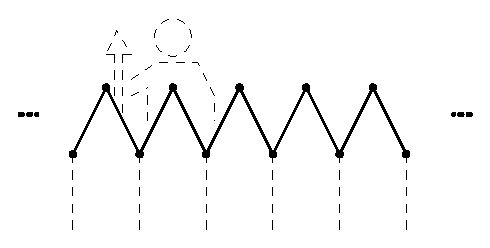
\includegraphics[width=100mm]{img/palisada.eps}
\[\xymatrix@R=7pt@C=14pt{& &-3\ \ar@{-}[ddl]\ar@{-}[ddr] & & -1\ \ar@{-}[ddl]\ar@{-}[ddr] & & \ 1\ \ar@{-}[ddl]\ar@{-}[ddr] & & \ 3\ \ar@{-}[ddl]\ar@{-}[ddr] \\ \cdots & & & & & & & & & & \cdots\\
& -4\  & & -2\  & & \ 0\  & & \ 2\ & & \ 4\ }\]
\caption{Obustronnie nieskończona palisada, czyli $\mathcal{C}$-korozbieralny $\mathcal{C}$-rdzeń z~przykładu \ref{buildable_not_dismantlable}.}\label{fig-palisada}
\end{figure}


\begin{problem}\label{prob1}
Czy $\mathcal{R}$-rozbieralność $X$~do~$A$, gdzie $\mathcal{R}\in\{\mathcal{I},\mathcal{C}\}$, implikuje \mbox{$\mathcal{R}$-korozbieralność} $X$~z~$A$~dla dowolnej pary przestrzeni Aleksandrowa $(X,A)$?
\end{problem}

Interesującą klasą częściowych porządków, zawierającą klasę porządków bez promieni, są rozważane na przykład przez Farleya \cite{Farley97} porządki bez nieskończonych łańcuchów i~\textit{jednostronnie nieskończonych palisad} (tj.~podzbiorów izomorficznych ze zbiorem $\mN$~z porządkiem zadanym jak w~przykładzie \ref{buildable_not_dismantlable} bądź z~porządkiem do niego dualnym). Naturalne wydaje się pytanie o~odpowiednik twierdzenia \ref{build_if_dism} dla tej klasy.

\begin{problem}\label{prob2}
Niech $X$~będzie przestrzenią Aleksandrowa nie zawierającą nieskończonych łańcuchów i~nieskończonych palisad, zaś $A$~jej podzbiorem. Czy $X\dism A$ wtedy i~tylko wtedy, gdy $A\codism X$?
\end{problem}

Niech $\left(s_{\phi+1,\phi}\colon A_{\phi+1}\to A_{\phi}\right)_{\phi<\beta}$ będzie ciągiem $\mathcal{R}$-korozbierającym przestrzeń $X$~z~$A$. Dla każdej liczby porządkowej $\psi\leq \beta$ określimy retrakcję $\revcomp\left(s_{\phi}\right)_{\psi\leq \phi<\beta}\colon X\to A_\psi$ zwaną \textit{nieskończonym złożeniem wstecz}\index{nieskonzzzczone zlzzzozzzzenie@nieskończone złożenie!wstecz}\nomenclature[7r]{$\revcomp\left(s_{\phi}\right)_{\psi\leq\phi<\beta}$}{nieskończone złożenie wstecz ciągu retrakcji $\left(s_{\phi}\colon X_{\phi+1}\to X_\phi\right)_{\psi\leq\phi<\beta}$} elementów ciągu $\left(s_{\phi+1,\phi}\right)_{\psi\leq \phi<\beta}$. W~tym celu zdefiniujemy najpierw pomocniczą \textit{funkcję skoku}\index{odwzorowanie!skoku}\index{funkcja!skoku}\label{def-nieskonczone_zlozenie_korozbierajacego_ciagu}
 $\s\left(s_{\phi+1,\phi}\right)_{\phi<\beta}\colon X\to X$\nomenclature[7ra]{$\s\left(s_{\phi}\right)_{\phi<\beta}$}{funkcja skoku związana z~ciągiem retrakcji $\left(s_{\phi}\colon X_{\phi+1}\to X_\phi\right)_{\phi<\beta}$}. Dla $x\in A$ niech $\s\left(s_{\phi+1,\phi}\right)_{\phi<\beta}(x)=x$. Natomiast dla $x\not\in A$ istnieje największa liczba porządkowa $0\leq \phi_x<\beta$ taka, że $x\not\in A_{\phi_x}$; przyjmujemy $\s\left(s_{\phi+1,\phi}\right)_{\phi<\beta}(x)=s_{\phi_{x}+1,\phi_{x}}(x)$. 

Dla $\psi\leq\beta$ oraz $x\in X$ niech \[\revcomp\left(s_{\phi+1,\phi}\right)_{\psi\leq \phi<\beta}(x)=\left(\s\left(s_{\phi+1,\phi}\right)_{\phi<\beta}(x)\right)^{n^x_\psi}(x),\] gdzie \[n_\psi^x=\min\left\{n\in\mN:\left(\s\left(s_{\phi+1,\phi}\right)_{\phi<\beta}(x)\right)^n(x)\in A_\psi\right\}.\]

\begin{lem}\label{lem-iteracje_s_na_x_tworza_skonczony_zbior}
Niech $(X,A)$~będzie parą przestrzeni Aleksandrowa, zaś $\left(s_{\phi+1,\phi}\colon A_{\phi+1}\to A_{\phi}\right)_{\phi<\beta}$ ciągiem $\mathcal{R}$-korozbierającym przestrzeń $X$~z~$A$. Wówczas dla każdego elementu $x\in X$ zbiór \[\left\{\left(\s\left(s_{\phi+1,\phi}\right)_{\phi<\beta}(x)\right)^n(x):n\in\mN\right\}=\left\{\revcomp\left(s_{\phi+1,\phi}\right)_{\psi\leq \phi<\beta}(x):\psi\leq\beta \right\}\] jest skończony.
\end{lem}
\begin{proof}
Dla elementu $x\in X$ niech \[\phi(x)=\min\left\{0\leq \phi<\beta:x\in A_{\phi}\right\}.\] 
Zauważmy, że dla każdego $x\in X\smallsetminus A$ zachodzi nierówność \[\phi\left(\s\left(s_{\phi+1,\phi}\right)_{\phi<\beta}(x)\right)< \phi(x).\] Zbiór \[\left\{\phi\left(\left(\s\left(s_{\phi+1,\phi}\right)_{\phi<\beta}\right)^n(x)\right):n\in\mN\right\}\] jest dobrze uporządkowany, więc nie zawiera nieskończonego łańcucha zstępującego; musi zatem być skończony. Ponadto $\s\left(s_{\phi+1,\phi}\right)_{\phi<\beta}\big|_A=\id_A$. Wobec tego skończony jest również zbiór \[\left\{\left(\s\left(s_{\phi+1,\phi}\right)_{\phi<\beta}(x)\right)^n(x):n\in\mN\right\}.\qedhere\]
\end{proof}

Następujący wynik jest dotyczącym korozbieralności odpowiednikiem lematu \ref{lem-Irozbieralny-wtw-Crozbieralny}.
\begin{lem}\label{lem-Ckorozb_wtw_Ikorozb}
Niech $(X,A)$~będzie parą przestrzeni Aleksandrowa bez nieskończonych łańcuchów. Następujące warunki są równoważne:
\begin{compactitem}
\item[1)] $A\codism X$;
\item[2)] przestrzeń $X$~jest $(\mathcal{U}\cup\mathcal{D})$-korozbieralna z~$A$;
\item[3)] przestrzeń $X$~jest $\mathcal{I}$-korozbieralna z~$A$;
\end{compactitem}
\end{lem}
\begin{proof}
1)$\implies$2)\,: Jak w~dowodzie lematu \ref{lem-Irozbieralny-wtw-Crozbieralny} każdą $\mathcal{C}$-retrakcję z~ciągu \mbox{$\mathcal{C}$-korozbierającego} $X$~z~$A$~możemy przedstawić jako złożenie dwóch \mbox{$(\mathcal{U}\cup\mathcal{D})$-retrakcji}.

2)$\implies$3)\,: Rozważmy $\mathcal{D}$-retrakcję $r\colon Y\to r(Y)$ określoną na przestrzeni Aleksandrowa bez nieskończonych łańcuchów $Y$ i~różną od $\id_{Y}$. Zbiór \[B=\{y\in Y:r(y)\not=y\}\] jest niepusty, zatem $\min(B)\not=\emptyset$, gdyż porządek $Y$~jest dobrze ufundowany. Jeżeli $y_0\in\min(B)$, to ponieważ $r(y_0)<y_0$ oraz $r(y)=y$ dla wszystkich $y<y_0$, punkt $y_0$~jest nieredukowalny nad punktem $r(y_0)$. Istnieje więc \mbox{$\mathcal{I}$-retrakcja} $r_0\colon r(Y)\cup\{y_0\}\to r(Y)$~przeprowadzająca punkt $y_0$ na $r(y_0)$. Ponadto funkcja $r'\colon Y\to r(Y)\cup\{y_0\}$ zadana dla $y\in Y$ wzorem \[r'(y)=\begin{cases}r(y) & \text{dla } y\not=y_0,\\y_0 & \text{dla } y=y_0\end{cases}\] jest $\mathcal{D}$-retrakcją. Korzystając z~tej obserwacji nietrudno udowodnić za pomocą indukcji pozaskończonej, że przestrzeń $Y$~jest \mbox{$\mathcal{I}$-korozbieralna} z~$r(Y)$. Stosując to rozumowanie (oraz rozumowanie dualne) do retrakcji z~ciągu \mbox{$(\mathcal{U}\cup\mathcal{D})$-korozbierającego} $X$~z~$A$~wykazuje się \mbox{$\mathcal{I}$-korozbieralność} $X$~z~$A$.

3)$\implies$1)\,: Oczywiste, gdyż $\mathcal{I}\subseteq \mathcal{C}$.
\end{proof}

Podobnie jak w~przypadku lematu \ref{lem-Irozbieralny-wtw-Crozbieralny}, dowód równoważności warunków 1)~i~2)~lematu \ref{lem-Ckorozb_wtw_Ikorozb} oraz wynikania warunku 1)~z~warunku 3)~nie wymaga założenia o~braku nieskończonych łańcuchów w~$X$.

%---------------------------------------------------------------
%---------------------------------------------------------------
%---------------------------------------------------------------



\subsection{Klasyfikacja typów homotopijnych przestrzeni Aleksandrowa bez promieni}
W~niniejszej sekcji udowodnimy twierdzenie rozszerzające podaną przez Stonga ,,klasyfikację'' typów homotopijnych skończonych przestrzeni topologicznych (twierdzenie \ref{tw-stonga}) na przestrzenie Aleksandrowa bez promieni.

Użyteczne okaże się przy tym pojęcie rzędu grafu prostego bez promieni, zdefiniowane przez Schmidta \cite{Schmidt83}. Przypomnimy je oraz niektóre jego własności w~oparciu o~popularyzujące to pojęcie opracowanie autorstwa Halina \cite{Halin98}.

Dla każdej liczby porządkowej $\phi$~definiujemy indukcyjnie pewną klasę grafów prostych $\mathcal{RL}(\phi)$ \cite[Definition 3.1]{Halin98} w~następujący sposób:
\begin{compactitem}
\item[---] $\mathcal{RL}(0)$ jest klasą grafów skończonych,
\item[---] jeżeli $\phi>0$, to graf $H$~należy do $\mathcal{RL}(\phi)$, jeśli istnieje skończony zbiór wierzchołków $F\subseteq H$ taki, że każda spójna składowa grafu $H-F$ należy do $\mathcal{RL}(\psi)$ dla pewnego $\psi<\phi$.
\end{compactitem}
Przez $\mathcal{RL}$~oznaczmy sumę wszystkich klas $\mathcal{RL}(\phi)$. Okazuje się, że graf $H$~należy do $\mathcal{RL}$~dokładnie wtedy, gdy jest grafem bez promieni \cite[Proposition 3.2]{Halin98}. Dla $H\in \mathcal{RL}$ \textit{rzędem}\index{rzazzzd grafu bez promieni@rząd grafu bez promieni} grafu $H$, oznaczanym symbolem $\ord(H)$\nomenclature[2k]{$\ord(G)$}{rząd grafu prostego bez promieni $G$}, nazywamy najmniejszą liczbę porządkową $\phi$~taką, że $H\in \mathcal{RL}(\phi)$. 

Dla nieskończonego grafu bez promieni $H$~istnieje najmniejszy (w~sensie inkluzji) skończony podzbiór $F$~zbioru wierzchołków tego grafu taki, że dla każdej spójnej składowej $D$~grafu $H-F$ zachodzi nierówność $\ord(D)<\ord(H)$ \cite[Lemma 3.11]{Halin98}. Zbiór $F$~o~powyższej własności nazywamy \textit{jądrem}\index{jazzzdro@jądro!grafu bez promieni} grafu $H$ \cite[Definition 3.12]{Halin98}~i~piszemy $\ker(H)=F$.\nomenclature[2j]{$\ker(G)$}{jądro grafu prostego bez promieni $G$} 

Dla częściowego porządku $P$~przyjmujemy oznaczenia $\ord(P)=\ord(\Comp(P))$ oraz $\ker(P)=\ker(\Comp(P))$.

Poniższe twierdzenie stanowi kluczową innowację bieżącego rozdziału w~stosunku do prac autora \cite{Kukiela10a,Kukiela10} i~pozwala na uogólnienie ich głównych wyników na wszystkie przestrzenie Aleksandrowa bez promieni. W~cytowanych pracach podobne twierdzenie \cite[wniosek III.2.2]{Kukiela10a}, \cite[Proposition 4.4]{Kukiela10} udowodnione zostało innymi metodami, ale jedynie dla przeliczalnych przestrzeni Aleksandrowa bez promieni oraz dla przestrzeni Aleksandrowa (dowolnej mocy), w~których wszystkie ścieżki proste są ograniczonej długości.

\begin{tw}\label{mocny_retrakt}
Jeśli $(X,A)$ jest $\Gamma$-parą przestrzeni Aleksandrowa bez promieni, to istnieje $\mathcal{C}$-rdzeń $(X^C,A)\subseteq (X,A)$, będący ekwiwariantnym mocnym retraktem deformacyjnym pary $(X,A)$ i~taki, że $X\dism^\Gamma X^C$.
\end{tw}
\begin{proof}
Przeprowadzimy indukcję ze względu na $\ord(X)$. %~oraz $\moc{\ker(X)}$. 

Załóżmy najpierw, że $\ord(X)=0$, co oznacza, że przestrzeń $X$~jest skończona. Jeśli $X=A$, nie mamy czego dowodzić. Załóżmy, że twierdzenie jest prawdziwe dla wszystkich par $(Y,A)$ takich, że $A\subseteq Y\subsetneq X$. Jeżeli $U_{(X,A)}=D_{(X,A)}=\id_X$, to wobec~lematu \ref{ciag_standardowy_staly_to_mamy_rdzen} para $(X,A)$ jest $\mathcal{C}$-rdzeniem. Jeśli jedna z~retrakcji $D_{(X,A)}$, $U_{(X,A)}$ nie jest tożsamościowa, oznaczmy ją przez $r\colon X\to r(X)$. Funkcja $r$~jest ekwiwariantną $\mathcal{C}$-retrakcją (lemat \ref{standardowy_jest_g}), więc \mbox{$X\dism^\Gamma r(X)$}. Na podstawie stwierdzenia \ref{stw-porownywalne_sa_homotopijne} istnieje homotopia $i\circ r\simeq \id_X\ \operatorname{rel} A$, gdzie $i\colon r(X)\hookrightarrow X$ jest włożeniem; nietrudno spostrzec, że jest ona ekwiwariantna. Ponieważ $r(X)\subsetneq X$, teza wynika z~założenia indukcyjnego.

Załóżmy, że $\ord(X)>0$ oraz twierdzenie jest prawdziwe dla każdej \mbox{$\Gamma$-pary} $(Y,B)$ przestrzeni Aleksandrowa bez promieni takiej, że $\ord(Y)<\ord(X)$. 

Przez $\left\{\hat{X}_i\right\}_{i\in I}$ oznaczmy indeksowaną rodzinę wszystkich składowych spójności przestrzeni $X\smallsetminus \ker(X)$. Zauważmy, że $\ord\left(\hat{X}_i\right)<\ord(X)$ dla każdego indeksu $i\in I$. Niech $A'=A\cup \ker(X)$; dla każdego indeksu $i\in I$ przyjmijmy oznaczenia $X_i=\hat{X}_i\cup \ker(X)$ oraz $A_i=X_i\cap A'$. Z~założenia indukcyjnego dla każdej z~przestrzeni $(X_i,A_i)$ istnieją zawarty w~niej $\mathcal{C}$-rdzeń $\left(X_i^C,A_i\right)$, liczba porządkowa $\alpha_i$, ciąg \[\left(r_i^{\phi,\phi+1}\colon X_i^{\phi}\to X_i^{\phi+1}\right)_{\phi<\alpha_i}\] retrakcji $\mcC$-rozbierający $X_i$~do~$X_i^C$ oraz mocna retrakcja deformacyjna $R_i\colon (X_i,A_i)\to \left(X_i^C,A_i\right)$.

Przyjmijmy oznaczenie $X^*=\bigcup_{i\in I}X_i^C$. Ponieważ $X_i\cap X_j=\ker(X)$ dla $i\not= j$ oraz $\bigcup_{i\in I}X_i=X$, funkcja $R=\bigcup_{i\in I} R_i\colon \left(X,A'\right)\to \left(X^*,A'\right)$ jest mocną retrakcją deformacyjną, a~ponadto para $(X^*,A')$ jest $\mathcal{C}$-rdzeniem. Niech \mbox{$\alpha=\max\{\alpha_i:i\in I\}$}. Dla $\alpha_i \leq \phi<\alpha$ przyjmijmy $r_i^{\phi,\phi+1}=\id_{X_i^{\alpha_i}}$. Wówczas \[\left(\bigcup_{i\in I}r_i^{\phi,\phi+1}\colon \bigcup_{i\in I}X_i^{\phi}\to \bigcup_{i\in I}X_i^{\phi+1}\right)_{\phi<\alpha}\] jest ciągiem $\mathcal{C}$-rozbierającym $X$~do zbioru $X^*$.

Co więcej, możemy retrakcje $R_i$~oraz $r_i^{\phi,\phi+1}$ dla $i\in I$, $\phi<\alpha_i$, dobrać tak, aby retrakcja deformacyjna $R$~oraz retrakcje~$\bigcup_{i\in I}r_i^{\phi,\phi+1}$ były zgodne z~działaniem grupy~$\Gamma$.

Przeprowadzimy indukcję ze względu na liczbę elementów zbioru $\ker(X)$. Jeśli $\moc{\ker(X)}=0$, to $A=A'$, a~zatem para $(X^*,A')=(X^*,A)$ jest $\mathcal{C}$-rdzeniem będącym mocnym retraktem deformacyjnym pary $(X,A)$, czyli teza twierdzenia zachodzi. 

Załóżmy, że twierdzenie jest prawdziwe dla wszystkich par $(Y,B)$ przestrzeni Aleksandrowa bez promieni o~tej własności, że $\ord(Y)=\ord(X)$ oraz $\moc{\ker(Y)}<\moc{\ker(X)}$. Rozważmy $\Gamma$-retrakcje $U_{(X^*,A)}$, $D_{(X^*,A)}$. Jeśli są one odwzorowaniami identycznościowymi, to $(X^*,A)$ jest $\mathcal{C}$-rdzeniem (lemat \ref{ciag_standardowy_staly_to_mamy_rdzen}), zaś $R$~szukaną retrakcją deformacyjną. Jeżeli natomiast jedno z~tych odwzorowań, oznaczmy je przez $\rho$, nie jest tożsamościowe, to istnieje punkt \mbox{$x\in X^*\smallsetminus A$} nieredukowalny w~$X^*$~i~taki, że $\rho(x)\not=x$. Ponieważ para $\left(X^*,A'\right)$ jest \mbox{$\mathcal{C}$-rdzeniem}, punkt \mbox{$x\not\in X^*\smallsetminus A'$}, a~zatem $x\in A'\smallsetminus A\subseteq \ker(X)$. Wobec tego $\moc{\ker\left(\rho\left(X^*\right)\right)}<\moc{\ker(X)}$. Z~założenia indukcyjnego istnieją $\mathcal{C}$-rdzeń $\left(X^C,A\right)$~oraz ekwiwariantna mocna retrakcja deformacyjna $S\colon \left(\rho\left(X^*\right),A\right)\to \left(X^C,A\right)$. Odwzorowanie \mbox{$(s\circ \rho\circ R)\colon (X,A)\to \left(X^C,A\right)$} jest ekwiwariantną mocną retrakcją deformacyjną. W~podobny sposób znajdujemy ciąg $\Gamma$-retrakcji $\mathcal{C}$-rozbierający $X$~do~$X^C$.
\end{proof}

Sama $\mathcal{C}$-rozbieralność przestrzeni Aleksandrowa bez promieni do $\mathcal{C}$-rdzenia jednoznacznego z~dokładnością do izomorfizmu jest dobrze znanym faktem \cite[Corollary 3.15]{Schroder99}.  Ważne w~twierdzeniu \ref{mocny_retrakt} jest istnienie mocnej retrakcji deformacyjnej na rdzeń.

Mówimy, że para przestrzeni Aleksandrowa $(X,A)$ jest \textit{lokalnie rdzeniem}\index{czezzzszzzciowy porzazzzdek@częściowy porządek!lokalnie rdzenzzz@lokalnie rdzeń}\index{rdzenzzz@rdzeń!(czezzzszzzciowy porzazzzdek)@(częściowy porządek)!lokalnie rdzenzzz@lokalnie rdzeń}, o~ile dla każdego $x\in X$ istnieje skończony zbiór $\lc_X(x)\subseteq X$\nomenclature[7o]{$\lc_X(x)$}{struktura lokalnego rdzenia wokół elementu $x$~zbioru częściowo uporządkowanego $X$} taki, że $x\in\lc_X(x)$ oraz spełnione są następujące warunki:
\begin{compactitem}
\item[---] jeśli $y\in\lc_X(x)\smallsetminus A$ oraz $y\not\in\min(X)$, to $\moc{\lc_X(x)\cap\max(y\mathord{\downarrow}_X\smallsetminus\{y\})}\geqslant 2$,
\item[---] jeśli $y\in\lc_X(x)\smallsetminus A$ oraz $y\not\in\max(X)$, to $\moc{\lc_X(x)\cap\min(y\mathord{\uparrow}_X\smallsetminus\{y\})}\geqslant 2$. 
\end{compactitem}

Dowody poniższych dwóch faktów przebiegają tak samo jak dowody cytowanych przy nich twierdzeń, dotyczących szczególnego przypadku, gdy zbiór $A$~jest pusty lub jednoelementowy.

\begin{tw}[{{\cite[twierdzenie III.2.3]{Kukiela10a}, \cite[Theorem 4.6]{Kukiela10}}}]\label{o_lokalnych_rdzeniach}Jeśli para przestrzeni Aleksandrowa $(X,A)$ jest lokalnie rdzeniem, to nie istnieje ciągłe odwzorowanie $f\colon (X,A)\to (X,A)$ takie, że $f\simeq \id_X \operatorname{rel} A$ oraz $f\not=\id_X$.
\end{tw}

\begin{stw}[{{\cite[twierdzenie III.2.5]{Kukiela10a}, \cite[Proposition 4.8]{Kukiela10}}}]\label{fp_rdzenie_sa_lokalne}
Jeśli para $(X,A)$ przestrzeni Aleksandrowa bez promieni jest $\mathcal{C}$-rdzeniem, to $(X,A)$ jest lokalnie rdzeniem.
\end{stw}

Z~twierdzenia \ref{o_lokalnych_rdzeniach} wynika, że jeśli para $(X,A)$ przestrzeni Aleksandrowa jest lokalnie rdzeniem, to jest $\mathcal{C}$-rdzeniem. Otrzymujemy z~niego natychmiast również  następujący wniosek.
\begin{wn}\label{lokalne_sa_dobre}
Jeśli pary przestrzeni Aleksandrowa $(X,A)$, $(Y,B)$ są lokalnie rdzeniami, zaś $f\colon (X,A)\to (Y,B)$, $g\colon (Y,B)\to (X,A)$ są ciągłymi odwzorwaniami takimi, że $g\circ f\simeq \id_X \operatorname{rel} A$ oraz $f\circ g\simeq \id_Y \operatorname{rel} B$, to $f,g$ są wzajemnie odwrotnymi homeomorfizmami.
\end{wn}

Poniższe twierdzenie, będące głównym wynikiem rozdziału, uogólnia na przestrzenie Aleksandrowa bez promieni podaną przez Stonga klasyfikację typów homotopijnych skończonych przestrzeni topologicznych (twierdzenie \ref{tw-stonga}) oraz wyniki uzyskane przez autora \cite{Kukiela10a,Kukiela10}.

\begin{tw}\label{wniosek_klasyfikacyjny}
Jeśli $X$, $Y$ są $\Gamma$-przestrzeniami Aleksandrowa bez promieni, to istnieją $\mathcal{C}$-rdzenie $X^C$, $Y^C$ będące ich ekwiwariantnymi mocnymi retraktami deformacyjnymi i~takie, że $X\dism^\Gamma X^C$ oraz $Y\dism^\Gamma Y^C$. Przestrzeń $X$~jest $\Gamma$-homotopijnie równoważna przestrzeni $Y$~wtedy i~tylko wtedy, gdy rdzenie $X^C$, $Y^C$ są $\Gamma$-homeomorficzne. 
\end{tw}
\begin{proof}
O~istnieniu $\mathcal{C}$-rdzeni $X^C$, $Y^C$~będących ekwiwariantnymi mocnymi retraktami deformacyjnymi $X$, $Y$~mówi twierdzenie \ref{mocny_retrakt}.

Ponieważ $X\simeq X^C$ oraz $Y\simeq Y^C$ w~sposób ekwiwariantny, z~istnienia \mbox{$\Gamma$-homeomorfizmu} $X^C\approx Y^C$ wynika $\Gamma$-homotopijna równoważność przestrzeni $X$, $Y$. 

Z~drugiej strony, istnienie $\Gamma$-homotopijnej równoważności przestrzeni $X$~oraz $Y$~implikuje istnienie $\Gamma$-homotopijnej równoważności pomiędzy $X^C$~a~$Y^C$. Wobec stwierdzenia \ref{fp_rdzenie_sa_lokalne} przestrzenie $X^C$, $Y^C$ są lokalnie rdzeniami. Zastosowanie wniosku \ref{lokalne_sa_dobre} kończy dowód.
\end{proof}

%---------------------------------------------------------------
%---------------------------------------------------------------
%---------------------------------------------------------------


\subsection{Wnioski z~twierdzenia klasyfikacyjnego}
Odnotujmy kilka wniosków z~rozważań poprzedniej sekcji. Rozpoczynamy od analogicznej jak w~przypadku skończonych przestrzeni topologicznych (por.~\cite[Corollary 4.9]{Barmak12}) charakteryzacji mocnych retraktów deformacyjnych przestrzeni Aleksandrowa bez promieni.

\begin{wn}\label{wn-charakteryzacja-mocnych-retraktow-deformacyjnych}
Niech $(X,A)$~będzie $\Gamma$-parą przestrzeni Aleksandrowa bez promieni. Następujące warunki są równoważne:
\begin{compactenum}
\item[1)] $A$~jest ekwiwariantnym mocnym retraktem deformacyjnym $X$;
\item[2)] $X\dism^{\Gamma} A$;
\item[3)] $A\codism^\Gamma X$.
\end{compactenum}
\end{wn}
\begin{proof}
Równoważność warunków 2) oraz 3) została wykazana w~twierdzeniu \ref{build_if_dism}. Wystarczy zatem udowodnić, że równoważne są warunki 1) i~2).

Zgodnie z~twierdzeniem \ref{mocny_retrakt} $X\dism^\Gamma X^C$ dla pewnej zawierającej zbiór $A$~podprzestrzeni $X^C\subseteq X$ takiej, że para $\left(X^C,A\right)$ jest $\mathcal{C}$-rdzeniem oraz istnieje ekwiwariantna mocna retrakcja deformacyjna $T\colon X\to X^C$.

Załóżmy, że $A$~jest ekwiwariantnym mocnym retraktem deformacyjnym $X$. Wówczas $(X^C,A)\simeq (A,A)$. Ponieważ pary $\left(X^C,A\right)$, $(A,A)$ są $\mathcal{C}$-rdzeniami, wobec stwierdzenia \ref{fp_rdzenie_sa_lokalne} oraz wniosku \ref{lokalne_sa_dobre} oznacza to, że $X^C=A$. Ale, jak zauważyliśmy, $X\dism^\Gamma X^C$.

Załóżmy, że $X\dism^\Gamma A$. Ustalmy liczbę porządkową $\alpha$~oraz \mbox{$\mathcal{C}$-rozbierający} $X$~do $A$~ciąg $\left(r_{\phi,\phi+1}\colon X_\phi\to X_{\phi+1}\right)_{\phi<\alpha}$ ekwiwariantnych retrakcji. Przyjmijmy oznaczenie $R=\infcomp\left(r_{\phi,\phi+1}\right)_{0\leq\phi<\alpha}\colon X\to A$. Wobec lematu \ref{lem-schroder_lemma} zachodzi równość $T\circ R\big|_{X^C}=\id_{X^C}$. Ale $R(X)=A$, zaś $T\big|_A=\id_A$, zatem $(T\circ R)\left(X^C\right)= A$. Stąd $X^C=A$.
\end{proof}
W~szczególności przestrzeń Aleksandrowa bez promieni jest ściągalna wtedy i~tylko wtedy, gdy pewien jej punkt jest jej mocnym retraktem deformacyjnym, co~jest z~kolei równoważne $\mathcal{C}$-rozbieralności do tego punktu. Częściowo odpowiada to na pytanie postawione przez autora \cite[Problem 5]{Kukiela10a}, \cite[Question 4]{Kukiela10}.
Nie jest jednak prawdą, że dowolny punkt ściągalnej przestrzeni Aleksandrowa bez promieni (a~nawet ściągalnej skończonej przestrzeni topologicznej) jest jej mocnym retraktem deformacyjnym. Kontrprzykład przedstawia rysunek \ref{fig-punkt_nie_bedacy_mocnym_retraktem_deformacyjnym}.

\begin{figure}[h]
\[
\xymatrix{\bullet\ar@{-}[d]\ar@{-}[drr] & \bullet\ar@{-}[dl]\ar@{-}[drr] & \bullet\ar@{-}[d]\ar@{-}[dr]\\
\!\!\!a\ \bullet\ar@{-}[drr] & & \bullet\ar@{-}[d]\ar@{-}[dr] & \bullet\ar@{-}[d]\ar@{-}[dl]\\
& & \bullet & \bullet}
\]
\caption{Diagram Hassego ściągalnej, skończonej przestrzeni topologicznej $X$~z~punktem wyróżnionym $a$~o~tej~własności, że $(X,\{a\})$ jest $\mcC$-rdzeniem, a~zatem przestrzeń $X$~nie jest $\mcC$-rozbieralna do $a$.}\label{fig-punkt_nie_bedacy_mocnym_retraktem_deformacyjnym}
\end{figure}

Wniosek \ref{wn-charakteryzacja-mocnych-retraktow-deformacyjnych} odpowiada również twierdząco na pytanie o~homotopijną równoważność przestrzeni Aleksandrowa bez promieni z~podzbiorem, do którego jest ona $\mcC$-rozbieralna~\cite[Problem 4]{Kukiela10a}, \cite[Question 3]{Kukiela10}.

Warto wspomnieć, że prawdziwe jest niniejsze stwierdzenie, będące uogólnieniem wyniku Stonga \cite{Stong84}. Jego dowód przebiega analogicznie jak dowód cytowanego przy nim słabszego odpowiednika z~pracy autora~\cite{Kukiela10}.
\begin{stw}[por.~{\cite[stwierdzenie III.3.4]{Kukiela10}}]
Załóżmy, że $X$, $Y$~są \mbox{$\Gamma$-przestrzeniami} Aleksandrowa bez promieni. Wówczas $\Gamma$-odwzorowanie $f:X\to Y$ jest $\Gamma$-homotopijną równoważnością wtedy i~tylko wtedy, gdy $f$~jest homotopijną równoważnością.
\end{stw}

Skupialiśmy się dotąd głównie na podobieństwach między skończonymi przestrzeniami topologicznymi a~przestrzeniami Aleksandrowa bez promieni. Pewną interesującą różnicę pomiędzy tymi klasami zauważyć można przyglądając się pojęciu homotopijnej dominacji. Przypomnijmy, że przestrzeń topologiczna $X$~\textit{homotopijnie dominuje}\index{homotopijna dominacja} nad przestrzenią topologiczną $Y$, co zapisujemy przez $X\geq_H Y$, o~ile istnieją ciągłe odwzorowania $f\colon X\to Y$, $g\colon Y\to X$ takie, że $f\circ g\simeq \id_Y$. Można udowodnić \cite[stwierdzenie III.3.1]{Kukiela10a}, że jeśli dla skończonych przestrzeni topologicznych $X$, $Y$~zachodzą homotopijne dominacje $X\geq_H Y$ oraz $Y\geq_H X$, to przestrzenie te są homotopijnie równoważne. Nie jest to prawdą dla dowolnych przestrzeni Aleksandrowa (patrz \cite[przykład III.3.2]{Kukiela10a}). Niżej wykazujemy, że fakt ten nie uogólnia się nawet na przestrzenie Aleksandrowa bez promieni. (Obserwacja ta wydaje się mieć bliski związek z~rozważaniami dotyczącymi tzw.~odwracalnych i~bijektywnie związanych częściowych porządków \cite{Kukiela09,Kukiela13a}.)

\begin{ex}
Dla $n\in\mN$ symbolem $A_n$~oznaczmy antyłańcuch o~$n$~elementach. Niech $K_{n,n}=A_n\oplus A_n$. Dla każdego $n\in\mN$ wybierzmy punkt wyróżniony $x_n\in \min(K_{n,n})$. Rozważmy przestrzenie ilorazowe \[X=\left(\coprod_{n\geq 1} K_{2n,2n}\right)\big/\{x_{2n}:n\in\mN\},\quad Y=\left(\coprod_{n\geq 1} K_{2n+1,2n+1}\right)\big/\{x_{2n+1}:n\in\mN\}.\] Łatwo zauważyć, że są one przestrzeniami Aleksandrowa bez promieni oraz \mbox{$\mathcal{C}$-rdzeniami}. Przestrzenie te nie są izomorficzne, a~zatem wobec twierdzenia \ref{wniosek_klasyfikacyjny} nie są homotopijnie równoważne. Widać jednak, że przestrzeń $X$~jest homeomorficzna pewnemu retraktowi przestrzeni $Y$, i~odwrotnie, $Y$~jest homeomorficzna retraktowi $X$. Zatem $X\geq_H Y$ oraz $Y\geq_H X$. 
\end{ex}


%---------------------------------------------------------------
%---------------------------------------------------------------
%---------------------------------------------------------------


\subsection{H-przestrzenie i~ko-H-przestrzenie Aleksandrowa bez promieni}
Przypomnijmy, że \textit{H-przestrzenią}\index{Hprzestrzenzzz@H-przestrzeń} nazywamy trójkę $(X,p,\mu)$ składającą się z~przestrzeni topologicznej $X$, jej wyróżnionego punktu $p\in X$ oraz ciągłego, zachowującego punkty wyróżnione odwzorowania $\mu:X\times X\to X$ o~tej własności, że diagram \[\xymatrix@C=60pt@R=40pt{X\ar[dr]_{\id_X}\ar[r]^{(p,\id_X)} & X\times X\ar[d]^{\mu} & X\ar[dl]^{\id_X}\ar[l]_{(\id_X,p)} \\ & X}\]
jest przemienny z~dokładnością do homotopii zachowującej punkty wyróżnione. Przez $p$~oznaczyliśmy w~powyższym diagramie odwzorowanie stałe.

Jeśli istnieje homotopijna równoważność $(X,p)\simeq (Y,q)$, to struktura \mbox{H-przestrzeni} na $X$ indukuje strukturę \mbox{H-przestrzeni} na $Y$ \cite[Theorem 1.5.4]{Spanier81}. Ponadto, jeśli przestrzeń $(X,p)$ jest ściągalna, to można na niej wprowadzić trywialne działanie $\mu:X\times X\to X$ takie, że $(X,p,\mu)$ jest H-przestrzenią: wystarczy przyjąć $\mu(x,y)=p$ dla wszystkich $x,y\in X$.

Stong~\cite{Stong66} udowodnił, że każda spójna, skończona H-przestrzeń jest ściągalna. Jego dowód przenosi się na przestrzenie Aleksandrowa bez promieni przy wykorzystaniu wyników niniejszej rozprawy prawie bez zmian. (W~dowodzie \cite[Proposition 13]{Stong66} należy jedynie zauważyć, że sumy zbiorów $D_r, D_r'$ zawierają nieskończone ścieżki proste.) Ponieważ jest on dość długi, nie przytaczamy go, poniższe twierdzenie pozostawiając bez dowodu.

\begin{stw}[por. {\cite[Section 5]{Stong66}}]\label{stw-stonga_o_h_przestrzeniach}
Niech $X$~będzie spójną przestrzenią Aleksandrowa bez promieni. Warunkiem koniecznym i~dostatecznym na to, by istniała struktura H-przestrzeni $(X,p,\mu)$ jest istnienie mocnej retrakcji deformacyjnej przestrzeni $X$~na przestrzeń jednoelementową $\{p\}$.
\end{stw}

Pojęciem dualnym do H-przestrzeni jest \textit{ko-H-przestrzeń}\index{ko-H-przestrzenzzz@ko-H-przestrzeń}, to jest trójka $(X,p,\eta)$ składająca się z~przestrzeni topologicznej $X$~z~punktem wyróżnionym $p\in X$ oraz ciągłego, zachowującego punkty wyróżnione odwzorowania $\eta\colon X\to X\vee X$ o~tej własności, 
że diagram
\[\xymatrix@C=60pt@R=40pt{X\ar@{<-}[dr]_{\id_X} & X\vee X\ar[l]_{\pi_1}\ar[r]^{\pi_2}\ar@{<-}[d]^{\eta} & X\ar@{<-}[dl]^{\id_X} \\ & X}\]
jest przemienny z~dokładnością do homotopii zachowującej punkty wyróżnione. W~powyższym diagramie $X\vee X=\{(x,y)\in X\times X: x=p \text{ lub } y=p\}$, zaś odwzorowania $\pi_1,\pi_2$ oznaczają rzuty odpowiednio na pierwszą i~drugą oś.

Podobnie jak ma to miejsce w~przypadku H-przestrzeni, jeżeli dana jest homotopijna równoważność $(X,p)\simeq (Y,q)$, to struktura ko-H-przestrzeni na $X$~wyznacza strukturę ko-H-przestrzeni na $Y$~\cite[Theorem 1.6.1]{Spanier81}. Jeśli przestrzeń $(X,p)$~jest ściągalna, to istnieje trywialne kodziałanie $\eta:X\to X\vee X$ (zadane dla wszystkich $x\in X$ wzorem $\eta(x)=(p, p)$) takie, że trójka $(X,p,\eta)$ jest \mbox{ko-H-przestrzenią}.

Helmstutler i~Vaughn \cite{Helmstutler10} wykazali, iż każda skończona ko-H-przestrzeń jest ściągalna. Podany przez nich prosty dowód zasadniczo różni się od dowodu wspomnianego wyżej wyniku Stonga, pomimo że same rezultaty wydają się dualne. Poniższe twierdzenie uogólnia twierdzenie Helmstutlera i~Vaughna na przestrzenie Aleksandrowa bez promieni.

\begin{stw}[por.~{\cite[Theorem 8]{Helmstutler10}}]\label{stw-helmsutlera-vaughna}
Niech $X$~będzie przestrzenią Aleksandrowa bez promieni. Warunkiem koniecznym i~dostatecznym na to, by istniała struktura ko-H-przestrzeni $(X,p,\eta)$ jest istnienie mocnej retrakcji deformacyjnej przestrzeni $X$~na przestrzeń jednoelementową $\{p\}$.
\end{stw}
\begin{proof}
Załóżmy, że istnieje struktura ko-H-przestrzeni $(X,p,\eta)$.
Wobec twierdzenia \ref{mocny_retrakt} istnieje $\mathcal{C}$-rdzeń $(X^C,p)$ będący mocnym retraktem deformacyjnym przestrzeni $(X,p)$. Na $X^C$ istnieje zatem struktura ko-H-przestrzeni $(X^C,p,\eta^C)$. Wykażemy, że $X^C=\{p\}$.

Ponieważ $\pi_1\circ \eta^C\simeq \id_{X^C}$ oraz $\pi_2\circ \eta^C \simeq \id_{X^C}$, z~twierdzeń \ref{o_lokalnych_rdzeniach}, \ref{fp_rdzenie_sa_lokalne} otrzymujemy $\pi_1\circ \eta^C=\id_{X^C}=\pi_2\circ \eta^C$.

Ustalmy $x\in X^C$. Wówczas $\eta^C(x)=(p,x')$ lub $\eta^C(x)=(x',p)$ dla pewnego elementu $x'\in X$. W~pierwszym przypadku mamy \[x=\id_{X^C}(x)=\left(\pi_1\circ\eta^C\right)(x)=p.\] Podobnie, w~drugim przypadku zachodzi równość $x=p$; stąd $X^C=\{p\}$.
\end{proof}

Powyższe twierdzenia oznaczają, że nie istnieje spójna, ale nieściągalna przestrzeń Aleksandrowa bez promieni $(X,p)$~taka, że dla każdej przestrzeni topologicznej z~punktem wyróżnionym $(Y,p)$ na  zbiorze klas homotopii $[(Y,q),(X,p)]$ lub na zbiorze $[(X,p),(Y,q)]$ istnieje naturalne działanie mające obustronny element neutralny \cite[Propositions 2.2.3, 2.2.9]{Arkowitz11}. W~szczególności na zbiorach tych nie istnieje naturalna struktura grupy.

Dodajmy, że Hardie, Vermeulen i~Witbooi \cite{Hardie02} rozpatrywali skończone przestrzenie topologiczne bedące ,,skończonymi modelami'' nietrywialnych \mbox{H-przestrzeni}, spełniające odpowiednio osłabione aksjomaty \mbox{H-przestrzeni}.

%---------------------------------------------------------------
%---------------------------------------------------------------
%---------------------------------------------------------------


\subsection{Słabsze formy rozbieralności przestrzeni Aleksandrowa}
Niech $\mathcal{R}$~będzie ustaloną klasą retrakcji w~kategorii przestrzeni Aleksandrowa. Przestrzeń Aleksandrowa nazywamy \textit{lokalnie $\mathcal{R}$-rozbieralną}\index{czezzzszzzciowy porzazzzdek@częściowy porządek!lokalnie rozbieralny}, jeżeli każdy jej skończony podzbiór zawiera się w~skończonym, $\mathcal{R}$-rozbieralnym podzbiorze tej przestrzeni. Podobną definicję w~przypadku grafów prostych podali np.~Hensel, Osajda i~Przytycki \cite{Hensel14}. Wyniki bieżącej sekcji zainspirowane są postawionym przez nich problemem \cite[Question 2.11]{Hensel14}, którego rozwiązanie (korzystające z~tych wyników) znajduje się w~rozdziale \ref{chap5}.

Wobec lematu \ref{lem-Irozbieralny-wtw-Crozbieralny} lokalna $\mathcal{I}$-rozbieralność jest równoważna lokalnej \mbox{$\mathcal{C}$-rozbieralności}. Ponieważ nie będziemy zajmować się lokalną \mbox{$\mathcal{R}$-rozbieralnością} dla $\mathcal{R}\not\in\{\mathcal{C},\mathcal{I}\}$, o~przestrzeni lokalnie \mbox{$\mathcal{C}$-rozbieralnej} mówimy krótko, że jest \textit{lokalnie rozbieralna}.

\begin{lem}\label{lem-rozb_to_slabo_rozb}
Niech $X$~będzie przestrzenią Aleksandrowa. Jeżeli $X\dism *$ lub $*\codism X$, to przestrzeń $X$~jest lokalnie rozbieralna.
\end{lem}
\begin{proof}
Ustalmy skończony podzbiór $D\subseteq X$.

Załóżmy, że $X\dism *$. Ustalmy liczbę porządkową $\alpha$ oraz $\mathcal{C}$-rozbierający $X$~do punktu ciąg $\left(r_{\phi,\phi+1}\right)_{\phi<\alpha}$. Zbiór \[\bigcup_{0\leq \psi<\alpha}\left(\infcomp\left(r_{\phi,\phi+1}\right)_{0\leq\phi<\psi}(D)\right)\] jest skończony (co wynika łatwo z~nieskończonej składalności ciągu \mbox{$\mathcal{C}$-rozbierającego}). Nietrudno spostrzec, że jest on \mbox{$\mathcal{C}$-rozbieralny}.

Podobnie, jeśli $*\codism X$ oraz $\left(s_{\phi+1,\phi}\right)_{\phi<\beta}$ jest, dla pewnej liczby porządkowej $\beta$, ciągiem $\mathcal{C}$-korozbierającym $X$~z~punktu, to~zbiór \[\bigcup_{0\leq \psi\leq \beta}\left(\revcomp\left(s_{\phi+1,\phi}\right)_{\psi\leq \phi<\beta}(D)\right)\] jest skończony (na podstawie lematu \ref{lem-iteracje_s_na_x_tworza_skonczony_zbior}) oraz $\mathcal{C}$-rozbieralny.
\end{proof}

\begin{figure}[h]
\[
\xymatrix@R=25pt@C=25pt{
&&		&		&		&		&		&		& 14\ar@{-}[d]\ar@{-}[dr]	& \widehat{14}\ar@{-}[d]\ar@{-}[dl]\\
&&		&		& 5\ar@{-}[d]\ar@{-}[dr]\ar@{-}[drr]	& \widehat{5}\ar@{-}[d]\ar@{-}[dl]\ar@{-}[drr]	&		&		& 13\ar@{-}[d]\ar@{-}[dr]\ar@{-}[dll]	& \widehat{13}\ar@{-}[d]\ar@{-}[dl]\ar@{-}[dll]\\
0\ar@{-}[drr] & \widehat{0}\ar@{-}[drr]	&	&		& 4\ar@{-}[d]\ar@{-}[dr]\ar@{-}[dll]\ar@{-}[drr]	& \widehat{4}\ar@{-}[d]\ar@{-}[dl]\ar@{-}[dll]\ar@{-}[drr]	& 6\ar@{-}[d]\ar@{-}[dr]	& \widehat{6}\ar@{-}[d]\ar@{-}[dl]	& 12\ar@{-}[d]\ar@{-}[dr]\ar@{-}[dll]	& \widehat{12}\ar@{-}[d]\ar@{-}[dl]\ar@{-}[dll] & \cdots\\
&&1\ar@{-}[d]\ar@{-}[dr]	& \widehat{1}\ar@{-}[d]\ar@{-}[dl]	& 3\ar@{-}[dll]\ar@{-}[drr]	& \widehat{3}\ar@{-}[dll]\ar@{-}[drr]	& 7\ar@{-}[d]\ar@{-}[dr]	& \widehat{7}\ar@{-}[d]\ar@{-}[dl]	& 11\ar@{-}[d]\ar@{-}[dr]\ar@{-}[dll]	& \widehat{11}\ar@{-}[d]\ar@{-}[dl]\ar@{-}[dll]\\
&&2		& \widehat{2}	& 		& 		& 8\ar@{-}[d]\ar@{-}[dr]	& \widehat{8}\ar@{-}[d]\ar@{-}[dl]	& 10\ar@{-}[dll]	& \widehat{10}\ar@{-}[dll]\\
&&		&		&		&		& 9	& \widehat{9}}
\]
\caption{Diagram Hassego lokalnie rozbieralnego częściowego porządku, który nie jest $\mathcal{C}$-rozbieralny ani $\mathcal{C}$-korozbieralny.}\label{slabo_rozb_ale_nie_rozb}
\end{figure}

\begin{ex}\label{ex-slabo_rozb_ale_nie_rozb}
Nie jest prawdą, że jeśli przestrzeń Aleksandrowa $X$~jest lokalnie rozbieralna, to $X\dism *$ lub $*\codism X$. Niech $X$~oznacza częściowy porządek, którego diagram Hassego przedstawiony jest na rysunku \ref{slabo_rozb_ale_nie_rozb}. Zauważmy, że jest on sumą wstępującego ciągu swoich skończonych, $\mathcal{I}$-rozbieralnych podzbiorów:
\[X=\bigcup_{n\in\mN} \left(\left\{m:0\leq m\leq a_n\right\}\cup \bigl\{\widehat{m}:0\leq m< a_n\bigr\}\right),\]
gdzie $a_0=0$ oraz $a_n=a_{n-1}+n+1$ dla $n\geq 1$. Przestrzeń $X$~jest zatem lokalnie rozbieralna. Nietrudno sprawdzić, że przestrzeń nie jest ona $\mathcal{C}$-rozbieralna ani $\mathcal{C}$-korozbieralna.
\end{ex}

\begin{comment}\begin{lem}\label{lem-retrakcje_zachowuja_slaba_rozbieralnosc}
Jeżeli przestrzeń Aleksandrowa~jest lokalnie rozbieralna, to każdy jej retrakt jest również lokalnie rozbieralny.
\end{lem}
\begin{proof}
Niech $X$~będzie lokalnie rozbieralną przestrzenią Aleksandrowa, zaś $r\colon X\to A$ zachowującą porządek retrakcją. Ustalmy skończony zbiór $D\subseteq A$. Ponieważ $A\subseteq X$, zbiór $D\subseteq X$. Istnieje zatem skończony, $\mathcal{I}$-rozbieralny zbiór $E\subseteq X$ zawierający $D$; niech $\left(r_i\colon E_i\to E_{i+1}\right)_{i=1}^{n}$ będzie, dla pewnej liczby $n\in\mN$, ciągiem $\mathcal{I}$-rozbierającym $E$~do punktu. Zbiór $r(E)$ jest skończony, zawiera $D$, a~$\bigl((r\circ r_i)\colon r(E_i)\to r(E_{i+1})\bigr)_{i=1}^{n}$ jest ciągiem $\mathcal{C}$-rozbierającym ten zbiór do punktu.
DOWÓD ZŁY. ALE Z INNYCH PRZYCZYN TAK CHYBA JEST - BO RETRAKT SKONCZONEGO ROZBIERALNEGO JEST ROZBIERALNY
\end{proof}
\end{comment}

Mówimy, że niepusta przestrzeń Aleksandrowa $X$~jest \mbox{\textit{s-ściągalna}}\index{sszzzciazzzgalnoszzzczzz@s-ściągalność}\index{czezzzszzzciowy porzazzzdek@częściowy porządek!sszzzciazzzgalny@s-ściągalny}, o~ile każde zachowujace porządek odwzorowanie skończonej przestrzeni topologicznej w~przestrzeń $X$~jest homotopijne z~odwzorowaniem stałym. 

\begin{lem}\label{lem-lok_rozb_to_s-sciagalna}
Jeżeli przestrzeń Aleksandrowa jest lokalnie rozbieralna, to jest \mbox{s-ściągalna}.
\end{lem}
\begin{proof}
Niech $X$~będzie lokalnie rozbieralną przestrzenią Aleksandrowa, $D$~skończoną przestrzenią topologiczną, zaś $f\colon D\to X$ zachowującym porządek odwzorowaniem. Zbiór $f(D)\subseteq X$ jest skończony, a~zatem istnieje skończony, \mbox{$\mathcal{C}$-rozbieralny} zbiór $A\subseteq X$ zawierający $f(D)$. Ponieważ przestrzeń $A$~jest ściągalna (patrz wniosek \ref{wn-charakteryzacja-mocnych-retraktow-deformacyjnych}) oraz $f(D)\subseteq A$, przekształcenie $f$~jest homotopijne z~funkcją stałą.
\end{proof}

Autor nie wie, czy istnieją s-ściągalne przestrzenie Aleksandrowa, które nie są lokalnie rozbieralne.

\begin{lem}\label{lem-retrakcje_zachowuja_s-sciagalnosc}
Jeżeli przestrzeń Aleksandrowa~jest s-ściągalna, to każdy jej retrakt również jest s-ściągalny.
\end{lem}
\begin{proof}
Niech $X$~będzie s-ściągalną przestrzenią Aleksandrowa, $r\colon X\to A$ zachowującą porządek retrakcją, zaś $i\colon A\hookrightarrow X$ włożeniem. Ustalmy skończoną przestrzeń topologiczną $D$ oraz zachowujące porządek odwzorowanie \mbox{$f\colon D\to A$}. Ponieważ przestrzeń $X$~jest s-ściągalna, istnieje homotopia \mbox{$h\colon X\times \I\to X$} między przekształceniem $(i\circ f)\colon D\to X$ a~pewną funkcją stałą $c\colon D\to X$. Odwzorowanie $\bigl(r\circ h \circ (i\times {\id_\I})\bigr)\colon A\times\I \to A$ jest homotopią między funkcją $(r\circ i\circ f)=f$ a~funkcją stałą $(r\circ c)\colon D\to A$.
\end{proof}

\begin{stw}\label{stw-rdzen_lokalny_s-sciagalny_to_punkt}
Jeżeli przestrzeń Aleksandrowa $X$~jest lokalnie rdzeniem, to jest s-ściągalna wtedy i~tylko wtedy, gdy jest jednoelementowa.
\end{stw}
\begin{proof}
Oczywiście przestrzeń jednoelementowa jest s-ściągalna, więc jedna z~implikacji jest trywialna.

Dla dowodu drugiej implikacji ustalmy przestrzeń Aleksandrowa $X$~będącą lokalnie rdzeniem, punkt $x\in X$ oraz zbiór $\lc_X(x)\subseteq X$. Niech $i\colon \lc_X(x)\hookrightarrow X$ będzie włożeniem. 

Wykażemy metodą indukcji, że jeśli $f\in \Cont(\lc_X(x),X)$ oraz $f\leq i$ w~porządku specjalizacji przestrzeni $\Cont(\lc_X(x),X)$ (tzn.~$f(y)\leq i(y)$ dla wszystkich $y\in \lc_X(x)$, patrz stwierdzenie \ref{stw-porzadek_na_cxy}), to $f=i$. Ustalmy w~tym celu zachowujące porządek odwzorowanie $f\colon \lc_X(x)\to X$ takie, że $f\leq i$. Jeśli $y\in \min(\lc_X(x))$, to z~własności zbioru $\lc_X(x)$ wynika, że $y\in \min(X)$, a~zatem $f(y)=y$. Niech $y\in \lc_X(x)\smallsetminus \min(\lc_X(x))$; załóżmy, że $f(z)=z$ dla wszystkich $z\in y\mathord{\downarrow}_{\lc_X(x)}$. Wobec własności zbioru $\lc_X(x)$ istnieją $z_1,z_2\in\lc_X(x)$, $z_1\not=z_2$, takie, że $z_1\prec y$ oraz $z_2\prec y$ w~porządku $X$. Ponieważ $z_1=f(z_1)\leq f(y)\leq y$, mamy $f(y)\in\{z_1,y\}$. Podobnie $f(y)\in\{z_2,y\}$; stąd $f(y)=y$. Wobec tego $f=i$. Analogicznie dowodzi się, że jeśli $f\in \Cont(\lc_X(x),X)$ oraz $f\geq i$, to $f=i$.

Na podstawie twierdzenia \ref{tw-kukiely-kiedy_cxy_aleksandrowa} przestrzeń $\Cont\left(\lc_X(x),X\right)$ jest Aleksandrowa. Wobec powyższych obserwacji oraz wniosku \ref{wn-stonga_o_skl_spojnosci} składowa łukowej spójności elementu $i\in \Cont(\lc_X(x),X)$ jest jednoelementowa. Zgodnie z~wnioskiem \ref{wn-homotopia_to_droga} oznacza to, że jeśli funkcja $f\colon \lc_X(x) \to X$ zachowuje porządek oraz $f\simeq i$, to $f=i$.

Załóżmy, że przestrzeń $X$~jest s-ściągalna. Jest ona zatem spójna (gdyż w~przeciwnym wypadku odwzorowanie dwuelementowej przestrzeni dyskretnej w~$X$~przeprowadzające elementy tej przestrzeni na punkty należące do dwóch rożnych składowych spójności $X$~nie byłoby homotopijne z~funkcją stałą). Włożenie $i\colon \lc_X(x)\hookrightarrow X$ jest homotopijne pewnej funkcji stałej $c\colon \lc_X(x)\to X$. Jak zauważyliśmy, oznacza to, iż $i=c$, a~zatem $\lc_X(x)$ jest zbiorem jednoelementowym, $\lc_X(x)=\{x\}$. Punkt $x$~jest wobec własności zbioru $\lc_X(x)$ jednocześnie maksymalny i~minimalny w~$X$. Ponieważ przestrzeń $X$~jest spójna, otrzymujemy $X=\{x\}$.
\end{proof}

\begin{comment}
\begin{lem}\label{lem-rdzen_lokalny_slabo_rozb_to_punkt}
Niech przestrzeń Aleksandrowa $X$~będzie $\mathcal{C}$-rdzeniem lokalnie. Przestrzeń $X$~jest lokalnie rozbieralna wtedy i~tylko wtedy, gdy jest jednoelementowa.
\end{lem}
\begin{proof}
Oczywiście każda przestrzeń jednoelementowa jest lokalnie rozbieralna, więc jedna z~implikacji lematu jest trywialna.

Dla dowodu drugiej implikacji ustalmy przestrzeń Aleksandrowa $X$~będącą rdzeniem lokalnie, punkt $x\in X$ oraz zbiór $\lc_X(x)$ o~własnościach jak w~definicji przestrzeni będącej rdzeniem lokalnie. Niech $D\subseteq X$ będzie skończonym zbiorem zawierającym~$\lc_X(x)$. Wobec własności zbioru $\lc_X(x)$ żaden element $y\in \lc_X(x)$ nie jest nieredukowalny w~$D$. Jeżeli więc $r\colon D\to r(D)$ jest $\mathcal{I}$-retrakcją, to $r\big|_{\lc_X(x)}=\id_{\lc_X(x)}$. Zatem $\lc_X(x)$ zawiera się w~każdym zbiorze, do którego zbiór $D$~jest $\mathcal{I}$-rozbieralny. 

Załóżmy, że przestrzeń $X$~jest lokalnie rozbieralna. Jest ona zatem spójna (gdyż w~przeciwnym wypadku jej podzbiór zawierający po jednym elemencie z~dwóch różnych składowych spójności nie zawierałby się w~żadnym $\mathcal{I}$-rozbieralnym podzbiorze $X$). Ponieważ przestrzeń $X$~jest lokalnie rozbieralna, istnieje skończony, $\mathcal{I}$-rozbieralny do punktu zbiór $D\subseteq X$ zawierający $\lc_X(x)$. Ale to oznacza, że $\lc_X(x)=\{x\}$~jest zbiorem jednoelementowym. Punkt $x$~jest wobec własności zbioru $\lc_X(x)$ jednocześnie maksymalny i~minimalny w~$X$. Ponieważ przestrzeń $X$~jest spójna, mamy $X=\{x\}$.
\end{proof}
\end{comment}

\begin{wn}\label{wn-rozbieralnosc_wtw_slaba_rozbieralnosc}
Niech $X$~będzie przestrzenią Aleksandrowa bez promieni. Następujące warunki są równoważne:
\begin{compactenum}
\item[1)] $X\dism *$;
\item[2)] przestrzeń $X$~jest lokalnie rozbieralna;
\item[3)] przestrzeń $X$~jest s-ściągalna.
\end{compactenum}
\end{wn}
\begin{proof}
Wynikanie warunku 2)~z~warunku 1)~oraz warunku 3)~z~warunku 2)~stanowi treść lematów \ref{lem-rozb_to_slabo_rozb} oraz \ref{lem-lok_rozb_to_s-sciagalna}.

Udowodnimy, że z~warunku 3)~wynika warunek 1). Załóżmy w~tym celu, że przestrzeń $X$~jest s-ściągalna. Wykażemy, iż $X\dism *$. Na podstawie stwierdzenia \ref{mocny_retrakt} istnieje $\mathcal{C}$-rdzeń $X^C\subseteq X$ taki, że $X\dism X^C$. Wobec stwierdzenia \ref{fp_rdzenie_sa_lokalne} jest on lokalnie rdzeniem. Z~lematu \ref{lem-retrakcje_zachowuja_s-sciagalnosc} wynika, że przestrzeń $X^C$~jest s-ściągalna, a~zatem $X^C$~jest, na podstawie stwierdzenia \ref{stw-rdzen_lokalny_s-sciagalny_to_punkt}, zbiorem jednoelementowym.
\end{proof}

\begin{comment}
\begin{stw}\label{tw-rozbieralnosc_wtw_slaba_rozbieralnosc}
Niech $X$~będzie przestrzenią Aleksandrowa bez promieni. Wówczas $X\dism *$ wtedy i~tylko wtedy, gdy przestrzeń $X$~jest lokalnie rozbieralna.
\end{stw}
\begin{proof}
Ze stwierdzenia \ref{stw-rozb_to_slabo_rozb} wiemy, że jeśli $X\dism *$, to przestrzeń $X$~jest lokalnie rozbieralna.

Załóżmy, że przestrzeń $X$~jest lokalnie rozbieralna. Udowodnimy, że $X\dism *$. Na podstawie stwierdzenia \ref{mocny_retrakt} istnieje $\mathcal{C}$-rdzeń $X^C\subseteq X$ taki, że $X\dism X^C$. Wobec stwierdzenia \ref{fp_rdzenie_sa_lokalne} jest on rdzeniem lokalnie. Z~lematu \ref{lem-retrakcje_zachowuja_slaba_rozbieralnosc} wynika, że przestrzeń $X^C$~jest lokalnie rozbieralna, a~zatem $X^C$~jest, na podstawie lematu \ref{lem-rdzen_lokalny_slabo_rozb_to_punkt}, zbiorem jednoelementowym.
\end{proof}
\end{comment}

%==============================================================
%==============================================================
%==============================================================

\section[Rozbieralność i~mocny typ homotopijny]{Rozbieralność i~mocny typ homotopijny kompleksów symplicjalnych}\label{sec-mocny_typ_homotopijny}%\sectionmark{Rozbieralność i~mocny typ homotopijny}

Celem niniejszego podrozdziału jest wprowadzenie pojęcia mocnego typu homotopijnego kompleksu symplicjalnego oraz podanie jego związków z~typem homotopijnym stowarzyszonej z~tym kompleksem przestrzeni Aleksandrowa. Wykorzystujemy przy tym przeniesione na kompleksy symplicjalne pojęcie rozbieralności. Rozważania te uogólniają niektóre wyniki pracy Barmaka i~Miniana~\cite{Barmak12}; zob.~też \cite{Fieux12}. Pojęcia mocnego typu homotopijnego i~rozbieralności skończonych kompleksów symplicjalnych rozpatrywane były przez kilku autorów pod inną nazwą i~w~innym kontekście \cite{Civan07,Matousek08}. Ponadto dla ogólniejszych obiektów określił je i~badał Matsushita~\cite{Matsushita14}.

\subsection{(Ko)rozbieralność kompleksów symplicjalnych}
Przypomnijmy (zob.~np.~\cite{Spanier81}), że odwzorowania symplicjalne $\varphi,\psi\colon K\to L$ nazywamy \textit{sąsiednimi}\index{sazzzsiedztwo@sąsiedztwo}\index{odwzorowanie!symplicjalne!sazzzsiednie@sąsiednie}\index{relacja!sazzzsiedztwa@sąsiedztwa}, jeżeli $\varphi(\sigma)\cup\psi(\sigma)$ jest sympleksem kompleksu $L$~dla każdego sympleksu $\sigma\in K$. Mówimy, że $\varphi,\psi$ leżą w~tej samej \textit{klasie sąsiedztwa}\index{klasa sazzzsiedztwa@klasa sąsiedztwa}, jeżeli istnieje skończony ciąg $\varphi=\varphi_0,\varphi_1,\ldots,\varphi_n=\psi$ odwzorowań symplicjalnych $K\to L$ taki, że $\varphi_i,\varphi_{i+1}$ są sąsiednie dla każdego $0\leq i<n$. Piszemy wówczas $\varphi\stackrel{\triangle}{\sim}\psi$.\nomenclature[7n]{$\varphi\stackrel{\triangle}{\sim}\psi$}{odwzorowania symplicjalne $\varphi,\psi$ leżą w~tej samej klasie sąsiedztwa} Nietrudno zauważyć, że jeśli $\varphi\stackrel{\triangle}{\sim}\psi$, to $|\varphi|\simeq |\psi|$. Odwrotna implikacja nie jest, oczywiście, prawdziwa. Przypomnijmy jednak \cite[Theorem 3.6.8]{Spanier81}, że jeśli $K,L$ są kompleksami symplicjalnymi oraz kompleks $K$~jest skończony, to można aproksymować klasy homotopii ciągłych odwzorowań $|K|\to |L|$ klasami sąsiedztwa odwzorowań symplicjalnych iterowanego podziału barycentrycznego kompleksu $K$~w~kompleks $L$.

Poniższe stwierdzenie, autorstwa Barmaka i~Miniana \cite{Barmak12}, podaje związek pomiędzy pojęciami sąsiedztwa odwzorowań symplicjalnych i~homotopii między ciągłymi przekształceniami skończonych przestrzeni topologicznych.

\begin{stw}[{\cite[Propositions 4.11, 4.12]{Barmak12}}]\label{porownywalny_to_sasiedni}
Niech $f,g\colon X\to Y$ będą ciągłymi odwzorowaniami skończonych przestrzeni topologicznych, zaś $\varphi, \psi\colon K\to L$ odwzorowaniami symplicjalnymi skończonych kompleksów symplicjalnych. Zachodzą następujące implikacje:
\begin{compactitem}
\item[---] jeżeli $\varphi\stackrel{\triangle}{\sim}\psi$, to $\mP(\varphi)\simeq \mP(\psi)$;
\item[---] jeżeli $f\simeq g$, to $\mK(f)\stackrel{\triangle}{\sim} \mK(g)$.
\end{compactitem}
\end{stw}

Stwierdzenie \ref{porownywalny_to_sasiedni} nie przenosi się bezpośrednio na przypadek nieskończonych kompleksów symplicjalnych i~przestrzeni Aleksandrowa: prawdziwa pozostaje jedynie pierwsza implikacja.

Zdefiniujemy pojęcia rdzenia oraz (ko)rozbieralności kompleksu symplicjalnego, wzorując się na ich odpowiednikach dla przestrzeni Aleksandrowa.

Niech $\mathcal{R}$~będzie pewną klasą retrakcji w~kategorii kompleksów i~odwzorowań symplicjalnych, $K$~niech będzie kompleksem symplicjalnym, zaś $L$~jego podkompleksem. Kompleks $K$~nazywamy \textit{$\mathcal{R}$-rdzeniem}\index{rdzenzzz@rdzeń!(kompleks symplicjalny)!r-rdzenzzz@$\mathcal{R}$-rdzeń}, jeśli nie istnieje różna od identyczności retrakcja $\rho\colon K\to \rho(K)$ należącą do $\mathcal{R}$.

Mówimy, że kompleks symplicjalny $K$~jest \textit{$\mathcal{R}$-rozbieralny do podkompleksu $L$}\index{rozbieralnoszzzczzz@rozbieralność!kompleksozzzw symplicjalnych@kompleksu symplicjalnego}\index{kompleks symplicjalny!rozbieralny}, jeżeli istnieją liczba porządkowa $\alpha$, ciąg pozaskończony $\left(K_\phi\right)_{\phi\leq\alpha}$ podkompleksów $K$~oraz nieskończenie składalny ciąg  pozaskończony należących do $\mathcal{R}$~retrakcji $\left(\rho_{\phi,\phi+1}\colon K_\phi \to K_{\phi+1}\right)_{\phi<\alpha}$, zwany \textit{ciągiem $\mathcal{R}$-rozbierającym $K$~do~$L$}\index{ciazzzg@ciąg!rrozbierajazzzcy@$\mathcal{R}$-rozbierający!kompleks symplicjalny do jego podkompleksu}, takie, że:\begin{compactitem}
\item[---] $K_0=K$;
%\item[---] $K_{\phi+1}=\rho_{\phi,\phi+1}(K_{\phi})$,
\item[---] $K_{\psi}=\bigcap_{\phi<\psi}K_{\phi}$ dla każdej granicznej liczby porządkowej $\psi\leq\alpha$;
\item[---] $K_\alpha=L$.
\end{compactitem}

Podobnie, mówimy że kompleks $K$~jest \textit{$\mathcal{R}$-korozbieralny z~$L$}\index{korozbieralnoszzzczzz@korozbieralność!kompleksu symplicjalnego}\index{kompleks symplicjalny!korozbieralny}, o~ile istnieją liczba porządkowa $\beta$, ciąg pozaskończony $\left(L_\phi\right)_{\phi\leq\beta}$ podkompleksów $K$~oraz ciąg pozaskończony, zwany \textit{ciągiem $\mathcal{R}$-korozbierającym $K$~z~$L$}\index{ciazzzg@ciąg!rkorozbierajazzzcy@$\mathcal{R}$-korozbierający!kompleks symplicjalny z~jego podkompleksu}, należących do $\mathcal{R}$~retrakcji $\left(\varsigma_{\phi+1,\phi}\colon L_{\phi+1} \to L_{\phi}\right)_{\phi<\beta}$ o~następujących własnościach:
\begin{compactitem}
\item[---] $L_0=L$;
\item[---] $L_{\psi}=\bigcup_{\phi<\psi}L_{\phi}$ dla każdej granicznej liczby porządkowej $\psi\leq\alpha$;
\item[---] $L_\beta=K$.
\end{compactitem}

Retrakcję $\rho\colon K\to \rho(K)$ taką, że jej złożenie $\iota\circ \rho\colon K\to K$ z~włożeniem \mbox{$\iota\colon \rho(K)\hookrightarrow K$} jest sąsiednie z~$\id_K$, nazywamy \textit{retrakcją sąsiednią}\index{retrakcja!sazzzsiednia@sąsiednia}. Klasę retrakcji sąsiednich oznaczmy przez $\mCtriang$\nomenclature[8b]{$\mCtriang$}{klasa retrakcji sąsiednich}; $\mCtriang$-rozbieralność $K$~do~$L$ oznaczamy symbolem $K\dism L$\nomenclature[7ga]{$K\dism L$}{kompleks symplicjalny $K$~jest $\mCtriang$-rozbieralny do podkompleksu $L$}, zaś $\mCtriang$-korozbieralnośc $K$~z~$L$ symbolem $L\codism K$\nomenclature[7ja]{$L\codism K$}{kompleks symplicjalny $K$~jest $\mCtriang$-korozbieralny z podkompleksu $L$}. Ponadto $\mCtriang$-rozbieralność $K$~do punktu oraz $\mCtriang$-korozbieralność $K$~z~punktu (nazywane również krótko $\mCtriang$-rozbieralnością oraz $\mCtriang$-korozbieralnością) oznaczamy odpowiednio symbolami $K\dism *$\nomenclature[7ia]{$K\dism *$}{kompleks symplicjalny $K$~jest $\mCtriang$-rozbieralny (do punktu)}, $*\codism K$\nomenclature[7la]{$*\codism K$}{kompleks symplicjalny $K$~jest $\mCtriang$-korozbieralny (z~punktu)}.

Mówimy, że wierzchołek $v\in K$ jest \textit{zdominowany}\index{wierzcholzzzek zdominowany@wierzchołek zdominowany} \cite{Barmak12} przez wierzchołek $v'\in K$, $v'\not=v$, jeżeli $\lk_K(v)$ jest stożkiem o~wierzchołku $v'$, tzn.~$\{v'\}\cup \sigma$ jest sympleksem w~$\lk_K(v)$ dla każdego sympleksu $\sigma\in \lk_K(v)$. Zdominowane wierzchołki są ,,symplicjalnym odpowiednikiem'' punktów nieredukowalnych.

Jeżeli $v\in K$ jest wierzchołkiem zdominowanym przez $v'\in K$, to retrakcję sąsiednią $\rho\colon K\to K-v$ zadaną dla wierzchołka $w\in K$~wzorem \[\rho(w)=\begin{cases}w & \text{dla } w\not=v,\\ v' & \text{dla } w=v\end{cases}\] nazywamy \textit{retrakcją usuwającą wierzchołek zdominowany}\index{retrakcja!usuwajazzzca@usuwająca!wierzcholzzzek zdominowany@wierzchołek zdominowany}. Klasę retrakcji usuwających wierzchołek zdominowany oznaczamy symbolem $\mItriang$.\nomenclature[8e]{$\mItriang$}{klasa retrakcji usuwających wierzchołek zdominowany}

Mówimy, że kompleks symplicjalny \textit{nie zawiera nieskończonego sympleksu}\index{kompleks symplicjalny!nie zawiera nieskonzzzczonego sympleksu@nie zawiera nieskończonego sympleksu}, jeśli nie istnieje nieskończony podzbiór $S$~zbioru wierzchołków kompleksu $K$~taki, że każdy skończony, niepusty podzbiór zbioru $S$~jest sympleksem $K$. Warunek ten jest równoważny temu, że każdy sympleks kompleksu $K$~zawarty jest w~maksymalnym sympleksie tego kompleksu. Zauważmy, że jeśli $v\in K$ jest wierzchołkiem kompleksu $K$~nie zawierającego nieskończonego sympleksu, to $v$~jest zdominowany przez $v'\in K$ wtedy i~tylko wtedy, gdy każdy maksymalny sympleks kompleksu $K$~zawierający $v$~zawiera również $v'$ (por.~\cite[Remark 2.2]{Barmak12}). 

\begin{comment}
\begin{lem}[por. {\cite[Propositions 2.7, 2.9]{Barmak12}}]\label{lem-Ctriang-rdzenie-charakteryzacja}
Załóżmy, że kompleks symplicjalny $K$~nie zawiera nieskończonego sympleksu. Następujące warunki są równoważne:
\begin{compactitem}
\item[1)] $K$~jest $\mCtriang$-rdzeniem;
\item[2)] nie istnieje zdominowany wierzchołek $v\in K$, tzn.~$K$~jest $\mItriang$-rdzeniem;
\item[3)] nie istnieje odwzorowanie symplicjalne $\phi\colon K\to K$ takie, że $\phi\stackrel{\triangle}{\sim}\id_K$ oraz $\phi\not=\id_K$.
\end{compactitem}
\end{lem}
\begin{proof}
1)$\implies$2)\,: Oczywiste, gdyż $\mItriang\subseteq \mCtriang$.

2)$\implies$3)\,: Załóżmy, że $K$~nie zawiera zdominowanego wierzchołka. Niech $\phi\colon K\to K$ będzie odwzorowaniem symplicjalnym sąsiednim $\id_K$. Ustalmy dowolny wierzchołek $v\in K$. Niech $\sigma$~będzie dowolnym maksymalnym sympleksem zawierającym $v$. Zbiór $\phi(\sigma)\cup\sigma$ jest sympleksem w~$K$. Wobec maksymalności $\sigma$~zachodzi równość $\sigma\cup\phi(\sigma)=\sigma$, stąd $\phi(v)\in \sigma$. Wierzchołek $\phi(v)$~należy wobec dowolności wyboru $\sigma$~do każdego maksymalnego sympleksu zawierającego $v$. Ponieważ $K$~nie zawiera zdominowanego wierzchołka, ma miejsce równość $v=\phi(v)$. Wobec dowolności wyboru wierzchołka $v$~otrzymujemy $\phi=\id_K$. Zatem jedynym odwzorowaniem należącym do klasy sąsiedztwa $\id_K$ jest $\id_K$.

3)$\implies$1)\,: Oczywiste.
\end{proof}
\end{comment}

\begin{lem}\label{lem-odwz_sasiednie_wierzcholek_zdominowany}
Niech $K$~będzie kompleksem symplicjalnym, zaś $\varphi\colon K\to K$ odwzorowaniem symplicjalnym. Jeśli $\varphi$~jest sąsiednie z~$\id_K$, to każdy wierzchołek $v\in K$ taki, że $\varphi(v)\not=v$, jest zdominowany przez wierzchołek $\varphi(v)$.
\end{lem}
\begin{proof}
Załóżmy, że $\varphi$~jest sąsiednie z~$\id_K$. Rozważmy wierzchołek $v\in K$ taki, że $\varphi(v)\not=v$. Niech $\sigma$~będzie sympleksem $\lk_K(v)$. Zbiór $\varphi(\sigma\cup\{v\})\cup(\sigma\cup\{v\})$ jest sympleksem w~$K$, a~zatem sympleksami w~$K$~są również jego podzbiory $\{v\}\cup \{\varphi(v)\}\cup\sigma$ oraz $\{\varphi(v)\}\cup\sigma$. Oznacza to, że $\{\varphi(v)\}\cup\sigma$ jest sympleksem $\lk_K(v)$. Wobec dowolności wyboru sympleksu $\sigma$~kompleks $\lk_K(v)$ jest stożkiem o~wierzchołku $\varphi(v)$. Wierzchołek $v$~jest zatem zdominowany przez $\varphi(v)$.
\end{proof}

\begin{lem}\label{lem-mCtriang-rozbieralnosc-wtw-mItriang-rozbieralnosc}
Niech $K$~będzie kompleksem symplicjalnym, zaś $L$~jego podkompleksem. Wówczas $K\dism L$ wtedy i~tylko wtedy, gdy kompleks $K$~jest $\mItriang$-rozbieralny do $L$.
\end{lem}
\begin{proof}
Ponieważ $\mItriang\subseteq \mCtriang$, to $\mItriang$-rozbieralność $K$~do $L$~implikuje, że $K\dism L$.

Dla dowodu przeciwnej implikacji rozważmy $\mCtriang$-retrakcję $\rho\colon K\to \rho(K)$. Ustawmy wierzchołki kompleksu $K$~nie należące do $\rho(K)$~w~ciąg pozaskończony $\left(v_\phi\right)_{\phi<\alpha}$. Dla $\phi\leq\alpha$ niech $K_\phi=K - \left\{v_\psi:\psi<\phi\right\}$.

Z~lematu \ref{lem-odwz_sasiednie_wierzcholek_zdominowany} wiemy, że wierzchołek $v_\phi\in K$ jest zdominowany przez $\rho(v_\phi)$. Ponieważ wierzchołki $v_\phi,\ \rho(v_\phi)\in K_{\phi}$, wierzchołek $v_\phi$~jest zdominowany przez $\rho(v_\phi)$~również w~kompleksie $K_\phi$. Istnieje zatem $\mItriang$-retrakcja $\rho_{\phi,\phi+1}\colon K_{\phi}\to K_{\phi+1}$ przeprowadzająca $v_\phi$ na $\rho(v_\phi)$.

Zauważmy, że nieskończone złożenie $\infcomp\left(\rho_{\phi,\phi+1}\right)_{0\leq\phi<\alpha}$ istnieje i~jest równe retrakcji $\rho$. Jeśli więc $K\dism L$, to każdą $\mCtriang$-retrakcję w~ciągu $\mCtriang$-rozbierającym $K$~do $L$~zastąpić można ciągiem pozaskończonym $\mItriang$-retrakcji, uzyskując w~ten sposób ciąg $\mItriang$-rozbierający $K$~do $L$.
\end{proof}

\begin{lem}[por. {\cite[Propositions 2.7, 2.9]{Barmak12}}]\label{lem-Ctriang-rdzenie-charakteryzacja}
Niech $K$~będzie kompleksem symplicjalnym. Następujące warunki są równoważne:
\begin{compactitem}
\item[1)] $K$~jest $\mCtriang$-rdzeniem;
\item[2)] nie istnieje zdominowany wierzchołek $v\in K$, tzn.~$K$~jest $\mItriang$-rdzeniem;
\item[3)] nie istnieje odwzorowanie symplicjalne $\varphi\colon K\to K$ takie, że $\varphi\stackrel{\triangle}{\sim}\id_K$ oraz $\varphi\not=\id_K$.
\end{compactitem}
\end{lem}
\begin{proof}
1)$\implies$2)\,: Oczywiste, gdyż $\mItriang\subseteq \mCtriang$.

2)$\implies$3)\,: Natychmiastowy wniosek z~lematu \ref{lem-odwz_sasiednie_wierzcholek_zdominowany}.

3)$\implies$1)\,: Oczywiste.
\end{proof} 

Rozbieralność przestrzeni Aleksandrowa jest blisko związana z~rozbieralnością kompleksów symplicjalnych.

\begin{lem}[por.~{\cite[Theorem 4.14]{Barmak12}}]\label{lem-rozbieralnosc_tu_i_tu}
Niech $K$~będzie kompleksem symplicjalnym, zaś $L\subseteq K$ jego podkompleksem. Jeżeli $K\dism L$, to $\mP(K)\dism \mP(L)$. % WTEDY I TYLKO WTEDY? SZTUCZKA SCHRODERA?

Niech $X$~będzie przestrzenią Aleksandrowa bez nieskończonych łańcuchów, zaś $A\subseteq X$ jej podprzestrzenią. Jeżeli $X\dism A$, to $\mK(X)\dism \mK(A)$.
\end{lem}
\begin{proof}
Niech $K_0$~będzie podkompleksem $K$, zaś $\rho\colon K\to K_0$ retrakcją sąsiednią. Rozważmy funkcję zachowującą porządek $r'_\rho\colon \mP(K)\to r_\rho'(\mP(K))$ zadaną dla $\sigma\in\mP(K)$ wzorem $r_\rho'(\sigma)=\sigma\cup \rho(\sigma)$. Oczywiście $r_\rho'(\sigma)\geq \sigma$ dla każdego elementu $\sigma\in\mP(K)$. Ponadto \begin{align*}r_\rho'\left(r_\rho'(\sigma)\right)&=\sigma\cup\rho(\sigma)\cup\rho(\sigma\cup \rho(\sigma))\\&=\sigma\cup\rho(\sigma)\cup\rho(\rho(\sigma))=\sigma\cup\rho(\sigma)\cup\rho(\sigma)=r_\rho'(\sigma).\end{align*} Odwzorowanie $r_\rho'$~jest zatem \mbox{$\mathcal{U}$-retrakcją}. Funkcja \[r_\rho''=\mP(\rho)\big|_{r_\rho'(\mP(K))}\colon r_\rho'(\mP(K))\to \mP(K_0)\] jest \mbox{$\mathcal{D}$-retrakcją} oraz $\mP(\rho)=r_\rho''\circ r_\rho'$. Jeśli zatem $\left(\rho_{\phi,\phi+1}\colon K_\phi\to K_{\phi+1}\right)_{\phi<\alpha}$ jest ciągiem \mbox{$\mathcal{C}$-rozbierającym} $K$~do~$L$, to ciąg $\left(\mP\left(\rho_{\phi,\phi+1}\right)\colon \mP\left(K_\phi\right)\to \mP\left(K_{\phi+1}\right)\right)_{\phi<\alpha}$ jest nieskończenie składalny, a~po zastąpieniu w~nim, dla każdej liczby porządkowej $\phi<\alpha$, retrakcji $\mP\!\left(\rho_{\phi,\phi+1}\right)$ parą retrakcji $r_{\rho_{\phi,\phi+1}}', r_{\rho_{\phi,\phi+1}}''$ otrzymujemy ciąg \mbox{$(\mathcal{U}\cup\mathcal{D})$-rozbierający} $\mP(K)$ do $\mP(L)$.

Z~drugiej strony zauważmy, że jeśli $r\colon X\to X\smallsetminus\{x\}$ jest retrakcją usuwającą punkt nieredukowalny $x$, to $r(x)\sim y$ dla każdego elementu $y\in x\mathord{\uparrow}\cup x\mathord{\downarrow}$. Wobec tego $x$~jest wierzchołkiem zdominowanym przez $r(x)$~w~$\mK(X)$. Odwzorowanie \[\mK(r)\colon \mK(X)\to \mK(X\smallsetminus\{x\})=\mK(X)-x\] jest więc $\mItriang$-retrakcją. Załóżmy, że $X\dism A$. Na podstawie lematu \ref{lem-Irozbieralny-wtw-Crozbieralny} istnieją liczba porządkowa $\alpha$~oraz pozaskończony ciąg $\left(r_{\phi,\phi+1}\colon X_\phi\to X_{\phi+1}\right)_{\phi<\alpha}$ retrakcji $\mathcal{I}$-rozbierający $X$~do~$A$. Wobec powyższych obserwacji $\left(\mK\left(r_{\phi,\phi+1}\right)\colon \mK\left(X_\phi\right)\to \mK\left(X_{\phi+1}\right)\right)_{\phi<\alpha}$ jest ciągiem $\mItriang$-rozbierającym kompleks $\mK(X)$ do $\mK(A)$.
\end{proof}

\begin{lem}\label{nsk_skladalnosc_w_kompl_bez_promieni}
Niech $K$~będzie kompleksem symplicjalnym bez promieni, $\alpha$~liczbą porządkową, zaś $\left(K_\phi\right)_{\phi\leq\alpha}$ zstępującym ciągiem podkompleksów $K$ o~tej własności, że $K_0=K$ oraz $K_{\psi}=\bigcap_{\phi<\psi}K_{\phi}$ dla każdej granicznej liczby porządkowej $\psi\leq\alpha$. Wówczas każdy pozaskończony ciąg $\mCtriang$-retrakcji $\left(\rho_{\phi,\phi+1}\colon K_\phi\to K_{\phi+1}\right)_{\phi<\alpha}$ jest nieskończenie składalny.
\end{lem}
\begin{proof}
Ustalmy liczbę porządkową $\alpha$~oraz ciąg $\mCtriang$-retrakcji $\left(\rho_{\phi,\phi+1}\colon K_\phi\to K_{\phi+1}\right)_{\phi<\alpha}$. Ciąg $\left(\mP\left(\rho_{\phi,\phi+1}\right)\colon \mP\left(K_\phi\right)\to \mP\left(K_{\phi+1}\right)\right)_{\phi<\alpha}$ wyznacza ciąg $(\mathcal{U}\cup\mathcal{D})$-retrakcji określony jak w~dowodzie lematu \ref{lem-rozbieralnosc_tu_i_tu}, który wobec lematu \ref{nsk_skladalnosc_w_prz_bez_promieni} jest nieskończenie składalny; nieskończenie składalny jest więc także ciąg $(\rho_{\phi,\phi+1})_{\phi<\alpha}$.
\end{proof}

\begin{comment}
Jako wniosek z~dowodu otrzymujemy następujący lemat.
\begin{lem}\label{lem-mctriang_rozbieralnosc_implikuje_mitriang_rozbieralnosc}
Dla kompleksu symplicjalnego $K$~bez nieskończonych sympleksów oraz jego podkompleksu $L$~jeżeli $K\dism L$, to $\mK(\mP(K))$~jest $\mItriang$-rozbieralny do $\mK(\mP(L))$.
\end{compactenum}
\end{lem}
\begin{proof}
Jeżeli $K\dism L$, to ze stwierdzenia \ref{stw-rozbieralnosc_tu_i_tu} zachodzi $\mP(K)\dism \mP(L)$. Ponieważ $K$~nie zawiera nieskończonego sympleksu, $\mP(K)$ nie zawiera nieskończonego łańcucha. Wobec lematu \ref{lem-Irozbieralny-wtw-Crozbieralny} przestrzeń $\mP(K)$~jest $\mathcal{I}$-rozbieralna do $\mP(L)$. Jak w~dowodzie stwierdzenia \ref{stw-rozbieralnosc_tu_i_tu} wykazujemy, że kompleks $\mK(\mP(K))$ jest $\mItriang$-rozbieralny do $\mK(\mP(L))$.
\end{proof}
\end{comment}

Związek pomiędzy $\mcC$-rdzeniami przestrzeni Aleksandrowa a~$\mCtriang$-rdzeniami kompleksów symplicjalnych opisuje następujący lemat.
\begin{lem}[por.~{\cite[Proposition 4.17]{Barmak12}}]\label{lem-strong_collapsible_to_strong_collapsible}
Niech $K$~będzie kompleksem symplicjalny. Jeżeli $\mP(K)$~jest $\mcC$-rdzeniem, to $K$~jest $\mCtriang$-rdzeniem.

Niech $X$~będzie przestrzenią Aleksandrowa. Jeżeli $X$~jest \mbox{$\mcC$-rdzeniem}, to $\mK(X)$~jest $\mCtriang$-rdzeniem. Jeśli $X$~nie zawiera nieskończonych łańcuchów oraz $\mK(X)$ jest \mbox{$\mCtriang$-rdzeniem}, to $X$~jest $\mcC$-rdzeniem.
\end{lem}
\begin{proof}
Z~lematu \ref{lem-rozbieralnosc_tu_i_tu} wynika natychmiast, że jeśli $\mP(K)$~jest $\mcC$-rdzeniem, to $K$~jest $\mCtriang$-rdzeniem, oraz że jeśli $X$~nie zawiera nieskończonych łańcuchów i~$\mK(X)$~jest $\mCtriang$-rdzeniem, to $X$~jest $\mcC$-rdzeniem.

Jeżeli $\mK(X)$~nie jest $\mCtriang$-rdzeniem, to wobec lematu \ref{lem-Ctriang-rdzenie-charakteryzacja} kompleks $\mK(X)$~zawiera wierzchołek $v$~zdominowany przez różny od niego wierzchołek $v'$. Oznacza to, że jeśli $\sigma$~jest sympleksem $\mK(X)$ (czyli skończonym, niepustym łańcuchem zawartym w~$X$) oraz $v\in\sigma$, to $\sigma\cup\left\{v'\right\}\in\mK(P)$. Wobec tego każdy element $x\in X$ porównywalny z~$v$~jest także porównywalny z~$v'$; w~szczególności $v\sim v'$. Dla ustalenia uwagi załóżmy, że $v< v'$. Odwzorowanie $r\colon X\to r(X)$ zadane dla $x\in X$ wzorem \[r(x)=\begin{cases}v', &\text{gdy } v\leq x\leq v',\\ x&\text{w przeciwnym wypadku}\end{cases}\] jest nietrywialną $\mathcal{U}$-retrakcją. Wobec tego $X$~nie jest $\mathcal{C}$-rdzeniem.
\end{proof}
Istnieją skończone kompleksy symplicjalne będące \mbox{$\mCtriang$-rdzeniami}, których uporządkowane zbiory ścian nie są \mbox{$\mcC$-rdzeniami} (np.~kompleks przedstawiony w~pracy Barmaka i~Miniana \cite[Example 2.13]{Barmak12}).



%------------------------------------------------------------------
%------------------------------------------------------------------
%------------------------------------------------------------------



\subsection{Mocny typ homotopijny kompleksów symplicjalnych}
Niech $K,L$~będą kompleksami symplicjalnymi. Mówimy, że $K,L$ mają ten sam \textit{mocny typ homotopijny}\index{typ homotopijny!mocny}, co oznaczamy przez $K\stronghe L$, gdy istnieją kompleksy symplicjalne $K=K_0,K_1,\ldots,K_n=L$ takie, że dla każdego $0\leq i<n$ ma miejsce jedna z~zależności: \[K_i\dism K_{i+1},\quad K_i\codism K_{i+1},\quad K_{i+1}\dism K_i,\quad K_{i+1}\codism K_i.\]

Powyższa definicja jest uogólnieniem (patrz wniosek \ref{wn-nasz_mocny_typ_homotopijny_uogolnia_Barmaka}) pojęcia mocnego typu homotopijnego skończonych kompleksów symplicjalnych, wprowadzonego przez Barmaka i~Miniana \cite[Definition 2.1]{Barmak12}. Autor nie jest przekonany, że jest to ,,właściwe'' uogólnienie. W~niniejszej sekcji staramy się uzasadnić przyjętą definicję w~przypadku kompleksów symplicjalnych bez promieni. 

\begin{stw}[por.~{\cite[Remark 2.3]{Barmak12}}]\label{stw-izomorficzne_sa_she}
Jeśli kompleksy symplicjalne $K_1, K_2$ są izomorficzne, to $K_1 \stronghe K_2$.
\end{stw}
\begin{proof}
Załóżmy, że kompleksy symplicjalne $K_1=(V_{K_1},S_{K_1}), K_2=(V_{K_2},S_{K_2})$ są izomorficzne. Istnieje kompleks symplicjalny $L=(V_L,S_L)$~izomorficzny z~tymi kompleksami oraz~rozłączny z~każdym z~nich. Niech $i\in\{1,2\}$. Ustalmy izomorfizm symplicjalny $\varphi_i\colon K_i\to L$. Rozważmy kompleks symplicjalny $L_i=(V_{L_i},S_{L_i})$~o~zbiorze wierzchołków $V_{L_i}=V_{K_i}\cup V_L$ i~zbiorze sympleksów \[S_{L_i}=\{\sigma\subseteq V_{L_i}:\text{istnieje sympleks } \tau\in S_{K_i} \text{ taki, że } \sigma\subseteq \tau\cup\varphi_i(\tau)\}.\]
Określmy odwzorowania symplicjalne $\rho_i\colon L_i\to K_i$ oraz $\rho_i'\colon L_i\to L$, dla $v\in V_{L_i}$ przyjmując:
\[\rho_i(v)=\begin{cases}v & \text{dla } v\in V_{K_i},\\\varphi^{-1}_i(v) & \text{dla } v\in V_{L},\end{cases} \quad\quad\quad \rho_i'(v)=\begin{cases}\varphi_i(v) & \text{dla } v\in V_{K_i},\\v & \text{dla } v\in V_{L}.\end{cases}\]
Nietrudno sprawdzić, że $\rho_i, \rho_i'\in \mCtriang$, a~zatem \[K_1\codism L_1\dism L\codism L_2\dism K_2.\qedhere\]
\end{proof}

\begin{stw}\label{stw-zgniatalny_jest_sciagalny}
Niech $K$~będzie kompleksem symplicjalnym, zaś $L\subseteq K$ jego podkompleksem takim, że $K\dism L$ lub $L\codism K$. Wówczas $|L|$~jest mocnym retraktem deformacyjnym $|K|$.
\end{stw}
\begin{proof}
Jeżeli $L\codism K$, to teza stwierdzenia wynika z~lematów \ref{lem-wlozenie_hom_rown_to_retrakcja_sdr}, \ref{lem-o_nieskonczonym_skladaniu_homotopijnych_rownowaznosci}, stwierdzenia \ref{stw-domkniety_podzbior_anr_jest_korozwloknieniem}, i~prostej obserwacji, że realizacja geometryczna retrakcji sąsiedniej jest mocną retrakcją deformacyjną .

Jeśli natomiast $K\dism L$, to istnieją liczba porządkowa $\alpha$~oraz nieskończenie składalny ciąg retrakcji $\left(\rho_{\phi,\phi+1}\colon K_\phi\to K_{\phi+1}\right)_{\phi<\alpha}$, który $\mCtriang$-rozbiera $K$~do~$L$. Ich realizacje geometryczne $\left|\rho_{\phi,\phi+1}\right|\colon \left|K_\phi\right|\to \left|K_{\phi+1}\right|$ są mocnymi retrakcjami deformacyjnymi. Dla każdej liczby porządkowej $\psi\leq \alpha$ niech \mbox{$R_\psi=\infcomp\left(\rho_{\phi,\phi+1}\right)_{0\leq \phi\leq \psi}\colon K\to K_\psi$}.  Wykażemy, że dla każdej liczby porządkowej $\psi\leq\alpha$ przekształcenie $\left|R_\psi\right|\colon |K|\to \left|K_\psi\right|$ jest mocną retrakcją deformacyjną.

Ustalmy w~tym celu $\psi\leq\alpha$. Jeżeli $\psi=0$, nie mamy czego dowodzić. Załóżmy, że $\left|R_\phi\right|$~jest mocną retrakcją deformacyjną dla każdej liczby porządkowej $\phi<\psi$. Jeśli $\psi$~jest następnikiem, $\psi=\phi+1$, to $\left|R_\psi\right|=\left|\rho_{\phi,\phi+1}\right|\circ \left|R_\phi\right|$ jest mocną retrakcją deformacyjną jako złożenie takich retrakcji. 

Załóżmy, że $\psi$~jest graniczną liczbą porządkową. Jako retrakcja $\left|R_\psi\right|$~indukuje epimorfizm grup homotopii. Wykażemy, że $\pi_k\left(\left|R_\psi\right|,x_0\right)$ jest monomorfizmem dla wszystkich $k\geq 0$ oraz $x_0\in |K|$. Ustalmy element $[p]\in \pi_k(|K|,x_0)$ reprezentowany przez ciągłe przekształcenie $p\colon \S^k\to |K|$. Jeżeli $\pi_k\left(\left|R_\psi\right|,x_0\right)([p])=0$, to istnieje homotopia $H\colon \S^k\times \I\to |K_{\psi}|$ między funkcją $\left|R_\psi\right|\circ p$ a~odwzorowaniem stałym równym $x_0$.
Zauważmy, że zbiór $p(\S^k)\subseteq |K|$ jest zwarty, a~zatem jest zawarty w~pewnym zwartym podkompleksie $D\subseteq K$ (patrz lemat \ref{lem-cw_zwarty_podzbior_w_skonczonym_podkompleksie}). Ponieważ ciąg $\mCtriang$-rozbierający $K$~do $L$~jest nieskończenie składalny, $R_\psi\big|_D=R_\beta\big|_D$ dla pewnej liczby porządkowej $\beta<\psi$, czyli $\left|R_\psi\right|\circ p=\left|R_\beta\right|\circ p$. Niech $i\circ \left|K_\psi\right|\hookrightarrow \left|K_\beta\right|$ oznacza włożenie. Złożenie $i\circ H$~jest homotopią między $\left|R_\beta\right|\circ p$ a~przekształceniem stałym, co oznacza, że $\pi_k\left(\left|R_\beta\right|,x_0\right)([p])=0$. Ponieważ $\pi_k\left(\left|R_\beta\right|,x_0\right)$ jest z~założenia indukcyjnego izomorfizmem, $[p]=0$~w~$\pi_k(|K|,x_0)$. Zatem $\pi_k\left(\left|R_\psi\right|,x_0\right)$ jest izomorfizmem. Korzystając z~twierdzenia Whiteheada \ref{tw-twierdzenie_whiteheada}, stwierdzenia \ref{stw-domkniety_podzbior_anr_jest_korozwloknieniem} oraz lematu \ref{lem-wlozenie_hom_rown_to_retrakcja_sdr} otrzymujemy tezę.
\end{proof}
\begin{wn}
Jeżeli $K\stronghe L$, to $|K|\simeq |L|$.
\end{wn}

\begin{uw}\label{uw-he_nie_implikuje_stronghe}
Nie jest prawdą, że jeśli $|K|\simeq |L|$, to istnieją takie triangulacje $K',L'$ wielościanów $|K|,|L|$, że $K'\stronghe L'$. Dowód tego faktu odkładamy do strony \pageref{dowod-uw-he_nie_implikuje_stronghe}.
\end{uw}

Niech $\varphi,\psi\colon K\to L$ będą odwzorowaniami symplicjalnymi. Mówimy, że odwzorowania $\varphi,\psi$ są \textit{$\infty$-sąsiednie}\index{sazzzsiedztwo@sąsiedztwo!0-sazzzsiedztwo@$\infty$-sąsiedztwo}\index{odwzorowanie!symplicjalne!0-sazzzsiednie@$\infty$-sąsiednie}\index{relacja!0-sazzzsiedztwa@$\infty$-sąsiedztwa}\index{0sazzzsiedztwo@$\infty$-sąsiedztwo}, jeśli istnieją liczba porządkowa $\alpha$~oraz ciąg pozaskończony odwzorowań symplicjalnych $\left(\varphi_\xi\colon K\to L\right)_{\xi\leq\alpha}$, zwany \textit{świadkiem \mbox{$\infty$-sąsiedztwa} $\varphi$~i~$\psi$}\index{szzzwiadek 0sazzzsiedztwa@świadek $\infty$-sąsiedztwa}, takie, że spełnione są następujące warunki:
\begin{compactitem}
\item[---] $\varphi_0=\varphi$;
\item[---] $\varphi_\alpha=\psi$;
\item[---] odwzorowania $\varphi_{\xi}$ oraz $\varphi_{\xi+1}$ są sąsiednie dla każdej liczby porządkowej $\xi<\alpha$;
\item[---] dla każdego wierzchołka $v\in K$ oraz każdej granicznej liczby porządkowej $\gamma\leq \alpha$ istnieje liczba porządkowa $\delta<\gamma$ o~tej własności, że $\varphi_{\xi}(v)=\varphi_{\gamma}(v)$ dla każdej liczby porządkowej $\delta\leq \xi\leq \gamma$.
\end{compactitem}
Niech $\stackrel{\infty}{\sim}$\nomenclature[7m]{$\varphi\stackrel{\infty}{\sim}\psi$}{odwzorowania symplicjalne $\varphi, \psi$ są równoważne w~sensie relacji równoważności generowanej przez relację $\infty$-sąsiedztwa} będzie najmniejszą relacją równoważności na zbiorze odwzorowań symplicjalnych $K\to L$ zawierającą wszystkie pary $(\varphi,\psi)$ odwzorowań $\infty$-sąsiednich. Oczywiście relacja $\stackrel{\infty}{\sim}$ zawiera relację $\stackrel{\triangle}{\sim}$. Ponadto, jeżeli kompleksy $K,L$ są skończone, to relacje te są identyczne. 

Następująca obserwacja jest natychmiastową konsekwencją powyższej definicji.
\begin{lem}\label{lem-stackrel_zgodny_ze_zlozeniami}
Jeżeli $\varphi_1,\varphi_2\colon K\to L$ oraz $\psi_1,\psi_2\colon L\to M$ są odwzorowaniami symplicjalnymi takimi, że $\varphi_1\stackrel{\infty}{\sim}\varphi_2$ oraz~$\psi_1\stackrel{\infty}{\sim}\psi_2$, to również $\psi_1\circ \varphi_1\stackrel{\infty}{\sim}\psi_2\circ \varphi_2$.
\end{lem}

Nie jest jasny związek pomiędzy relacją $\stackrel{\infty}{\sim}$ a~relacją homotopii odwzorowań. Poniższy problem jest blisko związany z~pytaniami postawionymi przez Lawsona \cite[p.~837]{Rival82}.

\begin{problem}\label{prob3}
Czy dla odwzorowań $f,g\colon X\to Y$ przestrzeni Aleksandrowa  oraz odwzorowań symplicjalnych $\varphi, \psi\colon K\to L$ kompleksów symplicjalnych zachodzi któraś z~poniższych implikacji:
\begin{compactitem}
\item[---] jeżeli $\varphi\stackrel{\infty}{\sim}\psi$, to $\mP(\varphi)\simeq\mP(\psi)$;
\item[---] jeżeli $f\simeq g$, to $\mK(f)\stackrel{\infty}{\sim}\mK(g)$;
\item[---] jeżeli $\varphi\stackrel{\infty}{\sim}\psi$, to $|\varphi|\simeq |\psi|$?
\end{compactitem}
Co jeśli założymy dodatkowo, że $X,Y$ nie zawierają promieni (albo, ogólniej, nieskończonych łańcuchów) oraz $K,L$ nie zawierają promieni (albo nieskończonych sympleksów)?
\end{problem}

Można jednak udowodnić, że kompleksy mocno homotopijnie równoważne są ,,\mbox{$\stackrel{\infty}{\sim}$-równoważne}''.

\begin{stw}\label{stw-stronghe_to_istnieja_odwzorowania_w_obie_strony}
Jeżeli $K,L$~są kompleksami symplicjalnymi oraz $K\stronghe L$, to istnieją odwzorowania symplicjalne $\varphi\colon K\to L$, $\psi\colon L\to K$ takie, że $\varphi\circ\psi \stackrel{\infty}{\sim} \id_L$ oraz $\psi\circ\varphi \stackrel{\infty}{\sim} \id_K$.
\end{stw}
\begin{proof}
Wystarczy wykazać, że teza stwierdzenia jest prawdziwa w~przypadku, gdy $K\dism L$ lub $L\codism K$.

Załóżmy, że $K\dism L$. Istnieją zatem liczba porządkowa $\alpha$ oraz ciąg $\left(\rho_{\phi,\phi+1}\colon K_\phi\to K_{\phi+1}\right)_{\phi<\alpha}$, który \mbox{$\mCtriang$-rozbiera} $K$~do $L$. Dla $\phi\leq \alpha$ niech $i_\phi\colon K_{\phi}\hookrightarrow K$ oznacza włożenie. Przyjmujemy $\varphi=\infcomp\left(\rho_{\phi,\phi+1}\right)_{0\leq\phi<\alpha}$ oraz $\psi=i_\alpha$. Oczywiście $\phi\circ \psi=\id_L$. Ciąg pozaskończony \[\left(i_\xi\circ \infcomp\left(\rho_{\phi,\phi+1}\right)_{0\leq\phi<\xi}\right)_{0\leq \xi\leq\alpha}\] jest świadkiem $\infty$-sąsiedztwa odwzorowań $\id_K$ oraz $i_\alpha\circ R_\alpha$.

Jeżeli $L\codism K$, to istnieją liczba porządkowa $\beta$ oraz $\mCtriang$-korozbierający $K$~z~$L$~ciąg $\left(\varsigma_{\phi+1,\phi}\colon L_{\phi+1}\to L_{\phi}\right)_{\phi<\beta}$. Dla $\phi\leq \beta$ niech $i_\phi\colon L_\phi\hookrightarrow K$ oznacza włożenie. Przyjmujemy $\varphi=\revcomp\left(\varsigma_{\phi+1,\phi}\right)_{0\leq \phi< \beta}$ oraz $\psi=i_0$. Zachodzi równość $\varphi\circ \psi=\id_L$, a~ciąg \[\left(i_\xi\circ\revcomp\left(\varsigma_{\phi+1,\phi}\right)_{\xi\leq \phi< \beta}\right)_{0\leq\xi\leq\beta}\] jest świadkiem $\infty$-sąsiedztwa odwzorowań $i\circ S_\beta$ oraz $\id_K$. 
\end{proof}

Mówimy, że kompleks symplicjalny $K$~jest \textit{lokalnie rdzeniem}\index{kompleks symplicjalny!lokalnie rdzenzzz@lokalnie rdzeń}\index{rdzenzzz@rdzeń!(kompleks symplicjalny)!lokalnie rdzenzzz@lokalnie rdzeń}, jeżeli dla każdego wierzchołka $x\in K$ istnieje skończony podzbiór $\lct_K(x)$~zbioru wierzchołków kompleksu $K$~o~tej własności, że dla każdego podkompleksu $L$~kompleksu $K$~zawierającego $K\big|_{\lct_K(x)}$ jako podkompleks żaden wierzchołek $v\in \lct_K(x)$ nie jest zdominowany w~$L$.\nomenclature[7p]{$\lct_K(x)$}{struktura lokalnego rdzenia wokół wierzchołka $x$~kompleksu symplicjalnego $K$}

Przestrzenie Aleksandrowa będące lokalnie rdzeniami określiliśmy w~sposób, który na pierwszy rzut oka znacząco różni się od definicji przyjętej dla kompleksów symplicjalnych. Istnieje jednak ich alternatywna charakteryzacja, podobna do powyższej definicji, której podanie pozostawiamy jako ćwiczenie dla zainteresowanego Czytelnika.

Następujące stwierdzenie jest odpowiednikiem twierdzenia \ref{o_lokalnych_rdzeniach}.

\begin{stw}\label{stw-symplicjalne_o_lokalnych_rdzeniach}
Jeżeli kompleks symplicjalny $K$~jest lokalnie rdzeniem, to nie istnieje odwzorowanie symplicjalne $\psi\colon K\to K$ takie, że $\psi\stackrel{\infty}{\sim}\id_K$ oraz $\psi\not=\id_K$.
\end{stw}
\begin{proof}
Niech $K$~będzie kompleksem symplicjalnym, który jest lokalnie rdzeniem. Ustalmy odwzorowanie symplicjalne $\varphi\colon K\to K$. Załóżmy, że istnieje ciąg pozaskończony odwzorowań symplicjalnych $\left(\varphi_\xi\colon K\to K\right)_{\xi\leq\alpha}$ będący świadkiem $\infty$-sąsiedztwa $\id_K$ oraz $\varphi$ bądź $\infty$-sąsiedztwa $\varphi$ oraz $\id_K$. Przypuśćmy, że $\varphi(x)\not=x$ dla pewnego wierzchołka $x\in K$.

Ustalmy zbiór $\lct_K(x)$. Ponieważ jest on skończony, istnieją liczby porządkowe $\mu,\nu\leq \alpha$ takie, że $\mu=\nu+1$ bądź $\nu=\mu+1$ (a~zatem $\varphi_\mu,\ \varphi_\nu$ są odwzorowaniami sąsiednimi) oraz $\varphi_\mu\big|_{\lct_K(x)}=\id_{\lct_K(x)}\not=\varphi_\nu\big|_{\lct_K(x)}$. Wybierzmy wierzchołek $v\in \lct_K(x)$ o~tej własności, że $\varphi_\nu(v)\not=v$, i~rozważmy kompleks $L=K\big|_{\lct_K(x)\cup\{\varphi_\nu(v)\}}$. Niech $\sigma$~będzie maksymalnym sympleksem kompleksu $L$~zawierającym wierzchołek $v$. Ponieważ $\varphi_\nu$ jest sąsiednie $\varphi_\mu$, zbiór $\varphi_\nu(\sigma)\cup\varphi_\mu(\sigma)=\varphi_\nu(\sigma)\cup\sigma$~jest sympleksem w~$K$. Wobec tego $(\varphi_\nu(\sigma)\cup\sigma)\cap \bigl(\lct_K(x)\cup\{\varphi_\nu(v)\}\bigr)$ jest sympleksem w~$L$. Ponieważ zawiera on maksymalny sympleks $\sigma$, jest mu równy, i~stąd $\varphi(v)\in\sigma$. Oznacza to, że wierzchołek $v\in\lct_K(x)$~jest zdominowany w~$L$~przez $\varphi(v)$, co jest sprzeczne z~wyborem zbioru $\lct_K(x)$. Zatem $\varphi(x)=x$ dla wszystkich wierzchołków $x\in X$.

Wobec tego nie istnieje odwzorowanie symplicjalne $\psi\colon K\to K$ takie, że $\psi\not=\id_K$, ale $\psi\stackrel{\infty}{\sim}\id_K$.
\end{proof}

Następujący fakt jest symplicjalnym odpowiednikiem stwierdzenia \ref{fp_rdzenie_sa_lokalne}, udowodnionego w~pracach autora \cite{Kukiela10a,Kukiela10}. Przedstawiona niżej metoda dowodu znacząco jednak różni się od użytej w~tych pracach.

\begin{stw}\label{stw-kompleks_bez_promieni_jest_lokalnie_rdzeniem}
Kompleks symplicjalny bez promieni będący $\mCtriang$-rdzeniem jest lokalnie rdzeniem.
\end{stw}
\begin{proof}
Załóżmy, że kompleks symplicjalny $K$~bez promieni jest $\mCtriang$-rdzeniem. Niech $K^{(1)}$ oznacza graf prosty będący szkieletem $1$-wymiarowym kompleksu $K$. Oczywiście $K^{(1)}$~jest grafem bez promieni. Przeprowadzimy indukcję pozaskończoną ze względu na rząd $\ord\bigl(K^{(1)}\bigr)$.

Jeżeli $\ord\bigl(K^{(1)}\bigr)=0$, to kompleks $K$~jest skończony, jest więc lokalnie rdzeniem (gdyż możemy dla każdego wierzchołka $x\in K$ przyjąć za $\lct_K(x)$~zbiór wszystkich wierzchołków $K$).

Załóżmy, że stwierdzenie jest prawdziwe dla wszystkich kompleksów symplicjalnych bez promieni $L$~takich, że $\ord\bigl(L^{(1)}\bigr)<\ord\bigl(K^{(1)}\bigr)$. Ustalmy wierzchołek $x\in K$. Dla każdego wierzchołka $v\in \ker\bigl(K^{(1)}\bigr)$ istnieje nieskończenie wiele składowych spójności $S$~grafu $K^{(1)}-\ker\bigl(K^{(1)}\bigr)$ takich, że $\{v,u(v,S)\}\in K^{(1)}$ dla pewnego wierzchołka $u(v,S)\in S$. Wybierzmy dla każdego wierzchołka $v\in \ker\bigl(K^{(1)}\bigr)$ dwie spośród nich i~oznaczmy zbiory ich wierzchołków przez $S_1(v),S_2(v)$. Jeżeli $x\not\in \ker\bigl(K^{(1)}\bigr)$, dokonujemy tego wyboru w~ten sposób, że $x\in S_1(v)$ dla pewnego $v\in \ker\bigl(K^{(1)}\bigr)$. Ponieważ żaden z~wierzchołków $v\in \ker\bigl(K^{(1)}\bigr)$ nie jest zdominowany w~kompleksie $K$, dla każdej pary wierzchołków $v,w\in \ker\bigl(K^{(1)}\bigr)$, $v\not=w$, istnieje maksymalny sympleks $\sigma(v,w)\in K$ taki, że $v\in \sigma(v,w)$ oraz $w\not\in\sigma(v,w)$. Definiujemy skończone zbiory wierzchołków grafu~$K^{(1)}$: \begin{align*}Z&=\bigcup\{\sigma(v,w):v,w\in \ker\bigl(K^{(1)}\bigr), v\not=w\},\\
\hat{Z}&=\bigcup\left\{S:K^{(1)}\big|_S\text{ jest spójną składową }\left(K^{(1)}-\ker\bigl(K^{(1)}\bigr)\right)\text{ oraz } S\cap Z\not=\emptyset\right\}
.\end{align*} Niech $L$~będzie pełnym podkompleksem $K$~indukowanym na zbiorze wierzchołków \[\ker\bigl(K^{(1)}\bigr)\cup \bigcup_{\substack{i\in\{1,2\},\\v\in \ker\bigl(K^{(1)}\bigr)}} S_i(v)\cup \hat{Z}.\] Zauważmy, że $\ord(L^{(1)})<\ord\bigl(K^{(1)}\bigr)$ (por.~\cite[Corollary 3.8]{Halin98}).

Wykażemy, że $L$~jest $\mCtriang$-rdzeniem. Przypuśćmy, że tak nie jest. Na podstawie stwierdzenia \ref{lem-Ctriang-rdzenie-charakteryzacja} istnieje wówczas wierzchołek $v_0\in L$ zdominowany w~$L$~przez pewien wierzchołek $w_0\in L\smallsetminus\{v\}$. Jeżeli $v_0\in S$~dla pewnej składowej spójności $S$~grafu $L^{(1)}-\ker\bigl(K^{(1)}\bigr)$, to $\lk_K(v_0)$ zawiera się w~podkompleksie $K$~indukowanym na zbiorze wierzchołków grafu $S\cup \ker\bigl(K^{(1)}\bigr)$. Stąd $\lk_K(v_0)=\lk_L(v_0)$. Wobec tego $v_0$~jest zdominowany w~$K$, co jest sprzeczne z~założeniem, że $K$~jest \mbox{$\mCtriang$-rdzeniem}. Zatem $v_0\in \ker\bigl(K^{(1)}\bigr)$. Z~konstrukcji kompleksu $L$~wierzchołek $w_0\not\in \ker\bigl(K^{(1)}\bigr)$, gdyż $\sigma(v_0,w_0)$ jest sympleksem w~$L$. Ponieważ $w_0\not\in \ker\bigl(K^{(1)}\bigr)$,  wierzchołek $w_0\in S$ dla pewnej składowej spójności $S$~grafu $L^{(1)}-\ker\bigl(K^{(1)}\bigr)$. Oczywiście $S\not=S_1(v_0)$ lub $S\not=S_2(v_0)$. Dla ustalenia uwagi załóżmy, że $S\not=S_1(v_0)$. Zatem $\{w_0,u(v_0,S_1(v_0))\}$ nie jest sympleksem w~$L$, ale $\{v_0,u(v_0,S_1(v_0))\}$ jest sympleksem w~$L$, stąd wierzchołek $v_0$~nie jest zdominowany przez $w_0$. Wobec tego nie istnieje wierzchołek zdominowany w~$L$.

Udowodniliśmy, że $L$~jest $\mCtriang$-rdzeniem. Ponadto $\ord\bigl(L^{(1)}\bigr)<\ord\bigl(K^{(1)}\bigr)$. Z~założenia indukcyjnego $L$~jest lokalnie rdzeniem. Wybierzmy zbiory $\lct_L(x)$, $\lct_L(w)$ oraz $\lct_L(u(v,S_i(v)))$ dla wszystkich $v\in \ker\bigl(K^{(1)}\bigr)$, $w\in Z$ oraz $i\in\{1,2\}$. Przyjmujemy \[\lct_K(x)=\lct_L(x)\cup\bigcup_{\substack{i\in\{1,2\},\\v\in \ker\bigl(K^{(1)}\bigr)}}\lct_L(u(v,S_i(v))) \cup \bigcup_{w\in Z}\lct_L(w).\]

Niech $N$~będzie podkompleksem $K$~zawierającym podkompleks $K\big|_{\lct_K(x)}$. Analogicznie jak wyżej wykazuje się, że nie istnieje wierzchołek kompleksu $\lct_K(x)$ zdominowany w~$N$.
\end{proof}

Z~lematu \ref{lem-Ctriang-rdzenie-charakteryzacja} oraz stwierdzeń \ref{stw-symplicjalne_o_lokalnych_rdzeniach}, \ref{stw-kompleks_bez_promieni_jest_lokalnie_rdzeniem} otrzymujemy następujący wniosek.

\begin{wn}\label{wn-bez_promieni_rdzen_nie_istnieje_niesk_sasiednie_id}
Kompleks symplicjalny bez promieni $K$~jest $\mCtriang$-rdzeniem wtedy i~tylko wtedy, gdy nie istnieje odwzorowanie symplicjalne $\varphi\colon K\to K$ takie, że $\varphi\stackrel{\infty}{\sim}\id_K$ oraz $\varphi\not=\id_K$.
\end{wn}

Dla kompleksów symplicjalnych bez promieni można podać analogiczną jak dla przestrzeni Aleksandrowa bez promieni (twierdzenie \ref{wniosek_klasyfikacyjny}) ,,klasyfikację'' mocnych typów homotopijnych. 

\begin{stw}[por.~{\cite[Theorem 2.11]{Barmak12}}]\label{stw-charakteryzacja_mocnego_typu_homotopijnego_przez_rdzenie}
Niech $K,L$~będą kompleksami symplicjalnymi bez promieni. Istnieją wówczas $\mCtriang$-rdzenie $K^C\subseteq K$, $L^C\subseteq L$ takie, że $K\dism K^C$ i~$L\dism L^C$, a~ponadto następujące warunki są równoważne:
\begin{compactenum}
\item[1)] $K\stronghe L$;
\item[2)] istnieją odwzorowania symplicjalne $\varphi\colon K\to L$ oraz $\psi\colon L\to K$ o~tej własności, że $\varphi\circ\psi\stackrel{\infty}{\sim}\id_K$ oraz $\varphi\circ\psi\stackrel{\infty}{\sim}\id_L$;
\item[3)] kompleksy symplicjalne $K^C,L^C$ są izomorficzne.
\end{compactenum}
\end{stw}
\begin{proof}
Skonstruujemy za pomocą indukcji pozaskończonej liczbę porządkową $\alpha$~oraz $\mCtriang$-rozbierający $K$~do $\mCtriang$-rdzenia ciąg retrakcji $\left(\rho_{\phi,\phi+1}\colon K_\phi\to K_{\phi+1}\right)_{\phi<\alpha}$. 

Przyjmijmy $K_0=K$. Ustalmy liczbę porządkową $\phi>0$ i~załóżmy, że kompleksy $K_\xi$~są określone dla wszystkich liczb porządkowych $\xi<\phi$, zaś odwzorowania $\rho_{\xi,\xi+1}$ są określone, o~ile $\xi+1<\phi$. Jeśli $\phi$~jest graniczną liczbą porządkową, przyjmujemy $K_\phi=\bigcap_{\xi<\phi} K_\xi$. Załóżmy, że $\phi=\xi+1$ jest następnikiem. Jeżeli $K_\xi$ jest $\mCtriang$-rdzeniem, przyjmujemy $\alpha=\xi$~i~kończymy konstrukcję. W~przeciwnym wypadku istnieje nietrywialna retrakcja sąsiednia $\rho\colon K_\xi\to L$. Przyjmujemy $K_\phi=L$ oraz $\rho_{\xi,\xi+1}=\rho$.

Na podstawie lematu \ref{nsk_skladalnosc_w_kompl_bez_promieni} ciąg $\left(\rho_{\phi,\phi+1}\colon K_\phi\to K_{\phi+1}\right)_{\phi<\alpha}$ jest nieskończenie składalny. Jest on zatem ciągiem $\mCtriang$-rozbierającym $K$~do $\mCtriang$-rdzenia $K^C=K_\alpha$. Tak samo $L\dism L^C$.

Przystępujemy do dowodu równoważności warunków 1),~2),~3).

\mbox{1)$\implies$2)}\,: Stwierdzenie \ref{stw-stronghe_to_istnieja_odwzorowania_w_obie_strony}.

\mbox{2)$\implies$3)}\,: Ponieważ $K\dism K^C$ oraz $L\dism L^C$, na podstawie stwierdzenia \ref{stw-stronghe_to_istnieja_odwzorowania_w_obie_strony} istnieją odwzorowania symplicjalne $\rho_K\colon K\to K^C$, $\iota_K\colon K^C\to K$ oraz $\rho_L\colon L\to L^C$, $\iota_L\colon L^C\to L$ takie, że
\begin{align*}
\rho_K\circ \iota_K&\stackrel{\infty}{\sim} \id_K,&\iota_K\circ \rho_K&\stackrel{\infty}{\sim} \id_{K^C}\\
\rho_L\circ \iota_L&\stackrel{\infty}{\sim} \id_L,&\iota_L\circ \rho_L&\stackrel{\infty}{\sim} \id_{L^C}.
\end{align*}
Dla odwzorowań symplicjalnych $\varphi,\psi$ jak w~warunku 2), korzystając z~lematu \ref{lem-stackrel_zgodny_ze_zlozeniami}, otrzymujemy:
\begin{align*}(\rho_L\circ\varphi\circ\iota_K)\circ (\rho_K\circ\psi\circ\iota_L)&\stackrel{\infty}{\sim} \id_L,\\
(\rho_K\circ\psi\circ\iota_L)\circ (\rho_L\circ\varphi\circ\iota_K)&\stackrel{\infty}{\sim} \id_K.
\end{align*}
Wobec wniosku \ref{wn-bez_promieni_rdzen_nie_istnieje_niesk_sasiednie_id} zachodzi równość \[(\rho_L\circ\varphi\circ\iota_K)=(\rho_K\circ\psi\circ\iota_L)^{-1},\] czyli kompleksy $K^C, L^C$ są izomorficzne.

\mbox{3)$\implies$1)}\,: Jeśli kompleksy symplicjalne $K^C$~oraz $L^C$~są izomorficzne, to ze stwierdzenia \ref{stw-izomorficzne_sa_she} otrzymujemy $K^C\stronghe L^C$. Ale $K\dism K^C$, $L\dism L^C$, więc $K\stronghe L$.
\end{proof}

%\begin{uw}\label{uw-o_mitriang_rozbieralnosci_kompleksow_bez_promieni}
%Zauważmy, że ze~stwierdzenia \ref{stw-charakteryzacja_mocnego_typu_homotopijnego_przez_rdzenie} oraz jego dowodu wynika, że dowolny kompleks symplicjalny $K$~bez promieni jest nie tylko $\mCtriang$-rozbieralny, ale~nawet $\mItriang$-rozbieralny (patrz konstrukcja ciągu $\mCtriang$-rozbierającego $K$~do~$K^C$) do $\mCtriang$-rdzenia wyznaczonego jednoznacznie z~dokładnością do izomorfizmu.
%\end{uw}

\begin{wn}\label{wn-nasz_mocny_typ_homotopijny_uogolnia_Barmaka}
Skończone kompleksy symplicjalne $K, L$ są mocno homotopijnie równoważne w~sensie Barmaka i~Miniana \cite[Definition 2.1]{Barmak12} wtedy i~tylko wtedy, gdy $K\stronghe L$. 
\end{wn}
\begin{proof}
Skończone kompleksy symplicjalne $K, L$ są mocno homotopijnie równoważne w~sensie Barmaka i~Miniana wtedy i~tylko wtedy, gdy ich $\mCtriang$-rdzenie są izomorficzne \cite[Theorem 2.11]{Barmak12}, co w~połączeniu ze~stwierdzeniem \ref{stw-charakteryzacja_mocnego_typu_homotopijnego_przez_rdzenie} dowodzi wniosku.
\end{proof}

Przystępujemy do zapowiedzianego wcześniej dowodu uwagi \ref{uw-he_nie_implikuje_stronghe}.
\begin{proof}[Dowód (uwagi \ref{uw-he_nie_implikuje_stronghe})]\label{dowod-uw-he_nie_implikuje_stronghe}
Niech $K,L$ będą skończonymi kompleksami symplicjalnymi. Na podstawie wniosku \ref{wn-nasz_mocny_typ_homotopijny_uogolnia_Barmaka} jeżeli $K\stronghe L$, to kompleks $K$~jest mocno homotopijnie równoważny $L$~w~sensie Barmaka i~Miniana \cite[Definition 2.1]{Barmak12}. Autorzy ci wykazali, że kompleksy $K$~oraz $L$~są w~tej sytuacji prosto homotopijnie równoważne \cite[Proposition 2.15]{Barmak12}. Istnieją jednak zwarte wielościany, które są homotopijnie równoważne, ale które nie mają prosto homotopijnie równoważnych triangulacji \cite[(24.4)]{Cohen73}; ich triangulacje nie mogą zatem być mocno homotopijnie równoważne.
\end{proof} 

Jako podsumowanie powyższych rozważań podajemy związek między mocnym typem homotopijnym kompleksów symplicjalnych bez promieni a~typem homotopijnym przestrzeni Aleksandrowa bez promieni.

\begin{wn}[por.~{\cite[Theorem 4.13]{Barmak12}}]
Niech $X,Y$ będą przestrzeniami Aleksandrowa bez promieni. Jeżeli $X\simeq Y$, to $\mK(X)\stronghe \mK(Y)$.

Niech $K,L$ będą kompleksami symplicjalnymi bez promieni. Jeżeli $K\stronghe L$, to $\mP(K)\simeq \mP(L)$.
\end{wn}
\begin{proof}
Jeśli $X\simeq Y$, to na podstawie stwierdzenia \ref{wniosek_klasyfikacyjny} istnieją podprzestrzenie $X^C\subseteq X$, $Y^C\subseteq Y$ takie, że $X\dism X^C$, $Y\dism Y^C$ oraz $X^C\approx Y^C$. Z~lematu \ref{lem-rozbieralnosc_tu_i_tu} otrzymujemy $\mK(X)\dism \mK\left(X^C\right)$ i~$\mK(Y)\dism \mK\left(Y^C\right)$. Ponieważ kompleksy $\mK\left(X^C\right), \mK\left(Y^C\right)$ są izomorficzne, $\mK\left(X^C\right)\stronghe \mK\left(Y^C\right)$ zgodnie ze stwierdzeniem \ref{stw-izomorficzne_sa_she}. Zatem $\mK(X)\stronghe\mK(Y)$.

Z~drugiej strony, jeśli $K\stronghe L$, to na wobec stwierdzenia \ref{stw-charakteryzacja_mocnego_typu_homotopijnego_przez_rdzenie} istnieją izomorficzne kompleksy $K^C\subseteq K$ oraz $L^C\subseteq L$ takie, że $K\dism K^C$ i~$L\dism L^C$. Z~lematu \ref{lem-rozbieralnosc_tu_i_tu} otrzymujemy $\mP(K)\dism \mP\left(K^C\right)$, $\mP(L)\dism \mP\left(L^C\right)$. Zatem \[\mP(K)\simeq \mP(K^C)\approx \mP(L^C)\simeq \mP(L)\] na podstawie wniosku \ref{wn-charakteryzacja-mocnych-retraktow-deformacyjnych}.
\end{proof}


%--------------------------------------------------------------------


\subsection{Słabsze formy rozbieralności kompleksów symplicjalnych}
Kompleks symplicjalny $K=(V,S)$~nazywamy \textit{lokalnie rozbieralnym}\index{kompleks symplicjalny!lokalnie rozbieralny}, jeżeli dla każdego skończonego podzbioru $D\subseteq V$ istnieje skończony zbiór $E\subseteq V$ taki, że $D\subseteq E$ oraz $K\big|_E\dism *$.

Następująca obserwacja, uogólniająca wyniki znane dla skończonych kompleksów symplicjalnych i~częściowych porządków \cite[Theorem 4.15, Corollary 4.18]{Barmak12}, \cite{Ginsburg94}, okaże się użyteczna zarówno przy porównaniu pojęć lokalnej rozbieralności kompleksów symplicjalnych oraz~przestrzeni Aleksandrowa, jak i~w~dalszej części rozprawy.

\begin{stw}[por.~{\cite[Theorem 4.15]{Barmak12}}]\label{stw-rozbieralany_kompleks_wtw_gdy_podzial_barycentryczny}
Niech $K$~będzie kompleksem symplicjalnym bez promieni. Wówczas $K\dism *$ wtedy i~tylko wtedy, gdy $\mK(\mP(K))\dism *$.

Niech $X$~będzie przestrzenią Aleksandrowa bez promieni. Wówczas $X\dism *$ wtedy i~tylko wtedy, gdy $\mP(\mK(X))\dism *$.
\end{stw}
\begin{proof}
Na podstawie lematu \ref{lem-rozbieralnosc_tu_i_tu} jeśli $K\dism *$, to również $\mK(\mP(K))\dism *$, oraz jeśli $X\dism *$, to $\mP(\mK(X))\dism *$.

Załóżmy, że $\mK(\mP(K))\dism *$. Wobec~stwierdzenia \ref{stw-charakteryzacja_mocnego_typu_homotopijnego_przez_rdzenie} istnieje $\mCtriang$-rdzeń $L\subseteq K$ taki, że $K\dism L$. Z~lematu \ref{lem-rozbieralnosc_tu_i_tu} otrzymujemy $\mK(\mP(K))\dism \mK(\mP(L))$. Kompleksy $\mK(\mP(L))$ oraz $\mK(\mP(K))$ mają więc ten sam mocny typ homotopijny, a~zatem $\mK(\mP(L))\dism *$ na podstawie~stwierdzenia \ref{stw-charakteryzacja_mocnego_typu_homotopijnego_przez_rdzenie}.

Zgodnie z~lematem \ref{lem-mCtriang-rozbieralnosc-wtw-mItriang-rozbieralnosc} istnieje $\mItriang$-rozbierający $\mK(\mP(L))$ do punktu ciąg $\left(\rho_{\phi,\phi+1}\colon L_\phi\to L_{\phi+1}\right)_{\phi<\alpha}$ (zauważmy, że przyjmujemy oznaczenie $L_0=\mK(\mP(L))$).  Udowodnimy za pomocą indukcji pozaskończonej, że dla każdej liczby porządkowej $\phi\leq\alpha$, każdego sympleksu $\sigma\in\max(\mP(L))$~oraz każdego wierzchołka $v\in L$ sympleksy $\sigma$~oraz $\{v\}$~są wierzchołkami kompleksu $L_{\phi}$ . Ponieważ kompleks $L_\alpha$~składa się z~jednego wierzchołka, oznaczało to będzie, że również $L$~składa się z~jednego wierzchołka, czyli że $K\dism L=*$.

Oczywiście dowodzona indukcyjnie teza jest prawdziwa dla $\phi=0$. Ustalmy $0<\phi\leq \alpha$ i~załóżmy, że jest ona prawdziwa dla wszystkich liczb porządkowych $\psi<\phi$. Jeśli $\phi$~jest graniczną liczbą porządkową, to teza indukcyjna dla $\phi$~wynika natychmiast z~definicji ciągu $\mItriang$-rozbierającego. Niech więc $\phi=\psi+1$ będzie następnikiem.

Jeżeli $\sigma=\bigl\{v_0,\ldots,v_{\dim(\sigma)}\bigr\}\in \max(\mP(L))$, to z~założenia indukcyjnego $\sigma$~jest wierzchołkiem kompleksu $L_\psi$. Wykażemy, że wierzchołek ten nie jest w~$L_\psi$ zdominowany, co będzie oznaczało, że $\sigma$~należy również do $L_\phi$. Jeżeli $\dim(\sigma)=0$, to $\lk_{L_\psi}(\sigma)=\emptyset$, więc wierzchołek $\sigma\in L_\psi$ nie jest zdominowany; możemy więc zakładać, że $\dim(\sigma)>0$. Zauważmy, że z~założenia indukcyjnego $\{v_i\}$ jest wierzchołkiem kompleksu~$L_\psi$ dla każdego $i=0,\ldots,\dim(\sigma)$. Ponadto $\{\{v_i\},\sigma\}$ jest sympleksem w~$L_0$. Ponieważ $L_\psi$~jest pełnym podkompleksem $L_0$, sympleks $\{\{v_i\},\sigma\}$ należy do $L_\psi$. Zatem $\{v_i\}\in \lk_{L_\psi}(\sigma)$. Przypuśćmy, że $\sigma$~jest wierzchołkiem zdominowanym w~$L_\psi$~przez pewien wierzchołek $\tau\not=\sigma$ tego kompleksu. Wobec tego $\tau\in\lk_{L_\psi}(\sigma)$ oraz $\{\{v_i\},\tau\}$ jest sympleksem w~$L_\psi$ dla każdego $i=0,\ldots,\dim(\sigma)$. To oznacza, że $v_i\in \tau$ dla każdego $i=0,\ldots,\dim(\sigma)$, więc $\sigma\subseteq \tau$. Ale $\sigma$~jest maksymalnym sympleksem, więc $\tau=\sigma$, co jest sprzeczne z~wyborem $\tau$. Wierzchołek $\sigma$~nie jest zatem zdominowany w~$L_\psi$.

Jeśli $v$~jest wierzchołkiem $L$, to z~założenia indukcyjnego $\{v\}$~jest wierzchołkiem $L_\psi$. Wykażemy, że nie jest on zdominowany. Możemy zakładać, że $\{v\}\not\in\max(\mP(L))$, gdyż ten przypadek został już rozpatrzony wyżej. Niech $M=\{\sigma\in\max(\mP(L)):v\in\sigma\}$. Z~założenia indukcyjnego każdy sympleks $\sigma\in M$~jest wierzchołkiem $L_\psi$. Ponadto $\{\sigma,\{v\}\}$~jest sympleksem $L$ dla każdego $\sigma\in M$, więc $\sigma\in \lk_{L_\psi}(\{v\})$. Przypuśćmy, że $\{v\}$~jest wierzchołkiem zdominowanym w~$L_\psi$~przez pewien wierzchołek $\tau\not=\{v\}$. Wówczas $\tau\in\lk_{L\psi}(\{v\})$, więc $\{v\}\subsetneq \tau$, oraz $\{\tau,\sigma\}$ jest sympleksem $L_\psi$, czyli $\tau\subseteq \sigma$, dla każdego sympleksu $\sigma\in M$. Wybierzmy wierzchołek $w\in \tau$, $w\not=v$. Ponieważ $w\in \sigma$ dla każdego maksymalnego sympleksu $\sigma$~zawierającego $v$, wierzchołek $v$~jest zdominowany w~kompleksie $L$~przez wierzchołek $w$, co jest sprzeczne z~tym, że $L$~jest $\mCtriang$-rdzeniem.

Zakończyliśmy dowód pierwszej części stwierdzenia.

Załóżmy, że $\mP(\mK(X))\dism *$. Wiemy z~twierdzenia \ref{wniosek_klasyfikacyjny}, że $X\dism Y$ dla pewnego $\mcC$-rdzenia $Y\subseteq X$. Z~lematu \ref{lem-rozbieralnosc_tu_i_tu} otrzymujemy $\mP(\mK(X))\dism \mP(\mK(Y))$. Ponieważ $\mP(\mK(X))$ jest przestrzenią ściągalną, ściągalna jest również przestrzeń $\mP(\mK(Y))$ (patrz wniosek \ref{wn-charakteryzacja-mocnych-retraktow-deformacyjnych}). Zatem $\mP(\mK(Y))\dism *$ na podstawie twierdzenia \ref{wniosek_klasyfikacyjny}. Wobec lematu \ref{lem-rozbieralnosc_tu_i_tu} mamy również $\mK(\mP(\mK(Y)))\dism *$. Korzystając z~pierwszej części dowodu otrzymujemy $\mK(Y)\dism *$. Przestrzeń $Y$~jest jednak $\mcC$-rdzeniem, więc na podstawie lematu \ref{lem-strong_collapsible_to_strong_collapsible} kompleks $\mK(Y)$~jest $\mCtriang$-rdzeniem. Kompleks $\mK(Y)$~składa się zatem z~jednego wierzchołka; stąd $Y$~jest przestrzenią jednoelementową.
\end{proof}

\begin{problem}\label{prob4}
Czy stwierdzenie \ref{stw-rozbieralany_kompleks_wtw_gdy_podzial_barycentryczny} uogólnia się na kompleksy symplicjalne bez nieskończonych sympleksów i~przestrzenie Aleksandrowa bez nieskończonych łańcuchów, bądź na dowolne kompleksy symplicjalne i~przestrzenie Aleksandrowa?
\end{problem}


\begin{stw}\label{stw-slaba_rozbieralnosc_tu_i_tu}
Jeżeli kompleks symplicjalny $K$~jest lokalnie rozbieralny, to  przestrzeń Aleksandrowa $\mP(K)$~jest lokalnie rozbieralna.

Przestrzeń Aleksandrowa $X$~jest lokalnie rozbieralna wtedy i~tylko wtedy, gdy kompleks symplicjalny $\mK(X)$~jest lokalnie rozbieralny. 
\end{stw}
\begin{proof}
Ustalmy lokalnie rozbieralny kompleks symplicjalny $K$. Niech $D\subseteq \mP(K)$ będzie skończonym podzbiorem. Zbiór \[D'=\min\left(\bigcup_{x\in D}x\mathord{\downarrow}\right)\] jest skończony i~zawiera się w~zbiorze wierzchołków kompleksu $K$. Istnieje zatem zawierający $D'$, skończony zbiór $E$~wierzchołków tego kompleksu o~tej własności, że $K\big|_E\dism *$. Na podstawie lematu \ref{lem-rozbieralnosc_tu_i_tu} mamy $\mP\bigl(K\big|_E\bigr)\dism *$; ponadto $D\subseteq \mP\bigl(K\big|_E\bigr)\subseteq \mP(K)$. Przestrzeń $\mP(K)$ jest zatem lokalnie rozbieralna.

Ustalmy przestrzeń Aleksandrowa $X$. Załóżmy, że jest ona lokalnie rozbieralna. Zbiorem wierzchołków kompleksu $\mK(X)$~jest z~definicji $X$. Niech $D\subseteq X$ będzie skończonym zbiorem. Istnieje skończony, $\mathcal{I}$-rozbieralny zbiór $E\subseteq X$ zawierający $D$. Z~lematu \ref{lem-rozbieralnosc_tu_i_tu} otrzymujemy $\mK(E)\dism *$. Ale $\mK(E)=\mK(X)\big|_E$. Kompleks $\mK(X)$~jest zatem lokalnie rozbieralny.

Załóżmy teraz, że kompleks symplicjalny $\mK(X)$~jest lokalnie rozbieralny. Niech $D\subseteq X$ będzie skończoną podprzestrzenią. Istnieje skończony zbiór $E\subseteq X$ o~tej własności, że kompleks $\mK(X)\big|_E=\mK(E)$ jest $\mItriang$-rozbieralny. Korzystając z~lematu \ref{lem-rozbieralnosc_tu_i_tu} otrzymujemy $\mP(\mK(E))\dism *$ i~w~konsekwencji $E\dism *$ na podstawie stwierdzenia \ref{stw-rozbieralany_kompleks_wtw_gdy_podzial_barycentryczny}. Przestrzeń $X$~jest wobec tego lokalnie rozbieralna.
\end{proof}

\begin{stw}\label{stw-kompl_sympl_lokalnie_rozb_wtw_rozb}
Kompleks symplicjalny bez promieni $K$~jest lokalnie rozbieralny wtedy i~tylko wtedy, gdy $K\dism *$.
\end{stw}
\begin{proof}
Jeżeli kompleks symplicjalny bez promieni $K$~jest lokalnie rozbieralny, to na podstawie stwierdzenia \ref{stw-slaba_rozbieralnosc_tu_i_tu} lokalnie rozbieralny jest częściowy porządek $\mP(K)$. Wobec wniosku \ref{wn-rozbieralnosc_wtw_slaba_rozbieralnosc} porządek $\mP(K)\dism *$, a~zatem $\mK(\mP(K))\dism *$ zgodnie z~lematem \ref{lem-rozbieralnosc_tu_i_tu}. To jednak na podstawie stwierdzenia \ref{stw-rozbieralany_kompleks_wtw_gdy_podzial_barycentryczny} oznacza, że $K\dism *$.

Z~drugiej strony, jeżeli $K\dism *$, to istnieją liczba porządkowa $\alpha$~oraz \mbox{$\mCtriang$-rozbierający} kompleks $K$~do punktu ciąg $\left(\rho_{\phi,\phi+1}\colon K_\phi\to K_{\phi+1}\right)_{\phi<\alpha}$. Dla skończonego zbioru wierzchołków $E$~kompleksu $K$ niech \[D=\bigcup_{\psi<\alpha}\infcomp\left(\rho_{\phi,\phi+1}\right)_{0\leq\phi<\psi}(E).\] Zbiór $D$~jest skończony oraz $K\big|_D\dism *$.
\end{proof}
\newpage\thispagestyle{empty}
% s-ściągalność -- każde odwzorowanie skończonego w $K$ jest w tej samej klasie sąsiedztwa, co odwzorowanie stałe --> porównać to z porządkami; może zrobić aproksymację symplicjalną (?) tu i/lub przy porządkowej wersji

\chapter{Dyskretna teoria Morse'a}\label{chapter3}
\begin{center}
\begin{minipage}{14cm}
{\small  W bieżącym rozdziale dowodzimy uogólnienia głównego twierdzenia dyskretnej teorii Morse'a, pozwalającego w~pewnych sytuacjach zbudować CW kompleks homotopijnie równoważny danemu niezwartemu, regularnemu CW kompleksowi, składający się z~tzw.~komórek krytycznych. Podajemy algebraiczną wersję tego twierdzenia. Jako wniosek otrzymujemy dyskretne nierówności Morse'a. Wyniki te formułujemy przy użyciu pojęcia skojarzenia Morse'a.\\

Podajemy także lematy pozwalające modyfikować skojarzenie Morse'a celem usunięcia tzw.~promieni malejących oraz kryteria pozwalające rozpoznać CW kompleksy z~kołnierzykiem na zewnątrz i~do wewnątrz. Badamy związki skojarzeń Morse'a z~tzw.~uogólnionymi dyskretnymi funkcjami Morse'a. Język dyskretnej teorii Morse'a stosujemy do opisu własności %$\CAT(0)$ kompleksów symplicjalnych oraz 
ściętych krat bez dopełnień.\\

Rozdział oparty jest częściowo na artykule autora rozprawy \cite{Kukiela13} i~uogólnia wyniki zawarte w~pracach kilku innych autorów \cite{Adiprasito13,Ayala07,Ayala09,Baclawski12,Forman98,Forman02}.}
\end{minipage}\\[1.7cm]
\end{center}

W~rozdziale \ref{chapter2} rozważaliśmy metodę upraszczania struktury kompleksu symplicjalnego przy zachowaniu kombinatorycznej własności zwanej mocnym typem homotopijnym. W~bieżącym rozdziale zamujemy się w~pewnym stopniu podobną techniką, inspirowaną teorią Morse'a na rozmaitościach gładkich, która pozwala zredukować liczbę komórek CW kompleksu przy zachowaniu jego typu homotopijnego.

Przypomnijmy, że klasyczna teoria Morse'a \cite{Banyaga04, Milnor63} wiąże punkty krytyczne gładkiej funkcji $M\to \mathbb{R}$, określonej na gładkiej rozmaitości $M$, z~topologią tej rozmaitości. Została ona zapoczątkowana w~pierwszej połowie XX wieku przez Morse'a \cite{Morse25} i~stanowi użyteczne narzędzie, wykorzystywane w~geometrii, topologii i~fizyce teoretycznej. Jeden z~podstawowych wyników tej teorii stwierdza istnienie homotopijnej równoważności pomiędzy rozmaitością $M$~a~pewnym CW kompleksem, którego $d$-wymiarowe komórki są we wzajemnie jednoznacznej odpowiedniości z~punktami krytycznymi o~indeksie $d$~funkcji Morse'a na $M$, tj.~gładkiej funkcji $M\to \mR$, której wszystkie punkty krytyczne są niezdegenerowane.

W~latach 90-tych~ubiegłego wieku Forman \cite{Forman98} zaproponował dyskretny odpowiednik tej teorii, w~którym rozmaitości zastąpione zostały zwartymi CW~kompleksami, zaś gładkie funkcje Morse'a odwzorowaniami ze zbioru komórek CW~kompleksu w~zbiór liczb rzeczywistych o~odpowiednich własnościach. Ta dyskretna teoria Morse'a znalazła liczne zastosowania, przykładowo w~kombinatoryce \cite{Jonsson08}, topologii obliczeniowej \cite{Harker13,Sergeraert}, algebrze przemiennej \cite{Jollenbeck05}, analizie obrazów \cite{Robins11}, fizyce \cite{Engstrom09}, teorii grup \cite{Farley05}. Można przypuszczać, iż powodem jest jej prostota, łatwość implementacji komputerowej (teoria ta dotyczy wszak obiektów skończonych), a~także możliwość uzyskania przy jej użyciu rezultatów porównywalnych z~osiąganymi przez klasyczną teorię Morse'a~\cite{Benedetti13,Gallais10}.

Głównym twierdzeniem dyskretnej teorii Morse'a bywa nazywany wynik Formana \cite[Corollary 3.5]{Forman98} pozwalający dla regularnego, zwartego CW kompleksu $X$~z~zadaną dyskretną funkcją Morse'a znaleźć homotopijnie równoważny mu CW kompleks, którego \mbox{$d$-wymiarowe} komórki są, dla każdego $d\in\mN$, we wzajemnie jednoznacznej odpowiedniości z~tzw.~\mbox{$d$-wymiarowymi} komórkami krytycznymi kompleksu $X$ względem tej dyskretnej funkcji Morse'a. Jako wniosek z~tego twierdzenia Forman \cite[Corollaries 3.6, 3.7]{Forman98} otrzymał dyskretne nierówności Morse'a, wiążące liczby Bettiego CW kompleksu z~liczbą jego komórek krytycznych względem dyskretnej funkcji Morse'a zadanej na tym CW kompleksie.

Dyskretna teoria Morse'a doczekała się kilku uogólnień i~alternatywnych sformułowań. Przykładowo: Forman \cite{Forman98a,Forman02a,Forman02b} rozszerzył swoją pierwotną teorię; Freij, J\"ollenbeck, Kozlov i~Sk\"oldberg \cite{Freij07,Jollenbeck05,Kozlov05,Skoldberg06} podali jej wersje algebraiczne; % Jonsson \cite{Jonsson11} uogólnił ją na $n$-kompleksy Kapranova;
Minian \cite{Minian12} zastąpił regularne CW kompleksy pewną klasą częściowych porządków, zawierającą klasę porządków ścian regularnych CW kompleksów; Chariemu \cite{Chari00} przypisuje się sformułowanie głównych wyników teorii w~języku skojarzeń w~diagramie Hassego uporządkowanego zbioru ścian rozważanego CW~kompleksu.

Stosunkowo niewielka część badań związanych z~dyskretną teorią Morse'a dotyczy niezwartych CW kompleksów. Forman \cite{Forman02} postawił pytanie o~uogólnienie swoich wyników na niezwarte CW kompleksy. Zaproponował także częściowe rozwiązanie tego zagadnienia przy pomocy tzw.~właściwych dyskretnych funkcji Morse'a, które jednak uznał za niesatysfakcjonujące. W~serii prac \cite{Ayala07,Ayala08,Ayala09a,Ayala09,Ayala10,Ayala11} Ayala i~jego współpracownicy uzyskali między innymi nierówności Morse'a dla pewnej klasy dyskretnych funkcji Morse'a na niektórych lokalnie skończonych, co najwyżej $2$-wymiarowych kompleksach symplicjalnych. Prace dotyczące algebraicznej wersji teorii \cite{Freij07,Jollenbeck05,Kozlov05,Skoldberg06} omawiają przypadki nieskończenie generowanych kompleksów łańcuchowych i~podają dla nich, przy pewnych założeniach, algebraiczną wersję głównego twierdzenia dyskretnej teorii Morse'a. W~trakcie przygotowywania rozprawy autor dowiedział się o~artykule K.S.~Browna \cite{Brown92} z~1992~roku, w~którym udowodnione (i~zastosowane do upraszczania struktury przestrzeni klasyfikujących grup i~monoidów) zostało główne twierdzenie dyskretnej teorii Morse'a dla nieskończonych zbiorów symplicjalnych. (Wcześniej podobną technikę wykorzystali Brown i~Geoghegan \cite{Brown84}.) Wyniki Browna poprzedziły odkrycia Formana; być może ze względu na mniej ,,chwytliwą'' terminologię nie są szerzej znane. Również stosunkowo późno autor poznał wykład P.~Orlika i~V.~Welkera \cite{Orlik07}, zawierający dowód głównego twierdzenia dyskretnej teorii Morse'a dla~niezwartych CW kompleksów. Praca autora \cite{Kukiela13}, na~której w~dużej mierze opiera się bieżący rozdział, od wyników Browna \cite{Brown92} oraz Orlika i~Welkera \cite{Orlik07} różni się przede wszystkim nieco słabszymi założeniami, przy których dowodzi się w~niej głównego twierdzenia dyskretnej teorii Morse'a, jak również rozpatrywaną klasą obiektów: obok CW kompleksów autor dowodzi twierdzenia dla wprowadzonych przez Miniana \cite{Minian12} tzw.~dopuszczalnych nieskończonych częściowych porządków. (Wspomnieć należy, że dyskretnej teorii Morse'a używali do badania niezwartych przestrzeni także Mathai i~Yates \cite{Mathai99}, lecz w~innym duchu, niż prezentujemy to w~tym rozdziale.) 

Najważniejszy wynik rozdziału stanowi twierdzenie \ref{maintw}, tj.~główne twierdzenie dyskretnej teorii Morse'a dla tzw.~skojarzeń Morse'a bez promieni malejących na \mbox{h-regularnych} częściowych porządkach \cite{Minian12}, czyli obiektach ogólniejszych niż regularne CW kompleksy. (Twierdzenie to, udowodnione w~publikacji autora \cite{Kukiela13}, jest podobne do wyników Browna \cite[Proposition 1]{Brown92} oraz Orlika i~Welkera \cite[Theorem 4.2.14]{Orlik07}). Wniosek \ref{maincor}, uzyskany z~niego przy użyciu techniki ,,odwracania promieni'' (stwierdzenie \ref{reversing_stw}), dotyczy skojarzeń Morse'a o~skończonej liczbie klas równoważności promieni malejących i~jest dzięki temu ogólniejszy niż twierdzenia Browna \cite{Brown92} oraz Orlika i~Welkera \cite{Orlik07}; wynikają z~niego również główne wyniki prac \mbox{Ayali} i~współpracowników~\cite{Ayala07,Ayala09}. Najistotniejszymi nowościami rozdziału w~stosunku do wspomnianej publikacji autora \cite{Kukiela13} są, obok bardziej eleganckich i~dopracowanych dowodów, twierdzenia \ref{tw-baclawskiego-kraty-bez-dopelnien-sa-zgniatalne} oraz \ref{tw-baclawskiego-o-kratach-bez-mocnych-dopelnien}, dotyczące \mbox{$\infty$-zgniatalności} kompleksów symplicjalnych stowarzyszonych ze ściętymi kratami bez dopełnień. Uogólniają one rezultaty uzyskane przez Baclawskiego \cite{Baclawski12} oraz Kozlova \cite{Kozlov98}. W~ich dowodzie wykorzystuje się powiązania pomiędzy dyskretną teorią Morse'a a~(ko)rozbieralnością. Ciekawe i~warte rozwinięcia wydają się również wyniki wiążące dyskretną teorię Morse'a z~topologią w~nieskończoności (stwierdzenia \ref{stw-dyskretna-teoria-morsea-oswojone-do-wewnatrz}, \ref{stw-dyskretna-teoria-morsea-oswojone-na-zewnatrz}).

Struktura rozdziału jest następująca. W~podrozdziale \ref{chap3-sec1}, mającym charakter wprowadzenia i~nie zawierającym nowych wyników, przypominamy podstawowe twierdzenia gładkiej oraz dyskretnej teorii Morse'a i~dokonujemy krótkiego ich porównania. Następnie w~podrodziale \ref{rayless} wprowadzamy kluczowe dla dalszej części rozdziału pojęcia skojarzenia Morse'a na częściowym porządku i~promienia malejącego. Podrozdział \ref{reversing} zawiera ważne wyniki pozwalające modyfikować dane skojarzenie Morse'a celem ,,usunięcia'' indukowanych przez nie promieni malejących. Uogólnienie głównego twierdzenia dyskretnej teorii Morse'a na obiekty niezwarte (nieskończone) stanowi temat podrodziału \ref{homotopical}. W~podrozdziale \ref{homological} czynimy uwagi odnośnie algebraicznej wersji głównego twierdzenia dyskretnej teorii Morse'a. Podrozdział \ref{sec-infty-zgniatalnosc} dotyczy pojęcia $\infty$-zgniatalności, stanowiącego uogólnienie zgniatalności regularnego, zwartego CW~kompleksu. Przedstawiamy jego związki z~(ko)rozbieralnością, które następnie wykorzystujemy dowodząc $\infty$-zgniatalności kompleksów symplicjalnych stowarzyszonych z~nieskończonymi kratami bez dopełnień. W~podrozdziale \ref{topologia-w-nsk} stosujemy dyskretną teorię Morse'a do opisu własności topologii w~nieskończoności. Rozdział kończymy znajdującymi się w~podrozdziale \ref{skojarzenia-a-funkcje} uwagami o~związku pojęcia skojarzenia Morse'a z~uogólnionymi dyskretnymi funkcjami Morse'a.

%==============================================================
%==============================================================
%==============================================================

\section{Klasyczne teorie Morse'a: gładka oraz dyskretna}\label{chap3-sec1}
W~tym podrozdziale przypominamy, w~oparciu o~książkę Milnora \cite{Milnor63}, prace Formana \cite{Forman98} i~J{\"o}llenbecka \cite{Jollenbeck05}, niektóre podstawowe twierdzenia gładkiej teorii Morse'a oraz ich dyskretne odpowiedniki, a~następnie, korzystając z~wyników Benedettiego \cite{Benedetti13}, krótko porównujemy te dwa podejścia.

\subsection{Gładka teoria Morse'a}
Teoria Morse'a, wiążąca punkty krytyczne odwzorowania gładkiej rozmaitości w~zbiór liczb rzeczywistych z~topologią tej rozmaitości, zapoczątkowana badaniami Morse'a \cite{Morse25}, stanowi ważne narzędzie topologii geometrycznej i~różniczkowej.  Klasyczne wprowadzenie do tej teorii, na którym opiera się niniejsza sekcja, stanowi książka Milnora \cite{Milnor63}; interesujące wydają się również nowsze wydawnictwa \cite{Banyaga04,Nicolaescu11}. Poniżej ograniczamy się do podania tych jej wyników, które są kluczowe z~punktu widzenia niniejszej rozprawy.

Zakładamy znajomość podstawowych pojęć topologii różniczkowej. \textbf{Przez gładkie rozmaitości i~odwzorowania rozumiemy rozmaitości (bez brzegu, o~ile nie zaznaczono inaczej) i~odwzorowania klasy $C^\infty$.} 

Niech $M$~będzie gładką, $n$-wymiarową rozmaitością, zaś $f\colon M\to \mathbb{R}$ gładkim przekształceniem. Mówimy, że $p\in M$ jest \textit{punktem krytycznym}\index{punkt!krytyczny|see{krytyczność}}\index{krytycznoszzzczzz wzglezzzdem@krytyczność względem!funkcji glzzzadkiej@funkcji gładkiej} funkcji $f$, jeżeli homomorfizm $T_p f\colon T_p M\to T_{f(p)} \mR$ przestrzeni stycznych jest zerowy.

Jeśli na pewnym otoczeniu $U$~punktu $p\in M$ zadamy lokalne współrzędne $\left(x^1,\ldots,x^n\right)$, to krytyczność punktu $p$~jest równoważna następującym równościom:
\[\frac{\partial f}{\partial x^1}(p)=\ldots=\frac{\partial f}{\partial x^n}(p)=0.\]

Dla $a\in\mR$ wprowadźmy oznaczenie $M(a)=\{x\in M:f(x)\leq a\}$. Jeśli $a$~nie jest wartością krytyczną funkcji $f$ (tzn.~zbiór $f^{-1}(a)$ nie zawiera punktów krytycznych), to $M(a)\subseteq M$ jest gładką rozmaitością z~brzegiem. Ponadto brzeg rozmaitości $M(a)$, równy $f^{-1}(a)$, jest gładką podrozmaitością $M$.

Punkt krytyczny $p\in M$ nazywamy \textit{niezdegenerowanym}, gdy macierz \[\left[\frac{\partial^2 f}{\partial x^i \partial x^j}(p) \right]_{i,j=1,\ldots,n}\]
jest nieosobliwa. (Definicja nie zależy od wyboru lokalnych współrzędnych.) 

\begin{lem}[Morse'a, {\cite[Lemma 2.2]{Milnor63}}]
Niech $M$~będzie gładką rozmaitością, zaś $p\in M$~niezdegenerowanym punktem krytycznym gładkiej funkcji $f\colon M\to \mR$. Istnieją wówczas otwarte otoczenie $U$~punktu $p$~oraz lokalny układ współrzędnych $\left(y^1,\ldots,y^n\right)$ na $U$ takie, że $y^j(p)=0$ dla wszystkich $j=1,\ldots,n$ oraz \[f=f(p)-\bigl(y^1\bigr)^2-\ldots -\bigl(y^i\bigr)^2+\bigl(y^{i+1}\bigr)^2+\ldots+\bigl(y^n\bigr)^2\] na $U$~dla pewnej liczby $0\leq i\leq n$.
\end{lem}

Liczbę $i$~z~powyższego lematu nazywamy \textit{indeksem}\index{indeks!niezdegenerowanego punktu krytycznego} niezdegenerowanego punktu krytycznego $p$.

\begin{wn}[{\cite[Corollary 2.3]{Milnor63}}]\label{wn312}
Niezdegenerowane punkty krytyczne gładkiego odwzorowania gładkiej rozmaitości w~zbiór liczb rzeczywistych są izolowane. 
\end{wn}

Punkty krytyczne gładkiej funkcji $f\colon M\to \mR$ mają związek z~typem homotopijnym rozmaitości $M$.

\begin{tw}[{\cite[Theorem 3.1]{Milnor63}}]\label{tw313}
Niech $M$~będzie gładką rozmaitością, zaś $f\colon M\to \mathbb{R}$ gładkim przekształceniem. Jeśli $a,b\in\mathbb{R}$, $a<b$ oraz zbiór $f^{-1}([a,b])$ jest zwarty i~nie zawiera punktów krytycznych funkcji $f$, to rozmaitość z~brzegiem $M(a)$ jest dyfeomorficzna z~rozmaitością z~brzegiem $M(b)$, a~ponadto jest jej mocnym retraktem deformacyjnym.
\end{tw}

\begin{tw}[{\cite[Theorem 3.2]{Milnor63}}]\label{tw314}
Niech $M$~będzie gładką rozmaitością, zaś $p\in M$ niezdegenerowanym punktem krytycznym o~indeksie $i$~gładkiej funkcji $f\colon M\to \mathbb{R}$. Jeżeli dla pewnego $\epsilon>0$ zbiór $f^{-1}([f(p)-\epsilon,f(p)+\epsilon])$ jest zwarty i~nie zawiera punktów krytycznych innych niż $p$, to dla wszystkich odpowiednio małych $\epsilon>0$ rozmaitość $M(f(p)+\epsilon)$ ma typ homotopijny przestrzeni powstałej przez doklejenie $i$-wymiarowej komórki do rozmaitości $M(f(p)-\epsilon)$.
\end{tw}

Jeżeli $M$~jest gładką rozmaitością, zaś $f\colon M\to \mathbb{R}$ gładkim odwzorowaniem, to $f$~nazywamy \textit{funkcją Morse'a}\index{funkcja!Morse'a}, o~ile wszystkie punkty krytyczne tej funkcji są niezdegenerowane. Dla funkcji Morse'a $f\colon M\to \mathbb{R}$ przez $m^f_i(M)$ oznaczamy liczbę niezdegenerowanych punktów krytycznych funkcji $f$~o~indeksie $i$. Oczywiście $m^f_i(M)=0$ dla $i>\dim(M)$.

W~oparciu o~wniosek \ref{wn312} oraz twierdzenia \ref{tw313}, \ref{tw314} udowodnić można następujący wynik.

\begin{tw}[{\cite[Theorem 3.5]{Milnor63}}]\label{tw-main_thm_morse_theory}
Jeżeli $f\colon M\to \mathbb{R}$ jest określoną na gładkiej rozmaitości $M$~funkcją Morse'a oraz dla każdego $a\in\mR$ zbiór $M(a)\subseteq M$ jest zwarty, to $M$~ma typ homotopijny CW kompleksu, który dla każdego $i\in\mN$ ma dokładnie $m_i^f(M)$  komórek \mbox{$i$-wymiarowych}.
\end{tw}

\begin{wn}[Nierówności Morse'a, {\cite[Section I.5]{Milnor63}}]\label{wn-nier_morsea}
Niech $M$~będzie gładką, zwartą rozmaitością, zaś~$f\colon M\to \mR$ funkcją Morse'a. Dla każdego $n\in\mN$ zachodzą nierówności
\[\sum_{i=0}^{n}(-1)^{n-i}m_i^f(M)\geq \sum_{i=0}^{n}(-1)^{n-i}\beta_i(M)\]
oraz
\[m_n^f(M)\geq \beta_n(M).\] Ponadto charakterystyka Eulera rozmaitości $M$~wyraża się wzorem \[\chi(M)=\sum_{i=0}^{\dim(M)}(-1)^i m_i^f(M).\]
\end{wn} 

Określić można tzw.~\textit{homologie Morse'a}\index{homologie!Morse'a} gładkiej, zwartej rozmaitości, izomorficzne jej homologiom singularnym, a~będące homologiami pewnego wolnego kompleksu łańcuchowego (występującego w~różnych wariantach, pochodzących od  Morse'a, Thoma, Smale'a, Milnora, Wittena, Floera), generatory którego utożsamiać można z~punktami krytycznymi funkcji Morse'a zadanej na tej rozmaitości. Bardziej szczegółowe omówienie  tego typu konstrukcji wymagałoby znacznego odbiegnięcia od zasadniczej tematyki rozprawy. Zainteresowanego Czytelnika odsyłamy do literatury \cite{Banyaga04,Nicolaescu11}.


%------------------------------------------------------------------
%------------------------------------------------------------------
%------------------------------------------------------------------


\subsection{Dyskretna teoria Morse'a dla skończonych CW kompleksów}\label{subsec-forman_classical_discrete_morse}
Dyskretna teoria Morse'a wprowadzona została jako kombinatoryczny odpowiednik klasycznej teorii Morse'a przez Robina Formana \cite{Forman98}, na artykule którego w~znacznym stopniu opiera się bieżąca sekcja. Dobre wprowadzenie do tej teorii stanowią również późniejsza praca Formana \cite{Forman02}, a~także inne opracowania, np.~\cite{Blanchet05,Kozlov08,Orlik07}. (Kilku autorów niezależnie uzyskało zbliżone do Formana wyniki \cite{Brown92,Jones88,Bestvina08,Bestvina97}; w~tym kontekście zob.~też \cite{Banchoff67,Bloch13,Lewiner13}.)

Niech $X$~będzie regularnym CW kompleksem. Funkcję $f\colon \mP(X)\to \mathbb{R}$ ze zbioru komórek CW kompleksu $X$~w~zbiór liczb rzeczywistych nazywamy \textit{dyskretną funkcją Morse'a}\index{funkcja!dyskretna Morse'a|see{dyskretna funkcja Morse'a}}\index{dyskretna funkcja Morse'a!na regularnym CW kompleksie}, jeżeli dla każdej komórki $\sigma$~kompleksu $X$~zbiory \begin{align*}u_f(\sigma)&=\{\tau\succ \sigma:f(\tau)\leq f(\sigma)\},\\ d_f(\sigma)&=\{\tau\prec \sigma:f(\tau)\geq f(\sigma)\}\end{align*} są co najwyżej jednoelementowe. 
\begin{lem}[{\cite[Lemma 2.5]{Forman98}}]\label{lem-lemat_formana_ze_tylko_jeden_niepusty}
Niech $f\colon \mP(X)\to \mathbb{R}$ będzie dyskretną funkcją Morse'a na regularnym CW kompleksie $X$. Wówczas dla każdej komórki $\sigma\in \mP(X)$ co najwyżej jeden ze zbiorów $u_f(\sigma),d_f(\sigma)$ jest niepusty.
\end{lem}
Komórkę $\sigma\in \mP(X)$ nazywamy \textit{krytyczną}\index{komozzzrka CW kompleksu@komórka CW kompleksu!krytyczna|see{krytyczność}}\index{krytycznoszzzczzz wzglezzzdem@krytyczność względem!dyskretnej funkcji Morse'a!na CW kompleksie} względem dyskretnej funkcji Morse'a $f\colon \mP(X)\to \mathbb{R}$, gdy $u_f(\sigma)=d_f(\sigma)=\emptyset$. Jeżeli dla pewnej liczby $c\in\mathbb{R}$ istnieje komórka krytyczna $\sigma\in f^{-1}(c)$, to $c$~nazywamy \textit{wartością krytyczną} funkcji $f$.

Dla regularnego CW kompleksu $X$, dyskretnej funkcji Morse'a $f\colon \mP(X)\to \mathbb{R}$ oraz $c\in\mathbb{R}$ rozpatrzmy podkompleks kompleksu $X$~zadany wzorem \[X(c)=\bigcup_{f(\tau)\leq c}\bigcup_{\sigma\subseteq \tau}\sigma,\] to znaczy najmniejszy podkompleks zawierający wszystkie te komórki, na których funkcja $f$~przyjmuje wartość co najwyżej $c$.

Następujące twierdzenia są dyskretnymi odpowiednikami twierdzeń \ref{tw313}, \ref{tw314}.

\begin{tw}[{\cite[Theorem 3.3]{Forman98}}]\label{tw-formana_o_homotopijnej_rownowaznosci_miedzy_poziomami}
Niech $X$~będzie zwartym, regularnym CW kompleksem, zaś $f\colon \mP(X)\to\mathbb{R}$ dyskretną funkcją Morse'a. Jeżeli $a,b\in\mathbb{R}$, $a<b$ oraz przedział $[a,b]$ nie zawiera wartości krytycznych funkcji $f$, to $X(b)\searrow X(a)$.
\end{tw}

\begin{tw}[{\cite[Theorem 3.4]{Forman98}}]\label{tw319}
Niech $X$~będzie zwartym, regularnym CW kompleksem, $f\colon \mP(X)\to\mathbb{R}$ dyskretną funkcją Morse'a, zaś $\sigma\in \mP(X)$ komórką krytyczną względem $f$. Jeżeli dla $a,b\in\mathbb{R}$, $a<b$, jedyną komórką krytyczną należącą do zbioru $f^{-1}[a,b]$ jest $\sigma$, to kompleks $X(b)$ jest homotopijnie równoważny CW~kompleksowi powstałemu przez doklejenie $\dim(\sigma)$-wymiarowej komórki do kompleksu $X(a)$.
\end{tw}

Dla $i\in\mN$ oznaczmy przez $c_i^f(X)$ liczbę $i$-wymiarowych komórek krytycznych kompleksu $X$~względem dyskretnej funkcji Morse'a $f\colon \mP(X)\to \mathbb{R}$. Dowód następującego twierdzenia, czasem nazywanego głównym twierdzeniem dyskretnej teorii Morse'a i~będącego odpowiednikiem twierdzenia \ref{tw-main_thm_morse_theory}, opiera się na twierdzeniach \ref{tw-formana_o_homotopijnej_rownowaznosci_miedzy_poziomami}, \ref{tw319}.

\begin{tw}[{\cite[Corollary 3.5]{Forman98}}]\label{tw-glowne_tw_klasycznej_dyskretnej_teorii_morsea}
Zwarty, regularny CW kompleks $X$~z~zadaną dyskretną funkcją Morse'a $f$~ma typ homotopijny CW kompleksu, który dla każdego $i\in\mN$ ma dokładnie $c_i^f(X)$ komórek $i$-wymiarowych.
\end{tw}

Uogólnienie twierdzenia \ref{tw-glowne_tw_klasycznej_dyskretnej_teorii_morsea} na nieskończone CW kompleksy stanowi jeden z~głównych celów bieżącego rozdziału.

Wnioskiem z~twierdzenia \ref{tw-glowne_tw_klasycznej_dyskretnej_teorii_morsea} są tak zwane dyskretne nierówności Morse'a, stanowiące odpowiednik wniosku \ref{wn-nier_morsea}.

\begin{wn}[{\cite[Corollaries 3.6, 3.7]{Forman98}}]\label{wn-klasyczne_dyskretne_nierownosci_morsea}
Niech $X$~będzie zwartym, regularnym CW kompleksem, zaś $f\colon \mP(X)\to\mathbb{R}$ dyskretną funkcją Morse'a. Dla każdego $n\in\mN$ mają miejsce nierówności
\[\sum_{i=0}^{n}(-1)^{n-i}c_i^f(X)\geq \sum_{i=0}^{n}(-1)^{n-i}\beta_i(X)\]
oraz
\[c_n^f(X)\geq \beta_n(X).\] Ponadto charakterystyka Eulera CW kompleksu $X$~wyraża się wzorem \[\chi(X)=\sum_{i=0}^{\dim(X)}(-1)^i c_i^f(X).\]
\end{wn}

Forman \cite{Forman02} przypisuje Chariemu \cite{Chari00}  obserwację, że dyskretne funkcje Morse'a opisać można za pomocą pewnego typu skojarzeń w~diagramie Hassego uporządkowanego zbioru ścian, zwanych skojarzeniami Morse'a, i~w~języku skojarzeń Morse'a wysłowić powyższe twierdzenia. (Forman \cite{Forman98} korzystał ze zbliżonego pojęcia dyskretnego gradientowego pola wektorowego.) Poniżej przybliżamy ten język, stosowany w~dalszej części rozdziału.

Niech $X$~będzie regularnym CW kompleksem, zaś $f\colon \mP(X)\to \mR$ dyskretną funkcją Morse'a. Wobec lematu \ref{lem-lemat_formana_ze_tylko_jeden_niepusty} istnieje skojarzenie \[M(f)=\{(p,q)\in \mH(\mP(X)):f(q)\geq f(p)\}\] w~grafie skierowanym $\mH(\mP(X))$, które nazywamy \textit{skojarzeniem Morse'a indukowanym przez $f$}\index{skojarzenie Morse'a!indukowane przez dyskretnazzz funkcjezzz Morse'a@indukowane przez dyskretną funkcję Morse'a!na CW kompleksie}. Oznaczmy symbolem $\mH_{M(f)}(\mP(X))$ graf skierowany powstały z~$\mH(\mP(X))$ przez zmianę orientacji krawędzi należących do $M(f)$, tzn.~zastąpienie w~grafie $\mH(\mP(X))$ wszystkich krawędzi $(p,q)\in M(f)$ krawędziami $(q,p)$. Nietrudno zauważyć, że graf skierowany $\mH_{M(f)}(\mP(X))$ nie zawiera cykli. Z~drugiej strony, jeśli $N$~jest skojarzeniem w~grafie $\mH(\mP(X))$ o~tej własności, że graf skierowany $\mH_N(\mP(X))$ nie zawiera cykli, to można wykazać, że istnieje dyskretna funkcja Morse'a $f(N)\colon \mP(X)\to \mR$ taka, że $N=M(f(N))$ (por.~\cite[Theorem 3.6]{Forman02}). Skojarzenie $N$~w~grafie $\mH(\mP(X))$ o~powyższej własności nazywamy \textit{skojarzeniem Morse'a} na $X$. Jak łatwo sprawdzić, dla skojarzenia Morse'a $N$~na $X$~zbiór komórek krytycznych względem funkcji $f(N)$ pokrywa się ze zbiorem tych elementów $X$, które nie należą do żadnej krawędzi z~$N$. Możemy zatem mówić o~\textit{zbiorze komórek krytycznych} względem skojarzenia $N$.

\subsection{Algebraiczne spojrzenie na dyskretną teorię Morse'a}\label{subsec-homol_dysk_teo_mors}
Główne twierdzenie dyskretnej teorii Morse'a \ref{tw-glowne_tw_klasycznej_dyskretnej_teorii_morsea} pozwala dla zwartego, regularnego CW kompleksu z~zadaną dyskretną funkcją Morse'a zbudować homotopijnie równoważny mu CW kompleks, którego komórki są we wzajemnie jednoznacznej odpowiedniości z~komórkami krytycznymi wyjściowego kompleksu. Od początku rozwijana była również algebraiczna wersja tej teorii, dająca możliwość konstrukcji, w~oparciu o~dyskretną funkcję (czy skojarzenie) Morse'a, pewnego kompleksu łańcuchowego o~homologiach izomorficznych z~homologiami wyjściowego CW kompleksu (por.~\cite{Forman98}).

Podejście to pozwoliło na wyabstrahowanie od topologicznych korzeni i~zastosowanie dyskretnej teorii Morse'a w~sytuacjach czysto algebraicznych, do upraszczania struktury kompleksów łańcuchowych przy zachowaniu ich łańcuchowego typu homotopijnego. Wyniki osiągnęło w~tej dziedzinie niezależnie kilku autorów \cite{Jollenbeck05,Kozlov05,Skoldberg06} (zob.~też \cite{Mrozek09,Freij07,Skoldberg13}), przy czym swoich rozważań nie ograniczali oni do skończenie generowanych kompleksów łańcuchowych.
Poniżej podajemy główne twierdzenie algebraicznej wersji dyskretnej teorii Morse'a w~ujęciu J\"ollenbecka \cite{Jollenbeck05}.

Niech $R$~będzie pierścieniem z~jedynką, zaś $C_*=\left(C_i,\partial_i\right)_{i\in\mN}$ wolnym kompleksem łańcuchowym nad $R$. Ustalmy dla każdego $i\in \mN$ bazę $B_i$~modułu $C_i$. \textit{Wolnym kompleksem łańcuchowym nad $R$~z~bazą}\index{kompleks!lzzzanzzzcuchowy wolny z bazazzz@łańcuchowy wolny z bazą} nazywamy trójkę $C=\left(C_i,\partial_i,B_i\right)_{i\in\mN}$. Ustalmy $i\in \mN$. Elementy $c\in C_i$ utożsamiamy z~funkcjami $c\colon B_i\to R$ takimi, że $c(b)=0$ dla prawie wszystkich $b\in B_i$. Dla $c\in B_i$ oraz $c'\in B_{i-1}$ przyjmijmy oznaczenie $\left[c:c'\right]=\partial_i(c)(c')$.

Rozważmy graf skierowany $\mcV(C)$\nomenclature[6j]{$\mcV(C)$}{graf skierowany stowarzyszony z~wolnym kompleksem łańcuchowym z~bazą $C$} o~zbiorze wierzchołków $\coprod_{i\in\mN} B_i$ oraz zbiorze krawędzi \[\left\{\left(c,c'\right):c\in B_i,\ c'\in B_{i-1} \text{ dla pewnego } i\in\mN \text{ oraz } \left[c:c'\right]\not=0\right\}.\] Skończone skojarzenie $M$~w~grafie $\mcV(C)$ nazywamy \textit{skojarzeniem Morse'a}\index{skojarzenie Morse'a!na wolnym kompleksie lzzzanzzzcuchowym z~bazazzz@na wolnym kompleksie łańcuchowym z~bazą} na wolnym kompleksie łańcuchowym z~bazą $C$, o~ile spełnione są następujące warunki:
\begin{compactitem}
\item[---]graf skierowany $\mcV_M(C)$ powstały z~$\mcV(C)$ przez zmianę orientacji krawędzi należących do $M$~nie zawiera cykli;\nomenclature[6k]{$\mcV_M(C)$}{graf skierowany powstały z~$\mcV(C)$~przez zmianę orientacji krawędzi należących do skojarzenia $M$}
\item[---]dla każdej krawędzi $\left(c,c'\right)\in M$ współczynnik $\left[c:c'\right]$ należy do centrum pierścienia $R$~i~jest odwracalny w~$R$.
\end{compactitem}

Mówimy, że element $c\in B_i$ jest \textit{krytyczny}\index{krytycznoszzzczzz wzglezzzdem@krytyczność względem!skojarzenia Morse'a!na wolnym kompleksie lzzzanzzzcuchowym z~bazazzz@na wolnym kompleksie łańcuchowym z~bazą}~względem skojarzenia $M$, jeżeli $c$~nie należy do żadnej krawędzi z~$M$. Niech \[B_i^M=\left\{c\in B_i:c\text{ jest krytyczny względem } M\right\}.\] 

Dla  wierzchołków $c,c'\in \mcV_M(C)$ niech $\operatorname{P}^M_C\left(c,c'\right)$ oznacza zbiór ścieżek prostych w~$\mcV_M(C)$ prowadzących z~$c$~do $c'$. Dla krawędzi $(c,c')\in \mcV_M(C)$ (tzn.~dwuelementowej ścieżki prostej) przyjmujemy \[w^M_C\left((c,c')\right)=\begin{cases}\left[c:c'\right], &\text{gdy } \left(c',c\right)\not\in M,\\ -\frac{1}{\left[c:c'\right]}, & \text{gdy } \left(c',c\right)\in M.\end{cases}\] Jeżeli $p=(c_0,c_1,\ldots,c_n)\in \operatorname{P}^M_C(c_0,c_n)$, definiujemy \textit{wagę}\index{waga szzzciezzzzki prostej@waga ścieżki prostej} tej ścieżki \[w^M_C(p)=\prod_{i=0}^{n-1}w^M_C\bigl((c_i,c_{i+1})\bigr).\]Dla wierzchołków $c,c'\in\mcV_M(C)$ niech \[\Gamma^M\left(c,c'\right)=\sum_{p\in \operatorname{P}^M_C\left(c,c'\right)} w_C^M(p),\]\nomenclature[5i]{$\Gamma^M\left(c,c'\right)$}{suma wag ścieżek między wierzchołkami $c, c'$ grafu $\mcV_M(C)$}o ile $w^M_C(p)=0$ dla prawie wszystkich $p\in\operatorname{P}^M_C(c,c')$. (Zauważmy, że jeśli skojarzenie Morse'a $M$~jest skończone, to dla wszystkich $c,c'\in\mcV_M(C)$~skończony jest również zbiór $\operatorname{P}^M_C(c,c')$, więc element $\Gamma^M(c,c')\in R$ jest dobrze określony.)

\begin{tw}[{\cite[Theorem 1.2]{Jollenbeck05}}]\label{tw-glowne_tw_algebraicznej_dyskretnej_teorii_morsea}
Jeżeli $R$~jest pierścieniem z~jedynką, zaś $M$~jest skończonym skojarzeniem Morse'a na wolnym kompleksie łańcuchowym nad $R$~z~bazą $C=(C_i,\partial_i,B_i)_{i\in\mN}$, to istnieje łańcuchowo homotopijnie równoważny kompleksowi \mbox{$C_*=(C_i,\partial_i)_{i\in\mN}$} wolny kompleks łańcuchowy \mbox{$C_*^M=(C_i^M,\partial_i^M)_{i\in\mN}$} nad $R$~taki, że dla każdego $i\in\mN$ bazą wolnego $R$-modułu $C_i^M$ jest zbiór $B_i^M\subseteq B_i$ elementów krytycznych względem skojarzenia $M$, zaś homomorfizm $\partial_i^M\colon C_i^M\to C_{i-1}^M$ jest dla $c\in B_i^M$, $c'\in B_{i-1}^M$ zadany wzorem \[\partial^M(c)(c')=\Gamma^M(c,c').\]
Odwzorowania łańcuchowe $f\colon C_*\to C_*^M$, $g\colon C_*^M\to C_*$ wyznaczające łańcuchową homotopijną równoważność są zadane wzorami:
\begin{align*}
f_i(c)(c')&=\Gamma^M\left(c,c'\right)\quad \text{dla } c\in B_i,\ c'\in B_{i}^M\\
g_i(c)(c')&=\Gamma^M\left(c,c'\right)\quad \text{dla } c\in B^M_i,\ c'\in B_i.
\end{align*}
\end{tw}

Za $C_*=(C_i,\partial_i)_{i\in\mN}$~przyjmijmy kompleks łańcuchów komórkowych \cite[Section 2.2]{Hatcher02} nad $R$~pewnego regularnego CW kompleksu $X$, zaś $B_i$~niech oznacza, dla $i\in \mN$, zbiór generatorów wolnego $R$-modułu $C_i$~odpowiadających \mbox{$i$-wymiarowym} komórkom CW~kompleksu $X$. Każde skończone skojarzenie Morse'a $M$~na $X$~indukuje w~naturalny sposób skończone skojarzenie Morse'a $\widetilde{M}$ na $(C_i,\partial_i,B_i)_{i\in\mN}$, przy czym \mbox{$i$-wymiarowe} komórki $X$~krytyczne względem $M$~odpowiadają elementom zbioru $B_i^{\widetilde{M}}$. Czytelnik z~łatwością sformułuje, korzystając z~twierdzenia \ref{tw-glowne_tw_algebraicznej_dyskretnej_teorii_morsea}, homologiczny odpowiednik twierdzenia \ref{tw-glowne_tw_klasycznej_dyskretnej_teorii_morsea}. 

Można rozpatrywać skojarzenia Morse'a na kompleksach łańcuchów komórkowych CW kompleksów, które nie są regularne. Musimy jednak pamiętać, że współczynniki $[c:c']$ powinny być odwracalne i~należeć do centrum pierścienia $R$~dla wszystkich par komórek $(c,c')$ będących elementami takiego skojarzenia.

\subsection{Porównanie}
W~bieżącej sekcji porównujemy, w~oparciu o~pracę Benedettiego \cite{Benedetti13}, niektóre aspekty gładkiej oraz dyskretnej teorii Morse'a, wskazując, że w~wielu przypadkach pozwalają one osiągnąć zbliżone wyniki, a~niekiedy rezultaty uzyskiwane przy użyciu dyskretnej teorii mogą być nawet ,,lepsze''. 

Obiektami, do których stosuje się gładka teoria Morse'a, są gładkie rozmaitości; teoria dyskretna służy badaniu skończonych CW kompleksów. Każda zwarta, gładka rozmaitość jest triangulowalna (jeden z~dowodów podał Cairns \cite{Cairns61}), zatem rozmaitości tego typu stanowią naturalne pole do porównania możliwości obu teorii.

\textit{Wektorem Morse'a} realizowanym przez gładką (dyskretną) funkcję Morse'a $f$~określoną na zwartej, $n$-wymiarowej rozmaitości $M$ (zwartym, $n$-wymiarowym CW kompleksie $X$) nazywamy wektor $\bigl(m_0^f(M),\ldots,m_n^f(M)\bigr)$ (wektor $\bigl(c_0^f(X),\ldots,c_n^f(X)\bigr)$), którego $i$-tą współrzędną jest liczba punktów krytycznych (komórek krytycznych) funkcji $f$~o~indeksie (wymiarze) równym $i$.

Ponieważ wektor Morse'a opisuje liczbę komórek, z~których składa się pewien CW kompleks homotopijnie równoważny obiektowi, na którym funkcja ta jest zadana, daje on pewne pojęcie o~tym, na ile CW kompleks ten jest ,,skomplikowany''. Jeśli więc naszym celem jest uproszczenie opisu topologii danego obiektu, wektor Morse'a stanowi miarę tego, na ile dobrze dana funkcja Morse'a spełnia to zadanie. (Zagadnieniu znajdowania funkcji Morse'a o~optymalnym, tj.~mającym jak najmniejsze współrzędne, wektorze Morse'a poświęcono wiele uwagi. Dla gładkich funkcji Morse'a informacje na ten temat można znaleźć w~książce Sharko \cite{Sharko93}; w~przypadku dyskretnym jego omówienie zawiera np.~praca Benedettiego i~Lutza \cite{Benedetti14}.)

Aby porównać wektory Morse'a możliwe do osiągnięcia przy podejściu gładkim i~dyskretnym Benedetti \cite{Benedetti13}~wykorzystuje elementy PL topologii.\footnote{Skrót ,,PL'' pochodzi od ang.~\textit{piecewise linear}.} Przypomnijmy, że jeśli $K$~jest kompleksem symplicjalnym, to jego \textit{podpodziałem} nazywamy każdy taki kompleks symplicjalny $K'$, że istnieje homeomorfizm \mbox{$h\colon |K|\to |K'|$} o~tej własności, że dla każdego sympleksu $\sigma\in K'$ istnieje sympleks $\tau\in K$ taki, że $h(|\sigma|)\subseteq |\tau|$. Dwa kompleksy symplicjalne $K,L$ nazywamy \textit{PL homeomorficznymi}, o~ile pewne ich podpodziały $K', L'$ są izomorficzne (jako abstrakcyjne kompleksy symplicjalne). Przez \textit{PL kulę} (odpowiednio \textit{PL sferę}) rozumiemy kompleks symplicjalny PL homeomorficzny sympleksowi (brzegowi sympleksu). Jeżeli kompleks symplicjalny $K$~triangulujący pewną rozmaitość topologiczną ma tę własność, że dla każdego wierzchołka $v\in K$ kompleks $\st_K(v)$ jest PL kulą, to triangulację tę nazywamy \textit{PL triangulacją}. Wspomniana wyżej triangulacja gładkiej, zwartej rozmaitości, opisana przez Cairnsa \cite{Cairns61}, jest PL triangulacją.

Jeśli ustalimy kompleks symplicjalny $K$~będący PL triangulacją zwartej, gładkiej rozmaitości $M$, może zdarzyć się, że znajdziemy gładką funkcję Morse'a $M\to \mathbb{R}$ realizującą wektor Morse'a o~wiele ,,lepszy'', niż jakikolwiek wektor Morse'a realizowany przez dyskretną funkcję Morse'a $\mP(K)\to \mathbb{R}$. Przykładowo, na każdej sferze (ze standardową strukturą gładką) istnieje gładka funkcja Morse'a o~dokładnie dwóch komórkach krytycznych. Z~drugiej strony, Benedetti \cite{Benedetti12} otrzymał następujący wynik.

\begin{tw}[{\cite[Theorem 4.18]{Benedetti12}}]
Dla dowolnych $k,d\in \mathbb{N}$ takich, że $d\geq 3$, istnieje $d$-wymiarowa PL sfera $K$~o~tej własności, że każda dyskretna funkcja Morse'a na $K$~ma co najmniej $k$~krytycznych komórek $(d-1)$-wymiarowych.
\end{tw}

Inaczej sytuacja przedstawia się, gdy wyniki teorii dyskretnej stosujemy nie do ustalonej triangulacji danej rozmaitości, ale do odpowiedniego jej podpodziału. (Przykładem podobnego podejścia jest twierdzenie o~aproksymacji symplicjalnej ciągłych odwzorowań między wielościanami.) Korzystając z~rozkładu PL rozmaitości na rączki Benedetti \cite{Benedetti13} udowodnił poniższe twierdzenie. (Wcześniej zbliżony wynik, z~drobną luką w~dowodzie \cite[Remark 2.29]{Benedetti13}, opublikowany został przez Gallais \cite[Theorem 3.1]{Gallais10}.)

\begin{tw}[{\cite[Main Theorems A, B]{Benedetti13}}]\label{tw-porownawcze_benedettiego}
Niech $M$~będzie zwartą, gładką rozmaitością bez brzegu, zaś $K$~jej ustaloną PL triangulacją. Ustalmy wektor liczb naturalnych $\nu\in\mathbb{N}^{\dim(M)}$.

Jeżeli $v$~jest wektorem Morse'a realizowanym przez pewną gładką funkcję Morse'a $M\to \mathbb{R}$, to istnieje $n\in\mN$~takie, że $\nu$~jest wektorem Morse'a pewnej dyskretnej funkcji Morse'a $\mP\left((\mK\circ \mP)^n(K)\right)\to \mathbb{R}$, zadanej na $n$-tym podziale barycentrycznym kompleksu $K$.

Jeśli $\dim(M)\leq 7$ oraz $\nu$~jest wektorem Morse'a pewnej dyskretnej funkcji Morse'a $\mP(K)\to\mathbb{R}$, to $\nu$~jest również realizowany przez pewną gładką funkcję Morse'a $M\to \mathbb{R}$.
\end{tw}

Najmniejsza liczba $n$, dla której zachodzi teza pierwszej części twierdzenia \ref{tw-porownawcze_benedettiego}, zależy od~wyboru triangulacji $K$~i~może być (nawet w~przypadku $M$~będącego sferą) dowolnie duża \cite[Proposition 3.20]{Benedetti13}.

Wobec twierdzenia \ref{tw-porownawcze_benedettiego} w~niskich wymiarach podejście gładkie i~dyskretne są ,,równoważne'', o~ile ograniczymy się do PL triangulacji. Dyskretna teoria Morse'a może jednak być stosowana również do triangulacji nie mających własności PL. Okazuje się, że pozwala to uzyskać przy jej użyciu lepsze wektory Morse'a, niż stosując teorię gładką.

\begin{tw}[{\cite[Subsection 3.3]{Adiprasito13}}]
Dla każdego $d\geq 5$ istnieje gładka, \mbox{$d$-wymiarowa}, zwarta rozmaitość $M$~taka, że $(1,0,\ldots,0)$ jest wektorem Morse'a dyskretnej funkcji Morse'a zadanej na pewnej triangulacji rozmaitości $M$, ale wektor ten nie jest realizowany przez żadną gładką funkcję Morse'a na $M$.
\end{tw}


%==============================================================
%==============================================================
%==============================================================

\section{Nieskończone skojarzenia Morse'a i promienie}\label{rayless}
W~niniejszym podrozdziale definiujemy pojęcie skojarzenia Morse'a na dowolnym częściowym porządku. Często nie będą one miały wiele wspólnego z~zaproponowanym przez Formana pojęciem dyskretnej funkcji Morse'a, choćby z~tego powodu, że rozważane częściowe porządki mogą pod żadnym względem nie przypominać uporządkowanego zbioru ścian regularnego CW kompleksu. Wprowadzone w~tym podrozdziale pojęcia traktować można jako ,,abstrakcyjny nonsens'', którego bardziej konkretne zastosowania znajdują się w~dalszej części rozdziału.

Jeśli $D=(V,E)$ jest grafem skierowanym, zaś $M\subseteq E$ podzbiorem zbioru jego krawędzi, to \textit{grafem skierowanym powstałym przez zmianę orientacji krawędzi należących do $M$}\index{graf!skierowany!powstalzzzy przez zmianezzz orientacji krawezzzdzi@powstały przez zmianę orientacji krawędzi} nazywamy graf skierowany $D'=(V,E')$, gdzie \[E'=(E\smallsetminus M)\cup\{(w_2,w_1):(w_1,w_2)\in M\}.\] Jeśli $M$ jest podzbiorem zbioru krawędzi~diagramu Hassego $\mH(P)$ pewnego częściowego porządku $P$, to graf skierowany powstały przez zmianę orientacji krawędzi należących do $M$~oznaczamy symbolem $\mH_M(P)$.\nomenclature[6i]{$\mH_M(P)$}{graf skierowany powstały z~$\mH_M(P)$~przez zmianę orientacji krawędzi należących do zbioru $M$}

Skojarzenie $M$ w~diagramie Hassego $\mcH(P)$ częściowego porządku $P$ o~tej własności, że graf skierowany $\mH_M(P)$ nie zawiera cykli, nazywamy \textit{skojarzeniem Morse'a na $P$}\index{skojarzenie Morse'a!na czezzzszzzciowym porzazzzdku@na częściowym porządku}. Element $x\in P$ nazywamy \textit{krytycznym względem $M$}\index{krytycznoszzzczzz wzglezzzdem@krytyczność względem!skojarzenia Morse'a!na czezzzszzzciowym porzazzzdku@na częściowym porządku}, o~ile $(x,y)\not\in M$ oraz $(y,x)\not\in M$ dla wszystkich $y\in P$. Przez skojarzenie Morse'a na regularnym CW kompleksie $X$ rozumiemy skojarzenie Morse'a na $\mcP(X)$.\index{skojarzenie Morse'a!na regularnym CW kompleksie}

Ciąg $(x_i)_{i\in\mN}$ wierzchołków grafu skierowanego $D$ nazywamy \textit{promieniem malejącym}\index{promienzzz@promień!malejazzzcy@malejący} \cite{Ayala11}, o~ile $(x_i,x_{i+1})\in D$ oraz $x_i\not=x_j$ dla wszystkich $i,j\in\mN$, $i\not=j$. Graf $D$~nazywamy \textit{grafem skierowanym bez promieni malejących}\index{graf!skierowany!bez promieni malejazzzcych@bez promieni malejących}, jeżeli $D$~nie zawiera promienia malejącego. Mówimy, że skojarzenie Morse'a $M$~na porządku $P$~jest \textit{bez promieni malejących}\index{skojarzenie Morse'a!bez promieni malejazzzcych@bez promieni malejących}, gdy graf skierowany $\mcH_M(P)$ jest bez promieni malejących. 

Wybór nazwy ,,promień malejący'' uzasadniony jest faktem, że jeśli $P=\mP(X)$~jest uporządkowanym zbiorem ścian regularnego CW kompleksu $X$~oraz istnieje dyskretna funkcja Morse'a na~$X$ indukująca (w~sposób opisany w~sekcji \ref{subsec-forman_classical_discrete_morse}) skojarzenie Morse'a $M$~na $P$, to jej wartości maleją wzdłuż każdego promienia malejącego w~$\mH_M(P)$.

\textit{Promieniem rosnącym}\index{promienzzz@promień!rosnazzzcy@rosnący} \cite{Ayala11} nazywamy ciąg $(x_i)_{i\in\mN}$ wierzchołków grafu skierowanego $D$~taki, że $(x_{i+1},x_{i})\in D$ oraz $x_i\not=x_j$ dla wszystkich $i,j\in\mN$, $i\not=j$.

Skojarzenia Morse'a bez promieni malejących odgrywają w~niniejszym rozdziale szczególnie ważną rolę. Użyteczne okażą się ich alternatywne charakteryzacje.
\begin{lem}\label{lem-niesk_sciezka_a_skojarzenie_morse}
Skojarzenie $M$~w~diagramie Hassego częściowego porządku $P$ jest skojarzeniem Morse'a bez promieni malejących wtedy i~tylko wtedy, gdy graf skierowany $\mH_M(P)$ nie zawiera nieskończonej ścieżki.
\end{lem}
\begin{proof}
Ustalmy częściowy porządek $P$~oraz skojarzenie $M$~w~grafie skierowanym $\mH(P)$. Jeśli $\mH_M(P)$ zawiera nieskończoną ścieżkę $(x_i)_{i\in\mN}$, to albo jest ona promieniem malejącym, albo istnieją liczby naturalne $i_1<i_2$ takie, że $x_{i_1}=x_{i_2}$. Jeżeli zachodzi drugi z~tych warunków, możemy liczby $i_1,i_2$~wybrać w~ten sposób, że nie istnieją $j_1,j_2\in\mN$ takie, że $i_1\leq j_1< j_2\leq i_2$, $(i_1,i_2)\not=(j_1,j_2)$ oraz~$x_{j_1}=x_{j_2}$. Ścieżka $\left(x_{i_1},x_{i_1+1},\ldots,x_{i_2-1}\right)$ jest wówczas cyklem.

Z~drugiej strony, każdy promień malejący w~$\mH_M(P)$ jest nieskończoną ścieżką. Natomiast jeśli $\mH_M(P)$ zawiera cykl $\left(x_0,\ldots,x_{n-1}\right)$, to ciąg $(y_i)_{i\in\mN}$, gdzie $y_i=x_{i\!\mod n\ }$, jest nieskończoną ścieżką.
\end{proof}

Poniższy lemat inspirowany jest wynikiem z~książki Kozlova \cite[Theorem 11.2]{Kozlov08}.

\begin{lem}\label{lem-kozlov_lemma}
Niech $P$~będzie dobrze ufundowanym częściowym porządkiem oraz
niech $M$~będzie skojarzeniem w~grafie $\mH(P)$. Skojarzenie $M$~jest skojarzeniem Morse'a bez promieni malejących na $P$~wtedy~i~tylko wtedy, gdy istnieje liniowe rozszerzenie \mbox{$P^*=(P,\leq^*)$} częściowego porządku $P$ będące dobrym porządkiem o~tej własności, że jeśli $(p,q)\in M$ dla pewnych $p,q\in P$, to $p$~jest pokryciem górnym $q$ w~$P^*$.
\end{lem}
\begin{proof}
Załóżmy najpierw, że istnieje liniowe rozszerzenie $P^*$ porządku $P$ o~powyższych własnościach. Przypuśćmy, że w~$\mH_M(P)$ istnieje nieskończona ścieżka $(x_i)_{i\in\mN}$. Ponieważ porządek $P$ jest dobrze ufundowany, ścieżka $(x_i)_{i\in\mN}$ nie może zawierać nieskończonego ciągu zstępującego w~$P$, więc w~szczególności dla każdego $j\in\mN$ istnieje liczba naturalna $i>j$ taka, że $(x_{i},x_{i-1})\in M$.

Niech $\bigl(x_{i_k}\bigr)_{k\in\mN}$ będzie podciągiem ciągu $(x_i)_{i\in\mN}$ składającym się z~tych elementów $x_i$, dla których $(x_{i},x_{i-1})\in M$. Ustalmy $k\in\mN$. Ponieważ $M$ jest skojarzeniem oraz $\left(x_{i_k},x_{i_k-1}\right)\in M$, nie jest możliwym, aby $\left(x_{i_k+1},x_{i_k}\right)\in M$. Mamy zatem $x_{i_k}\succ x_{i_k+1}$, a~stąd również $x_{i_k}>^* x_{i_k+1}$. Ale $x_{i_k}\succ^* x_{i_k-1}$, a~porządek $P^*$~jest liniowy, więc \begin{equation}x_{i_k-1}>^*x_{i_k+1}.\label{kozlov_lemma-eq1}\end{equation} Ponieważ $(x_i,x_{i-1})\not\in M$ dla $i_k+1\leq i<i_{k+1}$, mamy \[x_{i_k+1}\succ x_{i_k+2}\succ\ldots \succ x_{i_{k+1}-1},\] a~zatem również \begin{equation}x_{i_k+1}>^*x_{i_{k+1}-1}.\label{kozlov_lemma-eq2}\end{equation} Zestawiając nierówności (\ref{kozlov_lemma-eq1}) oraz~(\ref{kozlov_lemma-eq2}) otrzymujemy, że $x_{i_k-1}>^*x_{i_{k+1}-1}$. Ponieważ indeks $k$~był ustalony w~sposób dowolny, $\left(x_{i_k-1}\right)_{k\in\mN}$ jest nieskończonym  zstępującym ciągiem w~$P^*$. Ale zbiór $P^*$ jest dobrze uporządkowany, nie może więc zawierać takiego ciągu. Otrzymaliśmy sprzeczność; nie istnieje zatem nieskończona ścieżka $(x_i)_{i\in\mN}$ w~$\mH_M(P)$. Wobec lematu \ref{lem-niesk_sciezka_a_skojarzenie_morse} skojarzenie $M$~jest skojarzeniem Morse'a bez promieni malejących.

Załóżmy teraz, że $M$~jest skojarzeniem Morse'a na $P$~bez promieni malejących. Skonstruujemy liczbę porządkową $\alpha$~oraz ciąg pozaskończony dobrych porządków $\left(\left(P_\phi, \leq_\phi\right)\right)_{\phi<\alpha}$, za pomocą którego zdefiniujemy liniowe rozszerzenie $P^*$~częściowego porządku $P$. 

Niech $P_0=\emptyset$. Załóżmy, że dla pewnej liczby porządkowej $\phi>0$ jest dany ciąg dobrych porządków $\left(\left(P_\psi,\leq_\psi\right)\right)_{\psi<\phi}$ spełniający poniższe warunki:
\begin{itemize}
\item[$(a_{\phi})$] dobry porządek $\left(P_{\psi_1},\leq_{\psi_1}\right)$ jest odcinkiem początkowym dobrego porządku $\left(P_{\psi_2},\leq_{\psi_2}\right)$ dla wszystkich $\psi_1\leq\psi_2<\phi$;
\item[$(b_{\phi})$] zachodzi zawieranie zbiorów elementów $P_\psi\subseteq P$ dla wszystkich $\psi<\phi$;
\item[$(c_{\phi})$] jeśli przyjmiemy oznaczenie $A_{\phi}=\min\left(P\smallsetminus\bigcup_{\psi<\phi}P_\psi\right)$, to dla każdego elementu $x\in A_{\phi}$ albo jest on elementem krytycznym, albo istnieje element $u(x)\in P\smallsetminus \bigcup_{\psi<\phi}P_\psi$ taki, że $(u(x),x)\in M$.
\end{itemize}
Przy tych założeniach określimy dobry porządek $\left(P_{\phi},\leq_{\phi}\right)$.

Jeżeli istnieje $x_0\in A_{\phi}$ będące elementem krytycznym względem $M$, to przyjmujemy \[P_{\phi}=\left(\bigcup_{\psi<\phi}P_\psi\right)\oplus \{x_0\}.\] 

Jeśli $A_{\phi}\not=\emptyset$ i~dla każdego $x\in A_{\phi}$ istnieje $u(x)\in P\smallsetminus \bigcup_{\psi<\phi}P_\psi$ takie, że $(u(x),x)\in M$, to rozważmy podgraf $D$~grafu skierowanego $\mH_M(P)$ indukowany na zbiorze wierzchołków $A_{\phi}\cup \left\{u(x):x\in A_{\phi}\right\}\subseteq P\smallsetminus \bigcup_{\psi<\phi}P_\psi$.  Ponieważ graf skierowany $D$ nie zawiera promieni malejących ani cykli, jak łatwo zauważyć musi istnieć wierzchołek $y_0\in D$, z~którego nie wychodzi żadna krawędź grafu $D$. Liczba krawędzi grafu $D$~wychodzących z~$x$~jest równa $1$~dla wszystkich $x\in A_{\phi}$, więc wierzchołek $y_0$ musi być postaci $y_0=u(x_0)$ dla pewnego $x_0\in A_{\phi}$. Definiujemy $P_{\phi}=\left(\bigcup_{\psi<\phi}P_\psi\right)\oplus \{x_0\}\oplus\{y_0\}$.

Nietrudno zauważyć, że w~obu powyższych przypadkach ciąg $\left(\left(P_\psi,\leq_\psi\right)\right)_{\psi<\phi+1}$ spełnia warunki $(a_{\phi+1})$, $(b_{\phi+1})$, $(c_{\phi+1})$.

Gdy natomiast $A_{\phi}=\emptyset$, to przyjmujemy $\alpha=\phi$ i~kończymy konstrukcję. Zauważmy, że w~tym przypadku $P\smallsetminus \bigcup_{\psi<\phi}P_\psi=\emptyset$, gdyż porządek $P$~jest dobrze ufundowany.

Łatwo sprawdzić, że $P^*=\bigcup_{\psi<\alpha}P_\psi$ jest liniowym rozszerzeniem porządku $P$~o~żądanych własnościach.
\end{proof}


%==============================================================
%==============================================================
%==============================================================


\section{Odwracanie promieni}\label{reversing}
Niech $r=(r_i)_{i\in\mN}$ oraz $s=(s_i)_{i\in\mN}$ będą promieniami malejącymi w~grafie skierowanym $D$. Pisząc $x\in r$ mamy na myśli istnienie takiego indeksu $i\in\mN$, że $x=r_i$, tzn.~przynależność $x$~do zbioru wyrazów ciągu $r$.

Promienie malejące $r, s$ nazywamy \textit{równoważnymi}\index{promienzzz@promień!malejazzzcy@malejący!rozzzwnowazzzzny innemu promieniowi@równoważny innemu promieniowi}\index{rozzzwnowazzzznoszzzczzz@równoważność!promieni malejazzzcych@promieni malejących} \cite{Ayala11}, o~ile istnieją liczby $m,n\in\mN$ takie, że $r_{m+i}=s_{n+i}$ dla wszystkich $i\in\mN$. Klasę abstrakcji promienia malejącego $r$ względem tej relacji oznaczamy przez $[r]$.\nomenclature[5b]{$[r]$}{klasa abstrakcji promienia malejącego $r$}

Mówimy, że dla pewnych liczb naturalnych $n\geq 0$, $k>0$ promień malejący $r$ ma \textit{obwodnicę}\index{obwodnica} $(b_i)_{i=0}^{m}$ zaczynającą się w~$r_n$~i~kończącą w~$r_{n+k}$, jeżeli $(b_i)_{i=0}^{m}$ jest ścieżką prostą w~grafie $D$, $b_0=r_n$, $b_m=r_{n+k}$ oraz spełniony jest jeden z~poniższych warunków:
\begin{compactitem}
\item[---] $m\geq 2$ oraz~$b_i\not\in r$ dla $1\leq i\leq m-1$,
\item[---] $m=1$ oraz $k\geq 1$.
\end{compactitem}

Przykłady obwodnic przedstawione są na rysunku \ref{fig-bypass}. 

\begin{figure}[h]
\centering
$\xymatrix@C=22pt{
& & x_1\ar[r] & x_2\ar[r]& x_3\ar[r]& x_4\ar[r] & x_5\ar[r] & x_6\ar[r] & x_7\ar[r] & x_8\ar[dl] \\ 
r_0\ar[r] & r_1\ar[r]\ar@/_3pc/[rrrrr] & r_2\ar[r] & r_3\ar[r]\ar[ul] & r_4\ar[r] & r_5\ar[r] & r_6\ar[r] & r_7\ar[r] & r_8\ar[r] & r_9\ar[r] & \cdots \\\\}$
\caption{Promień malejący $(r_i)_{i\in\mN}$ ma obwodnicę $(r_3,x_1,x_2,\ldots,x_6,r_8)$, zaczynającą się w~$r_3$~a~kończącą w~$r_8$, oraz obwodnicę $(r_1,r_6)$, zaczynającą się w~$r_1$~i~kończącą w~$r_6$.}\label{fig-bypass}
\end{figure}

\begin{lem}\label{lem-sk_przekroj_promieni_nierownowaznych}
Niech $r,s$~będą promieniami malejącymi w~grafie skierowanym $D$~nie zawierającym cykli, przy czym $r$~niech nie ma obwodnic. Jeżeli część wspólna zbiorów wyrazów ciągów $r$~oraz $s$~jest nieskończonym zbiorem, to $[r]=[s]$.
\end{lem}
\begin{proof}
Załóżmy, że zbiór wierzchołków $D$~będących wyrazami każdego z~ciągów $r, s$~jest nieskończony. Przypuśćmy, że $[r]\not=[s]$. Istnieją zatem liczby naturalnie $i_0<i_1$ oraz $a\not=b$ takie, że $s_{i_0}=r_a,s_{i_1}=r_b$ oraz $s_j\not\in r$ dla wszystkich $i_0<j<i_1$, przy czym $(i_1,b)\not=(i_0+1,a+1)$.

Gdyby $b<a$, to $\left(s_{i_0},s_{i_0+1},\ldots,s_{i_1},r_{b+1},\ldots,r_{a-1}\right)$ byłoby cyklem w~$D$, co jest niemożliwe. Zatem $a<b$, co oznacza, że $\left(s_{i_0},s_{i_0+1},\ldots,s_{i_1}\right)$ jest obwodnicą promienia $r$. Otrzymaliśmy sprzeczność z~założeniem lematu. Wobec tego $[r]=[s]$.
\end{proof}

Promień malejący $r$~nazywamy \textit{multipromieniem}\index{multipromienzzz@multipromień}, o~ile dla każdej liczby $n\in\mN$ istnieje liczba $i\in\mN$ taka, że promień $r$~ma obwodnicę zaczynającą się w~$r_{n+i}$.

\begin{lem}\label{prop_multiray}
Jeżeli graf skierowany  $D$~nie zawiera cykli oraz zawiera multipromień, to moc rodziny klas abstrakcji promieni malejących zawartych w~grafie $D$~jest nie mniejsza niż $2^{\aleph_0}$.
\end{lem}
\begin{proof}
Ustalmy graf skierowany $D$~nie zawierającyc cykli oraz multipromień $r=(r_i)_{i\in\mN}$ zawarty w~$D$. Przez $\bigl(r_{i_j}\bigr)_{j\in\mN}$ oznaczmy taki podciąg ciągu $(r_i)_{i\in\mN}$, że dla każdego $j\in\mN$ promień malejący $r$~ma obwodnicę $b(j)$ zaczynającą się w~$r_{i_j}$, a~kończącą w~$r_{i_j+k}$ dla pewnego $k\in\mN$ takiego, że $i_j+k<i_{j+1}$. Ponieważ graf skierowany $D$~nie zawiera cykli, łatwo zauważyć, że dla $i\not=j$ ścieżki proste $b(i),b(j)$ nie mają elementów wspólnych. Przez $r(j)$ oznaczmy dla $j\in\mN$ ścieżkę prostą $\bigl(r_{i_j},r_{i_j+1},\ldots,r_{i_{j+1}}\bigr)$ będącą fragmentem promienia malejącego~$r$.

Dla $A\subseteq\mN$ przez $r_A$ oznaczmy promień malejący powstały przez zastąpienie w~promieniu $r$~fragmentu $r(j)$ ścieżką prostą $b(j)$ dla wszystkich $j\in A$. Dla $A,B\subseteq \mN$ promienie malejące $r_A, r_B$ są równoważne wtedy i~tylko wtedy, gdy różnica symetryczna zbiorów $A$~i~$B$~jest skończonym zbiorem. Wobec tego zbiór $\left\{[r_A]:A\subseteq\mN\right\}$ jest mocy $2^{\aleph_0}$.
\end{proof}

Rozważmy skojarzenie Morse'a $M$~na częściowym porządku z~gradacją $P$~oraz ciąg $r=(r_i)_{i\in\mN}$ będący promieniem malejącym w~$\mcH_M(P)$. Niech
\begin{align*}i_0& =\min\left\{i:\Ht(r_j)=i \text{ dla pewnego } j\in\mN\right\},\\
j_0& =\min\left\{j:\Ht(r_j)=i_0\right\}.
\end{align*}
Nietrudno spostrzec, że ponieważ $M$~jest skojarzeniem, promień malejący $\left(r_{j_0}, r_{j_0+1}, r_{j_0+2},\ldots\right)$ zawiera jedynie elementy rangi $i_0$ oraz $i_0+1$. Mówimy, że $i_0$ jest \textit{rangą promienia $r$}\index{ranga!promienia malejazzzcego@promienia malejącego}, czy też że $r$ jest \textit{$i_0$-promieniem}\index{promienzzz@promień!malejazzzcy@malejący!n-promienzzz@$n$-promień}; symbolicznie: $\Ht(r)=i_0$.\nomenclature[5a]{$\Ht(r)$}{ranga promienia malejącego $r$} Zauważmy, że równoważne promienie mają równą rangę.

Dla skojarzenia Morse'a $M$~na częściowym porządku $P$~przez $\mcC^M(P)$\nomenclature[5c]{$\mcC^M(P)$}{zbiór elementów częściowego porządku $P$ krytycznych ze względu na skojarzenie Morse'a $M$} oznaczmy zbiór elementów częściowego porządku $P$~krytycznych ze względu na $M$, zaś przez $\mcR^M(P)$\nomenclature[5e]{$\mcR^M(P)$}{rodzina klas równoważności promieni malejących w~grafie $\mH_M(P)$} rodzinę klas równoważności promieni malejących w~$\mH_M(P)$. Ponadto, jeśli $P$~jest porządkiem z~rangą, niech \[\mcC^M_n(P)=\left\{c\in\mcC^M(P):\rk(c)=n\right\}\]\nomenclature[5d]{$\mcC_n^M(P)$}{zbiór elementów rangi $n$ częściowego porządku $P$~krytycznych ze względu na skojarzenie Morse'a $M$} oraz, o~ile $P$~jest porządkiem z~gradacją, niech \[\mcR_n^M(P)=\left\{[r]\in\mcR^M(P):\Ht(r)=n\right\}.\]\nomenclature[5f]{$\mcR_n^M(P)$}{rodzina klas równoważności promieni malejących rangi $n$~w~grafie $\mH_M(P)$}

Niech $D$~będzie grafem skierowanym oraz niech \[\mfR\subseteq\{[r]:r\text{ jest promieniem malejącym w } D\}.\] Rodzinę $\left\{r^\mfr\right\}_{\mfr\in\mfR}$ promieni malejących w~$D$~taką, że $[r^\mfr]=\mfr$ dla każdego $\mfr\in \mfR$, nazywamy \textit{rodziną reprezentującą zbiór} $\mfR$.\index{rodzina reprezentujazzzca@rodzina reprezentująca}

Jeżeli $P$~jest częściowym porządkiem z~gradacją, zaś $M$~jest skojarzeniem Morse'a na $P$, to rodzinę $\left\{r^\mfr=\bigl(r^\mfr_i\right)_{i\in\mN}\bigr\}_{\mfr\in\mfR}$ reprezentującą zbiór $\mfR\subseteq \mcR^M(P)$ nazywamy \textit{wspaniałą}\index{rodzina reprezentujazzzca@rodzina reprezentująca!wspanialzzza@wspaniała}\index{wspanialzzza rodzina reprezentujazzzca@wspaniała rodzina reprezentująca}, o~ile dla wszystkich $\mfr,\mfr'\in\mfR$ takich, że $\mfr\not=\mfr'$, spełnione są następujące warunki:
\begin{compactitem}
\item[---] promień malejący $r^\mfr$ nie ma obwodnic;
\item[---] nie istnieje ścieżka prosta w~$\mH_M(P)$ prowadząca z~elementu należącego do $r^{\mfr}$ do elementu należącego do $r^{\mfr'}$ (w~szczególności $r^{\mfr}$ nie ma elementów wspólnych z~$r^{\mfr'}$);
\item[---] $\Ht\left(r^\mfr_0\right)=\Ht(r^\mfr)$.
\end{compactitem}

Szczególnie istotny dla~dalszej części rozprawy będzie przypadek, gdy zbiór $\mfR$~jest jednoelementowy.

\begin{lem}\label{istnieje_rodzina_wspaniala_dla_jednoelementowego}
Niech $P$ będzie częściowym porządkiem z~gradacją oraz z~zadanym skojarzeniem Morse'a $M$. Dla każdego promienia malejącego $r$~w~$\mH_{M}(P)$ nie będącego multipromieniem istnieje wspaniała rodzina reprezentująca zbiór $\{[r]\}$.
\end{lem}
\begin{proof}
Ustalmy promień malejący $r$~w~$\mH_M(P)$ nie będący multipromieniem. Dla odpowiednio dużego $n\in\mN$ równoważny $r$~promień malejący $r^*=(r^*_{i})_{i\in\mN}=(r_{n+i})_{i\in\mN}$ nie ma obwodnic oraz $\Ht(r)=\Ht(r^*)=\Ht(r^*_0)$. Jednoelementowy zbiór $\{r^*\}$ stanowi wspaniałą rodzinę reprezentującą $\{[r]\}$.
\end{proof}

Wspaniałą rodzinę reprezentującą $\mfR$ nietrudno także znaleźć dla dowolnego zbioru $\mfR\subseteq \mcR^M(\mP(X))$, gdzie $X$~jest $1$-wymiarowym, regularnym CW kompleksem.

\begin{lem}\label{istnieje_rodzina_wspaniala_dla_grafu}
Niech $X$~będzie regularnym, $1$-wymiarowym CW kompleksem, zaś $M$~niech będzie skojarzeniem Morse'a na $X$. Dla każdego zbioru $\mfR\subseteq \mcR^M(\mP(X))$ istnieje wspaniała rodzina reprezentująca $\mfR$.
\end{lem}
\begin{proof}
Zauważmy, że dla każdego promienia malejącego $r$~w~$\mH_{M}(\mP(X))$ zachodzi równość $\Ht(r)=0$. Ponadto, jeżeli $x\in \mP(X)$, $\Ht(x)=1$, to zbiór $\hat{x}\mathord{\downarrow}_{\mP(X)}$ jest dwuelementowy.

Ustalmy zbiór $\mfR\subseteq \mcR^M(\mP(X))$ i~wybierzmy dowolną reprezentującą $\mfR$~rodzinę $\bigl\{r^\mfr=\left(r^\mfr_i\right)_{i\in\mN}\bigr\}_{\mfr\in\mfR}$ promieni malejących w~$\mH_M{\mP(X)})$ o~tej własności, że $0=\Ht(r^\mfr)=\Ht\left(r^\mfr_0\right)$ dla każdego $\mfr\in\mfR$. Wykażemy, że rodzina ta jest wspaniała.

Niech $\mfr\in \mfR$ oraz niech $(c_0,c_1)$ będzi krawędzią grafu $\mH_M(\mP(X))$. Załóżmy, że $c_0=r^\mfr_{i_0}$ dla pewnej liczby naturalnej $i_0$. Nietrudno zauważyć, np.~rozpatrując osobno przypadki $\Ht(c_0)=0$, $\Ht(c_0)=1$, a~przy rozważaniu drugiego z~nich mając na uwadze, że $c_0\not=r^\mfr_0$, zaś zbiór $\hat{c}_0\mathord{\downarrow}_{\mP(X)}$ jest dwuelementowy, że istnieje dokładnie jedna krawędź w~$\mH_M(\mP(X))$ wychodząca z~$c_0$ i~jest nią $\bigl(r^\mfr_{i_0}, r^\mfr_{i_0+1}\bigr)$, czyli $c_1=r^\mfr_{i_0+1}$. Zatem każda skończona ścieżka prosta w~$\mH_M(\mP(X))$ rozpoczynająca się w~elemencie promienia malejącego $r^\mfr$ jest postaci $\bigl(r^\mfr_i,r^\mfr_{i+1},\ldots,r^\mfr_{i+n}\bigr)$ dla pewnych $i,n\in\mN$. 

Wobec powyższej obserwacji żaden z~promieni malejących $r^\mfr$, $\mfr\in\mfR$, nie ma obwodnicy i~dla żadnych $\mfr_0, \mfr_1\in\mfR$ takich, że $\mfr_0\not=\mfr_1$, nie istnieje ścieżka prosta w~$\mH_M(P)$~prowadząca z~elementu należącego do $r^{\mfr_0}$ do elementu należącego do $r^{\mfr_1}$. Rodzina $(r^{\mfr})_{\mfr\in\mfR}$ reprezentująca zbiór $\mfR$~jest więc wspaniała.
\end{proof}

Poniższy lemat pozwala zmodyfikować dane skojarzenie Morse'a poprzez ,,odwrócenie'' promieni malejących tworzących wspaniałą rodzinę reprezentującą dany zbiór klas równoważności promieni malejących. W~wyniku tej operacji promienie malejące zostają przekształcone w~promienie rosnące, a~jednocześnie powstaje po jednym nowy elemencie krytycznym dla każdego z~tych promieni. Technikę ,,odwracania promieni'' wykorzystaną w~poniższym dowodzie stosowali wcześniej Ayala, Fern{\'a}ndez i~Vilches~\cite{Ayala10}, a~jej korzenie można znaleźć w~artykule Formana \cite{Forman98}.

\begin{lem}\label{lem-wspaniali_reprezentanci_sa_odwracalni}
Niech $P$~będzie częściowym porządkiem z~gradacją i~z~zadanym skojarzeniem Morse'a $M'$, zaś $\left\{r^\mfr=(r^\mfr_i)_{i\in\mN}\right\}_{\mfr\in\mfR}$ niech będzie rodziną reprezentującą zbiór $\mfR\subseteq \mcR^{M'}(P)$. Jeżeli rodzina ta jest wspaniała, to zbiór
\[M=\left(M'\smallsetminus \left\{\left(r^\mfr_{2k+1}, r^\mfr_{2k}\right)\right\}_{\begin{subarray}{l}k\in\mN,\\ \mfr\in\mfR\end{subarray}}\right) \cup \left\{\left(r^\mfr_{2k+1}, r^\mfr_{2k+2}\right)\right\}_{\begin{subarray}{l}k\in\mN,\\ \mfr\in\mfR\end{subarray}}\]
jest skojarzeniem Morse'a na $P$~o~tej własności, że 
\[\mcC^{M}(P)=\mcC^{M'}(P)\cup \left\{r^{\mfr}_0:\mfr\in\mfR\right\},\] przy czym $r^{\mfr}_0\in P\smallsetminus \mcC^{M'}(P)$, $r^{\mfr}_0\not=r^{\mfr'}_0$ dla $\mfr\not=\mfr'$ oraz $\Ht(r_0^{\mfr})=\Ht(r^{\mfr})$ dla wszystkich $\mfr,\mfr'\in\mfR$. 
\end{lem}
\begin{proof}
Załóżmy, że rodzina $\left\{r^\mfr\right\}_{\mfr\in\mfR}$ reprezentująca zbiór $\mfR$ jest wspaniała. Ponieważ $\Ht(r^\mfr_0)=\Ht(r^\mfr)$ dla wszystkich $\mfr\in\mcR^{M'}(P)$, $r^\mfr_0$~jest minimalnym elementem zbioru wyrazów ciągu~$r^\mfr$; zatem $(r^\mfr_0,r^\mfr_1)\not\in\mH(P)$. Ale $(r^\mfr_0,r^\mfr_1)\in\mH_{M'}(P)$, więc $(r^\mfr_1,r^\mfr_0)\in M'$. Ponieważ $M'$~jest skojarzeniem, $(r^\mfr_2,r^\mfr_1)\not\in M'$, i~w~konsekwencji $(r^\mfr_1,r^\mfr_2)\in\mH(P)$, więc $\Ht(r^\mfr_2)=\Ht(r^\mfr)$. Podobnie, dla wszystkich $k\in\mN$ krawędzie $\left(r^\mfr_{2k+1}, r^\mfr_{2k}\right)$ należą do skojarzenia $M'$. 

Korzystając z~powyższej obserwacji i~założenia, że promienie malejące $r^\mfr$, $r^{\mfr'}$~są rozłączne dla różnych $\mfr,\mfr'\in\mfR$, łatwo jest zauważyć, że $M$~jest skojarzeniem w~grafie skierowanym $\mH(P)$.

Wykażemy, że graf skierowany~$\mH_{M}(P)$ nie zawiera cykli. W~tym celu udowodnimy najpierw, że jeśli $\mathfrak{A}\subseteq \mathfrak{R}$ jest skończonym zbiorem, to 
\[M_{\mathfrak{A}}=\left(M'\smallsetminus \left\{\left(r^\mfr_{2k+1}, r^\mfr_{2k}\right)\right\}_{\begin{subarray}{l}k\in\mN,\\ \mfr\in\mathfrak{A}\end{subarray}}\right) \cup \left\{\left(r^\mfr_{2k+1}, r^\mfr_{2k+2}\right)\right\}_{\begin{subarray}{l}k\in\mN,\\ \mfr\in\mathfrak{A}\end{subarray}}\]
jest skojarzeniem Morse'a na $P$. (Oczywiście $\left\{r^\mfr=(r^\mfr_i)_{i\in\mN}\right\}_{\mfr\in\mathfrak{A}}$ jest wspaniałą rodziną reprezentującą $\mathfrak{A}$, zatem z~pierwszej części dowodu wiemy, że $M_{\mathfrak{A}}$ jest skojarzeniem w~grafie skierowanym $\mH(P)$.)

Przeprowadzimy indukcję ze względu na liczbę elementów zbioru $\mathfrak{A}$. Jeżeli $\mathfrak{A}=\emptyset$, to $M_{\mathfrak{A}}=M'$ jest skojarzeniem Morse'a. Załóżmy, że $M_{\mathfrak{B}}$ jest skojarzeniem Morse'a dla wszystkich $\mathfrak{B}\subseteq \mfR$ takich, że $\moc{\mathfrak{B}}<\moc{\mathfrak{A}}$. Ustalmy $\mathfrak{a}\in\mathfrak{A}$. Przypuśćmy, że graf skierowany $\mH_{M_\mathfrak{A}}(P)$ zawiera cykl $c=(c_0,c_1,\ldots,c_m)$. Ponieważ $M_{\mathfrak{A}\smallsetminus \{\mathfrak{a}\}}$ jest z~założenia indukcyjnego skojarzeniem Morse'a, muszą istnieć elementy następujące kolejno po sobie w~cyklu $c$~(przez takie elementy rozumiemy również $c_m,c_0$), które należą do $r^{\mathfrak{a}}$; w~przeciwnym wypadku $c$~byłoby cyklem w~$\mH_{M_{\mathfrak{A}\smallsetminus \{\mathfrak{a}\}}}(P)$. Możemy założyć (ewentualnie zmieniając numerację elementów cyklu $c$), że $c_m,c_0\in r^{\mathfrak{a}}$. Z~drugiej strony, musi istnieć element cyklu $c$~nie należący do $r^{\mathfrak{a}}$; w~przeciwnym wypadku ciąg $(c_m,c_{m-1},\ldots,c_0)$ byłby cyklem w~$\mH_{M'}(P)$. Niech $i_a, i_b\in\mN$ będą takie, że $0\leq i_a<i_a+1<i_b\leq m$, $c_{i}\not\in r^{\mathfrak{a}}$ dla $i_a< i< i_b$ oraz $c_{i_a},c_{i_b}\in r^{\mathfrak{a}}$. Wówczas $c_{i_a}=r^{\mathfrak{a}}_{a}, c_{i_b}=r^{\mathfrak{a}}_{b}$ dla pewnych $a,b\in\mN$. Oczywiście $a\not=b$, gdyż $r^{\mathfrak{a}}_a=c_{i_a}\not=c_{i_b}=r^{\mathfrak{a}}_b$. Gdyby $a>b$, to ciąg $\bigl(c_{i_a},\ldots, c_{i_b},r^{\mathfrak{a}}_{b+1},\ldots,r^{\mathfrak{a}}_{a-1}\bigr)$ byłby cyklem w~$\mH_{M_{\mathfrak{A}\smallsetminus \{\mathfrak{a}\}}}(P)$, co jest niemożliwe. Zatem $a<b$. Ale to oznacza, że $\bigl(c_{i_a},\ldots, c_{i_b}\bigr)$ jest obwodnicą $r^{\mathfrak{a}}$~w~$\mH_{M_{\mathfrak{A}\smallsetminus \{\mathfrak{a}\}}}(P)$. Ponieważ $r^{\mathfrak{a}}$ z~założenia nie ma obwodnic w~$\mH_{M'}(P)$, istnieje \[i_0=\min\left\{i_a<i<i_b:c_i\in r^{\mathfrak{a}'}\text{ dla pewnego } \mathfrak{a}'\in\mathfrak{A}\smallsetminus\mathfrak{a}\right\}.\] Wobec tego $\bigl(c_{i_a},\ldots,c_{i_0}\bigr)$ jest ścieżką w~$\mH_{M'}(P)$~prowadzącą z~elementu ciągu $r^{\mathfrak{a}}$~do elementu ciągu $r^{\mathfrak{a}'}$. Jest to sprzeczne ze wspaniałością rodziny $\{r^{\mfr}\}_{\mfr\in\mathfrak{A}}$.

Wykazaliśmy, że dla każdego skończonego zbioru $\mathfrak{A}\subseteq\mfR$ graf skierowany $\mH_{M_\mathfrak{A}}(P)$ nie zawiera cykli, czyli $M_{\mathfrak{A}}$~jest skojarzeniem Morse'a.

Ustalmy skończony ciąg $c=(c_0,c_1,\ldots,c_m)$ wierzchołków~$\mH_{M}(P)$. Udowodnimy, że nie jest on cyklem. Zauważmy, że zbiór $\{c_0,\ldots,c_m\}$ ma niepuste przekroje ze zbiorami wyrazów~co najwyżej $m+1$~różnych promieni malejących z~rodziny $\{r^\mfr\}_{\mfr\in\mfR}$; powiedzmy że są to promienie $r^{\mfr_1},\ldots,r^{\mfr_n}$ dla pewnego $n\leq m+1$. Niech $\mathfrak{A}=\{\mfr_1,\ldots,\mfr_n\}$. Gdyby $c$~było cyklem w~$\mH_M(P)$, to byłoby też cyklem w~$\mH_{M_{\mathfrak{A}}}(P)$. To jednak, jak wykazaliśmy, jest niemożliwe. Zatem $M$~jest skojarzeniem Morse'a na $P$.

Nietrudno zauważyć, że $\mcC^M(P)=\mcC^{M'}(P)\cup \left\{r_0^\mfr:\mfr\in\mfR\right\}$. Bezpośrednio z~założeń lematu wynika, że $r^{\mfr}_0\in P\smallsetminus \mcC^{M'}(P)$, $r^{\mfr}_0\not=r^{\mfr'}_0$ dla $\mfr\not=\mfr'$ oraz $\Ht(r_0^{\mfr})=\Ht(r^{\mfr})$ dla wszystkich $\mfr,\mfr'\in\mfR$.
\end{proof}

Przy ,,odwracaniu'' promieni malejących ze wspaniałej rodziny reprezentującej zbiór $\mfR\subseteq\mcR^M(P)$ nie powstają nowe promienie malejące.

\begin{lem}\label{lem-wspaniali_reprezentanci_nie_tworza_promieni}
Niech $P$~będzie częściowym porządkiem z~gradacją i~z~zadanym skojarzeniem Morse'a $M'$, zaś $\left\{r^\mfr=(r^\mfr_i)_{i\in\mN}\right\}_{\mfr\in\mfR}$ niech będzie rodziną reprezentującą zbiór $\mfR\subseteq \mcR^{M'}(P)$. Załóżmy, że rodzina ta jest wspaniała, zaś $M$~jest skojarzeniem Morse'a na $P$~zadanym wzorem 
\[M=\left(M'\smallsetminus \left\{\left(r^\mfr_{2k+1}, r^\mfr_{2k}\right)\right\}_{\begin{subarray}{l}k\in\mN,\\ \mfr\in\mfR\end{subarray}}\right) \cup \left\{\left(r^\mfr_{2k+1}, r^\mfr_{2k+2}\right)\right\}_{\begin{subarray}{l}k\in\mN,\\ \mfr\in\mfR\end{subarray}}.\]
Wówczas dla każdego promienia malejącego $s$~zawartego w~$\mH_{M'}(P)$ i~takiego, że $[s]\not\in \mfR$, istnieje promień malejący $\tilde{s}\in [s]$ w~$\mH_{M'}(P)$ będący również promieniem malejącym w~$\mH_M(P)$, a~odwzorowanie $\mcR^{M'}(P)\smallsetminus \mfR \to\mcR^M(P)$ zadane przez $[s]\mapsto[\tilde{s}]$
 jest bijekcją.
\end{lem}
\begin{proof}
Ustalmy promień malejący $s=(s_i)_{i\in\mN}$ w~grafie $\mH_{M'}(P)$ taki, że $[s]\not\in\mfR$. Zdefiniujemy promień malejący $\tilde{s}$. 

Jeżeli zbiór elementów promienia malejącego $s$~jest rozłączny ze zbiorem elementów~każdego z~promieni malejących $r^\mfr, \mfr\in\mfR$, to $s$~jest promieniem malejącym w~$\mH_M(P)$ i~możemy przyjąć $\tilde{s}=s$. 

Jeśli natomiast $s$~ma elementy wspólne z~jakimś promieniem należącym do rodziny $\left\{r^\mfr\right\}_{\mfr\in\mfR}$, to promień taki jest dokładnie jeden. Jeśli bowiem $s_{i_0}\in r^{\mfr_0}$, $s_{i_1}\in r^{\mfr_1}$ dla pewnych $\mfr_0,\mfr_1\in\mfR$ oraz $i_0<i_1$, to $\bigl(s_{i_0}, s_{i_0+1},\ldots,s_{i_1}\bigr)$ jest ścieżką prostą w~$\mH_{M'}(P)$ prowadzącą z~elementu promienia $r^{\mfr_0}$~do elementu promienia $r^{\mfr_1}$. Wobec założenia o~wspaniałości rodziny $\left\{r^\mfr\right\}_{\mfr\in\mfR}$ zachodzi równość $\mfr_0=\mfr_1$.

Załóżmy, że dla pewnego $\mfr_*\in\mfR$ promień malejący $s$~ma elementy wspólne z~promieniem $r^{\mfr_*}$. Wobec lematu \ref{lem-sk_przekroj_promieni_nierownowaznych} jeśli zbiór elementów należących zarówno do $r^{\mfr_*}$ jak i~do $s$~jest nieskończony, to $\mfr_*=[r^{\mfr_*}]=[s]$, co jest sprzeczne z~wyborem $s$. Zatem dla odpowiednio dużego $n_0\in\mN$ promień malejący $\tilde{s}=(s_{n_0+i})_{i\in\mN}\in [s]$ jest rozłączny z~$r^{\mfr_*}$. Ciąg $\tilde{s}$ jest rozłączny ze wszystkimi promieniami z~rodziny $\left\{r^\mfr\right\}_{\mfr\in\mfR}$, jest więc też promieniem malejącym w~$\mH_{M}(P)$. 

Wobec tego istnieje odwzorowanie $\mcR^{M'}(P)\smallsetminus \mfR\to \mcR^M(P)$ zadane dla $[s]\in\mcR^{M'}(P)\smallsetminus \mfR$ przez $[s]\mapsto [\tilde{s}]$. Jest ono oczywiście różnowartościowe. Pokażemy, że jest też ,,na''.

W~tym celu ustalmy promień malejący $t=(t_i)_{i\in\mN}$ w~$\mH_{M}(P)$. Jeżeli zbiór wyrazów ciągu $t$~jest rozłączny ze zbiorem wyrazów~każdego spośród~promieni malejących należących do $\left\{r^\mfr\right\}_{\mfr\in\mfR}$, to $t=\tilde{t}$ jest promieniem malejącym w~$\mH_{M'}(P)$ oraz$[t]=[\tilde{t}]$.

Jeśli natomiast istnieje promień malejący z~rodziny $\left\{r^\mfr\right\}_{\mfr\in\mfR}$, który ma wspólne elementy z~$t$, to jest on tylko jeden. (W~przeciwnym wypadku istniałyby $i_0<i_1$ takie, że $t_{i_0}, t_{i_1}$ należałyby do różnych promieni z~rodziny $\left\{r^\mfr\right\}_{\mfr\in\mfR}$, zaś $t_i$ nie należałoby do żadnego promienia z~tej rodziny dla wszystkich $i_0<i<i_1$. Ciąg $\bigl(t_{i_0},t_{i_0+1},\ldots, t_{i_1}\bigr)$ byłby wówczas ścieżką prostą między elementami różnych promieni z~$\left\{r^\mfr\right\}_{\mfr\in\mfR}$, co wobec założenia o~wspaniałości tej rodziny jest wykluczone.)

Załóżmy, że dla pewnego $\mfr_\star\in\mfR$ promień $t$~ma wspólny element z~promieniem malejącym $r^{\mfr_\star}$. Udowodnimy, że zbiór wspólnych elementów tych ciągów jest skończony. Będzie to oznaczało, że istnieje równoważny $t$~promień malejący $t'$~w~$\mH_{M}(P)$ rozłączny z~$r^{\mfr_\star}$. Taki promień $t'$~jest również promieniem malejącym w~$\mH_{M'}(P)$ i~mamy $\left[\tilde{t'}\right]=[t']=[t]$ w~$\mH_M(P)$, a~zatem funkcja $[s]\mapsto [\tilde{s}]$ jest ,,na''.

Przypuśćmy, że $t$~oraz $r^{\mfr_\star}$~mają nieskończenie wiele wspólnych elementów. Istnieją wówczas różnowartościowe ciągi liczb naturalnych $(i_n)_{n\in\mN}$ oraz $(j_n)_{n\in\mN}$ takie, że $t_{i_n}=r^{\mfr_\star}_{j_n}$ dla wszystkich $n\in\mN$. W~szczególności istnieją $a,b\in\mN$ o~tej własności, że $i_a<i_b$ oraz $j_a<j_b$, a~zatem istnieją w~grafie $\mH_{M}(P)$ ścieżki proste $\bigl(r^{\mfr_\star}_{j_a}=t_{i_a},t_{i_a+1},\ldots, t_{i_b}=r^{\mfr_\star}_{j_b}\bigr)$ oraz $\bigl(t_{i_b}=r^{\mfr_\star}_{j_b},r^{\mfr_\star}_{j_b-1},\ldots,r^{\mfr_\star}_{j_a}=t_{i_a}\bigr)$. Oznacza to, że w~grafie skierowanym $\mH_{M}(P)$ istnieje cykl; jest to sprzeczne faktem, że~$M$ jest skojarzeniem Morse'a. Zbiór wspólnych elementów ciągów $t$~oraz $r^{\mfr_\star}$~jest więc skończony, co wobec wcześniejszych rozważań kończy dowód lematu.
\end{proof}

\begin{stw}\label{reversing_stw}
Niech $P$ będzie częściowym porządkiem z~gradacją, na którym zadane jest skojarzenie Morse'a $M'$ takie, że zbiór $\mcR^{M'}(P)$ jest skończony. Wówczas istnieje skojarzenie Morse'a $M$ na $P$ bez promieni malejących i~o~tej własności, że \[\mcC^{M}(P)=\mcC^{M'}(P)\cup \left\{c_{[r]}:[r]\in\mcR^{M'}(P)\right\},\] gdzie $c_{[r]}\in P\smallsetminus \mcC^{M'}(P)$, $c_{[r]}\not=c_{[r']}$ dla $[r]\not=[r']$ oraz $\Ht\bigl(c_{[r]}\bigr)=\Ht(r)$ dla wszystkich $[r],[r']\in\mcR^{M'}$. 
\end{stw}
\begin{proof}
Dowód prowadzimy metodą indukcji matematycznej ze względu na liczbę klas równoważności promieni malejących. Ponieważ liczba ta jest skończona, na podstawie~lematu \ref{prop_multiray} graf skierowany $\mcH_{M'}(P)$ nie zawiera multipromieni, a~w~tej sytuacji lematy \ref{istnieje_rodzina_wspaniala_dla_jednoelementowego}, \ref{lem-wspaniali_reprezentanci_sa_odwracalni} oraz~\ref{lem-wspaniali_reprezentanci_nie_tworza_promieni} pozwalają przekształcić dane skojarzenie Morse'a przez ,,odwrócenie'' jednego z~promieni i~tym samym zmniejszyć o~jeden liczbę klas równoważności promieni malejących.
\end{proof}

Poniższe stwierdzenie stanowi natychmiastowy wniosek z~lematu \ref{istnieje_rodzina_wspaniala_dla_grafu} (dla~$\mfR=\mcR^{M'}(\mP(X))$) oraz lematów \ref{lem-wspaniali_reprezentanci_sa_odwracalni}, \ref{lem-wspaniali_reprezentanci_nie_tworza_promieni}.

\begin{stw}\label{reversing_stw2}
Niech $X$ będzie $1$-wymiarowym, regularnym CW kompleksem z~zadanym skojarzeniem Morse'a $M'$. Istnieje wówczas skojarzenie Morse'a $M$ na $X$ bez promieni malejących i~takie, że \[C_M(\mP(X))=C_{M'}(\mP(X))\cup\left\{c_{[r]}:[r]\in\mcR^{M'}(\mP(X))\right\},\] gdzie $c_{[r]}\in\mP(X)\smallsetminus C_{M'}(\mP(X))$, $c_{[r]}\not=c_{[r']}$ dla $[r]\not=[r']$ oraz $\Ht\bigl(c_{[r]}\bigr)=0$ dla wszystkich $[r],[r']\in\mcR^{M'}$.
\end{stw}

\begin{comment}
Przydatna okaże się również możliwość ,,odwrócenia'' promienia rosnącego kosztem utworzenia promienia malejącego i~elementu krytycznego. Ponieważ odwracanie promieni rosnących ma dla niniejszej rozprawy mniejsze znaczenie niż odwracanie promieni malejących, nie będziemy tworzyć narzędzi w~rodzaju lematów \ref{lem-wspaniali_reprezentanci_sa_odwracalni}, \ref{lem-wspaniali_reprezentanci_nie_tworza_promieni}. Udowodnimy jedynie twierdzenie pozwalające na odwrócenie pojedynczego promienia rosnącego. Wprowadźmy jednak najpierw kilka definicji.

% \reflectbox{$\mcR$}$
Jeżeli $r=(r_i)_i\in\mN$~oraz $s=(s_i)_i\in\mN$ są promieniami rosnącymi w~pewnym grafie skierowanym $D$,to mówimy, że promienie te są \textit{równoważne}, jeśli $s_i=r_i$ dla wszystkich odpowiednio dużych $i\in\mN$. 

Dla skojarzenia Morse'a $M$~na częściowym porządku $P$~symbolem \reflectbox{$\mcR$}$_M(P)$ będziemy oznaczać zbiór klas równoważności promieni rosnących zawartych w~grafie skierowanym $\mH_M(P)$.

Możemy teraz przejść do sformułowania wspomnianego twierdzenia.

\begin{tw}
Niech $M'$~będzie skojarzeniem Morse'a na częściowym porządku z~rangą $P$~o~tej własności, że $(r_i)_{i\in\mN}$ jest promieniem rosnącym w~$\mH_{M'}(P)$, zbiór \reflectbox{$\mcR$}$_{M'}(P)$ jest jednoelementowy. Istnieje wówczas skojarzenie Morse'a $M$~na $P$~takie, że \reflectbox{$\mcR$}$_{M}(P)=\emptyset$ oraz $\mcC_{M}(P)=\mcC_{M'}(P)\cup\{r_1\}$  
\end{tw}
\end{comment}

Naturalne wydaje się przypuszczenie, że możliwy jest korzystający z~zasady indukcji pozaskończonej dowód wyniku analogicznego do stwierdzenia \ref{reversing_stw} w~sytuacji, gdy $\mcH_{M'}(P)$ nie zawiera multipromieni, lecz klas równoważności promieni malejących w~tym grafie jest nieskończenie wiele. Jednakże dla granicznych liczb porządkowych granicznych przy tym podejściu problem: w~wyniku procesu ,,odwrócenia'' nieskończenie wielu promieni malejących może powstać nowy taki promień. Sytuację taką ilustruje rysunek~\ref{fig-nie_mozna_odwrocic_niesk_wielu}.

\begin{figure}[h]
\[
\xymatrix@C=16pt@R=9pt{
r^0: & & & & \bullet\ar[dr] & & \bullet\ar[dr]& & \bullet\ar[dr]\ar[ddd]  & & \bullet\ar[dr] & & \dots \\
& & & \bullet\ar@{-->}[ur] & & \bullet\ar@{-->}[ur] & & \bullet\ar@{-->}[ur] & & \bullet\ar@{-->}[ur] & & \bullet\ar@{-->}[ur]\\
r^1: & & & \bullet\ar[dr] & & \bullet\ar[dr] & & \bullet\ar[dr]\ar[ddd] & & \bullet\ar[dr] & & \dots \\
& & \bullet\ar@{-->}[ur] & & \bullet\ar@{-->}[ur] & & \bullet\ar@{-->}[ur] & & \bullet\ar@{-->}[ur] & & \bullet\ar@{-->}[ur]\\
r^2: & & \bullet\ar[dr] & & \bullet\ar[dr] & & \bullet\ar[dr]\ar[dd]  & & \bullet\ar[dr] & & \dots \\
& \bullet\ar@{-->}[ur] & & \bullet\ar@{-->}[ur] & & \bullet\ar@{-->}[ur] & & \bullet\ar@{-->}[ur] & & \bullet\ar@{-->}[ur]\\
\vdots & & & & & & \vdots
}
\]
\caption{Diagram Hassego pewnego częściowego porządku z~gradacją po zmianie orientacji krawędzi (zaznaczonych linią przerywaną) należących do skojarzenia Morse'a na tym porządku. Odwrócenie wszystkich promieni z~rodziny $\left(r^i\right)_{i\in\mN}$ powoduje powstanie nowego promienia malejącego (przechodzącego przez pionowe strzałki).}\label{fig-nie_mozna_odwrocic_niesk_wielu}
\end{figure}

Oczywiście w~sytuacji z~rysunku \ref{fig-nie_mozna_odwrocic_niesk_wielu} nietrudno wybrać wspaniałą rodzinę reprezentującą zbiór $\left\{\left[r^i\right]\right\}_{i\in\mN}$,  ale przykład ten można zmodyfikować, czyniąc go bardziej ,,złośliwym''. Przykładowo, pomiędzy promieniami $r^{2k}$, $r^{2k+1}$ dla $k\in\mN$ możemy dorysować nieskończenie wiele pionowych strzałek. W~tej sytuacji wybór wspaniałej rodziny reprezentującej zbiór $\left\{\left[r^i\right]\right\}_{i\in\mN}$ będzie niemożliwy. Jednakże operację ,,odwracania promieni'' można w~tej sytuacji nadal przeprowadzić bez tworzenia nowego promienia malejącego. Gdy nieskończenie wiele strzałek dorysujemy pomiędzy wszystkimi parami promieni $r^{i}, r^{i+1}$, $i\in\mN$, staje się to niemożliwe. 

\begin{problem}\label{prob5}
Niech $P$~będzie częściowym porządkiem z~gradacją oraz~zadanym skojarzeniem Morse'a $M'$~takim, że zbiór $\mcR^{M'}(P)$ jest nieskończony. 
Przy jakich założeniach o~$P$~oraz $M'$~możliwe jest uzyskanie na $P$~skojarzenia Morse'a $M$~bez promieni malejących i~o~tej własności, że \[\mcC^{M}(P)=\mcC^{M'}(P)\cup \left\{c_{[r]}:[r]\in\mcR^{M'}(P)\right\},\] gdzie $c_{[r]}\in P\smallsetminus \mcC^{M'}(P)$, $c_{[r]}\not=c_{[r']}$ dla $[r]\not=[r']$ oraz $\Ht\bigl(c_{[r]}\bigr)=\Ht(r)$ dla wszystkich $[r],[r']\in\mcR^{M'}$? 
\end{problem}

Przez $\mathcal{RG}\bigl(\left\{r^i\right\}_{i\in I}\bigr)$ dla rodziny promieni malejących $\left\{r^i\right\}_{i\in I}$ zawartych w~grafie skierowanym $D$~oznaczmy graf skierowany o~zbiorze wierzchołków $\left\{r^i\right\}_{i\in I}$ taki, że krawędź $\left(r^i,r^j\right)\in \mathcal{RG}\bigl(\left\{r^i\right\}_{i\in I}\bigr)$ wtedy i~tylko wtedy, gdy $i\not=j$ oraz istnieje ścieżka  w~$D$~prowadząca z~elementu należącego do $r^i$ do elementu należącego do~$r^j$.

Wydaje się, że jeśli w~definicji wspaniałej rodziny reprezentującej $\mfR\subseteq \mcR^M(P)$ zastąpimy warunek mówiący o~nieistnieniu ścieżek pomiędzy różnymi promieniami z tej rodziny warunkiem następującym:
\begin{compactitem}
\item[---]promienie malejące $r^{\mfr_0},r^{\mfr_1}$ są rozłączne dla $\mfr_0\not=\mfr_1\in\mfR$ oraz graf skierowany $\mathcal{RG}(\{r^\mfr\}_{\mfr\in\mfR})$ nie zawiera cykli,
\end{compactitem}
to możliwy będzie dowód wyniku analogicznego do lematu \ref{lem-wspaniali_reprezentanci_sa_odwracalni}. Jeśli zaś założymy dodatkowo, że
\begin{compactitem}
\item[---]graf skierowany $\mathcal{RG}(\{r^\mfr\}_{\mfr\in\mfR})$ nie zawiera promieni malejących,
\end{compactitem}
to prawdziwy będzie odpowiednik lematu \ref{lem-wspaniali_reprezentanci_nie_tworza_promieni}. Nie widząc jednak w~tej chwili eleganckich zastosowań dla tych wyników, nie chcemy się wdawać w~ich dowody, pozostając przy słabszych, ale prostszych lematach \ref{lem-wspaniali_reprezentanci_sa_odwracalni}, \ref{lem-wspaniali_reprezentanci_nie_tworza_promieni}.

Autor przypuszcza, że ciekawymi obiektami badań, obok grafu $\mathcal{RG}\bigl(\left\{r^i\right\}_{i\in I}\bigr)$, mogą okazać się kompleksy symplicjalne (czy ogólniejsze typy kompleksów) o~zbiorze wierzchołków $\left\{r^i\right\}_{i\in I}$ oraz~sympleksach wyznaczanych przez (różnego rodzaju) ścieżki pomiędzy promieniami z~tego zbioru.

%==============================================================
%==============================================================
%==============================================================

\section{Topologiczna wersja dyskretnej teorii Morse'a}\label{homotopical}
W~niniejszym podrozdziale udowodnimy wersję głównego twierdzenia dyskretnej teorii Morse'a (twierdzenie \ref{tw-glowne_tw_klasycznej_dyskretnej_teorii_morsea}) prawdziwą dla odpowiednio ,,dobrych'' skojarzeń Morse'a na niezwartych \mbox{CW kompleksach} oraz na tzw.~\mbox{h-regularnych} nieskończonych częściowych porządkach, wprowadzonych przez Miniana \cite{Minian12}.

\subsection{Porządki h-regularne i~dopuszczalne}
Definicje podane w~niniejszej sekcji mają swój pierwowzór w~pracy Miniana \cite{Minian12}, w~której sformułowane zostały dla skończonych częściowych porządków. Poniżej przedstawiamy je zaadaptowane do porządków nieskończonych, w~nieco ogólniejszej formie niż w~artykule autora \cite{Kukiela13}.

Częściowy porządek $P$ nazywamy \textit{h-regularnym}\index{czezzzszzzciowy porzazzzdek@częściowy porządek!h-regularny}, o~ile $P$~jest porządkiem z~rangą oraz dla każdego $x\in P$ kompleks symplicjalny $\mcK(\hat{x}\mathord{\downarrow})$ jest homotopijnie równoważny sferze $\S^{\Ht(x)-1}$. (Przez sferę $(-1)$-wymiarową rozumiemy zbiór pusty.)

Jeżeli $P$~jest częściowym porządkiem z~rangą, to krawędź $(x,y)\in\mcH(P)$  nazywamy \textit{dopuszczalną}\index{krawezzzdzzzz dopuszczalna@krawędź dopuszczalna}, gdy kompleks $\mcK(\hat{x}\mathord{\downarrow}\smallsetminus\{y\})$ jest ściągalny. Mówimy, że częściowy porządek z~rangą jest \textit{dopuszczalny}\index{czezzzszzzciowy porzazzzdek@częściowy porządek!dopuszczalny}, jeśli wszystkie krawędzie jego diagramu Hassego są dopuszczalne.

Skojarzenie Morse'a $M$~na h-regularnym częściowym porządku $P$ nazywamy \textit{dopuszczalnym}\index{skojarzenie Morse'a!dopuszczalne}, o~ile każda krawędź grafu skierowanego $\mH(P)$ należąca do $M$~jest dopuszczalna.

\begin{ex}[{\cite[Remark 2.6]{Minian12}}]\label{ex-regularny_kompleks_daje_dopuszczalny_porzadek}
Jeżeli $X$ jest regularnym CW kompleksem, to częściowy porządek $\mP(X)$ jest dopuszczalny.
\end{ex}

\begin{ex}[{\cite[Subsection 4.1]{Minian12}}]
Niech $X$~będzie CW kompleksem; dla jego komórki $\sigma$~przez $\phi_\sigma\colon \D^{\dim(\sigma)}\to X$ oznaczmy jej odwzorowanie charakterystyczne. CW kompleks $X$~nazywamy \textit{h-regularnym}\index{CW kompleks!h-regularny}, o~ile dla każdej komórki $\sigma$~tego kompleksu funkcja $\phi_\sigma\big|_{\S^{\dim(\sigma)-1}}\colon \S^{\dim(\sigma)-1}\to X$ jest homotopijną równoważnością na swój obraz oraz $\phi_\sigma(\sigma)$ jest podkompleksem kompleksu $X$. Jeśli CW kompleks $X$~jest h-regularny, to częściowy porządek $\mP(X)$ jest h-regularny.
\end{ex}

Ważne okażą się następujące własności omawianych klas częściowych porządków (pominięte dowody przenoszą się bez zmian z~pracy Miniana \cite{Minian12}).

\begin{stw}[{\cite[Remark 2.6]{Minian12}}]\label{stw-minianremark}
Każdy dopuszczalny częściowy porządek $P$~jest \mbox{h-regularny}.
\end{stw}
\begin{proof}
Ustalmy dopuszczalny częściowy porządek $P$~oraz $x\in P$. Wykażemy, że kompleks symplicjalny $\mK(\hat{x}\mathord{\downarrow})$ jest homotopijnie równoważny sferze $\S^{\Ht(x)-1}$.

Jeśli $\Ht(x)=0$, jest to oczywiste. Jeżeli $\Ht(x)=1$, to ponieważ $\hat{x}\mathord{\downarrow}$ jest antyłańcuchem, a~z~założenia kompleks \mbox{$\mK(\hat{x}\mathord{\downarrow}\smallsetminus \{y\})$} jest ściągalny dla każdego $y\prec x$, zbiór $\hat{x}\mathord{\downarrow}$ jest dwuelementowym antyłańcuchem, czyli $\mK(\hat{x}\mathord{\downarrow})\approx \S^0$.

Niech $n=\rk(x)$. Załóżmy, że $\mK(\hat{z}\mathord{\downarrow})\simeq \S^{\Ht(z)-1}$ dla wszystkich $z\in P$ takich, że $\Ht(z)< n$. Istnieje $y\prec x$ takie, że $\Ht(y)=n-1$. Z~założenia indukcyjnego $\mK(\hat{y}\mathord{\downarrow})\simeq \S^{n-2}$. Ponieważ \[\mK(\hat{x}\mathord{\downarrow})=\mK(y\mathord{\downarrow})\cup \mK(\hat{x}\mathord{\downarrow}\smallsetminus \{y\}),\] przy czym \[\mK(y\mathord{\downarrow})\cap \mK(\hat{x}\mathord{\downarrow}\smallsetminus \{y\})=\mK(\hat{y}\mathord{\downarrow}),\] zaś kompleksy $\mK(\hat{x}\mathord{\downarrow}\smallsetminus \{y\})$ i~$\mK(y\mathord{\downarrow})$ są ściągalne (pierwszy z~założenia o~dopuszczalności $P$, zaś drugi jako stożek), na podstawie~lematu \ref{lem-barmak_two_subcomplexes_lemma} zastosowanego do kompleksów $\mK(\hat{x}\mathord{\downarrow}\smallsetminus\{y\})$, $\mK(y\mathord{\downarrow})$ otrzymujemy, że kompleks $\mK(\hat{x}\mathord{\downarrow})$ jest homotopijnie równoważny zawieszeniu $\Sigma \mK(\hat{y}\mathord{\downarrow})$, które z~kolei jest homotopijnie równoważne sferze $\S^{n-1}$.
\end{proof}

\begin{lem}[{\cite[Lemma 2.8]{Minian12}}]\label{minianlemma}
Niech $P$ będzie h-regularnym częściowym porządkiem. Jeśli krawędź $(x,y)\in\mH(P)$ jest dopuszczalna, to $\Ht(x)=\Ht(y)+1$.
\end{lem}

\begin{wn}[{\cite[Lemma 2.8]{Minian12}}]\label{wn-minianlemma}
Dopuszczalny częściowy porządek jest porządkiem z~gradacją.
\end{wn}

\begin{lem}[{por. \cite[Theorem 2.12 (proof)]{Minian12}}]\label{lem-h-regular_cell_gluing_lemma}
Niech $P$ będzie h-regularnym częściowym porządkiem oraz niech $x\in \max(P)$. Wówczas istnieją ciągłe odwzorowanie $h\colon \S^{\Ht(x)-1}\to \mK(P\smallsetminus\{x\})$ oraz homotopijna równoważność \[g\colon \mK(P\smallsetminus \{x\})\cup_{h} \D^{\Ht(x)}\to \mK(P)\] o~tej własności, że $g\big |_{\mK(P\smallsetminus\{x\})}=\id_{\mK(P\smallsetminus\{x\})}$.
\end{lem}
\begin{proof}
Ponieważ częściowy porządek $P$ jest h-regularny, istnieje homotopijna równoważność $f\colon \S^{\Ht(x)-1}\to \mcK(\hat{x}\mathord{\downarrow})$. Niech $j\colon \mcK(\hat{x}\mathord{\downarrow})\hookrightarrow \mcK(P\smallsetminus \{x\})$ oznacza włożenie oraz niech $h=j\circ f$. Przez $\phi\colon \D^{\Ht(x)}\to \mK(P\smallsetminus\{x\})\cup_{h} \D^{\Ht(x)}$ oznaczmy odwzorowanie charakterystyczne doklejonej wzdłuż odwzorowania $h$~komórki.

Istnieje przemienny diagram
\[
\xymatrix{
\S^{\Ht(x)-1} \ar[rr]^{h=j\circ f}\ar@{_{(}->}[dd] & & \mK(P\smallsetminus\{x\})\ar@{_{(}->}'[d][dd]
\\
& \mK(\hat{x}\mathord{\downarrow}) \ar@{<-}[ul]_{f}\ar@{^{(}->}[rr]^(0.35)j\ar@{_{(}->}[dd] & & \mK(P\smallsetminus\{x\}) \ar@{=}[ul]\ar@{_{(}->}[dd]
\\
\D^{\Ht(x)} \ar'[r][rr]^(0.2){\phi} & & \mK(P\smallsetminus\{x\})\cup_{h}\D^{\Ht(x)}
\\
& \mK(x\mathord{\downarrow}) \ar@{^(->}[rr]\ar@{<-}[ul]^{F} & & \mK(P) \ar@{<-}[ul]_{g}
}
\]
taki, że przedni i~tylny kwadrat są w~nim kokartezjańskie, $F([x,t])=[f(x),t]$ dla $x\in \S^{\Ht(x)-1}$ oraz $t\in\I$ (utożsamiamy tutaj $\D^{\Ht(x)}$ oraz $\mK(x\mathord{\downarrow})$ ze stożkami odpowiednio nad $\S^{\Ht(x)-1}$ i~nad $\mK(\hat{x}\mathord{\downarrow})$), zaś odwzorowanie $g$ jest wyznaczone przez przekształcenia $f$,~$F$~oraz $\id_{\mK(P\smallsetminus \{x\})}$. Na podstawie lematu \ref{lem-gluing_lemma_for_adjunction_spaces} funkcja $g$~jest homotopijną równoważnością.
\end{proof}

\subsection{Główne twierdzenie dyskretnej teorii Morse'a dla nieskończonych skojarzeń}\label{subsec-glowne_tw_dyskr_teorii_morsea_dla_nsk_skoj}
Sformułowane niżej twierdzenie, stanowiące jeden z~najważniejszych wyników bieżącego rozdziału, jest uogólnieniem głównego twierdzenia dyskretnej teorii Morse'a \ref{tw-glowne_tw_klasycznej_dyskretnej_teorii_morsea}. Stanowi ono temat publikacji autora \cite{Kukiela13}. Podobne wyniki, które omawiamy w~końcowej części sekcji, uzyskali wcześniej Brown \cite[Proposition 1]{Brown92} oraz Orlik i~Welker \cite[Theorem 4.2.14]{Orlik07}.

\begin{tw}\label{maintw}
Niech $P$~będzie h-regularnym częściowym porządkiem z~zadanym dopuszczalnym skojarzeniem Morse'a $M$~bez promieni malejących. Wówczas kompleks symplicjalny $\mK(P)$ jest homotopijnie równoważny CW kompleksowi, którego zbiór komórek wymiaru $n$~jest równoliczny ze zbiorem $\mcC_n^M(P)$ dla każdego $n\in\mN$.
\end{tw}
\begin{proof}
Niech $P^*$~będzie liniowym rozszerzeniem porządku $P$~o własnościach jak w~lemacie \ref{lem-kozlov_lemma}.

Skonstruujemy liczbę porządkową $\alpha$~oraz pozaskończone ciągi: częściowych porządków $\bigl(P^*_\phi\bigr)_{\phi<\alpha}$, $\left(P_\phi\right)_{\phi<\alpha}$, będących podzbiorami częściowo uporządkowanymi odpowiednio $P^*$ i~$P$, CW kompleksów $\left(X_\phi\right)_{\phi<\alpha}$ oraz homotopijnych równoważności $\left(f_\phi\colon X_\phi\to \mK\left(P_\phi\right)\right)_{\phi<\alpha}$ takie, że dla każdej liczby porządkowej $\phi<\alpha$ spełnione są warunki:
\begin{compactitem}
\item[$(a_\phi)$] $X_\psi$~jest podkompleksem $X_\phi$ oraz $f_\psi\subseteq f_\phi$ dla wszystkich $\psi\leq\phi$;
\item[$(b_\phi)$] zbiór $n$-wymiarowych komórek~kompleksu $X_\phi$~jest równoliczny ze zbiorem $\mcC^M_n(P)\cap P_\phi$;
\item[$(c_\phi)$] zbiór elementów częściowego porządku $P_\phi$~jest równy zbiorowi $P^*\smallsetminus P^*_\phi$ i~stanowi odcinek początkowy w~$P^*$;
\item[$(d_\phi)$] najmniejszy element częściowego porządku $P^*_\phi$ (o~ile $P^*_\phi\not=\emptyset$) albo jest elementem $P$~krytycznym względem skojarzenia $M$, albo mniejszym spośród dwóch elementów $P$~tworzących krawędź należącą do skojarzenia $M$.
\end{compactitem}

Niech $P^*_0=P^*$, $P_0=\emptyset$, $X_0=\emptyset$, $f_0=\emptyset$.

Ustalmy liczbę porządkową $\phi$~i~załóżmy, że dla wszystkich $\psi<\phi$ obiekty $P^*_\psi,P_\psi,X_\psi,f_\psi$ są zdefiniowane i~spełniają warunki $(a_\psi)$, $(b_\psi)$, $(c_\psi)$, $(d_\psi)$.

Jeśli $\phi=\psi+1$ jest następnikiem, to rozważmy trzy przypadki.
\begin{itemize}
\item[---] Jeśli $P^*_\psi=\emptyset$, to przyjmujemy $\alpha=\phi$ i~kończymy konstrukcję. Z~warunków $(b_\psi), (c_\psi)$ wynika, że $X_\psi$~jest szukanym CW kompleksem.
\item[---] Jeżeli $p=\min\bigl(P^*_{\psi}\bigr)$ jest elementem krytycznym względem $M$, to przyjmujemy $P^*_\phi=P^*_\psi\smallsetminus\{p\}$, $P_\phi=P_\psi\cup\{p\}$. Na podstawie lematu \ref{lem-h-regular_cell_gluing_lemma} istnieją odwzorowanie  $\tilde{h}_p\colon \S^{\Ht(p)-1}\to \mK\left(P_\psi\right)$ oraz homotopijna równoważność $g\colon \mK\left(P_\psi\right)\cup_{\tilde{h}_p} \D^{\Ht(p)}\to \mK\left(P_\phi\right)$ taka, że  $g\big |_{\mK\left(P_\psi\right)}=\id_{\mK\left(P_\psi\right)}$. Niech $X_\phi'=X_\psi\cup_{h_p'} \D^{\Ht(p)}$, gdzie $h_p'=f_\psi\circ \tilde{h}_p\colon \S^{\Ht(p)-1}\to X_\psi$. Ponieważ odwzorowanie $f_\psi\colon X_\psi\to \mK\left(P_\psi\right)$ jest, z~założenia indukcyjnego, homotopijną równoważnością, zgodnie z~lematem \ref{lem-doklejanie_komorek_po_homotopijnych_odwzorowaniach} istnieje jego rozszerzenie $k\colon X_\phi'\to \mK\left(P_\psi\right)\cup_{\tilde{h}_p} D^{\Ht(p)}$ będące homotopijną równoważnością. Wobec lematu \ref{lem-cw-kompleks-po-doklejeniu} istnieją CW kompleks $X_\phi=X_\psi\cup_{h_p} \D^{\Ht(p)}$ oraz homotopijna równoważność $l\colon X_\phi\to X_\phi'$ rozszerzająca odwzorowanie identycznościowe na $X_\psi$. Przyjmijmy $f_\phi=(g\circ k\circ l)\colon X_\phi\to \mK\left(P_\phi\right)$.
\item[---] Jeśli $p=\min\bigl(P^*_{\psi}\bigr)$ jest elementem krawędzi należącej do~$M$, to z~własności liniowego rozszerzenia $P^*$ otrzymujemy, że $(q,p)\in M$ dla $q=\min\bigl(P^*_{\psi}\smallsetminus\{p\}\bigr)$. Przyjmijmy $P^*_{\phi}=P^*_\psi\smallsetminus\{p,q\}$, $P_{\phi}=P_\psi\cup\{p,q\}$. Zauważmy, że $\hat{p}\mathord{\uparrow}_{P_\phi}=\{q\}$, zatem $p\in P_\phi$ jest elementem nieredukowalnym pod $q$, wobec czego zgodnie z~lematem \ref{lem-punkt_posetu_ma_sciagalny_link_to_sdr_do_kompleksu_bez_tego_punktu} włożenie $i\colon \mK\left(P_\phi\smallsetminus\{p\}\right)\hookrightarrow \mK\left(P_\phi\right)$ jest homotopijną równoważnością. Ponieważ krawędź $(q,p)\in \mH(P)$ jest dopuszczalna, kompleks $\mK\left(\hat{q}\mathord{\downarrow}_P\smallsetminus\{p\}\right)=\mK\bigl(\hat{q}\mathord{\downarrow}_{P_\phi\smallsetminus\{p\}}\bigr)$ jest ściągalny, więc na podstawie~lematu \ref{lem-punkt_posetu_ma_sciagalny_link_to_sdr_do_kompleksu_bez_tego_punktu} włożenie $j\colon \mK\left(P_\psi\right)\hookrightarrow \mK\left(P_\phi\smallsetminus\{p\}\right)$ jest homotopijną równoważnością. Przyjmijmy $X_\phi=X_\psi$ oraz \mbox{$f_\phi=\left(i \circ j \circ f_\psi\right)\colon X_\phi\to \mK\left(P_\phi\right)$}.
\end{itemize}
Łatwo sprawdza się, że w~drugim i~trzecim spośród powyższych przypadków skonstruowane obiekty spełniają warunki $(a_\phi), (b_\phi), (c_\phi), (d_\phi)$.

Dla $\phi$ będącego graniczną liczbą porządkową definiujemy $P^*_\phi=\bigcap_{\psi<\phi}P^*_\psi$, $P_\phi=\bigcup_{\psi<\phi}P_\psi$, $X_\phi=\bigcup_{\psi<\phi}X_\psi$ (ze słabą topologią) oraz $f_\phi=\bigcup_{\psi<\phi} f_\psi$. Funkcja $f_\phi$ jest na podstawie lematu \ref{lem-ciag_wstepujacy_homotopijnych_rownowaznosci_cw_kompleksow} homotopijną równoważnością. Ponownie nietrudno spostrzec, że spełnione są warunki $(a_\phi), (b_\phi), (c_\phi), (d_\phi)$.
\end{proof}

Twierdzenie \ref{maintw} wraz z~wynikami podrozdziału \ref{reversing} pozwala udowodnić główne twierdzenie dyskretnej teorii Morse'a dla skojarzeń Morse'a o~skończonym zbiorze klas równoważności promieni malejących.

\begin{wn}\label{maincor}
Niech $P$~będzie dopuszczalnym częściowym porządkiem z~zadanym skojarzeniem Morse'a $M$~takim, że zbiór $\mcR^M(P)$ jest skończony. Wówczas kompleks symplicjalny $\mK(P)$ jest homotopijnie równoważny CW kompleksowi, którego zbiór komórek wymiaru $n$~jest równoliczny ze zbiorem $\mcC_n^M(P)\cup \mcR_n^M(P)$ dla każdego $n\in\mN$.
\end{wn}
\begin{proof}
Ponieważ porządek $P$~jest dopuszczalny, jest h-regularnym porządkiem z~gradacją (stwierdzenie~\ref{stw-minianremark} i~wniosek \ref{wn-minianlemma}). W~tej sytuacji stwierdzenie \ref{reversing_stw} pozwala na pozbycie się promieni malejących kosztem utworzenia nowych komórek krytycznych, przy czym otrzymane skojarzenie Morse'a jest dopuszczalne, gdyż porządek $P$~jest dopuszczalny. Teza wniosku wynika z~twierdzenia \ref{maintw}.
\end{proof}

Dzięki obserwacji z~przykładu \ref{ex-regularny_kompleks_daje_dopuszczalny_porzadek} otrzymujemy następujący wynik.

\begin{wn}\label{maincor2}
Niech $X$~będzie regularnym CW kompleksem z~zadanym skojarzeniem Morse'a $M$~takim, że zbiór $\mcR^M(\mP(X))$ jest skończony. Wówczas CW kompleks $X$ jest homotopijnie równoważny CW kompleksowi, którego zbiór komórek wymiaru $n$~jest równoliczny ze zbiorem $\mcC_n^M(\mP(X))\cup \mcR_n^M(\mP(X))$ dla każdego $n\in\mN$.
\end{wn}

Zauważmy, że prawdziwy jest odpowiednik wniosku \ref{maincor} dla dowolnych skojarzeń Morse'a na $1$-wymiarowych, regularnych CW kompleksach. Jego dowód przebiega analogicznie do dowodu wniosku \ref{maincor}, z~tym że w~miejsce stwierdzenia \ref{reversing_stw} korzysta się ze~stwierdzenia \ref{reversing_stw2}.

Dla $i\in\mN$ oraz częściowego porządku $P$~z~rangą i~zadanym skojarzeniem Morse'a $M$~symbol $c^M_i(P)$~niech oznacza moc zbioru $\mcC_i^M(P)$. Jeśli $P$~jest porządkiem z~gradacją, niech $r^M_i(P)$ oznacza moc zbioru $\mcR_i^M(P)$; w~przeciwnym wypadku przyjmujemy $r^M_i(P)=0$.

Uzyskane wyniki umożliwiają podanie nierówności analogicznych do dyskretnych nierówności Morse'a (wniosek \ref{wn-klasyczne_dyskretne_nierownosci_morsea}) przy~przyjętych w~twierdzeniu \ref{maintw} oraz wnioskach \ref{maincor}, \ref{maincor2} założeniach. (Dowód poniższego wniosku jest standardowy, patrz np.~\cite[str. 28-31]{Milnor63}.)

\begin{wn}\label{morse-ineq}
Niech $P$~będzie częściowym porządkiem z~zadanym skojarzeniem Morse'a $M$. Jeśli spełniony jest jeden z~poniższych warunków:
\begin{compactitem}
\item[---] porządek $P$~jest dopuszczalny i~zbiór $\mcR^M(P)$ jest skończony;
\item[---] porządek $P$~jest h-regularny i~$M$~jest dopuszczalnym skojarzeniem Morse'a bez promieni malejących;
\item[---] $P=\mP(X)$ dla pewnego $1$-wymiarowego, regularnego CW kompleksu $X$,
\end{compactitem}
to dla każdej liczby $n\in\mN$ mają miejsce nierówności:
\[c^M_n(P)+r^M_n(P)\geq \beta_n(\mK(P))\]
oraz
\[\sum_{i=0}^{n}(-1)^{n-i}\left(c^M_i(P)+r^M_i(P)\right)\geq \sum_{i=0}^{n}(-1)^{n-i}\beta_i(\mK(P)),\] o~ile $c^M_i(P)+r^M_i(P)<\infty$ dla wszystkich $i\leq n$. 
Ponadto, jeżeli $c^M_i(P)+r^M_i(P)<\infty$ dla wszystkich $i\in\mN$ oraz liczby te są niezerowe jedynie dla skończonej liczby indeksów $i$, to charakterystyka Eulera kompleksu $\mK(P)$~wyraża się wzorem \[\chi(P)=\sum_{i=0}^{\infty}(-1)^i \left(c^M_i(P)+r^M_i(P)\right).\]
\end{wn}
Wniosek \ref{morse-ineq} jest znacząco silniejszy od podobnych wyników, które podali Ayala, Fern{\'a}ndez i~Vilches \cite[Theorem 3.8]{Ayala07}, \cite[Theorem 3.1]{Ayala09}.

Odnotujmy, że jeśli $M'$~jest dopuszczalnym skojarzeniem Morse'a na \mbox{h-regularnym} częściowym porządku $P$~i~graf $\mH_{M'}(P)$ zawiera promień malejący $r$~taki, że $\{r\}$ jest wspaniałą rodziną reprezentującą $\{[r]\}$, to skojarzenie $M$~określone jak w~lemacie \ref{lem-wspaniali_reprezentanci_sa_odwracalni} nie musi być dopuszczalne. Przykład takiej sytuacji przedstawiony jest na rysunku \ref{fig-bad_matching}. W~związku z~tym nie jest znany odpowiednik wniosku \ref{maincor} dla dopuszczalnych skojarzeń Morse'a na dowolnych \mbox{h-regularnych} częściowych porządkach.

\begin{figure}[h]
\[
\xymatrix{
& & \bullet\ar@{<--}[dll]\ar[dl]\ar[d]\ar[dr] & & & \bullet\ar@{<--}[dll]\ar[dl]\ar[d]\ar[dr] & & & \bullet\ar@{<--}[dll]\ar[dl]\ar[d]\ar[dr] & & & \cdots\ar@{<--}[dll]\ar[dl]\\
\bullet\ar[d]\ar[dr] & \bullet\ar[d]\ar[dl] & \bullet\ar[dr]\ar[dl] & \bullet\ar[d]\ar[dr] & \bullet\ar[d]\ar[dl] & \bullet\ar[dr]\ar[dl] & \bullet\ar[d]\ar[dr] & \bullet\ar[d]\ar[dl] & \bullet\ar[dr]\ar[dl] & \bullet\ar[d]\ar[dr] & \bullet\ar[d]\ar[dl] & \cdots\ar[dl]\\
\bullet & \bullet & & \bullet & \bullet & & \bullet & \bullet & & \bullet & \bullet
}
\]
\caption{Diagram Hassego pewnego h-regularnego częściowego porządku z~gradacją po zmianie orientacji krawędzi (zaznaczonych linią przerywaną) należących do dopuszczalnego skojarzenia Morse'a na tym porządku. W~wyniku ,,odwrócenia'' widocznego w~górnej części rysunku promienia (przy użyciu techniki z~lematu \ref{lem-wspaniali_reprezentanci_sa_odwracalni}) otrzymuje się skojarzenie Morse'a, które nie jest dopuszczalne.}\label{fig-bad_matching}
\end{figure}

\begin{uw}
W~pracach Browna \cite[Proposition 1]{Brown92} oraz~Orlika i~Welkera \cite[Theorem 4.2.14]{Orlik07} podano odpowiedniki twierdzenia \ref{maintw} odpowiednio dla nieskończonych zbiorów symplicjalnych oraz dla niezwartych CW kompleksów (niekoniecznie regularnych). Przyjęte przez tych autorów założenia o~skojarzeniu Morse'a są, o~ile rozważany obiekt jest regularnym CW kompleksem (lub w~przypadku zbiorów symplicjalnych może być z~takowym utożsamiany), równoważne temu, że nie indukuje ono promieni malejących. Aby uniknąć wprowadzania stosowanej przez cytowanych autorów terminologii pomijamy dowód tego faktu. Odnotujmy jedynie, że równoważność braku promieni malejących i~warunku wprowadzonego przez Browna \cite[Condition (C2)]{Brown92} wynika prawie natychmiast z~definicji, zaś w~przypadku założenia przyjętego przez Orlika i~Welkera \cite[Definition 4.2.10]{Orlik07} z~udowodnionego w~następnej sekcji lematu \ref{lem-351}. Wniosek \ref{maincor2} jest nieco ogólniejszy niż cytowane wyniki w~tym senise, że w~jego założeniach dopuszcza się istnienie promieni malejących.
\end{uw}

% podejście Bauesa z pseudo-regularnymi CW kompleksami (a może h-pseudo-regularne?)


% ============================================================================================================================
% ============================================================================================================================
% ============================================================================================================================

\section{Algebraiczna wersja dyskretnej teorii Morse'a}\label{homological}
Celem bieżącego podrozdziału jest dowód odpowiednika głównego twierdzenia algebraicznej wersji dyskretnej teorii Morse'a \ref{tw-glowne_tw_algebraicznej_dyskretnej_teorii_morsea} dla nieskończonych kompleksów łańcuchowych, ugólniającego (w~niewielkim stopniu) wyniki J{\"o}llenbecka \cite{Jollenbeck05}. \begin{comment}Twierdzenie to wykorzystujemy w~dowodzie homologicznej wersji wniosków \ref{maincor} oraz \ref{morse-ineq}.
\end{comment}

\begin{comment}
\subsection{Główne twierdzenie dyskretnej teorii Morse'a dla nieskończonych skojarzeń w~wersji algebraicznej}
\end{comment}
Niech $R$~będzie pierścieniem z~jedynką, zaś $C=(C_i,\partial_i,B_i)_{i\in\mN}$ wolnym kompleksem łańcuchowym nad $R$~z~bazą. Jego \textit{podkompleksem}\index{podkompleks!wolnego kompleksu lzzzanzzzcuchowego z bazazzz@wolnego kompleksu łańcuchowego z~bazą} nazywamy wolny kompleks łańcuchowy nad $R$~z~bazą \mbox{$D=\bigl(D_i,\partial_i\big|_{D_i}\colon D_i\to D_{i-1}, A_i\bigr)_{i\in\mN}$} taki, że $D_i$~jest wolnym $R$-podmodułem $C_i$~generowanym przez $A_i\subseteq B_i$~dla każdego $i\in\mN$. Oczywiście skojarzenie Morse'a $M$~na $C$~indukuje w~tej sytuacji skojarzenie Morse'a $M\big|_D$~na~$D$.

Wykażemy, że twierdzenie \ref{tw-glowne_tw_algebraicznej_dyskretnej_teorii_morsea} pozostaje prawdziwe dla nieskończonego skojarzenia Morse'a $M$~na wolnym kompleksie łańcuchowym nad $R$~z bazą $C=(C_i,\partial_i,B_i)_{i\in\mN}$, o~ile graf skierowany $\mcV_M(C)$ nie zawiera promieni malejących. Posłużymy się w~tym celu następującą obserwacją.

\begin{lem}\label{lem-351}
Niech $P$~będzie częściowym porządkiem o~skończonych ideałach głównych z~zadanym odwzorowaniem $\rho\colon P\to\mN$ takim, że $\rho(p)<\rho(q)$ dla wszystkich $p<q$, $p,q\in P$, oraz niech $p_0\in P$. Załóżmy, że $M$~jest skojarzeniem Morse'a bez promieni malejących na częściowym porządku $P$, przy czym $\rho(q)=\rho(p)+1$ dla wszystkich $(q,p)\in M$. Rodzina zbiorów $A\subseteq P$ spełniających warunki:
\begin{compactenum}[\quad\ 1)]
\item\label{351-1} $p_0\in A$;
\item\label{351-2} $q\mathord{\downarrow} \subseteq A$ dla każdego $q\in A$; 
\item\label{351-3} jeśli $q\in A$ oraz $(q,r)\in M$ lub $(r,q)\in M$ dla pewnego $r\in P$, to $r\in A$,
\end{compactenum}
zawiera element najmniejszy $O(p_0)$, który jest zbiorem skończonym.
\end{lem}
\begin{proof}
Zauważmy, że zbiór $P$~spełnia warunki \ref{351-1}), \ref{351-2}), \ref{351-3}), więc rozważana rodzina zbiorów jest niepusta. Ponadto część wspólna dowolnej rodziny zbiorów spełniających te warunki również je spełnia. Istnieje zatem najmniejszy zbiór $O(p_0)$~spełniający te warunki (będący częścią wspólną wszystkich zbiorów je spełniających).

Wykażemy, że zbiór $O(p_0)$ jest skończony. Niech $D$~będzie grafem skierowanym o~zbiorze wierzchołków $O(p_0)$ i~zbiorze krawędzi \[\{(q,p)\in O(p_0)\times O(p_0):q\succ p \text{ lub } (p,q)\in M\}.\] Ponieważ $M$~jest skojarzeniem, zaś $P$~jest porządkiem o~skończonych ideałach głównych, graf $D$~jest lokalnie skończony. Zauważmy, że zbiór \[\{q\in O(p_0):\text{istnieje ścieżka w } D \text{ prowadząca z } p_0 \text{ do } q\}\] spełnia warunki \ref{351-1}), \ref{351-2}), \ref{351-3}), więc jest równy $O(p_0)$. Zatem dla każdego wierzchołka $q\in O(p_0)$ istnieje ścieżka w~$D$~prowadząca z~$p_0$~do $q$.

Przypuśćmy, że zbiór $O(p_0)$ jest nieskończony. Na podstawie lematu K\"oniga \ref{konig} istnieje w~$D$~nieskończona ścieżka prosta $(q_i)_{i\in\mN}$. Dla każdego $i\in\mN$ jeśli $q_i\succ q_{i+1}$, to $\rho(q_{i+1})\leq \rho(q_i)-1$, zaś jeżeli $q_{i}\prec q_{i+1}$, to $(q_{i+1},q_i)\in M$, więc $\rho(q_{i+1})=\rho(q_i)+1$. Ponadto, ponieważ $M$~jest skojarzeniem, niemożliwym jest, aby $q_i\prec q_{i+1}\prec q_{i+2}$. Stąd dla każdego $i\in \mN$ zachodzi jeden z~przypadków:
\begin{compactitem}
\item[---] $q_i\succ q_{i+1}\succ q_{i+2}$, a~zatem $\rho(q_{i+2})\leq \rho(q_{i})-2$;
\item[---] $q_i\prec q_{i+1}\succ q_{i+2}$, a~zatem $\rho(q_{i+2})\leq \rho(q_i)$;
\item[---] $q_i\succ q_{i+1}\prec q_{i+2}$, a~zatem $\rho(q_{i+2})\leq \rho(q_i)$.
\end{compactitem}
Przeciwdziedziną $\rho$~jest dobrze uporządkowany zbiór $\mathbb{N}$. Istnieje wobec tego co najwyżej skończona liczba indeksów $i\in\mN$ takich, że $q_i\succ q_{i+1}\succ q_{i+2}$. Dla pewnego $i_0\in \mN$ mamy więc $q_{i_0}\prec q_{i_0+1}\succ q_{i_0+2}\prec q_{i_0+3} \dots$, czyli $(q_{i_0+k})_{k\in\mN}$ jest promieniem malejącym w~$\mH_M(P)$, co jest sprzeczne z~założeniem, że $M$~jest skojarzeniem Morse'a bez promieni malejących.
\end{proof}

Poniższy wynik jest nieco ogólniejszy niż podobne twierdzenie J{\"o}llenbecka \cite[Theorem 1.4]{Jollenbeck05}, choć opiera się na tym samym pomyśle.

\begin{tw}\label{tw-glowne_tw_nsk_algebraicznej_dyskretnej_teorii_morsea}
Jeżeli $R$~jest pierścieniem z~jedynką, zaś $M$~jest skojarzeniem Morse'a na wolnym kompleksie łańcuchowym nad $R$~z~bazą $C=(C_i,\partial_i,B_i)_{i\in\mN}$ oraz graf skierowany $\mcV_M(C)$ nie zawiera promieni malejących, to istnieje łańcuchowo homotopijnie równoważny kompleksowi \mbox{$C_*=(C_i,\partial_i)_{i\in\mN}$} wolny kompleks łańcuchowy \mbox{$C_*^M=\bigl(C_i^M,\partial_i^M\bigr)_{i\in\mN}$} nad $R$~taki, że dla każdego $i\in\mN$ bazą wolnego $R$-modułu $C_i^M$~jest zbiór $B_i^M\subseteq B_i$ elementów krytycznych względem skojarzenia $M$, zaś homomorfizm $\partial_i^M\colon C_i^M\to C_{i-1}^M$ jest dla $c\in B_i^M$, $c'\in B_{i-1}^M$ zadany wzorem \[\partial^M(c)(c')=\Gamma^M(c,c').\]
\end{tw}
\begin{proof}
Zauważmy, że istnieje częściowy porządek $P$~taki, że $\mcV(C)=\mH(P)$. Niech $\rho\colon P\to \mN$ będzie funkcją dla $n\in\mN$ oraz~$p\in B_n$ zadaną wzorem $\rho(p)=n$. 

Rozważmy częściowy porządek $\Phi=\left(\{A\subseteq P: \moc{A}<\aleph_0\},\subseteq\right)$. Dla $F\in \Phi$ niech $O(F)=\bigcup_{p\in F}O(p)$, gdzie $O(p)$ są skończonymi podzbiorami $P$~o~własnościach jak w~lemacie \ref{lem-351}. Rodziny zbiorów $\{O(F)\}_{F\in \Phi}$ oraz włożeń \mbox{$\{O(F)\hookrightarrow O(F')\}_{F,F'\in\Phi, F\subseteq F'}$} tworzą system skierowany zbiorów częściowo uporządkowanych.

Niech $B(F)_i=\{p\in O(F):\rho(p)=i\}$; oczywiście $B(F)_i\subseteq B_i$. Dzięki warunkowi \ref{351-2}) (z lematu \ref{lem-351}) dla każdego $F\in \Phi$ istnieje wolny kompleks łańcuchowy nad $R$~z~bazą \[C(F)=\left(C(F)_i,\partial_i\big|_{C(F)_i}, B(F)_i\right)_{i\in\mN}\] będący podkompleksem $C$. Ponadto $C(F)_*$ jest podkompleksem $C(F')_*$ dla $F\subseteq F'$. Kompleksy łańcuchowe $\left\{C(F)_*\right\}_{F\in\Phi}$ z~odpowiednimi włożeniami tworzą zatem system skierowany. Korzystając z~warunku \ref{351-1}) otrzymujemy $\colim\left\{C(F)_*\right\}_{F\in\Phi}\cong C$.

Dla $F\in\Phi$ oznaczmy przez $M(F)$ skojarzenie $M\big|_{C(F)}$ w~grafie skierowanym $\mcV(C(F))$. Dzięki warunkom \ref{351-2}), \ref{351-3}) każda ścieżka prosta w~$\mcV_M(C)$ rozpoczynająca się w~elemencie należącym do $C(F)$~jest również ścieżką prostą w~$\mcV_{M(F)}(C(F))$. Zatem dla $F,F'\in \Phi$, $F\subseteq F'$ łańcuchowo homotopijnie równoważny kompleksowi $C(F)$~kompleks łańcuchowy $C(F)^M_*$, określony jak w~twierdzeniu \ref{tw-glowne_tw_algebraicznej_dyskretnej_teorii_morsea}, jest podkompleksem kompleksu $C(F')_*^M$. System skierowany tworzą więc również kompleksy łańcuchowe $\left\{C(F)^M_*\right\}_{F\in\Phi}$, a~ponadto $\colim\left\{C(F)^M_*\right\}_{F\in\Phi}\cong C^M$.

Dla $F\in\Phi$ niech $f_F\colon C(F)_*\to C(F)_*^M$, $g_F\colon C(F)_*^M\to C(F)_*$ będą odwzorowaniami łańcuchowymi zadanymi jak w~twierdzeniu \ref{tw-glowne_tw_algebraicznej_dyskretnej_teorii_morsea}. Wyznaczają one odwzorowania systemów skierowanych $\{C(F)_*\}_{F\in\Phi}\to \{C(F)^M_*\}_{F\in\Phi}$ oraz $\{C(F)_*^M\}_{F\in\Phi}\to \{C(F)_*\}_{F\in\Phi}$, więc indukują również odwzorowania łańcuchowe $f\colon C_*\to C_*^M$, $g\colon C_*^M\to C_*$ granic prostych tych systemów, które opisać możemy wzorami:
\begin{align*}
f_i(c)(c')&=\Gamma^M(c,c')\quad \text{dla } c\in B_i,\ c'\in B_i^M,\\
g_i(c)(c')&=\Gamma^M(c,c')\quad \text{dla } c\in B^M_i,\ c'\in B_i.
\end{align*}
Dla każdej liczby $i\in \mN$ rozważmy homomorfizm $\varphi_{i,i+1}\colon C_i\to C_{i+1}$ zadany dla $c\in B_i$, $c'\in B_{i+1}$ wzorem \[\varphi_i(c)(c')=\Gamma^M(c,c').\] 
Korzystając z~lematu J{\"o}llenbecka \cite[Lemma 2.3]{Jollenbeck05} otrzymujemy równości
\begin{align*}(g_i\circ f_i) - \id_{C_i}&=(\partial_{i+1} \circ \varphi_{i,i+1})+(\varphi_{i-1,i}\circ \partial_i),\\(f_i\circ g_i) - \id_{C_i^M}&= 0,\end{align*} co kończy dowód twierdzenia.
\end{proof}

\begin{uw}Twierdzenie \ref{tw-glowne_tw_nsk_algebraicznej_dyskretnej_teorii_morsea} można wykorzystać do badania tzw.~\textit{homologicznie dopuszczalnych}\index{skojarzenie Morse'a!homologicznie dopuszczalne} skojarzeń Morse'a na \textit{komórkowych}\index{czezzzszzzciowy porzazzzdek@częściowy porządek!komozzzrkowy@komórkowy} częściowych porządkach;  pojęcia te zostały wprowadzone w~przypadku skończonym przez Miniana \cite{Minian12}. Przykładowo, jeśli $P$~jest lokalnie skończonym częściowym porządkiem i~przestrzeń $|\mK(P)|$~jest $n$-wymiarową \textit{rozmaitością homologiczną}\index{rozmaitoszzzczzz homologiczna@rozmaitość homologiczna} (tzn. dla każdego $x\in |\mK(P)|$ istnieje izomorfizm $H_n(|\mK(P)|,|\mK(P)|\smallsetminus\{x\})\cong \mathbb{Z}$ oraz $H_j(|\mK(P)|,|\mK(P)|\smallsetminus\{x\})=0$ dla wszystkich $j\not=n$), to częściowy porządek $P$~jest komórkowy i~każde skojarzenie Morse'a na $P$~jest homologicznie dopuszczalne (por.~\cite[Theorem 4.6]{Minian12}).

Minian \cite{Minian12} wykazał, że grupy homologii (o~współczynnikach całkowitoliczbowych) skończonego, komórkowego częściowego porządku $P$~są izomorficzne homologiom pewnego wolnego kompleksu łańcuchowego $\mbC_*(P)$ takiego, że dla każdego $n\in\mN$ bazą wolnej grupy abelowej $\mbC_n(P)$ jest zbiór $\{p\in P:\Ht(p)=n\}$; wynik ten przenosi się na nieskończone częściowe porządki. Homologicznie dopuszczalne skojarzenie Morse'a na komórkowym częściowym porządku $P$~indukuje skojarzenie Morse'a na wolnym kompleksie łańcuchowym $\mbC_*(P)$ (z~wyżej opisaną bazą). Stosując twierdzenie \ref{tw-glowne_tw_nsk_algebraicznej_dyskretnej_teorii_morsea} do tego skojarzenia otrzymujemy homologiczne odpowiedniki twierdzenia \ref{maintw} oraz, w~konsekwencji, wniosków \ref{maincor}, \ref{morse-ineq}, uogólniając tym samym wyniki pracy Miniana \cite{Minian12}. 

Dowody autorstwa Miniana przenoszą się na nieskończone częściowe porządki prawie bez zmian, jednak ich przedstawienie wymagałoby sporego nakładu pracy i~wprowadzania dodatkowej terminologii; ponieważ z~wyników tych nie korzystamy w~dalszej części rozprawy, niniejszą uwagę pozostawiamy bez dowodu, zainteresowanego Czytelnika odsyłając do pracy Miniana \cite{Minian12} (oraz jej wstępnej wersji \cite{Minian}, zawierającej bardziej szczegółowe dowody).
\end{uw}

%-------------------------------------------------------------------
%-------------------------------------------------------------------
%-------------------------------------------------------------------

\begin{comment}

\subsection{Porządki komórkowe i~homologicznie dopuszczalne}\label{sec-porz_kom_i_hom_dop}
W~niniejszej sekcji podajemy przykłady częściowych porządków, przy badaniu których wykorzystać można twierdzenie \ref{tw-glowne_tw_nsk_algebraicznej_dyskretnej_teorii_morsea}, ale do których nie stosują się twierdzenia sekcji \ref{subsec-glowne_tw_dyskr_teorii_morsea_dla_nsk_skoj}. Opieramy się na pracy Miniana \cite{Minian12} (oraz jej wstępnej, obszerniejszej wersji \cite{Minian-arXiv}). Przedstawione niżej definicje (sformułowane przez Miniana~\cite{Minian12} dla skończonych częściowych porządków) oraz tok rozumowania zostały jedynie dostosowane do porządków nieskończonych. Uzupełniono także niektóre szczegóły dowodów.

\textbf{Wszystkie kompleksy łańcuchowe oraz grupy homologii w~bieżącej sekcji \ref{sec-porz_kom_i_hom_dop} mają~współczynniki w~pierścieniu liczb całkowitych $\mathbb{Z}$.}

Częściowy porządek $P$~z~gradacją nazywamy \textit{komórkowym}\index{czezzzszzzciowy porzazzzdek@częściowy porządek!komozzzrkowy@komórkowy}, jeżeli dla każdego $x\in P$ kompleks $\mK(\hat{x}\mathord{\downarrow})$ ma grupy homologii \mbox{$(\Ht(x)-1)$-wymiarowej} sfery $\S^{\Ht(x)-1}$ (przez \mbox{$(-1)$-wymiarową} sferę rozumiemy zbiór pusty). Dla $d\in\mN$ i~komórkowego porządku $P$~wprowadźmy oznaczenie $P^{(d)}=\{x\in P:\Ht(x)\leq d\}$.\nomenclature[szkielet_cz_porzadku]{$P^{(d)}$}{zbiór elementów komórkowego częściowego porządku $P$, których ranga nie przekracza $d$}

\begin{ex}[{\cite[Remark 3.2]{Minian12}}]
Każdy h-regularny częściowy porządek z~gradacją jest komórkowy. W~szczególności, jeżeli $X$~jest regularnym CW kompleksem, to częściowy porządek $\mP(X)$ jest komórkowy oraz $\mP(X)^{(d)}=\mP\bigl(X^{(d)}\bigr)$.
\end{ex}

Wykażemy, że dla komórkowego częściowego porządku $P$~homologie $H_*(P)$ (z~definicji równe $H_*(\mK(P))$) są izomorficzne homologiom pewnego wolnego kompleksu łańcuchowego $\mbC_*(P)=\left(\mbC_n,\partial_n^\mbC\right)_{n\in\mN}$, zwanego kompleksem łańcuchów komórkowych, który dla każdego $n\in\mN$ ma tę własność, że $\mbC_n$~jest grupą abelową wolną rozpiętą na zbiorze $\{p\in P:\Ht(p)=n\}$.

W~poniższych rozważaniach korzystamy z~faktu, że $\tilde{H}_n(\emptyset)=0$ dla wszystkich $n\geq 0$ oraz $\tilde{H}_{-1}(\emptyset)=\mathbb{Z}$.

\begin{stw}[{\cite[Proposition 3.3]{Minian12}}]\label{stw-minian_o_komorkowych_homologiach_1}
Niech $P$~będzie częściowym porządkiem z~gradacją oraz niech $d,n\in\mN$. Zachodzą izomorfizmy:
\[H_n\bigl(P^{(d)},P^{(d-1)}\bigr)\cong \bigoplus_{\substack{x\in P,\\\Ht(x)=d}}H_n(x\mathord{\downarrow},\hat{x}\mathord{\downarrow})\cong \bigoplus_{\substack{x\in P,\\\Ht(x)=d}}\tilde{H}_{n-1}(\hat{x}\mathord{\downarrow}).\]
\end{stw}
\begin{proof}
Rozważmy przemienny diagram

\[\xymatrix@C0pt{\coprod\limits_{\substack{x\in P,\\\Ht(x)=d}}\!\!\big(\mK(x\mathord{\downarrow}),\mK(\hat{x}\mathord{\downarrow})\big)\ar@{^(->}[r]^{\psi}\ar@{^(->}[d]^(0.6){\beta} & \left(\mK\bigl(P^{(d)}\bigr),\mK\bigl(P^{(d-1)}\bigr)\right)\ar@{^(->}[d]^(0.4){\beta'}\\
%
\coprod\limits_{\substack{x\in P,\\\Ht(x)=d}}\!\!\big(\mK(x\mathord{\downarrow}),\mK(x\mathord{\downarrow}) \smallsetminus\{x\}\big)\ar@{^(->}[r] & \left(\mK\bigl(P^{(d)}\bigr),\mK\bigl(P^{(d)}\bigr)\smallsetminus\!\!\!\!\!\coprod\limits_{\substack{x\in P,\\\Ht(x)=d}}\!\!\!\{x\}\right)\\
%
\bigcup\limits_{\substack{x\in P,\\\Ht(x)=d}}\!\!\!\!\big(\mK(x\mathord{\downarrow})\smallsetminus \mK(\hat{x}\mathord{\downarrow}),\big(\mK(x\mathord{\downarrow}) \smallsetminus\! \mK(\hat{x}\mathord{\downarrow})\big)\!\smallsetminus\!\{x\}\big)\ar@{^(->}[u]_(0.35){\gamma} &{}\save-<4cm,3.3cm>*{\left(\mK\bigl(P^{(d)}\bigr)\smallsetminus\mK\bigl(P^{(d-1)}\bigr),\left(\mK\bigl(P^{(d)}\bigr)\smallsetminus \mK\bigl(P^{(d-1)}\bigr)\right)\smallsetminus\!\!\!\!\!\bigcup\limits_{\substack{x\in P,\\\Ht(x)=d}}\!\!\!\!\{x\}\right)}\ar@{<-_)}[l]_(0.5){\phi}\ar@{^(->}[u]_{\gamma'}\restore
}
\]
par przestrzeni topologicznych, w~którym wszystkie odwzorowania są zanurzeniami. (Występujące w~diagramie kompleksy symplicjalne rozumiemy jako ich realizacje geometryczne, nie jako abstrakcyjne kompleksy.)

Odwzorowania $\beta$, $\beta'$, $\gamma$, $\gamma'$ oraz $\phi$ indukują izomorfizmy grup homologii singularnych ($\beta$, $\beta'$ jako homotopijne równoważności, $\phi$~jako homeomorfizm, zaś $\gamma$, $\gamma'$ na podstawie własności wycinania). Wobec przemienności powyższego diagramu, dla każdego $n\in\mN$ izomorfizmem jest \[H_n(\psi)\colon H_n\left(\coprod\limits_{\substack{x\in P,\\\Ht(x)=d}}\!\!\big(\mK(x\mathord{\downarrow}),\mK(\hat{x}\mathord{\downarrow})\big)\right)\longrightarrow H_n\left(\mK\bigl(P^{(d)}\bigr),\mK\bigl(P^{(d-1)}\bigr)\right).\]
Ponadto: \begin{align*}H_n\left(\coprod\limits_{\substack{x\in P,\\\Ht(x)=d}}\!\!\big(\mK(x\mathord{\downarrow}),\mK(\hat{x}\mathord{\downarrow})\big)\right)&\cong \bigoplus_{\substack{x\in P,\\\Ht(x)=d}}H_n(x\mathord{\downarrow},\hat{x}\mathord{\downarrow}),\\[0.6cm]
H_n\left(\mK\bigl(P^{(d)}\bigr),\mK\bigl(P^{(d-1)}\bigr)\right)&\cong H_n\left(P^{(d)},P^{(d-1)}\right).\end{align*}

Wykażemy, że dla każdej liczby $n\in\mN$ oraz każdego $x\in P$ istnieje izomorfizm $H_n\left(x\mathord{\downarrow},\hat{x}\mathord{\downarrow}\right)\cong \tilde{H}_{n-1}(\hat{x}\mathord{\downarrow})$. Jeżeli $\Ht(x)=0$, to oczywiście \[H_n(x\mathord{\downarrow},\hat{x}\mathord{\downarrow})=H_n(x\mathord{\downarrow},\emptyset)=H_n(x\mathord{\downarrow})=H_n(\{x\})\cong\tilde{H}_{n-1}(\emptyset)=\begin{cases}0 & \text{dla } n\not=0,\\ \mathbb{Z} & \text{dla } n=0.\end{cases}\] Natomiast jeśli $\Ht(x)\geq 1$, to ponieważ kompleks $\mK(x\mathord{\downarrow})$ jest acykliczny (jako stożek), powyższy izomorfizm otrzymujemy z~długiego ciągu dokładnego pary $(x\mathord{\downarrow}, \hat{x}\mathord{\downarrow})$.
\end{proof}

\begin{wn}\label{wniosek-izomorfizm-dla-nizszych-wymiarow}
Niech $P$~będzie komórkowym częściowym porządkiem oraz niech $d\in\mN$. Wówczas włożenie $P^{(d)}\hookrightarrow P$ indukuje dla każdego $n<d$ izomorfizm \[H_n\bigl(P^{(d)}\bigr)\cong H_n(P).\]
\end{wn}
\begin{proof}
Dla $p>0$ oraz $m<p$, mamy \[H_{m}\bigl(P^{(p)},P^{(p-1)}\bigr)\cong \bigoplus_{\Ht(x)=p} \tilde{H}_{m-1}(\hat{x}\mathord{\downarrow})\cong 0,\] gdzie pierwszy izomorfizm wynika ze stwierdzenia \ref{stw-minian_o_komorkowych_homologiach_1}, zaś drugi z~założenia, że dla każdego $x\in P$ kompleks symplicjalny $\mK(\hat{x}\mathord{\downarrow})$ ma homologie \mbox{$(\Ht(x)-1)$-wymiarowej} sfery.

Ustalmy $n<d$.  Z~długiego ciągu dokładnego pary $\bigl(P^{(d+1)},P^{(d)}\bigr)$:
\[\xymatrix@C=12pt{\cdots\ar[r] & H_{n+1}\big(P^{(d+1)},P^{(d)}\big)\ar[r] & H_{n}\big(P^{(d)}\big)\ar[r] & H_n\big(P^{(d+1)}\big)\ar[r] & H_{n}\big(P^{(d+1)},P^{(d)}\big)\ar[r] & \cdots}\] otrzymujemy izomorfizm $H_n\bigl(P^{(d)}\bigr)\cong H_{n}\bigl(P^{(d+1)}\bigr)$. Z~analogicznych powodów włożenia $P^{(d+k)}\hookrightarrow P^{(d+k+1)}$ indukują izomorfizmy $H_n\bigl(P^{(d+k)}\bigr)\cong H_{n}\bigl(P^{(d+k+1)}\bigr)$ dla wszystkich $k>0$. Ponieważ $P=\bigcup_{k\in\mN} P^{(d+k)}$, na podstawie~lematu \ref{lem-homologie_przemienne_z_kogranicami} włożenie $P^{(d)}\hookrightarrow P$ indukuje izomorfizm $H_n\bigl(P^{(d)}\bigr)\cong H_n(P)$.
\end{proof}

Fragmenty długich ciągów dokładnych par $\bigl(P^{(n+1)},P^{n}\bigr)$, $\bigl(P^{(n)},P^{(n-1)}\bigr)$, $\bigl(P^{(n-1)},P^{(n-2)}\bigr)$ można połączyć w~diagram
\begin{align}\label{diag_przemienny_33}
\xymatrix@C=-6pt{ & & & 0\\
 0\ar[dr] & & H_n(P^{(n+1)})\ar[ur]\\
 & H_n(P^{(n)})\ar[ur]\ar[dr]^{j_n}\\
 H_{n+1}(P^{(n+1)},P^{(n)})\ar[ur]^{\mathfrak{d}_{n+1}}\ar[rr]^{\partial^\mbC_{n+1}} & & H_n(P^{(n)},P^{(n-1})\ar[rr]^{\partial^\mbC_n}\ar[dr]_{\mathfrak{d}_n} & & H_{n-1}(P^{(n-1)}, P^{(n-2)})\\
 & & & H_{n-1}(P^{(n-1)})\ar[ur]_{j_{n-1}}\\
 & & 0\ar[ur]
}
\end{align}
przemienny, w~którym $\mathfrak{d}_{n+1},\mathfrak{d}_n$ są homomorfizmami łączącymi, $j_n,j_{n-1}$ są indukowane przez włożenia, zaś $\partial^\mbC_{n+1}=j_n\circ \mathfrak{d}_{n+1}$, $\partial^\mbC_n=j_{n-1}\circ \mathfrak{d}_{n}$. Zauważmy, że \[\partial^\mbC_n\circ \partial^\mbC_{n+1}=j_{n-1}\circ \mathfrak{d}_{n} \circ j_n\circ \mathfrak{d}_{n+1}=j_{n-1}\circ 0\circ \mathfrak{d}_{n+1}=0.\] \textit{Kompleksem łańcuchów komórkowych}\index{kompleks lzzzanzzzcuchowy@kompleks łańcuchowy!lzzzanzzzcuchozzzw komozzzrkowych czezzzszzzciowego porzazzzdku@łańcuchów komórkowych częściowego porządku} komórkowego częściowego porządku $P$~nazywamy kompleks łańcuchowy \nomenclature[kompl_lanc_komorkowych]{$\mbC_*(P)=\left(\mbC_n(P),\partial^\mbC\right)_{n\in\mN}$}{kompleks łańcuchów komórkowych komórkowego częściowego porządku $P$}$\mbC_*(P)=\left(\mbC_n(P),\partial^\mbC\right)_{n\in\mN}$ taki, że dla każdego $n\in\mN$: \[\mbC_n(P)=\bigoplus_{\substack{x\in P,\\\Ht(x)=n}}\tilde{H}_{n-1}(\hat{x}\mathord{\downarrow})\cong H_n\bigl(P^{(n)},P^{(n-1)}\bigr),\]
zaś $\partial^\mbC\colon \mbC_n(P)\to \mbC_{n-1}(P)$ jest złożeniem $\partial_n^\mbC=j_{n-1}\circ \mathfrak{d}_{n}$. 

\begin{tw}[por.~{\cite[Theorem 2.35]{Hatcher02}, \cite{Minian12}}]
Niech $P$~będzie komórkowym częściowym porządkiem. Wówczas $H_*(P)\cong H_*(\mbC(P))$.
\end{tw}
\begin{proof}
Ustalmy $n\in\mN$. Wobec wniosku \ref{wniosek-izomorfizm-dla-nizszych-wymiarow} istnieje izomorfizm $H_{n}\bigl(P^{(n+1)}\bigr)\cong H_n(P)$. Korzystając z~dokładności, z~diagramu (\ref{diag_przemienny_33}) otrzymujemy izomorfizm $H_{n}(P^{(n+1)})\cong H_{n}\bigl(P^{(n)}\bigr)\big/\operatorname{Im}\mathfrak{d}_{n+1}$. Ponieważ homomorfizm $j_n$~jest różnowartościowy, przeprowadza izomorficznie $\operatorname{Im}\mathfrak{d}_{n+1}$ na $\operatorname{Im}(j_n\circ \mathfrak{d}_{n+1})=\operatorname{Im}\partial^\mbC_{n+1}$ oraz $H_n\bigl(P^{(n)}\bigr)$ na $\operatorname{Im}j_n=\operatorname{Ker}\mathfrak{d}_n$. Z~różnowartościowości $j_{n-1}$ wynika, że $\operatorname{Ker}\mathfrak{d}_n = \operatorname{Ker}\partial^\mbC_n$. Zatem $j_n$~indukuje izomorfizm \[H_n\bigl(P^{(n)}\bigr)\big/\operatorname{Im}\mathfrak{d}_{n+1}\cong \operatorname{Ker}\partial^\mbC_n\big/\operatorname{Im} \partial^\mbC_{n+1}=H_n(\mbC_*(P)).\qedhere\]
\end{proof}

Niech $P$~będzie komórkowym częściowym porządkiem oraz niech $n\in\mN$. Jeśli dla każdego $x\in P$, $\Ht(x)=n$, wybierzemy generator grupy \[H_n(x\mathord{\downarrow},\hat{x}\mathord{\downarrow})\cong \tilde{H}_{n-1}(\hat{x}\mathord{\downarrow})\cong \mathbb{Z},\] to możemy grupę $\mbC_n(P)$ utożsamiać z~grupą abelową wolną o~zbiorze generatorów $\{x\in P:\Ht(x)=n\}$. Zastanówmy się, jak przy tym utożsamieniu można opisać odwzorowanie $\partial^\mbC_n\colon \mbC_n(P)\to \mbC_{n-1}(P)$. 

Ustalmy $n\geq 1$ oraz elementy $x,y\in P$ takie, że $\Ht(x)=n$, $\Ht(y)=n-1$. Rozważmy diagram
\begin{align}\label{diag_przem_34}
\xymatrix{
H_n(x\mathord{\downarrow},\hat{x}\mathord{\downarrow})\ar_{\partial_x}[drr]\ar^(0.45){i_n}[r] & H_n\big(P^{(n)},P^{(n-1)}\big)\ar^(0.53){\mathfrak{d}_n}[r] & H_{n-1}\big(P^{(n-1)}\big)\ar^(0.43){j_{n-1}}[r] & H_{n-1}\big(P^{(n-1)},P^{(n-2)}\big)\ar^{\varphi}[d] \\ 
& & H_{n-1}(y\mathord{\downarrow},\hat{y}\mathord{\downarrow}) & \!\!\!\bigoplus\limits_{\substack{z\in P\\\Ht(z)=n-1}}\!\!\!\!H_{n-1}(z\mathord{\downarrow},\hat{z}\mathord{\downarrow})\ar[l]_(0.57){\pi_y}
}
\end{align}
przemienny, w~którym $i_n,j_n$ są homomorfizmami indukowanymi przez włożenija, $\mathfrak{d}_n$ jest homomorfizmem łączącym z~długiego ciągu dokładnego pary $\big(P^{(n)},P^{(n-1)}\big)$, izomorfizm $\varphi$ pochodzi ze~stwierdzenia \ref{stw-minian_o_komorkowych_homologiach_1}, zaś $\pi_y$ jest rzutem na składnik prosty o~indeksie $y$.

Oznaczmy przez $C_*(x\mathord{\downarrow})=(C_n(x\mathord{\downarrow}),\partial_n)_{n\in\mN}$ kompleks łańcuchów singularnych (bądź symplicjalnych {\huge\bf O CO TU CHODZI???}) częściowego porządku $P$. Niech $z$~będzie cyklem wyznaczającym relatywną klasę homologii \mbox{$\alpha\in H_n(x\mathord{\downarrow},\hat{x}\mathord{\downarrow})$}. Zatem $\partial_n(z)\in C_{n-1}(\hat{x}\mathord{\downarrow})$. Ale $(j_{n-1}\circ \mathfrak{d}_n\circ i_n)(\alpha)=[\partial_n(z)]\in H_{n-1}(P^{(n-1)},P^{(n-2)})$. Homomorfizm $\partial_x$ może być zatem niezerowy jedynie wtedy, gdy $y\prec x$. Homomorfizm $\partial^\mbC\colon \mbC_n(P)\to \mbC_{n-1}(P)$ wyraża się zatem dla $x,y\in P$, $\Ht(x)=n$, $\Ht(y)=n-1$ wzorem $\partial^\mbC(x)(y)=\epsilon(x,y)$, gdzie $\epsilon(x,y)\in\mathbb{Z}$ jest stopniem odwzorowania \[\partial_x\colon \mathbb{Z}=H_{n}(x\mathord{\downarrow},\hat{x}\mathord{\downarrow})\longrightarrow H_{n-1}(y\mathord{\downarrow},\hat{y}\mathord{\downarrow})=\mathbb{Z}.\]

Niech $P$~będzie częściowym porządkiem. Mówimy, że krawędź $(x,y)\in\mH(P)$ jest \textit{homologicznie dopuszczalna}\index{krawezzzdzzzz@krawędź!homologicznie dopuszczalna}, jeśli kompleks $\mK(\hat{x}\mathord{\downarrow}\smallsetminus\{y\})$ jest acykliczny. Porządek $P$~nazywamy \textit{homologicznie dopuszczalnym}\index{czezzzszzzciowy porzazzzdek@częściowy porządek!homologicznie dopuszczalny}, jeżeli każda krawędź diagramu Hassego $\mH(P)$ jest homologicznie dopuszczalna.

Skojarzenie Morse'a $M$~na komórkowym częściowym porządku $P$~nazywamy \textit{homologicznie dopuszczalnym}\index{skojarzenie!Morse'a!homologicznie dopuszczalne}, jeśli każda krawędź $\mH(P)$ należąca do $M$~jest homologicznie dopuszczalna.

\begin{ex}[{\cite[Remark 3.10]{Minian12}}]
Jeśli $P$~jest dopuszczalnym częściowym porządkiem, to $P$~jest homologicznie dopuszczalny. W~szczególności, jeżeli $X$~jest regularnym CW kompleksem, to częściowy porządek $\mP(X)$~jest homologicznie dopuszczalny.
\end{ex}

\begin{ex}[{\cite[Theorem 4.6]{Minian12}}]
Przypomnijmy, że lokalnie zwartą przestrzeń Hausdorffa $X$~nazywa się $n$-wymiarową \textit{rozmaitością homologiczną}\index{rozmaitoszzzczzz homologiczna@rozmaitość homologiczna}, o~ile dla każdego $x\in X$ istnieje izomorfizm $H_n(X,X\smallsetminus\{x\})\cong \mathbb{Z}$ oraz $H_j(X,X\smallsetminus\{x\})=0$ dla wszystkich $j\not=n$. 

Lokalnie skończony częściowy porządek $P$~nazywamy $n$-wymiarową \textit{rozmaitością homologiczną}, jeżeli $|\mK(P)|$ jest $n$-wymiarową rozmaitością homologiczną. (Równoważnie moglibyśmy wymagać, aby kompleks symplicjalny $\mK(P)$ był \mbox{$n$-wymiarową} \textit{kombinatoryczną rozmaitością homologiczną}, tzn.~aby dla każdego sympleksu $\sigma\in \mK(P)$ podkompleks $\lk_{\mK(P)}(\sigma)$ miał homologie sfery $\S^{n-\dim(\sigma)-1}$.)

Każdy lokalnie skończony częściowy porządek $P$~będący rozmaitością homologiczną jest homologicznie dopuszczalny.
\end{ex}

\begin{ex}[{\cite[Example 4.7]{Minian12}}]
Niech $K$~będzie triangulacją sfery homologicznej Poincar{\`e} (zob.~np.~\cite{Bjorner03}), będącej przykładem $3$-wymiarowej rozmaitości o~homologiach sfery $\S^3$~i~nietrywialnej grupie podstawowej. Częściowy porządek $\mP(K)\oplus \mP(K)$ jest homologicznie dopuszczalny, ale nie jest dopuszczalny.
\end{ex}

Udowodnimy homologiczny odpowiednik stwierdzenia \ref{stw-minianremark}.

\begin{stw}[{\cite[p.~2865]{Minian12}}]
Homologicznie dopuszczalny częściowy porządek jest komórkowy.
\end{stw}
\begin{proof}
Niech $P$~będzie homologicznie dopuszczalnym częściowym porządkiem. Wykażemy metodą indukcji matematycznej, że dla każdego $x\in P$ kompleks $\mK(\hat{x}\mathord{\downarrow})$ ma grupy homologii \mbox{$(\Ht(x)-1)$-wymiarowej} sfery.

Gdy $\Ht(x)=0$, jest to oczywiste. Jeżeli $\Ht(x)=1$, to zbiór $\hat{x}\mathord{\downarrow}$ jest antyłańcuchem. Ponieważ porządek $\hat{x}\mathord{\downarrow}\smallsetminus\{y\}$ ma trywialne homologie dla każdego $y\prec x$, antyłańcuch ten jest dwuelementowy, zatem $\mK(\hat{x}\mathord{\downarrow})\approx \S^0$.

Rozważmy $x\in P$ rangi $n\geq 2$ i~załóżmy, że $\tilde{H}_*(\mK(\hat{y}\mathord{\downarrow}))\cong \tilde{H}_*(\S^{\Ht(y)-1})$ dla wszystkich $y\in P$~takich, że $\Ht(y)<n$; ustalmy $y\prec x$. Wobec homologicznej dopuszczalności porządku $P$~kompleks $\mK(\hat{x}\mathord{\downarrow})$ jest spójny, więc $\Ht(y)>0$. Rozważmy dwuelementowe pokrycie $\left\{\mK(y\mathord{\downarrow}), \mK(\hat{x}\mathord{\downarrow} \smallsetminus\{y\})\right\}$ kompleksu $\mK(\hat{x}\mathord{\downarrow})$. Oba podkompleksy tworzące to pokrycie są acykliczne (pierwszy jako stożek, drugi z~założenia indukcyjnego); zachodzi ponadto równość $\mK(\hat{x}\mathord{\downarrow}\smallsetminus \{y\}) \cap \mK(y\mathord{\downarrow})=\mK(\hat{y}\mathord{\downarrow})\not=\emptyset$. Rozważmy stowarzyszony z~tym pokryciem ciąg Mayera-Vietorisa (w~wersji zredukowanej):
%\begin{align*}\xymatrix{\cdots\ar[r] & \tilde{H}_{n+1}(\mK(\hat{x}\mathord{\downarrow}\smallsetminus\{y\}))\oplus \tilde{H}_{n+1}(\mK(y\mathord{\downarrow}))\ar[r] & \tilde{H}_{n+1}(\mK(\hat{x}\mathord{\downarrow}))\ar[r] & \tilde{H}_n(\mK(\hat{y}\mathord{\downarrow}))\ar[r]& \\ *+<23pt>{}\ar[r] & \tilde{H}_{n}(\mK(\hat{x}\mathord{\downarrow}\smallsetminus\{y\}))\oplus \tilde{H}_{n}(\mK(y\mathord{\downarrow})) &{}\save []-<1.22cm,0cm>*\txt{ $\cdots$}\ar@{<-}[l]\restore} \end{align*}
\begin{align*}\xymatrix{\cdots\ar[r] & \tilde{H}_{n+1}(\mK(\hat{x}\mathord{\downarrow}\smallsetminus\{y\}))\oplus \tilde{H}_{n+1}(\mK(y\mathord{\downarrow}))\ar[r] & \tilde{H}_{n+1}(\mK(\hat{x}\mathord{\downarrow}))\ar[r] &}\\
\xymatrix{\ar[r] & \tilde{H}_n(\mK(\hat{y}\mathord{\downarrow}))\ar[r] & \tilde{H}_{n}(\mK(\hat{x}\mathord{\downarrow}\smallsetminus\{y\}))\oplus \tilde{H}_{n}(\mK(y\mathord{\downarrow})) &\cdots\ar@{<-}[l]}
\end{align*}
stowarzyszony z~tym pokryciem. Otrzymujemy z~niego, że \[\tilde{H}_*(\mK(\hat{x}\mathord{\downarrow}))\cong \tilde{H}_{*-1}(\hat{y}\mathord{\downarrow})\cong \tilde{H}_{*-1}(S^{\Ht(y)-1}).\] Gdyby istniały $y_1,y_2\prec x$ takie, że $\Ht(y_1)\not=\Ht(y_2)$, mielibyśmy \[\tilde{H}_{*-1}(S^{\Ht(y_1)-1})\cong \tilde{H}_*(\mK(\hat{x}\mathord{\downarrow}))\cong \tilde{H}_{*-1}(S^{\Ht(y_2)-1}),\] co jest niemożliwe. Ponieważ istnieje $y_0\prec x$ rangi $\Ht(x)-1$, mamy $\Ht(y)=\Ht(x)-1$ dla wszystkich $y\prec x$. Wobec tego $P$~jest porządkiem z~gradacją oraz \[\tilde{H}_*(\mK(\hat{x}\mathord{\downarrow}))\cong \tilde{H}_{*-1}(S^{\Ht(x)-1})\cong \tilde{H}_{*}(S^{\Ht(x)}).\qedhere\]
\end{proof}

\begin{stw}[{\cite[Remark 3.9]{Minian12}}]
Niech $P$~będzie komórkowym częściowym porządkiem. Jeśli krawędź $(x,y)\in\mH(P)$ jest homologicznie dopuszczalna, to $\epsilon(x,y)\in\{1,-1\}$.
\end{stw}
\begin{proof}
Niech $n=\Ht(x)$. Nietrudno sprawdzić, że homomorfizm $d^C\colon H_{n}(x\mathord{\downarrow},\hat{x}\mathord{\downarrow})\to H_{n-1}(y\mathord{\downarrow},y\mathord{\downarrow})$ pokrywa się z~homomorfizmem łączącym $\tilde{\partial}$~w~relatywnym długim ciągu Mayera-Vietorisa par $(x\mathord{\downarrow}, \hat{x}\mathord{\downarrow}\smallsetminus\{y\})$, $(y\mathord{\downarrow}, y\mathord{\downarrow})$:
\begin{align*}\xymatrix@C=22pt{\cdots & {}\save []-<0.25cm,0cm>*\txt{\ ${H}_{n}(x\mathord{\downarrow},\hat{x}\mathord{\downarrow}\!\smallsetminus\{y\})\oplus {H}_{n}(y\mathord{\downarrow},y\mathord{\downarrow})$}\ar[r]\ar@{<-}[l]\restore & {H}_{n}(x\mathord{\downarrow},\hat{x}\mathord{\downarrow})\ar^(0.475){\tilde{\partial}}[r] & {H}_{n-1}(y\mathord{\downarrow},\hat{y}\mathord{\downarrow})\ar[r] & \\ \ar[r] & {H}_{n-1}(x\mathord{\downarrow},\hat{x}\mathord{\downarrow}\!\smallsetminus\{y\})\oplus {H}_{n-1}(y\mathord{\downarrow},y\mathord{\downarrow}) &{}\save []-<0.25cm,0cm>*\txt{ $\cdots$.}\ar@{<-}[l]\restore} \end{align*}
Oczywiście ${H}_{k}(y\mathord{\downarrow},y\mathord{\downarrow})=0$ oraz $H_{k}(x\!,\hat{x}\mathord{\downarrow}\!\smallsetminus\{y\})\cong \tilde{H}_{k-1}(\hat{x}\mathord{\downarrow}\!\smallsetminus\{y\})$ dla wszystkich $k\in\mN$. Dopuszczalność krawędzi $(x,y)\in\mH(P)$ oznacza, że $\tilde{H}_{k-1}(\hat{x}\mathord{\downarrow}\smallsetminus\{y\})=0$.

Wobec tego $\tilde{\partial}=d^C$ jest izomorfizmem.
\end{proof}

Zauważmy, że z~ostatniego stwierdzenia wynika w~szególności, że każdy porządek homologicznie dopuszczalny ma skończone ideały główne, co nie jest prawdą dla dowolnych porządków komórkowych.

Powyższe obserwacje wraz ze~stwierdzeniem \ref{reversing_stw} oraz twierdzeniem \ref{tw-glowne_tw_nsk_algebraicznej_dyskretnej_teorii_morsea}, składają się na dowód następującego wyniku.

\begin{tw}
Niech $P$~będzie komórkowym częściowym porządkiem z~zadanym homologicznie dopuszczalnym skojarzeniem Morse'a. Jeśli spełniony jest jeden z~poniższych warunków:
\begin{compactitem}
\item[---] porządek $P$~jest homologicznie dopuszczalny i~zbiór $\mcR_M(P)$ jest skończony;
\item[---] $M$~jest skojarzeniem Morse'a bez promieni malejących,
\end{compactitem}
to istnieje łańcuchowo homotopijnie równoważny kompleksowi $\mbC(P)$ wolny kompleks łańcuchowy $C^M=(C_i^M,\partial^M)_{i\in\mN}$ taki, że $C^M_i$~jest, dla każdego $i\in\mN$, wolną grupą abelową rozpiętą na zbiorze $\mcC^i_M(P)\cup \mcR^i_M(P)$. W~szczególności $H_*(P)\cong H_*(C^M)$.
\end{tw}
Postać odwzorowań $\partial^M\colon C_i^M\to C_{i-1}^M$ w~powyższym kompleksie łańcuchowym odczytać możemy z~twierdzenia \ref{tw-glowne_tw_algebraicznej_dyskretnej_teorii_morsea} oraz, o~ile $\mcR_M(P)\not=\emptyset$, z~dowodu stwierdzenia \ref{reversing_stw}.

Przypomnijmy, że dla $i\in\mN$ oraz częściowego porządku $P$~z~gradacją i~zadanym skojarzeniem Morse'a $M$ symbol $m_i(M)$ oznacza liczbę elementów zbioru $\mcC^i_M(P)$, zaś $r_i(M)$ oznacza liczbę elementów zbioru $\mcR^i_M(P)$. Symbolem $b_i$ oznaczamy $i$-tą liczbę Bettiego kompleksu $\mK(P)$.

\begin{wn}\label{homological-morse-ineq}
Niech $P$~będzie niepustym, komórkowym częściowym porządkiem z~zadanym homologicznie dopuszczalnym skojarzeniem Morse'a. Jeśli spełniony jest jeden z~poniższych warunków:
\begin{compactitem}
\item[---] porządek $P$~jest homologicznie dopuszczalny i~zbiór $\mcR_M(P)$ jest skończony;
\item[---] $M$~jest skojarzeniem Morse'a bez promieni malejących,
\end{compactitem}
to dla każdej liczby $n\in\mN$ mają miejsce nierówności:
\[m_n(M)+r_n(M)\geq b_n\]
oraz
\[\sum_{i=0}^{n}(-1)^{n-i}(m_i(M)+r_i(M))\geq \sum_{i=0}^{n}(-1)^{n-i}b_i,\] o~ile $m_i(M)+r_i(M)<\infty$ dla wszystkich $i\leq n$. 
Ponadto, jeżeli $m_i(M)+r_i(M)<\infty$ dla wszystkich $i\in\mN$ oraz liczby te są niezerowe jedynie dla skończonej liczby indeksów $i$, to dla charakterystyki Eulera zachodzi równość \[\chi(X)=\sum_{i=0}^{\infty}(-1)^i (m_i(M)+r_i(M)).\]
\end{wn}

Zakończmy podrozdział uwagą, że jeśli $M'$~jest homologicznie dopuszczalnym skojarzeniem Morse'a na komórkowym częściowym porządku $P$~i $\mH_{M'}(P)$ zawiera promień malejący $r$~taki, że $\{r\}$ jest wspaniałą rodziną reprezentującą $\{[r]\}$, to skojarzenie $M$~określone jak w~lemacie \ref{lem-wspaniali_reprezentanci_sa_odwracalni} może nie być homologicznie dopuszczalne. Przykładu dostarcza ponownie rysunek \ref{fig-bad_matching}.
\end{comment}
% ============================================================================================================================
% ============================================================================================================================
% ============================================================================================================================


\section{\texorpdfstring{Kompleksy $\infty$-zgniatalne}{Kompleksy ∞-zgniatalne}}\label{sec-infty-zgniatalnosc}

Regularny CW kompleks $X$~nazywamy \textit{$\infty$-zgniatalnym do podkompleksu $Y$}\index{0zgniatalnoszzzczzz@$\infty$-zgniatalność}\index{zgniecenie!0zgniecenie@$\infty$-zgniecenie} i~piszemy $X\infcoll Y$\nomenclature[7e]{$X\infcoll Y$}{regularny CW kompleks $X$~jest $\infty$-zgniatalny do podkompleksu $Y$}, o~ile istnieje skojarzenie Morse'a bez promieni malejących na $\mP(X)$, którego zbiorem komórek krytycznych jest $\mP(Y)$. Mówimy, że $X$~jest \mbox{\textit{$\infty$-zgniatalny}}\index{CW kompleks!regularny!NSK-zgniatalny@$\infty$-zgniatalny}, co oznaczamy przez $X\infcoll *$\nomenclature[7f]{$X\infcoll *$}{regularny CW kompleks $X$~jest $\infty$-zgniatalny (do punktu)}, jeżeli $X$~jest $\infty$-zgniatalny do punktu. (Podobne pojęcie rozważane było w~kontekście własności metryk na wielościanach w~pracy Jiehua i~Yun \cite{Jiehua91}; jest też znane pojęcie nieskończonego prostego typu homotopijnego, zob.~np.~\cite{Baues01,Hughes96}.)

Powyższa definicja uogólnia klasyczne pojęcie zgniatalności skończonych, regularnych CW kompleksów. Celem bieżącego podrozdziału jest dowód podstawowych obserwacji dotyczących tego uogólnienia, porównanie go z~pojęciem (ko)rozbieralności oraz podanie przykładów klas niezwartych, $\infty$-zgniatalnych kompleksów symplicjalnych.

\subsection{\texorpdfstring{Podstawowe obserwacje dotyczące $\infty$-zgniatalności}{Podstawowe obserwacje dotyczące ∞-zgniatalności}}
Przedstawione w~niniejszej sekcji obserwacje wskazują, że pojęcie \mbox{$\infty$-zgniatalności} jest faktycznie naturalnym uogólnieniem zgniatalności. Ponadto służą one jako użyteczne lematy w~dalszej części rozdziału.

\begin{lem}\label{lem-charakteryzacja_inf_zgniatalnosci}
Niech $X$~będzie regularnym CW kompleksem, zaś $Y$ jego podkompleksem. Wówczas $X\infcoll Y$ wtedy i~tylko wtedy, gdy istnieją liczba porządkowa $\alpha$~oraz pozaskończony ciąg $\left(X_\phi\right)_{\phi<\alpha}$ podkompleksów $X$~takie, że:
\begin{compactitem}
\item[---] $X_0=Y$;
\item[---] $X_\alpha=X$;
\item[---] $X_{\phi+1}\elcoll X_{\phi}$ dla każdej liczby porządkowej $\phi<\alpha$;
\item[---] $X_{\phi}=\bigcup_{\psi<\phi} X_{\psi}$ dla każdej granicznej liczby porządkowej $\phi\leq\alpha$.
\end{compactitem}
\end{lem}
\begin{proof}
Załóżmy, że istnieje na $\mP(X)$~skojarzenie Morse'a $M$~bez promieni malejących, którego zbiorem elementów krytycznych jest $\mP(Y)$. Jest ono oczywiście również skojarzeniem Morse'a bez promieni malejących na zbiorze \mbox{$\mP(X)\smallsetminus \mP(Y)$}. Niech $\leq^*$ będzie liniowym rozszerzeniem relacji porządkującej zbiór \mbox{$\mP(X)\smallsetminus \mP(Y)$} o~własnościach jak w~lemacie \ref{lem-kozlov_lemma}.

Skonstruujemy liczbę porządkową $\alpha$~oraz pewien wstępujący, pozaskończony ciąg $\left(X_\phi\right)_{\phi\leq\alpha}$ podkompleksów kompleksu $X$. 

Niech $X_0=Y$. Załóżmy, że $\phi>0$ jest liczbą porządkową oraz kompleksy $X_\psi\subseteq X$ zostały określone dla wszystkich liczb porządkowych $\psi<\phi$ w~ten sposób, że $\mP\left(X_\psi\right)\smallsetminus\mP(Y)$ jest odcinkiem początkowym $(\mP(X)\smallsetminus\mP(Y),\leq^*)$ oraz $(\tau,\sigma)\in M$, gdzie $\sigma$~oraz $\tau$~są odpowiednio najmniejszym elementem zbioru uporządkowanego $\bigl(\mP(X)\smallsetminus\mP\left(X_\psi\right),\leq^*\big|_{\mP(X)\smallsetminus\mP\left(X_\psi\right)}\bigr)$ i~jego pokryciem górnym w~tym porządku. Jeżeli $\phi$~jest następnikiem, $\phi=\psi+1$, to niech $X_\phi$~będzie podkompleksem $X$~powstałym przez doklejenie do kompleksu $X_\psi$ komórek $\sigma,\tau$~(tzn. $\mP(X_\phi)=\mP(X_\psi)\cup\{\sigma,\tau\}$). Zauważmy, że $\sigma$~jest w~$X_\phi$ ścianą wolną (zawartą w~$\tau$); wobec tego $X_\phi\elcoll X_\psi$. Jeśli natomiast $\phi$~jest graniczną liczbą porządkową, niech $X_\phi=\bigcup_{\psi<\phi} X_\psi$. W~każdym wypadku, jeżeli $X_\phi=X$, to przyjmujemy $\alpha=\phi$ i~kończymy konstrukcję. Jeżeli $X_\phi\not= X$, zauważmy, że ponieważ skojarzenie $M$~nie ma elementów krytycznych w~zbiorze $\mP(X)\smallsetminus \mP(Y)$, to do pewnej krawędzi tego skojarzenia należy element $\sigma'$~najmniejszy w~porządku $\bigl(\mP(X)\smallsetminus\mP\left(X_\phi\right),\leq^*|_{\mP(X)\smallsetminus\mP\left(X_\phi\right)}\bigr)$. Wobec własności relacji porządkującej $\leq^*$, dla $\tau'\in \mP(X)\smallsetminus\mP\left(X_\phi\right)$ będącego pokryciem górnym elementu $\sigma'$~względem porządku $\leq^*$ mamy $(\tau',\sigma')\in M$. Skonstruowany ciąg $\left(X_\phi\right)_{\phi<\alpha}$ ma wymienione w~treści lematu własności.

Udowodnimy teraz przeciwną implikację. Niech $\alpha$~będzie liczbą porządkową, zaś $(X_\phi)_{\phi<\alpha}$ pozaskończonym ciągiem podkompleksów CW kompleksu $X$~o~własnościach wymienionych w~sformułowaniu lematu.

Dla każdej liczby porządkowej $\phi<\alpha$ niech $\tau_\phi,\sigma_\phi\in\mP(X)$ będą komórkami takimi, że $\sigma_\phi$ jest ścianą wolną $\tau_\phi$ w~$X_{\phi+1}$ oraz $\mP\left(X_{\phi}\right)=\mP\left(X_{\phi+1}\right)\smallsetminus\left\{\tau_\phi,\sigma_\phi\right\}$. Przyjmijmy $M=\left\{\left(\tau_\phi,\sigma_\phi\right):\phi<\alpha\right\}$. Oczywiście $M$~jest skojarzeniem w~grafie skierowanym $\mH(\mP(X))$, zaś elementy zbioru $\mP(X)$, które nie należą do żadnej krawędzi skojarzenia $M$, to dokładnie komórki tworzące podkompleks~$Y$. Korzystając z~lematu \ref{lem-niesk_sciezka_a_skojarzenie_morse} wykażemy, że $M$~jest skojarzeniem Morse'a bez promieni malejących na $X$.

Zauważmy na początek, że jeżeli $(x,y)\in\mH_M(\mP(X))$, przy czym $x\in \mP\left(X_\phi\right)$ dla pewnej liczby porządkowej $\phi\leq \alpha$, to $y\in \mP\left(X_\phi\right)$. Jeśli bowiem $y\prec x$, to \mbox{$y\in \mP\left(X_\phi\right)$}, gdyż $X_\phi$ jest podkompleksem $X$; w~przeciwnym wypadku, gdy \mbox{$x\prec y$}, zachodzi oczywiście równość $(y,x)=\left(\tau_\psi,\sigma_\psi\right)$ dla pewnej liczby porządkowej $\psi< \phi$.

Przypuśćmy, że $(x_i)_{i\in \mN}$ jest nieskończoną ścieżką w~grafie $\mH_{M}(\mP(X))$. Przyjmijmy: \begin{align*}\phi_0&=\min\left\{\phi\leq \alpha:\text{istnieje liczba } i\in\mN \text{ taka, że } x_i\in X_\phi\right\},\\ i_0&=\min\left\{i\in\mN: x_{i_0}\in X_{\phi_0}\right\}.\end{align*}
Na podstawie obserwacji poczynionej w~poprzednim akapicie dowodu $x_j\in X_{\phi_0}$ dla wszystkich $j\geq i_0$. Ciąg $\left(x_{i_0+k}\right)_{k\in\mN}$ jest więc nieskończoną ścieżką w~podgrafie grafu $\mH_{M}(\mP(X))$ indukowanym na zbiorze wierzchołków $\mP\left(X_{\phi_0}\right)$. Ciąg taki oczywiście nie istnieje gdy $\phi_0=0$. Zatem $\phi_0>0$. Ponieważ $X_\phi=\bigcup_{\psi<\phi} X_\psi$ dla każdej granicznej liczby porządkowej $\phi\leq \alpha$, liczba $\phi_0$~jest następnikiem, $\phi_0=\psi_0+1$. Ponadto wobec~wyboru liczby $\phi_0$~zachodzi zawieranie \[\left\{x_{i_0+k}:k\in\mN\right\}\subseteq \mP\left(X_{\phi_0}\right)\smallsetminus \mP\left(X_{\psi_0}\right)=\left\{\tau_{\psi_0},\sigma_{\psi_0}\right\},\] co jest oczywistą sprzecznością. 

Graf skierowany $\mH_M(\mP(X))$ nie zawiera zatem nieskończonej ścieżki. Zgodnie z~lematem \ref{lem-niesk_sciezka_a_skojarzenie_morse} $M$~jest skojarzeniem Morse'a bez promieni malejących.
\end{proof}

Gdyby w~twierdzeniu \ref{maintw} ograniczyć się do rozważania regularnych CW kompleksów, lemat \ref{lem-charakteryzacja_inf_zgniatalnosci} mógłby posłużyć jako jeden z~głównych kroków jego dowodu (pełniąc w~nim rolę podobną do twierdzenia \ref{tw-formana_o_homotopijnej_rownowaznosci_miedzy_poziomami} w~dowodzie twierdzenia \ref{tw-glowne_tw_klasycznej_dyskretnej_teorii_morsea}).

\begin{lem}\label{lem-niesk_zgniatalnosc_mocny_retrakt_deformacyjny}
Niech $X, Y$~będą regularnymi CW kompleksami. Jeżeli $X\infcoll Y$, to istnieje mocna retrakcja deformacyjna $r\colon X\to Y$. 
\end{lem}
\begin{proof}
Załóżmy, że $X\infcoll Y$. Niech $\alpha$~będzie liczbą porządkową, zaś $\left(X_\phi\right)_{\phi<\alpha}$ ciągiem podkompleksów $X$~o~własnościach jak w~lemacie \ref{lem-charakteryzacja_inf_zgniatalnosci}. Dla wszystkich $\phi<\alpha$ włożenie $X_\phi\hookrightarrow X_{\phi+1}$ jest homotopijną równoważnością, gdyż $X_{\phi+1}\elcoll X_\phi$. Na podstawie lematu \ref{lem-o_nieskonczonym_skladaniu_homotopijnych_rownowaznosci} włożenie $Y\hookrightarrow X$ jest homotopijną równoważnością, a~zatem, wobec  lematu \ref{lem-wlozenie_hom_rown_to_retrakcja_sdr} oraz  stwierdzenia \ref{stw-domkniety_podzbior_anr_jest_korozwloknieniem}, podkompleks $Y$~jest mocnym retraktem deformacyjnym CW kompleksu $X$.
\end{proof}

Kolejny lemat, dotyczący możliwości ,,składania'' $\infty$-zgnieceń, jest natychmiastową konsekwencją lematu \ref{lem-charakteryzacja_inf_zgniatalnosci}.

\begin{lem}\label{lem-ciag_wstepujacy_zgniecen}
Niech $X$~będzie regularnym CW kompleksem, $\alpha>0$~liczbą porządkową, zaś $(X_\phi)_{\phi<\alpha}$ pozaskończonym ciągiem podkompleksów $X$~takim, że:
\begin{compactitem}
\item[---] $X_{\phi+1}\infcoll X_{\phi}$ dla każdej liczby porządkowej $\phi<\alpha$;
\item[---] $X_{\phi}=\bigcup_{\psi<\phi} X_{\psi}$ dla każdej granicznej liczby porządkowej $\phi\leq\alpha$;
\item[---] $X=X_\alpha$.
\end{compactitem}
Wówczas $X\infcoll X_0$. 
\end{lem}

Poniższy wynik jest w~przypadku skończonych kompleksów symplicjalnych dobrze znaną obserwacją (zob.~np.~\cite{Kahn84}).

\begin{lem}\label{lem-link_zgniatalny_to_star_zgniatalny}
Niech $K$~będzie kompleksem symplicjalnym, zaś $v\in K$ wierzchołkiem takim, że $\lk_K(v)\infcoll *$, tzn.~istnieje skojarzenie Morse'a bez promieni malejących $\widetilde{M}$ na $\lk_K(v)$ o~dokładnie jednej, $0$-wymiarowej komórce krytycznej $\{w\}$. Wówczas \[M=\left\{(\tau\cup\{v\},\sigma\cup\{v\}):(\tau,\sigma)\in\widetilde{M}\right\}\cup\bigl\{\left(\{v,w\},\{v\}\right)\bigr\}\] jest skojarzeniem Morse'a bez promieni malejących na $K$ wyznaczającym $\infty$-zgniecenie $K\infcoll K-v$.
\end{lem}
\begin{proof}
Oczywiście $M$~jest skojarzeniem. Ponieważ każdy sympleks $\lk_K(v)$, z~wyjątkiem $\{w\}$, należy do którejś z~krawędzi skojarzenia $\widetilde{M}$, każdy sympleks $\sigma\in K$ zawierający wierzchołek $v$~należy do którejś spośród krawędzi $M$. Nietrudno sprawdzić, że $M$~jest skojarzeniem Morse'a bez promieni malejących.
\end{proof}

\subsection{\texorpdfstring{(Ko)rozbieralność implikuje $\infty$-zgniatalność}{(Ko)rozbieralność implikuje ∞-zgniatalność}}
Poniżej opisujemy niektóre sytuacje, w~których rozbieralność oraz~korozbieralność implikują $\infty$-zgniatalność. Wyniki tego typu były dowodzone, zazwyczaj przy dużo mocniejszych niż w~tej sekcji założeniach, przez różnych autorów i~w~wielu wariantach \cite{Baclawski, Baclawski12,Barmak12,Kozlov06,Kozlov08}. % odpowiednio: [Theorem 8.1], [Proposition 23], [Remark 2.4], bez konkretnego twierdzenia,  [Theorems 13.12, 13.22]

\begin{lem}\label{lem-wierzch_zdominowany_to_star_collapsible}
Niech $K$~będzie kompleksem symplicjalnym, zaś $v\in K$ wierzchołkiem zdominowanym przez $w\in K$. Wówczas \[M=\{(\sigma,\sigma\smallsetminus\{w\}):\sigma\in \mP(K), \{v,w\}\subseteq\sigma\}\] jest skojarzeniem Morse'a bez promieni malejących na $K$, wyznaczającym $\infty$-zgniecenie $K\infcoll K-v$.
\end{lem}
\begin{proof}
Ponieważ \[\widetilde{M}=\bigl\{(\sigma,\sigma\smallsetminus\{w\}):\sigma\in\mP(\lk_K(v)), \sigma\not=\{w\}\bigr\}\] jest, jak łatwo zauważyć, skojarzeniem Morse'a bez promieni malejących na $\lk_K(v)$~wyznaczającym $\infty$-zgniecenie $\lk_K(v)\infcoll \{w\}$, teza wynika z~lematu \ref{lem-link_zgniatalny_to_star_zgniatalny}.
\end{proof}

\begin{lem}\label{lem-I-rozb_to_zgniatalne}
Niech $K$~będzie kompleksem symplicjalnym, zaś $L$~jego podkompleksem takim, że $K$~jest $\mItriang$-rozbieralny do $L$. Wówczas $K\infcoll L$.
\end{lem}
\begin{proof}
Ustalmy liczbę porządkową $\alpha$~oraz $\mItriang$-rozbierający $K$~do $L$~ciąg retrakcji $\left(\rho_{\phi,\phi+1}\colon K_{\phi}\to K_{\phi+1}\right)_{\phi<\alpha}$, zaś $\left(v_\phi\right)_{\phi<\alpha}$, $\left(w_\phi\right)_{\phi<\alpha}$ niech oznaczają ciągi wierzchołków kompleksu $K$~takie, że $K_{\phi+1}=K_{\phi}-v_{\phi}$ oraz $\rho_{\phi,\phi+1}\left(v_\phi\right)=w_{\phi}$ dla wszystkich $\phi<\alpha$. 

Dla każdej liczby porządkowej $\phi<\alpha$ niech \[M_\phi=\left\{\left(\sigma,\sigma\smallsetminus\left\{w_\phi\right\}\right):\sigma\in \mP\left(K_{\phi+1}\right), \left\{v_\phi,w_\phi\right\}\subseteq\sigma\right\}\] oznacza skojarzenie Morse'a bez promieni malejących wyznaczające \mbox{$\infty$-zgniecenie} $K_{\phi+1}\infcoll K_{\phi}$ (patrz lemat \ref{lem-wierzch_zdominowany_to_star_collapsible}).

Przyjmijmy $M=\bigcup_{\phi<\alpha} M_\phi$. Oczywiście $M$~jest skojarzeniem w~grafie skierowanym $\mH(\mP(K))$, a~$\mP(L)$~jest zbiorem tych elementów $\mP(K)$, które nie należą do żadnej krawędzi $M$. Wykażemy, że $M$~jest skojarzeniem Morse'a bez promieni malejących. 

Rozważmy w~tym celu relację częściowego porządku $\sqsubseteq$~na zbiorze $\mP(K)$ taką, że dla $x,y\in\mP(K)$ mamy $y\sqsubseteq x$, o~ile zachodzi jeden z~warunków:
\begin{compactitem}
\item[---]$\dim(y)< \dim(x)$;
\item[---]$\dim(y)=\dim(x)$ oraz $y\subseteq \bigcup_{\phi<\alpha} \infcomp\left(\rho_{\psi,\psi+1}\right)_{0\leq\psi<\phi}(x)$.
\end{compactitem}
Ponieważ ciąg $\left(\rho_{\phi,\phi+1}\right)_{\phi<\alpha}$ jest nieskończenie składalny, a~elementy $\mP(K)$ są skończonymi zbiorami, porządek $(\mP(K),\sqsubseteq)$ jest dobrze ufundowany. Udowodnimy metodą indukcji noetherowskiej ze względu na porządek $\sqsubseteq$, że każda ścieżka w~grafie $\mH_M(\mP(K))$ jest skończona.

Ustalmy $x\in \mP(K)$ i~załóżmy, że skończone są wszystkie ścieżki w~grafie $\mH_M(\mP(K))$ rozpoczynające się w~sympleksach $y\in \mP(K)$ takich, że $y\sqsubset x$. Rozważmy ścieżkę w~$\mH_M(\mP(K))$, której pierwszym wierzchołkiem jest $x$, zaś kolejnymi trzema $a,b,c\in\mP(K)$. Jeśli $(a,x)\not\in M$, to $a\subset x$, więc \mbox{$\dim(a)<\dim(x)$} i~w~konsekwencji $a\sqsubset x$. Jeżeli $(a,x)\in M$, to $a=x\cup\left\{w_\phi\right\}$, gdzie $\phi=\min\left\{\psi<\alpha:v_\psi\in x\right\}$. W~przypadku, gdy $b=a\smallsetminus\left\{v_\phi\right\}=x\cup\left\{w_\phi\right\}\smallsetminus\left\{v_\phi\right\}$, mamy $b\sqsubset x$, gdyż $w_\phi=\infcomp\left(\rho_{\psi,\psi+1}\right)_{0\leq\psi<\phi+1}\left(v_\phi\right)$. Jeśli natomiast $b=a\smallsetminus\{v\}$ dla pewnego $v\in a\smallsetminus\left\{w_\phi, v_\phi\right\}$, to ponieważ $\left(b,b\smallsetminus\left\{w_\phi\right\}\right)\in M$, a~$M$~jest skojarzeniem, krawędź $(c,b)\not\in M$, czyli $c=b\smallsetminus \{v'\}$ dla pewnego $v'\in b\smallsetminus\left\{w_\phi\right\}$. Oznacza to, że $\dim(c)<\dim(x)$, więc $c\sqsubset x$. Wykazaliśmy, że w~każdym przypadku któryś z~elementów ścieżki rozpoczynającej się w~$x$~jest mniejszy od $x$~w~porządku $\sqsubseteq$, co z~założenia indukcyjnego oznacza, że ścieżka ta jest skończona.

Na podstawie lematu \ref{lem-niesk_sciezka_a_skojarzenie_morse} $M$~jest skojarzeniem Morse'a bez promieni malejących.
\end{proof}

\begin{stw}\label{stw-rozb_to_zgniatalne}
Niech $K$~będzie kompleksem symplicjalnym,
zaś $L$~jego podkompleksem takim, że $K\dism L$ lub $L\codism K$. Wówczas $K\infcoll L$.
\end{stw}
\begin{proof}
Jeśli $K\dism L$, teza stanowi natychmiastowy wniosek z~lematów \ref{lem-mCtriang-rozbieralnosc-wtw-mItriang-rozbieralnosc} oraz \ref{lem-I-rozb_to_zgniatalne}.

Załóżmy, że $L\codism K$. Ustalmy liczbę porządkową $\beta$~oraz \mbox{$\mCtriang$-korozbierający} $K$~z~$L$~ciąg $\left(\varsigma_{\phi+1,\phi}\colon L_{\phi+1}\to L_\phi
\right)_{\phi<\beta}$. Ponieważ $L_{\phi+1}\dism L_{\phi}$ dla każdej liczby porządkowej $\phi<\beta$, na podstawie pierwszej części stwierdzenia $L_{\phi+1}\infcoll L_\phi$. Zastosowanie lematu \ref{lem-ciag_wstepujacy_zgniecen} kończy dowód.
\end{proof}

Zauważmy, że lemat \ref{lem-niesk_zgniatalnosc_mocny_retrakt_deformacyjny} w~połączeniu ze stwierdzeniem \ref{stw-rozb_to_zgniatalne} dostarcza alternatywnego dowodu stwierdzenia \ref{stw-zgniatalny_jest_sciagalny}.

Korzystając z~lematu \ref{lem-rozbieralnosc_tu_i_tu} oraz~stwierdzenia \ref{stw-rozb_to_zgniatalne} moglibyśmy udowodnić, że jeśli $P$~jest częściowym porządkiem bez nieskończonych łańcuchów, $A\subseteq P$ oraz \mbox{$P\dism A$}, to $\mK(P)\infcoll \mK(A)$. Założenie o~braku nieskończonych łańcuchów w~$P$~można jednak pominąć, co wykażemy korzystając z~następującego lematu, główna idea dowodu którego pochodzi z~książki Kozlova \cite{Kozlov08}.

\begin{lem}[por.~{\cite[Remark 13.13]{Kozlov08}}]\label{lem-kozlova_rozbieralnosc_implikuje_zgniatalnosc}
Niech $P$~będzie częściowym porządkiem, zaś $r\colon P\to r(P)$ retrakcją należącą do klasy $(\mathcal{U}\cup\mathcal{D})$. Wówczas $\mK(P)\infcoll \mK(r(P))$.
\end{lem}
\begin{proof}
Bez utraty ogólności możemy zakładać, że $r\in \mathcal{D}$.

Każdy element $x\in\mP(\mK(P))\smallsetminus \mP(\mK(r(P))$ jest niepustym, skończonym, liniowo uporządkowanym podzbiorem $P$~postaci $x=\bigl\{x_0<x_1<\ldots <x_{\dim(x)}\bigr\}$. Niech $i_x=\min\{i:x_i\not=r(x_i)\}$. Przyjmujemy:
\[M\!=\!\left\{\left(x\cup \left\{r\left(x_{i_x}\right)\right\},x\right)\!:\!x\in\mP(\mK(P))\!\smallsetminus\!\mP(\mK(r(P))),\ i_x=0 \text{ lub }r(x_{i_x})\!\not=\!x_{i_x-1}\right\}.\]
Wykażemy, że $M$~jest skojarzeniem Morse'a bez promieni malejących na kompleksie symplicjalnym $\mK(P)$, którego zbiorem elementów krytycznych jest $\mK(r(P))$.

Ponieważ $r\in\mathcal{D}$, to dla każdego $x\in\mP(\mK(P))$ mamy $r\left(x_{i_x}\right)<x_{i_x}$ oraz, o~ile $i_x>0$, $x_{i_x-1}=r\left(x_{i_x-1}\right)<r\left(x_{i_x}\right)$. Zatem $x\cup\left\{r\left(x_{i_x}\right)\right\}$ jest elementem $\mP(\mK(P))$, czyli $M\subseteq \mP(\mK(P))\times \mP(\mK(P))$ jest podzbiorem zbioru krawędzi grafu skierowanego $\mH(\mP(\mK(P)))$.

Nietrudno spostrzec, że element $x\in \mP(\mK(P))$ należy do \mbox{$\mP(\mK(P))\smallsetminus \mP(\mK(r(P)))$} wtedy i~tylko wtedy, gdy jest elementem krawędzi ze zbioru $M$. Łatwo również sprawdzić, że $M$~jest skojarzeniem w~grafie $\mH(\mP(\mK(P)))$.

Wobec lematu \ref{lem-niesk_sciezka_a_skojarzenie_morse} pozostaje do udowodnienia, że nie istnieje nieskończona ścieżka w~grafie skierowanym $\mH_M(\mP(\mK(P)))$. Oczywiście skończona jest każda ścieżka rozpoczynające się w~wierzchołku należącym do zbioru $\mP(\mK(r(P)))$. Dla ścieżek rozpoczynających się w~wierzchołku $x\in\mP(\mK(P))\smallsetminus\mP(\mK(r(P)))$ dowód przeprowadzimy metodą indukcji ze względu na $\dim(x)$ oraz $\dim(x)-i_x$. Ustalmy w~tym celu $x\in\mP(\mK(P))\smallsetminus\mP(\mK(r(P)))$ i~załóżmy, że każda ścieżka w~$\mH_M(\mP(\mK(P)))$ rozpoczynająca się w~wierzchołku $y\in \mP(\mK(P))\smallsetminus\mP(\mK(r(P)))$ takim, że $\dim(y)<\dim(x)$ lub $\dim(y)=\dim(x)$ oraz $\dim(y)-i_y<\dim(x)-i_x$, jest skończona.

Element $x$~jest skończonym, niepustym zbiorem liniowo uporządkowanym $x=\bigl\{x_0<\ldots<x_{\dim(x)}\bigr\}\subseteq P$. Rozważmy ścieżkę w~$\mH_M(\mP(\mK(P)))$ rozpoczynającą się w~$x$, której kolejnymi elementami są $a,b,c\in\mP(\mK(P))$. Możemy zakładać, że $a,b,c\not\in\mP(\mK(r(P))$. Jeżeli $a\subsetneq x$, to ścieżka ta jest skończona z~założenia indukcyjnego, gdyż $\dim(a)<\dim(x)$. Załóżmy wobec tego, że $a\supsetneq x$. Oznacza to, że $(a,x)\in M$, czyli~$a=\bigl\{x_0<\ldots<r(x_{i_x})<x_{i_x}<\ldots<x_{\dim(x)}\bigr\}$. Ponieważ $M$~jest skojarzeniem, $b=a\smallsetminus\left\{x_j\right\}=x\cup\left\{r\left(x_{i_x}\right)\right\}\smallsetminus \left\{x_j\right\}$ dla pewnego $j\in\{0,\ldots,\dim(x)\}$. Jeśli $j\not=i_x$, to $\left(b,x\smallsetminus\left\{x_j\right\}\right)\in M$, więc $c=a\smallsetminus\bigl\{x_j,x_{j'}\bigr\}$ dla pewnego $j'\in \{0,\ldots,\dim(x)\}\smallsetminus\{j\}$; wówczas $\dim(c)<\dim(x)$, czyli rozważana ścieżka jest skończona z~założenia indukcyjnego. Jeżeli natomiast $j=i_x$, to zauważmy, że $\dim(b)=\dim(x)$, ale $i_b=i_{a\smallsetminus\{x_{i_x}\}}>i_x$, więc $\dim(b)-i_b<\dim(x)-i_x$. Rozważana ścieżka jest więc, wobec założenia indukcyjnego, skończona.
\end{proof}

\begin{stw}\label{stw-rozb_posetow_implikuje_collapsibility_kompleksow}
Niech $P$~będzie częściowym porządkiem, zaś $A\subseteq P$ takim jego podzbiorem, że $P\dism A$ lub $A\codism P$. Wówczas $\mK(P)\infcoll \mK(A)$.
\end{stw}
\begin{proof}
Załóżmy, że $P\dism A$. Na podstawie lematu \ref{lem-Irozbieralny-wtw-Crozbieralny} oraz następującej po nim~uwagi odnośnie dowodu, istnieją liczba porządkowa $\alpha$~oraz ciąg $\left(r_{\phi,\phi+1}\colon P_\phi\to P_{\phi+1}\right)_{\phi<\alpha}$ retrakcji $(\mathcal{U}\cup \mathcal{D})$-rozbierający $P$~do $A$. 

Dla $\phi<\alpha$ niech $M_\phi$~będzie dla $r_{\phi,\phi+1}$ skojarzeniem Morse'a na $\mK\left(P_\phi\right)$ zdefiniowanym jak w~dowodzie lematu \ref{lem-kozlova_rozbieralnosc_implikuje_zgniatalnosc} oraz niech $M=\bigcup_{\phi<\alpha}M_\phi$. Wobec lematu \ref{lem-kozlova_rozbieralnosc_implikuje_zgniatalnosc} zbiór $M$~jest skojarzeniem w~grafie $\mH(\mP(\mK(P)))$, a~wierzchołki tego grafu nie należące do żadnej krawędzi skojarzenia $M$~tworzą zbiór $\mP(\mK(A))$. 

Wykażemy, że graf skierowany $\mH_M(\mP(\mK(P)))$ nie zawiera nieskończonej ścieżki, co na podstawie lematu \ref{lem-niesk_sciezka_a_skojarzenie_morse} oznaczało będzie, że $M$~jest skojarzeniem Morse'a bez promieni malejących.

Podobnie jak w~dowodzie lematu \ref{lem-I-rozb_to_zgniatalne} rozważmy dobrze ufundowany częściowy porządek $\sqsubseteq$~na zbiorze $\mP(\mK(P))$ taki, że dla $x,y\in\mP(\mK(P))$ mamy $y\sqsubseteq x$, o~ile zachodzi jeden z~warunków:
\begin{compactitem}
\item[---] $\dim(y)<\dim(x)$;
\item[---] $\dim(y)=\dim(x)$ oraz $y\subseteq \bigcup_{\phi<\alpha} \infcomp \left(r_{\psi,\psi+1}\right)_{0\leq \psi<\phi}(x)$.
\end{compactitem} 
Przeprowadzimy indukcję noetherowską ze względu na porządek $\sqsubseteq$.

Ustalmy $x\in \mP(\mK(P))$ i~załóżmy, że wszystkie ścieżki w~grafie $\mH_M(\mP(\mK(P)))$ rozpoczynające się w~wierzchołkach $y\in \mP(\mK(P))$ takich, że $y\sqsubset x$, są skończone. Rozważmy ścieżkę w~$\mH_M(\mP(\mK(P)))$, której pierwszym wierzchołkiem jest $x$, zaś kolejnymi trzema $a,b,c\in\mP(\mK(P))$. Jak zauważyliśmy w~dowodzie lematu \ref{lem-kozlova_rozbieralnosc_implikuje_zgniatalnosc}, albo $(a,x)\not\in M$ i~wówczas $a\sqsubset x$, albo $(a,x)\in M$, tzn.~$(a,x)\in M_\phi$ dla pewnego $\phi<\alpha$. W~tym ostatnim przypadku zachodzi jedna z~możliwości: $c\subsetneq x$, czyli $c\sqsubset x$, albo $b=(x\smallsetminus\{x_i\})\cup \left\{r_{\phi,\phi+1}(x_i)\right\}\subseteq \bigcup_{\phi<\alpha} \infcomp \left(r_{\psi,\psi+1}\right)_{0\leq \psi<\phi}(x)$ dla pewnego $i\in\{0,\ldots,\dim(x)\}$ takiego, że $r_{\phi,\phi+1}(x_i)\not=\{x_i\}$, co oznacza, że $b\sqsubset x$. W~każdym wypadku rozważana ścieżka jest na podstawie założenia indukcyjnego skończona. W~konsekwencji $M$~jest skojarzeniem Morse'a bez promieni malejących; wyznacza ono $\infty$-zgniecenie $\mK(P)\infcoll \mK(A)$.

Jeżeli $A\codism P$, teza stwierdzenia wynika natychmiast z~lematu \ref{lem-Ckorozb_wtw_Ikorozb} (wraz z~następującą po nim uwagą) oraz lematów \ref{lem-ciag_wstepujacy_zgniecen},~\ref{lem-kozlova_rozbieralnosc_implikuje_zgniatalnosc}.
\end{proof}

% UOGÓLNIĆ CHYBA MOŻNA KOZLOVA TWIERDZENIE O COLLAPSING ALONG MONOTONE POSET MAPS: 
% jeśli P (bez nsk. łańcuchów ?????) i f ~ id, to \mK(P) zgniatalne do \mK(f(P))
% a także:
% JEŚLI phi sąsiednie id, to K zgniatalne do phi(K) (bo przeprowadzamy wierzcholki v nalezace do K - phi(K) na phi(v), a sa one przez phi(v) zdominowane!) 
% ALE TO SOBIE ODPUŚCIMY -- MOŻE W PUBLIKACJI? 

%------------------------------------------------------------------
\subsection{Kraty bez dopełnień}
Badanie topologicznych własności ściętych krat bez dopełnień ma dość długą historię. Z~pracy Crapo \cite{Crapo66} z~1966~roku wynika (dzięki związkowi między tzw.~funkcją M{\"o}biusa częściowego porządku a~jego charakterystyką Eulera \cite[(9.14)]{Bjorner95}), że charakterystyka Eulera skończonej, ściętej kraty bez dopełnień jest równa $1$. Wynik ten stanowił motywację dla Baclawskiego \cite[Corollary 6.3]{Baclawski77}, który wykazał (korzystając między innymi z~ciągu spektralnego Leraya), że krata taka ma trywialne homologie całkowitoliczbowe, a~następnie wraz z~Bj{\"o}rnerem \cite[Theorem 3]{Baclawski81} zastosował dowód w~nieco ogólniejszej sytuacji. W~późniejszej pracy Bj{\"o}rner \cite[Theorem 3.3]{Bjorner81} udowodnił ściągalność realizacji geometrycznej kompleksu symplicjalnego stowarzyszonego z~kratą bez mocnych dopełnień (bez założenia o~skończoności tej kraty). Ważne i~daleko idące uogólnienia tego wyniku zawiera praca Bj{\"o}rnera i~Walkera \cite{Bjorner83}. 

Kozlov \cite[Theorem 2.4]{Kozlov98} oraz~Baclawski \cite[Theorem 27]{Baclawski12} udowodnili, iż kompleks symplicjalny stowarzyszony ze skończoną, ściętą kratą bez dopełnień (w~przypadku Baclawskiego również bez mocnych dopełnień) jest zgniatalny (a~nawet ma silniejszą własność \mbox{\textit{non-evasiveness}}). W~niepublikowanych notatkach Baclawski \cite{Baclawski} częściowo przeniósł ten wynik na nieskończone kraty. Celem bieżącej sekcji, w~dużej mierze opartej na wspomnianych notatkach \cite{Baclawski},  jest przedstawienie dopracowanych i~nieco uogólnionych niepublikowanych rezultatów Baclawskiego jako przykładu zastosowania pojęcia $\infty$-zgniatalności.

Idea poniższego wyniku oraz jego dowodu pochodzi z~notatek Baclawskiego \cite{Baclawski}; podane  sformułowanie jest ogólniejsze niż w~oryginale.
% TYM MOZNA CHYBA UDOWODNIC LEMAT KOZLOVA, ALE... NIE MA DOBREJ KONTROLI NAD MATCHINGIEM WTEDY, WIEC NASTEPUJACE PO LEMACIE STWIERDZENIE NIE PRZEJDZIE 
\begin{lem}[por.~{\cite[Theorem 6.2, Proposition 10.2]{Baclawski}}]\label{lem-prop62-Baclawskiego}
Niech $K$~będzie kompleksem symplicjalnym o~zbiorze wierzchołków $V$ oraz niech $W\subseteq V$, $U=V\smallsetminus W$. Jeżeli $\st_K(\sigma)\big|_U\infcoll *$ dla każdego sympleksu $\sigma$~kompleksu $K\big|_W$, to $K\infcoll K\big|_U$.
\end{lem}
\begin{proof}
Ustawmy elementy zbioru $W$~w~ciąg pozaskończony: $W=\left\{w_\phi\right\}_{\phi<\alpha}$ dla pewnej liczby porządkowej $\alpha$. Jeśli $\alpha=0$, tzn.~$W=\emptyset$, to $K=K\big|_U$, więc $K\infcoll K\big|_U$ w~sposób trywialny.

Załóżmy, że lemat jest prawdziwy dla wszystkich kompleksów symplicjalnych $L$~oraz podzbiorów $W_L$~zbiorów ich wierzchołków takich, że $W_L=\left\{v_\phi\right\}_{\phi<\beta}$ dla pewnej liczby porządkowej $\beta<\alpha$.

Rozważmy najpierw sytuację, gdy $\alpha$~jest następnikiem: $\alpha=\gamma+1$. Wykażemy, że $\lk_K\left(w_\gamma\right)\infcoll *$. Przyjmijmy  oznaczenie $\widetilde{K}=\lk_K(w_\gamma)$. Niech $\widetilde{V}$~będzie zbiorem wierzchołków kompleksu $\widetilde{K}$, zaś \begin{align*}&\widetilde{W}=\left\{w_\phi\right\}_{\phi<\gamma}\cap \widetilde{V},& \widetilde{U}=\widetilde{V}\smallsetminus \widetilde{W}=\widetilde{V}\cap U.\end{align*} Oczywiście elementy zbioru $\widetilde{W}$~można, dla pewnej liczby porządkowej $\beta<\alpha$, ustawić w~ciąg pozaskończony $\left\{\widetilde{w}_\phi\right\}_{\phi<\beta}$. Dla każdego sympleksu $\sigma$~kompleksu $\widetilde{K}\big|_{\widetilde{W}}$ mamy $\st_{\widetilde{K}}(\sigma)\big|_{\widetilde{U}}=\st_K\left(\sigma\cup\left\{w_\gamma\right\}\right)\big|_U$, więc $\st_{\widetilde{K}}(\sigma)\big|_{\widetilde{U}}\infcoll *$ zgodnie z~założeniami lematu. Na podstawie~założenia indukcyjnego $\widetilde{K}\infcoll \widetilde{K}\big|_U$. Zauważmy jednak, że $\widetilde{K}\big|_{\widetilde{U}}=\st_K\left(w_\gamma\right)\big|_U$, więc $\widetilde{K}\big|_{\widetilde{U}}\infcoll *$ z~założeń lematu. Z~lematu \ref{lem-ciag_wstepujacy_zgniecen} otrzymujemy $\widetilde{K}\infcoll *$. 

Ponieważ $\lk_K\left(w_\gamma\right)=\widetilde{K}\infcoll*$, na podstawie lematu \ref{lem-link_zgniatalny_to_star_zgniatalny} zachodzi \mbox{$\infty$-zgniecenie} $K\infcoll K-w_\gamma$. Z~założenia indukcyjnego \[K-w_\gamma\infcoll K-w_\gamma\big|_{U\smallsetminus \left\{w_\gamma\right\}}=K\big|_U.\] Wobec lematu \ref{lem-ciag_wstepujacy_zgniecen} oznacza to, że $K\infcoll K\big|_U$.

Dowiedliśmy tezy indukcyjnej w~przypadku, gdy $\alpha$~jest następnikiem. Załóżmy, że liczba porządkowa $\alpha$~jest graniczna. Dla $\phi\leq \alpha$ niech $W_\phi=\left\{w_\psi\right\}_{\psi<\phi}$ oraz $K_\phi=K\big|_{U\cup W_\phi}$. Jak zauważyliśmy wyżej, jeśli $\phi<\alpha$, to $K_{\phi+1}\infcoll K_\phi$. Zatem $K=K_\alpha\infcoll K_0=K\big|_U$ na podstawie lematu \ref{lem-ciag_wstepujacy_zgniecen}.
\end{proof}

Poniższe twierdzenie uogólnia niepublikowany wynik Baclawskiego \cite[Theorem 9.1]{Baclawski}, który udowodnił je przy dodatkowym założeniu, że krata $L$~jest skończonej wysokości. (Podobne wyniki dla krat skończonych uzyskali wcześniej Baclawski \cite[Theorem 26]{Baclawski12} oraz Kozlov \cite[Theorem 2.4]{Kozlov98}.) Prezentowany niżej dowód różni się od przedstawionego przez Baclawskiego \cite{Baclawski}~przede wszystkim zastosowaniem stwierdzenia \ref{stw-rozb_posetow_implikuje_collapsibility_kompleksow}, nieco ogólniejszego niż jego wykorzystany w~oryginalnym dowodzie odpowiednik.

\begin{tw}[por.~{\cite[Theorem 9.1]{Baclawski}}]\label{tw-baclawskiego-kraty-bez-dopelnien-sa-zgniatalne}
Niech $L$~będzie kratą z~zerem i~jedynką. Załóżmy, że $x\in \check{L}$, zaś $B\subseteq \check{L}$ jest zbiorem zawierającym wszystkie dopełnienia elementu $x$~oraz zawartym w~zbiorze dolnych półdopełnień tego elementu. Wówczas $\mK\left(\check{L}\smallsetminus B\right)\infcoll *$. 
\end{tw}
\begin{proof}
Przyjmijmy oznaczenie $P=\check{L}\smallsetminus B$. Niech \begin{align*}\operatorname{lsc}(x)&=\left\{y\in\check{L}:x\land y=\lbottom_L\right\},\\ \operatorname{c}(x)&=\left\{y\in\check{L}:x\land y=\lbottom_L,\ x\lor y=\ltop_L\right\}\end{align*} oznaczają odpowiednio zbiór dolnych półdopełnień elementu $x$~oraz zbiór dopełnień tego elementu. Z~założenia $\operatorname{c}(x)\subseteq B\subseteq \operatorname{lsc}(x)$. Niech $W=\operatorname{lsc}(x)\smallsetminus B$ oraz $U=\check{L}\smallsetminus \operatorname{lsc}(x)$.

Jeżeli $p\in U$, $q\in P$ oraz $q\geq p$, to $q\land x\geq p\land x> \lbottom_L$, więc $q\in U$. Podobnie, jeśli $p\in W$, $q\in P$, $q\leq p$, to $q\land x\leq p\land x=\lbottom_L$.

Zastosujemy lemat \ref{lem-prop62-Baclawskiego} do kompleksu $\mK(P)$ i~wyżej określonych zbiorów $U,W$. Wykażemy w~tym celu, że dla każdego sympleksu $\sigma$~kompleksu $\mK(W)=\mK(P)\big|_W$ zachodzi \mbox{$\infty$-zgniecenie} $\st_{\mK(P)}(\sigma)\big|_U\infcoll *$.

Rozważmy sympleks $\sigma$~kompleksu $\mK(W)$. Jest on niepustym, skończonym podzbiorem liniowo uporządkowanym $\{w_0<w_1<\ldots<w_n\}\subseteq W$. Każdy sympleks $\tau$~kompleksu $\st_{\mK(P)}(\sigma)\big|_U$ jest niepustym, skończonym, liniowo uporządkowanym podzbiorem $U$~takim, że zbiór $\sigma\cup \tau\subseteq P$ jest liniowo uporządkowany. Zauważmy, że takie podzbiory to dokładnie skończone, niepuste łańuchy w~zbiorze $U\cap \left(w_n\mathord{\uparrow}_P\right)$, czyli $\st_{\mK(P)}(\sigma)\big|_U=\mK(U\cap (w_n\mathord{\uparrow}_P))$. 

Przyjmijmy oznaczenie $w=w_n$. Ponieważ \[w\in W=\operatorname{lsc}(x)\smallsetminus B\subseteq \operatorname{lsc}(x)\smallsetminus\operatorname{c}(x),\] to $w\lor x<\ltop_L$, więc $w\lor x\in w\mathord{\uparrow}_P$. Ponadto $x \land (w\lor x)=x\not=\lbottom_L$, a~zatem $w\lor x\in U$. Rozważmy zachowujące porządek odwzorowanie \[r_0\colon U\cap (w\mathord{\uparrow}_P)\to r_0(U\cap (w\mathord{\uparrow}_P))\subseteq L\] zadane dla $u\in U\cap (w\mathord{\uparrow}_P)$ wzorem $r_0(u)=u\land (w\lor x)$. Wykażemy, że \mbox{$r_0(U\cap (w\mathord{\uparrow}_P))$} jest podzbiorem $U\cap (w\mathord{\uparrow}_P)$. Ustalmy w~tym celu $u\in U\cap (w\mathord{\uparrow}_P)$. Ponieważ $u\geq w$ oraz $w\lor x\geq w$, mamy $r_0(u)=u\land (w\lor x)\geq w$, czyli $r_0(u)\in w\mathord{\uparrow}_L$. Z~drugiej strony \[r_0(u)\land x=(u\land (w\lor x))\land x=u\land((w\lor x)\land x)=u\land x\not=\lbottom_L,\] gdyż $u\in U$. Zatem $r_0(u)\in U\cap (w\mathord{\uparrow}_L)=U\cap (w\mathord{\uparrow}_P$). Zauważmy, że $r_0(u)\leq u$, a~ponadto \[r_0(r_0(u))\!=\!(u\land (w\lor x))\!\land\!(w\lor x)\!=\!u\land\!((w\lor x)\!\land\!(w\lor x))\!=\!u\land\!(w\lor x)\!=\!r_0(u),\] czyli $r_0$~jest $\mathcal{D}$-retrakcją. Odwzorowanie stałe $r_1\colon r_0(U\cap (w\mathord{\uparrow}_P))\to \{w\lor x\}$ jest \mbox{$\mathcal{U}$-retrakcją}. Zatem $\{w\lor x\}\codism \mK(U\cap (w\mathord{\uparrow}_P))=\st_{\mK(P)}(\sigma)\big|_U$, czyli $\st_{\mK(P)}(\sigma)\big|_U\infcoll *$ na podstawie stwierdzenia \ref{stw-rozb_posetow_implikuje_collapsibility_kompleksow}.

Wobec lematu \ref{lem-prop62-Baclawskiego} zachodzi \mbox{$\infty$-zgniecenie} $\mK(P)\infcoll \mK(P)\big|_U=\mK(U)$. Udowodnimy, że $\mK(U)\infcoll *$, co będzie, dzięki lematowi \ref{lem-ciag_wstepujacy_zgniecen}, oznaczało, iż $\mK(P)\infcoll *$.

Rozważmy zachowujące porządek odwzorowanie $r_0'\colon U\to r_0'(U)\subseteq L$ dane dla $u\in U$ wzorem $r_0'(u)=x\land u$. Wykażemy, że $r_0'(U)\subseteq U$. W~tym celu ustalmy $u\in U$. Ponieważ $u\not\in\operatorname{lsc}(x)$, mamy $x\land u>\lbottom_L$, czyli $r_0'(u)\in\check{L}$. Ponadto $r_0'(u)=x\land u<x$, więc $x\land r_0'(u)=r_0'(u)>\lbottom_L$, a~zatem $r_0'(u)\in U$. Zauważmy także, że $r_0'(r_0'(u))=x\land r_0'(u)=r_0'(u)$ oraz $r_0'(u)=x\land u<u$, czyli funkcja $r_0'$~jest $\mathcal{D}$-retrakcją na zbiorze $U$. Odwzorowanie stałe $r_1'\colon r_0'(U)\to \{x\}$ jest $\mathcal{U}$-retrakcją. Wobec tego $\{x\}\codism U$, więc $\mK(U)\infcoll *$ na podstawie stwierdzenia \ref{stw-rozb_posetow_implikuje_collapsibility_kompleksow}.
\end{proof}

Oczywiście twierdzenie \ref{tw-baclawskiego-kraty-bez-dopelnien-sa-zgniatalne} pozostaje prawdziwe, gdy zbiór dolnych półdopełnień w~jego sformułowaniu zastąpimy zbiorem górnych półdopełnień.

Jeżeli $L$~jest kratą bez dopełnień, możemy w~twierdzeniu \ref{tw-baclawskiego-kraty-bez-dopelnien-sa-zgniatalne} przyjąć $B=\emptyset$, co prowadzi do następującego wniosku.

\begin{wn}\label{wn-baclawskiego-o-kratach-bez-dopelnien}
Jeżeli $L$~jest kratą z~zerem i~jedynką, bez dopełnień, to $\mK\left(\check{L}\right)\!\infcoll *$.
\end{wn}

Przy dodatkowym założeniu, że krata $L$~nie zawiera nieskończonego łańcucha, jesteśmy w~stanie wykazać $\infty$-zgniatalność kompleksu $\mK\left(\check{L}\right)$, o~ile $L$~nie ma mocnych dopełnień. Wynik ten nieznacznie uogólnia niepublikowane twierdzenie Baclawskiego \cite[Theorem 9.2]{Baclawski}, zawierające mocniejsze założenie o~skończonej wysokości kraty $L$. (Analogiczny wynik dla skończonych krat znajduje się w~artykule Baclawskiego \cite[Theorem 27]{Baclawski12}.) Idea zaprezentowanego niżej dowodu pochodzi z~notatek Baclawskiego \cite{Baclawski}; od oryginalnego rozumowania różni się on szczegółami technicznymi. 

\begin{tw}[por.~{\cite[Theorem 9.2]{Baclawski}}]\label{tw-baclawskiego-o-kratach-bez-mocnych-dopelnien}
Jeżeli $L$~jest kratą bez mocnych dopełnień, która nie zawiera nieskończonego łańcucha, to $\mK\left(\check{L}\right)\infcoll *$.
\end{tw}
\begin{proof}
Ustalmy element $x\in \check{L}$ taki, że  nie istnieje dopełnienie $x$~będące kresem górnym zbioru zawartego w~$\min\left(\check{L}\right)$ bądź nie istnieje dopełnienie $x$~będące kresem dolnym zbioru zawartego w~$\max\left(\check{L}\right)$. Bez utraty ogólności możemy zakładać, że zachodzi pierwsza z~tych możliwości.
Symbolem $\operatorname{c}(x)$ oznaczmy zbiór dopełnień elementu $x$.

Określamy indukcyjnie pewien pozaskończony ciąg podzbiorów zbioru $\operatorname{c}(x)$, dla każdej liczby porządkowej $\phi$~przyjmując \[C_\phi=\min\left(\operatorname{c}(x)\smallsetminus \bigcup_{\psi<\phi}C_\psi\right).\] Niech $\beta$~będzie najmniejszą liczbą porządkową o~tej własności, że $C_\beta=\emptyset$. Częściowy porządek $L$~nie zawiera nieskończonych łańcuchów, więc jest dobrze ufundowany, skąd wynika, że zachodzi równość $\operatorname{c}(x)\smallsetminus \bigcup_{\psi<\beta}C_\psi=\emptyset$.

Dla wszystkich $\phi\leq\beta$~niech \[
L_\phi=\check{L}\smallsetminus \bigcup_{\phi\leq \psi<\beta} C_\psi\] oraz $K_\phi=\mK\left(L_\phi\right)$.
Wykażemy, że dla każdej liczby porządkowej $\phi<\beta$ zachodzi \mbox{$\infty$-zgniecenie} $K_{\phi+1}\infcoll K_{\phi}$. Ustalmy w~tym celu $\phi<\beta$.

Zastosujemy lemat \ref{lem-prop62-Baclawskiego} do kompleksu $K=K_{\phi+1}$ oraz zbiorów $W=C_\phi$, $U=\check{L}\smallsetminus \bigcup_{\phi\leq \psi<\beta} C_\psi$. Ponieważ zbiór $C_\phi$ jest antyłańcuchem, wszystkie sympleksy kompleksu $K_{\phi+1}\big|_{C_\phi}=\mK\left(C_\phi\right)$ są $0$-wymiarowe oraz $\st_{K_{\phi+1}}(\{c\})\big|_U=\lk_{K_{\phi+1}}(c)$ dla każdego $c\in C_{\phi}$. Ustalmy $c\in C_{\phi}$. Ponieważ $c\in\operatorname{c}(x)$, z~wyboru elementu $x$~nie istnieje podzbiór zbioru $\min\left(\check{L}\right)$, którego kresem górnym jest $c$. Jeśli więc $z=\sup\left(\min\left(c\mathord{\downarrow}_{\check{L}}\right)\right)$ (ten kres górny istnieje, gdyż $L$~nie zawiera nieskończonych łańcuchów, jest więc kratą zupełną na podstawie lematu \ref{lem-krata_bez_nsk_lancuchow_jest_zupelna}), to $z<c$, a~zatem $z\in L_{\phi}$.

Niech $Q=\{q\in L_\phi: q\sim c\}$. Określmy zachowujące porządek odwzorowanie $r_0\colon Q\to r_0(Q)\subseteq L$, zadane dla $q\in Q$ wzorem $r_0(q)=q\land z$. Wykażemy, że $r_0(Q)\subseteq Q$, a~funkcja $r_0$~jest $\mathcal{D}$-retrakcją. Dla $q\in Q$ mamy $r_0(q)\leq z< c$. Wystarczy zatem pokazać, że $r_0(q)\not=\lbottom_L$. Jeśli $q>c$, to $q>z$, więc $r_0(q)=z>\lbottom_L$. Jeżeli zaś $q<c$, to $q\geq m$ dla pewnego elementu $m\in \min\left(c\mathord{\downarrow}_{\check{L}}\right)$, więc $r_0(q)\geq m>\lbottom_L$. Oczywiście $r_0(q)\leq q$ oraz $r_0$~jest retrakcją. Funkcja stała $r_1\colon r_0(Q)\to \{z\}$ jest \mbox{$\mathcal{U}$-retrakcją}, wobec czego $*\codism \mK(Q)=\lk_{K_{\phi+1}}(c)$. Na podstawie stwierdzenia \ref{stw-rozb_posetow_implikuje_collapsibility_kompleksow} kompleks $\lk_{K_{\phi+1}}(c)\infcoll *$. Z~lematu \ref{lem-prop62-Baclawskiego} wnioskujemy, że \mbox{$K_{\phi+1}\infcoll K_{\phi+1}\big|_U= K_{\phi}$}.

Stosując lemat \ref{lem-ciag_wstepujacy_zgniecen} do ciągu $\left(K_\phi\right)_{\phi\leq\beta}$ otrzymujemy \[\mK\left(\check{L}\right)=K_\beta\infcoll K_0=\mK(\check{L}\smallsetminus\operatorname{c}(x)).\] Na podstawie twierdzenia \ref{tw-baclawskiego-kraty-bez-dopelnien-sa-zgniatalne} zachodzi $\infty$-zgniecenie $\mK\left(\check{L}\smallsetminus \operatorname{c}(x)\right)\infcoll *$. Zastosowanie lematu \ref{lem-ciag_wstepujacy_zgniecen} kończy dowód.
\end{proof}

Bj{\"o}rner \cite[Theorem 3.3]{Bjorner81} udowodnił, że kompleks $\mK\left(\check{L}\right)$ ma ściągalną realizację geometryczną dla dowolnej (również zawierającej nieskończone łańcuchy) kraty $L$~bez mocnych dopełnień. Zastanawiające jest, czy można przy tych założeniach wykazać $\infty$-zgniatalności $\mK\left(\check{L}\right)$.
 
\begin{problem}\label{prob6}
Czy jeśli $L$~jest dowolną kratą z~zerem i~jedynką, bez mocnych dopełnień, to $\mK\left(\check{L}\right)\infcoll *$?
\end{problem}

Twierdzenie \ref{tw-baclawskiego-o-kratach-bez-mocnych-dopelnien} posłuży w~sekcji \ref{subsec-tw_Baclawskiego} jako fragment kombinatorycznego dowodu twierdzenia o~istnieniu punktu stałego zachowującego porządek odwzorowania ściętej kraty bez promieni i~bez mocnych dopełnień. 

\begin{comment}
% -----------------------------------------------------------------
\subsection{Zgniatalność kompleksów $M_\kappa$-symplicjalnych}
Korzystając z~pomysłów K.~Adiprasito i~B.~Benedettiego \cite{Adiprasito13}, którzy udowodnili podobny wynik dla skończonych kompleksów symplicjalnych, wykażemy \mbox{$\infty$-zgniatalność} kompleksów symplicjalnych, na których można wprowadzić strukturę kompleksu $M_\kappa$-symplicjalnego o~pewnych szczególnych własnościach. Wykorzystamy w~tym celu pojęcia funkcji z~minimami na gwiazdach\footnote{ang.~\textit{star-minimal}} oraz skojarzenia gradientowego, wprowadzone przez wspomnianych autorów \cite{Adiprasito13}. (Wyniki dotyczące zgniatalności $\CAT(0)$ kompleksów symplicjalnych uzyskała wcześniej Crowley \cite{Crowley08}; zob.~też pracę Barali{\'c} i~Laz{\u a}r \cite{Baralic} wraz z~cytowanymi w~niej publikacjami.)

Niech $K$~będzie kompleksem symplicjalnym. Ciągłe odwzorowanie $f\colon |K|\to \mathbb{R}$ nazywamy \textit{funkcją z~minimami na gwiazdach}, o~ile dla każdego sympleksu $\sigma$~kompleksu $K$~funkcja $f\big|_{|\st_K(\sigma)|}\colon |\st_K(\sigma)|\to \mathbb{R}$ ma globalne minimum, osiągane w~dokładnie jednym punkcie.

Ustalmy dowolny liniowy porządek $\unlhd$ na zbiorze $V(K)$~wierzchołków kompleksu $K$~o~tej własności, że jeśli $f(v)<f(w)$ dla $v,w\in V(K)$, to $v\lhd w$. Określmy funkcję $y_f\colon \mP(K)\to V(K)$. Dla sympleksu $\sigma\in \mP(K)$ istnieje na zbiorze $|\st_K(\sigma)|$ jedyne minimum globalne $m_f(\sigma)\in |\st_K(\sigma)|$. Niech $\mu_f(\sigma)$~będzie minimalnym (w~sensie inkluzji) sympleksem $K$, którego realizacja $|\mu_f(\sigma)|$ zawiera punkt $m_f(\sigma)$. Za $y_f(\sigma)$ przyjmujemy minimalny w~porządku $\unlhd$~wierzchołek sympleksu $\mu_f(\sigma)$.

Niech $f\colon |K|\to \mathbb{R}$ będzie funkcją z~minimami na gwiazdach. Określimy indukcyjnie pewną rodzinę par uporządkowanych $M_f\subseteq \mP(K)\times \mP(K)$ stowarzyszoną z~$f$. Ustalmy $n\geq 0$ i~załóżmy, że zbiory $M_k\subseteq \mP(K)\times \mP(K)$~są określone dla wszystkich liczb naturalnych $k<n$. Niech $S_n$~będzie zbiorem tych sympleksów $\sigma\in \mP(K)$ o~wymiarze $n$, które nie są elementami żadnej pary uporządkowanej należącej do zbioru $\bigcup_{k<n}M_k$; definiujemy $M_n=\{(\sigma\cup y_f(\sigma), \sigma):\sigma\in S_n, y_f(\sigma)\not\in \sigma\}$. Rodzinę $M_f$~zadajemy jako sumę $M_f=\bigcup_{n\in\mN}M_n$.
\begin{tw}[{\cite[Theorem 3.1.3]{Adiprasito13}}]
Niech $K$~będzie kompleksem symplicjalnym, zaś $f\colon |K|\to \mathbb{R}$ funkcją z~minimami na gwiazdach. Wówczas $M_f$~jest skojarzeniem Morse'a na $K$, a~odwzorowanie \begin{align*}
\mcC_{M_f}(\mP(K)) \quad &\longrightarrow \quad \left\{(v,\tau)\in V(K)\times \mP(K):v\in \tau,\ y_f(\tau)=v,\ y_f(\tau\smallsetminus\{v\})\not=v\right\}\\
\sigma \quad &\longmapsto \quad \left(y_f(\sigma),\sigma\right)
\end{align*}
jest bijekcją.
\end{tw}
Skojarzenie Morse'a $M_f$ nazywamy \textit{skojarzeniem gradientowym} stowarzyszonym z~funkcją $f$.


\begin{tw}[por.~{\cite[Theorem 3.2.1]{Adiprasito13}}]\label{tw-cat0-sa-zgniatalne}
Ustalmy liczbę $\varkappa\in\mathbb{R}$. Niech $\mathbb{K}=\left(K,\ \Shapes(\mathbb{K}),\ \{f_\sigma\}_{\sigma\in K}\right)$~będzie kompleksem $M_\varkappa$-symplicjalnym spełniającym założenia twierdzenia \ref{tw-bridsona}. Jeżeli spełnione są następujące warunki:
\begin{compactitem}
\item[---] $(|K|,d_{\mathbb{K}})$ jest przestrzenią $\CAT(\kappa)$ dla pewnej liczby $\kappa\in\mathbb{R}$;
\item[---] $\kappa\leq 0$ lub $\kappa> 0$ oraz~$\operatorname{diam}(\mathbb{K})\leq \frac{\pi}{2\sqrt{\kappa}}$;
\item[---] dla każdego sympleksu $\sigma\in K$~przestrzeń $|\st_K(\sigma)|\subseteq |K|$ z~metryką indukowaną z~$(|K|,d_\mathbb{K})$~jest wypukła,
\end{compactitem}
to kompleks symplicjalny $K$~jest $\infty$-zgniatalny.
\end{tw}
\begin{proof}
Ustalmy wierzchołek $w\in K$; utożsamiamy go z~jego realizacją geometryczną w~$|K|$. Niech $f\colon |K|\to \mathbb{R}$ będzie funkcją zadaną dla $x\in |K|$ wzorem $f(x)=d_{\mathbb{K}}(x,w)$.
Zauważmy, że dla każdego sympleksu $\sigma\in K$ przestrzeń $|\st_K(\sigma)|$ jest zupełna, jako domknięty podzbiór zupełnej (patrz twierdzenie \ref{tw-bridsona}) przestrzeni $(|K|,d_{\mathbb{K}})$.  Na podstawie lematu \ref{lemat-bridsona-o-jedynym-punkcie} odwzorowanie $f$~jest zatem funkcją z~minimami na gwiazdach (dla pewnego zgodnego z~nią liniowego porządku na zbiorze wierzchołków kompleksu $K$). Niech $M_f$~będzie skojarzeniem gradientowym stowarzyszonym z~$f$.

Oczywiście $\{w\}\in \mcC_{M_f}(\mP(K))$. Wykażemy, że zbiór $\mcC_{M_f}(\mP(K))$ jest jednoelementowy. Ustalmy wierzchołek $v\in K$. Zauważmy, że jeśli $v\not=w$, to $m_f(\{v\})\in |\lk_K(v)|$, a~zatem $y_f(\{v\})\not=v$ i~w~konsekwencji $\left(\{v,y_f(\{v\})\},\{v\}\right)\in M_f$, czyli $\{v\}\not\in \mcC_{M_f}(\mP(K))$.

Przypuśćmy, że istnieje $\sigma\in \mcC_{M_f}(\mP(K))$, $\dim(\sigma)\geq 1$. Niech $\tau\in \st_{K}(\sigma\smallsetminus\{y_f(\sigma)\})$~będzie dowolnym sympleksem zawierającym $\mu_f(\sigma)$. Oczywiście $y_f(\sigma)\in \tau$. 
\end{proof}


\begin{wn}[por.~{\cite[Corollaries 3.2.3, 3.2.4]{Adiprasito13}}]
Jeżeli $\mathbb{K}=\left(K,\ \Shapes(\mathbb{K}),\ \{f_\sigma\}_{\sigma\in K}\right)$ jest regularnym kompleksem $M_0$-symplicjalnym spełniającym założenia twierdzenia \ref{tw-bridsona} oraz $(|K|,d_{\mathbb{K}})$ jest przestrzenią $\CAT(0)$, to kompleks symplicjalny $K$~jest $\infty$-zgniatalny. 
\end{wn}

Zastanawiające jest, które z~pozostałych wyników pracy Adiprasito i~Benedettiego \cite{Adiprasito13} można przenieść na niezwarte obiekty.
\end{comment}

% ============================================================================================================================
% ============================================================================================================================
% ============================================================================================================================


\section{Dyskretna teoria Morse'a a~topologia w~nieskończoności}\label{topologia-w-nsk}

W~tym podrozdziale przedstawiamy wyrażające się w~języku dyskretnej teorii Morse'a kryteria pozwalające na stwierdzenie, że dany lokalnie skończony, regularny CW kompleks ma kołnierzyk do wewnątrz lub ma kołnierzyk na zewnątrz.

\subsection{Kołnierzyki do wewnątrz}
\begin{stw}\label{stw-dyskretna-teoria-morsea-oswojone-do-wewnatrz}
Niech $X$~będzie spójnym, regularnym, lokalnie skończonym CW kompleksem z~zadanym dyskretnym skojarzeniem Morse'a $M$~bez promieni malejących i~takim, że zbiór $\mcC_M(\mP(X))$ jest skończony. Wówczas $X$~ma kołnierzyk do wewnątrz.
\end{stw}
\begin{proof}
Stosując lemat \ref{lem-351} do częściowego porządku $P=\mP(X)$~oraz funkcji $\rho=\Ht\colon \mP(X)\to \mN$ dla każdego $x\in\mP(X)$~otrzymujemy skończony zbiór $O(x)\subseteq \mP(X)$~o~własnościach opisanych w~tym lemacie.

Zbiór komórek CW kompleksu $X$~jest przeliczalny. Ustawmy go w~ciąg $(x_n)_{n\in\mN}$. Dla $n\in\mN$ niech $X_n$ będzie podzbiorem $X$~będącym sumą komórek należących do zbioru $\bigcup_{m\leq n} O(x_m)$; warunek \ref{351-2}) z~lematu \ref{lem-351} gwarantuje, że $X_n$~jest podkompleksem $X$, zaś dzięki warunkowi \ref{351-1}) zachodzi równość $\bigcup_{n\in\mN} X_n=X$.

Rodzina krawędzi $M_n=\{(x,y)\in M: x,y\in \mP(X_n)\smallsetminus \mP(X_{n-1})\}$ jest skojarzeniem Morse'a na $X_n$. Ponieważ zbiór $\mcC_M(\mP(X))$ jest skończony, korzystając z~warunku \ref{351-3}) otrzymujemy dla odpowiednio dużych $n\in\mN$ równość $\mcC_{M_n}(\mP(X_n))=\mP(X_{n-1})$, tzn.~$X_n\infcoll X_{n-1}$. Na podstawie lematu \ref{lem-ciag_wstepujacy_zgniecen}, dla wystarczająco dużych $n\in\mN$, mamy $X\infcoll X_n$, a~zatem wobec lematu \ref{lem-niesk_zgniatalnosc_mocny_retrakt_deformacyjny} włożenia $X_n\hookrightarrow X$ są (dla dostatecznie dużych $n\in\mN$) homotopijnymi równoważnościami. Zgodnie z~twierdzeniem \ref{tw-charakteryzacja_kolnierzyka_do_wewnatrz} oznacza to, że przestrzeń $X$~ma kołnierzyk do wewnątrz.
\end{proof}

Zauważmy, że na podstawie~stwierdzenia \ref{stw-dyskretna-teoria-morsea-oswojone-do-wewnatrz} każdy regularny, lokalnie skończony CW kompleks $X$, który jest $\infty$-zgniatalny do swojego zwartego podkompleksu, ma kołnierzyk do wewnątrz.

Ze~stwierdzeń \ref{reversing_stw}, \ref{stw-dyskretna-teoria-morsea-oswojone-do-wewnatrz} otrzymujemy ponadto następujący wniosek.
\begin{wn}
Jeśli na regularnym, lokalnie skończonym CW kompleksie $X$~zadane jest skojarzenie Morse'a $M$~takie, że zbiory $\mcC_M(\mP(X))$ oraz $\mcR_M(\mP(X))$ są skończone, to przestrzeń $X$~ma kołnierzyk do wewnątrz.
\end{wn}

\subsection{Kołnierzyki na zewnątrz}
Zanim przystąpimy do dowodu analogicznego do stwierdzenia \ref{stw-dyskretna-teoria-morsea-oswojone-do-wewnatrz} wyniku  dotyczącego~przestrzeni z~kołnierzykami na zewnątrz, wprowadźmy pomocnicze oznaczenia. Niech $P$~będzie częściowym porządkiem z~zadanym skojarzeniem $M$~w~diagramie Hassego $\mH(P)$. Dla podzbioru $A\subseteq P$ przez $M_-(A)$ oznaczmy zbiór tych elementów $p\in P$, dla których istnieje ścieżka w~$\mH_M(P)$ zaczynająca się w~$p$~i~kończąca w~którymś z~elementów zbioru $A$. Przyjmijmy ponadto \[M^*_-(A)=M_-(A)\cup \{x\in P:(x,y)\in M \text{ dla pewnego }y\in M_-(A)\}.\]

\begin{lem}\label{lem-dopelnienie_M_minus_gwiazdka_tworzy_podkompleks}
Niech $X$~będzie regularnym, lokalnie skończonym CW kompleksem z~zadanym skojarzeniem Morse'a $M$ takim, że $\mH_M(\mP(X))$ nie zawiera promieni rosnących. Wówczas dla dowolnego skończonego zbioru $A\subseteq \mP(X)$ zbiór $M_-^*(A)$ jest skończony, zaś komórki kompleksu $X$~należące do $\mP(X)\smallsetminus M_-^*(A)$ tworzą koograniczony podkompleks CW kompleksu~$X$.
\end{lem}
\begin{proof}
Ustalmy skończony zbiór $A\subseteq \mP(X)$. Przypuśćmy, że zbiór $M_-(A)$ jest nieskończony. Ponieważ zbiór $A$~jest skończony oraz $M_{-}(A)=\bigcup_{a\in A}M_{-}(\{a\})$, istnieje $a\in A$~takie, że zbiór $M_{-}(\{a\})$ jest nieskończony. Rozważmy podgraf $D$~diagramu Hassego $\mH_M(\mP(X))$ indukowany na zbiorze $M_-(\{a\})$. Niech $D^{d}$~oznacza graf skierowany powstały z~$D$~przez zmianę orientacji wszystkich krawędzi. Ponieważ porządek $\mP(X)$~jest lokalnie skończony, to lokalnie skończony jest też graf $D^{d}$. Z~lematu K\"oniga \ref{konig} wynika, że $D^{d}$ zawiera nieskończoną ścieżkę prostą, czyli $D$~zawiera promień rosnący, co jest sprzeczne z~założeniem o~braku promieni rosnących w~$\mH_M(\mP(X))$. Wobec tego zbiór $M_-(A)$ jest skończony, więc skończony jest też zbiór $M_-^*(A)$.

Wykażemy, że elementy zbioru $\mP(X)\smallsetminus M_-^*(A)$ tworzą podkompleks kompleksu $X$, tzn.~że $x\mathord{\downarrow}_{\mP(X)}\subseteq \mP(X)\smallsetminus M_-^*(A)$ dla każdego $x\in \mP(X)\smallsetminus M_-^*(A)$. W~tym celu wystarczy udowodnić, że dla wszystkich $x\in \mP(X)\smallsetminus M_-^*(A)$ oraz $y\in\mP(X)$ takich, że $y\prec x$, element $y\not\in M_-^*(A)$. Ustalmy $x\in \mP(X)\smallsetminus M_-^*(A)$ oraz $y\in\mP(X)$, $y\prec x$. Przypuśćmy, że $y\in M_-^*(A)$. Jeżeli $(x,y)\in M$, to ponieważ $y$~nie należy do żadnej innej niż $(x,y)$ krawędzi z~$M$, mamy $y\in M_-(A)$. Ale to oznacza, że $x\in M_-^*(A)$, co jest sprzeczne z~wyborem $x$. Zatem $(x,y)\not\in M$. Gdyby $y\in M_-(A)$, to wtedy również $x\in M_-(A)$, co wykluczyliśmy. Wobec tego $y\in M_-^*(A)\smallsetminus M_-(A)$, czyli istnieje $z\in M_-(A)$ takie, że $(y,z)\in M$. Mamy $z\prec y\prec x$, więc na podstawie lematu \ref{lem-miedzy_komorkami_leza_dwie_komorki} istnieje $y'\in\mP(X)\smallsetminus\{y\}$ o~tej własności, że $z\prec y'\prec x$. Ponieważ $(y,z)\in M$, mamy $(y',z)\not\in M$, zatem $y'\in M_-(A)$. Ale $y'\prec x$. Jak zauważyliśmy przed chwilą, taka sytuacja jest niemożliwa. Otrzymaliśmy sprzeczność; wobec tego $y\not\in M_{-}^*(A)$.
\end{proof}

\begin{lem}\label{lem-374}
Niech $X$~będzie regularnym CW~kompleksem z~zadanym skojarzeniem Morse'a $M$ takim, że $\mcC_M(\mP(X))=\emptyset$. Załóżmy, że $y\in X$ oraz $M_{-}(\{y\})=\{y\}$. Wówczas istnieje $x\in \mP(X)$ takie, że $(x,y)\in M$, a~ponadto $\hat{y}\mathord{\uparrow}_{\mP(X)}=\{x\}$, tzn.~istnieje podkompleks $Y\subseteq X$ o~tej własności, że $\mP(Y)=\mP(X)\smallsetminus\{x,y\}$ oraz $X\elcoll Y$.
\end{lem}
\begin{proof}
Ponieważ $\mcC_M(\mP(X))=\emptyset$, element $y$~nie jest krytyczny względem $M$. Zatem istnieje $x\in\mP(X)$ takie, że $(x,y)\in M$ lub $(y,x)\in M$. Ponieważ $M_{-}(\{y\})=\{y\}$, druga z~tych możliwości jest wykluczona; zatem $(x,y)\in M$.

Ustalmy $a\in \hat{y}\mathord{\uparrow}_{\mP(X)}$. Przypuśćmy, że $a\not\geq x$. Istnieje wobec tego \mbox{$b\in \mP(X)\smallsetminus \{x\}$} takie, że $a>b\succ y$. Ponieważ $(x,y)\in M$ oraz $M$~jest skojarzeniem, krawędź $(b,y)\not\in M$, więc $b\in M_{-}(\{y\})$, co jest sprzeczne z~założeniem. Zatem $a\geq x$.

Przypuśćmy, że $a>x$. Istnieje $c\in \mP(X)$ takie, że $a> c\succ x$. Na podstawie lematu \ref{lem-miedzy_komorkami_leza_dwie_komorki} istnieje $d\in\mP(X)\smallsetminus\{x\}$ o~tej własności, że $c\succ d\succ y$. To jednak, jak zauważyliśmy, jest niemożliwe. Wobec tego $a=x$, czyli $\hat{y}\mathord{\uparrow}_{\mP(X)}=\{x\}$.

Ostatnia część tezy wynika z~definicji elementarnego zgniecenia.
\end{proof}


\begin{stw}\label{stw-dyskretna-teoria-morsea-oswojone-na-zewnatrz}
Niech $X$~będzie regularnym, lokalnie skończonym CW kompleksem z~zadanym skojarzeniem Morse'a $M$~takim, że graf skierowany $\mH_M(\mP(X))$ nie zawiera promieni rosnących oraz zbiór $\mcC_M(\mP(X))$ jest skończony. Wówczas $X$~ma kołnierzyk na zewnątrz.
\end{stw}
\begin{proof}
Skonstruujemy pewien zstępujący ciąg $(V_n)_{n\in\mN}$ podkompleksów kompleksu $X$~oraz ciągi: skojarzeń Morse'a $\bigl(M_n\subseteq \mH(\mP(V_n))\bigr)_{n\in\mN}$, retrakcji deformacyjnych $(r_n\colon V_n\to V_{n+1})_{n\in\mN}$ i~homotopii $(h_{n}\colon V_{n}\times \I\to V_{n})_{n\in\mN}$.

Niech $V_0$~oznacza koograniczony podkompleks kompleksu $X$~składający się z~komórek należących do zbioru $\mP(X)\smallsetminus M_-^*(\mcC_M(\mP(X)))$ (patrz lemat \ref{lem-dopelnienie_M_minus_gwiazdka_tworzy_podkompleks}) oraz niech \[M_0=\{(x,y)\in M:x,y\in\mP(V_0)\}.\] Zauważmy, że $M_0$~jest skojarzeniem Morse'a na $V_0$, $\mH_{M_0}(\mP(V_0))$ nie zawiera promieni rosnących~oraz $\mcC_{M_0}(\mP(V_0))=\emptyset$, bowiem komórki krytyczne kompleksu $X$~względem skojarzenia $M$~leżą poza $V_0$, a~wobec własności zbioru $M_-^*(\mcC_M(\mP(X)))$ dla każdej krawędzi $(x,y)\in M$ albo oba jej elementy należą do~$V_0$, albo do $V_0$~nie należy żaden z~nich.

Ustalmy $n\geq 0$ i~załóżmy, że określiliśmy $V_n$~oraz skojarzenie Morse'a $M_n$~na $V_n$~takie, że $\mH_{M_n}(\mP(V_n))$ nie zawiera promieni rosnących~oraz $\mcC_{M_n}(\mP(V_n))=\emptyset$. Rozważmy zbiór \[A_n=\bigl\{y\in\mP(V_n):{M_n}_-(\{y\})=\{y\}\bigr\}.\] Na podstawie lematu \ref{lem-374} dla każdego $y\in A_n$ istnieje  komórka $x_y\in \mP(V_n)$ o~tej własności, że $(x,y)\in M_n$ oraz zachodzi elementarne zgniecenie $V_n\elcoll V_n(y)$, gdzie $V_n(y)$~jest podkompleksem $V_n$~takim, że $\mP(V_n(y))=\mP(V_n)\smallsetminus\left\{x_y,y\right\}$. Niech $r(y)\colon V_n\to V_n(y)$ oznacza mocną retrakcję deformacyjną wybraną w~ten sposób (patrz s.~\pageref{mocna_retr_def_przy_el_zgnieceniu_ze_jest_fajna}), że \[r(y)\left(x_y\cup y\right)\subseteq \bigcup\{z\in \mP(V_n(y)):z \text{ jest ścianą } x_y \text{ w } V_n\}.\] Przez $V_{n+1}$ oznaczmy taki podkompleks CW kompleksu $V_n$, że $\mP(V_{n+1})=\mP(V_n)\smallsetminus\bigcup_{y\in A_n}\{y,x_y\}$, przez $i_{n}\colon V_{n+1}\hookrightarrow V_n$ włożenie, zaś przez $r_n\colon V_{n}\to V_{n+1}$ mocną retrakcją deformacyjną zadaną, dla $a\in V_n$, wzorem \[r_n(a)=\begin{cases}r(y)(a), & \text{jeżeli } a\in x_y\cup y \text{ dla pewnego } y\in A_n,\\ a & \text{w przeciwnym wypadku.}\end{cases}\] Wobec wyboru retrakcji $r(y)$, $y\in A_n$, retrakcja $r_n$~jest właściwa. Istnieje właściwa homotopia $\id_{V_{n-1}}\stackrel{p}{\simeq} i_{n}\circ r_n \operatorname{rel} V_n$; oznaczmy ją przez $h_{n}\colon V_{n}\times \I\to V_{n}$. Niech \[M_{n+1}=\left\{(x,y)\in M_n:x,y\in\mP(V_{n+1})\right\}.\] Nietrudno spostrzec, że $M_{n+1}$ jest skojarzeniem Morse'a na $V_{n+1}$ o~tej własności, że $\mH_{M_{n+1}}(\mP(V_{n+1}))$ nie zawiera promieni rosnących oraz $\mcC_{M_{n+1}}(\mP(V_{n+1}))=\emptyset$.

Wykażemy, że $\bigcap_{n\in\mN} V_n=\emptyset$. Dla $n\in\mN$ oraz $y\in \mP(V_n)$ niech $l_n(y)$ oznacza maksymalną długość ścieżki w~grafie skierowanym ${M_{n}}_{-}(\{y\})$. Łatwo zauważyć, że jeśli $y\in \mP(V_{n+1})$, to $l_{n+1}(y)<l_n(y)$. Ponadto $l_n(y)=0$ wtedy i~tylko wtedy, gdy ${M_{n}}_{-}(\{y\})=\{y\}$. Zatem dla każdego $y\in \mP(V_0)$ istnieje $n\in \mN$ takie, że $y\in \mP(V_n)\smallsetminus \mP(V_{n+1})$. 

Zdefiniujemy pewien ciąg odwzorowań $(H_n\colon V_0\times [n,n+1]\to V_0)_{n\in\mN}$. Niech $H_0=h_0\colon V_0\times [0,1]\to V_0$. Załóżmy, że określiliśmy $H_{n-1}\colon V_0\times [n-1,n]\to V_0$ dla pewnego $n\in\mN$. Niech odwzorowanie $H_n\colon V_0\times [n,n+1]\to V_0$ będzie dla $v\in V_0$, $t\in [n,n+1]$ zadane wzorem $H_n(v,t)=h_{n}(H_{n-1}(v,n),t-n)$. Funkcja $H\colon V_0\times [0,\infty)\to V_0$ taka, że $H(v,t)=H_n(v,t)$ dla $v\in V_0$, $t\in [n,n+1]$, jest żądanym w~definicji przestrzeni z~kołnierzykiem na zewnątrz właściwym przedłużeniem odwzorowania $V_0\times\{0\}\to V_0$.  
\end{proof}

\begin{comment}
Dzięki twierdzeniu \ref{reversing_tw2} oczywisty jest następujący wniosek.
\begin{wn}
Jeśli na regularnym, lokalnie skończonym CW kompleksie $X$~zadane jest skojarzenie Morse'a $M$~takie, że zbiory $\mcC_M(\mP(X))$, \reflectbox{$\mcR$}$_M(\mP(X))$ są skończone, to przestrzeń $X$~ma kołnierzyk na zewnątrz.
\end{wn}
\end{comment}
\begin{comment}
\subsection{Dyskretne nierówności Morse'a w nieskończoności}
(do napisania)

Czy da się tym ograniczać liczby Bettiego w nieskończoności? (Choćby nawet przy założeniu, że wszystkie promienie w jedną stronę (a przynajmniej w danym końcu w jedną stronę -- może można założyć sobie po prostu, że mamy przestrzeń z jednym końcem. Wszak jeśli środek nas nie interesuje, to niewiele to zmienia.) Może zrobić na to osobną sekcję -- DMT a topologia w nieskończoności? Jak jest dobra przestrzeń, to brzeg Waldhausena jest równoważny odpowiedniemu collarowi. Mamy homologie collara, to mamy też brzegu. Czy można ogólniej? Odwracanie promieni -- przy skonczenie wielu promieniach mamy zarowno forward jak i reverse tame 
\end{comment}
% ============================================================================================================================
% ============================================================================================================================
% ============================================================================================================================


\section{Skojarzenia Morse'a a dyskretne funkcje Morse'a}\label{skojarzenia-a-funkcje}
Uogólniając dyskretną teorię Morse'a na nieskończone kompleksy i~częściowe porządki nie korzystaliśmy, przynajmniej jawnie, z~pojęcia dyskretnej funkcji Morse'a. Powodem tego stanu rzeczy jest fakt, iż skojarzenia Morse'a okazały się dla autora rozprawy podczas formułowania przedstawionych uogólnień narzędziem wygodniejszym i~bardziej elastycznym. Garść uwag dotyczących dyskretnych funkcji Morse'a na niezwartych (nieskończonych) obiektach wydaje się jednak być w~tym miejscu stosowna.

\subsection{Przegląd literatury}
Podejście do dyskretnej teorii Morse'a na nieskończonych kompleksach symplicjalnych bazujące na dyskretnych funkcjach Morse'a zostało zaproponowane przez Formana \cite{Forman02}. Zdefiniował on \textit{właściwą dyskretną funkcję Morse'a}\index{dyskretna funkcja Morse'a!wlzzzaszzzciwa@właściwa} na kompleksie symplicjalnym $K$~jako dyskretną funkcję Morse'a na~$K$~o~tej własności, że podkompleksy $K(a)$ są skończone dla wszystkich $a\in\mR$. Dla tego typu dyskretnych funkcji Morse'a można przeprowadzić dowody najważniejszych twierdzeń dyskretnej teorii Morse'a analogicznie jak w~przypadku skończonym. Jednakże, jak zauważył Forman, w~wielu przypadkach założenie to jest nienaturalne.

Pojęcie właściwej dyskretnej funkcji Morse'a uogólnili Ayala, Fern{\'a}ndez i~Vilches \cite{Ayala07}; autorzy ci zdefiniowali właściwą dyskretną funkcję Morse'a na kompleksie symplicjalnym $K$~jako taką dyskretną funkcję Morse'a na~$K$, dla której zbiory $f^{-1}[a,b]$ są skończone dla wszystkich $a<b\in\mR$. Mówimy, że funkcje tego typu są \textit{właściwe w~słabym sensie}\index{dyskretna funkcja Morse'a!wlzzzaszzzciwa w slzzzabym sensie@właściwa w~słabym sensie}. Dla dyskretnej funkcji Morse'a właściwej w~słabym sensie można wykazać, w~zasadzie przepisując dowody z~pracy Formana \cite{Forman98}, że jeżeli zbiór $f^{-1}[a,b]$ nie zawiera komórek krytycznych, to podkompleksy $K(a),K(b)$ są homotopijnie równoważne, a~także że ,,przejście'' przez poziom, którego przeciwobraz zawiera komórkę krytyczną, odpowiada doklejeniu komórki. Ponadto, w~specjalnych wypadkach, udowodniono dla dyskretnych funkcji Morse'a właściwych w~słabym sensie dyskretne nierówności Morse'a \cite{Ayala07,Ayala09}, oraz innego typu wyniki \cite{Ayala08,Ayala09a,Ayala10,Ayala11}.

\subsection{Uogólnienia pojęcia dyskretnej funkcji Morse'a}
Niech $P$~będzie dobrze ufundowanym częściowym porządkiem nie zawierającym podzbioru izomorficznego z~$\omega+ 1$. Funkcję $f\colon P\to \mathbb{R}$ nazywamy \textit{dyskretną funkcją Morse'a}\index{dyskretna funkcja Morse'a!na dobrze ufundowanym czezzzszzzciowym porzazzzdku@na dobrze ufundowanym częściowym porządku}, jeżeli dla każdego $p\in P$ poniższe zbiory są co najwyżej jednoelementowe oraz przynajmniej jeden z~nich jest pusty:
\begin{align*}
&d_f(p)=\{q\prec p:f(p)\leq f(q)\},\\
&u_f(p)=\{q\succ p:f(p)\geq f(q)\}.
\end{align*}
Element $p\in P$ nazywamy \textit{krytycznym}\index{element!krytyczny|see{krytyczność}}\index{krytycznoszzzczzz wzglezzzdem@krytyczność względem!dyskretnej funkcji Morse'a!navczezzzszzzciowym porzazzzdku@na częściowym porządku} względem dyskretnej funkcji Morse'a $f$, jeżeli $u_f(p)=\emptyset=d_f(p)$. 

Oczywiście, jeśli $P=\mP(X)$ dla pewnego regularnego CW kompleksu $X$, to funkcja $f$~spełnia powyższe warunki wtedy i~tylko wtedy, gdy jest dyskretną funkcją Morse'a na $X$~w klasycznym sensie. 

Nietrudno zauważyć, że dla tych porządków $P$, dla których prawdziwy jest odpowiednik lematu \ref{lem-miedzy_komorkami_leza_dwie_komorki}, wystarczy w~definicji dyskretnej funkcji Morse'a zakładać, że zbiory $d_f(p),u_f(p)$ są co najwyżej jednoelementowe dla wszystkich $p\in P$; jeden z~nich musi wówczas być pusty.

Jeśli $f\colon P\to \mathbb{R}$ jest dyskretną funkcją Morse'a, to \textit{skojarzeniem Morse'a na $P$~indukowanym przez $f$}\index{skojarzenie Morse'a!indukowane przez dyskretnazzz funkcjezzz Morse'a@indukowane przez dyskretną funkcję Morse'a!na czezzzsciowym porzazzzdku@na częściowym porządku}~nazywamy skojarzenie $M=\left\{(p,q):q\in d_f(p)\right\}$ w~grafie $\mH(P)$. (Zauważmy, że elementy krytyczne względem tego skojarzenia pokrywają się z~elementami krytycznymi względem funkcji $f$.)

Mówimy, że dyskretna funkcja Morse'a $f$~na częściowym porządku z~rangą $P$~jest \textit{samoindeksująca}\index{dyskretna funkcja Morse'a!samoindeksujazzzca@samoindeksująca}, jeżeli $f(p)=\Ht(p)$ dla każdego elementu $p\in P$  krytycznego względem tej funkcji.

\begin{lem}\label{lem-skonczonosc_zbioru_koncow_wychodzacych_z_wierzcholka_sciezek}
Niech $P$~będzie częściowym porządkiem z~gradacją, o~skończonych ideałach głównych oraz niech $M$~będzie skojarzeniem Morse'a na $P$~bez promieni malejących. Dla każdego $x\in P$ zbiór tych $y\in P$, dla których istnieje skierowana w~$\mH_M(P)$~prowadząca z~$x$~do~$y$~jest skończony.
\end{lem}
\begin{proof}
Ustalmy $x\in P$; niech \[D(x)=\left\{y\in P:\text{istnieje ścieżka w } \mH_M(P)\text{ prowadząca z } x\text{ do } y\right\}.\]  Zastosujmy lemat \ref{lem-351} do zbioru $P$, punktu $x$~oraz~skojarzenia $M$, przyjmując \mbox{$\rho=\rk$}; oczywiście $D(x)\subseteq O(x)$, gdzie $O(x)$ jest skończonym zbiorem uzyskanym z~lematu \ref{lem-351}.
\begin{comment}
 i~rozważmy podgraf $D(x)\subseteq \mH_M(P)$ indukowany na zbiorze tych $y\in P$, dla których istnieje ścieżka skierowana w~$\mH_M(P)$~prowadząca z~$x$~do~$y$. Udowodnimy, że graf $D(x)$ jest skończony. Rozważmy drzewo $T$~rozpinające ten graf. Liczba krawędzi wychodzących z~każdego wierzchołka grafu $D(x)$ jest skończona, gdyż $P$~ma skończone ideały główne oraz każdy taki wierzchołek znajduje się w~co najwyżej jednej krawędzi należącej do $M$. Zatem drzewo $T$~jest lokalnie skończone. Ponieważ graf $\mH_M(P)$ nie zawiera promieni malejących, $T$~jest, wobec lematu K\"oniga \ref{konig}, drzewem skończonym. Skończony jest zatem również graf $D(X)$.
\end{comment}
\end{proof}

\begin{stw}\label{stw-istnieje_dmf_indukujaca_dane_skojarzenie}
Niech $P$~będzie częściowym porządkiem z~gradacją, o~skończonych ideałach głównych oraz niech $M$~będzie skojarzeniem Morse'a na $P$~bez promieni malejących. Istnieje wówczas samoindeksująca dyskretna funkcja Morse'a $f\colon P\to \mathbb{R}$ taka, że~$M$~jest skojarzeniem Morse'a indukowanym przez $f$.
\end{stw}
\begin{proof}
Niech $P_0=\left\{x\in \mcC_M(P):\Ht(x)=0\right\}$. Definiujemy indukcyjnie dla $n\geq 0$: \begin{align*}P_n^*&=P_n\cup \bigcup\big\{\{x,u(x)\}: x\in P,\ \Ht(x)=n \text{ oraz } (u(x),x)\in M\big\},\\
P_{n+1}&=P_n^*\cup\left\{x\in \mcC_M(P):\Ht(x)=n+1\right\}.\end{align*}

Dla elementu $x\in P^*_n\smallsetminus P_n$ niech $F(x)$ oznacza podgraf grafu skierowanego $\mH_M(P)$ indukowany na zbiorze tych elementów $y\in P$, $\Ht(y)\in\{n,n+1\}$, dla których istnieje ścieżka w~$\mH_M(P)$ prowadząca z~$x$~do $y$. Na podstawie lematu \ref{lem-skonczonosc_zbioru_koncow_wychodzacych_z_wierzcholka_sciezek} graf $F(x)$ jest skończony. Przez $L(x)$ oznaczmy maksymalną długość ścieżki prostej w~grafie skierowanym $F(x)$. (Oczywiście ścieżka o~maksymalnej długości musi zaczynać się w~$x$.)

Zdefiniujemy dyskretną funkcję Morse'a $f\colon P\to \mathbb{R}$. Dla elementów krytycznych $x\in P$ przyjmijmy $f(x)=\Ht(x)$. Każdy element $x\in P$, który nie jest krytyczny, należy do zbioru postaci $P^*_n\smallsetminus P_n$ dla pewnego $n\in\mN$. Jeżeli $\Ht(x)=n$, niech $f(x)=n+\left(1-\frac{1}{2^{L(x)}}\right)$. Jeśli natomiast $\Ht(x)=n+1$, to $x=u(y)$ dla pewnego $y\in P^*_n\smallsetminus P_n$ takiego, że $\Ht(y)=n$. Przyjmujemy wówczas $f(x)=n+\left(1-\frac{1}{2^{L(y)}}\right)$.

Czytelnikowi pozostawiamy sprawdzenie, że otrzymana funkcja jest samoindeksującą dyskretną funkcją Morse'a na $P$~indukującą skojarzenie $M$.
\end{proof}

Otrzymana w~dowodzie stwierdzenia \ref{stw-istnieje_dmf_indukujaca_dane_skojarzenie} dyskretna funkcja Morse'a nie jest na ogół właściwa (nawet w~słabym sensie), choćby z~tego powodu, że może istnieć nieskończenie wiele elementów krytycznych ustalonej rangi. Charakteryzację tych skojarzeń Morse'a na lokalnie skończonych kompleksach symplicjalnych, które są indukowane przez właściwe w~słabym sensie dyskretne funkcje Morse'a, podali (przy założeniu o~skończoności zbioru klas równoważności promieni malejących oraz zbioru komórek krytycznych) Ayala, Vilches, Jer{\v{s}}e i~Kosta \cite{Ayala11}. W~ogólności charakteryzacja takich skojarzeń nie jest znana.

W~dowodach Formana wykorzystywany jest często fakt, że dyskretną funkcję Morse'a można zastąpić różnowartościową dyskretną funkcją Morse'a indukującą to samo skojarzenie. Jednakże w~przypadku dyskretnych funkcji Morse'a na nieskończonych CW kompleksach operacja taka nie zawsze jest możliwa: przykładowo, jeśli rozważany kompleks składa się z~ponad $2^{\aleph_0}$ komórek, to nie istnieje na nim żadna różnowartościowa dyskretna funkcja Morse'a. Jako środek zaradczy na ten problem proponujemy rozważanie dyskretnych funkcji Morse'a o~wartościach w~innych niż $\mR$~zbiorach uporządkowanych. 

Niech $L$~będzie liniowym porządkiem. \textit{Uogólnioną dyskretną funkcją Morse'a}\index{dyskretna funkcja Morse'a!uogozzzlniona@uogólniona} o~wartościach w~$L$, zadaną~na dobrze ufundowanym częściowym porządku $P$~nie zawierającym podzbioru izomorficznego z~$\omega+ 1$, nazywamy funkcję $f\colon P\to L$ o~tej własności, że dla każdego $p\in P$ poniższe zbiory są co najwyżej jednoelementowe oraz przynajmniej jeden z~nich jest pusty:
\begin{align*}
&d_f(p)=\{q\prec p:f(p)\leq f(q)\},\\
&u_f(p)=\{q\succ p:f(p)\geq f(q)\}.
\end{align*}
Podobnie jak w~przypadku klasycznych dyskretnych funkcji Morse'a definiujemy skojarzenie indukowane przez uogólnioną dyskretną funkcję Morse'a.\index{skojarzenie Morse'a!indukowane przez dyskretnazzz funkcjezzz Morse'a@indukowane przez dyskretną funkcję Morse'a!uogozzzlnionazzz@uogólnioną}

Odpowiednim kandydatem na kodziedzinę uogólnienej dyskretnej funkcji Morse'a w~przypadku, gdy interesują nas jedynie funkcje indukujące skojarzenia Morse'a bez promieni malejących, okazują się być dobre porządki.

\begin{stw}\label{stw-charakteryzacja_skojarzen_bez_promieni_poprzez_funkcje_morsea_i_porzadki}
Niech $P$~będzie dobrze ufundowanym częściowym porządkiem nie zawierającym podzbioru izomorficznego z~$\omega+ 1$. Dla skojarzenia $M$~w~diagramie Hassego $\mH(P)$ następujące warunki są równoważne:
\begin{compactenum}[\quad\ 1)]
\item $M$~jest skojarzeniem Morse'a bez promieni malejących na~$P$;
\item istnieje liniowe rozszerzenie $P^*=(P,\leq^*)$ częściowego porządku $P$~będące dobrym porządkiem o~tej własności, że jeśli $(p,q)\in M$ dla pewnych $p,q\in P$, to $p$~jest pokryciem górnym $q$ w~$P^*$;
\item istnieje indukująca skojarzenie $M$~uogólniona dyskretna funkcja Morse'a na $P$~o~wartościach w~pewnym dobrym porządku;
\item istnieje różnowartościowa, indukująca skojarzenie $M$~uogólniona dyskretna funkcja Morse'a na $P$~o~wartościach w~pewnym dobrym porządku.
\end{compactenum}
\end{stw}
\begin{proof}
1)$\iff$2)\,: O~równoważności warunków 1)~i~2)~mówi lemat \ref{lem-kozlov_lemma}.

2)$\implies$4)\,: Zadajemy funkcję $f\colon P\to P^*$ wzorem 
\[f(p)=\begin{cases}q, & \text{jeżeli istnieje } q\in P \text{ takie, że } (p,q)\in M \text{ lub } (q,p)\in M,\\
p & \text{w przeciwnym wypadku.}
 \end{cases}\]
Oczywiście jest ona różnowartościowa i~wobec własności porządku $P^*$ jest uogólnioną dyskretną funkcją Morse'a indukującą skojarzenie $M$.

4)$\implies$3)\,: Oczywiste.

3)$\implies$1)\,: Niech $f\colon P\to L$ będzie uogólnioną dyskretną funkcją Morse'a o~wartościach w~dobrym porządku $L$, indukującą skojarzenie $M$. Przypuśćmy, że $M$~nie jest skojarzeniem Morse'a bez promieni malejących, czyli że istnieje w~grafie $\mH_M(P)$ nieskończona ścieżka $(p_i)_{i\in\mN}$ (patrz lemat \ref{lem-niesk_sciezka_a_skojarzenie_morse}). Dla każdej liczby $i\in\mN$ krawędź $(p_i,p_{i+1})\in\mH_M(P)$. Oznacza to, że albo $p_{i+1}\succ p_{i}$ w~$P$ oraz $(p_{i+1},p_i)\in M$, albo $p_i\succ p_{i+1}$ w~$P$ oraz $(p_i,p_{i+1})\not\in M$.

W~pierwszym przypadku $f(p_i)\geq f(p_{i+1})$ oraz $f(p_{i+1})>f(p_{i+2})$, gdyż $(p_{i+1},p_{i+2})\not\in M$. Natomiast w~drugim przypadku zachodzą nierówności $f(p_i)>f(p_{i+1})$ oraz $f(p_{i+1})\geq f(p_i)$. 

Ma zatem miejsce nierówność $f(p_i)>f(p_{i+2})$, wobec czego $(f(p_{2k}))_{k\in\mN}$ jest nieskończonym łańcuchem zstępującym w~$L$, co jest sprzeczne z~założeniem, że $L$~jest dobrym porządkiem.
\end{proof}

\begin{problem}\label{prob7}
Scharakteryzować inne klasy skojarzeń Morse'a niż skojarzenia Morse'a bez promieni malejących za pomocą uogólnionych dyskretnych funkcji Morse'a o~odpowiednich kodziedzinach.
\end{problem}

\begin{comment}
Jeżeli natomiast rozważać chcemy uogólnione dyskretne funkcje Morse'a indukujące dowolne skojarzenia Morse'a, to interesującym kandydatem na kodziedzinę dyskretnej funkcji Morse'a wydają się być produkty leksykograficzne postaci $P(\alpha^d,\alpha)$, gdzie $\alpha$ jest dobrym porządkiem. Ma bowiem miejsce następujący fakt.

\begin{stw}
Niech $P$~będzie dobrze ufundowanym częściowym porządkiem nie zawierającym podzbioru izomorficznego z~$\omega\oplus 1$. Niech $M$~będzie skojarzeniem na grafie skierownym $\mH(P)$. Następujące warunki są równoważne.
\begin{compactenum}
\item Skojarzenie $M$~jest skojarzeniem Morse'a na~$P$.
\item Istnieje indukująca skojarzenie $M$~uogólniona dyskretna funkcja Morse'a na $P$~o~wartościach w~pewnym produkcie leksykograficznym $\Lex(\alpha^d,\alpha)$, gdzie $\alpha$ jest dobrym porządkiem.
\item Istnieje indukująca skojarzenie $M$~różnowartościowa uogólniona dyskretna funkcja Morse'a na $P$~o~wartościach w~pewnym produkcie leksykograficznym $\Lex(\alpha^d,\alpha)$, gdzie $\alpha$ jest dobrym porządkiem.
\end{compactenum}
\end{stw}
\begin{proof}

\end{proof}

Dla uogólnionej dyskretnej funkcji Morse'a $f\colon P\to L$ oraz $l\in L$ definiujemy podzbiór częściowo uporządkowany $P_l\subseteq P$ wzorem \[P_l=\bigcup_{f(p)<l}p\mathord{\downarrow}.\] Prawdziwy jest następujący odpowiednik twierdzenia \ref{tw-formana_o_homotopijnej_rownowaznosci_miedzy_poziomami}.

\begin{tw}
Niech $\alpha$~będzie pewnym dobrym porządkiem, zaś $f\colon P\to \Lex(\alpha^d,\alpha)$ uogólnioną dyskretną funkcją Morse'a na h-regularnym częściowym porządku $P$. Jeżeli $l,l'\in \Lex(\alpha^d,\alpha)$ są takie, że  $l<l'$ oraz nie istnieje element krytyczny $p\in P$ taki, że $l< f(p)\leq l'$, to kompleks $\mK(P_l)$ jest mocnym retraktem deformacyjnym kompleksu $\mK(P_{l'})$.
\end{tw}
\begin{proof}

\end{proof}

Odnotujmy jedynie, że możliwe są różnorakie uogólnienia powyższego wyniku, którymi jednak nie chcemy się w~tej chwili zajmować.
\end{comment}

\begin{comment}
PROBLEM GDZIEŚ UMIEŚCIĆ: Another direction of research is understanding and handling the multirays and the situation of infinitely many rays in complexes of dimension greater than $1$. At least in the locally finite case using the methods of locally finite homology, homology at infinity and proper homotopy theory seems to be a promising approach, that in the smooth case has led to some new results \cite{gemmeren}. 
\end{comment}

\newpage\thispagestyle{empty}

\addtocontents{toc}{\vspace{0.4cm}\hspace{-0.765cm} {\bfseries\scshape Część II: Punkty stałe\par}}
\part*{\sffamily Część II: Punkty stałe}
\chapter{Punkty i~końce stałe odwzorowań przestrzeni lokalnie zwartych}\label{chap4}
\chaptermark{Punkty i~końce stałe}
\begin{center}
\begin{minipage}{14cm}
{\small Dowodzimy, dla $X$~będącego lokalnie zwartym ANR-em należącym do jednej z~kilku specjalnych klas, twierdzenia o~punkcie lub końcu stałym głoszącego, że jeśli dla właściwego odwzorowania $f\colon X\to X$ określona i~niezerowa jest uogólniona liczba Lefschetza $\Lambda(f)$, to istnieje punkt stały przekształcenia $f\colon X\to X$ lub punkt stały indukowanej na zbiorze końców funkcji $\E(f)\colon \E(X)\to\E(X)$. W~niektórych przypadkach wykazujemy, że o~ile funkcja $\E(f)$~nie ma punktów stałych, zachodzi równość uogólnionej liczby Lefschetza $\Lambda(f)$ i~indeksu punktów stałych $\Ind(f)$.\\

Przedstawiamy teorioporządkowe i~symplicjalne wersje powyższych wyników, a~także podajemy związki pomiędzy (ko)rozbieralnością i~operacją produktu kartezjańskiego częściowych porządków a~własnością punktu lub końca stałego.\\

Wyniki rozdziału uogólniają kombinatoryczne twierdzenia o~punkcie lub końcu stałym autorstwa Halina \cite{Halin73}; niektóre przedstawione w~nim idee są też bliskie naszkicowanym w~artykule Weinbergera \cite{Weinberger09}.\\

Rozdział w~znacznej części opiera się na pracy semestralnej autora \cite{Kukiela12}, ale przedstawione w~nim wyniki są mocniejsze i~ogólniejsze.}
\end{minipage}\\[1.7cm]
\end{center}



Żaden niezwarty, lokalnie zwarty wielościan nie ma własności punktu stałego, gdyż jeśli jest on spójny, to zawiera domknięty podzbiór homeomorficzny z~nie mającą własności punktu stałego półprostą $[0,\infty)$, będącą absolutnym retraktem. Aby uzyskać~nietrywialne, a~jednocześnie dość ogólne wyniki o~istnieniu punktu stałego ciągłej funkcji określonej na lokalnie zwartym wielościanie, należy o~niej zatem poczynić jakieś dodatkowe założenia. Przykładowo, dobrze znane są twierdzenia o~punkcie stałym dla odwzorowań zwartych lub mających zbliżone własności \cite{Gorniewicz05}. 

W~niniejszym rozdziale badamy właściwe odwzorowania $f\colon X\to X$, gdzie $X$~jest spójnym, lokalnie zwartym wielościanem (lub~ogólniej: spójnym, lokalnie zwartym, metrycznym ANR-em), o~tej własności, że funkcja $\E(f)\colon \E(X)\to \E(X)$ indukowana przez $f$~na zbiorze końców przestrzeni $X$~nie ma punktów stałych (w~tej sytuacji mówimy, że przekształcenie $f$~nie ma końców stałych). Przy pewnych dodatkowych założeniach o~funkcji $f$~oraz przestrzeni $X$~uzyskujemy wyniki mówiące o~istnieniu punktu stałego $f$, spośród których szczególnie interesujące są twierdzenia wiążące niezerowość uogólnionej liczby Lefschetza $\Lambda(f)$~z~niepustością zbioru punktów stałych $\Fix(f)$.

Wyniki te można również interpretować jako mówiące o~istnieniu punktu stałego lub końca stałego właściwego odwzorowania $f\colon X\to X$; przez koniec stały rozumiemy element zbioru $\Fix(\E(f))$. (Intuicyjnie, istnienie końca stałego oznacza, że $f$~zachowuje co najmniej jeden z kierunków zbieżności do nieskończoności w~przestrzeni $X$.) Można je także rozumieć jako wyniki dotyczące istnienia punktu stałego odwzorowania $\F f\colon \F X\to \F X$, indukowanego na uzwarceniu Freudenthala przestrzeni $X$.

Pomysł badania właściwych funkcji bez końców stałych nie jest nowy. W~1973~roku Halin~\cite{Halin73}~podał kombinatoryczne twierdzenia o~punkcie lub końcu stałym dla różnowartościowych, symplicjalnych odwzorowań zadanych na \mbox{$1$-wymiarowych} kompleksach symplicjalnych. Sformułujmy je w~formie dostosowanej do terminologii, z~której korzystamy w~niniejszej rozprawie (Halin używał w~swojej pracy pojęć z~zakresu teorii grafów).
\setcounter{tw}{0}
\begin{tw}[{\cite[Theorem 4, 5]{Halin73}}]\label{tw-halina_o_drzewie}
Niech $K$~będzie lokalnie skończonym, \mbox{$1$-wymiarowym}, spójnym kompleksem symplicjalnym, zaś $\varphi\colon K\to K$ niech oznacza różnowartościowe odwzorowanie symplicjalne. Wówczas istnieje skończony zbiór wierzchołków $F\subseteq K$ taki, że $\varphi(F)=F$, lub istnieje koniec $\varepsilon\in\E(|K|)$ będący punktem stałym odwzorowania $\E(|\varphi|)\colon \E(|K|)\to \E(|K|)$. Jeżeli kompleks $K$~jest acykliczny, to o~zbiorze $F$~możemy dodatkowo zakładać, że jest sympleksem $K$.\footnote{Oryginalne twierdzenie Halina mówiło w~tym przypadku więcej, a~mianowicie, że jeśli nie istnieje sympleks stały, to istnieje zachowywana przez $\varphi$ nieskończona ścieżka prosta.}
\end{tw}

W~przypadku ciągłym zbliżone do zawartych w~tym rozdziale idee zostały naszkicowane w~artykule Weinbergera \cite{Weinberger09}. Wspomnieć należy także o~dość intensywnych badaniach działań grup na przestrzeniach lokalnie zwartych, w~których wykorzystuje się istnienie punktów oraz~końców stałych tych działań (patrz np.~\cite{Hamann11,Moller95}). 

Najważniejsze wyniki rozdziału to twierdzenia \ref{tw-lefschetz_fpt_dla_reverse_tame} oraz \ref{tw-lefschetz_fpt_dla_forward_tame}, mówiące o~istnieniu punktu stałego właściwego, dopuszczalnego odwzorowania \mbox{$f\colon X\to X$} bez końców stałych, którego uogólniona liczba Lefschetza $\Lambda(f)$~jest niezerowa, w~przypadku gdy $X$~jest spójnym, lokalnie zwartym ANR-em oswojonym do wewnątrz lub oswojonym na zewnątrz. Jeżeli $X$~jest spójnym, lokalnie zwartym wielościanem, zaś $f\colon X\to X$ realizacją geometryczną odwzorowania symplicjalnego pewnej triangulacji przestrzeni $X$~w~siebie, to analogiczny wynik (wniosek \ref{wn-simplicial-fixed-point-or-end-theorem}) otrzymujemy bez żadnych dodatkowych założeń o~$X$, a~ponadto dowodzimy w~tym przypadku równości $\Lambda(f)=\Ind(f)$ uogólnionej liczby Lefschetza oraz indeksu punktów stałych funkcji $f$ (twierdzenie \ref{tw-rownosc_indeksu_i_l_lefschetza_odwz_sympl}). Wymienione rezultaty można traktować jako daleko idące uogólnienia twierdzenia Halina \ref{tw-halina_o_drzewie}. Godne uwagi są również wyniki sekcji \ref{subsec-korozb_a_wl_FPEP}, dotyczące zachowywania własności punktu lub końca stałego przez proces (ko)rozbierania kompleksu symplicjalnego (lub częściowego porządku).

Struktura rozdziału jest następująca. Rozpoczynamy od ścisłego sformułowania rozpatrywanych problemów oraz~dowodu podstawowych obserwacji i~lematów w~podrozdziale \ref{sec-ogolne_obs}. Następnie, w~podrozdziale \ref{sec-lef_osw_kon}, dowodzimy twierdzeń typu Lefschetza o~punkcie lub końcu stałym dla lokalnie zwartych, metrycznych ANR-ów o~odpowiednio ,,dobrych'' własnościach w~nieskończoności. Podrozdział \ref{sec-komb_twi_o_punkcie_stalym} poświęcony jest rezultatom o~charakterze dyskretnym. Dowodzimy w~nim twierdzeń typu Lefschetza o~punkcie lub końcu stałym dla odwzorowań zachowujących porządek oraz~odwzorowań symplicjalnych, a~także przedstawiamy wyniki dotyczące zachowywania własności punktu lub końca stałego przez iloczyn kartezjański częściowych porządków oraz (ko)rozbieralność częściowych porządków i~kompleksów symplicjalnych.

Rozdział w~znacznej części opiera się na napisanej pod opieką prof.~dr.~hab.~Marka Golasińskiego pracy semestralnej \cite{Kukiela12}. Przedstawione w~nim wyniki stanowią przedmiot planowanej publikacji.\\

\textbf{Wszystkie rozważane w~bieżącym rozdziale kompleksy łańcuchowe oraz grupy homologii mają współczynniki w~ciele liczb wymiernych.}

%----------------------------------------------------------
\section{Ogólne obserwacje}\label{sec-ogolne_obs}

\subsection{Końce stałe}
Przypomnijmy, że jeśli przestrzenie topologiczne $X, Y$ są sumami rozłącznymi skończonej liczby uogólnionych continuów, to właściwe odwzorowanie $f\colon X\to Y$ indukuje odwzorowanie $\E(f)\colon \E(X)\to \E(Y)$ między zbiorami ich końców, a~także ciągłe przekształcenie $\F f\colon \F X\to \F Y$ ich uzwarceń Freudenthala. \textit{Końcem stałym}\index{koniec!stalzzzy odwzorowania@stały odwzorowania!ciazzzglego@ciągłego} właściwego odwzorowania $f\colon X\to X$ nazywamy taki koniec $\varepsilon\in \E(X)$, że $\E(f)(\varepsilon)=\varepsilon$. Zbiór końców stałych odwzorowania $f$~oznaczamy symbolem $\FixEnd(f)$.\nomenclature[3b]{$\FixEnd(f)$}{zbiór końców stałych ciągłego (lub zachowującego porządek), właściwego odwzorowania $f$}\index{zbiozzzr@zbiór!konzzzcozzzw stalzzzych odwzorowania@końców stałych odwzorowania!ciazzzglzzzego@ciągłego}

Postawić można następujące pytanie o~prawdziwość uogólnienia twierdzenia Lefschetza o~punkcie stałym; celem niniejszego rozdziału jest przedstawienie częściowych na nie odpowiedzi.

\begin{problem}\label{PROBLEM-twierdzenie-lefschetza-o-punkcie-lub-koncu-stalym}
Niech $X$ będzie lokalnie zwartym ANR-em o~homologiach skończonego typu, zaś $f\colon X\to X$ właściwym odwzorowaniem. Czy jeśli $\lambda(f)\not=0$, to $\Fix(f)\cup\FixEnd(f)\not=\emptyset$?

Ogólniej, czy jeśli $X$~jest lokalnie zwartym ANR-em, natomiast~$f\colon X\to X$ jest właściwym, dopuszczalnym odwzorowaniem oraz $\Lambda(f)\not=0$, to $\Fix(f)\cup\FixEnd(f)\not=\emptyset$?
\end{problem}

Równoważnie możemy pytać o~istnienie punktu stałego odwzorowania $\F f\colon \F X\to \F X$, gdy liczba $\lambda(f)$ (bądź $\Lambda(f)$) istnieje i~jest niezerowa.

Odpowiadając na powyższe pytanie wygodnie założyć jest, że właściwe odwzorowanie $f$~nie ma końców stałych i~w tej sytuacji badać istnienie punktu stałego. Tak też zrobimy, w~poszczególnych sekcjach czyniąc ponadto pewne dodatkowe założenia.\\

\textbf{Odtąd, aż do końca podrozdziału \ref{sec-lef_osw_kon}, zakładamy, że $X$~jest uogólnionym continuum, $f\colon X\to X$ jest właściwym odwzorowaniem oraz $\FixEnd(f)=\emptyset$.}\\

Odnotujmy, że znane jest rozwiązanie problemu \ref{PROBLEM-twierdzenie-lefschetza-o-punkcie-lub-koncu-stalym}, gdy odwzorowanie $f$~jest typu $\mathrm{CAC}$ \cite{Gorniewicz05}, czy też ma inne, podobne własności, pozwalające na dowód twierdzenia Lefschetza o~punkcie stałym. Rozważane w~tym rozdziale funkcje nie muszą jednak mieć tego typu własności.



%--------------------------------------------------------------------
%--------------------------------------------------------------------
%--------------------------------------------------------------------



\subsection{Zbiory przestawiające końce}
Mówimy, że zbiór $D\subseteq X$ jest dla $f$~zbiorem \textit{przestawiającym końce}\index{zbiozzzr@zbiór!przestawiajazzzcy konzzzce@przestawiający końce!w przestrzeni topologicznej}, o~ile $D$~jest zwarty i~dla każdego końca $\varepsilon \in \E(X)$ zachodzi równość $f(\varepsilon(D))\cap \varepsilon(D)=\emptyset$. Korzystając z~lematu \ref{lem-istnieje_koniec_w_strone_danej_skladowej} nietrudno zauważyć, że powyższy warunek jest równoważny temu, że $f(S)\cap S=\emptyset$ dla każdej nieograniczonej składowej spójności $S$~zbioru $X\smallsetminus D$.

Zauważmy, że jeśli $D$~jest dla $f$~zbiorem przestawiającym końce, to jest nim również każdy zbiór zwarty $D'\supseteq D$. W szczególności możemy zakładać, że składowe spójności dopełnienia zbioru przestawiającego końce są nieograniczone w~$X$, gdyż dany zbiór przestawiający końce $D$~zastąpić można, na podstawie lematu \ref{lem-dorzucanie_skladowych_a_zwartosc}, zbiorem \[D'=D\cup\bigcup\{S:S\text{ jest ograniczoną w } X \text{ składową spójności zbioru } X\smallsetminus D\}.\]

\begin{lem}\label{lem-zbi_odd_skl}
Istnieje dla $f$~zbiór $D\subseteq X$ przestawiający końce.
\end{lem}
\begin{proof}
Niech $\{K_i\}_{i\in \mN}$ będzie ciągiem wyczerpującym przestrzeń $X$. Dla każdego indeksu $i\in\mN$ oznaczmy przez $L_i$ rodzinę tych nieograniczonych w~$X$~składowych spójności $S$~zbioru $X\smallsetminus K_i$, dla których $f(S)\cap S\not=\emptyset$.

Jeśli $L_i=\emptyset$ dla pewnego $i\in\mN$, to teza lematu zachodzi, gdyż możemy przyjąć $D=K_i$.

Przypuśćmy, że $L_i\not=\emptyset$ dla wszystkich $i\in\mN$.
Niech $G=(V,E)$~będzie grafem skierowanym o~następujących zbiorach wierzchołków i~krawędzi: \begin{align*}V&=\bigcup_{i\in\mN}\{i\}\times L_i, \\ E&=\left\{\big((n,S),(n+1,T)\big)\in V^2 : T\subseteq S\right\}.\end{align*} Wobec lematu \ref{lem-malo_nieogr_skl} każdy ze zbiorów $L_i$, ~$i\in\mN$, jest skończony. Z lematu K{\"o}niga \ref{konig} wynika istnienie nieskończonej ścieżki prostej $\{(i,S_i)\}_{i\in\mN}$ w grafie skierownym~$G$.

Definiujemy koniec $\varepsilon\in \E(X)$, dla $i\in\mN$ przyjmując $\varepsilon(K_i)=S_i$ (na podstawie~lematu \ref{lem-co_wyznacza_koniec_w_sigma_zwartej} przyporządkowanie to wyznacza jednoznacznie koniec przestrzeni $X$). Zauważmy, że $\E(f)(\varepsilon)=\varepsilon$, co jest sprzeczne z~przyjętą umową, że $\FixEnd(f)=\emptyset$.
\end{proof}

\begin{uw}\label{uw-zbi_odd_skl}
Jeśli założymy, że zbiór $\E(X)$ jest skończony, to istnienie zbioru przestawiającego końce wykazać można w~prostszy sposób. Poniżej prezentujemy ten alternatywny dowód.
\end{uw}
\begin{proof}
Jeżeli zbiór $\E(X)$ jest skończony, to istnieje zwarty zbiór $C\subseteq X$ taki, że jeśli $\varepsilon,\varepsilon'\in \E(X)$ oraz~$\varepsilon\not=\varepsilon'$, to $\varepsilon(C)\not=\varepsilon'(C)$ (a~zatem również $\varepsilon(C)\cap \varepsilon'(C)=\emptyset$). Przyjmijmy $D=C\cup f^{-1}(C)$ oraz ustalmy $\varepsilon\in \E(X)$. Funkcja $\E(f)$ przeprowadza koniec $\varepsilon$~na pewien koniec $\varepsilon'\not=\varepsilon$. Z~definicji $\E(f)$ otrzymujemy $f\left(\varepsilon\left(f^{-1}(C)\right)\right)\subseteq \varepsilon'(C)$. Ponieważ $f^{-1}(C)\subseteq D$, zachodzi inkluzja $\varepsilon(D)\subseteq \varepsilon\left(f^{-1}(C)\right)$ i~w~konsekwencji $f(\varepsilon(D))\subseteq \varepsilon'(C)$. Ale $C\subseteq D$, zatem $\varepsilon(D)\subseteq \varepsilon(C)$. Wobec tego \[f(\varepsilon(D))\cap\varepsilon(D)\subseteq \varepsilon'(C)\cap \varepsilon(C)=\emptyset,\] gdzie ostatnia równość wynika z~własności zbioru $C$.
\end{proof}

Rozważane w~dalszej części rozdziału przestrzenie będą zazwyczaj spójnymi, lokalnie zwartymi, metrycznymi \mbox{ANR-ami}. Ponieważ przestrzenie te są uogólnionymi continuami Peano (patrz s.~\pageref{ANR_jest_continuum}), prawdziwy jest następujący wniosek.

\begin{wn}\label{wn-istnieje_zb_przest_konce_dla_anrow}
Jeżeli $X$ jest spójnym, lokalnie zwartym, metrycznym \mbox{ANR-em}, to istnieje dla $f$ zbiór $D\subseteq X$ przestawiający końce i~taki, że składowe spójności $X\smallsetminus D$ są nieograniczone w~przestrzeni $X$.
\end{wn}

\textbf{Będziemy odtąd korzystać z~wniosku \ref{wn-istnieje_zb_przest_konce_dla_anrow} nie odwołując się do niego w~sposób jawny.}

\begin{lem}\label{lem-fixed_point_set_zwarty}
Zbiór $\Fix(f)$ jest zwarty.
\end{lem}
\begin{proof}
Na podstawie lematu \ref{lem-zbi_odd_skl} istnieje zbiór $D\subseteq X$~będący dla $f$~zbiorem przestawiającym końce. Możemy zakładać, że składowe spójności przestrzeni $X\smallsetminus D$ są nieograniczone w $X$. Z~własności zbioru $D$ wynika natychmiast, że funkcja $f$~nie ma punktów stałych w zbiorze $X\smallsetminus D$. Zbiór $\Fix(f)$ zawiera się zatem w~zwartym zbiorze $D$. Ponieważ zbiór $\Fix(f)$ jest domknięty (gdyż $X$~jest przestrzenią Hausdorffa), jest również zwarty.
\end{proof}


%-------------------------------------------------------------------
%-------------------------------------------------------------------
%-------------------------------------------------------------------


\subsection{Brak końców stałych a~indeks punktów stałych}
Konsekwencją istnienia zbioru przestawiającego końce jest możliwość określenia indeksu punktów stałych odwzorowania $f$.

\begin{wn}
Jeżeli $X$ jest spójnym, lokalnie zwartym, metrycznym \mbox{ANR-em}, to dobrze określony jest indeks punktów stałych $\Ind(f)$ mający własności {\normalfont (I)}--{\normalfont (VI)}.
\end{wn}
\begin{proof}
Wobec lematu \ref{lem-fixed_point_set_zwarty} zbiór $\Fix(f)$ jest zwarty, czyli odwzorowanie $f$~jest dozwolone. Teza wniosku wynika z~twierdzenia \ref{tw-granasa-o-indeksie}.
\end{proof}

Naturalne w~tej sytuacji staje się pytanie o~własność (VII); pozytywna odpowiedź na to pytanie, dzięki własności (III) indeksu punktów stałych, stanowiłaby również rozwiązanie problemu \ref{PROBLEM-twierdzenie-lefschetza-o-punkcie-lub-koncu-stalym}.

\begin{problem}\label{PROBLEM-twierdzenie-o-indeksie}
Niech $X$ będzie spójnym, lokalnie zwartym, metrycznym \mbox{ANR-em}, zaś $f\colon X\to X$ niech będzie właściwym, dopuszczalnym odwzorowaniem. Czy jeśli $\FixEnd(f)=\emptyset$, to $\Lambda(f)=\Ind(f)$?
\end{problem}

Zauważmy, że w~sformułowaniu problemu \ref{PROBLEM-twierdzenie-o-indeksie} założenie o~dopuszczalności funkcji $f$~jest istotne.
\begin{ex}\label{ex-jacob-ladder}
Rozważmy podzbiór płaszczyzny \[X=\{(t,1):t\in\mR\}\cup \{(t,-1):t\in\mR\}\cup \{(n,s):n\in\mZ, s\in [-1,1]\}\] oraz właściwą funkcję $f\colon X\to X$ zadaną wzorem $f(x,y)=(-x,y)$. Indeks punktów stałych $\Ind(f)=1$, ale odwzorowanie $H_*(f)$ nie jest, co łatwo zauważyć, dopuszczalne, więc liczba Lefschetza $\Lambda(f)$ nie jest dobrze określona. (Przestrzeń $X$, przedstawiona na rysunku \ref{fig-drabina_jakubowa}, nazywana bywa niekiedy drabiną Jakubową.)
\end{ex}

\begin{figure}[h]
\[\xymatrix@M=-2pt@R=40pt@C=40pt{\cdots\ \ar@{-}[r] & \ar@{-}[d]\ar@{-}[r] & \ar@{-}[d]\ar@{-}[r] & \ar@{-}[d]\ar@{-}[r] & \ar@{-}[d]\ar@{-}[r] & \ar@{-}[d]\ar@{-}[r] & \ \cdots\\\cdots\  \ar@{-}[r] & \ar@{-}[r] & \ar@{-}[r] & \ar@{-}[r] & \ar@{-}[r] & \ar@{-}[r] & \ \cdots }\]
\caption{Drabina Jakubowa (patrz Księga Rodzaju 28, 12).}\label{fig-drabina_jakubowa}
\end{figure}

Pewien związek indeksu punktów stałych właściwego odwzorowania bez końców stałych z~liczbą Lefschetza opisuje następujący lemat.

\begin{lem}\label{lem-indeks-rowny-liczbie-lefschetza-uzwarcenia-freudenthala}
Jeżeli przestrzenie $X$~oraz $\F X$ są metrycznymi \mbox{ANR-ami}, to zachodzi równość $\Ind(f)=\lambda(\F f)=\Ind(\F f)$.
\end{lem}
\begin{proof}
Przyjmijmy oznaczenia: \begin{align*}U_1&=X,& X_1&=\F X,& f_1&=f\colon X\to X,\\
U_2&=X,& X_2&=X,& f_2&=i\colon X\hookrightarrow \F X.\end{align*}
Mamy \[f_1\circ f_2=f\circ i\colon X\to X,\quad f_2\circ f_1=i\circ f\colon X\to \F X.\] Z~własności przemienności (VI) otrzymujemy $\Ind(i\circ f)=\Ind(f\circ i)=\Ind(f)$.

Ale $\lambda(\F f)=\Ind(\F f)$ z~własności normalizacji (VII). Ponieważ, wobec przyjętej umowy, $\Fix(\F f)\subseteq X$, a~$X$~jest otwartym podzbiorem $\F X$, na podstawie własności wycinania (I)~ma miejsce równość \[\Ind(\F f)=\Ind\left(\F f\big |_X\right)=\Ind(i\circ f).\qedhere\] 
\end{proof}

Wobec tego, gdy zarówno przestrzeń $X$, jak i~jej uzwarcenie Freudenthala są metrycznymi \mbox{ANR-ami}, problem \ref{PROBLEM-twierdzenie-o-indeksie} sprowadza się do pytania o~równość liczb $\Lambda(f)$ oraz~$\lambda(\F f)$, o~ile pierwsza z~nich jest dobrze określona. Warto jednak wspomnieć, że charakteryzacja tych metrycznych \mbox{ANR-ów}, których uzwarcenie Freudenthala (czy też uzwarcenie jednopunktowe) jest metrycznym \mbox{ANR-em}, jest problemem otwartym \cite[Problem 875]{West90}.

\begin{comment}
Kończąc podstawowe uwagi o~indeksie punktów stałych postawmy jeszcze jeden, niejasno sformułowany, ale chyba dość interesujący problem. /normalization should take into account fixed point indices at infinity (fixed end indices)
\begin{problem}\label{PROBLEM-indeks-w-nieskonczonosci}
Czy możliwe jest zdefiniowanie sensownego ,,indeksu punktów stałych w~nieskończoności''?
\end{problem}
\end{comment}

%-------------------------------------------------------------------
%-------------------------------------------------------------------
%-------------------------------------------------------------------


\subsection{Brak końców stałych a liczba Lefschetza}
Bieżąca sekcja zawiera obserwacje dotyczące zachowania się liczby Lefschetza homomorfizmów indukowanych przez $f$~na homologiach: singularnych, lokalnie skończonych oraz homologiach w~nieskończoności.

\begin{stw}\label{stw-indukowany_na_homologiach_w_nieskonczonosci_ma_zerowa_liczbe_lefschetza}
Jeżeli homomorfizm $H^\infty_*(f)\colon H^\infty_*(X)\to H^\infty_*(X)$ jest dopuszczalny, to $\Lambda\left(H_*^\infty(f)\right)=0$.
\end{stw}
\begin{proof}
Na podstawie lematów \ref{lem-istnieje_ciag_wyczerpujacy}, \ref{lem-sigma_zwarta_kazdy_zwarty_w_wyczerpujacym} oraz \ref{lem-zbi_odd_skl} istnieją zwarte podzbiory $K_0, K_1, K_2\subseteq X$ będące dla $f$~zbiorami przestawiającymi końce i~takie, że $K_0\subseteq\Int(K_1)$ oraz $K_1\cup f^{-1}(K_1)\subseteq\Int(K_2)$. Możemy ponadto zakładać, że spójne składowe dopełnień zbiorów $K_0$, $K_1$, $K_2$ są nieograniczone w~$X$. Niech $T_1,\ldots,T_n$ będą wszystkimi składowymi spójności zbioru $X\smallsetminus K_0$ (na podstawie lematu \ref{lem-malo_nieogr_skl} jest ich skończenie wiele). Przyjmijmy, dla $i=1,\ldots,n$ oraz $j=1,2$, oznaczenie  $T_i^j=\overline{T_i\smallsetminus K_j}$. Zauważmy, że \[\overline{X\smallsetminus K_j}=\bigcup_{i=1}^{n} T_i^j\] dla $j=1,2$.

Na podstawie lematu \ref{lem-wlozenie_kozwartego_indukuje_izomorfizm} włożenia \[\left(\overline{X\smallsetminus K_j}\right)\hookrightarrow X,\quad j=1,2,\] oraz \[T_i^2\hookrightarrow T_i^1,\quad i=1,\ldots,n\]
indukują izomorfizmy na grupach homologii w~nieskończoności.

Przypomnijmy, że $S(X)$ oraz $S^\lf(X)$ oznaczają odpowiednio kompleks łańcuchów singularnych oraz kompleks lokalnie skończonych łańcuchów singularnych przestrzeni $X$. Dla $j=1,2$ zauważmy, że 
\begin{align*}
S\left(\overline{X\smallsetminus K_j}\right)=\bigoplus_{i=1}^{n}S\left(T_i^j\right), & & S^\lf\left(\overline{X\smallsetminus K_j}\right)=\bigoplus_{i=1}^{n}S^\lf\left(T_i^j\right),
\end{align*}
a~zatem również
\[H_*^\infty(X)\cong H_*^\infty\left(\overline{X\smallsetminus K_j}\right)=\bigoplus_{i=1}^{n}H_*^\infty\left(T_i^j\right).\]

Oczywiście dla każdego $i\in\{1,\ldots,n\}$ istnieje $\tilde{\imath}\in \{1,\ldots,n\}\smallsetminus\{i\}$ takie, że $f\left(T_i^2\right)\subseteq T_{\tilde{\imath}}^1$, a~zatem również $H_*^\infty(f)\left(H_*^\infty\left(T_i^2\right)\right)\subseteq H_*^\infty\left(T_{\tilde{\imath}}^1\right)$. Załóżmy, że homomorfizm $H_*^\infty(f)$ jest dopuszczalny. Z~lematu \ref{lem-permutowanie_podprzestrzeni_a_liczba_lefschetza} otrzymujemy równość $\Lambda\left((H_*^\infty(f)\right)=0$.
\end{proof}

Ze stwierdzenia \ref{stw-indukowany_na_homologiach_w_nieskonczonosci_ma_zerowa_liczbe_lefschetza} wynika, że jeśli właściwe przekształcenie $X\to X$ indukuje dopuszczalny endomorfizm homologii w~nieskończoności o~niezerowej uogólnionej liczbie Lefschetza, to przekształcenie to ma koniec stały.  Stwierdzenie \ref{stw-indukowany_na_homologiach_w_nieskonczonosci_ma_zerowa_liczbe_lefschetza} można więc uznać za swego rodzaju ,,twierdzenie \mbox{Lefschetza} o~końcu stałym''.

\begin{lem}\label{lem-rownosc_liczb_lefschetza_lf_i_zwyklej}
Jeżeli dwa spośród homomorfizmów $H_*(f)$, $H_*^\lf(f)$, $H_*^\infty(f)$ są dopuszczalne, to dopuszczalny jest też trzeci z~nich oraz $\Lambda\left(H_*(f)\right)=\Lambda\left(H_*^\lf(f)\right)$.
\end{lem}
\begin{proof}
Na podstawie stwierdzenia \ref{stw-ciag_dokladny_homologii}  istnieje diagram \[\xymatrix{\cdots\ar[r] & H_n^\infty(X)\ar[r]\ar[d]^{H_n^\infty(f)} & H_n(X)\ar[r]\ar[d]^{H_n(f)} & H_n^{\lf}(X)\ar[r]\ar[d]^{H_n^{\lf}(f)} & H_{n-1}^\infty(X)\ar[r]\ar[d]^{H_{n-1}^\infty(f)} & \cdots\\ 
\cdots\ar[r] & H_n^\infty(X)\ar[r] & H_n(X)\ar[r] & H_n^{\lf}(X)\ar[r] & H_{n-1}^\infty(X)\ar[r] & \cdots}\] przemienny, którego wiersze są ciągami dokładnymi. Jeżeli dwa spośród homomorfizmów $H_*(f)$, $H_*^\lf(f)$, $H_*^\infty(f)$ są dopuszczalne, to wobec lematu \ref{lem-2gi_lemat_o_liczbie_lefschetza} dopuszczalny jest też trzeci z~nich i~zachodzi równość \[\Lambda\bigl(H_*^\lf(f)\bigr)=\Lambda\left(H_*(f)\right)-\Lambda\left(H_*^{\infty}(f)\right).\] Ale $\Lambda\left(H_*^{\infty}(f)\right)=0$ na podstawie stwierdzenia \ref{stw-indukowany_na_homologiach_w_nieskonczonosci_ma_zerowa_liczbe_lefschetza}.
\end{proof}

W~sformułowaniach problemów \ref{PROBLEM-twierdzenie-lefschetza-o-punkcie-lub-koncu-stalym}, \ref{PROBLEM-twierdzenie-o-indeksie} można zastąpić liczbę $\Lambda(f)$ przez $\Lambda\left(H_*^\lf(f)\right)$. Jeżeli dla danego odwzorowania $f\colon X\to X$ obie te liczby są dobrze określone, to wobec lematu \ref{lem-rownosc_liczb_lefschetza_lf_i_zwyklej} otrzymane w~ten sposób problemy są równoważne wyjściowym. W~dalszej części rozdziału podajemy jednak przykłady takich właściwych odwzorowań $f\colon X\to X$ bez końców stałych, że jedna z~liczb $\Lambda(f)$, $\Lambda\left(H_*^\lf(f)\right)$ jest dobrze określona, a~druga nie.



%---------------------------------------------------------------------
%---------------------------------------------------------------------
%---------------------------------------------------------------------



\subsection{Własność punktu lub końca stałego}
Mówimy, że przestrzeń topologiczna $Y$~będąca sumą rozłączną skończonej liczby uogólnionych continuów ma \textit{własność punktu lub końca stałego}\index{wlzzzasnoszzzczzz@własność!punktu lub konzzzca stalzzzego@punktu lub końca stałego!przestrzeni topologicznej}\index{przestrzenzzz topologiczna@przestrzeń topologiczna!ma wlzzzasnoszzzc@ma własność!punktu lub konzzzca stalzzzego@punktu lub końca stałego}, co zapisujemy symbolicznie przez $Y\in\FPEP$,\nomenclature[3l]{$X\in\FPEP$}{przestrzeń topologiczna (lub częściowy porządek) $X$~ma własność punktu lub końca stałego} o~ile dla każdego właściwego odwzorowania $g\colon Y\to Y$ co najmniej jeden ze zbiorów $\Fix(g)$, $\FixEnd(g)$ jest niepusty.

Zauważmy, że własność ta jest ciekawa głównie dla przestrzeni o~co najmniej dwóch końcach, bowiem jeśli $\E(Y)=\emptyset$, to $Y\in\FPEP$ wtedy i~tylko wtedy, gdy $Y\in\FPP$, jeżeli zaś zbiór $\E(X)$ jest  jednoelementowy, to $Y\in\FPEP$. 

Podobnie jak klasyczna własność punktu stałego, własność punktu lub końca stałego jest zachowywana przez retrakcje, o~ile jednak założy się o~nich dodatkowo, że są właściwe.

\begin{stw}\label{stw-wlasciwa_retrakcja_zachowuje_fpep}
Jeżeli $Y\in\FPEP$ oraz $r\colon Y\to r(Y)$ jest właściwą retrakcją, to $r(Y)\in\FPEP$.
\end{stw}
\begin{proof}
Załóżmy, że $Y\in\FPEP$ oraz $r\colon Y\to r(Y)$ jest właściwą retrakcją. Oznaczmy przez $i\colon r(Y)\hookrightarrow Y$ włożenie przestrzeni $r(Y)$ w~$Y$. Niech \mbox{$g\colon r(Y)\to r(Y)$} będzie właściwym odwzorowaniem. Wówczas $i\circ g\circ r\colon Y\to Y$.

Jeżeli istnieje $y\in \Fix(i\circ g\circ r)$, to $y\in r(Y)$, zatem \[y=i(g(r(y))=i(g(y))=g(y),\] czyli $y\in\Fix(g)$.

Jeśli natomiast istnieje $\varepsilon\in\FixEnd(i\circ g\circ r)$, to ponieważ $r\circ i=\id_{r(Y)}$, mamy dla $\varepsilon'=\E(r)(\varepsilon)$ następujący ciąg równości: \[\E(g)\left(\varepsilon'\right)=\E(r\circ i\circ g)\left(\varepsilon'\right)=(\E(r)\circ\E(i\circ g\circ r))(\varepsilon)=\E(r)(\varepsilon)=\varepsilon'.\]
Zatem $\varepsilon'\in\FixEnd(g)$.
\end{proof}

Zauważmy, że przestrzeń, która ma własność punktu lub końca stałego, nie musi być spójna. Co więcej, jej zwarte składowe spójności nie muszą mieć własności punktu stałego. Przykładowo, suma rozłączna półprostej i~okręgu $[0,\infty)\sqcup \S^1\in \FPEP$, choć $\S^1\not\in\FPP$. Jednakże, przynajmniej w~przypadku przestrzeni o~odpowiednio ,,dobrych'' własnościach, istnienie co najmniej dwóch  niezwartych spójnych składowych wyklucza własność punktu lub końca stałego.

\begin{stw}
Niespójna przestrzeń topologiczna $Y$~o~skończonej liczbie spójnych składowych, z~których każda jest uogólnionym continuum Peano, ma własność punktu lub końca stałego wtedy i~tylko wtedy, gdy $Y$~ma dokładnie jedną niezwartą składową spójności oraz~składowa ta ma własność punktu lub końca stałego. 
\end{stw}
\begin{proof}
Jeżeli $Y$~nie ma niezwartej składowej, to jest niespójną przestrzenią zwartą, a~zatem $Y\not\in\FPP$ i~w~konsekwencji $Y\not\in\FPEP$.

Jeśli $Y$~ma co najmniej dwie niezwarte składowe spójności, to każda z~nich zawiera domknięty podzbiór homeomorficzny z~półprostą \cite[9.28]{Walker74}. Istnieje właściwa retrakcja przestrzeni $Y$~na sumę tych podzbiorów \cite{Sher75}. Ale przestrzeń $[0,\infty)\sqcup [0,\infty)\not\in\FPEP$, więc $Y\not\in\FPEP$ na podstawie stwierdzenia \ref{stw-wlasciwa_retrakcja_zachowuje_fpep}.

Załóżmy, że $Y$~ma dokładnie jedną niezwartą składową $S$. Jest ona właściwym retraktem $Y$~(wszystkie pozostałe składowe spójności $Y$~możemy przeprowadzić na ustalony punkt składowej $S$). Zatem, wobec stwierdzenia \ref{stw-wlasciwa_retrakcja_zachowuje_fpep}, jeżeli \mbox{$Y\in\FPEP$}, to $S\in\FPEP$. Z~drugiej strony, każde właściwe odwzorowanie $g\colon Y\to Y$ musi przeprowadzać $S$~w~$S$. Jeśli zatem $S\in\FPEP$, to $Y\in\FPEP$.
\end{proof}

W~dalszej części rozdziału zajmujemy się przede wszystkim spójnymi przestrzeniami.

Następujące pytanie stanowi szczególny przypadek problemu \ref{PROBLEM-twierdzenie-lefschetza-o-punkcie-lub-koncu-stalym}.

\begin{problem}\label{PROBLEM-sciagalny-ma-fpep}
Czy każdy ściągalny, lokalnie zwarty, metryczny ANR ma własność punktu lub końca stałego?
\end{problem}




%==========================================================
%==========================================================
%==========================================================



\section[Twierdzenia o~punkcie lub końcu stałym dla ANR-ów]{Twierdzenia o~punkcie lub końcu stałym dla ANR-ów o~,,dobrych'' własnościach w~nieskończoności}\label{sec-lef_osw_kon}

Przypomnijmy, że obowiązuje założenie, iż przestrzeń $X$ jest uogólnionym continuum, zaś $f\colon X\to X$ jest właściwym odwzorowaniem bez końców stałych. \textbf{Do końca podrozdziału \ref{sec-lef_osw_kon} zakładamy dodatkowo, że $X$~jest \mbox{ANR-em}.}

Przy pewnych ograniczeniach na topologię w~nieskończoności przestrzeni $X$~odpowiadamy w~tym podrozdziale twierdząco na pytania postawione w~problemach \ref{PROBLEM-twierdzenie-lefschetza-o-punkcie-lub-koncu-stalym} oraz \ref{PROBLEM-twierdzenie-o-indeksie}.


%----------------------------------------------------------
%----------------------------------------------------------
%----------------------------------------------------------


\subsection{Końce oswojone do wewnątrz}
\begin{tw}\label{tw-lefschetz_fpt_dla_reverse_tame}
Niech $X$~będzie oswojonym do wewnątrz \mbox{ANR-em}. Wówczas odwzorowanie $f\colon X\to X$ jest dopuszczalne oraz~$\Lambda(f)=\Ind(f)$.
\end{tw}
\begin{proof}
Niech $D\subseteq X$ będzie dla $f$~zbiorem przestawiającym końce, którego dopełnienie nie ma ograniczonych~składowych spójności.

Przyjmijmy $U=X\smallsetminus D$. Ustalmy $V\subseteq X$ oraz $h\colon X\times \I\to X$ jak w definicji przestrzeni oswojonej do wewnątrz (s.~\pageref{def-osw_do_wew}). Niech $g=h_1\circ f$. Oczywiście $f=h_0\circ f$ jest homotopijne z~$g$~poprzez homotopię $H$~zadaną wzorem $H(x,t)=h(f(x),t)$. Ponieważ homotopijne odwzorowania indukują ten sam homomorfizm na grupach homologii, przekształcenie $f$~jest dopuszczalne wtedy i~tylko wtedy, gdy dopuszczalne jest $g$, oraz~zachodzi wówczas równość $\Lambda(f)=\Lambda(g)$. Ale $g$~jest zwartym odwzorowaniem przestrzeni $X$~w~siebie, więc z~własności normalizacji (VII) (patrz twierdzenie \ref{tw-granasa-o-indeksie}) otrzymujemy równość $\Lambda(g)=\Ind(g)$.

Udowodnimy, że homotopia $H$~jest dozwolona. Wystarczy w~tym celu zauważyć, że $\Fix(H_t)=\Fix(f)$ dla wszystkich $t\in \I$. Ustalmy elementy $x\in X$ oraz $t\in\I$ i~rozpatrzmy dwa przypadki.
\begin{compactitem}
\item[---] Jeżeli $f(x)\in D$, to $H_t(x)=f(x)$, gdyż $h_t\big|_D=\id_D$. Zatem $x\in\Fix(H_t)$ wtedy i~tylko wtedy, gdy $x\in\Fix(f)$.
\item[---] Jeśli $f(x)\in S$ dla pewnej składowej spójności $S$~zbioru $X\smallsetminus D$, to również $H_t(x)\in S$, bo $h(U\times \I)\subseteq U$. Jeżeli więc $x\in D$, to $H_t(x)\not=x\not=f(x)$. Jeśli natomiast $x\in S'$ dla pewnej składowej spójności zbioru $X\smallsetminus D$, to ponieważ $D$~jest zbiorem przestawiającym końce, $f\left(S'\right)\cap S'=\emptyset$, zatem również $H_t(x)\not=x\not=f(x)$.
\end{compactitem}
Udowodniliśmy, że $\bigcup_{t\in \I}\Fix(H_t)=\Fix(f)$, więc homotopia $H$~jest dozwolona. Z~własności (IV) indeksu punktów stałych wynika równość $\Ind(f)=\Ind(g)$.
\end{proof}

Poniżej podajemy przykład oswojonego do wewnątrz, lokalnie zwartego wielościanu $X$~oraz właściwego odwzorowania bez końców stałych $f\colon X\to X$ o~tej własności, że liczba $\lambda(f)$ jest dobrze określona, ale homomorfizmy $H^\lf_*(f)$, $H^\infty_*(f)$ nie są dopuszczalne.

\begin{ex}\label{ex-o_baobabie}
Rozważmy $1$-wymiarowy kompleks symplicjalny $K$, którego wierzchołkami są wszystkie skończone ciągi o~wyrazach należących do zbioru $\{0,1\}$ (w~tym ciąg pusty $()$), zaś $1$-wymiarowymi sympleksami zbiory \[\left\{(a_0,\ldots,a_n),(a_0,\ldots,a_n,a_{n+1})\right\}\] takie, że $(a_i)_{i=0}^{n+1}$ jest wierzchołkiem $K$~(tzn.~dwuelementowe zbiory składające się z~ciągu zero-jedynkowego oraz jego przedłużenia o~jeden element). Rozważmy odwzorowanie symplicjalne $\varphi\colon K\to K$, które przy założeniu, że $(a_0,\ldots,a_n)$ jest skończonym ciągiem zero-jedynkowym, wyraża się wzorami: \begin{align*}
\varphi\bigl( () \bigr)&=(),\\\varphi\bigl( (0,a_0,\ldots,a_n)\bigr)&=(1,a_0,\ldots,a_n),\\
\varphi\bigl( (1,a_0,\ldots,a_n)\bigr)&=(0,a_0,\ldots,a_n).\end{align*} 
Niech $X=|K|\times \S^1$ (patrz rysunek \ref{fig-baobab}) oraz niech $f=|\varphi|\times \id_{\S^1}\colon X\to X$. Oczywiście $X$~jest oswojonym do wewnątrz wielościanem, zaś $f$~jego właściwym przekształceniem bez końców stałych. Ponieważ $H_*(X)\cong H_*\left(\S^1\right)$, liczba $\lambda(f)$ jest dobrze określona (i~równa $0$). Nietrudno jednak spostrzec, że homomorfizmy $H^\lf_*(f)$ oraz $H_*^\infty(f)$ nie są dopuszczalne.
\end{ex}

\begin{figure}[h]
\centering
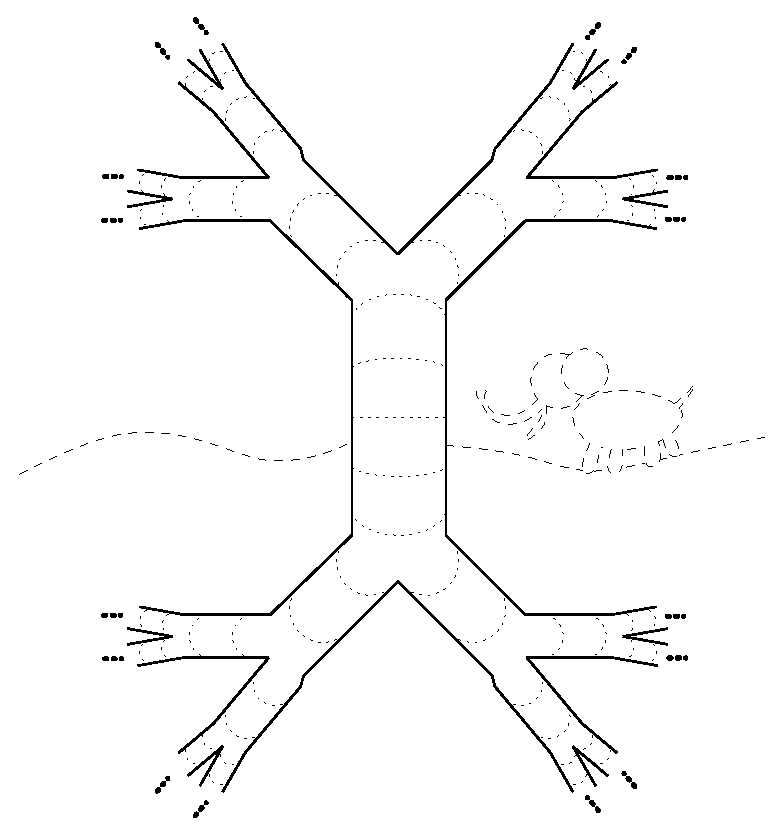
\includegraphics[width=100mm]{img/baobab.eps}
\caption{,,Baobab'', czyli oswojony do wewnątrz wielościan $X$~z~przykładu \ref{ex-o_baobabie}; rozważane w~tym przykładzie odwzorowanie $f\colon X\to X$~ma wiele wspólnego z~popularną legendą dotyczącą tego gatunku drzew.}\label{fig-baobab}
\end{figure}


%----------------------------------------------------------
%----------------------------------------------------------
%----------------------------------------------------------


\subsection{Potulność w~nieskończoności}
W~niniejszej sekcji przedstawiamy technikę dowodu twierdzenia o~punkcie lub końcu stałym, która wydaje się intuicyjna, ale ma raczej ograniczone zastosowanie. Jej istota zawiera się w~następującej obserwacji.

\begin{lem}\label{lem-ink_izo_na_hom}
Załóżmy, że $\F X$ jest \mbox{ANR-em} oraz włożenie $i\colon X\hookrightarrow \F X$ indukuje izomorfizm na grupach homologii. Wówczas homologie singularne przestrzeni $X$~są skończonego typu oraz zachodzi równość $\lambda(f)=\Ind(f)$.
\end{lem}
\begin{proof}
Ponieważ $\F X$ jest zwartym {ANR-em}, homologie tej przestrzeni są skończonego typu (patrz twierdzenie \ref{tw-westa}). Wobec tego przestrzeń $X$~również ma homologie~skończonego typu.

Niech $h_*\colon H_*(\F X)\to H_*(X)$ będzie izomorfizmem odwrotnym do izomorfizmu $H_*(i)\colon H_*(X)\to H_*(\F X)$. Zauważmy, że \begin{align*}H_*(i)\circ H_*(f)\circ h_*&=H_*(i\circ f)\circ h_*=H_*(\F f\circ i)\circ h_*\\&=H_*(\F f)\circ H_*(i)\circ h_*= H_*(\F f),\end{align*} zatem $\lambda\left(H_*(i)\circ H_*(f)\circ h_*\right)=\lambda(\F f)$. Z~drugiej strony \[\lambda(H_*(i)\circ H_*(f)\circ h_*)=\lambda(h_*\circ H_*(i)\circ H_*(f))=\lambda(H_*(f))=\lambda(f),\] co wynika z~lematu \ref{lem-1szy_lemat_o_liczbie_lefschetza}. Na podstawie~lematu \ref{lem-indeks-rowny-liczbie-lefschetza-uzwarcenia-freudenthala} ma miejsce równość $\lambda(\F f)=\Ind(f)$.\end{proof}

Istotnym przypadkiem, w~którym lemat \ref{lem-ink_izo_na_hom} ma zastosowanie, jest sytuacja, w~której $X$ jest przestrzenią potulną w nieskończoności. Jedna z~równoważnych definicji tej własności jest następująca. Mówimy, że przestrzeń $X$~będącą \mbox{ANR-em} jest \textit{potulna w nieskończoności}\footnote{ang. \textit{docile at infinity}}\index{przestrzenzzz topologiczna@przestrzeń topologiczna!potulna w nieskonzzzczonoszzzci@potulna w nieskończoności}\index{ANR!potulny w nieskonzzzczonoszzzci@potulny w nieskończoności}  \cite{Sher76}, o~ile dla każdego zwartego zbioru $A\subseteq X$ istnieje zwarty zbiór $A\subseteq B\subseteq X$ taki, że każda składowa spójności przestrzeni $X\smallsetminus B$ jest ściągalna w~$X\smallsetminus A$.

\begin{stw}\label{stw-pot_w_nsk_tw_lef}
Niech $X$ będzie potulnym w~nieskończoności \mbox{ANR-em}. Wówczas homologie singularne przestrzeni $X$~są skończonego typu oraz $\lambda(f)=\Ind(f)$.
\end{stw}
\begin{proof}
Przestrzeń $\F X$ jest \mbox{ANR-em} \cite[Theorem 4.2]{Sher76} oraz włożenie $X\hookrightarrow\F X$ jest homotopijną równoważnością \cite[Theorem 4.4]{Sher76}. Z~lematu \ref{lem-ink_izo_na_hom} otrzymujemy tezę.
\end{proof}

\begin{uw}
Stwierdzenie \ref{stw-pot_w_nsk_tw_lef} można otrzymać również jako wniosek z~twierdzenia \ref{tw-lefschetz_fpt_dla_reverse_tame}, gdyż uzwarcenie Freudenthala lokalnie zwartego, potulnego w~nieskończoności ANR-u jest $\mathcal{Z}$-uzwarceniem \cite[Theorem 4.4]{Sher76}, a~zatem taki ANR jest przestrzenią oswojoną do wewnątrz (patrz przykład \ref{przyklady-oswojonych-do-wewnatrz}).
\end{uw}

Ośrodkową, lokalnie zwartą przestrzeń metryczną $Y$ nazywamy \textit{APR-em}\footnote{ang. \textit{absolute proper retract}}\index{APR} \cite{Sher75}, jeżeli dla każdej ośrodkowej, lokalnie zwartej przestrzeni metrycznej $Z$~i~każdego włożenia $j\colon Y\hookrightarrow Z$ na podzbiór domknięty $j(Y)\subseteq Z$~takiego, że funkcja $\E(j)\colon \E(Y)\to \E(Z)$~jest różnowartościowa, istnieje właściwa retrakcja $r\colon Z\to j(Y)$.

\begin{wn}
Jeśli $X$~jest \mbox{APR-em}, to $X\in\FPEP$.
\end{wn}
\begin{proof}
Każdy \mbox{APR} jest potulnym w~nieskończoności, ściągalnym \mbox{ANR-em} \cite[Theorem 4.5]{Sher76}. Jeżeli więc $X$~jest APR-em, to dla każdego właściwego odwzorowania $g\colon X\to X$ bez końców stałych zachodzi na podstawie stwierdzenia \ref{stw-pot_w_nsk_tw_lef} równość $\lambda(g)=\Ind(g)$. Ale $\lambda(g)=1$, gdyż przestrzeń $X$~jest ściągalna. Z~własności (III) indeksu punktów stałych otrzymujemy $\Fix(g)\not=\emptyset$. 
\end{proof}

Każdy ściągalny w~sposób właściwy ANR jest APR-em \cite[Theorem 4.1]{Sher75}. Otrzymujemy stąd następujący wniosek, który odpowiada na pytanie postawione w~problemie \ref{PROBLEM-sciagalny-ma-fpep} w~przypadku, gdy rozważana przestrzeń jest ściągalna w~sposób właściwy. (Nie daje on jednak pełnej odpowiedzi na wspomniane pytanie.)

\begin{wn}\label{wn-sciagalny_w_sp_wlasciwy_to_FPEP}
Jeśli $X$ jest ściągalnym w~sposób właściwy \mbox{ANR-em}, to $X\in\FPEP$.
\end{wn}



%----------------------------------------------------------
%----------------------------------------------------------
%----------------------------------------------------------



\subsection{Końce oswojone na zewnątrz}\label{subsec-fixed_ends_dla_osw_na_zewn}
Obok obowiązujących założeń o~przestrzeni $X$~oraz odwzorowaniu $f\colon X\to X$ \textbf{do końca sekcji \ref{subsec-fixed_ends_dla_osw_na_zewn} zakładamy, że $X$~jest oswojonym na zewnątrz \mbox{ANR-em}.} Dowód twierdzenia Lefschetza o punkcie lub końcu stałym dla tego typu przestrzeni jest nieco bardziej złożony niż rozumowania przedstawione w~poprzednich sekcjach i~składa się z~kilku lematów.

\begin{lem}\label{lem-forward_tame_ma_sk_wiele_koncow}
Zbiór $\E(X)$ jest skończony.
\end{lem}
\begin{proof}
Ponieważ przestrzeń $X$~jest oswojona na zewnątrz, istnieje taki domknięty, koograniczony podzbiór $V\subseteq X$, o~dopełnieniu $C=X\smallsetminus V$, że włożenie $h_0\colon V\times\{0\}\hookrightarrow X$ rozszerza się do właściwego odwzorowania \mbox{$h\colon V\times [0,\infty)\to X$}.

Przypuśćmy, że $X$~ma nieskończenie wiele końców. Na podstawie lematu \ref{lem-malo_nieogr_skl} istnieje składowa spójności $S$~zbioru $V$~taka, że $\varepsilon(C)=S$ dla nieskończenie wielu końców $\varepsilon\in \E(X)$. Ustalmy dwa różne końce $\varepsilon_0,\varepsilon_1\in\E(X)$ o tej własności. Istnieje zbiór zwarty $D\subseteq X$ taki, że $\varepsilon_0(D)\not=\varepsilon_1(D)$. 

Ponieważ odwzorowanie $h$ jest właściwe, istnieje $t\in [0,\infty)$ o~tej własności, że $h(V,t)\cap D=\emptyset$. Funkcja $h_t=h(\cdot,t)$ jest homotopijna w~sposób właściwy odwzorowaniu $h_0$, zatem $\E(h_t)(\varepsilon_i)=\E(h_0)(\varepsilon_i)=\varepsilon_i$, gdzie $i=0,1$. Ale to oznacza, że 
\begin{equation}\label{lem-forward_tame_ma_sk_wiele_koncow-eq1} 
h_t\left(\varepsilon_i\left(h_t^{-1}(D)\right)\right)\subseteq \E(h_t)(\varepsilon_i)(D)=\varepsilon_i(D).
\end{equation}
Zachodzą inkluzje $\emptyset\not=\varepsilon_i\bigl(C\cup h_t^{-1}(D)\bigr)\subseteq \varepsilon_i(C)=S$ oraz $\varepsilon_i\bigl(C\cup h_t^{-1}(D)\bigr)\subseteq \varepsilon_i\bigl(h_t^{-1}(D)\bigr)$, zatem \begin{equation}\label{lem-forward_tame_ma_sk_wiele_koncow-eq2}\emptyset\not=\varepsilon_i\left(C\cup h_t^{-1}(D)\right)\subseteq \varepsilon_i\left(h_t^{-1}(D)\right)\cap S.\end{equation} Zestawiając~(\ref{lem-forward_tame_ma_sk_wiele_koncow-eq1})~i~(\ref{lem-forward_tame_ma_sk_wiele_koncow-eq2})~otrzymujemy $h_t(S)\cap\varepsilon_i(D)\not=\emptyset$ dla $i=0,1$. To jednak jest niemożliwe, gdyż $\varepsilon_0(D),\varepsilon_1(D)$ są różnymi składowymi spójności zbioru $X\smallsetminus D$, a~zbiór $h_t(S)$ jest spójny (jako obraz spójnego zbioru $S$) oraz $h_t(S)\cap D=\emptyset$.
\end{proof}

Dowód poniższego lematu jest wzorowany na dowodzie analogicznego wyniku dotyczącego uzwarcenia jednopunktowego, podanym w~książce Hughesa i~Ranickiego \cite{Hughes96}.  

\begin{lem}[por. {\cite[Proposition 7.11]{Hughes96}}]\label{lem-osw_nap_ANR}
Uzwarcenie Freudenthala $\F X$ przestrzeni $X$~jest \mbox{ANR-em}.
\end{lem}
\begin{proof}
Na podstawie~lematu \ref{lem-uzwarcenie_jest_metryczne} przestrzeń $\F X$ jest metryzowalna.

Wobec lematu \ref{lem-forward_tame_ma_sk_wiele_koncow} zbiór $\E(X)$ jest skończony. Oznaczmy jego elementy przez $\varepsilon_1,\ldots,\varepsilon_n$. Niech $V$ będzie domkniętym, koograniczonym podzbiorem $X$, dla którego istnieje właściwe odwzorowanie $q:V\times [0,\infty)\to X$ będące rozszerzeniem włożenia $V\times \{0\}\hookrightarrow X$; zbiór taki istnieje, gdyż przestrzeń $X$~jest oswojona na zewnątrz.

Przypuśćmy, że $\F X$ jest zanurzone jako domknięty podzbiór w~pewnej przestrzeni metrycznej $Z$. Ponieważ (będący \mbox{ANR-em}) zbiór $X=\F X\smallsetminus \E(X)$ jest domknięty w~$Z\smallsetminus \E(X)$, możemy znaleźć jego otwarte otoczenie $N$ w~$Z\smallsetminus \E(X)$ oraz retrakcję $r\colon N\to X$.

Niech $\{U_i\}_{i=1}^n$ będzie rodziną otwartych podzbiorów przestrzeni $Z$~o~następujących własnościach: $\varepsilon_i\in U_i$, $\overline{U_i}^Z\cap \overline{X\smallsetminus V}^Z=\emptyset$ oraz $\overline{U_i}^Z\cap\overline{U_j}^Z=\emptyset$ dla wszystkich $i,j=1,\ldots,n$, $i\not=j$; rodzina taka istnieje, gdyż przestrzeń $Z$~spełnia aksjomat oddzielania $\mathrm{T}_3$ (por.~\cite[Twierdzenie 1.5.5]{Engelking75}). Ustalmy zbiór $O\subseteq Z\smallsetminus \E(X)$ otwarty w~$Z\smallsetminus\E(X)$ i~taki, że \[X\subseteq O\subseteq \overline{O}^{Z\smallsetminus \E(X)}\subseteq N\] oraz \[\left(\overline{U_i}^Z\smallsetminus r^{-1}(\operatorname{Int}_X(V))\right)\cap \overline{O}^Z=\{\varepsilon_i\}\] dla wszystkich $i=1,\ldots,n$. Intuicyjnie, ,,w~pobliżu'' końców zbiór $\overline{O}^{Z\smallsetminus \E(X)}$~powinien zawierać się w~zbiorze $r^{-1}(\Int_X(V))$, otwartym w~przestrzeni $Z\smallsetminus \E(X)$.

Na podstawie~lematu Urysohna istnieje ciągła funkcja \[\rho:\left(\bigcup_{i=1}^n \overline{U_i}^Z\cup \overline{O}^Z\right)\smallsetminus \E(X)\to [0,\infty]\] taka, że $\rho^{-1}(0)=\overline{O}^Z$ oraz \[\rho^{-1}(\infty)=\left(\bigcup_{i=1}^n \overline{U_i}^Z\right)\smallsetminus \left(r^{-1}(\operatorname{Int}_X(V))\cup \E(X)\right).\] Odwzorowanie $\hat{r}:\left(\bigcup_{i=1}^{n} U_i\right)\cup O\to \F X$ określone dla $x\in\left(\bigcup_{i=1}^{n} U_i\right)\cup O$ wzorem
\[\hat{r}(x)=\begin{cases}\varepsilon_i, & \text{jeżeli } x\in \overline{U_i}^Z\smallsetminus r^{-1}(\operatorname{Int}_X(V)),\\
q(r(x),\rho(x)), & \text{jeżeli } x\in r^{-1}(V),\\
r(x), & \text{jeżeli } x\in \overline{O}^Z\smallsetminus r^{-1}(V).
\end{cases}\]
jest ciągłą retrakcją.
\end{proof}

\begin{lem}\label{lem-ANR_osw_nap_izo_hom}
Zachodzi naturalny izomorfizm $H^{\lf}_*(X)\cong H_*(\F X,\E(X))$.
\end{lem}
\begin{proof}
Zgodnie z~lematem \ref{lem-osw_nap_ANR} przestrzeń $\F X$ jest \mbox{ANR-em}. Wobec stwierdzenia \ref{stw-domkniety_podzbior_anr_jest_korozwloknieniem} włożenie skończonego zbioru dyskretnego $\E(X)$ w~przestrzeń $\F X$ jest korozwłóknieniem. Na podstawie stwierdzenia \ref{stw-homologie_ilorazu} istnieje naturalny izomorfizm \[H_*(\F X,\E(X))\cong H_*\left(\F X\big /\E(X),e\right),\] gdzie $e$~jest punktem odpowiadającym obrazowi zbioru $\E(X)$ w~przestrzeni ilorazowej $\F X\big/\E(X)$. Ale przestrzeń $\F X\big/\E(X)$ jest homeomorficzna uzwarceniu jednopunktowemu $X$ (lemat \ref{lem-iloraz_homeomorficzny_jednopunktowemu}). Zastosowanie twierdzenia \ref{tw-ranicki-hughes-izo-miedzy-homologiami-lf-a-uzwarcenia} kończy dowód.
\end{proof}

\begin{tw}\label{tw-lefschetz_fpt_dla_forward_tame}
Niech $X$~będzie oswojonym na zewnątrz \mbox{ANR-em}. Wówczas lokalnie skończone homologie $H_*^\lf(X)$ są skończonego typu i~jeśli $\lambda\left(H_*^\lf(f)\right)\not=0$, to $\Fix(f)\not=\emptyset$. Ponadto, jeżeli homomorfizm $H_*(f)$ jest dopuszczalny, to $\Lambda(f)=\lambda\left(H_*^\lf(f)\right)$.
\end{tw}
\begin{proof}
Wobec twierdzenia \ref{tw-ranicki-hughes-izo-miedzy-homologiami-lf-a-uzwarcenia} lokalnie skończone homologie $H_*^{\lf}(X)$ są izomorficzne zredukowanym homologiom singularnym zwartego \mbox{ANR-u}, a~zatem są skończenie generowane na podstawie twierdzenia \ref{tw-westa}. Liczba $\lambda\left(H_*^\lf(f)\right)$ jest więc dobrze określona. Jeżeli homomorfizm $H_*(f)$ jest dopuszczalny, to $\Lambda(f)=\lambda\left(H_*^\lf(f)\right)$ na podstawie lematu \ref{lem-rownosc_liczb_lefschetza_lf_i_zwyklej}

Wykażemy, że jeśli $\lambda\left(H_*^\lf(f)\right)\not=0$, to $\Fix(f)\not=\emptyset$. Na podstawie lematu \ref{lem-ANR_osw_nap_izo_hom} zachodzi równość: \[\lambda\left(H_*^\lf(f)\right)=\lambda\big(H_*(\F f, \E(X))\big).\] Z lematu \ref{lem-osw_nap_ANR} wiemy, że $\F X$ jest \mbox{ANR-em}. Zgodnie z~twierdzeniem \ref{tw-lefschetza_o_punkcie_stalym} odwzorowanie $\F f$ ma punkt stały w~zbiorze $\overline{\F X\smallsetminus \E(X)}=\F X$. Ale $\FixEnd(f)=\emptyset$, więc $\Fix(\F f)\cap \E(X)=\emptyset$, stąd $\F f$ ma punkt stały w~zbiorze $\F X\smallsetminus \E(X)=X$. Ponieważ $\F f\big|_X=f$, jest on również punktem stałym $f$.
\end{proof}

W~przypadku oswojonych na zewnątrz ANR-ów nie jest znana odpowiedź na pytanie o~związek liczby Lefschetza z~indeksem punktów stałych, postawione w~problemie \ref{PROBLEM-twierdzenie-o-indeksie}.

Poniżej podajemy przykład oswojonego na zewnątrz, lokalnie zwartego wielościanu $X$~oraz właściwego odwzorowania bez końców stałych $f\colon X\to X$ o~tej własności, że liczba $\lambda\left(H_*^\lf(f)\right)$ jest dobrze określona, ale homomorfizmy $H_*(f)$, $H_*^\infty(f)$ nie są dopuszczalne.

\begin{ex}\label{ex-osw_do_wew_bez_l_lef}
Dla każdej liczby naturalnej $n$~niech \[A_n=\left\{(x,y)\in\mathbb{R}^2:x^2+(y-2n)^2=1\right\}.\] Za przestrzeń $X$~przyjmijmy (przedstawiony na rysunku \ref{fig-organy}) zbiór
\[X=\bigcup_{n\in\mN}A_n\times \bigl( (-\infty,-n]\cup [n,\infty) \bigr),\] 
z~topologią indukowaną z~$\mathbb{R}^3$, zaś $f\colon X\to X$ niech będzie dla $(x,y,z)\in X$ dane wzorem $f(x,y,z)=(x,y,-z)$. Oczywiście odwzorowanie $f$~jest właściwe i~$\FixEnd(f)=\emptyset$. Nietrudno również spostrzec, że $X$~jest oswojonym na zewnątrz wielościanem, wobec czego liczba $\lambda^{\lf}(f)$ jest dobrze określona na podstawie twierdzenia \ref{tw-lefschetz_fpt_dla_forward_tame}. Jednak homomorfizmy $H_*(f)$, $H^\infty_*(f)$ nie są, jak łatwo zauważyć, dopuszczalne.
\end{ex}

\begin{figure}[h]
\centering
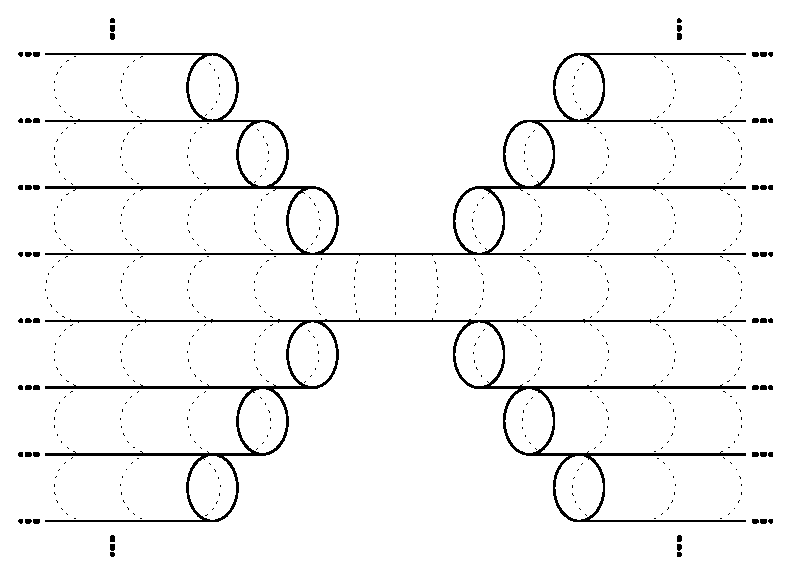
\includegraphics[width=100mm]{img/organki.eps}
\caption{,,Piszczałki organowe'', czyli oswojony na zewnątrz wielościan $X$~z~przykładu \ref{ex-osw_do_wew_bez_l_lef}.}\label{fig-organy}
\end{figure}




%----------------------------------------------------------
%----------------------------------------------------------
%----------------------------------------------------------




\section{Kombinatoryczne twierdzenia o~punkcie lub końcu stałym}\label{sec-komb_twi_o_punkcie_stalym}

W~niniejszym podrozdziale przenosimy podstawowe definicje związane z~końcami stałymi z~przypadku ciągłego na teorioporządkowy oraz symplicjalny, a~także rozwiązujemy dyskretne odpowiedniki problemów \ref{PROBLEM-twierdzenie-lefschetza-o-punkcie-lub-koncu-stalym}, \ref{PROBLEM-twierdzenie-o-indeksie}, \ref{PROBLEM-sciagalny-ma-fpep}. Otrzymujemy twierdzenia typu Lefschetza o~punkcie lub końcu stałym dla odwzorowań zachowujących porządek oraz odwzorowań symplicjalnych. Badamy ponadto związki własności punktu lub końca stałego z~pojęciem (ko)rozbieralności oraz z~operacją iloczynu kartezjańskiego zbiorów częściowo uporządkowanych.

\subsection{Definicje}
Zachowujące porządek odwzorowanie  $f\colon P\to Q$ nazywamy \textit{właściwym}\index{odwzorowanie!zachowujazzzce porzazzzdek@zachowujące porządek!wlzzzaszzzciwe@właściwe}, jeśli dla każdego $q\in Q$ zbiór $f^{-1}(q)$ jest skończony.

\textit{Końcem}\index{koniec!czezzzszzzciowego porzazzzdku@częściowego porządku} lokalnie skończonego częściowego porządku $P$~nazywamy funkcję \[\varepsilon\colon \{A\subseteq P:A\text{ jest skończony}\}\to 2^P\] spełniającą następujące warunki:
\begin{compactitem}
\item[---] jeżeli $A\subseteq B$ są skończonymi zbiorami zawartymi w~$P$, to $\varepsilon(B)\subseteq \varepsilon(A)$;
\item[---] dla każdego skończonego zbioru $A\subseteq P$ zbiór $\varepsilon(A)$ jest nieskończoną składową spójności częściowego porządku $P\smallsetminus A$.
\end{compactitem}
Zbiór końców porządku $P$~oznaczamy symbolem $\E(P)$.\nomenclature[6aa]{$\E$}{zb. koncow porzadku XXX do zbioru koncow zwyklego dopisz drugi numer strony}\index{zbiozzzr@zbiór!konzzzcozzzw@końców!czezzzszzzciowego porzazzzdku@częściowego porządku}

Jeśli $f\colon P\to Q$ jest właściwym odwzorowaniem zachowującym porządek między lokalnie skończonymi częściowymi porządkami, to możemy zadać odwzorowanie $\E(f)\colon \E(P)\to \E(Q)$ w~następujący sposób. Dla $\varepsilon\in \E(P)$ i~skończonego zbioru $A\subseteq Q$ niech $\E(f)(\varepsilon)(A)$ będzie jedyną spójną składową zbioru $Q\smallsetminus A$ taką, że \[f\left(\varepsilon\left(f^{-1}(A)\right)\right)\subseteq \E(f)(\varepsilon)(A).\] Przyporządkowanie $\E$ jest funktorialne.

Analogicznie jak w~przypadku ciągłych odwzorowań definiujemy \textit{koniec stały}\index{koniec!stalzzzy odwzorowania@stały odwzorowania!zachowujazzzcego porzazzzdek@zachowującego porządek} właściwego, zachowującego porządek odwzorowania $f\colon P\to P$ lokalnie skończonego częściowego porządku $P$~w~siebie, zbiór końców stałych $\FixEnd(f)$\nomenclature[3ba]{$\FixEnd(f)$}{wersja porzadkowa XXX}\index{zbiozzzr@zbiór!konzzzcozzzw stalzzzych odwzorowania@końców stałych odwzorowania!zachowujazzzcego porzazzzdek@zachowującego porządek} takiego odwzorowania oraz \textit{własność punktu lub końca stałego}\index{wlzzzasnoszzzczzz@własność!punktu lub konzzzca stalzzzego@punktu lub końca stałego!czezzzsciowego porzazzzdku@częściowego porządku}\index{czezzzszzzciowy porzazzzdek@częściowy porządek!ma wlzzzasnoszzzc@ma własność!punktu lub konzzzca stalzzzego@punktu lub końca stałego} ($\FPEP$)\nomenclature[3la]{$\FPEP$}{teorioporzadkowy XXX} ze względu na właściwe, zachowujące porządek przekształcenia. Dla lokalnie skończonego częściowego porządku $P$~i~właściwego odwzorowania $f\colon P\to P$ bez końców stałych definiujemy \textit{zbiór przestawiający końce}\index{zbiozzzr@zbiór!przestawiajazzzcy konzzzce@przestawiający końce!w czezzzsciowym porzazzzdku@w częściowym porządku} jako taki skończony zbiór $D\subseteq P$, że $f(\varepsilon(D))\cap \varepsilon(D)=\emptyset$ dla każdego końca $\varepsilon\in\E(X)$. Jeżeli porządek $P$~jest spójny, to zbiór taki istnieje, a~ponadto założyć o~nim można, że $P\smallsetminus D$ ma jedynie nieskończone składowe spójności. Faktów tych dowodzimy podobnie jak w~przypadku ciągłym.

Przez \textit{koniec}\index{koniec!kompleksu symplicjalnego} lokalnie skończonego kompleksu symplicjalnego $K$~rozumiemy koniec częściowego porządku $\mP(K)$; piszemy $\E(K)=\E(\mP(K))$\index{zbiozzzr@zbiór!konzzzcozzzw@końców!kompleksu symplicjalnego}. Odwzorowanie symplicjalne $\varphi\colon K\to L$ nazywamy \textit{właściwym}\index{odwzorowanie!symplicjalne!wlzzzaszzzciwe@właściwe}, o~ile funkcja zachowująca porządek $\mP(\varphi)\colon \mP(K)\to\mP(L)$ jest właściwa, lub równoważnie, o~ile realizacja geometryczna $|\varphi|\colon |K|\to |L|$ jest właściwym odwzorowaniem. Przyjmujemy oznaczenie $\E(\varphi)=\E(\mP(\varphi))$. Nietrudno jest wskazać naturalną bijekcję $\xi_K\colon \E(\mP(K))\to \E(|K|)$.

Jeśli $K$~jest lokalnie skończonym kompleksem symplicjalnym, to mówimy, że $K$~ma \textit{własność sympleksu lub końca stałego}\index{wlzzzasnoszzzczzz@własność!sympleksu lub konzzzca stalzzzego@sympleksu lub końca stałego}\index{kompleks symplicjalny!ma wlzzzasnoszzzc@ma własność!sympleksu lub konzzzca stalzzzego@sympleksu lub końca stałego} i~piszemy $K\in\FSEP$\nomenclature[3j]{$K\in\FSEP$}{lokalnie skończony kompleks symplicjalny $K$~ma własność sympleksu lub końca stałego}, o~ile dla każdego właściwego odwzorowania symplicjalnego $\varphi\colon K\to K$ istnieje sympleks stały lub \textit{koniec stały}\index{koniec!stalzzzy odwzorowania@stały odwzorowania!symplicjalnego}, tj.~taki koniec $\varepsilon\in \E(K)$, że $\E(\varphi)(\varepsilon)=\varepsilon$.

Oczywiście istnienie sympleksu stałego odwzorowania symplicjalnego implikuje istnienie punktu stałego jego realizacji geometrycznej, zaś każdy koniec stały odwzorowania symplicjalnego można utożsamiać (poprzez bijekcję $\xi_K$) z~końcem stałym realizacji geometrycznej tego odwzorowania.

Własność sympleksu lub końca stałego jest równoważna własności punktu lub końca stałego stowarzyszonego częściowego porządku.

\begin{stw}[por.~{\cite[Proposition 6.3.15]{Schroder03}}]\label{stw-simplicial_fpep_wtw_order_theoretic}
Jeżeli $K$~jest lokalnie skończonym kompleksem symplicjalnym, to $K\in\FSEP$ wtedy i~tylko wtedy, gdy $\mP(K)\in\FPEP$.
\end{stw}
\begin{proof}
Ustalmy lokalnie skończony kompleks symplicjalny $K$. 

Załóżmy, że $\mP(K)\in\FPEP$; niech $\varphi\colon K\to K$ będzie właściwym odwzorowaniem symplicjalnym bez końców stałych. Wówczas $\FixEnd(\mP(\varphi))=\emptyset$, więc $\Fix(\mP(\varphi))\not=\emptyset$, co oznacza, że istnieje sympleks $\sigma$~kompleksu $K$~taki, że $\varphi(\sigma)=\sigma$. Wobec tego $K\in\FSEP$.

Załóżmy teraz, że $K\in\FSEP$ i~ustalmy właściwe, zachowujące porządek odwzorowanie $f\colon \mP(K)\to \mP(K)$ bez końców stałych. Dla każdego wierzchołka $v$~kompleksu $K$~wybierzmy dowolny element $g_v\in f(\{v\})$. Określmy funkcję $g\colon \mP(K)\to \mP(K)$, dla $\sigma\in \mP(K)$ przyjmując $g(\sigma)=\bigcup_{v\in\sigma}\{g_v\}$. Oczywiście $g$~zachowuje porządek. Nietrudno również sprawdzić (por.~\cite[Lemma 6.3.14]{Schroder03}), że odwzorowanie $\gamma\colon K\to K$ zadane na wierzchołkach $v\in K$ wzorem $\gamma(v)=g_v$ jest symplicjalne oraz $\mP(\gamma)=g$. Dla każdego sympleksu $\sigma\in \mP(K)$ i~każdego wierzchołka $v\in\sigma$ mamy $f(\sigma)\supseteq f(\{v\})\supseteq \{g_v\}= g(\{v\})$, więc $f(\sigma)\supseteq\bigcup_{v\in \sigma} g(\{v\})=g(\sigma)$. Jak łatwo zauważyć, wynika stąd, że $\E(g)=\E(f)$, czyli w~szczególności $\FixEnd(g)=\FixEnd(f)=\emptyset$. Ponieważ $g=\mP(\gamma)$, odwzorowanie $\gamma$~nie ma końców stałych, a~zatem istnieje sympleks stały $\sigma$~tego odwzorowania. Ale $f(\sigma)\supseteq g(\sigma)=\sigma$, więc na podstawie twierdzenia Abiana-Browna \ref{tw-abiana_browna} funkcja $f$~ma punkt stały, co kończy dowód stwierdzenia.
\end{proof}



%--------------------------------------------------------------------
%--------------------------------------------------------------------
%--------------------------------------------------------------------



\subsection{Odległość w~częściowym porządku}
Bieżąca sekcja poświęcona jest pomocniczemu pojęciu odległości między elementami częściowego porządku, które wykorzystane zostanie w~dalszej części rozdziału.

Jeżeli $p,q$ są elementami częściowego porządku $P$, to przez $d_P(p,q)$\nomenclature[4k]{$d_P(p,q)$}{odległość między elementami $p, q$~częściowego porządku $P$} oznaczamy \textit{odległość}\index{odleglzzzoszzzczzz w czezzzszzzciowym porzazzzdku@odległość w~częściowym porządku} $p$~od~$q$~w~zbiorze $P$, z~definicji równą minimalnej długości ścieżki prowadzącej z~$p$~do $q$~w~grafie porównywalności $\Comp(P)$, o~ile ścieżka taka istnieje; w~przeciwnym wypadku przyjmujemy $d_P(p,q)=\infty$. Dla $p\in P$ oraz $A\subseteq P$ niech $d_P(p,A)=\min\{d_P(p,q):q\in A\}$.\nomenclature[4l]{$d_P(p,A)$}{odległość punktu $p$~od zbioru $A$~w~częściowym porządku $P$}

Jeśli $f\colon P\to Q$ jest zachowującym porządek odwzorowaniem, to dla każdej ścieżki $(p_0,\ldots,p_n)$ w~$\Comp(P)$ ciąg $\big(f(p_0),\ldots,f(p_n)\big)$ jest ścieżką w~$\Comp(Q)$, zatem $d_Q(f(p),f(q))\leq d_P(p,q)$ dla wszystkich $p,q\in P$.

Dla częściowego porządku $P$, elementu $p\in P$ oraz liczby $n\in \mN$ przyjmujemy oznaczenie \[B_P(p,n)=\{q\in P:d_P(p,q)\leq n\}.\]\nomenclature[4m]{$B_P(p,n)$}{domknięta kula o~środku $p$~i~promieniu~$n$~w~zbiorze częściowo uporządkowanym $P$} Ponadto, jeśli $F\subseteq P$, to definiujemy zbiór \[B_P(F,n)=\bigcup_{p\in F}B_P(p,n)=\{q\in P:d_P(q,F)\leq n\}.\]\nomenclature[4n]{$B_P(A,n)$}{domknięta otoczka zbioru $A$~o~promieniu~$n$~w~zbiorze częściowo uporządkowanym $P$}Nietrudno spostrzec, że jeśli porządek $P$~jest lokalnie skończony, to dla każdego skończonego podzbioru $F\subseteq P$ oraz każdego $n\in\mN$~zbiór $B_P(F,n)$ jest skończony.

\begin{lem}\label{lem-odleglosc_miedzy_skladowymi_po_nadmuchaniu_srodka}
Niech $P$~będzie spójnym częściowym porządkiem, $F\subseteq P$ jego skończonym podzbiorem, $S\subseteq P$ składową spójności zbioru $P\smallsetminus F$ oraz niech $k\in\mN$. Wówczas $d_P(p,q)> k$ dla wszystkich $p\in S$, $q\in P\smallsetminus \left(S\cup B_P(F,k)\right)$.
\end{lem}
\begin{proof}
Zauważmy, że dla wszystkich elementów $p\in S$ oraz $q\in P\smallsetminus (S\cup F)$ każda ścieżka prosta w~grafie porównywalności $\Comp(P)$ prowadząca z~$p$~do $q$~zawiera element zbioru $F$; zachodzi zatem nierówność \[d_P(p,q)\geq d_P(p,F)+d_P(q,F).\] Wobec tego dla $p\in S$ oraz $q\in P\smallsetminus \left(S\cup B_P(F,k)\right)$ mamy \[d_P(p,q)\geq d_P(p,F)+d_P(q,F)\geq d_P(p,F)+k+1>k.\qedhere\] 
\end{proof}

\begin{lem}\label{lem-bliskie_funkcje_to_samo_na_koncach}
Niech $P,Q$~będą lokalnie skończonymi częściowymi porządkami, zaś $f,g\colon P\to Q$ właściwymi odwzorowaniami zachowującymi porządek. Jeżeli istnieje $k\in\mN$ takie, że dla każdego $p\in P$ zachodzi nierówność $d_Q(f(p),g(p))\leq k$, to $\E(f)=\E(g)$.
\end{lem}
\begin{proof}
Załóżmy, że istnieje liczba $k\in \mN$ taka, że $d_Q(f(p),g(p))\leq k$ dla każdego $p\in P$. Aby udowodnić równość $\E(f)=\E(g)$ wystarczy wykazać, że dla każdego końca $\varepsilon\in \E(P)$ i~każdego skończonego podzbioru $F\subseteq Q$ mamy 
\mbox{$\E(f)(\varepsilon)(F)\cap \E(g)(\varepsilon)(F)\not=\emptyset$}. Ustalmy zatem koniec $\varepsilon\in \E(P)$ oraz skończony zbiór $F\subseteq Q$. 

Zauważmy, że \[g^{-1}(F)\subseteq f^{-1}\big(B_Q(F,k)\big)\supseteq f^{-1}(F),\] więc \[\varepsilon\big(g^{-1}(F)\big)\supseteq \varepsilon\left(f^{-1}\big(B_Q(F,k)\big)\right)\subseteq \varepsilon\big(f^{-1}(F)\big).\]
Ustalmy $p\in \varepsilon\bigl(f^{-1}\big(B_Q(F,k)\big)\bigr)$; mamy \begin{align*}f(p)&\in f\left( \varepsilon\big(f^{-1}(F)\big)\right)\subseteq \E(f)(\varepsilon)(F),\\ g(p)&\in  g\left(\varepsilon\big(g^{-1}(F)\big)\right)\subseteq \E(g)(\varepsilon)(F)\end{align*} oraz $d_Q(f(p),F)>k$. Ale $d_Q(f(p),g(p))<k$, więc $g(p)\in \E(f)(\varepsilon)(F)$ na podstawie lematu \ref{lem-odleglosc_miedzy_skladowymi_po_nadmuchaniu_srodka}. Wobec tego $\E(f)(\varepsilon)(F)\cap \E(g)(\varepsilon)(F)\not=\emptyset$.
\end{proof}


%-------------------------------------------------------------------
%-------------------------------------------------------------------
%-------------------------------------------------------------------




\subsection{Kombinatoryczne twierdzenie typu Lefschetza o~punkcie lub końcu stałym}\label{subsec-komb_twi_lefschetza}
\textbf{Odtąd, aż do końca sekcji \ref{subsec-komb_twi_lefschetza}, zakładamy, że $P$~jest spójnym, lokalnie skończonym częściowym porządkiem, zaś $f\colon P\to P$ jest właściwym odwzorowaniem zachowującym porządek bez końców stałych.}

Jeśli $h\colon A\to A$ jest funkcją określoną na pewnym zbiorze $A$, to mówimy, że $a\in A$ jest jej \textit{punktem periodycznym}\index{punkt!periodyczny}, o ile $h^m(a)=a$ dla pewnej liczby naturalnej $m\geq 1$. Jeżeli natomiast istnieje liczba naturalna $n$ taka, że $h^{n}(a)$ jest punktem periodycznym funkcji $h$, to $a$ nazywamy \textit{punktem ostatecznie periodycznym}\index{punkt!ostatecznie periodyczny} funkcji $h$.

\begin{lem}\label{lem-kazdy_punkt_ost_periodyczny}
Każdy element $p\in P$ jest punktem ostatecznie periodycznym odwzorowania~$f$. 
\end{lem}
\begin{proof}
Ustalmy element $p\in P$ i~przypuśćmy, że nie jest on punktem ostatecznie periodycznym funkcji $f$. Przyjmijmy oznaczenie $k=d_P(p,f(p))$; porządek $P$~jest spójny, więc $k<\infty$. Ponieważ $f$~zachowuje porządek, prawdziwa jest dla wszystkich $n\in\mN$ nierówność 
\begin{equation}d_P\left(f^n(p),f^{n+1}(p)\right)\leq k.\label{eq_lem-kazdy_punkt_1}\end{equation} Istnieje podzbiór $D\subseteq P$ przestawiający końce i~taki, że $P\smallsetminus D$ nie ma skończonych składowych spójności.  Ponieważ punkt $p$~nie jest ostatecznie periodyczny, a~zbiór $B_P(D,k)$~jest skończony, istnieje liczba $n_0\in\mN$ taka, że $f^n(p)\not\in B_P(D,k)$ dla wszystkich $n\geq n_0$. W~szczególności $f^{n_0}(p)\not\in D$, więc $f^{n_0}(p)\in \varepsilon(D)$ dla pewnego końca $\varepsilon\in\E(P)$. Ponieważ $D$~jest zbiorem przestawiającym końce, $f^{n_0+1}(p)\not\in \varepsilon(D)$, a~z~wyboru liczby $n_0$~element $f^{n_0+1}(p)\not\in B_P(D,k)$. Zatem $f^{n_0+1}(p)\in P\smallsetminus (\varepsilon(D)\cup B_P(D,k))$. Na podstawie lematu \ref{lem-odleglosc_miedzy_skladowymi_po_nadmuchaniu_srodka} zachodzi nierówność $d_P\left(f^{n_0+1}(p),f^{n_0}(p)\right)> k$, sprzeczna z~nierównością (\ref{eq_lem-kazdy_punkt_1}).
\end{proof}

\begin{lem}\label{lem-wsz_per_odw_aut}
Niech $Q$~będzie częściowym porządkiem, zaś $g\colon Q\to Q$ zachowującym porządek odwzorowaniem o~tej własności, że każdy element zbioru $Q$ jest punktem periodycznym funkcji~$g$. Wówczas $g$~jest automorfizmem częściowego porządku $Q$.
\end{lem}
\begin{proof}
Dowód lematu jest nietrudny; należy zauważyć, że odwzorowanie $g$~jest różnowartościowe i~,,na'', oraz że jeśli $g(p)\leq g(q)$ dla pewnych $p,q\in Q$, to również $p\leq q$. Dla przykładu udowodnimy tę ostatnią własność. 

Jeśli $p\leq q$, to $g^n(p)\leq g^n(q)$ dla każdej liczby $n\in\mN$. Ponieważ $p,q$ są punktami periodycznymi funkcji $g$, istnieją liczby naturalne $n_p,n_q$ takie, że $g^{n_p}(p)=p$ oraz $g^{n_q}(q)=q$, a~zatem: \[p=g^{n_p n_q}(p)\leq g^{n_p n_q}(q)=q.\qedhere\]
\end{proof}

Oznaczmy przez $P_\infty$~podzbiór częściowo uporządkowany zbioru $P$, którego elementami są wszystkie punkty periodyczne odwzorowania $f$. Oczywiście $f(P_\infty)\subseteq P_\infty$. Niech $f_\infty=f\big |_{P_\infty}\colon P_\infty\to P_\infty$. Na podstawie lematu \ref{lem-wsz_per_odw_aut} odwzorowanie to jest automorfizmem częściowego porządku $P_\infty$. Ponieważ \mbox{$\FixEnd(f)=\emptyset$}, jest oczywiste, że $\FixEnd(f_\infty)=\emptyset$.

Przypomnijmy, że z~definicji homologie częściowego porządku $Q$~są równe symplicjalnym homologiom stowarzyszonego z~nim kompleksu symplicjalnego $\mK(Q)$. Są to zatem homologie pewnego kompleksu łańcuchowego $C_*(Q)=\left(C_i(Q),\partial_i\right)_{i\in\mN}$ takiego, że dla każdego $i\in\mN$ bazą przestrzeni wektorowej $C_i(Q)$~jest zbiór łańcuchów długości $i$~zawartych w~$Q$. Jeżeli $A\subseteq Q$, to istnieje kompleks łańcuchowy $C_*(Q,A)=C_*(Q)\big/C_*(A)$ oraz $H_*(Q,A)=H_*(C_*(Q,A))$.

Jeżeli $Q$~jest częściowym porządkiem, $A\subseteq Q$, zaś $g\colon Q\to Q$ jest zachowującym porządek odwzorowaniem o~tej własności, że $g(A)\subseteq A$, to symbolem $g_{(Q,A)}\colon (Q,A)\to (Q,A)$ oznaczamy indukowane przez $g$~odwzorowanie par częściowych porządków.

\begin{lem}\label{lem-lambda_phi_nsk_rowna_lambda_phi}
Homomorfizm $H_*(f)$~jest dopuszczalny wtedy i~tylko wtedy, gdy homomorfizm $H_*(f_\infty)$ jest dopuszczalny. Ponadto zachodzi wówczas równość uogólnionych liczb Lefschetza: $\Lambda(f)=\Lambda(f_\infty)$.
\end{lem}
\begin{proof}
Istnieje przemienny diagram \[\xymatrix{\cdots \ar[r] & H_n(P_\infty)\ar[r]\ar^{H_n(f_\infty)}[d] & H_n(P)\ar^{H_n(f)}[d]\ar[r] & H_n(P,P_\infty)\ar[r]\ar^{H_n\left(f_{(P,P_\infty)}\right)}[d] & H_{n-1}(P_\infty)\ar[r]\ar^{H_{n-1}(f_\infty)}[d] & \cdots\\ \cdots\ar[r] & H_n(P_\infty)\ar[r] & H_n(P)\ar[r] & H_n(P,P_\infty)\ar[r] & H_{n-1}(P_\infty)\ar[r] & \cdots}\] o wierszach będących długimi ciągami dokładnymi pary $(P,P_\infty)$. Dla każdego elementu $\zeta\in H_*(P,P_\infty)$ istnieje łańcuch $z\in C_*(P)$ taki, że $\zeta$~jest klasą homologii elementu $z+C_*(P_\infty)\in C_*(P)\big/C_*(P_\infty)$, co zapisujemy przez $\zeta=[z+C_*(P_\infty)]$. Na podstawie lematu \ref{lem-kazdy_punkt_ost_periodyczny} istnieje liczba naturalna $n_z$~taka, że $C_*(f^{n_z})(z)\in C_*(P_\infty)$. Zatem \[H_*\left(f^{n_z}_{(P,P_\infty)}\right)(\zeta)=H_*\left(f^{n_z}_{(P,P_\infty)}\right)([z+C_*(P_\infty)])=[C_*(f^{n_z})(z)+C_*(P_\infty)]=0,\] czyli $\zeta$~należy do uogólnionego jądra: $\zeta\in N\bigl(H_*\bigl(f_{(P,P_\infty)}\bigr)\bigr)$. Wobec~dowolności wyboru $\zeta\in H_*(P,P_\infty)$~oznacza to, że homomorfizm $H_*\bigl(f_{(P,P_\infty)}\bigr)$ jest dopuszczalny oraz $\Lambda\bigl(H_*\bigl(f_{(P,P_\infty)}\bigr)\bigr)=0$. Z~lematu \ref{lem-2gi_lemat_o_liczbie_lefschetza} otrzymujemy równość $\Lambda(f)=\Lambda(f_\infty)$.
\end{proof}

Poniższe twierdzenie typu Lefschetza o~punkcie lub końcu stałym dla częściowych porządków jest uogólnieniem na lokalnie skończone częściowe porządki twierdzenia \ref{tw-baclawski-bjorner}.

\begin{tw}\label{tw-order-theoretic-fixed-point-or-end-theorem}
Jeśli homomorfizm $H_*(f)$ jest dopuszczalny, to zachodzi równość uogólnionej liczby Lefschetza odwzorowania $f$~oraz charakterystyki Eulera zbioru jego punktów stałych: $\Lambda(f)=\chi(\Fix(f))$.
\end{tw}
\begin{proof}
Załóżmy, że homomorfizm $H_*(f)$~jest dopuszczalny. Wybierzmy skończony podzbiór $D'\subseteq P_\infty$ taki, że $D'$~jest dla $f_\infty$ zbiorem przestawiającym końce. Ponieważ $f_\infty$ jest automorfizmem, możemy zakładać, że podzbiór $D'$ jest niezmienniczy ze względu na działanie $f_\infty$. Co więcej, możemy $D'$~rozszerzyć do niezmienniczego ze względu na $f_\infty$, skończonego podzbioru $D\subseteq P$ takiego, że zbiór $P_\infty\smallsetminus D$ nie ma skończonych składowych spójności.

Niech $A=P_\infty\smallsetminus D$. Wobec wyboru $D$ zbiór $A$ jest niezmienniczy ze względu na działanie automorfizmu $f_\infty$. Ponieważ zbiór $D=P_\infty\smallsetminus A$ jest skończony, kompleks łańcuchowy $C_*(P_\infty,A)$ oraz relatywne homologie $H_*(P_\infty,A)$ są skończonego typu. Istnieje przemienny diagram
\[
\xymatrix@R=30pt{\cdots\ar[r]& H_n(A)\ar[r]\ar[d]^{H_n\bigl(f\big |_A\bigr)}& H_n(P_\infty)\ar[r]\ar[d]^{H_n(f_\infty)} & H_n(P_\infty,A)\ar[r]\ar[d]^{H_n\bigl({f_\infty}_{(P_\infty,A)}\bigr)} & H_{n-1}(A)\ar[r]\ar[d]^{H_{n-1}\bigl(f\big |_A\bigr)} & \cdots\\
\cdots\ar[r]& H_n(A)\ar[r]& H_n(P_\infty)\ar[r] & H_n(P_\infty,A)\ar[r] & H_{n-1}(A)\ar[r] & \cdots}
\]
o~wierszach będących długimi ciągami dokładnymi pary $(P_\infty,A)$.
Homomorfizmy $H_*\bigl({f_\infty}_{(P_\infty,A)}\bigr)$ oraz $H_*(f_\infty)$ są dopuszczalne, co wynika odpowiednio z~faktu, że homologie $H_*(P_\infty,A)$ są skończonego typu i~z~lematu \ref{lem-lambda_phi_nsk_rowna_lambda_phi}. Na podstawie lematu \ref{lem-2gi_lemat_o_liczbie_lefschetza} homomorfizm $H_*\bigl(f\big |_A\bigr)$ jest dopuszczalny oraz \[\Lambda\bigl(f\big |_A\bigr)=\Lambda(f_\infty)-\Lambda\bigl({f_\infty}_{(P_\infty,A)}\bigr).\]

Niech $S_i$, $i=1,\ldots,k$, będą wszystkimi spójnymi składowymi zbioru $A$. Ponieważ $D$~jest dla $f_\infty$~zbiorem przestawiającym końce, dla wszystkich $i=1,\ldots,k$ mamy $f_\infty(S_i)\cap S_i=\emptyset$. Wobec teorioporządkowego odpowiednika lematu \ref{lem-permutowanie-skladowych-a-liczba-lefschetza} oznacza to, że $\Lambda\bigl(f\big |_A\bigr)=0$, czyli $\Lambda(f_\infty)=\Lambda\bigl({f_\infty}_{(P,A)}\bigr)$. Z~lematu \ref{lem-lambda_phi_nsk_rowna_lambda_phi} otrzymujemy równość $\Lambda(f)=\Lambda\bigl({f_\infty}_{(P,A)}\bigr)$.

Kompleks łańcuchowy $C_*(P_\infty,A)$ jest skończonego typu, wobec czego na podstawie~twierdzenia \ref{tw-lefschetza-hopfa} zachodzą równości \[\lambda\left(C_*\bigl({f_\infty}_{(P,A)}\bigr)\right)=\lambda\left(H_*\bigl({f_\infty}_{(P,A)}\bigr)\right)=\Lambda\bigl({f_\infty}_{(P,A)}\bigr).\] Bazę przestrzeni $C_*(P_\infty,A)$ tworzą skończone, liniowo uporządkowane podzbiory $P_\infty$~nie zawierające się w~$A$. Dla takiego bazowego podzbioru liniowo uporządkowanego $l\subseteq P_\infty$ oraz~skalara $\alpha\in\mathbb{Q}\smallsetminus \{0\}$ równość $C_*\bigl({f_\infty}_{(P,A)}\bigr)(l)=\alpha l$ ma miejsce wtedy i~tylko wtedy, gdy $f_\infty(l)=l$ oraz $\alpha=1$, gdyż $f_\infty$~jest odwzorowaniem zachowującym porządek. Ponieważ $\Fix(f_\infty)\subseteq P_\infty\smallsetminus A$, każdy bazowy podzbiór liniowo uporządkowany $l\subseteq P_\infty$~taki, że $C_*\bigl({f_\infty}_{(P,A)}\bigr)(l)=l$, jest również elementem bazowym przestrzeni liniowej $C_*(D)\subseteq C_*(P_\infty,A)$. Zachodzą  zatem równości \begin{align*}\lambda(C_*(f_\infty,A))&=\lambda\left(C_*\bigl(f\big |_D\bigr)\right)=\sum_{i=0}^{\infty}(-1)^i\tr\left(C_i\bigl(f\big|_D\bigr)\right)\\&=\sum_{i=0}^{\infty}(-1)^{i}\moc{\bigl\{\{q_0<\ldots<q_i\}\subseteq \Fix(f)\bigr\}} =\chi(\Fix(f)),\end{align*}
kończące dowód twierdzenia. 
\end{proof}

Oczywisty jest następujący wniosek.
\begin{wn}
Jeśli homomorfizm $H_*(f)$~jest dopuszczalny oraz~$\Lambda(f)\not=0$, to $\Fix(f)\not=\emptyset$.
\end{wn}

Prawdziwa jest także symplicjalna wersja twierdzenia \ref{tw-order-theoretic-fixed-point-or-end-theorem}, uogólniająca wniosek \ref{wn-baclawski-bjorner}.

\begin{wn}\label{wn-simplicial-fixed-point-or-end-theorem}
Niech $K$~będzie lokalnie skończonym kompleksem symplicjalnym, zaś $\varphi\colon K\to K$ właściwym odwzorowaniem symplicjalnym bez końców stałych. Jeśli homomorfizm $H_*(\varphi)$ jest dopuszczalny, to jego uogólniona liczba Lefschetza jest równa charakterystyce Eulera zbioru punktów stałych realizacji geometrycznej tego odwzorowania: $\Lambda(\varphi)=\chi(\Fix|\varphi|)$. 
\end{wn}
\begin{proof}
Oczywiście $\mP(\mK(\mP(K)))$ jest lokalnie skończonym częściowym porządkiem, zaś $\mP(\mK(\mP(\varphi)))$ jest właściwym odwzorowaniem zachowującym porządek bez końców stałych. Ponadto, jeśli homomorfizm $H_*(\varphi)$ jest dopuszczalny, to również homomorfizm $H_*(\mP(\mK(\mP(\varphi))))$ jest dopuszczalny i~zachodzi równość $\Lambda(\varphi)=\Lambda(\mP(\mK(\mP(\varphi))))$. Z~twierdzenia \ref{tw-order-theoretic-fixed-point-or-end-theorem} otrzymujemy: \[\Lambda(\varphi)=\chi(\Fix(\mP(\mK(\mP(\varphi)))))=\chi(\Fix(|\mK(\mP(\varphi))|))=\chi(\Fix(|\varphi|)).\qedhere\]
\end{proof}

Zauważmy, że funkcja z~przykładu \ref{ex-jacob-ladder} jest realizacją geometryczną odwzorowania symplicjalnego, co pokazuje, że w~powyższych wynikach nie można pominąć założenia o~dopuszczalności homomorfizmów indukowanych przez rozważane odwzorowania.

Poniższe twierdzenie wiąże uogólnioną liczbę Lefschetza odwzorowania symplicjalnego bez końców stałych z~indeksem punktów stałych jego realizacji geometrycznej.

\begin{tw}\label{tw-rownosc_indeksu_i_l_lefschetza_odwz_sympl}
Niech $K$~będzie lokalnie skończonym kompleksem symplicjalnym, zaś $\varphi\colon K\to K$ właściwym odwzorowaniem symplicjalnym bez końców stałych. Jeśli homomorfizm $H_*(\varphi)$ jest dopuszczalny, to uogólniona liczba Lefschetza odwzorowania symplicjalnego $\varphi$~jest równa indeksowi punktów stałych jego realizacji geometrycznej: $\Lambda(\varphi)=\Ind(|\varphi|)$.
\end{tw}
\begin{proof}
Na podstawie lematu \ref{lem-kazdy_punkt_ost_periodyczny} zastosowanego do odwzorowania $\mP(\varphi)\colon\mP(K)\to\mP(K)$ każdy wierzchołek kompleksu $K$~jest punktem ostatecznie periodycznym funkcji $\varphi$. Istnieje zatem wierzchołek $v_0\in K$ będący jej punktem periodycznym. Dla każdej liczby $n\in\mN$~niech $\widetilde{K}_n$~będzie pełnym podkompleksem $K$~rozpiętym na zbiorze wierzchołków \[V\bigl(\widetilde{K}_n\bigr)=\bigcup_{m\in\mN} \min\left(B_{\mP(K)}\bigl(\varphi^m(v_0),n\bigr)\right),\] zaś przez $K_n$~oznaczmy pełny podkompleks $K$~rozpięty na zbiorze wierzchołków \[V(K_n)=\bigcup_{m\in\mN}\left\{\varphi^m(w):w\in V\bigl(\widetilde{K}_n\bigr)\right\}.\] Kompleks $\widetilde{K}_n$ jest oczywiście skończony. Skończoność kompleksu $K_n$ wynika natomiast ze skończoności $\widetilde{K}_n$ oraz faktu, że każdy wierzchołek kompleksu $K$~jest ostatecznie periodyczny. Zauważmy, że $\bigcup_{n\in\mN}K_n=K$ oraz $|\varphi|(|K_n|)\subseteq |K_n|$ dla każdej liczby naturalnej $n$.

Zbiór $\Fix(|\varphi|)$ jest (na podstawie lematu \ref{lem-fixed_point_set_zwarty}) zwarty, a~zatem istnieją otwarty podzbiór $U\subseteq |K|$ oraz liczba $n_0\in\mN$ takie, że $\Fix(|\varphi|)\subseteq U\subseteq \left|K_{n_0}\right|$. Stosując kolejno lemat \ref{wlasnosc_viii}, aksjomat wycinania (I) oraz normalizacji (VII), otrzymujemy:
\[\Ind(|\varphi|)\!=\!\Ind\left(|\varphi|\big|_{U}\colon U\to |K_n|\right)\!=\!\Ind\left(|\varphi|\big|_{|K_n|}\colon |K_n|\to |K_n|\right)\!=\!\Lambda\left(|\varphi|\big|_{|K_n|}\right).\]
Ponieważ $\Fix\left(|\varphi|\big|_{|K_n|}\right)=\Fix(|\varphi|)$, na podstawie wniosku \ref{wn-simplicial-fixed-point-or-end-theorem} zachodzą równości:
\[\Lambda\left(|\varphi|\big|_{|K_n|}\right)=\chi\left(\Fix\left(|\varphi|\big|_{|K_n|}\right)\right)=\chi(\Fix(|\varphi|))=\Lambda(\varphi).\qedhere\]
\end{proof}



%-------------------------------------------------------------------
%-------------------------------------------------------------------
%-------------------------------------------------------------------



\subsection{(Ko)rozbieralność a~własność punktu lub końca stałego}\label{subsec-korozb_a_wl_FPEP}
Wskażemy związki między kombinatoryczną własnością punktu lub końca stałego a~pojęciem (ko)rozbieralności. Badanie ich jest naturalne, gdyż analogiczne powiązania okazały się niezwykle istotne dla teorii punktów stałych odwzorowań zachowujących porządek \cite{Schroder99,Schroder03,Schroder12}.

Mówimy, że para $(P,r)$, składająca się z~częściowego porządku $P$~oraz retrakcji $r\colon P\to r(P)$, spełnia \textit{warunek lustrzany}\index{warunek lustrzany}\footnote{ang.~\textit{reflection condition}} \cite[Definition 3.17]{Schroder99}, o~ile dla każdego zachowującego porządek odwzorowania $f\colon P\to P$ istnienie punktu stałego złożenia $r\circ f\big|_{r(P)}\colon r(P)\to r(P)$ implikuje istnieje punktu stałego funkcji $f$.

Przykładów par spełniających warunek lustrzany dostarczają następujące lematy.

\begin{lem}[{\cite[Example 3.18, 1.]{Schroder99}}]\label{lem-schrodera_o_warunku_lustrzanym_dla_C}
Niech $P$~będzie łańcuchowo zupełnym częściowym porządkiem, zaś $r\colon P\to r(P)$ retrakcją należącą do klasy $\mathcal{C}$. Wówczas para $(P,r)$ spełnia warunek lustrzany.
\end{lem}
Symbolem $\mathcal{R}_1$\nomenclature[8g]{$\mathcal{R}_1$}{klasa retrakcji usuwających co najwyżej jeden punkt} \cite[Example 3.8]{Schroder99} oznaczamy klasę tych retrakcji $r\colon P\to r(P)$, dla których $\moc{P\smallsetminus r(P)}\leq 1$.
\begin{lem}[{\cite[Example 3.18, 2.]{Schroder99}}]\label{lem-schrodera_o_warunku_lustrzanym_dla_R1}
Niech $P$~będzie częściowym porządkiem, $a\in P$ jego elementem, zaś $r\colon P\to r(P)=P\smallsetminus\{a\}$ retrakcją należącą do klasy $\mathcal{R}_1$. Jeżeli jeden ze zbiorów $\hat{a}\mathord{\uparrow}$, $\hat{a}\mathord{\downarrow}$ ma własność punktu stałego, to para $(P,r)$ spełnia warunek lustrzany.
\end{lem}

Szczególna rola warunku lustrzanego w~teorii punktów stałych odwzorowań zachowujących porządek wynika z~poniższego twierdzenia.
\begin{tw}[{\cite[Theorem 3.19]{Schroder99}}]\label{tw-schrodera_o_warunku_lustrzanym}
Jeżeli $P$~jest częściowym porządkiem, $\alpha$~liczbą porządkową, zaś $\left(r_{\phi,\phi+1}\colon P_\phi\to P_{\phi+1}\right)_{\phi<\alpha}$ ciągiem rozbierającym $P$~do pewnego podzbioru $Q\subseteq P$, przy czym każda z~par $\left(P_\phi,r_{\phi,\phi+1}\right)$, $0\leq\phi<\alpha$, spełnia warunek lustrzany, to $P\in\FPP$ wtedy i~tylko wtedy, gdy $Q\in\FPP$.
\end{tw}
Następujący wniosek jest konsekwencją lematu \ref{lem-schrodera_o_warunku_lustrzanym_dla_C} oraz~twierdzenia \ref{tw-schrodera_o_warunku_lustrzanym}.
\begin{wn}\label{tw-Crozbieralnosc_zachowuje_FPP}
Jeżeli $P$~jest łańcuchowo zupełnym częściowym porządkiem, $Q\subseteq P$ oraz \mbox{$P\dism Q$}, to $P\in \FPP$ wtedy i~tylko wtedy, gdy $Q\in\FPP$.
\end{wn}

Udowodnimy analogiczne do twierdzenia \ref{tw-schrodera_o_warunku_lustrzanym} oraz wniosku \ref{tw-Crozbieralnosc_zachowuje_FPP} fakty dotyczące własności punktu lub końca stałego.

Dla każdej liczby $k\in\mN$~symbolem $\mathcal{B}_k$\nomenclature[8a]{$\mathcal{B}_k$}{klasa retrakcji nie przemieszczających punktów dalej niż o~$k$} oznaczamy klasę takich zachowujących porządek retrakcji $r\colon P\to r(P)$, że $d_P(p,r(p))\leq k$ dla każdego elementu $p\in P$. Zauważmy, że $\mathcal{C}\subseteq \mathcal{B}_1$, oraz że każda \mbox{$\mathcal{R}_1$-retrakcja} określona na spójnym zbiorze częściowo uporządkowanym należy do $\mathcal{B}_2$.

\begin{lem}\label{lem-zlozenie_Bk_retrakcji}
Niech $P$~będzie spójnym, lokalnie skończonym częściowym porządkiem, $k$~liczbą naturalną, $\alpha$~liczbą porządkową, zaś $\left(r_{\phi,\phi+1}\colon P_{\phi}\to P_{\phi+1}\right)_{\phi<\alpha}$ nieskończenie składalnym ciągiem retrakcji należących do $\mathcal{B}_k$. Odwzorowanie \mbox{$R_\alpha=\infcomp\left(r_{\phi,\phi+1}\right)_{0\leq \phi<\alpha}\colon P\to P_{\alpha}$} jest wówczas właściwą retrakcją, a~indukowana przez nie funkcja $\E(R_\alpha)\colon \E(P)\to \E(R_\alpha(P))$ jest bijekcją, funkcją odwrotną do której jest odwzorowanie $\E(i)\colon \E(R_\alpha(P))\to \E(P)$ indukowane przez włożenie $i\colon R_\alpha(P)\hookrightarrow P$.
\end{lem}
\begin{proof}
Wykażemy najpierw, że dla każdej liczby porządkowej $0\leq \psi\leq\alpha$ retrakcja $R_\psi=\infcomp\left(r_{\phi,\phi+1}\right)_{0\leq \phi<\psi}\colon P\to P_\psi$ jest właściwa.

Jest tak oczywiście dla $\psi=0$. Ustalmy $\psi>0$ oraz $p\in P_\psi$ i~załóżmy, że dla wszystkich liczb porządkowych $\rho<\psi$ oraz wszystkich $q\in P_\rho$ zbiór $R_\rho^{-1}(q)$ jest skończony. Niech $A(p)=B_{P_\psi}(p,k)\cap R_{\psi}^{-1}(p)$; zbiór $A(p)$ jest skończony, gdyż jest zawarty w~skończonym zbiorze $B_{P_\psi}(p,k)$. Dla każdego $q\in A(p)$ niech \[\rho_q=\min\left\{\rho< \psi:R_{\rho+1}(q)=p\right\}.\] Zauważmy, że \[R_{\psi}^{-1}(p)=\{p\}\cup \bigcup_{q\in A(p)}R^{-1}_{\rho_q}(q),\] co z~założenia indukcyjnego oznacza, że zbiór $R_{\psi}^{-1}(p)$ jest skończony (jako suma skończonej rodziny skończonych zbiorów). Retrakcja $R_\psi$ jest więc właściwa.

Niech $i\colon R_\alpha\hookrightarrow P$ oznacza włożenie. Ponieważ $R_\alpha$~jest retrakcją, zachodzi równość $R_\alpha\circ i=\id_{R_\alpha(P)}$; stąd \[\E\left(R_\alpha\right)\circ \E(i)=\E\bigl(\id_{R_\alpha(P)}\bigr)=\id_{\E\left(R_\alpha(P)\right)}.\] Wykażemy, że $\E(i)\circ \E\left(R_\alpha\right)=\id_{\E(P)}$.

Ustalmy w~tym celu koniec $\varepsilon\in\E(P)$. Dla dowolnego końca $\varepsilon'\in\E(P)\smallsetminus\{\varepsilon\}$ istnieje skończony podzbiór $F\subseteq P$ taki, że $\varepsilon(F)\not=\varepsilon'(F)$, tzn.~$\varepsilon(F)\cap \varepsilon'(F)=\emptyset$. Na podstawie lematu \ref{lem-odleglosc_miedzy_skladowymi_po_nadmuchaniu_srodka} dla wszystkich $p\in \varepsilon'(F)$ oraz $q\in P\smallsetminus \bigl(\varepsilon'(F)\cup B_P(F,k)\bigr)$ zachodzi nierówność $d_P(p,q)>k$. 

Rozważmy zbiór \[A=\left(i\circ R_\alpha\right)^{-1}\left(R_\alpha(B_P(F,k))\cup B_P(F,k)\right)=R_\alpha^{-1}\left(R_\alpha\left(B_P(F,k)\right)\right).\]
Udowodnimy, że $R_\alpha(q)\not\in \varepsilon'(F)$ dla wszystkich elementów $q\in P\smallsetminus (\varepsilon'(F)\cup A)$. Jeżeli bowiem $R_\alpha(q)\in \varepsilon'(F)$ dla pewnego $q\in P$, to istnieje najmniejsza liczba porządkowa $\phi<\alpha$ taka, że $R_\phi(q)\in \varepsilon'(F)$. Jeśli $q\not\in \varepsilon'(F)$, to $\phi>0$ jest następnikiem, $\phi=\psi+1$. Ponieważ $R_\phi(q)=r_{\psi,\psi+1}\left(R_\psi(q)\right)$ oraz $r_{\psi,\psi+1}\in\mathcal{B}_k$, ma miejsce nierówność $d_P\left(R_\phi(q),R_\psi(q)\right)\leq k$; stąd $R_\psi(q)\in B_P(F,k)\cup\varepsilon'(F)$. Ale z~definicji liczby porządkowej $\phi$~element $R_\psi(q)\not\in\varepsilon'(F)$, więc $R_\psi(q)\in B_P(F,k)$. Zatem $R_\alpha(q)=R_\alpha(R_\psi(q))\in R_\alpha(B_P(F,k))$, czyli $q\in R_\alpha^{-1}(R_\alpha(B_P(F,k)))=A$.

Ponieważ $F\subseteq B_P(F,k)\subseteq A$ oraz $\varepsilon(F)\cap\varepsilon'(F)=\emptyset$, zachodzą inkluzje \[\varepsilon'(A)\subseteq \varepsilon'(B_P(F,k))\subseteq \varepsilon'(F),\] a~także \[\varepsilon(A)\subseteq \varepsilon(B_P(F,k))\smallsetminus A\subseteq P\smallsetminus \left(\varepsilon'(F)\cup A\right).\] Stąd $(i\circ R_\alpha)(\varepsilon(A))\cap \varepsilon'(A)=\emptyset$. Zatem $\E(i\circ R_\alpha)(\varepsilon)\not=\varepsilon'$, co wobec dowolności wyboru końca $\varepsilon'\in \E(P)\smallsetminus\{\varepsilon\}$ oznacza, że $\bigl(\E(i)\circ \E(R_\alpha)\bigr)(\varepsilon)=\varepsilon$. 
\end{proof}

Poniższy wynik jest uwzględniającym końce stałe odpowiednikiem twierdzenia \ref{tw-schrodera_o_warunku_lustrzanym}.

\begin{tw}[por. {\cite[Theorem 3.19]{Schroder99}}]\label{tw-schroder-like-o-ciagu-retrakcji-lustrzanych}
Jeżeli $P$~jest lokalnie skończonym częściowym porządkiem, $k$~liczbą naturalną, $\alpha$~liczbą porządkową, zaś $\left(r_{\phi,\phi+1}\colon P_\phi\to P_{\phi+1}\right)_{\phi<\alpha}$ ciągiem \mbox{$\mathcal{B}_k$-rozbierającym} $P$~do pewnego podzbioru $Q\subseteq P$, przy czym każda z~par $\left(P_\phi,r_{\phi,\phi+1}\right)$, $\phi<\alpha$, spełnia warunek lustrzany, to $P\in\FPEP$ wtedy~i~tylko wtedy, gdy $Q\in\FPEP$.
\end{tw}
\begin{proof}
Ustalmy spełniające założenia twierdzenia porządki $P,Q$, liczbę $k\in\mN$, liczbę porządkową $\alpha$~oraz~ciąg $\left(r_{\phi,\phi+1}\colon P_\phi\to P_{\phi+1}\right)_{\phi<\alpha}$. Dla każdej liczby porządkowej $\psi\leq \alpha$ niech $R_\psi=\infcomp\left(r_{\phi,\phi+1}\right)_{0\leq \phi<\psi} \colon P\to P_\psi$, zaś $i_\psi\colon P_\psi\hookrightarrow P$ niech będzie włożeniem. Oczywiście $Q=R_\alpha(P)$.

Na podstawie lematu \ref{lem-zlozenie_Bk_retrakcji} zbiór $Q$~jest właściwym retraktem $P$. Jeżeli zatem $P\in\FPEP$, to wobec teorioporządkowego odpowiednika stwierdzenia \ref{stw-wlasciwa_retrakcja_zachowuje_fpep} również $Q\in\FPEP$.

Załóżmy, że $Q=R_\alpha(P)\in \FPEP$. Ustalmy zachowujące porządek odwzorowanie $f\colon P\to P$ bez końców stałych. W~szczególności $\E(f)(\E(i_\alpha)(\varepsilon))\not=\E(i_\alpha)(\varepsilon)$ dla każdego końca $\varepsilon\in\E(R_\alpha(P))$. Z~lematu \ref{lem-zlozenie_Bk_retrakcji} dla każdego końca $\varepsilon\in\E(R_\alpha(P))$ otrzymujemy \[\bigl(\E(R_\alpha)\circ \E(f)\circ \E(i_\alpha)\bigr)(\varepsilon)=\E(i_\alpha)^{-1}\bigl(\E(f)(\E(i_\alpha)(\varepsilon))\bigr)\not=\varepsilon,\] czyli odwzorowanie $R_\alpha\circ f\circ i_\alpha\colon R_\alpha(P)\to R_\alpha(P)$ nie ma końców stałych. Zatem $\Fix(R_\alpha\circ f\circ i_\alpha)\not=\emptyset$.

Wykażemy indukcyjnie dla każdej liczby porządkowej $0\leq \phi\leq \alpha$, że jeśli odwzorowanie $R_\phi\circ f\circ i_\phi=R_\phi\circ f\big|_{P_\phi}\colon P_\phi\to P_\phi$ ma punkt stały, to $\Fix(f)\not=\emptyset$. Dla $\phi=0$~jest to oczywiste. Ustalmy $\phi>0$ i~załóżmy, że dowodzona implikacja jest prawdziwa dla wszystkich $\psi<\phi$, oraz że $\Fix\bigl(R_\phi\circ f\big|_{P_\phi}\bigr)\not=\emptyset$. Jeśli $\phi$~jest następnikiem, $\phi=\psi+1$, to $R_\phi\circ f\big|_{P_\phi}=r_{\psi,\psi+1}\circ R_\psi\circ f\big|_{P_\phi}$. Ponieważ para $\left(P_\psi,r_{\psi,\psi+1}\right)$ spełnia warunek lustrzany, to $\Fix\bigl(R_\psi\circ f\big|_{P_\psi}\bigr)\not=\emptyset$, co wobec założenia indukcyjnego oznacza, że $\Fix(f)\not=\emptyset$. Jeżeli natomiast $\phi$~jest graniczną liczbą porządkową i~$R_\phi\circ f\big|_{P_\phi}$ ma punkt stały $p\in P_\phi$, to z~definicji nieskończonego złożenia istnieje liczba porządkowa $\psi<\phi$ taka, że $R_\psi(f(p))=R_\phi(f(p))=p$, co na podstawie~założenia indukcyjnego oznacza, że $\Fix(f)\not=\emptyset$.

Wykazaliśmy wcześniej, że odwzorowanie $R_\alpha\circ f\circ i_\alpha=R_\alpha\circ f\big|_{P_\alpha}$ ma punkt stały, a~zatem $\Fix(f)\not=\emptyset$, co oznacza, że $P\in\FPEP$.
\end{proof}

Prawdziwy jest też odpowiednik wniosku \ref{tw-Crozbieralnosc_zachowuje_FPP}, jak również jego symplicjalna wersja.

\begin{wn}\label{tw-loc_fin_fpp_thm_dism_2}
Jeśli $P,Q$ są lokalnie skończonymi częściowymi porządkami oraz $P{\dism} Q$, to $P\in\FPEP$ wtedy i~tylko wtedy, gdy $Q\in\FPEP$.
\end{wn}
\begin{proof}
Ustalmy lokalnie skończone częściowe porządki $P,Q$ takie, że istnieją liczba porządkowa $\alpha$~oraz \mbox{$\mathcal{C}$-rozbierający} $P$~do $Q$~ciąg retrakcji $\left(r_\phi\colon P_\phi\to P_{\phi+1}\right)_{\phi<\alpha}$. Na podstawie lematu \ref{lem-schrodera_o_warunku_lustrzanym_dla_C} każda para $\left(P_\phi,r_\phi\right)$, $\phi<\alpha$, spełnia warunek lustrzany. Ponieważ $\mathcal{C}\subseteq\mathcal{B}_1$, teza wynika z~twierdzenia \ref{tw-schroder-like-o-ciagu-retrakcji-lustrzanych}.
\end{proof}

\begin{wn}\label{tw-loc_fin_fpp_thm_dism_2_simplicial}
Jeśli $K,L$ są lokalnie skończonymi kompleksami symplicjalnymi oraz $K{\dism} L$, to $K\in\FSEP$ wtedy i~tylko wtedy, gdy $L\in\FSEP$.
\end{wn}
\begin{proof}
Ustalmy lokalnie skończone kompleksy symplicjalne $K, L$ takie, że \mbox{$K\dism L$}. Z~lematu \ref{lem-rozbieralnosc_tu_i_tu} otrzymujemy $\mP(K)\dism \mP(L)$. Zgodnie z~wnioskiem \ref{tw-loc_fin_fpp_thm_dism_2} częściowy porządek $\mP(K)\in\FPEP$ wtedy i~tylko wtedy, gdy $\mP(L)\in\FPEP$. Zastosowanie stwierdzenia \ref{stw-simplicial_fpep_wtw_order_theoretic} kończy dowód.
\end{proof}

Zachodzi również podobny do twierdzenia \ref{tw-schroder-like-o-ciagu-retrakcji-lustrzanych} fakt dotyczący korozbieralności.

\begin{tw}\label{tw-loc_fin_fpp_thm_dism_1}
Jeżeli $P$~jest lokalnie skończonym częściowym porządkiem, $k$~liczbą naturalną, $\beta$~liczbą porządkową, zaś $\left(s_{\phi+1,\phi}\colon Q_{\phi+1}\to Q_\phi\right)_{\phi<\beta}$ ciągiem \mbox{$\mathcal{B}_k$-korozbierającym} $P$~z~pewnego podzbioru $Q\subseteq P$, przy czym każda z~par $\left(Q_{\phi+1},s_{\phi+1,\phi}\right)$, $\phi<\beta$, spełnia warunek lustrzany, to $Q\in\FPP$ implikuje, że $P\in\FPEP$.
\end{tw}
\begin{proof}
Ustalmy porządki $P$, $Q$, liczbę naturalną $k$, liczbę porządkową $\beta$ oraz ciąg $\left(s_{\phi+1,\phi}\colon Q_{\phi+1}\to Q_\phi\right)_{\phi<\beta}$ spełniające założenia twierdzenia. Załóżmy, że częściowy porządek $Q$~ma własność punktu stałego. Dla każdej liczby porządkowej $\psi\leq\beta$ niech $S_\psi=\revcomp\left(s_{\phi+1,\phi}\right)_{\psi\leq \phi<\beta}\colon P\to Q_\psi$, zaś $i_\psi\colon Q_\psi\hookrightarrow P$ niech będzie włożeniem. Przez $\s=\s\left(s_{\phi+1,\phi}\right)_{\phi<\beta}\colon P\to P$ oznaczmy funkcję skoku (patrz s. \pageref{def-nieskonczone_zlozenie_korozbierajacego_ciagu}). Ustalmy właściwe, zachowujące porządek odwzorowanie $f\colon P\to P$ bez końców stałych.

Wykażemy indukcyjnie, że dla każdej liczby porządkowej $\phi\leq\beta$ odwzorowanie $S_\phi\circ f\circ i_\phi\colon Q_\phi\to Q_\phi$ ma punkt stały. Ponieważ $S_\beta\circ f\circ i_\beta=f$, wobec dowolności wyboru funkcji $f$~zakończy to dowód twierdzenia.

Z~założenia $Q_0=Q\in\FPP$, więc $\Fix\left(S_0\circ f\circ i_0\right)\not=\emptyset$. Ustalmy liczbę porządkową $0<\phi\leq\beta$ i~załóżmy, że $\Fix\left(S_\psi\circ f\circ i_\psi\right)\not=\emptyset$ dla każdej liczby porządkowej $\psi<\phi$. Jeżeli $\phi$~jest następnikiem, $\phi=\psi+1$, to $\Fix\left(S_{\phi}\circ f\circ i_{\phi}\right)\not=\emptyset$, gdyż para $\left(Q_{\phi},s_{\psi+1,\psi}\right)$ spełnia warunek lustrzany. 

Załóżmy, że liczba porządkowa $\phi$~jest graniczna. Istnieje skończony podzbiór $F\subseteq P$ będący dla $f$~zbiorem przestawiającym końce i~taki, że każda składowa spójności zbioru $P\smallsetminus F$ jest nieskończona. Jeśli $\varepsilon,\varepsilon'\in \E(X)$ oraz $\varepsilon(F)\not=\varepsilon'(F)$, to wobec lematu \ref{lem-odleglosc_miedzy_skladowymi_po_nadmuchaniu_srodka} dla każdego elementu $q\in \varepsilon(F)\smallsetminus B_P(F,k)$ ma miejsce nierówność $d_P\left(q,\varepsilon'(F)\right)> k$. Na podstawie lematu \ref{lem-iteracje_s_na_x_tworza_skonczony_zbior} dla każdego $p\in P$ zbiór $\{\s^n(p):n\in\mN\}$, gdzie $\s^0(p)=\id_P(p)=p$, jest skończony, więc skończony jest również zbiór \[\hat{F}=\bigcup_{p\in B_P(F,k)}\left\{\s^n(p):n\in\mN\right\}.\]

Udowodnimy, że dla każdej liczby porządkowej $\psi<\phi$ zachodzi zawieranie $\Fix\left(S_\psi\circ f\circ i_\psi\right)\subseteq \hat{F}$. Ustalmy w~tym celu punkt $p\in\Fix\left(S_\psi\circ f\circ i_\psi\right)$; mamy $S_{\psi}(f(p))=p$. Jeśli $p\in B_P(F,k)$, to oczywiście $p\in \hat{F}$. Jeżeli natomiast $p\not\in B_P(F,k)$, to $p\in\varepsilon(F)\smallsetminus B_P(F,k)$ dla pewnego końca $\varepsilon\in\E(P)$. Ale $F$~jest dla $f$~zbiorem przestawiającym końce, więc $f(p)\not\in\varepsilon(F)$. Istnieje liczba naturalna $n$~taka, że $\s^n(f(p))=S_{\psi}(f(p))=p$. Rozważmy skończony ciąg $\bigl(f(p),\s(f(p)),\ldots,\s^n(f(p))\bigr)$. Odległość między każdymi dwoma kolejnymi elementami tego ciągu wynosi co najwyżej $k$.  Niech \[m_0=\min\left\{m\leq n:\s^m(f(p))\in\varepsilon(F)\smallsetminus B_P(F,k)\right\};\] oczywiście $m_0>0$ (gdyż $\s^0(f(p))=f(p)\not\in\varepsilon(F)$). Ponieważ zachodzi nierówność $d_P\left(\s^{m_0-1}(f(p)),\s^{m_0}(f(p))\right)\leq k$, dla każdego końca $\varepsilon'\in\E(P)\smallsetminus\{\varepsilon\}$ element $\s^{m_0-1}(f(p))\not\in\varepsilon'(F)$. Zatem $\s^{m_0-1}(f(p))\in B_P(F,k)$, czyli \[p=\s^{n}(p)=\s^{n-m_0+1}(\s^{m_0-1}(f(p)))\in \hat{F}.\] 

Nietrudno spostrzec, że jeśli $p\in Q_\psi$ oraz $p\not\in \Fix\left(S_\psi\circ f\circ i_\psi\right)$ dla pewnej liczby porządkowej $\psi<\beta$, to $p\not\in \Fix\left(S_\rho\circ f\circ i_\rho\right)$ dla wszystkich liczb porządkowych $\psi\leq \rho<\beta$. Ponieważ zbiór $\hat{F}$ jest skończony oraz $\emptyset\not=\Fix\left(S_\psi\circ f\circ i_\psi\right)\subseteq \hat{F}$ dla każdej liczby porządkowej $\psi<\phi$, to istnieją punkt $p_0\in\hat{F}$ oraz liczba porządkowa $\rho<\phi$ takie, że $\left(S_\psi\circ f\circ i_\psi\right)(p_0)=p_0$ dla wszystkich $\rho\leq \psi<\phi_0$. Element $p_0$~jest więc również punktem stałym funkcji $S_{\phi}\circ f\circ i_{\phi}$.
\end{proof}

Podobnie jak wyżej otrzymujemy wnioski dotyczące $\mathcal{C}$-korozbieralności częściowych porządków oraz $\mCtriang$-korozbieralności kompleksów symplicjalnych.

\begin{wn}\label{wn-loc_fin_fpp_thm_dism_1}
Jeśli $P,Q$ są częściowymi porządkami, $P$~jest lokalnie skończony, ${Q\in\FPP}$ oraz ${Q\codism P}$, to $P\in\FPEP$.
\end{wn}
\begin{proof}
Natychmiastowa konsekwencja lematu \ref{lem-schrodera_o_warunku_lustrzanym_dla_C}, twierdzenia \ref{tw-loc_fin_fpp_thm_dism_1} oraz faktu, że $\mathcal{C}\subseteq\mathcal{B}_1$.
\end{proof}

\begin{wn}\label{tw-loc_fin_fpp_thm_dism_1_simplicial}
Jeśli $K,L$ są kompleksami symplicjalnymi, $K$~jest lokalnie skończony, $L\in\FSP$ oraz ${L\codism K}$, to $K\in\FSEP$.
\end{wn}
\begin{proof}
Ustalmy lokalnie skończone kompleksy symplicjalne $K,L$~o~tej własności, że $L\in \FSP$ oraz $L\codism K$. Korzystając z~obserwacji poczynionych w~dowodzie stwierdzenia \ref{lem-rozbieralnosc_tu_i_tu} nietrudno zauważyć, że $\mP(L)\codism \mP(K)$. Ponieważ $L\in \FSP$, to $\mP(L)\in\FPP$ (patrz s.~\pageref{schroder-fsp-wtw-fpp}). Na podstawie wniosku \ref{wn-loc_fin_fpp_thm_dism_1} mamy  $\mP(K)\in\FPEP$. Zastosowanie stwierdzenia \ref{stw-simplicial_fpep_wtw_order_theoretic} kończy dowód.
\end{proof}



%-------------------------------------------------------------------
%-------------------------------------------------------------------
%-------------------------------------------------------------------



\subsection{Własność punktu lub końca stałego i~produkty}
Czy jeśli $X,Y$ są przestrzeniami topologicznymi mającymi własność punktu stałego, to ich iloczyn kartezjański $X\times Y$ również ma tę własność? Pytanie to ma długą tradycję. Dla $X,Y$ będących continuami Peano problem ten opublikował w~1930~Kuratowski \cite{Kuratowski30}, choć prawdopodobnie rozważany był on już wcześniej. Jego rozwiązanie (negatywne) zajęło ponad 35 lat (dla dowolnych przestrzeni topologicznych $X,Y$ odpowiedź znana była nieco wcześniej). Obecnie wiadomo między innnymi, że $X\times Y$ nie musi mieć własności punktu stałego nawet wtedy, gdy $X$~jest zwartym wielościanem, zaś~$Y$~odcinkiem jednostkowym, czy też dla $X,Y$~będących zwartymi rozmaitościami. Więcej o~wspomnianych wynikach oraz historii tego problemu można przeczytać w~artykule Browna~\cite{Brown82}.

W~tym kontekście interesująca jest kwestia zachowywania własności punktu stałego przez iloczyn kartezjański częściowych porządków. Przypomnijmy, że jeśli $(P,\leq_P)$, $(Q,\leq_Q)$~są częściowymi porządkami, to na zbiorze $P\times Q$ istnieje relacja porządkująca \[\leq_{P\times Q}=\left\{\bigl((p_1,q_1),(p_2,q_2)\bigr)\in (P\times Q)^2:p_1\leq_P p_2 \text{ oraz } q_1\leq_Q q_2\right\};\] nietrudno sprawdzić, że topologia Aleksandrowa wyznaczona na zbiorze $P\times Q$ przez tę relację pokrywa się z~topologią Tichonowa produktu przestrzeni Aleksandrowa $P,Q$. Czy jeśli $P,Q\in\FPP$, to $P\times Q\in\FPP$? Problem ten został opublikowany w~1979 roku \cite{Baclawski79} (choć również można przypuszczać, iż był znany wcześniej) i~przykuł uwagę wielu badaczy. Przez 15 lat podawano jedynie stosunkowo słabe, cząstkowe wyniki \cite{Duffus87,Rutkowski85,Rutkowski86,Walker84}. Przełomem była praca  Roddy \cite{Roddy94} z~1994~roku, w~której dowiedziono, że $P\times Q\in\FPP$, o~ile $P,Q\in\FPP$ oraz porządki $P,Q$ są skończone. (Następnie szybko zauważono, że wystarczy, aby tylko jeden z~nich był skończony \cite[Section 10.2.1]{Schroder03}.) Dla nieskończonych częściowych porządków problem jest nadal otwarty, choć uzyskano liczne częściowe wyniki \cite{Niederle07,Niederle08,Roddy02,Roddy05,Rutkowski94,Schroder95}.

Opierając się na pomysłach Roddy \cite{Roddy94} (w~ujęciu Schr{\"o}dera \cite[Subsection 10.2.1]{Schroder03}) dowodzimy w~bieżącej sekcji, że własność punktu lub końca stałego jest zachowywana przez iloczyn kartezjański, o~ile oba czynniki są spójnymi, lokalnie skończonymi częściowymi porządkami. Metodę dowodu autorstwa Roddy modyfikujemy, celem dostosowania jej do porządków lokalnie skończonych, jedynie w~szczegółach.

Rozpoczynamy od lematu, który pozwoli przy badaniu własności punktu lub końca stałego produktu dwóch spójnych, lokalnie skończonych porządków ograniczyć się do przypadku, gdy jeden z~nich jest skończony.
\begin{lem}\label{lem-produkt_nieskonczonych_ma_jeden_koniec}
Jeżeli $P,X$ są spójnymi, lokalnie skończonymi, nieskończonymi częściowymi porządkami, to zbiór $\E(P\times X)$ jest jednoelementowy.
\end{lem}
\begin{proof}
Załóżmy, że $P,X$ są spójnymi, lokalnie skończonymi, nieskończonymi częściowymi porządkami. Rozważmy skończony podzbiór $F\subseteq P\times X$. Istnieją skończone zbiory $F_1\subseteq P, F_2\subseteq X$ takie, że $F\subseteq F_1\times F_2$. Ustalmy punkt $(p,x)\in P\times X$ o~tej własności, że $p\not\in F_1$, $x\not\in F_2$. Dla dowolnego punktu $(q,y)\in (P\times X)\smallsetminus (F_1\times F_2)$ zachodzi co najmniej jeden z~warunków: $q\not\in F_1$, $y\not\in F_2$. Ponieważ zbiory $P,X$ są spójne, istnieją ścieżka prosta $(q=q_0,q_1,\ldots,q_m=p)$ w~grafie porównywalności $\Comp(P)$ (prowadząca z~$q$~do~$p$) oraz ścieżka prosta $(y=y_0,y_1,\ldots,y_n=x)$ w~grafie porównywalności $\Comp(X)$ (prowadząca z~$y$~do~$x$). Jeśli $q\not\in F_1$, to ciąg \[\big((q_0,y_0),(q_0,y_1),\ldots,(q_0,y_n),(q_1,y_n),\ldots,(q_m,y_n)\big)\] jest ścieżką prostą w~$\Comp\bigl((P\times X)\smallsetminus (F_1\times F_2)\bigr)$ prowadzącą z~$(q,y)$ do $(p,x)$. Analogicznie konstruujemy ścieżkę z~$(q,y)$ do $(p,x)$ w~przypadku, gdy $y\not\in F_2$. Wobec dowolności wyboru punktu $(q,y)$~zbiór $(P\times X)\smallsetminus (F_1\times F_2)$ jest spójny, więc częściowy porządek $(P\times X)\smallsetminus F$ ma dokładnie jedną nieskończoną składową spójności. Ponieważ $F\subseteq P\times X$ było dowolnym skończonym podzbiorem, oznacza to, że $\moc{\E(P\times X)}=1$
\end{proof}

Przypomnijmy prosty, ale użyteczny lemat, pozwalający stowarzyszyć z~odwzorowaniem skończonego częściowego porządku w~siebie pewną zachowującą porządek retrakcję.
\begin{lem}[{\cite[Proposition 4.1.4]{Schroder03}}]\label{lem-o_retrakcji_z_silnia}
Niech $P$~będzie skończonym częściowym porządkiem, zaś $f\colon P\to P$ zachowującym porządek odwzorowaniem. Jeżeli $\moc{P}=n$, to funkcja $f^{n!}\colon P\to f^{n!}(P)$~jest zachowującą porządek retrakcją, $\Fix(f)\subseteq f^{n!}(P)$ oraz $f\big|_{f^{n!}(P)}\colon f^{n!}(P)\to f^{n!}(P)$ jest automorfizmem.
\end{lem}

Niech $P,X$~będą częściowymi porządkami. Skorzystamy z~następujących oznaczeń. Dla odwzorowania $f\colon P\times X\to P\times X$ oraz punktów $p\in P, x\in X$ niech \begin{align*}f_x&=\pi_P\circ f(\cdot,x)\colon P\to P,\\f_p&=\pi_X\circ f(p,\cdot)\colon X\to X,\end{align*} gdzie $\pi_P\colon P\times X\to P$, $\pi_X\colon P\times X\to X$ oznaczają rzuty odpowiednio na pierwszą i~drugą oś. Zauważmy, że jeśli $p,q\in P$, $x,y\in X$ oraz $p\leq q$, $x\leq y$, to $f_p(x)\leq f_q(y)$, jak również $f_x(p)\leq f_y(q)$.


\begin{lem}\label{lem-koniec_na_produkcie_koncem_wspolrzednej}
Niech $P,X$ będą spójnymi częściowymi porządkami, przy czym $P$~niech będzie skończony, zaś $X$~nieskończony, ale lokalnie skończony. Załóżmy, że $a\colon X\to P$, $f\colon P\times X\to P\times X$ są zachowującymi porządek odwzorowaniami oraz $f$~jest właściwe. Niech $h\colon X\to X$ zadane będzie dla $x\in X$ wzorem $h(x)=f_{a(x)}(x)$. Odwzorowanie $h$~jest właściwe, a~zbiory $\FixEnd(f)$ oraz $\FixEnd(h)$ są równoliczne.
\end{lem}
\begin{proof}
Zauważmy, że dla każdego $x\in X$ zbiór \[h^{-1}(x)=\left\{y\in X:f_{a(y)}(y)=x\right\}\subseteq \bigcup_{p\in P}f_p^{-1}(x)\] jest skończony, gdyż $P$~jest zbiorem skończonym oraz dla każdego $p\in P$ odwzorowanie $f_p\colon X\to X$ jest właściwe. Zatem funkcja $h\colon X\to X$ jest właściwa.

Ustalmy punkt $p\in P$. Niech $r_p\colon P\times X\to \{p\}\times X$ będzie retrakcją zadaną dla $(q,y)\in P\times X$ wzorem $r_p(q,y)=(p,y)$, zaś przez $i_p\colon \{p\}\times X\hookrightarrow P\times X$ oznaczmy włożenie. Funkcje te są właściwe. Niech $k=\max\{d_P(p,q):p,q\in P\}$. Zauważmy, że $r_p\in \mathcal{B}_k$. Na podstawie lematu \ref{lem-zlozenie_Bk_retrakcji} mamy $\E(r_p)=\E(i_p)^{-1}$. Odwzorowania $\E(r_p), \E(i_p)$ wyznaczają wzajemnie jednoznaczną odpowiedniość między zbiorami $\FixEnd(f)$ oraz $\FixEnd(r_p\circ f\circ i_p)$.

Odwzorowanie $j\colon X\to \{p\}\times X$ zadane dla $x\in X$ wzorem $j(x)=(p,x)$ jest izomorfizmem częściowych porządków, a~ponadto $f_p=j^{-1}\circ r_p \circ f \circ i_p \circ j$, więc istnieje indukowana przez $j$~bijekcja między zbiorami $\FixEnd(r_p\circ f\circ i_p)$ oraz $\FixEnd(f_p)$.


Zauważmy, że dla każdego $x\in X$ zachodzi nierówność $d_X(f_p(x),h(x))\leq k$, wobec czego $\FixEnd(f_p)=\FixEnd(h)$ na podstawie lematu \ref{lem-bliskie_funkcje_to_samo_na_koncach}.
\end{proof}


\begin{stw}[por. {\cite[Theorem 1.1]{Roddy94},\cite[Theorem 10.2.11]{Schroder03}}]\label{stw-produkt_fpep_ma_fpep}
Jeśli $P,X$ są spójnymi, lokalnie skończonymi częściowymi porządkami oraz $P,X\in\FPEP$, to również $P\times X\in\FPEP$.
\end{stw}
\begin{proof}
Ustalmy spójne, lokalnie skończone częściowe porządki $P,Q$.
Wobec lematu \ref{lem-produkt_nieskonczonych_ma_jeden_koniec} wystarczy udowodnić twierdzenie przy założeniu, że co najmniej jeden ze zbiorów $P,X$ jest skończony, gdyż w~przeciwnym wypadku zbiór $\E(P\times X)$ jest jednoelementowy, więc $P\times X\in \FPEP$. Dla ustalenia uwagi załóżmy, że skończony jest zbiór $P$; zatem $P\in\FPP$.

Rozważmy właściwe, zachowujące porządek odwzorowanie bez końców stałych \mbox{$g\colon P\times X\to P\times X$}. Udowodnimy, że $\Fix(g)\not=\emptyset$. 

Dla $x\in X$ niech $r_x=g_x^{\moc{P}!}\colon P\to r_x(P)$; funkcja ta jest na podstawie lematu \ref{lem-o_retrakcji_z_silnia} retrakcją. Odwzorowanie $f\colon P\times X\to P\times X$ zadane dla $(p,x)\in P\times X$ wzorem \[f(p,x)=\left(g_x^{\moc{P}!+1}(p),g_p(x)\right)\] jest właściwe i~zachowuje porządek; ponadto $f_x=g_x^{\moc{P}!+1}$ oraz $f_p=g_p$. Zauważmy, że $f_x(P)=r_x(P)$. Wobec lematu \ref{lem-o_retrakcji_z_silnia} dla każdego $x\in X$ przekształcenie $g_x\big|_{r_x(P)}\colon r_x(P)\to r_x(P)$ jest automorfizmem. Zatem automorfizmem jest również $f_x\big|_{r_x(P)}\colon r_x(P)\to r_x(P)$.

Oczywiście $\Fix(g)\subseteq\Fix(f)$. Z~drugiej strony, jeśli $(p,x)\in \Fix(f)$, to $g_p(x)=f_p(x)=x$ oraz, ponieważ $p\in f_x(P)=r_x(P)$, mamy
\[p=r_x(p)=r_x(f_x(p))=g_x^{2\moc{P}!+1}(p)=g_x(r_x(r_x(p)))=g_x(r_x(p))=g_x(p),\] czyli $(p,x)\in\Fix(g)$. Zatem $\Fix(f)=\Fix(g)$. Zauważmy, że \[d_{P\times X}\big(f(p,x),g(p,x)\big)\leq \max\{d_P(a,b):a,b\in P\}\] dla wszystkich $p\in P$, $x\in X$, więc $\FixEnd(f)=\FixEnd(g)=\emptyset$ na podstawie lematu \ref{lem-bliskie_funkcje_to_samo_na_koncach}. 
 
Niech $n\in\mN$. Skończony ciąg $(p_0,\ldots,p_n,x)\in \left(\prod_{i=0}^{n}P\right)\times X$ nazywamy \textit{górną \mbox{s-palisadą} długości~$n$} \cite{Roddy94},~o~ile: 
\begin{compactitem}
\item[---]$p_0\leq p_1\geq p_2\leq \ldots p_n$;
\item[---]$f_{p_0}(x)=x$;
\item[---]$r_x(p_j)=p_j$ dla wszystkich $0<j\leq n$;
\item[---]$f_x(p_n)=p_n$. 
\end{compactitem}
Dualizując pierwszy z~powyższych warunków otrzymujemy definicję \textit{dolnej \mbox{s-palisady}}.

Wykażemy, że istnieje co najmniej jedna s-palisada. Ustalmy $q\in P$. Niech $h\colon X\to X$ zadane będzie wzorem $h(x)=f_{r_x(q)}(x)$. Na podstawie lematu \ref{lem-koniec_na_produkcie_koncem_wspolrzednej} zbiór $\FixEnd(h)=\emptyset$, gdyż $\FixEnd(f)=\emptyset$. Ale $X\in\FPEP$, istnieje więc punkt $y_0\in\Fix(h)$. Niech $q_0=r_{y_0}(q)$. Wybierzmy $p\in\Fix\left(f_{y_0}\right)$. Ponieważ zbiór $P$~jest spójny, spójny jest również zbiór $r_{y_0}(P)$. Istnieje zatem ciąg $q_0\leq q_1\geq\ldots q_m=p$ elementów zbioru $r_{y_0}(P)$. Jak łatwo sprawdzić, $(q_0,\ldots,q_m,y_0)$ jest \mbox{s-palisadą}.

Wykazaliśmy, że zbiór \mbox{s-palisad} jest niepusty; należy zatem do niego \mbox{s-palisada} minimalnej długości $(p_0,\ldots,p_n,x_0)$. Jeśli $n=0$, to $f_{x_0}(p_0)=p_0$ oraz $f_{p_0}(x_0)=x_0$, czyli $f(p_0,x_0)=(p_0,x_0)$, a~zatem $\emptyset\not=\Fix(f)=\Fix(g)$. Przypuśćmy, że $n>0$; pokażemy, że prowadzi to do sprzeczności.

Bez utraty ogólności możemy zakładać, że $p_0<p_1$. Określmy ciągi $(x_i)_{i\in\mN}$ elementów $X$~oraz $(q_i)_{i\in\mN}$~elementów $P$ wzorami:
\[q_0=p_0,\quad q_1=p_1,\quad x_i=f_{q_i}(x_{i-1}),\quad q_{i+1}=r_{x_i}(q_i)\quad \text{dla } i\geq 1.\]
Są one niemalejące, na co wskazują poniższe, dowodzone indukcyjnie, nierówności:
\begin{align*}
q_1&=p_1>p_0=q_0,\\
x_1&=f_{q_1}(x_0)=f_{p_1}(x_0)\geq f_{p_0}(x_0)=x_0,\\
q_2&=r_{x_1}(q_1)\geq r_{x_0}(q_1)=q_1,\\
q_{i+1}&=r_{x_i}(q_i)\geq r_{x_{i-1}}(q_i)\geq r_{x_{i-1}}(q_{i-1})=q_i \quad(\text{dla } i\geq 2),\\
x_{i+1}&=f_{q_{i+1}}(x_i)\geq f_{q_i}(x_{i-1})=x_i \quad(\text{dla } i\geq 1).
\end{align*}
Porządki $P,X$ są lokalnie skończone, więc ciągi $(x_i)_{i\in\mN}$, $(q_i)_{i\in\mN}$ są od pewnego miejsca stałe. Niech \begin{align*}q_*&=\max\left\{q_i:i\in\mN\right\},\\ x_*&=\max\left\{x_i:i\in\mN\right\}.\end{align*} Przyjmijmy $b_1=r_{x_*}(q_*)$ oraz $b_i=r_{x_*}(p_i)$ dla $1\leq j\leq n$. Wykażemy, że $(b_1,\ldots,b_n,x_*)$ jest dolną \mbox{s-palisadą} (długości $n-1$), co jest sprzeczne z~tym, że minimalna długość \mbox{s-palisady} jest równa $n$. 

Zauważmy najpierw, że $q_*\geq q_1=p_1\geq p_2$, więc $b_1=r_{x_*}(q_*)\geq r_{x_*}(p_2)=b_2$. Wymagane w~definicji \mbox{s-palisady} nierówności między elementami $b_i,b_{i+1}$ dla $2\leq i\leq n-1$ wynikają z~nierówności między $p_i, p_{i+1}$ oraz zachowywania porządku przez funkcję $r_{x_*}$. Drugi warunek definicji \mbox{s-palisady} jest spełniony, gdyż mają miejsce równości \[f_{b_1}(x_*)=f_{r_{x_*}(q_*)}(x_*)=f_{q_*}(x_*)=x_*\] wynikające z~definicji ciągów $(x_i)_{i\in\mN}$, $(q_i)_{i\in\mN}$ oraz elementów $x_*$, $q_*$. Trzecia własność wymagana w~definicji jest oczywiście spełniona, gdyż $r_{x_*}$ jest retrakcją. Do udowodnienia pozostał ostatni warunek.

Ponieważ $f_{x_*}(p_n)\geq f_{x_0}(p_n)=p_n$, mamy $f_{x_*}(f_{x_*}(p_n))\geq f_{x_*}(p_n)$. Ale odwzorowanie $f_{x_*}\big|_{f_{x_*}(P)}\colon f_{x_*}(P)\to f_{x_*}(P)$ jest automorfizmem skończonego częściowego porządku, więc $f_{x_*}(p_n)\in\Fix(f_{x_*})$. Jak wiemy $f_{x_*}(P)=r_{x_*}(P)$, stąd element $f_{x_*}(p_n)\in r_{x_*}(P)$, a~zatem $r_{x_*}(f_{x_*}(p_n))=f_{x_*}(p_n)$, gdyż $r_{x_*}$ jest retrakcją. Ponadto $f_{x_*}(p_n)=r_{x_*}(f_{x_*}(p_n))=g_x^{2\moc{P}!+1}=f_{x_*}(r_{x_*}(p_n))$ i~z~różnowartościowości funkcji $f_{x_*}|_{f_{x_*}(P)}$ otrzymujemy $f_{x_*}(p_n)=r_{x_*}(p_n)$. Wobec tego
\[f_{x_*}(b_n)=f_{x_*}(r_{x_{*}}(p_n))=f_{x_*}(f_{x_*}(p_n))=f_{x_*}(p_n)=r_{x_*}(p_n)=b_n,\]
czyli ciąg $(b_1,\ldots,b_n,x_*)$ jest \mbox{s-palisadą}.
\end{proof}






\begin{comment}
%Załóżmy, że zbiór końców $\E(X)$~przestrzeni topologicznej $X$~jest skończony. Istnieje wówczas zwarty podzbiór $D\subseteq X$ o~tej własności, że \[\overline{\varepsilon(D)}\cap\overline{\varepsilon'(D)}=\emptyset\] dla wszystkich końców $\varepsilon,\varepsilon'\in \E(X)$, $\varepsilon\not=\varepsilon'$. Dla końca $\varepsilon\in \E(X)$ symbolem $H^\varepsilon_*(X)$\nomenclature[ozn-homologie_konca]{$H^\varepsilon_*(X)$}{homologie końca $\epsilon$ przestrzeni $X$} oznaczamy homologie $H^\infty_*(\overline{\varepsilon(D)})$, zwane \textit{homologiami końca $\varepsilon$}. Wobec lematu \ref{lem-wlozenie_kozwartego_indukuje_izomorfizm} nie zależą one od wyboru zbioru $D$. 

%\begin{lem}\label{lem-rozbicie_homologii_w_nieskonczonosci_na_sume_prosta}
%Ustalmy właściwe odwzorowanie $f\colon X\to Y$ i~załóżmy, że zbiory końców $\E(X)$, $\E(Y)$ są skończone. Wówczas \[H_*^\infty(X)=\bigoplus_{\varepsilon\in\E(X)} H^\varepsilon_*(X)\]
%oraz \[H_*^\infty(f)\left(H^\varepsilon_*(X)\right)\subseteq H^{\E(f)(\varepsilon)}_*(Y).\]
%\end{lem}
%\begin{proof}
%Niech $D\subseteq X$ będzie takim zwartym zbiorem, że $\overline{\varepsilon(D)}\cap\overline{\varepsilon'(D)}=\emptyset$ dla wszystkich końców $\varepsilon,\varepsilon'\in \E(X)$, $\varepsilon\not=\varepsilon'$. Wówczas \[S\left(\overline{X\smallsetminus D}\right)=\bigoplus_{\varepsilon\in\E(X)} S\left(\overline{\varepsilon(D)}\right),\quad S^\lf\left(\overline{X\smallsetminus D}\right)=\bigoplus_{\varepsilon\in\E(X)} S^\lf\left(\overline{\varepsilon(D)}\right),\]
%a~zatem również \[H_*^\infty\left(\overline{X\smallsetminus D}\right)=H_*\left(S^\infty\left(\overline{X\smallsetminus D}\right)\right)=H_*\left(\bigoplus_{\varepsilon\in\E(X)} S^\infty\left(\overline{\varepsilon(D)}\right)\right)=\bigoplus_{\varepsilon\in\E(X)} H^\varepsilon_*(X).\]

%Dla dowodu drugiej części lematu ustalmy zwarty podzbiór $C\subseteq Y$ o~tej własności, że $\overline{\delta(C)}\not=\overline{\delta'(C)}$ dla wszystkich końców $\delta,\delta'\in\E(Y), \delta\not=\delta'$. Na podstawie lematu \ref{lem-dorzucanie_skladowych_a_zwartosc} możemy dodatkowo zakładać, że każda składowa spójności dopełnienia zbioru $C$~jest nieograniczna w~$Y$. Wobec lematu \ref{lem-istnieje_koniec_w_strone_danej_skladowej} oznacza to, że każda taka składowa jest postaci $\delta(C)$ dla pewnego końca $\delta\in\E(Y)$.

%Ponieważ odwzorowanie $f$~jest właściwe, zbiór $f^{-1}(C)$ jest zwarty. Niech $\widetilde{D}=f^{-1}(C)\cup D$. Zauważmy, że $f\bigl(\varepsilon\bigl(\widetilde{D}\bigr)\bigr)\subseteq \E(f)(\varepsilon)(C)$. Stąd wynika już łatwo zawieranie \[H_*^\infty(f)\left(H^\varepsilon_*(X)\right)\subseteq H^{\E(f)(\varepsilon)}_*(Y).\qedhere\]
%\end{proof}
\end{comment}
\newpage\thispagestyle{empty}

\chapter{Punkty stałe odwzorowań przestrzeni bez promieni}\label{chap5}
\chaptermark{Punkty stałe w~przestrzeniach bez promieni}
\begin{center}
\begin{minipage}{14cm}
{\small
Rozdział zawiera twierdzenia o~istnieniu punktu stałego oraz o~strukturze zbioru punktów stałych zachowującego porządek odwzorowania, określonego na częściowym porządku bez promieni, lub odwzorowania symplicjalnego, określonego na kompleksie symplicjalnym bez promieni, a~także wyniki dotyczące struktury zbiorów punktów stałych działań grup na obiektach tego typu.\\

Podajemy kombinatoryczny dowód faktu, że $\infty$-zgniatalny kompleks symplicjalny bez promieni ma własność sympleksu stałego. Wyciągamy stąd wniosek, że jeśli ścięta krata bez mocnych dopełnień nie zawiera promieni, to ma własność punktu stałego. Dowodzimy, że jeżeli $P$~jest częściowym porządkiem bez promieni oraz $P\dism *$ (tzn.~jest $\mathcal{C}$-rozbieralny do punktu), to dla każdego zachowującego porządek odwzorowania $f\colon P\to P$ zbiór punktów stałych $\Fix(f)\dism *$; podobnie, jeśli grupa $\Gamma$~działa na częściowym porządku bez promieni $P$~oraz $P\dism *$, to $P^\Gamma\dism *$. Analogiczne fakty zachodzą dla kompleksów symplicjalnych. Obalamy hipotezę postawioną przez Baclawskiego podając przykład na to, że zbiór punktów stałych odwzorowania $f\colon P\to P$ skończonego częściowego porządku $P$~o~zgniatalnym stowarzyszonym kompleksie symplicjalnym $\mK(P)$~nie musi być spójny; jeżeli jednak $\dim(\mK(P))\leq 3$, dowodzimy, że zbiór $\Fix(f)$ jest acykliczny, a~jeśli $\dim(\mK(P))\leq 2$, to kompleks $\mK(\Fix(f))$ jest zgniatalny.
\\

Rozdział zainspirowany jest treścią znacznej liczby publikacji \cite{Baclawski12,Barmak12,Duffus80a,Hensel14,Okhezin95,Segev93,Segev94} i~uogólnia niektóre ich wyniki, tym samym rozwiązując bądź częściowo rozwiązując kilka problemów otwartych~\cite{Baclawski12,Bjorner81,Hensel14,Schroder99,Schroder03}.
}\end{minipage}\\[1.7cm]
\end{center}

W~poprzednim rozdziale podane zostały przykłady uogólnień na przestrzenie lokalnie zwarte twierdzeń o~punkcie stałym klasycznie formułowanych dla zwartych wielościanów. Inną, naturalnie zdefiniowaną klasą zawierającą wszystkie zwarte wielościany jest klasa wielościanów bez promieni (tzn.~nie zawierających domkniętego podzbioru homeomorficznego z~półprostą $[0,\infty)$). 

Są znane twierdzenia o~punkcie stałym dotyczące tego typu obiektów. Wśród nich z~pewnością wymienić należy te pochodzące z~pracy Okhezina \cite{Okhezin95}, który udowodnił między innymi, że ściągalny wielościan ma własność punktu stałego wtedy i~tylko wtedy, gdy nie zawiera promieni. Co więcej, punkt stały ma każde ciągłe przekształcenie wielościanu bez promieni w~siebie, które jest homotopijne z~funkcją stałą.

Kombinatoryczne wyniki o~punktach stałych, dotyczące skończonych grafów, kompleksów symplicjalnych i~częściowych porządków, także próbowano przenosić na obiekty bez promieni. Jednym ze starszych przykładów tego typu uogólnień jest twierdzenie Nowakowskiego i~Rivala \cite{Nowakowski79} mówiące, że $1$-wymiarowy, acykliczny kompleks symplicjalny (tzn.~graf prosty będący drzewem) bez promieni ma własność symplekstu stałego. Doczekało się ono licznych wariantów i~uogólnień \cite{Espinola06,Halin98,Polat93,Polat95,Polat96,Polat98,Polat04,Polat09,Polat12,Polat94,Schmidt83}, zarówno na szersze klasy grafów, jak i~na rodziny odwzorowań, a~obok sympleksów (czyli wierzchołków i~krawędzi) stałych badano istnienie różnego rodzaju skończonych podzbiorów niezmienniczych. Udało się również scharakteryzować częściowe porządki bez promieni (a~nawet należące do nieco szerszej klasy) mające~własność punktu stałego ze względu na zachowujące porządek funkcje wielowartościowe jako te, które są $\mathcal{C}$-rozbieralne do punktu \cite[Theorem 3.27]{Schroder99}.

Niniejszy rozdział wpisuje się w~ten nurt badań. Podajemy dowód twierdzenia o~istnieniu sympleksu stałego odwzorowania symplicjalnego $\infty$-zgniatalnego kompleksu symplicjalnego bez promieni w~siebie (twierdzenie \ref{tw-baclawskiego_o_punkcie_stalym}). Ponieważ realizacja geometryczna takiego kompleksu jest ściągalnym wielościanem bez promieni, sam wynik jest natychmiastową konsekwencją wspomnianego wyżej twierdzenia Okhezina. Ciekawa jest jednak alternatywna, kombinatoryczna metoda dowodu, dla skończonych kompleksów symplicjalnych zastosowana w~pracy Baclawskiego \cite{Baclawski12}. Opowiedzmy krótko o~jej historii.

Jeden z~klasycznych problemów z~zakresu teorii punktów stałych odwzorowań częściowych porządków dotyczy własności punktu stałego ściętych krat bez dopełnień o~skończonej wysokości \cite[s.~98]{Bjorner81}. Od dość dawna wiadomo, że skończone, ścięte kraty bez dopełnień mają tę własność \cite{Baclawski79}, choć przez długi czas nie znano czysto kombinatorycznego dowodu tego faktu (por.~\cite[s.~838]{Rival82}). W~roku 2012 opublikowane zostało przez Baclawskiego \cite{Baclawski12} tego typu rozumowanie, częścią którego jest dowód własności sympleksu stałego zgniatalnych, skończonych kompleksów symplicjalnych. W~bieżącym rozdziale uogólniamy ten dowód na $\infty$-zgniatalne kompleksy symplicjalne bez promieni, tym samym podając kombinatoryczny dowód własności punktu stałego nie zawierających promieni ściętych krat bez mocnych dopełnień (wniosek \ref{wn-o_fpp_dla_krat}). (Elementy takiego uogólnienia można odnaleźć również w~niepublikowanych notatkach Baclawskiego \cite{Baclawski}.)

Pytać można nie tylko o~istnienie punktu stałego odwzorowania, ale również o~strukturę zbioru jego punktów stałych, i~to pytanie jest drugim z~tematów przewodnich rozdziału. O~ile dla skończonych częściowych porządków są dobrze znane wyniki udzielające na nie, przy różnych założeniach, odpowiedzi \cite{Baclawski79,Duffus80a,Schroder99}, autor nie spotkał się z~ich uogólnieniami, ani ze zbliżonymi rezultatami dotyczącymi obiektów nieskończonych (nie licząc prostych obserwacji na temat drzew oraz klasycznego twierdzenia Tarskiego \cite{Tarski55} o~zupełnych kratach).

Szczególnie ważnym wynikiem niniejszego rozdziału jest twierdzenie \ref{tw-fixed_point_set_of_a_map_is_dismantlable}, które gwarantuje, że zbiór punktów stałych zachowującego porządek odwzorowania określonego na $\mathcal{C}$-rozbieralnym częściowym porządku bez promieni jest \mbox{$\mathcal{C}$-rozbieralny}. Twierdzenie to stanowi częściową odpowiedź na pytanie Schr{\"o}dera \cite[s. 136]{Schroder03}. Podobny wynik jest prawdziwy dla odwzorowań symplicjalnych. 

We wspomnianej wyżej pracy Baclawski stawia hipotezę \cite[Conjecture 34]{Baclawski12}, że jeśli $f\colon P\to P$ jest odwzorowaniem zachowującym porządek, a~$P$~skończonym częściowym porządkiem o~tej własności, że $\mK(P)$~jest zgniatalnym kompleksem symplicjalnym, to kompleks symplicjalny $\mK(\Fix(f))$ również jest zgniatalny. Przykład \ref{ex-mocne_obalenie_baclawskiego}, korzystający z~wyników Adiprasito i~Benedettiego \cite{Adiprasito13a} oraz Olivera \cite{Oliver75}, pokazuje, że ta hipoteza oraz jej słabsze wersje są fałszywe. Z~drugiej strony, opierając się o~prace Segeva \cite{Segev93,Segev94}, częściowo potwierdzamy tę hipotezę przy dodatkowym założeniu, że kompleks $\mK(P)$ jest niskiego wymiaru (stwierdzenie \ref{stw-baclawski_dla_wymiarow_2_i_3}).

Ostatnim z~poruszanych w~rozdziale zagadnienień jest struktura zbioru punktów stałych działania grupy. Wiele prac poświęcono  badaniu zbioru punktów stałych działania grupy na skończonym kompleksie symplicjalnym przy założeniu o~,,prostej strukturze'' tego kompleksu, opisanej przez własności takie jak ściągalność realizacji geometrycznej, zgniatalność czy acykliczność (zob.~np.~\cite{Smith42, Oliver75,Segev93,Segev94}). Okazuje się, że nawet stosunkowo mocne założenia o~kompleksie symplicjalnym nie gwarantują chociażby istnienia punktu stałego symplicjalnego działania dowolnej grupy na tym kompleksie. Na tym tle wyróżnia się następujący rezultat: sympleksy stałe dopuszczalnego działania grupy na skończonym, \mbox{$\mCtriang$-rozbieralnym} do punktu kompleksie symplicjalnym tworzą jego \mbox{$\mCtriang$-rozbieralny} do punktu podkompleks \cite{Barmak12,Hensel14}. Stwierdzenie \ref{stw-rozbieralny_g_kompleks_rozbieralne_punkty_stale} uogólnia ten wynik na \mbox{$\mCtriang$}-rozbieralne do punktu kompleksy symplicjalne bez promieni.

Rozdział zorganizowany jest w~następujący sposób. W~podrozdziale \ref{sec-istnienie_fixpunktu_bez_promieni} zajmujemy się twierdzeniami dotyczącymi istnienia punktu stałego odwzorowania przestrzeni bez promieni w~siebie. Rozpoczynamy od krótkiego przypomnienia znanych wyników tego typu oraz sformułowania kilku otwartych problemów. Następnie kombinatoryczny dowód Baclawskiego \cite{Baclawski12} twierdzenia o~sympleksie stałym odwzorowania symplicjalnego zgniatalnego, skończonego kompleksu symplicjalnego w~siebie uogólniamy na $\infty$-zgniatalny kompleks symplicjalne bez promieni; otrzymujemy wniosek, że ścięta krata bez mocnych dopełnień nie zawierająca promienia ma własność punktu stałego. Podrozdział \ref{sec-struktura_zbioru_fixpunktow_bez_promieni} poświęcony jest badaniu struktury zbioru punktów stałych, zarówno pojedynczego odwzorowania, jak i~działania grupy. Rozpoczynamy od~dowodu \mbox{$\mathcal{C}$-rozbieralności} zbioru punktów stałych działania grupy na \mbox{$\mcC$-rozbieralnym} częściowym porządku bez promieni oraz analogicznego wyniku dla kompleksów symplicjalnych. Następnie wykazujemy, że zbiór punktów stałych zachowującego porządek endomorfizmu \mbox{$\mcC$-rozbieralnego} do punktu częściowego porządku bez promieni jest \mbox{$\mcC$-rozbieralny} do punktu; podajemy symplicjalny odpowiednik także tego twierdzenia. Podrozdział kończy się wynikami związanymi ze strukturą zbioru punktów stałych zachowującego porządek odwzorowania skończonego częściowego porządku, którego stowarzyszony kompleks symplicjalny jest zgniatalny. Wykazujemy, że zbiór ten nie musi być spójny; jeśli jednak wspomniany zgniatalny kompleks jest $2$- lub $3$-wymiarowy, to zbiór punktów stałych jest odpowiednio zgniatalny lub acykliczny.

Wyniki rozdziału stanowią przedmiot planowanej publikacji.

%==============================================================
%==============================================================
%==============================================================



\section[Istnienie punktu stałego]{Istnienie punktu stałego odwzorowania przestrzeni bez promieni}\label{sec-istnienie_fixpunktu_bez_promieni}

%---------------------------------------------------------------
%---------------------------------------------------------------
%---------------------------------------------------------------


\subsection{Znane wyniki}\label{subsec-znane_wyniki_o_fpp_w_rayless_spaces}
Jest dobrze znanym faktem, wynikającym z~twierdzenia Lefschetza o~punkcie stałym, że jeśli ciągłe odwzorowanie zwartego wielościanu w~siebie jest homotopijne z~funkcją stałą, to ma ono punkt stały. Założenie o~zwartości można znacząco osłabić, o~czym mówi następujący, uzyskany przez Okhezina \cite{Okhezin95}, wynik.

\begin{tw}[{\cite[Theorem 3.2]{Okhezin95}}]\label{tw-okhezina}
Niech $f\colon X\to X$~będzie ciągłym odwzorowaniem wielościanu $X$. Wówczas spełniony jest co najmniej jeden z~następujących warunków:
\begin{compactitem}
\item[---] $\Fix(f)\not=\emptyset$;
\item[---] $f$~nie jest homotopijne z~odwzorowaniem stałym;
\item[---] przestrzeń $X$ zawiera promień.
\end{compactitem}
\end{tw}

Półprosta $[0,\infty)$ jest absolutnym retraktem, który nie ma własności punktu stałego. Żaden wielościan zawierający domknięty podzbiór homeomorficzny z~$[0,\infty)$ nie może zatem mieć tej własności. Jako wniosek z~twierdzenia \ref{tw-okhezina} otrzymujemy wobec tego następującą charakteryzację ściągalnych wielościanów mających własność punktu stałego.

\begin{tw}[{\cite[Theorem 3.5]{Okhezin95}}]\label{tw-okhezina-brouwera}
Jeżeli $X$~jest ściągalnym wielościanem, to $X\in\FPP$ wtedy i~tylko wtedy, gdy $X$~jest przestrzenią topologiczną bez promieni.
\end{tw}

Okhezin \cite{Okhezin95} dowiódł również twierdzeń o~punkcie stałym (w~tym twierdzeń typu Lefschetza) dla innych klas niezwartych przestrzeni bez promieni. Nie jest jednak znana odpowiedź na poniższe pytanie.

\begin{problem}\label{problem-twierdzenie_lefschetza_dla_przestrzeni_bez_promieni}
Załóżmy, że $K$~jest kompleksem symplicjalnym bez promieni, zaś~$f\colon |K|\to |K|$ jest ciągłym, dopuszczalnym odwzorowaniem. Czy jeśli \mbox{$\Lambda(f)\not=0$}, to $\Fix(f)\not=\emptyset$? Co jeżeli założymy dodatkowo, że $f$~jest realizacją geometryczną odwzorowania symplicjalnego $K\to K$?
\end{problem}

Interesujące byłoby rozwiązanie nawet następującego, szczególnego przypadku problemu \ref{problem-twierdzenie_lefschetza_dla_przestrzeni_bez_promieni}.

\begin{problem}\label{problem-acykliczny_to_fpp}
Czy jeżeli $K$~jest acyklicznym kompleksem symplicjalnym bez promieni, to $|K|\in\FPP$ lub $K$~ma własność sympleksu stałego?
\end{problem}

\begin{comment}
Szanse powodzenia wydaje się mieć próba połaczenia wyników Okhezina z~ideami rozdziału \ref{chap4}. Autor jest zdania, że poniższe  zagadnienie, choć sformułowane w~mało precyzyjny sposób, ma zadowalające rozwiązanie, korzystające z~twierdzenia \ref{tw-okhezina-brouwera}.

\begin{problem}\label{prob8}
Zdefiniować klasę kompleksów symplicjalnych ,,lokalnie bez promieni'', których ograniczone (w~odpowiednim sensie) podzbiory nie zawierają promieni. Podać twierdzenie o~istnieniu punktu lub końca stałego przy założeniu, że $K$~jest ściągalnym kompleksem symplicjalnym ,,lokalnie bez promieni'' spełniającym odpowiednik warunku oswojoności do wewnątrz, zaś $f\colon |K|\to |K|$ jest  ciągłym odwzorowaniem o~tej własności, że zbiór $f^{-1}(A)$~jest bez promieni dla każdego podzbioru $A\subseteq |K|$ bez promieni.
\end{problem}
\end{comment}

Znane są liczne twierdzenia dotyczące istnienia klik stałych oraz innych rodzajów niezmienniczych podzbiorów w~nieskończonych grafach prostych bez promieni, czy ogólniej w~grafach prostych bez tzw.~promieni izometrycznych, a~nawet w~jeszcze szerszych klasach. Niestety, ich omówienie wykracza poza ramy niniejszej rozprawy. Więcej wiadomości na ten temat odnaleźć można np.~w~artykułach Polata \cite{Polat93,Polat95,Polat96,Polat98,Polat04,Polat09,Polat12,Polat94}.


%---------------------------------------------------------------
%---------------------------------------------------------------
%---------------------------------------------------------------


\subsection{\texorpdfstring{Kompleksy $\infty$-zgniatalne i~uogólnienie twierdzenia Baclawskiego o~punkcie stałym}{Kompleksy ∞-zgniatalne i~uogólnienie twierdzenia Baclawskiego o~punkcie stałym}}\label{subsec-tw_Baclawskiego}

Przypomnijmy, że kompleks symplicjalny $K$~nazywamy $\infty$-zgniatalnym, jeżeli istnieje skojarzenie Morse'a bez promieni malejących na~$K$~o~dokładnie jednej komórce krytycznej (która musi być $0$-wymiarowa). Poniższe twierdzenie, uogólniające analogiczny wynik udowodniony przez Baclawskiego \cite[Theorem 32]{Baclawski12} dla skończonych kompleksów symplicjalnych, jest natychmiastową konsekwencją lematu \ref{lem-niesk_zgniatalnosc_mocny_retrakt_deformacyjny} oraz twierdzenia Okhezina \ref{tw-okhezina-brouwera}.
\begin{tw}[por. {\cite[Theorem 32]{Baclawski12}}]\label{tw-baclawskiego_o_punkcie_stalym}
Jeżeli $K$~jest $\infty$-zgniatalnym kompleksem symplicjalnym bez promieni, to $K\in\FSP$.
\end{tw}

Interesujący jest jednak alternatywny, kombinatoryczny dowód twierdzenia \ref{tw-baclawskiego_o_punkcie_stalym}. Powiedzmy kilka słów o~jego motywacji. W~latach 70-tych ubiegłego wieku ukazał się korzystający z~metod topologii algebraicznej dowód własności punktu stałego skończonych ściętych krat bez dopełnień~\cite{Baclawski79}; w~późniejszym czasie podano alternatywne rozumowania~\cite{Constantin85,Schroder99}. Nie był jednak znany czysto kombinatoryczny dowód, a~jego znalezienie stanowiło jeden z~ważnych otwartych problemów teorii częściowych porządków~\cite{Baclawski81},~\cite[s.~838]{Rival82}. Opublikowany w~2012~przez Baclawskiego \cite{Baclawski12} dowód odpowiednika twierdzenia \ref{tw-baclawskiego_o_punkcie_stalym} dla skończonych kompleksów symplicjalnych stanowi fragment podanego przez niego rozwiązania tego problemu.

Bj{\"o}rner wyraził na konferencji w~Banff w~1981~roku nadzieję \cite[s.~838]{Rival82}, że tego typu dowód uda się uogólnić również na nieskończone, ale o~skończonej wysokości, kraty bez dopełnień, co potwierdzi postawioną w~jego pracy hipotezę \cite[s.~98]{Bjorner81}, że mają one własność punktu stałego. Okazuje się, że dowód Baclawskiego przenosi się bez większych zmian na ścięte kraty bez dopełnień nie zawierające promieni; przedstawienie tego uogólnienia stanowi cel bieżącej sekcji (elementy takiego uogólnienia można również odnaleźć w~niepublikowanych notatkach Baclawskiego \cite{Baclawski}). Choć zmiany w~stosunku do oryginalnego rozumowania Baclawskiego \cite{Baclawski12} nie są duże, ze~względu na terminologię stosowaną przez Baclawskiego, która znacząco różni się od przyjętej w~niniejszej rozprawie, autor zdecydował się przytoczyć dowód w~całości. 

\textbf{Do końca sekcji \ref{subsec-tw_Baclawskiego} zakładamy, że $K=(V,S)$~jest kompleksem symplicjalnym, $\varphi\colon K\to K$ jest odwzorowaniem symplicjalnym, zaś $M$~jest skojarzeniem Morse'a bez promieni malejących i~bez elementów krytycznych na~częściowym porządku $P=(S\cup\{\emptyset\},\subseteq)$.} 

Zauważmy, że $M_*=\{(\tau,\sigma)\in M:\sigma\not=\emptyset\}$ jest skojarzeniem Morse'a bez promieni malejących na $K$~o~dokładnie jednej, $0$-wymiarowej komórce krytycznej. Odwrotnie, jeśli $N$~jest skojarzeniem Morse'a bez promieni malejących na $K$~o~dokładnie jednej, $0$-wymiarowej, komórce krytycznej $v_0$, to $N^*=N\cup\{(v_0,\emptyset)\}$ jest skojarzeniem Morse'a bez promieni malejących i~bez elementów krytycznych na częściowym porządku $P$. Ponadto $(N^*)_*=N$ oraz $(M_*)^*=M$. Możemy więc $M$~traktować jako ,,zredukowane'' skojarzenie Morse'a na~$K$~(por. \cite{Forman02}), zaś $\emptyset$~uważać za ,,sympleks pusty'' kompleksu $K$.

Poniższe definicje zaadaptowane zostały z~pracy Baclawskiego~\cite{Baclawski12}.

Sympleks (być może pusty) $\sigma\in P$ nazywamy \textit{dolnym sympleksem}\index{sympleks!dolny}, jeżeli istnieje $\tau\in P$ takie, że $(\tau,\sigma)\in M$; w~tej sytuacji $\tau$~nazywamy \textit{górnym sympleksem}\index{sympleks!gozzzrny@górny} i~piszemy $\tau=\beta(\sigma)$ oraz $\sigma=\gamma(\tau)$. Zauważmy, że każdy element częściowego porządku $P$~jest sympleksem górnym bądź dolnym, oraz że rodziny górnych i~dolnych sympleksów są rozłączne.

Ścieżkę $(\sigma_0,\ldots,\sigma_m)$ w~grafie skierowanym $\mH_M(P)$ nazywamy \mbox{\textit{$\beta$-ścieżką}}\index{beta-szzzciezzzzka@$\beta$-ścieżka}, o~ile spełnione są następujące warunki:
\begin{compactitem}
\item[---] $\sigma_m$ jest górnym sympleksem;
\item[---] $\sigma_{2i}$ jest dolnym sympleksem oraz $\sigma_{2i+1}=\beta(\sigma_{2i})$ dla $0\leq i < \frac{m}{2}$.
\end{compactitem}
Zauważmy, że jeśli $(\sigma_0,\ldots,\sigma_m)$ jest $\beta$-ścieżką, to jest (dzięki brakowi cykli w~grafie $\mH_M(P)$) ścieżką prostą w~$\mH_M(P)$, a~ponadto $\sigma_{2i-1}\succ \sigma_{2i}$ oraz $(\sigma_{2i-1},\sigma_{2i})\not\in M$ dla $0<i\leq \frac{m}{2}$ (gdyż $M$~jest skojarzeniem).

Niech $\mathbb{Z}[P]$~oznacza wolną grupę abelową rozpiętą na zbiorze $P$. Każdy element $a\in \mathbb{Z}[P]$ jest więc funkcją $a\colon P\to \mathbb{Z}$, którą reprezentować można przez formalną sumę postaci: \[a=\sum_{\sigma\in P}a(\sigma)\cdot \sigma,\] gdzie $a(\sigma)\in\mathbb{Z}$ dla wszystkich $\sigma\in P$ oraz $a(\sigma)=0$ dla prawie wszystkich $\sigma\in P$.

Określmy homomorfizm $\str\colon \mathbb{Z}[P]\to \mathbb{Z}[P]$, dla $\sigma\in P$ przyjmując \[\str(\sigma)=\sum_{\substack{(\sigma,\sigma_1,\ldots,\sigma_m)\\\text{jest } \beta\text{-ścieżką}}}\sigma_m.\] Na podstawie lematu \ref{lem-skonczonosc_zbioru_koncow_wychodzacych_z_wierzcholka_sciezek} (por. \cite[Theorem 5.2]{Baclawski}) suma w~powyższym wzorze jest skończona. Zauważmy, że $\str(\sigma)(\tau)\geq 0$ dla wszystkich $\sigma,\tau\in P$. 

Dowód twierdzenia \ref{tw-baclawskiego_o_punkcie_stalym} korzysta z~serii przedstawionych niżej lematów (będących uogólnieniami cytowanych przy nich wyników). 

\begin{lem}[por. {\cite[Theorem 9]{Baclawski12}}]\label{lem-liczenie_str}
Niech $\sigma\in P$. Jeżeli $\sigma$~jest górnym sympleksem, to \mbox{$\str(\sigma)=\sigma$}. Jeśli $\sigma$~jest dolnym sympleksem, to \[\str(\sigma)=\beta(\sigma) + \sum_{\substack{\tau\prec\beta(\sigma),\\ \tau\not=\sigma}}\str(\tau),\] a ponadto $\str(\tau)(\beta(\sigma))=0$ dla wszystkich $\tau\not=\sigma$, $\tau\prec\beta(\sigma)$ oraz $\str(\sigma)(\rho)=0$ dla wszystkich $\rho\not=\beta(\sigma)$, $\rho\succ\sigma$.
\end{lem}
\begin{proof}
Pierwsza implikacja jest natychmiastową konsekwencją ostatniego warunku definicji $\beta$-ścieżki. 

Dla dowodu drugiej implikacji załóżmy, że $\sigma$~jest dolnym sympleksem. Zauważmy, że $(\sigma,\beta(\sigma))$ jest $\beta$-ścieżką. Ponadto dla każdej $\beta$-ścieżki $(\sigma,\sigma_1,\ldots,\sigma_m)$, gdzie $m\geq 2$, mamy $\sigma_1=\beta(\sigma)$, $\sigma_2\not=\sigma$, $\sigma_2\prec\beta(\sigma)$, a~ciąg $(\sigma_2,\ldots,\sigma_m)$ jest \mbox{$\beta$-ścieżką}. Z~drugiej strony, jeśli $\tau_0\prec\beta(\sigma)$, $\tau_0\not=\sigma$, oraz $(\tau_0,\tau_1,\ldots,\tau_n)$, $n\geq 0$, jest $\beta$-ścieżką, to $(\sigma,\beta(\sigma),\tau_0,\ldots,\tau_n)$ jest $\beta$-ścieżką. Stąd prawdziwy jest podany w~drugiej implikacji lematu wzór na $\str(\sigma)$.

Ustalmy $\tau\prec\beta(\sigma)$ oraz załóżmy, że $\str(\tau)(\beta(\sigma))\not=0$. Istnieje zatem $\beta$-ścieżka $(\sigma_0,\ldots,\sigma_m)$ prowadząca z~$\sigma_0=\tau$~do~$\sigma_m=\beta(\sigma)$. Gdyby $\tau\not=\sigma$, to $(\beta(\sigma),\tau)\not\in M$, więc krawędź $(\beta(\sigma),\tau)\in \mH_M(P)$, co oznaczałoby, że ścieżka $(\sigma_0,\ldots,\sigma_m)$ jest cyklem w~$\mH_M(P)$. Otrzymalibyśmy więc sprzeczność z~założeniem, że $M$~jest skojarzeniem Morse'a.

Podobnie, jeśli $\rho\succ\sigma$ oraz $\rho\not=\beta(\sigma)$, to krawędź $(\rho,\sigma)\in\mH_M(P)$, więc istnienie $\beta$-ścieżki z~$\sigma$~do~$\rho$~oznaczałoby, że $\mH_M(P)$~zawiera cykl.
\end{proof}


\begin{lem}[por. {\cite[Theorem 10]{Baclawski12}}]\label{lem-o_parzystosci}
Jeżeli $\tau,\rho\in P$ są równoliczne, to liczba $\beta$-ścieżek, które rozpoczynają się w~sympleksie $\rho$~lub sympleksie będącym pokryciem dolnym $\rho$~i~kończą się w~sympleksie~$\tau$, jest parzysta.
\end{lem}
\begin{proof}
Dla $\rho\in P$ niech $m_\rho=\sum_{\delta\preceq \rho}\str(\delta)$. Chcemy wykazać, że dla wszystkich elementów $\rho,\tau\in P$ takich, że $\dim(\rho)=\dim(\tau)$, liczba $m_\rho(\tau)$~jest parzysta. Zauważmy, że jest to prawdą, jeżeli $\tau$~jest dolnym sympleksem: wówczas $m_\rho(\tau)=0$, gdyż każda $\beta$-ścieżka kończy się w~górnym sympleksie.

Wobec lematu \ref{lem-kozlov_lemma} porządek $\subseteq$~w~zbiorze $P$~można rozszerzyć do dobrego porządku $\subseteq^*$ o~tej własności, że jeśli $(\delta,\epsilon)\in M$ dla pewnych $\delta,\epsilon\in P$, to $\delta$~jest pokryciem górnym $\epsilon$ w~porządku $\subseteq^*$. Korzystając z~tego faktu przeprowadzimy dowód lematu metodą indukcji pozaskończonej ze~względu na $\rho$.

Jeżeli $\rho$~jest elementem najmniejszym w~porządku $\subseteq^*$, to $\rho=\emptyset$. Wówczas jeśli $\dim(\rho)=\dim(\tau)$, to $\tau=\emptyset$. Ale $\emptyset$~jest sympleksem dolnym, więc $m_\rho(\tau)=0$. 

Ustalmy $\rho\supseteq^*\emptyset$ oraz $\tau\in P$ takie, że $\dim(\tau)=\dim(\rho)$, i~załóżmy, że dla wszystkich $\tau',\rho'\in P$ o~tej własności, że $\rho'\subset^*\rho$ oraz $\dim(\tau')=\dim(\rho')$, liczba $m_{\rho'}(\tau')$ jest parzysta. Możemy zakładać, że $\tau$~jest górnym sympleksem. Dowód rozbijemy na dwa przypadki: gdy $\rho$~jest górnym sympleksem i~gdy $\rho$~jest dolnym sympleksem.

Jeśli $\rho$~jest górnym sympleksem, to z~lematu \ref{lem-liczenie_str} oraz faktu, że $\gamma(\rho)\prec\rho$, otrzymujemy \begin{align}m_\rho=\str(\rho)+\sum_{\delta\prec\rho}\str(\delta)=\rho+\str(\gamma(\rho))+\sum_{\substack{\delta\prec\rho,\\\delta\not=\gamma(\rho)}}\str(\delta).\label{rownanie_bacl_2}\end{align} Na podstawie~lematu \ref{lem-liczenie_str}, ponieważ $\gamma(\rho)$ jest dolnym sympleksem, zachodzą równości \begin{align}\str(\gamma(\rho))=\beta(\gamma(\rho))+\sum_{\substack{\delta\prec\rho,\\\delta\not=\gamma(\rho)}}\str(\delta).\label{rownanie_bacl_3}\end{align} Zestawiając równania (\ref{rownanie_bacl_2}) oraz (\ref{rownanie_bacl_3}) i~korzystając z~faktu, że $\rho=\beta(\gamma(\rho))$, otrzymujemy
\[m_\rho=2\left(\rho+\sum_{\substack{\delta\prec\rho,\\\delta\not=\gamma(\rho)}}\str(\delta)\right),\]
więc $m_\rho(\tau)$ jest liczbą parzystą. (Zauważmy, że w~tym przypadku nie korzystaliśmy z~założenia indukcyjnego.)

Załóżmy, że $\rho$~jest dolnym sympleksem. Ponieważ $\rho\not=\emptyset$, to $\moc{\beta(\rho)}\geq 2$. Rozważmy element $b\in \mathbb{Z}[P]$ zadany wzorem \[b=\sum_{\delta\prec\beta(\rho)}\sum_{\epsilon\prec\delta}\str(\epsilon)=\sum_{v\in \beta(\rho)}\ \sum_{w\in\beta(\rho)\smallsetminus\{v\}}\str\left(\beta(\rho)\smallsetminus\{v,w\}\right),\] w~którym przez $v,w$~oznaczyliśmy wierzchołki sympleksu $\beta(\rho)$. Oczywiście $\str(\beta(\rho)\smallsetminus\{v,w\})=\str(\beta(\rho)\smallsetminus\{w,v\})$, więc $b(\tau)$ jest liczbą parzystą.

Ponieważ $\rho\prec\beta(\rho)$, mamy \begin{align}
b=\sum_{\epsilon\prec\rho} \str(\epsilon) + \sum_{\substack{\delta\prec\beta(\rho),\\\delta\not=\rho}}\ \sum_{\epsilon\prec\delta}\str(\epsilon).
\label{rownanie_bacl_6}
\end{align}
Dodając obustronnie $2\str(\rho)$ do~równania (\ref{rownanie_bacl_6}), rozwijając przy użyciu lematu \ref{lem-liczenie_str} jedno z~wyrażeń $\str(\rho)$ i~grupując odpowiednio wyrażenia otrzymujemy:
\begin{align}
b+2\str(\rho)&=2\str(\rho)+\sum_{\epsilon\prec\rho}\str(\epsilon)+\sum_{\substack{\delta\prec\beta(\rho),\\\delta\not=\rho}}\ \sum_{\epsilon\prec\delta}\str(\epsilon)\nonumber\\
&=\beta(\rho)+\sum_{\substack{\delta\prec\beta(\rho),\\\delta\not=\rho}}\str(\delta)+\str(\rho)+\sum_{\epsilon\prec\rho}\str(\epsilon)+\sum_{\substack{\delta\prec\beta(\rho),\\\delta\not=\rho}}\ \sum_{\epsilon\prec\delta}\str(\epsilon)\nonumber\\
&=\beta(\rho)+m_\rho+\sum_{\substack{\delta\prec\beta(\rho),\\\delta\not=\rho}}m_\delta.\label{rownanie_bacl_11}
\end{align}
Ale $\dim(\beta(\rho))>\dim(\rho)=\dim(\tau)$, więc $\beta(\rho)\not=\tau$, i~ze wzoru (\ref{rownanie_bacl_11}) otrzymujemy:
\begin{align}b(\tau)+2\str(\rho)(\tau)=m_\rho(\tau)+\sum_{\substack{\delta\prec\beta(\rho),\\\delta\not=\rho}}m_\delta(\tau).\label{rownanie_bacl_12}\end{align}
Ponieważ $(\beta(\rho),\rho)\in M$, element $\rho$~jest pokryciem dolnym $\beta(\rho)$~w~porządku $\subseteq^*$. Relacja $\subseteq^*$ rozszerza porządek $\subseteq$~na~$P$, więc~$\delta\subseteq^*\beta(\rho)$ dla wszystkich $\delta\prec\beta(\rho)$; stąd $\delta\subset^*\rho$ dla $\delta\prec\beta(\rho)$, $\delta\not=\rho$. Z~założenia indukcyjnego liczby $m_\delta(\tau)$ są parzyste. Wiemy zatem, że wszystkie wyrażenia w~równości (\ref{rownanie_bacl_12}), oprócz $m_\rho(\tau)$, są parzyste. Stąd parzysta jest również liczba $m_\rho(\tau)$.
\end{proof}

W~dalszym rozumowaniu bardzo ważną rolę odgrywa następująca definicja, wprowadzona przez Baclawskiego \cite[Definition 28]{Baclawski12}. \textit{Trafieniem}\index{trafienie} nazywamy parę $(\sigma,\tau)$ elementów $P$~taką, że:
\begin{compactitem}
\item[---] $\sigma\preceq\tau$;
\item[---] zbiory $\varphi(\sigma)$ oraz $\sigma$ są równoliczne;
\item[---] $\str(\varphi(\sigma))(\tau)\not=0$.
\end{compactitem}
\textit{Krotnością}\index{krotnoszzzczzz trafienia@krotność trafienia} trafienia $(\sigma,\tau)$ nazywamy liczbę całkowitą $\str(\varphi(\sigma))(\tau)$.

\begin{lem}[por. {\cite[Proposition 29]{Baclawski12}}]\label{lem-jak_wyglada_hit_od_sympleksu_stalego}
Jeżeli $\varphi(\sigma)=\sigma$ dla pewnego $\sigma\in P$, to albo $\sigma$~jest górnym sympleksem i~$(\sigma,\sigma)$~jest trafieniem, albo $\sigma$~jest dolnym sympleksem i~$(\sigma,\beta(\sigma))$ jest trafieniem.

Z~drugiej strony, jeśli $(\sigma,\tau)$ jest trafieniem oraz $\varphi(\sigma)=\sigma$ dla pewnych $\sigma,\tau\in P$, to $\tau$~jest górnym sympleksem równym $\sigma$~lub~$\beta(\sigma)$. 
\end{lem}
\begin{proof}
Ustalmy $\sigma\in P$ takie, że $\varphi(\sigma)=\sigma$. 

Jeżeli $\sigma$ jest górnym sympleksem, to wobec lematu \ref{lem-liczenie_str}
 \[\str(\varphi(\sigma))=\str(\sigma)=\sigma,\] więc $(\sigma,\sigma)$ jest trafieniem i~nie istnieje trafienie $(\sigma,\tau)$ takie, że $\tau\not=\sigma$. 

Załóżmy, że $\sigma$ jest dolnym sympleksem. Na podstawie lematu \ref{lem-liczenie_str})
 \[\str(\varphi(\sigma))=\str(\sigma)=\beta(\sigma) + \sum_{\substack{\tau\prec\beta(\sigma),\\ \tau\not=\sigma}}\str(\tau).\] W~szczególności $\str(\varphi(\sigma))(\beta(\sigma))\not=0$, więc $(\sigma,\beta(\sigma))$ jest trafieniem. 

Ponadto, jeśli $(\sigma,\tau)$ jest trafieniem dla pewnego $\tau\in P$, to z~definicji trafienia $\tau\succ \sigma$ oraz $\str(\varphi(\sigma))(\tau)=\str(\sigma)(\tau)\not=0$, więc z~lematu \ref{lem-liczenie_str} otrzymujemy $\tau=\beta(\sigma)$.
\end{proof}

\begin{lem}[por. {\cite[Theorem 31]{Baclawski12}}]\label{lem-even_odd_krotonosci_hitow}\noindent
\begin{compactenum}[1)]
\item\label{evodd_krot_cz_1} Dla każdego sympleksu $\tau\in P$ liczba \[\sum_{\substack{\sigma\in P,\\(\sigma,\tau)\text{ jest trafieniem}}}\hspace{-0.5cm}\str(\varphi(\sigma))(\tau),\] będąca sumą krotności trafień, w~których $\tau$~występuje jako druga współrzędna, jest parzysta.

\item\label{evodd_krot_cz_2} Dla każdego sympleksu $\sigma\in P$ liczba \[\sum_{\substack{\tau\in P,\\(\sigma,\tau)\text{ jest trafieniem}}}\hspace{-0.5cm}\str(\varphi(\sigma))(\tau),\]
będąca sumą krotności trafień, w~których $\sigma$~występuje jako pierwsza współrzędna, jest nieparzysta wtedy i~tylko wtedy, gdy $\varphi(\sigma)=\sigma$.
\end{compactenum}
\end{lem}
\begin{proof}
Zacznijmy od dowodu \ref{evodd_krot_cz_1}). Ustalmy $\tau\in P$.
Zbiór $\{\sigma\in P:\sigma\preceq \tau\}$ jest skończony, więc badana suma jest dobrze określoną liczbą naturalną. Rozważmy następujące przypadki.
\begin{compactitem}
\item[---] Jeżeli $\dim(\varphi(\tau))<\dim(\tau)-1$, to $\dim(\varphi(\sigma))<\dim(\sigma)$ dla każdego $\sigma\preceq \tau$, więc nie istnieje trafienie, którego drugą współrzędną jest $\tau$.
\item[---] Jeśli $\dim(\varphi(\tau))=\dim(\tau)-1$, to ponieważ $\varphi$~jest odwzorowaniem symplicjalnym, istnieją dokładnie dwa sympleksy $\sigma_1,\sigma_2\prec\tau$ takie, że $\dim(\varphi(\sigma_i))=\dim(\sigma_i)$ dla $i=1,2$. Ponadto $\varphi(\sigma_1)=\varphi(\sigma_2)=\varphi(\tau)$. Wobec tego krotność trafienia $(\sigma_1,\tau)$ jest równa krotności trafienia $(\sigma_2,\tau)$, więc suma tych krotności jest liczbą parzystą.
\item[---] Równość $\dim(\varphi(\tau))=\dim(\tau)$ oznacza, że odwzorowanie $\varphi$~jest bijektywne na sympleksach zawartych w~$\tau$, więc \[\{\delta:\delta\preceq \varphi(\tau)\}=\{\varphi(\sigma):\sigma\preceq\tau\}.\] Na podstawie~lematu \ref{lem-o_parzystosci} liczba \[\sum_{\delta\preceq\varphi(\tau)}\str(\delta)(\tau)=\sum_{\sigma\preceq\tau}\str(\varphi(\sigma))(\tau)\] jest parzysta. Ponieważ $\dim(\sigma)=\dim(\varphi(\sigma))$ dla każdego $\sigma\preceq\tau$, jest ona równa sumie krotności trafień, w~których $\tau$~występuje jako druga współrzędna.
\item[---] Jest niemożliwe, aby $\dim(\varphi(\tau))>\dim(\tau)$, gdyż $\varphi$~jest odwzorowaniem symplicjalnym.
\end{compactitem}

W~każdym z~przypadków suma krotności trafień, w~których $\tau$~występuje jako druga współrzędna, jest liczbą parzystą. Dowód pierwszej części lematu jest zakończony.

Przystępujemy do dowodu \ref{evodd_krot_cz_2}). Niech $\eta\colon \mathbb{Z}[P]\to\mathbb{Z}$ będzie homomorfizmem grup, zadanym dla $a\in \mathbb{Z}[P]$ wzorem $\eta(a)=\sum_{\tau\in P}a(\tau)$. Ustalmy $\sigma\in P$. Dla $\rho\in P$ takich, że $\dim(\sigma)=\dim(\rho)$, definiujemy $Q(\sigma,\rho)\in \mathbb{Z}[P]$ wzorem \[Q(\sigma,\rho)=\sum_{\tau\succeq\sigma}\str(\rho)(\tau)\cdot \tau.\] Zauważmy, że jeśli $\dim(\varphi(\sigma))\not=\dim(\sigma)$, to z~definicji nie istnieje trafienie mające $\sigma$~za pierwszą współrzędną. Możemy więc zakładać, że $\dim(\varphi(\sigma))=\dim(\sigma)$. Wówczas
\begin{align}\sum_{\substack{\tau\in P,\\(\sigma,\tau)\text{ jest trafieniem}}}\hspace{-0.5cm}\str(\varphi(\sigma))(\tau)=\eta(Q(\sigma,\varphi(\sigma))).\label{bacl-eq-pierwszy}\end{align}
Wykażemy, że $\eta(Q(\sigma,\rho))$ jest liczbą nieparzystą wtedy i~tylko wtedy, gdy $\rho=\sigma$, co wobec równości (\ref{bacl-eq-pierwszy}) zakończy dowód.

Rozważmy najpierw przypadek $\rho=\sigma$. Jeżeli $\sigma$~jest górnym sympleksem, to z~lematu \ref{lem-liczenie_str} mamy $\str(\sigma)=\sigma$, więc $\eta(Q(\sigma,\sigma))=1$. Jeśli natomiast $\sigma$~jest dolnym sympleksem i~$Q(\sigma,\sigma)(\tau)\not=0$ dla pewnego $\tau\in P$, to $\tau$~jest górnym sympleksem, więc $\tau\not=\sigma$, i~z~definicji $Q(\sigma,\sigma)$ wiemy, że $\tau\succ\sigma$. Ponieważ $\str(\sigma)(\tau)\not=0$, z~lematu \ref{lem-liczenie_str} otrzymujemy $\tau=\beta(\sigma)$ oraz $\eta(Q(\sigma,\sigma))=1$.

W~ogólnym przypadku, gdy $\rho\in P$~może być różne od $\sigma$ (ale $\dim(\rho)=\dim(\sigma)$), przeprowadzimy indukcję ze względu na $\eta(\str(\rho))$. Zauważmy, że dla każdego $\rho\in P$ takiego, że $\dim(\rho)=\dim(\sigma)$, zachodzi nierówność $\eta(\str(\rho))\geq 1$. Ponadto, wobec lematu \ref{lem-liczenie_str}, $\eta(\str(\rho))=1$~jedynie w~dwóch przypadkach: gdy $\rho=\emptyset$ lub gdy $\rho$~jest górnym sympleksem. Jeżeli $\rho=\emptyset$, to $\sigma=\emptyset$, więc, jak wyżej wykazaliśmy, $\eta(Q(\sigma,\rho))=\eta(Q(\emptyset,\emptyset))=1$. Jeśli natomiast $\rho$~jest górnym sympleksem, to $Q(\sigma,\rho)(\tau)\not=0$ tylko wtedy, gdy $\tau=\rho=\sigma$, i~wówczas $\eta(Q(\sigma,\rho))=\eta(Q(\sigma,\sigma))=1$.

Załóżmy, że $\eta(\str(\rho))>1$ (więc $\rho$~jest dolnym sympleksem) oraz dla wszystkich $\delta\in P$ takich, że $\dim(\sigma)=\dim(\delta)$ oraz $\eta(\str(\delta))<\eta(\str(\rho))$, liczba $\eta(Q(\sigma,\delta))$ jest nieparzysta wtedy i~tylko wtedy, gdy $\sigma=\delta$. Możemy zakładać, że $\sigma\not=\rho$. Z~lematu \ref{lem-liczenie_str} otrzymujemy równość \[\str(\rho)=\beta(\rho)+\sum_{\substack{\delta\prec\beta(\rho),\\\delta\not=\rho}}\str(\delta).\] Wobec tego \begin{align}Q(\sigma,\rho)=\begin{cases}\beta(\rho)+\sum\limits_{\substack{\delta\prec\beta(\rho),\\\delta\not=\rho}}Q(\sigma,\delta), & \text{jeżeli }\sigma\preceq \beta(\rho),\\ \sum\limits_{\substack{\delta\prec\beta(\rho),\\\delta\not=\rho}}Q(\sigma,\delta), & \text{jeżeli } \sigma\not\preceq\beta(\rho).\end{cases}\label{wzor_na_Q}\end{align} Zauważmy, że $\eta(\str(\delta))<\eta(\str(\rho))$ dla $\delta\prec\beta(\rho), \delta\not=\rho$; z~założenia indukcyjnego liczby $\eta(Q(\sigma,\delta))$ są więc nieparzyste wtedy~i~tylko wtedy, gdy $\sigma=\delta$. 

Jeżeli $\sigma\preceq \beta(\rho)$, to ponieważ założyliśmy, że $\rho\not=\sigma$, ze wzoru (\ref{wzor_na_Q}) otrzymujemy \begin{align*}\eta(Q(\sigma,\rho))&=\eta\left(\beta(\rho)+Q(\sigma,\sigma)+\!\!\!\sum_{\substack{\delta\prec\beta(\rho),\\\delta\not=\rho,\sigma}}\! Q(\sigma,\delta)\right)\\&=1+\eta(Q(\sigma,\sigma))+\!\!\!\sum_{\substack{\delta\prec\beta(\rho),\\\delta\not=\rho,\sigma}}\!\eta(Q(\sigma,\delta)).\end{align*} Jeśli natomiast $\sigma\not\preceq\beta(\rho)$, to ze wzoru (\ref{wzor_na_Q}) dostajemy \[\eta(Q(\sigma,\rho))=\eta\left(\sum_{\substack{\delta\prec\beta(\rho),\\\delta\not=\rho}}Q(\sigma,\delta)\right)=\sum_{\substack{\delta\prec\beta(\rho),\\\delta\not=\rho}}\eta(Q(\sigma,\delta)).\] Ponieważ wyrażenia $\eta(Q(\sigma,\delta))$ są w~powyższych wzorach parzyste, zaś $\eta(Q(\sigma,\sigma))$ nieparzyste, w~obu przypadkach liczba $\eta(Q(\sigma,\rho))$ jest parzysta, co kończy dowód indukcyjny, a~zarazem i~dowód lematu.
\end{proof}

Zauważmy, że założenie, iż $K$~jest kompleksem symplicjalnym, zaś $\varphi\colon K\to K$ jest odwzorowaniem symplicjalnym, wykorzystaliśmy w~istotny sposób jedynie w~dowodach lematów \ref{lem-o_parzystosci} oraz \ref{lem-even_odd_krotonosci_hitow}. Dla dowodu pozostałych dwóch spośród powyższych lematów wystarczają o~wiele słabsze założenia dotyczące porządku~$P$. 

Możemy udowodnić twierdzenie \ref{tw-baclawskiego_o_punkcie_stalym}.

\begin{proof}[Dowód (twierdzenia \ref{tw-baclawskiego_o_punkcie_stalym}).]
Rozważmy graf prosty $H$, którego wierzchołkami są trafienia o~nieparzystej krotności (które krótko nazywać będziemy \textit{nieparzystymi trafieniami}), zaś krawędziami zbiory zawierające dwa takie trafienia mające wspólną pierwszą albo drugą współrzędną.

Wykażemy, że istnieje niepusta rodzina skończonych ścieżek prostych w~grafie $H$~o~parami rozłącznych zbiorach elementów, których początki i~końce są nieparzystymi trafieniami $(\sigma,\tau)$ takimi, że $\varphi(\sigma)=\sigma$.

Określimy w~tym celu podzbiory $F_1, F_2$ zbioru krawędzi grafu $H$. Wobec lematu \ref{lem-even_odd_krotonosci_hitow} dla każdego $\tau\in P$ liczba \[\sum_{\substack{\sigma\in P,\\(\sigma,\tau)\text{ jest trafieniem}}}\hspace{-0.5cm}\str(\varphi(\sigma))(\tau)\] jest parzysta. Stąd parzysta jest również liczba \[\sum_{\substack{\sigma\in P,\\(\sigma,\tau)\text{ jest nieparzystym trafieniem}}}\hspace{-1.5cm}\str(\varphi(\sigma))(\tau),\]
więc parzysta jest liczba 
\[\sum_{\substack{\sigma\in P,\\(\sigma,\tau)\text{ jest nieparzystym trafieniem}}}\hspace{-1.5cm}1,\] będąca mocą zbioru tych nieparzystych trafień, których drugą współrzędną jest~$\tau$. Dla każdego sympleksu $\tau\in P$ wybierzmy dowolny podział $R_1(\tau)$ tego zbioru na \mbox{$2$-elementowe} podzbiory. Każdy z~tych podzbiorów jest krawędzią grafu~$H$. Podobnie, dla każdego $\sigma\in P$ takiego, że $\varphi(\sigma)\not=\sigma$, zbiór nieparzystych trafień o~pierwszej współrzędnej równej $\sigma$ ma parzystą liczbę elementów (korzystamy ponownie z~lematu \ref{lem-even_odd_krotonosci_hitow}), możemy więc wybrać jego podział $R_2(\sigma)$ na $2$-elementowe podzbiory. Są one krawędziami grafu~$H$.  Przyjmujemy \[F_1=\bigcup_{\tau\in P} R_1(\tau),\quad F_2=\bigcup_{\substack{\sigma\in P,\\ \varphi(\sigma)\not=\sigma}}R_2(\sigma).\]
Na podstawie lematów \ref{lem-jak_wyglada_hit_od_sympleksu_stalego}, \ref{lem-even_odd_krotonosci_hitow} dla każdego $\sigma\in P$ takiego, że $\varphi(\sigma)=\sigma$, istnieje jedyne $\tau\in P$ takie, że $(\sigma,\tau)$ jest trafieniem i~trafienie to jest nieparzyste. Nie należy ono do żadnej krawędzi ze zbioru $F_2$~oraz należy do~dokładnie jednej krawędzi z~$F_1$.

Rozważmy podgraf $H_F\subseteq H$, którego wierzchołkami są wszystkie nieparzyste trafienia, zaś zbiorem krawędzi jest $F=F_1\cup F_2$.

Wykażemy, że $H_F$~jest grafem bez promieni. Przypuśćmy, że istnieje nieskończona ścieżka prosta $\left((\sigma_i,\tau_i)\right)_{i\in\mN}$ w~$H_F$. Przyjmijmy $\rho_{2i}=\sigma_i$, $\rho_{2i+1}=\tau_i$ dla wszystkich $i\in\mN$. Ponieważ $\sigma\preceq \tau$ dla $(\sigma,\tau)$ będącego trafieniem, ciąg $(\rho_i)_{i\in\mN}$ jest nieskończoną ścieżką w~grafie porównywalności $\Comp(P)$. Ścieżka ta nie musi być prosta. Zauważmy jednak, że dla wszystkich $\rho\in P$ istnieje skończenie wiele trafień mających $\rho$~za pierwszą lub drugą współrzędną, więc dla każdego $\rho\in P$ zbiór $I(\rho)=\{i\in\mN:\rho_i=\rho\}$ jest skończony. Ciąg $\left(\rho_{i_k}\right)_{k\in\mN}$, gdzie $i_0=0$ oraz $i_{k+1}=\max\left(I\left(\rho_{i_k}\right)\right)+1$, jest ścieżką prostą w~$\Comp(P)$, co jest sprzeczne z~założeniem o~braku promieni w~$P$.  Wobec tego nie istnieje nieskończona ścieżka prosta w~grafie $H_F$.

Oczywiście $F_1\cap F_2=\emptyset$. Zauważmy ponadto, że każde nieparzyste trafienie jest elementem dokładnie jednej krawędzi ze zbioru~$F_1$, zaś każde nieparzyste trafienie $(\sigma,\tau)$ takie, że $\varphi(\sigma)\not=\sigma$, jest elementem dokładnie jednej krawędzi z~$F_2$. Wobec tego, jeśli $(\sigma,\tau)$ jest nieparzystym trafieniem, to o~ile $\varphi(\sigma)\not=\sigma$, należy ono do dokładnie dwóch krawędzi ze zbioru $F$, zaś gdy $\varphi(\sigma)=\sigma$, trafienie to należy do dokładnie jednej krawędzi z~$F$. 

Wobec tego każda składowa spójności $H_F$~jest albo ,,cyklem'', albo skończoną ,,ścieżką'', przy czym jeśli nieparzyste trafienie $(\sigma,\tau)$ należy do danej składowej spójności grafu $H_F$~oraz $\varphi(\sigma)=\sigma$, to składowa ta jest ,,ścieżką'', a~$(\sigma,\tau)$ jest jednym z~jej końców. 

Ponieważ $\varphi(\emptyset)=\emptyset$, składowa $H_F$~zawierająca wierzchołek $(\emptyset,\beta(\emptyset))$ jest skończoną ,,ścieżką'' o~końcu w~tym wierzchołku. Istnieje zatem trafienie $(\sigma,\tau)$, będące jej drugim końcem, przy czym $\sigma\not=\emptyset$ oraz $\varphi(\sigma)=\sigma$.
\end{proof}

\begin{wn}[por. {\cite[Corollary 33]{Baclawski12}}]\label{wn-baclawskiego_o_punkcie_stalym}
Jeżeli $Q$~jest częściowym porządkiem bez promieni o~tej własności, że $\mK(Q)$~jest $\infty$-zgniatalnym kompleksem symplicjalnym, to $Q\in\FPP$.
\end{wn}

Poniższy wniosek wynika natychmiast z~twierdzenia \ref{tw-baclawskiego-o-kratach-bez-mocnych-dopelnien} oraz wniosku \ref{wn-baclawskiego_o_punkcie_stalym}. Daje on częściową odpowiedź na pytanie o~własność punktu stałego ściętych krat bez dopełnień o~skończonej wysokości \cite[s.~98]{Bjorner81}. 

\begin{wn}\label{wn-o_fpp_dla_krat}
Jeżeli $L$~jest kratą bez mocnych dopełnień i~bez promieni, to $\check{L}\in\FPP$.
\end{wn}

Dowód wniosku \ref{wn-o_fpp_dla_krat} jest ,,kombinatoryczny''. Autor nie widzi  jednak sposobu jego uogólnienia na wszystkie ścięte kraty bez dopełnień o~skończonej wysokości. Być może dałoby się zastosować w~tym celu wspomniane na końcu~sekcji \ref{subsec-znane_wyniki_o_fpp_w_rayless_spaces} wyniki Polata?

%==============================================================
%==============================================================
%==============================================================



\section[Struktura zbioru punktów stałych]{Struktura zbioru punktów stałych w~przestrzeniach bez promieni}\label{sec-struktura_zbioru_fixpunktow_bez_promieni}
Niniejszy podrozdział poświęcony jest wynikom związanym ze strukturą zbioru punktów stałych, przy czym zajmujemy się w~nim zarówno punktami stałymi działania grupy, jak i~punktami stałymi pojedynczego odwzorowania. 

%---------------------------------------------------------------
%---------------------------------------------------------------
%---------------------------------------------------------------


\subsection{Rozbieralność zbioru punktów stałych działania grupy}
Literatura dotycząca struktury zbioru punktów stałych dopuszczalnego działania grupy na kompleksie symplicjalnym o~ściągalnej realizacji geometrycznej (lub kompleksie mającym zbliżone własności: acyklicznym, zgniatalnym itp.) jest dość bogata. Przypomnijmy niektóre wyniki związane z~tym zagadnieniem.

Symplicjalne działanie grupy na skończonym kompleksie symplicjalnym o~ściągalnej (a~nawet będącej dyskiem) realizacji geometrycznej nie musi mieć punktów stałych~\cite{Floyd59}. Z~drugiej strony, jeśli $\Gamma$~jest grupą o~rzędzie będącym potęgą pewnej liczby pierwszej $p$, działającą w~sposób dopuszczalny na skończonym, $\mathbb{Z}_p$-acyklicznym kompleksie symplicjalnym $K$, to kompleks symplicjalny $K^\Gamma$~jest $\mathbb{Z}_p$-acykliczny \cite{Smith42}. Oliver \cite{Oliver75} scharakteryzował te skończone kompleksy symplicjalne $K$, które są kompleksami punktów stałych dopuszczalnego działania grupy $\Gamma$~o~rzędzie nie będącym potęgą liczby pierwszej na ściągalnym (bądź $\mathbb{Z}$-acyklicznym) kompleksie symplicjalnym; warunkiem koniecznym i~dostatecznym jest przystawanie charakterystyki Eulera $\chi(K)\equiv 1$~modulo pewna liczba, zależna jedynie od grupy $\Gamma$. Istnieją wyniki mówiące o~strukturze zbioru punktów stałych działania grupy na kompleksie symplicjalnym $K$~o~niskim wymiarze. Przykładowo, przy założeniu, że kompleks $K$ jest acykliczny oraz $\dim(K)\leq 2$, lub zgniatalny i~$\dim(K)\leq 3$, zbiór punktów stałych jest pusty lub acykliczny \cite{Segev93,Segev94}.

Na~tym tle wyróżnia się własność $\mCtriang$-rozbieralności: Barmak i~Minian \cite[Theorem 6.5]{Barmak12} oraz niezależnie od nich Hensel, Osajda i~Przytycki \cite[Theorem 1.2]{Hensel14} udowodnili, że jeśli grupa działa na \mbox{$\mCtriang$-rozbieralnym} do punktu kompleksie symplicjalnym, to zbiór punktów stałych działania indukowanego na jego realizacji geometrycznej jest ściągalny (podobne idee były obecne w~pracy Duffusa, Poguntke i~Rivala \cite{Duffus80a}). Co więcej, jeżeli grupa działa w~sposób dopuszczalny na $\mCtriang$-rozbieralnym do punktu, skończonym kompleksie symplicjalnym, to sympleksy stałe względem tego działania tworzą $\mCtriang$-rozbieralny do punktu podkompleks.

Wykażemy, że wynik ten uogólnia się na $\mCtriang$-rozbieralne do punktu kompleksy symplicjalne bez promieni, korzystając przy tym (podobnie jak Barmak i~Minian \cite{Barmak12}) z~analogicznego rezultatu dla $\mcC$-rozbieralnych do punktu częściowych porządków (czyli ściągalnych przestrzeni Aleksandrowa).

\begin{stw}[por.~{\cite[Lemma 6.4]{Barmak12}}]\label{stw-sciaglana_g_przestrzen_sciagalne_punkty_stale}
Jeśli $P$~jest częściowym porządkiem bez promieni z~zadanym działaniem grupy $\Gamma$~oraz $P\dism *$, to $P^\Gamma\dism *$.  
\end{stw}
\begin{proof}
Ustalmy porządek bez promieni $P$~oraz działanie grupy $\Gamma$~na $P$. Załóżmy, że $P\dism \{p\}$ dla pewnego $p\in P$. Wobec wniosku \ref{wn-charakteryzacja-mocnych-retraktow-deformacyjnych} porządek $P$, traktowany jako przestrzeń Aleksandrowa, jest ściągalny. Na podstawie twierdzenia \ref{wniosek_klasyfikacyjny} istnieje \mbox{$\mcC$-rdzeń} $Q\subseteq P$ taki, że $P\dism^{\Gamma} Q$, a~ponadto zachodzi homotopijna równoważność $Q\simeq P$. Ponieważ $Q\simeq P\simeq \{p\}$, $\mcC$-rdzenie $Q$~oraz $\{p\}$~są, wobec twierdzenia \ref{wniosek_klasyfikacyjny}, izomorficzne, czyli $Q=\{q\}$ dla pewnego elementu $q\in P$. Ale to oznacza, że $P\dism^\Gamma \{q\}$, więc element $q\in P^\Gamma$.

Niech $\alpha$~będzie liczbą porządkową, zaś $\left(r_{\phi,\phi+1}\colon P_{\phi}\to P_{\phi+1}\right)_{\phi<\alpha}$ ciągiem ekwiwariantnych retrakcji \mbox{$\mcC$-rozbierającym} $P$~do $\{q\}$. Wówczas $P_{\phi}\cap P^\Gamma=P_\phi^\Gamma$ dla każdego $\phi<\alpha$, zatem $\bigl(r_{\phi,\phi+1}\big|_{P_{\phi}^\Gamma}\colon P_{\phi}^\Gamma\to P_{\phi+1}^\Gamma\bigr)_{\phi<\alpha}$ jest ciągiem $\mathcal{C}$-rozbierającym zbiór $P^\Gamma$~do $\{q\}$.
\end{proof}

Ze stwierdzenia \ref{stw-sciaglana_g_przestrzen_sciagalne_punkty_stale} wynika w~szczególności, że jeśli grupa $\Gamma$~działa na częściowym porządku bez promieni $P$, to zbiór $P^\Gamma\not=\emptyset$. Wobec tego nie istnieje wolne działanie grupy na ściągalnej przestrzeni Aleksandrowa bez promieni.

\begin{stw}[por.~{\cite[Theorem 6.5]{Barmak12}, \cite[Theorem 1.2]{Hensel14}}]\label{stw-rozbieralny_g_kompleks_rozbieralne_punkty_stale}
Jeśli $K$~jest kompleksem symplicjalnym bez promieni, z~zadanym symplicjalnym działaniem grupy $\Gamma$ oraz \mbox{$K\dism *$}, to zbiór $|K|^\Gamma$~punktów stałych działania $\Gamma$~indukowanego na $|K|$~jest ściągalny. Ponadto, jeśli działanie $\Gamma$~na $K$~jest dopuszczalne, to $K^\Gamma\dism *$.
\end{stw}
\begin{proof}
Ustalmy $\mCtriang$-rozbieralny kompleks symplicjalny $K$~bez promieni oraz działanie grupy $\Gamma$~na $K$.

Udowodnimy najpierw stwierdzenie przy założeniu, że działanie $\Gamma$~na $K$~jest dopuszczalne. Wówczas $\mP(K)^\Gamma=\mP\left(K^\Gamma\right)$. Wobec lematu \ref{lem-rozbieralnosc_tu_i_tu} częściowy porządek $\mP(K)\dism *$, więc $\mP(K)^\Gamma\dism *$ na podstawie~stwierdzenia \ref{stw-sciaglana_g_przestrzen_sciagalne_punkty_stale}. Ponownie korzystając z~lematu \ref{lem-rozbieralnosc_tu_i_tu} otrzymujemy $\mK\left(\mP\left(K^\Gamma\right)\right)\dism *$. Zgodnie ze~stwierdzeniem \ref{stw-rozbieralany_kompleks_wtw_gdy_podzial_barycentryczny} oznacza to, że $K^\Gamma\dism *$, więc przestrzeń $|K|^\Gamma=|K^\Gamma|$ jest ściągalna na podstawie stwierdzenia \ref{stw-zgniatalny_jest_sciagalny}.

Jeśli działanie grupy $\Gamma$~na kompleksie symplicjalnym $K$~nie jest dopuszczalne, to działanie indukowane na podziale barycentrycznym $\mK(\mP(K))$ tego kompleksu jest już dopuszczalne, przy czym \[|K|^\Gamma=|\mK(\mP(K))|^\Gamma=\bigl|\mK(\mP(K))^\Gamma\bigr|.\] Ponadto $\mK(\mP(K))\dism *$ na podstawie stwierdzenia \ref{stw-rozbieralany_kompleks_wtw_gdy_podzial_barycentryczny}. Teza wynika zatem z~pierwszej części dowodu.
\end{proof}


Niech $K=(V,S)$~będzie $1$-wymiarowym kompleksem symplicjalnym. Przez $\mathcal{Y}(K)=\left(V,S'\right)$ oznaczmy kompleks symplicjalny na tym samym co $K$~zbiorze wierzchołków i~taki, że \[S'=\left\{\sigma\subseteq V:0<\moc{\sigma}<\aleph_0 \text{ oraz }\{v,w\}\in S\text{ dla wszystkich } v,w\in\sigma\right\}.\] Zauważmy, że działanie grupy na $K$~indukuje działanie tej grupy na $\mathcal{Y}(K)$, zadane na zbiorze wierzchołków w~ten sam sposób.
Hensel, Osajda i~Przytycki \cite[Question 2.11]{Hensel14} postawili  pytanie (w~języku teorii grafów; tu formułujemy je w~sposób równoważny), czy jeśli $K$~jest \mbox{$1$-wymiarowym} kompleksem symplicjalnym z~ustalonym działaniem grupy oraz kompleks symplicjalny $\mathcal{Y}(K)$~nie zawiera nieskończonych sympleksów i~jest lokalnie rozbieralny, to istnieje punkt stały działania tej grupy indukowanego na $|\mathcal{Y}(K)|$.

Odpowiedź na postawione przez nich pytanie jest negatywna. 

\begin{ex}\label{ex-hensel_osajda_przytycki_counterexample}
Niech $X$~będzie częściowym porządkiem z~przykładu \ref{ex-slabo_rozb_ale_nie_rozb}. Ponieważ częściowy porządek $X$~jest lokalnie rozbieralny, na podstawie stwierdzenia \ref{stw-slaba_rozbieralnosc_tu_i_tu} lokalnie rozbieralny jest również kompleks~$\mK(X)$. Graf prosty $\Comp(X)$~możemy traktować jako $1$-wymiarowy kompleks symplicjalny. Oczywiście $\mK(X)=\mathcal{Y}\left(\Comp(X)\right)$ i~kompleks ten nie zawiera nieskończonych sympleksów.  Odwzorowanie ,,przekazania kapeluszy'', dla $m\geq 1$ zadane wzorami \[\widehat{m}\mapsto m,\quad m\mapsto \widehat{m},\] wyznacza działanie grupy dwuelementowej $\mathbb{Z}_2$ na $X$. Działanie indukowane na $|\mK(X)|$~nie ma punktów stałych.
\end{ex}

Zauważmy, że kompleks symplicjalny $\mK(X)$~z~przykładu \ref{ex-hensel_osajda_przytycki_counterexample} ma nieskończony wymiar. Autor nie wie, jaka jest odpowiedź na pytanie Hensela, Osajdy~i~Przytyckiego \cite[Question 2.11]{Hensel14} w~przypadku kompleksów o~skończonym wymiarze. 

Poniższy wynik daje natomiast pozytywną odpowiedź na to pytanie przy założeniu, że $1$-wymiarowy kompleks $K$~jest bez promieni.

\begin{stw}
Niech $K$~będzie $1$-wymiarowym kompleksem symplicjalnym bez promieni, z~zadanym działaniem grupy $\Gamma$. Jeżeli kompleks symplicjalny $\mathcal{Y}(K)$ jest lokalnie rozbieralny, to przestrzeń $|\mathcal{Y}(K)|^\Gamma$ jest ściągalna.
\end{stw}
\begin{proof}
Prowadząc rozumowanie podobne do dowodu stwierdzenia \ref{stw-porzadek_bez_promieni_wtw_kompleks_symplicjalny} można wykazać, że $\mathcal{Y}(K)$~jest kompleksem symplicjalnym bez promieni. Załóżmy, że kompleks $\mathcal{Y}(K)$ jest lokalnie rozbieralny. Wobec stwierdzenia \ref{stw-kompl_sympl_lokalnie_rozb_wtw_rozb} oznacza to, że $\mathcal{Y}(K)\dism *$, więc na podstawie stwierdzenia \ref{stw-rozbieralny_g_kompleks_rozbieralne_punkty_stale} przestrzeń $|\mathcal{Y}(K)|^\Gamma$ jest ściągalna.
\end{proof}

\begin{problem}\label{prob9}
Niech $P$~będzie lokalnie skończonym częściowym porządkiem z~zadanym działaniem skończonej grupy $\Gamma$. Czy jeśli porządek $P$~jest \mbox{$\mathcal{C}$-korozbieralny}, to $\mathcal{C}$-korozbieralny jest również zbiór punktów stałych $P^\Gamma$ działania $\Gamma$~na~$P$?
\end{problem}

Zauważmy, że w~problemie \ref{prob9} ważne jest założenie o~skończoności grupy $\Gamma$; przykładowo, istnieje działanie bez punktów stałych grupy liczb całkowitych na obustronnie nieskończonej palisadzie z~przykładu \ref{buildable_not_dismantlable}.


%---------------------------------------------------------------
%---------------------------------------------------------------
%---------------------------------------------------------------



\subsection{Rozbieralność zbioru punktów stałych odwzorowania}\label{subsec-rozbieralnosc_zbioru_fixpunktow_odwzorowania}
Obok wyników związanych ze strukturą zbioru punktów stałych działania grupy są w~teorii częściowych porządków znane twierdzenia o~strukturze zbioru $\Fix(f)$, gdzie $f\colon P\to P$ jest zachowującym porządek odwzorowaniem, określonym na skończonym zbiorze częściowo uporządkowanym $P$. 

Wiadomo na przykład \cite[Theorem 1.1]{Baclawski79}, że charakterystyka Eulera $\chi(\Fix(f))$ jest równa liczbie Lefschetza $\lambda(f)$. Od dość dawna znane jest twierdzenie \cite[Theorem 3]{Duffus80a} mówiące, że jeśli $P\dism *$, to $\Fix(f)\dism *$. Nieco świeższy wynik dotyczy wprowadzonego przez  Schr{\"o}dera \cite{Schroder99} pojęcia ,,connected collapsibility''. Skończony częściowy porządek $P$~nazywamy \textit{connectedly collapsible}\index{czezzzszzzciowy porzazzzdek@częściowy porządek!connectedly collapsible@\textit{connectedly collapsible}}, o~ile $P$~jest jednoelementowy lub istnieje punkt $p\in P$ taki, że zbiory $P\smallsetminus \{p\}$ oraz $\hat{p}\mathord{\uparrow}\cup\ \hat{p}\mathord{\downarrow}$ są \textit{connectedly collapsible}. Okazuje się, że jeśli $P$~jest \textit{connectedly collapsible}, to zbiór $\Fix(f)$~jest niepusty i~spójny \cite[Proposition 5.6]{Schroder99}. 
%(Jest problemem otwartym, czy zbiór $\Fix(f)$~jest również \textit{connectedly collapsible} \cite[s.~136]{Schroder03}.) 
Ponadto klasyczne twierdzenie Tarskiego \cite[Theorem 1]{Tarski55} mówi, że jeśli $L$~jest (być może nieskończoną) kratą zupełną, zaś $g\colon L\to L$ jest odwzorowaniem zachowującym porządek, to $\Fix(g)$~jest kratą zupełną.

Poniżej dowodzimy uogólnienia jednego z~wyżej wymienionych faktów na częściowe porządki bez promieni: wykazujemy, że jeśli $P$~jest porządkiem bez promieni, $f\colon P\to P$ jest odwzorowaniem zachowującym porządek oraz $P\dism *$, to $\Fix(f)\dism *$. (W~terminach przestrzeni Aleksandrowa powiedzielibyśmy, że zbiór punktów stałych ciągłego przekształcenia ściągalnej przestrzeni Aleksandrowa bez promieni w~siebie jest ściągalny.) Odnotujmy, że jest dobrze znanym faktem, iż zbiór ten jest niepusty; wynika to z~twierdzenia \ref{tw-Crozbieralnosc_zachowuje_FPP} (można również podać alternatywne dowody korzystające ze stwierdzenia \ref{stw-zgniatalny_jest_sciagalny} i~twierdzenia \ref{tw-okhezina-brouwera} lub stwierdzenia \ref{stw-rozb_to_zgniatalne} i~twierdzenia \ref{tw-baclawskiego_o_punkcie_stalym}).

\begin{tw}\label{tw-fixed_point_set_of_a_map_is_dismantlable}
Niech $(P,\leq)$~będzie częściowym porządkiem bez promieni, zaś $f\colon P\to P$ zachowującym porządek odwzorowaniem. Jeżeli $P\dism *$, to $\Fix(f)\dism *$.
\end{tw}
\begin{proof}
Załóżmy, że $P\dism *$. Wobec twierdzenia \ref{build_if_dism} oraz lematu \ref{lem-Ckorozb_wtw_Ikorozb} częściowy porządek $P$~jest $\mathcal{I}$-korozbieralny.\footnote{Korozbieralność $P$~nie jest kluczowa dla dowodu. Moglibyśmy przeprowadzić go nie korzystając z~tej własności; rozumowanie indukcyjne byłoby wówczas odrobinę bardziej skomplikowane.} Ustalmy liczbę porządkową $\beta$~oraz ciąg $\mathcal{I}$-retrakcji $(s_{\phi+1,\phi}\colon Q_{\phi+1}\to Q_{\phi})_{\phi<\beta}$ korozbierający $P$~ze zbioru jednoelementowego $Q_0$. Dla $\psi\leq\beta$ niech $S_\psi=\revcomp\left(s_{\phi+1,\phi}\right)_{\psi\leq \phi<\beta}:P\to Q_{\psi}$. Przyjmijmy dla $\phi\leq\beta$ oznaczenie $\Fix_\phi=\Fix\left(S_\phi \circ f\right)$. Na podstawie twierdzenia \ref{tw-Crozbieralnosc_zachowuje_FPP} każdy ze zbiorów $\Fix_\phi$~jest niepusty.

Dla każdej liczby porządkowej $\phi\leq\beta$ wykażemy za pomocą indukcji pozaskończonej, że $\Fix_\phi\dism *$. Konstruować przy tym będziemy ciąg zachowujących porządek odwzorowań  pomocniczych $\left(g_{\phi,\phi+1}\colon \Fix_\phi\to \Fix_{\phi+1}\right)_{\phi<\beta}$.

Dla $\phi=0$ zbiór $\Fix_\phi=\Fix_0$ jest jednoelementowy, zatem $\Fix_0\dism *$.

Ustalmy liczbę porządkową $0<\phi_0\leq \beta$ i~załóżmy, że $\Fix_\psi\dism *$ dla wszystkich liczb porządkowych $\psi<\phi_0$, a~ponadto jeśli $\psi+1<\phi_0$, to określone jest zachowujące porządek odwzorowanie $g_{\psi,\psi+1}\colon \Fix_{\psi}\to \Fix_{\psi+1}$, przy czym:
\begin{compactitem}
\item[---] ciągi $\left(g_{\psi,\psi+1}\right)_{\rho\leq\psi<\rho'}$ są nieskończenie składalne dla wszystkich $\rho<\rho'<\phi_0$;
\item[---] $g_{\psi,\psi+1}(x)\sim x$ dla wszystkich $\psi<\psi+1<\phi_0$ i~wszystkich $x\in\Fix_{\psi}$.
\end{compactitem}

Jeżeli $\phi_0=\psi_0+1$ jest następnikiem, to istnieje punkt $x_{\phi_0}$~nieredukowalny w~$Q_{\phi_0}$ i~taki, że $Q_{\phi_0}=Q_{\psi_0}\cup\{x_{\phi_0}\}$. Dla ustalenia uwagi załóżmy, że $x_{\phi_0}$ jest nieredukowalny nad pewnym punktem $y_{\phi_0}\in Q_{\phi_0}$ oraz $s_{\phi_0,\psi_0}\left(x_{\phi_0}\right)=y_{\phi_0}$. Przyjmijmy dla skrócenia zapisów oznaczenia: $\Fix=\Fix_{\psi_0}$, $\Fix'=\Fix_{\phi_0}$, $x=x_{\phi_0}$, $y=y_{\phi_0}$, $S=S_{\psi_0}$, $S'=S_{\phi_0}$, $s=s_{\phi_0,\psi_0}$. Zauważmy, że $S=s\circ S'$.

Zbiór $\Fix'$ jest równy jednemu ze zbiorów: $\Fix$, $\Fix\cup\{x\}$, $\Fix\smallsetminus\{y\}$, \mbox{$(\Fix\cup\{x\})\smallsetminus\{y\}$}. W~każdym z~tych przypadków wykażemy, że $\Fix'\dism *$ oraz określimy zachowującą porządek funkcję $g_{\psi_0,\phi_0}\colon \Fix\to \Fix'$.

\begin{enumerate}[I($\phi_0$).]
\item\label{a} Jeżeli $\Fix'=\Fix$, to $\Fix'\dism *$ z~założenia indukcyjnego. Przyjmujemy $g_{\psi_0,\phi_0}=\id_{\Fix}\colon \Fix\to \Fix'$.

\item\label{b} Gdy $\Fix'=\Fix\cup\{x\}$, mamy do rozważenia dwie możliwości: $y\in \Fix$ oraz $y\not\in \Fix$. 

Jeśli $y\in \Fix$, to punkt $x$~jest nieredukowalny nad $y$~w~zbiorze $\Fix'$.

 Jeśli natomiast $y\not\in \Fix$, to $(S\circ f)(y)\not=y\not=(S'\circ f)(y)$. Ponieważ $y\leq x$, mamy $(S'\circ f)(y)\leq (S'\circ f)(x)=x$. Ale $(S'\circ f)(y)\not=x$, gdyż to oznaczałoby, że $(S\circ f)(y)=y$. Ponieważ $x$~jest nieredukowalny nad $y$~w~$Q_{\phi_0}$, otrzymujemy $(S'\circ f)(y)<y$. Na podstawie twierdzenia Abiana-Browna \ref{tw-abiana_browna} istnieje największy punkt stały odwzorowania $(S'\circ f)$ mniejszy od $y$. Oznaczmy ten punkt przez $y_0$. Element $x$~jest nieredukowalny nad $y_0$~w~zbiorze $\Fix'$.

W~obu przypadkach $\Fix'\dism \Fix\smallsetminus\{x\}=\Fix$. Ponieważ z~założenia indukcyjnego $\Fix\dism *$, to również $\Fix'\dism *$. Za \mbox{$g_{\psi_0,\phi_0}\colon \Fix\hookrightarrow \Fix'$} przyjmujemy włożenie.

\item\label{c} Jeśli $\Fix'=\Fix\smallsetminus\{y\}$, możemy zakładać, że $y\in \Fix$, gdyż w~przeciwnym wypadku zachodzi przypadek \ref{a}($\phi_0$).

Mamy $y\in\Fix$, $y\not\in\Fix'$, czyli $(S\circ f)(y)=y$ oraz $(S'\circ f)(y)\not=y$; zatem $(S'\circ f)(y)=x>y$. Na podstawie twierdzenia Abiana-Browna \ref{tw-abiana_browna} istnieje najmniejszy punkt stały odwzorowania $(S'\circ f)$ większy od $y$. Oznaczmy go przez $y_1$. Element $y_1\not\in\{x,y\}$, więc jest również punktem stałym funkcji $(S\circ f)$, tzn.~$y_1\in\Fix$. Ponadto $y$~jest nieredukowalny pod $y_1$~w~$\Fix$. Za $g_{\psi_0,\phi_0}\colon \Fix\to \Fix'$ przyjmujemy $\mathcal{I}$-retrakcję przeprowadzającą $y$~na~$y_1$. 

Ponieważ $\Fix\dism \Fix'$ oraz, z~założenia indukcyjnego, $\Fix\dism *$, to na podstawie wniosku \ref{wn-charakteryzacja-mocnych-retraktow-deformacyjnych} istnieją homotopijne równoważności \mbox{$*\simeq \Fix\simeq \Fix'$}. Przestrzeń $\Fix'$~jest więc ściągalna, czyli $\Fix'\dism *$ zgodnie z~twierdzeniem \ref{wniosek_klasyfikacyjny}.

\item\label{d} Jeżeli $\Fix'=(\Fix\cup\{x\})\smallsetminus\{y\}$, to możemy zakładać, że $y\in \Fix$ (w~przeciwnym razie zachodzi przypadek \ref{b}($\phi_0$)). Zatem: \[(S\circ f)(y)=y,\quad (S'\circ f)(y)=x,\quad (S\circ f)(x)=y,\quad (S'\circ f)(x)=x.\] Ustalmy element $z\in \Fix$. Jeżeli $z>x$, to $z>y$, gdyż $x>y$. Podobnie, jeżeli $z<y$, to $z<x$. Jeśli $z<x$, to $z\leq y$, ponieważ $x$~jest nieredukowalny nad $y$~w~$Q_{\phi_0}$. Jeżeli natomiast $z>y$, to $z=(S'\circ f)(z)\geq (S'\circ f)(y)=x$. Zatem \[\left\{z\in \Fix'\smallsetminus\{x\}:z\sim x\right\}=\bigl\{z\in \Fix\smallsetminus\{y\}:z\sim y\bigr\}.\] Odwzorowanie $g_{\psi_0,\phi_0}\colon \Fix\to \Fix'$ zadajemy dla $z\in \Fix$ wzorem \[g_{\psi_0,\phi_0}(z)=\begin{cases}x, &\text{jeżeli } z=y;\\
z & \text{w przeciwnym wypadku.}
\end{cases}\]
Jest ono izomorfizmem częściowych porządków. Ponieważ z~założenia indukcyjnego $\Fix\dism *$, mamy również $\Fix'\dism *$. 
\end{enumerate}
Nieskończona składalność ciągów $\left(g_{\psi,\psi+1}\right)_{\rho\leq\psi<\rho'}$ dla wszystkich $\rho<\rho'<\phi_0$ jest oczywistą konsekwencją założenia indukcyjnego. Zauważmy ponadto, że w~każdym wypadku $g_{\psi_0,\phi_0}(z)\sim z$ dla wszystkich $z\in\Fix$.

Jeżeli $\phi_0\leq\alpha$ jest graniczną liczbą porządkową, to nietrudno spostrzec, iż \[\Fix_{\phi_0}=\bigcup_{\rho<\phi_0}\bigcap_{\rho<\psi<\phi_0}\Fix_{\psi}.\] Ponadto, jeśli $\rho<\psi<\phi_0$ oraz $x\in \Fix_{\rho}$, $x\not\in \Fix_{\psi}$, to $x\not\in \Fix_{\phi}$ dla wszystkich $\psi\leq \phi\leq \phi_0$.

Ustalmy $\rho<\phi_0$. Dla każdego $\rho<\rho'<\phi_0$ ciągi $\left(g_{\psi,\psi+1}\right)_{\rho\leq \psi<\rho'}$ są nieskończenie składalne na podstawie założenia indukcyjnego; przyjmijmy oznaczenie $G_{\rho'}=\infcomp \left(g_{\psi,\psi+1}\right)_{\rho\leq \psi<\rho'} \colon \Fix_{\rho}\to \Fix_{\rho'}$. Wykażemy, że ciąg $\left(g_{\psi,\psi+1}\right)_{\rho\leq \psi<\phi_0}$ jest nieskończenie składalny. Zauważmy, że nieskończona składalność tego ciągu jest równoważna temu, że dla każdego $x\in \Fix_{\rho}$ ciąg $\left(G_{\rho'}(x)\right)_{\rho\leq \rho'<\phi_0}$ jest od pewnego miejsca stały. Ustalmy $x\in \Fix_{\rho}$ i~przypuśćmy, że ciąg ten nie od pewnego momentu jest stały. Określić zatem możemy nieskończony ciąg liczb porządkowych $(\rho_n)_{n\in\mN}$ przyjmując $\rho_0=\rho$ oraz \[\rho_n=\min\left\{\rho'>\rho_{n-1}:G_{\rho'}(x)\not=G_{\rho_{n-1}}(x)\right\}\] dla $n\geq 1$. Zauważmy, że jeśli $n\geq 1$, to liczba porządkowa $\rho_n$~jest następnikiem, $\rho_n=\tilde{\rho}_n+1$. Ponieważ \[G_{\rho_{n+1}}(x)=g_{\tilde{\rho}_{n+1},\rho_{n+1}}\left(G_{\rho_n}(x)\right)\sim G_{\rho_n}(x)\] dla każdego $n\in \mN$, to ciąg $\left(G_{\rho_n}(x)\right)_{n\in\mN}$ jest nieskończoną ścieżką prostą w~$\Comp(P)$, co jest sprzeczne z~założeniem o~braku promieni w~$P$.
%to można chyba zrobić ogólniej, bez raylessności, ale lepiej dla dismantlingu może niż budowania... pieśń przyszłości: X \dism *, to \Fix(f) jest s-ściągalny

Udowodnimy, że przestrzeń $\Fix_{\phi_0}$ jest s-ściągalna. Niech $D$~będzie skończonym częściowym porządkiem, zaś $k\colon D\to \Fix_{\phi_0}$ zachowującym porządek odwzorowaniem. Istnieje $\psi_0<\phi_0$ takie, że $k(D)\subseteq \Fix_{\psi_0}$; niech $k'\colon D\to \Fix_{\psi_0}$ oznacza odwzorowanie o~tym samym co $k$~wykresie. Ponieważ \mbox{$\Fix_{\psi_0}\dism *$}, przestrzeń $\Fix_{\psi_0}$ jest s-ściągalna (wniosek \ref{wn-rozbieralnosc_wtw_slaba_rozbieralnosc}), więc istnieje homotopia \mbox{$h\colon D\times \I\to \Fix_{\psi_0}$} między $k'$~a~pewnym odwzorowaniem stałym $c\colon D\to \Fix_{\psi_0}$. Niech $G=\infcomp\left(g_{\psi,\psi+1}\right)_{\psi_0\leq\psi<\phi_0}\colon \Fix_{\psi_0}\to \Fix_{\phi_0}$. Funkcja $G\circ h\colon D\times \I\to \Fix_{\phi_0}$ jest homotopią między $k=G\circ k'$ a~funkcją stałą $G\circ c\colon D\to \Fix_{\phi_0}$.

Wykazaliśmy, że przestrzeń $\Fix_{\phi_0}$ jest s-ściągalna; stąd $\Fix_{\phi_0}\dism *$ na podstawie wniosku \ref{wn-rozbieralnosc_wtw_slaba_rozbieralnosc}.
\end{proof}

Twierdzenie \ref{tw-fixed_point_set_of_a_map_is_dismantlable} ma swój symplicjalny odpowiednik.

\begin{wn}
Niech $\varphi\colon K\to K$ będzie odwzorowaniem symplicjalnym określonym na kompleksie symplicjalnym bez promieni $K$. Jeżeli $K\dism *$, to zbiór $\Fix(|\varphi|)$ jest ściągalny oraz kompleks symplicjalny $\Fix(\mK(\mP(\varphi)))\dism *$.
\end{wn}
\begin{proof}
Załóżmy, że $K\dism *$. Wobec lematu \ref{lem-rozbieralnosc_tu_i_tu} porządek $\mP(K)\dism *$. Zatem $\Fix(\mP(\varphi))\dism *$ zgodnie z~twierdzeniem \ref{tw-fixed_point_set_of_a_map_is_dismantlable}. Ponownie korzystając z~lematu \ref{lem-rozbieralnosc_tu_i_tu} otrzymujemy $\mK(\Fix(\mP(\varphi)))\dism *$. Zauważmy jednak, że $\mK(\Fix(\mP(\varphi))=\Fix(\mK(\mP(\varphi)))$; kompleks $\Fix(\mK(\mP(\varphi)))$ jest więc \mbox{$\mCtriang$-rozbieralny} do punktu. Na podstawie stwierdzenia \ref{stw-zgniatalny_jest_sciagalny} jego realizacja geometryczna $|\Fix(\mK(\mP(\varphi)))|$ jest przestrzenią ściągalną. Ale $\Fix(|\varphi|)=\Fix(|\mK(\mP(\varphi))|)=|\Fix(\mK(\mP(\varphi)))|$, co kończy dowód.
\end{proof}

Twierdzenie \ref{tw-fixed_point_set_of_a_map_is_dismantlable} częściowo odpowiada na pytanie Schr{\"o}dera \cite[s.~136]{Schroder03} o~\mbox{$\mathcal{C}$-rozbieralność} zbioru punktów stałych odwzorowania zachowującego porządek określonego na nieskończonym, \mbox{$\mathcal{C}$-rozbieralnym} zbiorze częściowo uporządkowanym. Można postawić analogiczne pytanie dotyczące \mbox{$\mathcal{C}$-korozbieralności}; aby odpowiedź na to pytanie nie była w~oczywisty sposób negatywna trzeba jednak założyć, że zbiór punktów stałych jest niepusty. (Nietrudno bowiem znaleźć określone na obustronnie nieskończonej palisadzie z~przykładu \ref{buildable_not_dismantlable}, zachowujące porządek odwzorowanie, które nie ma punktów stałych.)

\begin{problem}\label{prob10}
Czy jeżeli $P$~jest częściowym porządkiem takim, że $*\codism P$, zaś $f\colon P\to P$ jest zachowującym porządek odwzorowaniem o~tej własności, że $\Fix(f)\not=\emptyset$, to $*\codism \Fix(f)$? Co jeśli o~zbiorze częściowo uporządkowanym $P$~założymy dodatkowo, że jest łańcuchowo zupełny lub nie zawiera nieskończonych łańcuchów?
\end{problem}

Kolejny problem dotyczy możliwości uogólnienia jednego spośród wyników o~strukturze zbioru punktów stałych wspomnianych na początku sekcji; stanowi on szczególny przypadek pytania postawionego przez Schr{\"o}dera \cite[Open Question 4]{Schroder99}. Wydaje się, że do jego rozwiązania można spróbować zastosować metody podobne do wykorzystanych w~dowodzie twierdzenia \ref{tw-fixed_point_set_of_a_map_is_dismantlable}.

\begin{problem}\label{problem-connected_collapsibility}
Czy pojęcie \textit{connected collapsibility} można przenieść na porządki bez promieni i~udowodnić, że zbiór punktów stałych zachowującego porządek odwzorowania określonego na \textit{connectedly collapsible} porządku bez promieni jest spójny?
\end{problem}




%---------------------------------------------------------------
%---------------------------------------------------------------
%---------------------------------------------------------------



\subsection{Zgniatalność a~struktura zbioru punktów stałych odwzorowania}
W~dowodzie twierdzenia \ref{tw-baclawskiego_o_punkcie_stalym} punkty stałe odwzorowania symplicjalnego określonego na $\infty$-zgniatalnym kompleksie symplicjalnym łączy się w~pary. Baclawski \cite[Section 9]{Baclawski12} wyraził nadzieję, że w~przypadku, gdy odwzorowanie symplicjalne pochodzi od zachowującego porządek odwzorowania określonego na skończonym zbiorze częściowo uporządkowanym, mogłoby to pozwolić na znalezienie skojarzenia Morse'a na zbiorze punktów stałych, co dało mu podstawy do sformułowania następującej hipotezy.

\begin{hipoteza}[{\cite[Conjecture 34]{Baclawski12}}]\label{hipoteza-bacl} Jeżeli $P$~jest skończonym częściowym porządkiem o~tej własności, że $\mK(P)$~jest zgniatalnym kompleksem symplicjalnym, zaś $f\colon P\to P$ jest odwzorowaniem zachowującym porządek, to $\mK(\Fix(f))$ jest zgniatalnym kompleksem symplicjalnym.
\end{hipoteza}

Wykazujemy niżej, że hipoteza \ref{hipoteza-bacl}, jak również jej słabsze wersje zaproponowane przez Baclawskiego \cite{Baclawskia} w~korespondencji z~autorem, są nieprawdziwe. Z~drugiej strony, przy założeniu, że $\dim(\mK(P))\leq 3$, uzyskujemy wyniki częściowo potwierdzające tę hipotezę.

Kontrprzykład dla oryginalnej hipotezy Baclawskiego jest podać stosunkowo nietrudno. (W~przykładzie tym nadużywamy nieco notacji, domyślności Czytelnika pozostawiając precyzyjne definicje rozważanych kompleksów symplicjalnych.)
\begin{ex}
Niech $K$~będzie skończonym, zgniatalnym kompleksem symplicjalnym mającym~tę własność, że istnieje podkompleks $L\subseteq K$ taki, że $K$~zgniata się do $L$, ale żadna triangulacja wielościanu $|L|$~nie jest zgniatalna. (Kompleks $K$~o~tej własności można znaleźć już w~wymiarze $3$, patrz \cite{Benedetti13a}.) Niech $K_1=K\times\{1\}$, $K_{-1}=K\times\{-1\}$ będą rozłącznymi kopiami kompleksu $K$. Rozważmy kompleks symplicjalny $M=K_1\cup K_{-1}\big/\mathord{\sim_L}$, gdzie $\sim_L$~jest najmniejszą relacją równoważności na zbiorze wierzchołków kompleksu $K_1\cup K_{-1}$ taką, że $(v,1)\sim_L (v,-1)$ dla wszystkich wierzchołków $v\in L$. (Innymi słowy $M$~powstaje przez utożsamienie kopii kompleksu $L$~zawartych w~$K_1$~oraz $K_{-1}$.) Ponieważ $K\searrow L$, to $M\searrow K_1$. Ale $K_1\searrow *$, więc kompleks $M$~jest zgniatalny.

Niech $\varphi\colon M\to M$ będzie odwzorowaniem symplicjalnym zadanym dla $v\in K$, $i\in\{-1,1\}$~wzorem $\varphi\left([(v,i)]\right)=[(v,-i)]$ oraz niech $P=\mP(M)$, $f=\mP(\varphi)$. Kompleks $\mK(P)=\mK(\mP(M))$ jest zgniatalny (a~nawet ma własność \textit{non-evasiveness}) na podstawie twierdzenia \ref{tw_welkera_o_zgniatalnosci_podzialu}. Ale kompleks symplicjalny $\mK(\Fix(f))$, izomorficzny $\mK(\mP(L))$, nie jest zgniatalny, gdyż jest triangulacją wielościanu $|L|$.
\end{ex}

Hipoteza Baclawskiego \ref{hipoteza-bacl} jest zatem fałszywa, nawet jeśli założymy dodatkowo, że kompleks $\mK(P)$ jest \textit{non-evasive}. Można pytać, czy jeśli $\mK(P)\searrow *$, to o~zbiorze punktów stałych $\Fix(f)$ można powiedzieć coś więcej poza tym, że jest on niepusty? Ponieważ ze zgniatalności $\mK(P)$ wynika, że kompleks $\mK(P)$ jest acykliczny, wiadomo \cite[Theorem 1.1]{Baclawski79}, że charakterystyka Eulera $\chi(\Fix(f))=1$. Interesujące są jednak na przykład postawione przez Baclawskiego \cite{Baclawskia} pytania, czy zbiór $\Fix(f)$ jest spójny oraz czy przestrzeń $|\mK(\Fix(f))|$ jest ściągalna bądź acykliczna? 

Negatywnej odpowiedzi na te pytania pomoże udzielić następujący szczególny przypadek twierdzenia z~pracy Olivera \cite{Oliver75}.

\begin{tw}[{\cite{Oliver75}}]\label{tw_olivera}
Niech $\mathbb{Z}_m$ oznacza skończoną grupę cykliczną rzędu $m$, nie będącego potęgą liczby pierwszej, zaś $L$~niech będzie skończonym kompleksem symplicjalnym. Istnienie kompleksu symplicjalnego $K$~o~ściągalnej realizacji geometrycznej, z~zadanym dopuszczalnym działaniem grupy $\mathbb{Z}_m$ takim, że $K^{\mathbb{Z}_m}=L$, jest równoważne temu, że charakterystyka Eulera $\chi(L)=1$.
\end{tw}

Zauważmy, że zbiór $X^\Gamma$~punktów stałych działania grupy cyklicznej $\Gamma$~na przestrzeni topologicznej $X$~to po prostu zbiór punktów stałych automorfizmu przestrzeni $X$~odpowiadającego generatorowi tej grupy. Symbolicznie, jeśli \mbox{$\rho\colon \Gamma\to \Aut(X)$} jest homomorfizmem grup (tzn.~działaniem $\Gamma$~na $X$), zaś $\Gamma=\langle g\rangle$ dla pewnego $g\in \Gamma$, to $X^\Gamma=\Fix(\rho(g))$.

Przypomnijmy, że jeżeli $K$~jest kompleksem symplicjalnym, zaś $\sigma$~jego sympleksem, to symbolem $(\sigma)$~oznaczamy zawarty w~$|K|$~otwarty sympleks odpowiadający abstrakcyjnemu sympleksowi $\sigma$. Otwarte sympleksy wyznaczają strukturę regularnego CW kompleksu na przestrzeni $|K|$. Dla $n\geq 0$ na przestrzeni $|K|\times \I^n$ istnieje struktura regularnego CW kompleksu o~następującej rodzinie komórek:
\[\left\{(\sigma)\times J_1\times\ldots \times J_n:\sigma\in K,\ J_1,\ldots, J_n\in \big\{\{0\},\{1\},(0,1)\big\}\right\}.\]

Następujacy wynik, który również okaże się pomocny, pochodzi z~pracy Adiprasito i~Benedettiego \cite{Adiprasito13a}. 

\begin{tw}[{\cite[Corollary II.1.6]{Adiprasito13a}}]\label{tw_benedetti-adiprasito_o_zgniatalnosci_produktu_z_odcinkiem}
Jeżeli realizacja geometryczna kompleksu symplicjalnego $K$~jest ściągalna, to istnieje liczba $n\in\mN$~taka, że regularny CW kompleks $|K|\times \I^n$ jest zgniatalny.
\end{tw}

Tak przygotowani możemy odpowiedzieć na postawione wyżej pytania o~własności zbioru $\Fix(f)$ dla $f\colon P\to P$~będącego odwzorowaniem zachowującym porządek, przy założeniu, że $\mK(P)$ jest zgniatalnym kompleksem symplicjalnym.

\begin{ex}\label{ex-mocne_obalenie_baclawskiego}
Niech $L$~będzie dowolnym, skończonym kompleksem symplicjalnym o~charakterystyce Eulera równej $1$. (Zauważmy, że kompleks $L$~nie musi spójny.) Na podstawie twierdzenia \ref{tw_olivera} istnieją kompleks symplicjalny $K$~o~ściągalnej realizacji geometrycznej oraz automorfizm symplicjalny $\varphi\colon K\to K$ takie, że $\Fix(\varphi)=L$.

Wobec twierdzenia \ref{tw_benedetti-adiprasito_o_zgniatalnosci_produktu_z_odcinkiem} dla pewnej liczby naturalnej $n$~regularny CW kompleks \mbox{$|K|\times \I^n$} jest zgniatalny. Rozważmy odwzorowanie \mbox{$|\varphi|\times \id_{\I^n}\colon |K|\times \I^n\to |K|\times \I^n$}; zauważmy, że przeprowadza ono komórki na komórki, a~zatem indukuje w~oczywisty zachowujące porządek sposób odwzorowanie $f\colon \mP\left(|K|\times \I^n\right)\to \mP\left(|K|\times \I^n\right)$; ponadto $\Fix(f)=\mP\left(|L|\times \I^n\right)$.

Kompleks symplicjalny $\mK(\mP(|K|\times \I^n))$ jest zgniatalny (por.~\cite[Theorems 1.4, 12.1]{Forman98}), więc kompleks symplicjalny $(\mK\circ\mP)^2(|K|\times \I^n)$ jest \textit{non-evasive} na podstawie twierdzenia \ref{tw_welkera_o_zgniatalnosci_podzialu}. Jeśli jednak kompleks $L$~nie jest spójny, to zbiór $\Fix(\mP(\mK(f)))=(\mP\circ\mK\circ\mP)\left(|L|\times \I^n\right)$ również nie jest spójny, a~zatem nie jest acykliczny ani (tym bardziej) ściągalny.  
\end{ex}

Wykazaliśmy, że w~ogólności hipoteza Baclawskiego oraz jej słabsze wersje są fałszywe (jednocześnie odpowiadając negatywnie na pytanie z~pracy Schr{\"o}dera \cite[Open Question 11]{Schroder99} o~acykliczność zbioru punktów stałych endomorfizmu $\mathbb{Z}$-acyklicznego częściowego porządku). Udowodnimy jednak ich prawdziwość w~niskich wymiarach.

Kluczowym narzędziem będą następujące dwa twierdzenia Segeva \cite{Segev93,Segev94}.

\begin{tw}[{\cite[Theorem 1]{Segev93}}]\label{tw-segeva_o_acyklicznych}
Jeżeli grupa $\Gamma$~działa w~sposób dopuszczalny na skończonym, acyklicznym, co najwyżej $2$-wymiarowym kompleksie symplicjalnym $K$, to podkompleks $K^\Gamma$~jest pusty albo acykliczny.
\end{tw}

\begin{tw}[{\cite[Theorem 4.2]{Segev94}}]\label{tw-segeva_o_zgniatalnych}
Jeżeli grupa $\Gamma$~działa w~sposób dopuszczalny na skończonym, zgniatalnym, co najwyżej $2$-wymiarowym kompleksie symplicjalnym $K$, to podkompleks $K^\Gamma$~jest zgniatalny.
\end{tw}


Wzorując się na artykule Segeva \cite{Segev94} dla $n\in\mN$ symbolem $\mathscr{K}_n$ oznaczmy klasę wszystkich skończonych kompleksów symplicjalnych $K$~o~tej własności, że $\dim(K)\leq n$ oraz $K\searrow L$ dla pewnego podkompleksu $L\subseteq K$, $\dim(L)\leq n-1$. W~szczególności, jeśli $\dim(K)\leq n-1$, to $K\in\mathscr{K}_n$. Poniższy lemat uogólnia obserwację z~pracy Segeva \cite[(3.6)]{Segev94}.

\begin{lem}\label{lem-podkompleks_Kn_jest_w_Kn}
Jeżeli $n\in\mN$, $K\in\mathscr{K}_n$ oraz $N$~jest podkompleksem $K$, to $N\in \mathscr{K}_n$.
\end{lem}
\begin{proof}
Ustalmy liczbę $n\in\mN$, kompleks symplicjalny $K\in\mathscr{K}_n$ oraz podkompleks $N\subseteq K$. Jeśli \mbox{$\dim(N)\leq n-1$}, nie mamy czego dowodzić. Możemy zatem założyć, że $\dim(N)=\dim(K)=n$. 

Ponieważ $K\searrow L$ dla pewnego podkompleksu $L\subseteq K$, $\dim(L)\leq n-1$, to istnieje (na podstawie lematu \ref{lem-charakteryzacja_inf_zgniatalnosci}) skojarzenie Morse'a $M$~na $K$, komórki krytyczne względem którego tworzą podkompleks $L$. Niech \[M_N=\{(\tau,\sigma)\in M:\sigma,\tau\in N \text{ oraz } \dim(\tau)=n\}.\] Łatwo zauważyć, że $M_N$~jest skojarzeniem Morse'a na $N$. Jeżeli $\tau$~jest \mbox{$n$-wymiarowym} sympleksem w~$N$, to istnieje \mbox{$(n-1)$-wymiarowy} sympleks \mbox{$\sigma\in K$}~taki, że $(\tau,\sigma)\in M$. Ale $N$~jest podkompleksem $K$~oraz \mbox{$\tau\in N$}, więc również \mbox{$\sigma\in N$}. Zatem $(\tau,\sigma)\in M_N$. Wobec tego $N\searrow \tilde{N}$, gdzie $\tilde{N}$~jest \mbox{$(n-1)$-wymiarowym} kompleksem powstałym z~$N$~przez usunięcie wszystkich sympleksów $\tau,\sigma$ takich, że $(\tau,\sigma)\in M_N$.
\end{proof}

Następne dwa lematy również pochodzą z~artykułu Segeva \cite{Segev94}.

\begin{lem}[{\cite[Corollary 3.7]{Segev94}}]\label{lem-segev_Kn_i_podkompleks_G_niezmienniczy}
Jeżeli $n\in \mN$ oraz dane jest dopuszczalne działanie grupy $\Gamma$~na kompleksie symplicjalnym $K$~należącym do $\mathscr{K}_n$, to istnieje \mbox{$\Gamma$-niezmienniczy} podkompleks $L\subseteq K$ taki, że $\dim(L)\leq n-1$, $K\searrow L$ oraz $K^\Gamma\searrow L^\Gamma$.
\end{lem}

\begin{lem}[{\cite[(4.3)]{Segev94}}]\label{lem-segev_podkompleks_2wymiarowego_acyklicznego}
Niech $K$~będzie skończonym, $\mathbb{Z}$-acyklicznym, co najwyżej \mbox{$2$-wymiarowym} kompleksem symplicjalnym, zaś $L\subseteq K$ jego spójnym podkompleksem o~charakterystyce Eulera $\chi(L)=1$. Wówczas kompleks $L$~jest $\mathbb{Z}$-acykliczny. Ponadto, jeśli kompleks $K$~jest zgniatalny, to $L$~jest zgniatalny.
\end{lem}

Możemy przystąpić do dowodu hipotezy Baclawskiego w~niskich wymiarach.

\begin{stw}\label{stw-baclawski_dla_wymiarow_2_i_3}
Niech $P$~będzie skończonym częściowym porządkiem, zaś $f\colon P\to P$ zachowującym porządek odwzorowaniem. Załóżmy, że kompleks symplicjalny $\mK(P)$~jest zgniatalny. Wówczas:
\begin{compactitem}
\item[---] jeżeli $\dim(\mK(P))\leq 2$, to kompleks symplicjalny $\mK(\Fix(f))$ jest zgniatalny;
\item[---] jeżeli $\dim(\mK(P))= 3$, to kompleks symplicjalny $\mK(\Fix(f))$ jest $\mathbb{Z}$-acykliczny.
\end{compactitem}
\end{stw}
\begin{proof}
Na podstawie lematu \ref{lem-o_retrakcji_z_silnia} funkcja $r=f^{\moc{P}!}\colon P\to r(P)$ jest retrakcją, $f\big|_{r(P)}\colon r(P)\to r(P)$ jest automorfizmem oraz $\Fix(f)=\Fix\left(f\big|_{r(P)}\right)$. Rozważmy cykliczną podgrupę $\Gamma\subseteq \Aut(r(P))$ generowaną przez automorfizm $f\big|_{r(P)}\in \Aut(r(P))$, i~działającą na $r(P)$~w~oczywisty sposób.
Ponieważ przestrzeń $|\mK(P)|$~jest ściągalna, przestrzeń $|\mK(r(P))|$ jest również ściągalna jako jej retrakt.

Załóżmy, że $\dim(\mK(P))\leq 2$. Wobec lematu \ref{lem-segev_podkompleks_2wymiarowego_acyklicznego} kompleks $\mK(r(P))$ jest zgniatalny. Zgodnie z~twierdzeniem \ref{tw-segeva_o_zgniatalnych} zgniatalny jest kompleks $\mK(r(P))^\Gamma$. Ale zachodzą równości \[\mK(r(P))^\Gamma=\mK\left(r(P)^\Gamma\right)=\mK\left(\Fix\left(f\big|_{r(P)}\right)\right)=\mK(\Fix(f)),\] co kończy dowód w~tym przypadku.

Załóżmy zatem, że $\dim(\mK(P))=3$. Ponieważ $\mK(P)$~jest zgniatalnym kompleksem symplicjalnym, $\mK(P)\in\mathscr{K}_3$. Zatem $\mK(r(P))\in\mathscr{K}_3$ na podstawie lematu \ref{lem-podkompleks_Kn_jest_w_Kn}. Wobec lematu \ref{lem-segev_Kn_i_podkompleks_G_niezmienniczy} istnieje $\Gamma$-niezmienniczy podkompleks $L\subseteq \mK(r(P))$ taki, że $\dim(L)\leq 2$, $\mK(r(P))\searrow L$ oraz $\mK(r(P))^\Gamma\searrow L^\Gamma$.  Ponieważ $\mK(r(P))\searrow L$, ze ściągalności kompleksu $\mK(r(P))$ wynika, że podkompleks $L$~jest ściągalny. Grupa $\Gamma$~jest  cykliczna, więc z~twierdzenia Lefschetza o~punkcie stałym \ref{tw-lefschetza_o_punkcie_stalym} otrzymujemy $L^\Gamma\not=\emptyset$. Wobec~lematu \ref{tw-segeva_o_acyklicznych} kompleks $L^\Gamma$~jest \mbox{$\mathbb{Z}$-acykliczny}, a~ponieważ $\mK(r(P))^\Gamma\searrow L^\Gamma$, to \mbox{$\mathbb{Z}$-acykliczny} jest również kompleks symplicjalny $\mK(r(P))^\Gamma=\mK(\Fix(f))$.
\end{proof}

\begin{wn}\label{wn-baclawski_wym_2_3_dla_kompleksow_symplicjalnych}
Niech $K$~będzie skończonym, zgniatalnym kompleksem symplicjalnym, zaś $\varphi\colon K\to K$ odwzorowaniem symplicjalnym. Wówczas:
\begin{compactitem}
\item[---] jeśli $\dim(K)\leq 2$, to przestrzeń $\Fix(|\varphi|)$ jest ściągalna oraz kompleks symplicjalny $\mK(\Fix(\mP(\varphi)))$ jest zgniatalny;
\item[---] jeśli $\dim(K)=3$, to przestrzeń $\Fix(|\varphi|)$ jest acykliczna.
\end{compactitem}
\end{wn}
\begin{proof}
Zauważmy, że $\Fix(|\varphi|)=|\mK(\Fix(\mP(\varphi)))|$. Ponieważ kompleks symplicjalny $K$~jest zgniatalny, na podstawie twierdzenia \ref{tw_welkera_o_zgniatalnosci_podzialu} zgniatalny jest również jego podział barycentryczny $\mK(\mP(K))$. Teza wniosku wynika natychmiast ze stwierdzenia \ref{stw-baclawski_dla_wymiarow_2_i_3} zastosowanego do częściowego porządku $P=\mP(K)$ i~odwzorowania $f=\mP(\varphi)$. 
\end{proof}

Analizując dowody stwierdzenia \ref{stw-baclawski_dla_wymiarow_2_i_3} i~wniosku \ref{wn-baclawski_wym_2_3_dla_kompleksow_symplicjalnych} zauważyć możemy, że prawdziwe są następujące, bardziej ogólne, ale nieco mniej eleganckie obserwacje.

\begin{stw}
Niech $P$~będzie skończonym częściowym porządkiem, zaś $f\colon P\to P$ zachowującym porządek odwzorowaniem. Załóżmy, że kompleks symplicjalny $\mK(P)$~jest $\mathbb{Z}$-acykliczny oraz $\mK(P)\in\mathscr{K}_3$. Wówczas zbiór $\Fix(f)$~jest $\mathbb{Z}$-acykliczny.
\end{stw}

\begin{wn}
Niech $K$~będzie skończonym, $\mathbb{Z}$-acyklicznym kompleksem symplicjalnym należącym do $\mathscr{K}_3$, zaś $\varphi\colon K\to K$ niech będzie odwzorowaniem symplicjalnym. Wówczas przestrzeń $\Fix(|\varphi|)$ jest $\mathbb{Z}$-acykliczna.
\end{wn}

W~kontekście bieżącego rozdziału naturalne jest następujące pytanie.
\begin{problem}\label{prob100}
Czy są prawdziwe odpowiedniki twierdzeń Segeva \ref{tw-segeva_o_zgniatalnych}, \ref{tw-segeva_o_acyklicznych}, stwierdzenia \ref{stw-baclawski_dla_wymiarow_2_i_3} i~wniosku \ref{wn-baclawski_wym_2_3_dla_kompleksow_symplicjalnych} dla kompleksów symplicjalnych bez promieni i~częściowych porządków bez promieni?
\end{problem}

Przypomnijmy, że dla skończonego częściowego porządku i~odwzorowania $f\colon P\to P$ zachowującego porządek zachodzi równość charakterystyki Eulera zbioru punktów stałych funkcji $f$~i~liczby Lefschetza tego odwzorowania: $\chi(\Fix(f))=\lambda(f)$. Nasuwa się zatem poniższe pytanie.
\begin{problem}\label{prob101}
Niech $P$~będzie częściowym porządkiem bez promieni, zaś $f\colon P\to P$ zachowującym porządek odwzorowaniem. Czy $\chi(\Fix(f))=1$, o~ile kompleks $\mK(P)$ jest zgniatalny (ściągalny, acykliczny)?
\end{problem}
Gdy kompleks $\mK(P)$~jest zgniatalny, można spróbować uzyskać odpowiedź na powyższe pytanie stosując metody kombinatoryczne w~duchu Baclawskiego. Jeśli przestrzeń $|\mK(P)|$ jest ściągalna, to na podstawie twierdzenia Okhezina \ref{tw-okhezina} zbiór $\Fix(f)\not=\emptyset$. Gdy natomiast zakładamy jedynie, że kompleks symplicjalny $\mK(P)$~jest acykliczny, żadne ze znanych autorowi twierdzeń nie gwarantuje nawet istnienia punktu stałego funkcji $f$ (patrz problem \ref{problem-acykliczny_to_fpp}).


\begin{comment}
%==============================================================
%==============================================================
%==============================================================



\section{Wielościany promień-właściwe i~punkty stałe ich promień-właściwych odwzorowań}
(do napisania)

%---------------------------------------------------------------
%---------------------------------------------------------------
%---------------------------------------------------------------


\subsection{Wielościany i~odwzorowania promień-właściwe}
(do napisania)

%---------------------------------------------------------------
%---------------------------------------------------------------
%---------------------------------------------------------------


\subsection{Twierdzenie o~punkcie lub końcu stałym dla oswojonych do wewnątrz wielościanów promień-właściwych}
(do napisania)
\end{comment}

\begin{comment}
\[
\xymatrix@M=0pt{
		&		& \bullet\ar@{-}[d]\ar@{-}[dr]\\
		&		& \bullet\ar@{-}[d]\ar@{-}[dr]\ar@{-}[dll]	& \bullet\ar@{-}[d]\ar@{-}[dl]\ar@{-}[dll]\\
\bullet\ar@{-}[d]\ar@{-}[dr]	& \bullet\ar@{-}[d]\ar@{-}[dl]	& \bullet\ar@{-}[dll]	& \bullet\ar@{-}[dll]\\
\bullet		& \bullet}
\]

\[
\xymatrix@M=0pt{
		&		& \bullet\ar@{-}[d]\ar@{-}[dr]\ar@{-}[drr]	& \bullet\ar@{-}[d]\ar@{-}[dl]\ar@{-}[drr]	&		&		\\
		&		& \bullet\ar@{-}[d]\ar@{-}[dr]\ar@{-}[dll]\ar@{-}[drr]	& \bullet\ar@{-}[d]\ar@{-}[dl]\ar@{-}[dll]\ar@{-}[drr]	& \bullet\ar@{-}[d]\ar@{-}[dr]	& \bullet\ar@{-}[d]\ar@{-}[dl]\\
\bullet\ar@{-}[d]\ar@{-}[dr]	& \bullet\ar@{-}[d]\ar@{-}[dl]	& \bullet\ar@{-}[dll]\ar@{-}[drr]	& \bullet\ar@{-}[dll]\ar@{-}[drr]	& \bullet\ar@{-}[d]\ar@{-}[dr]	& \bullet\ar@{-}[d]\ar@{-}[dl]\\
\bullet		& \bullet	& 		& 		& \bullet\ar@{-}[d]	& \bullet\ar@{-}[dl]\\
		&		&		&		& \bullet}
\]

\[
\xymatrix@M=0pt{
		&		&		&		&		&		& \bullet\ar@{-}[d]\ar@{-}[dr]\\
		&		& \bullet\ar@{-}[d]\ar@{-}[dr]\ar@{-}[drr]	& \bullet\ar@{-}[d]\ar@{-}[dl]\ar@{-}[drr]	&		&		& \bullet\ar@{-}[d]\ar@{-}[dr]\ar@{-}[dll]	& \bullet\ar@{-}[d]\ar@{-}[dl]\ar@{-}[dll]\\
		&		& \bullet\ar@{-}[d]\ar@{-}[dr]\ar@{-}[dll]\ar@{-}[drr]	& \bullet\ar@{-}[d]\ar@{-}[dl]\ar@{-}[dll]\ar@{-}[drr]	& \bullet\ar@{-}[d]\ar@{-}[dr]	& \bullet\ar@{-}[d]\ar@{-}[dl]	& \bullet\ar@{-}[d]\ar@{-}[dr]\ar@{-}[dll]	& \bullet\ar@{-}[d]\ar@{-}[dl]\ar@{-}[dll]\\
\bullet\ar@{-}[d]\ar@{-}[dr]	& \bullet\ar@{-}[d]\ar@{-}[dl]	& \bullet\ar@{-}[dll]\ar@{-}[drr]	& \bullet\ar@{-}[dll]\ar@{-}[drr]	& \bullet\ar@{-}[d]\ar@{-}[dr]	& \bullet\ar@{-}[d]\ar@{-}[dl]	& \bullet\ar@{-}[d]\ar@{-}[dr]\ar@{-}[dll]	& \bullet\ar@{-}[d]\ar@{-}[dl]\ar@{-}[dll]\\
\bullet		& \bullet	& 		& 		& \bullet\ar@{-}[d]\ar@{-}[dr]	& \bullet\ar@{-}[d]\ar@{-}[dl]	& \bullet\ar@{-}[dll]	& \bullet\ar@{-}[dll]\\
		&		&		&		& \bullet	& \bullet}
\]
\end{comment}
\newpage\thispagestyle{empty}


\appendix
\titleformat{\chapter}[hang]{\Huge\itshape}{\textcolor{gray50}{${\langle\big\langle}$}\hsp\itshape Dodatek \thechapter\hsp\textcolor{gray50}{$\big\rangle\rangle$}}{-100pt}{\normalfont\sffamily\Huge\bfseries\hrule\hfill}
\titleformat{\chapter}[hang]{\Huge\itshape}{\textcolor{gray50}{\scshape Dodatek \thechapter}}{-200pt}{\normalfont\sffamily\Huge\bfseries\hrule\hfill}
%\include{./tex/dowod} % dowod, ze rozne izomorfizmy miedzy homologiami z ksiazki Hughes-Ranicki sa naturalne
\chapter*{Spis problemów otwartych}\addcontentsline{toc}{chapter}{Spis problemów otwartych}
\chaptermark{Spis problemów otwartych}
W~niniejszym dodatku zebrane zostały postawione w~rozprawie problemy otwarte, wraz z~odnośnikami do numerów stron, na których zostały one sformułowane.

\begin{description}

\item[\ref{prob1} \normalfont (s. \pageref{prob1}):] Czy $\mathcal{R}$-rozbieralność $X$~do~$A$, gdzie $\mathcal{R}\in\{\mathcal{I},\mathcal{C}\}$, implikuje \mbox{$\mathcal{R}$-korozbieralność} $X$~z~$A$~dla dowolnej pary przestrzeni Aleksandrowa $(X,A)$?

\item[\ref{prob2} \normalfont (s. \pageref{prob2}):] Niech $X$~będzie przestrzenią Aleksandrowa nie zawierającą nieskończonych łańcuchów i~nieskończonych palisad, zaś $A$~jej podzbiorem. Czy $X\dism A$ wtedy i~tylko wtedy, gdy $A\codism X$?

\item[\ref{prob3} \normalfont (s. \pageref{prob3}):]Czy dla odwzorowań $f,g\colon X\to Y$ przestrzeni Aleksandrowa  oraz odwzorowań symplicjalnych $\phi, \psi\colon K\to L$ kompleksów symplicjalnych zachodzi któraś z~poniższych implikacji:
\begin{compactitem}
\item[---] jeżeli $\phi\stackrel{\infty}{\sim}\psi$, to $\mP(\phi)\simeq\mP(\psi)$;
\item[---] jeżeli $f\simeq g$, to $\mK(f)\stackrel{\infty}{\sim}\mK(g)$;
\item[---] jeżeli $\phi\stackrel{\infty}{\sim}\psi$, to $|\phi|\simeq |\psi|$?
\end{compactitem}
Co jeśli założymy dodatkowo, że $X,Y$ nie zawierają promieni (albo, ogólniej, nieskończonych łańcuchów) oraz $K,L$ nie zawierają promieni (albo nieskończonych sympleksów)?

\item[\ref{prob4} \normalfont (s. \pageref{prob4}):] Czy stwierdzenie \ref{stw-rozbieralany_kompleks_wtw_gdy_podzial_barycentryczny} uogólnia się na kompleksy symplicjalne bez nieskończonych sympleksów i~przestrzenie Aleksandrowa bez nieskończonych łańcuchów, bądź na dowolne kompleksy symplicjalne i~przestrzenie Aleksandrowa?

\item[\ref{prob5} \normalfont (s. \pageref{prob5}):] Niech $P$~będzie częściowym porządkiem z~gradacją oraz~zadanym skojarzeniem Morse'a $M'$~takim, że zbiór $\mathcal{R}_{M'}(P)$ jest nieskończony. 
Przy jakich założeniach o~$P$~oraz $M'$~możliwe jest uzyskanie na $P$~skojarzenia Morse'a $M$~bez promieni malejących i~o~tej własności, że \[\mathcal{C}_{M}(P)=\mathcal{C}_{M'}(P)\cup \left\{c_{[r]}:[r]\in\mathcal{R}_{M'}(P)\right\},\] gdzie $c_{[r]}\in P\smallsetminus \mathcal{C}_{M'}(P)$, $c_{[r]}\not=c_{[r']}$ dla $[r]\not=[r']$ oraz $\Ht\bigl(c_{[r]}\bigr)=\Ht(r)$ dla wszystkich $[r],[r']\in\mcR_{M'}$? 

\item[\ref{prob6} \normalfont (s. \pageref{prob6}):] Czy jeśli $L$~jest dowolną kratą z~zerem i~jedynką, bez mocnych dopełnień, to $\mK\left(\check{L}\right)\infcoll *$?

\item[\ref{prob7} \normalfont (s. \pageref{prob7}):] Scharakteryzować inne klasy skojarzeń Morse'a niż skojarzenia Morse'a bez promieni malejących za pomocą uogólnionych dyskretnych funkcji Morse'a o~odpowiednich kodziedzinach.

\item[\ref{PROBLEM-twierdzenie-lefschetza-o-punkcie-lub-koncu-stalym} \normalfont (s. \pageref{PROBLEM-twierdzenie-lefschetza-o-punkcie-lub-koncu-stalym}):] Niech $X$ będzie lokalnie zwartym ANR-em o~homologiach skończonego typu, zaś $f\colon X\to X$ właściwym odwzorowaniem. Czy jeśli \mbox{$\lambda(f)\not=0$}, to $\Fix(f)\cup\FixEnd(f)\not=\emptyset$?

Ogólniej, czy jeśli $X$~jest lokalnie zwartym ANR-em, natomiast~\mbox{$f\colon X\to X$} jest właściwym, dopuszczalnym odwzorowaniem oraz $\Lambda(f)\not=0$, to $\Fix(f)\cup\FixEnd(f)\not=\emptyset$?

\item[\ref{PROBLEM-twierdzenie-o-indeksie} \normalfont (s. \pageref{PROBLEM-twierdzenie-o-indeksie}):] Niech $X$ będzie spójnym, lokalnie zwartym, metrycznym \mbox{ANR-em}, zaś $f\colon X\to X$ niech będzie właściwym, dopuszczalnym odwzorowaniem. Czy jeśli $\FixEnd(f)=\emptyset$, to $\Lambda(f)=\Ind(f)$?

\item[\ref{PROBLEM-sciagalny-ma-fpep} \normalfont (s. \pageref{PROBLEM-sciagalny-ma-fpep}):] Czy każdy ściągalny, lokalnie zwarty, metryczny ANR ma własność punktu lub końca stałego?

\item[\ref{problem-twierdzenie_lefschetza_dla_przestrzeni_bez_promieni} \normalfont (s. \pageref{problem-twierdzenie_lefschetza_dla_przestrzeni_bez_promieni}):] Załóżmy, że $K$~jest kompleksem symplicjalnym bez promieni, zaś~$f\colon |K|\to |K|$ jest ciągłym, dopuszczalnym odwzorowaniem. Czy jeśli $\Lambda(f)\not=0$, to $\Fix(f)\not=\emptyset$? Co jeżeli założymy dodatkowo, że $f$~jest realizacją geometryczną odwzorowania symplicjalnego $K\to K$?

\item[\ref{problem-acykliczny_to_fpp} \normalfont (s. \pageref{problem-acykliczny_to_fpp}):] Czy jeżeli $K$~jest acyklicznym kompleksem symplicjalnym bez promieni, to $|K|\in\FPP$ lub $K$~ma własność sympleksu stałego?

%\item[\ref{prob8} \normalfont (s. \pageref{prob8}):] Zdefiniować kompleksy symplicjalne ,,lokalnie bez promieni''. Podać twierdzenie o~istnieniu punktu lub końca stałego przy założeniu, że $K$~jest ściągalnym kompleksem symplicjalnym ,,lokalnie bez promieni'' spełniającym odpowiednik warunku oswojoności do wewnątrz, zaś $f\colon |K|\to |K|$ jest odwzorowaniem ciągłym i~takim, że zbiór $f^{-1}(A)$~jest bez promieni dla każdego podzbioru $A\subseteq |K|$ bez promieni.

\item[\ref{prob9} \normalfont (s. \pageref{prob9}):] Niech $P$~będzie lokalnie skończonym częściowym porządkiem z~zadanym działaniem skończonej grupy $\Gamma$. Czy jeśli porządek $P$~jest \mbox{$\mathcal{C}$-korozbieralny}, to \mbox{$\mathcal{C}$-korozbieralny} jest również zbiór punktów stałych $P^\Gamma$~działania $\Gamma$~na~$P$?

\item[\ref{prob10} \normalfont (s. \pageref{prob10}):] Czy jeżeli $P$~jest częściowym porządkiem takim, że $*\codism P$, zaś $f\colon P\to P$ jest zachowującym porządek odwzorowaniem o~tej własności, że $\Fix(f)\not=\emptyset$, to $*\codism \Fix(f)$? Co jeśli o~zbiorze częściowo uporządkowanym $P$~założymy dodatkowo, że jest łańcuchowo zupełny lub nie zawiera nieskończonych łańcuchów?

\item[\ref{problem-connected_collapsibility} \normalfont (s. \pageref{problem-connected_collapsibility}):] Czy pojęcie \textit{connected collapsibility} można przenieść na porządki bez promieni i~udowodnić, że zbiór punktów stałych zachowującego porządek odwzorowania określonego na \textit{connectedly collapsible} porządku bez promieni jest spójny?

\item[\ref{prob100} \normalfont (s. \pageref{prob100}):] Czy są prawdziwe odpowiedniki twierdzeń Segeva \ref{tw-segeva_o_zgniatalnych}, \ref{tw-segeva_o_acyklicznych}, stwierdzenia \ref{stw-baclawski_dla_wymiarow_2_i_3} i~wniosku \ref{wn-baclawski_wym_2_3_dla_kompleksow_symplicjalnych} dla kompleksów symplicjalnych bez promieni i~częściowych porządków bez promieni?

\item[\ref{prob101} \normalfont (s. \pageref{prob101}):] Niech $P$~będzie częściowym porządkiem bez promieni, zaś $f\colon P\to P$ zachowującym porządek odwzorowaniem. Czy $\chi(\Fix(f))=1$, o~ile kompleks $\mK(P)$ jest zgniatalny (ściągalny, acykliczny)?
\end{description}
\newpage\thispagestyle{empty}


\backmatter
\small
\cleardoublepage
\phantomsection
\addcontentsline{toc}{chapter}{Bibliografia}
%\bibliographystyle{plplain}
%\bibliographystyle{stylbiblio}
\bibliographystyle{mojstyl}
\bibliography{bibliografia}\newpage\thispagestyle{empty}

\cleardoublepage
\phantomsection
\addcontentsline{toc}{chapter}{Spis oznaczeń}
\markboth{\MakeUppercase{Spis oznaczeń}}{\MakeUppercase{Spis oznaczeń}}
\setlength{\nomitemsep}{0.08cm}
\printnomenclature[2.51cm]

\cleardoublepage
\phantomsection
\addcontentsline{toc}{chapter}{Spis terminów}
\printindex
\end{document}
